\documentclass{YBXstyle}
\begin{document}
\frontmatter
\thispagestyle{empty}
\begin{adjustwidth}{}{-1.5in}

\centering
\vspace{1in}
\Huge Python
\normalsize
\vspace{1in}

杨秉学



\vspace{1in}

\today

\vspace{1in}
\end{adjustwidth}

\cleardoublepage
\tableofcontents
\mainmatter

% 书籍正文
\part{基础配置}
%% 包管理器
\chapter{pip}

\section{下载}
到\href{https://pypi.org/project/pip/}{pip官网}下载pip安装包。
\begin{lstlisting}[style=demostyle,numbers=none]
# 下载pip安装包
wget https://bootstrap.pypa.io/get-pip.py
# 安装pip
python get-pip.py

# 查看pip版本
pip --version # Python2.x 版本命令
pip3 --version    # Python3.x 版本命令

# 升级pip
## Linux 或 macOS
pip install --upgrade pip    # python2.x
pip3 install --upgrade pip   # python3.x

## Windows 平台升级：
python -m pip install -U pip   # python2.x
python -m pip3 install -U pip    # python3.x
\end{lstlisting}

\section{国内源}
\begin{lstlisting}[style=demostyle,numbers=none]
阿里云 http://mirrors.aliyun.com/pypi/simple/ 
中国科技大学 https://pypi.mirrors.ustc.edu.cn/simple/ 
豆瓣(douban) http://pypi.douban.com/simple/ 
清华大学 https://pypi.tuna.tsinghua.edu.cn/simple/ 
中国科学技术大学 http://pypi.mirrors.ustc.edu.cn/simple/
\end{lstlisting}
\subsection{配置国内源}
\begin{lstlisting}[style=demostyle,numbers=none]
# 临时生效
pip install -i https://pypi.tuna.tsinghua.edu.cn/simple SomePackage

# 永久生效
pip config set global.index-url https://pypi.tuna.tsinghua.edu.cn/simple
\end{lstlisting}

\begin{enumerate}[label=\arabic*)]
    \item Linux
    修改 \codeinline{~/.pip/pip.conf} (没有就创建一个)， 内容如下：
\begin{lstlisting}[style=demostyle,numbers=none]
[global]
index-url = https://pypi.tuna.tsinghua.edu.cn/simple
\end{lstlisting}

\begin{lstlisting}[style=demostyle,numbers=none]
(lora)tony@gusu:~/Lora$ pip config set global.index-url https://pypi.tuna.tsinghua.edu.cn/simple
Writing to /home/bxyang/.config/pip/pip.conf
\end{lstlisting}

    \item Windows
    在用户目录中创建一个 \codeinline{pip} 目录，如 \codeinline{C:\textbackslash{}Users\textbackslash{}tony\textbackslash{}pip}，新建文件 \codeinline{pip.ini}，内容如下：
\begin{lstlisting}[style=demostyle,numbers=none]
[global]
index-url = https://pypi.tuna.tsinghua.edu.cn/simple
\end{lstlisting}

\end{enumerate}


\section{使用}
\subsection{升级}
\begin{lstlisting}[style=demostyle,numbers=none]
# 升级pip
pip install -U pip 
## 如果这个升级命令出现问题 ，可以使用以下命令：
pip install --upgrade pip
\end{lstlisting}

\subsection{搜索包}
\begin{lstlisting}[style=demostyle,numbers=none]
pip search SomePackage
\end{lstlisting}

\subsection{安装包}
\begin{lstlisting}[style=demostyle,numbers=none]
pip install SomePackage              # 最新版本
pip install SomePackage==1.0.4       # 指定版本
pip install 'SomePackage>=1.0.4'     # 最小版本
pip install 'SomePackage>=1.0.4,<2.0' # 指定范围
pip install -i https://pypi.tuna.tsinghua.edu.cn/simple Django # 指定源
\end{lstlisting}

\subsection{查看包}
\begin{lstlisting}[style=demostyle,numbers=none]
pip show SomePackage
# 查看已安装的包
pip list
# 查看指定包的详细信息
pip show --verbose SomePackage
pip show -f SomePackage
\end{lstlisting}

\subsection{升级包}
\begin{lstlisting}[style=demostyle,numbers=none]
#  查看可升级的包
pip list -o
# 升级包
pip install --upgrade SomePackage
\end{lstlisting}

\subsection{卸载包}
\begin{lstlisting}[style=demostyle,numbers=none]
pip uninstall SomePackage
\end{lstlisting}

%% 虚拟环境
\chapter{(Ana/mini)conda}
\section{简介}
\subsection{conda}
anaconde是Python的全家桶，包含了编辑器、解释器以及conda包管理工具，但是太占地方

miniconda是一个更小的包，\textcolor{YBXRed}{只}包含了解释器和conda包管理工具，编辑器需要自己安装。

\subsection{虚拟环境}
\textcolor{blue}{\textbf{虚拟环境}}是一个独立的Python环境(具备完整第三方依赖的python)，可以在不同的项目中使用不同的Python版本和包。
    
\section{安装}  
\subsection{安装anaconda}
\subsubsection{Linux安装}
参考\cite{Arch安装anaconda}
\begin{lstlisting}[style=demostyle,numbers=none]
#如果不喜欢一打开conda执行下面语句
conda config --set auto_activate_base false
\end{lstlisting}

\subsection{安装miniconda}
\subsubsection{Linux安装}
访问\href{https://docs.anaconda.com/free/miniconda/miniconda-install/}{官网}下载miniconda安装包，然后执行
\begin{lstlisting}[style=demostyle,numbers=none]
$> wget https://repo.anaconda.com/miniconda/Miniconda3-latest-Linux-x86_64.sh
wget https://mirrors.tuna.tsinghua.edu.cn/anaconda/miniconda/Miniconda3-py39_4.9.2-Linux-x86_64.sh
$> chmod +x Miniconda3-latest-Linux-x86_64.sh
$> ./Miniconda3-latest-Linux-x86_64.sh
Miniconda3 will now be installed into this location:
/home/tony/miniconda3

  - Press ENTER to confirm the location
  - Press CTRL-C to abort the installation
  - Or specify a different location below
[/home/tony/miniconda3] >>> /home/tony/.application/miniconda3

#如果不喜欢一打开conda执行下面语句
$> conda config --set auto_activate_base false
$> export PATH="/home/bxyang/opt/miniconda/bin:$PATH"
\end{lstlisting}

修改开头
\begin{lstlisting}[style=demostyle,numbers=none]
(/home/bxyang/.local/conda_env/lora) tony@gusu:~/Lora$ conda config --set env_prompt '({name})'
(/home/bxyang/.local/conda_env/lora) tony@gusu:~/Lora$ conda deactivate
(miniconda)tony@gusu:~/Lora$ conda activate lora
(lora)tony@gusu:~/Lora$
\end{lstlisting}

\subsubsection{Windows安装}
\label{sec:install_miniconda_windows}
访问\href{https://mirrors.tuna.tsinghua.edu.cn/anaconda/miniconda/}{清华大学镜像站}下载miniconda安装包，然后执行

\begin{figure}[htbp]
    \centering 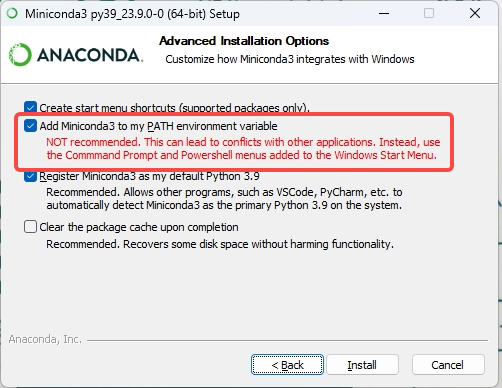
\includegraphics[width=.6\linewidth]{part/软件工程/环境搭建/虚拟环境/anaconda/pic/miniconda_windows环境变量.png}
      \caption{\label{fig:miniconda_windows环境变量}windows 安装miniconda配置环境变量}
\end{figure}

\reminder{\lefthand}{就算这步没有选择，可以安装以后手动配置环境变量，但是这样做会更麻烦一些。}

如图\ref{fig:miniconda_windows环境变量}所示，勾选上配置环境变量，然后点击下一步，然后点击安装，等待安装完成。

如果安装成功，可以在命令行中输入\codeinline{conda}，如果出现如图\ref{fig:conda安装成功}所示的结果，说明安装成功。
\begin{figure}[htbp]
    \centering 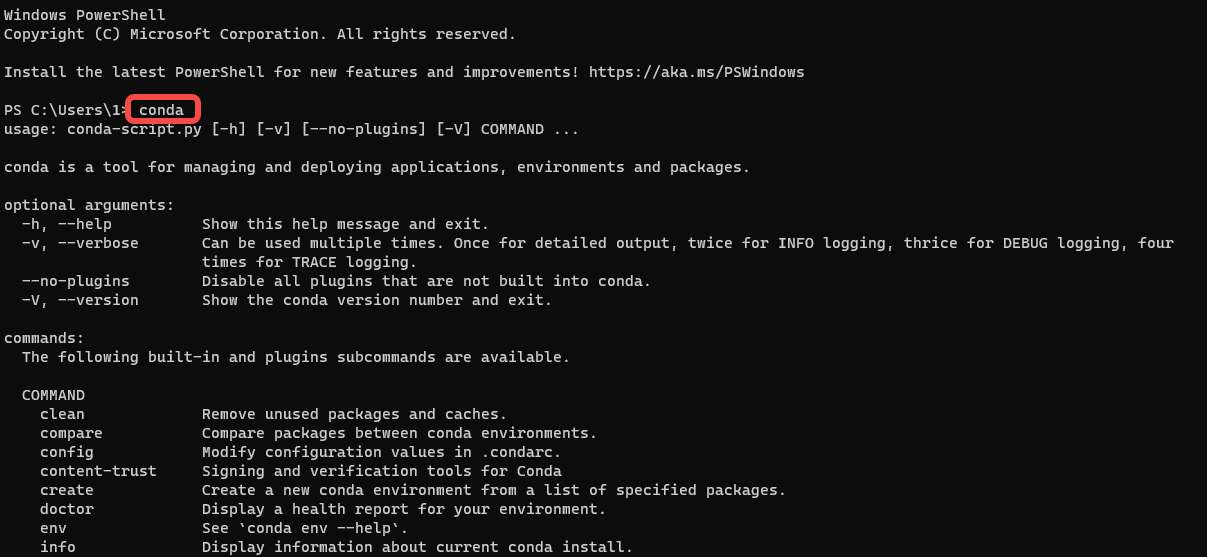
\includegraphics[width=.6\linewidth]{part/软件工程/环境搭建/虚拟环境/anaconda/pic/conda安装成功.png}
      \caption{\label{fig:conda安装成功}conda安装成功检验}
\end{figure}


\section{配置国内源}
\label{sec:use_conda_config}
各系统都可以通过修改用户目录下的 \codeinline{.condarc} 文件来使用 TUNA 镜像源
\subsection{linux}
\label{sec:use_conda_config_linux}
\begin{lstlisting}[style=demostyle,numbers=none]
$> vim ~/.condarc
channels:
  - defaults
show_channel_urls: true
default_channels:
  - https://mirrors.tuna.tsinghua.edu.cn/anaconda/pkgs/main
  - https://mirrors.tuna.tsinghua.edu.cn/anaconda/pkgs/r
  - https://mirrors.tuna.tsinghua.edu.cn/anaconda/pkgs/msys2
custom_channels:
  conda-forge: https://mirrors.tuna.tsinghua.edu.cn/anaconda/cloud
  msys2: https://mirrors.tuna.tsinghua.edu.cn/anaconda/cloud
  bioconda: https://mirrors.tuna.tsinghua.edu.cn/anaconda/cloud
  menpo: https://mirrors.tuna.tsinghua.edu.cn/anaconda/cloud
  pytorch: https://mirrors.tuna.tsinghua.edu.cn/anaconda/cloud
  pytorch-lts: https://mirrors.tuna.tsinghua.edu.cn/anaconda/cloud
  simpleitk: https://mirrors.tuna.tsinghua.edu.cn/anaconda/cloud
  deepmodeling: https://mirrors.tuna.tsinghua.edu.cn/anaconda/cloud/
 
$> conda info
\end{lstlisting}
\begin{figure}[htbp]
    \centering 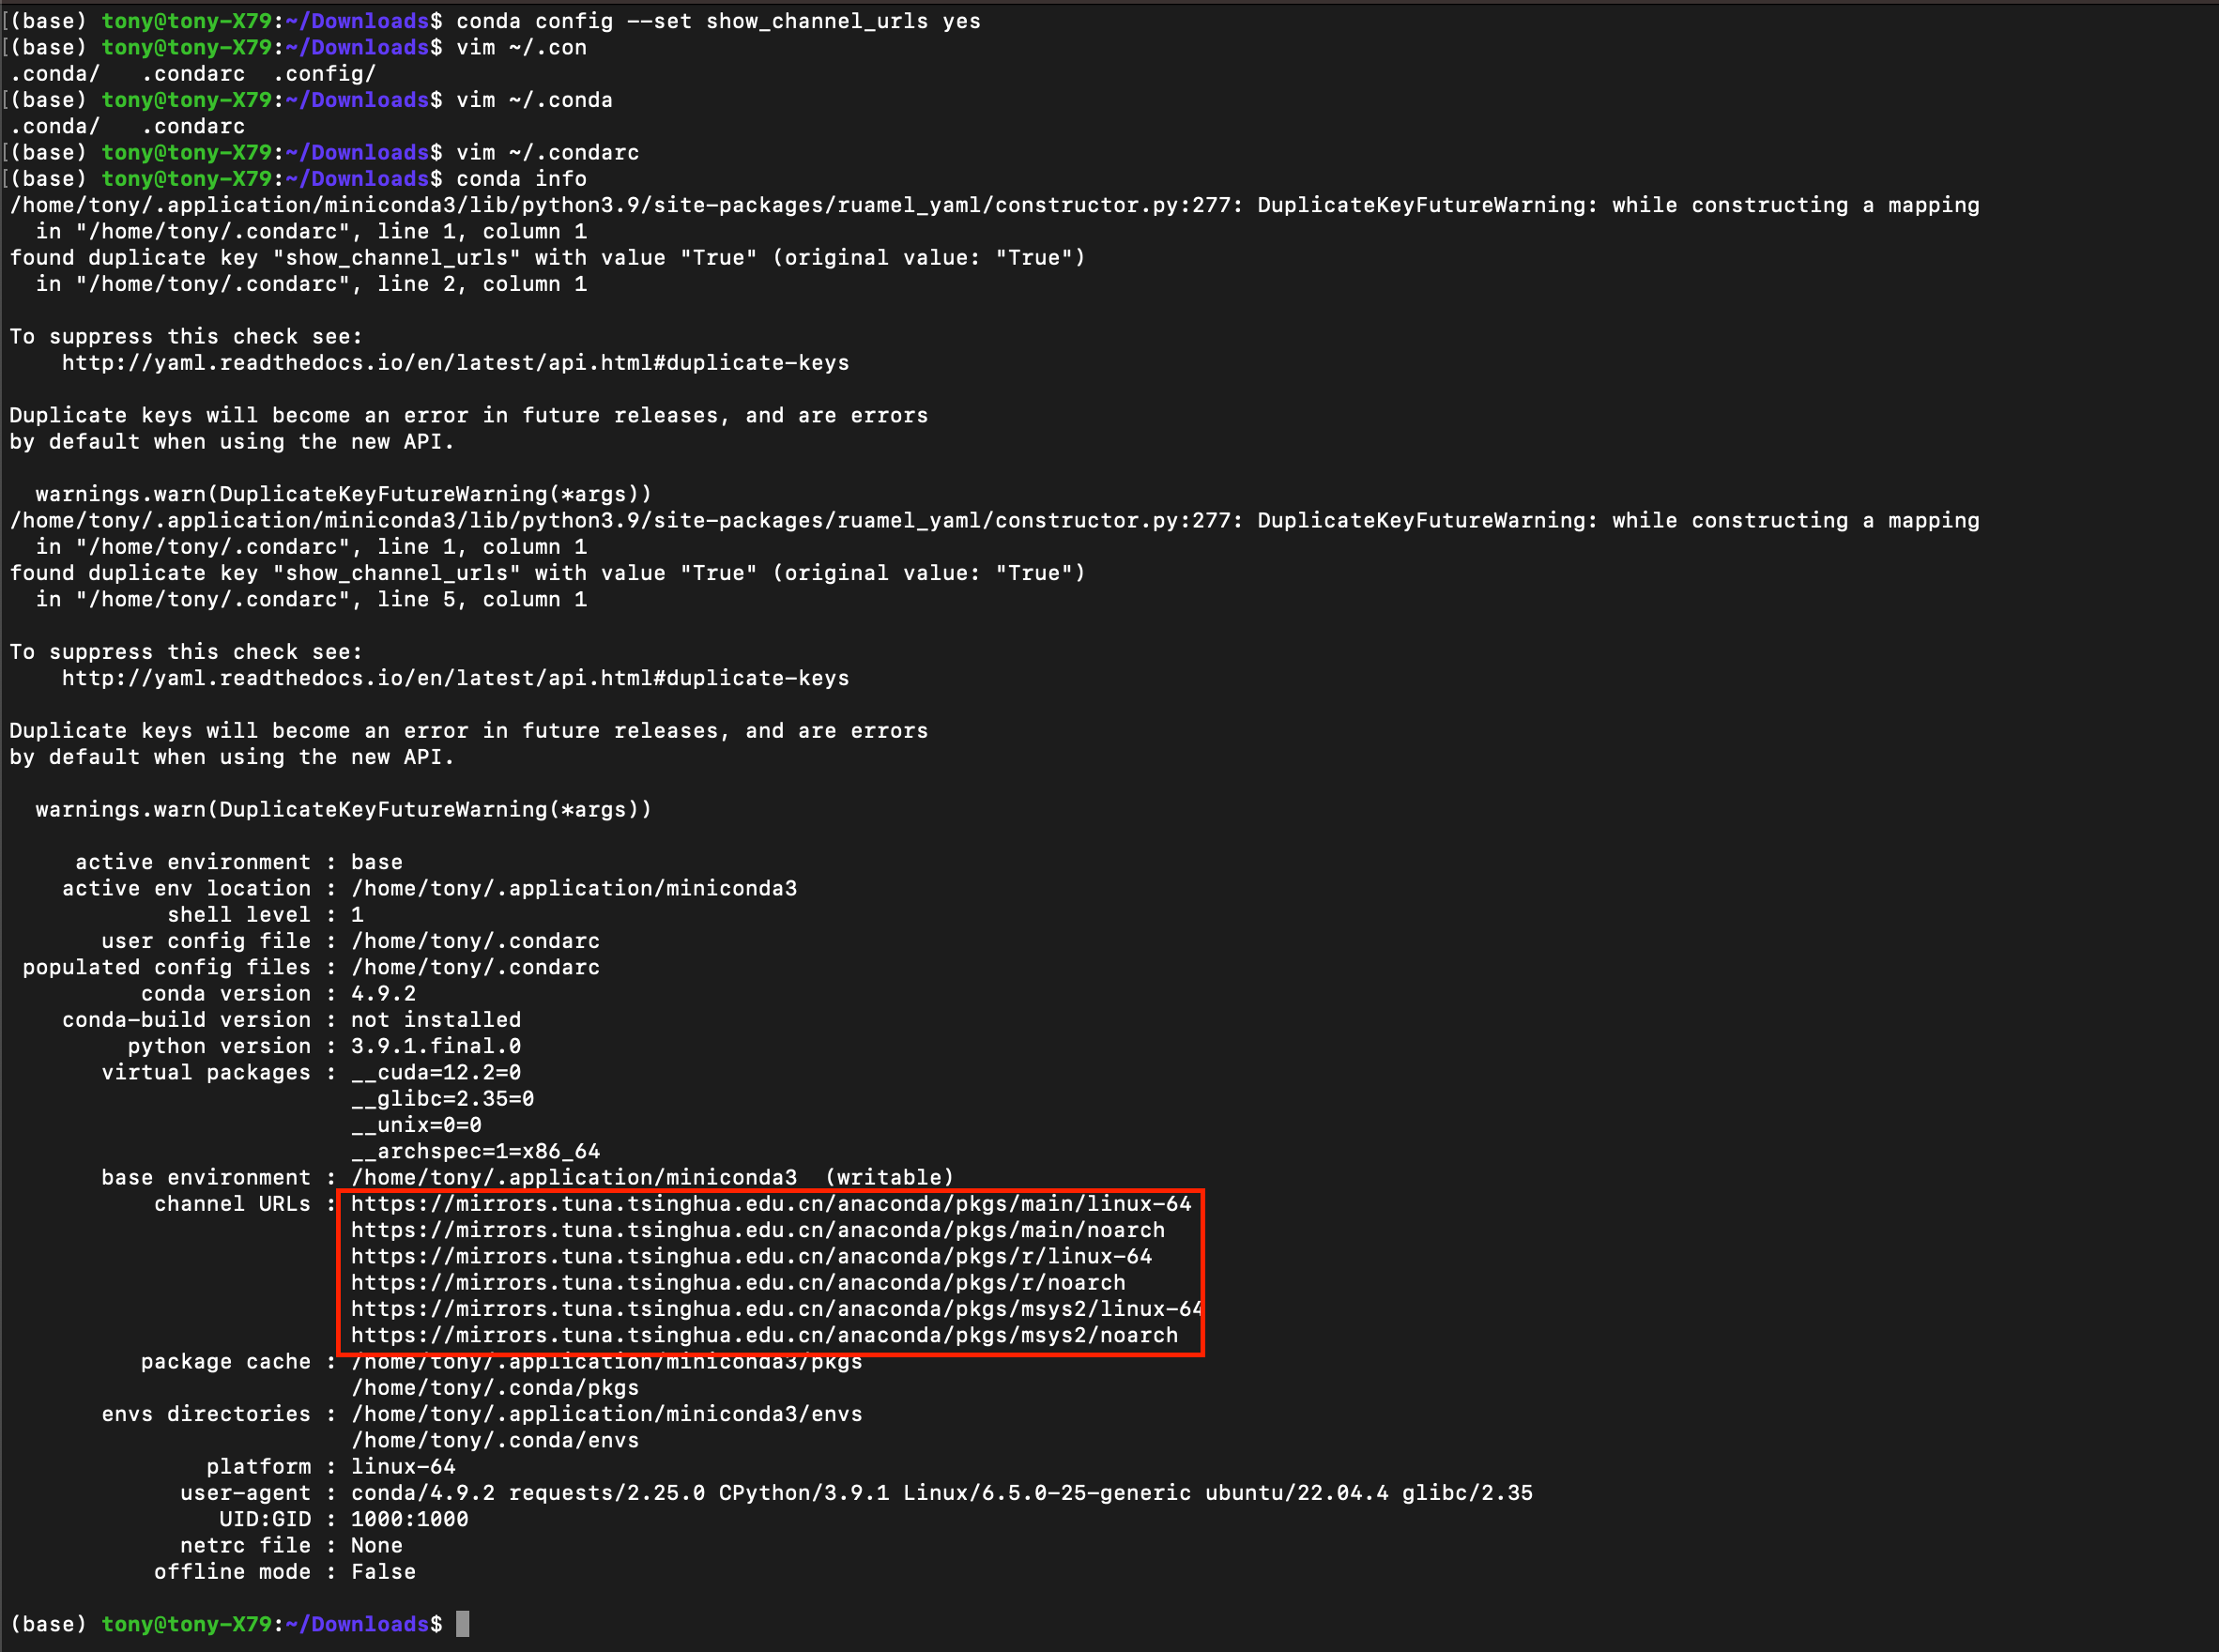
\includegraphics[width=.6\linewidth]{part/软件工程/环境搭建/虚拟环境/anaconda/pic/linux_conda使用终端配置国内源.png}
      \caption{\label{fig:linux_conda使用终端配置国内源}conda使用终端配置国内源}
\end{figure}

\subsection{windows}
\subsubsection{手动配置}
Windows 用户无法直接创建名为 \codeinline{.condarc} 的文件，可先执行 

\begin{lstlisting}[style=demostyle,numbers=none]
conda config --set show_channel_urls yes 
\end{lstlisting}
生成该文件之后再修改。
\begin{lstlisting}[style=demostyle,numbers=none]
show_channel_urls: true
channels:
  - defaults
default_channels:
  - https://mirrors.tuna.tsinghua.edu.cn/anaconda/pkgs/main
  - https://mirrors.tuna.tsinghua.edu.cn/anaconda/pkgs/r
  - https://mirrors.tuna.tsinghua.edu.cn/anaconda/pkgs/msys2
custom_channels:
  conda-forge: https://mirrors.tuna.tsinghua.edu.cn/anaconda/cloud
  msys2: https://mirrors.tuna.tsinghua.edu.cn/anaconda/cloud
  bioconda: https://mirrors.tuna.tsinghua.edu.cn/anaconda/cloud
  menpo: https://mirrors.tuna.tsinghua.edu.cn/anaconda/cloud
  pytorch: https://mirrors.tuna.tsinghua.edu.cn/anaconda/cloud
  pytorch-lts: https://mirrors.tuna.tsinghua.edu.cn/anaconda/cloud
  simpleitk: https://mirrors.tuna.tsinghua.edu.cn/anaconda/cloud
  deepmodeling: https://mirrors.tuna.tsinghua.edu.cn/anaconda/cloud/
\end{lstlisting}
\begin{figure}[htbp]
    \centering 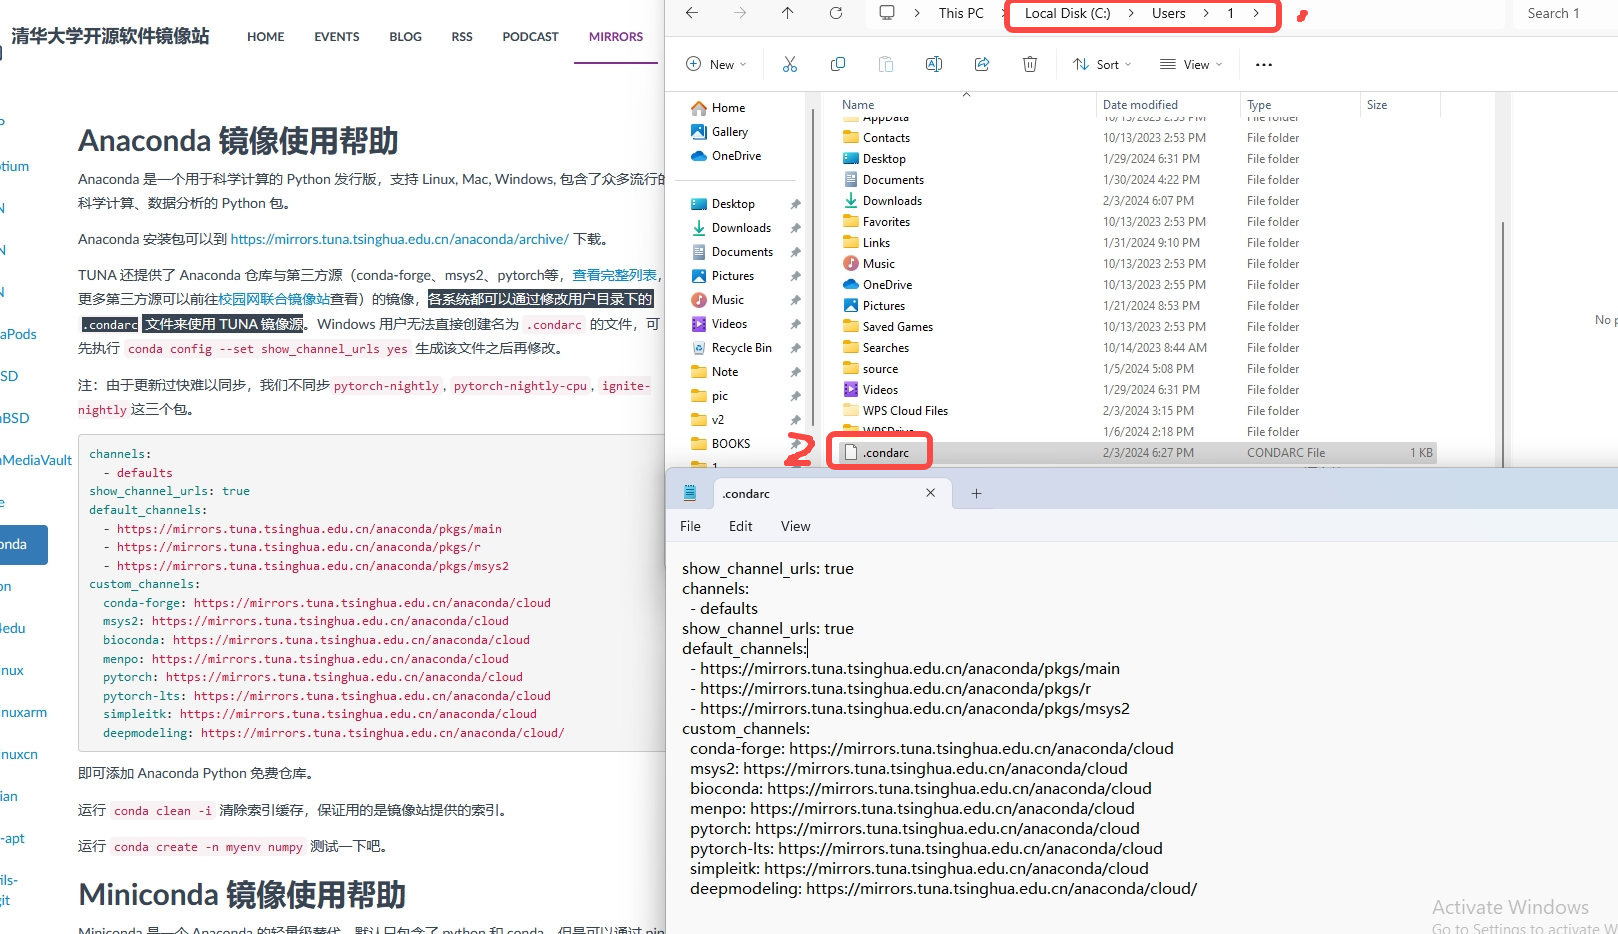
\includegraphics[width=.6\linewidth]{part/软件工程/环境搭建/虚拟环境/anaconda/pic/windows_conda使用配置文件配置国内源.png}
      \caption{\label{fig:windows_conda使用配置文件配置国内源}conda使用配置文件配置国内源}
\end{figure}

\subsubsection{命令行配置}
\label{sec:use_conda_config_windows_cmd}
如果嫌麻烦，可以直接在命令行中输入
\begin{lstlisting}[style=demostyle,numbers=none]
# 配置中科大源    
conda config --add channels https://mirrors.ustc.edu.cn/anaconda/pkgs/main/
conda config --add channels https://mirrors.ustc.edu.cn/anaconda/pkgs/free/
conda config --add channels https://mirrors.ustc.edu.cn/anaconda/cloud/conda-forge/
conda config --add channels https://mirrors.ustc.edu.cn/anaconda/cloud/msys2/
conda config --add channels https://mirrors.ustc.edu.cn/anaconda/cloud/bioconda/
conda config --add channels https://mirrors.ustc.edu.cn/anaconda/cloud/menpo/
conda config --add channels https://mirrors.ustc.edu.cn/anaconda/cloud/
# 阿里镜像源
conda config --add channels https://mirrors.aliyun.com/pypi/simple/
# 清华镜像源
conda config --add channels https://mirrors.tuna.tsinghua.edu.cn/anaconda/pkgs/main
conda config --add channels https://mirrors.tuna.tsinghua.edu.cn/anaconda/pkgs/r
conda config --add channels https://mirrors.tuna.tsinghua.edu.cn/anaconda/pkgs/msys2
# 清除索引缓存，保证用的是镜像站提供的索引
conda clean -i
# 显示检索路径，每次安装包时会将包源路径显示出来
conda config --set show_channel_urls yes
conda config --set always_yes True
# 显示所有镜像通道路径命令
conda config --show channels
# conda在指定环境下安装包
conda install -n machine_algorithm matplotlib
\end{lstlisting}    
\begin{figure}[htbp]
    \centering 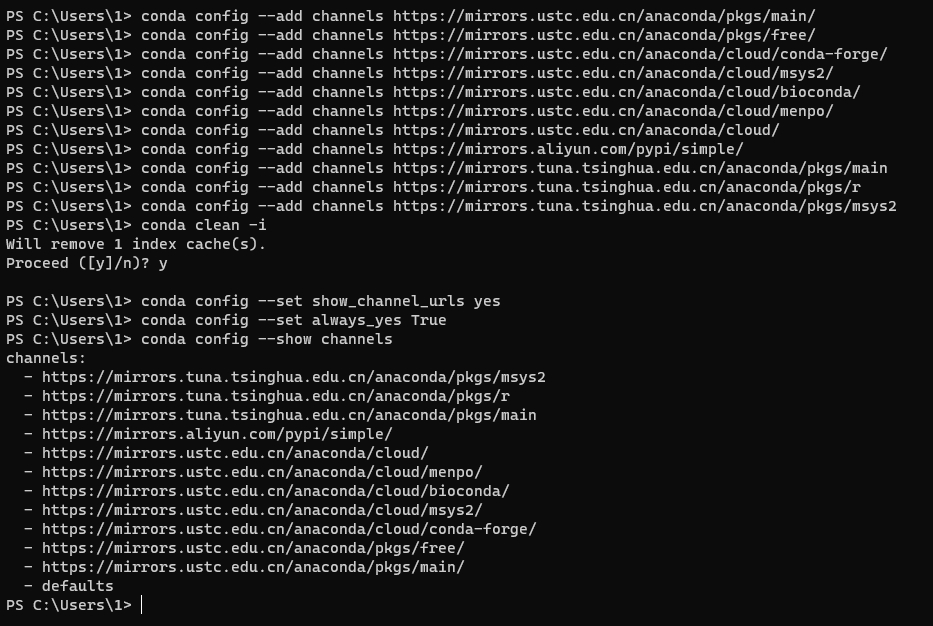
\includegraphics[width=.6\linewidth]{part/软件工程/环境搭建/虚拟环境/anaconda/pic/windows_conda使用终端配置国内源.png}
      \caption{\label{fig:windows_conda使用终端配置国内源}conda使用终端配置国内源}
\end{figure}

\subsubsection{移除镜像}
\label{sec:use_conda_config_windows_remove}
如果想要移除镜像，可以在命令行中输入
\begin{lstlisting}[style=demostyle,numbers=none]
conda config --remove channels 源名称或链接 
\end{lstlisting}    

\subsubsection{验证}
\label{sec:use_conda_config_windows_verify}
验证是否配置成功，可以在命令行中输入
\begin{lstlisting}[style=demostyle,numbers=none]
conda config --show-sources
# 或
conda info
\end{lstlisting}
如果出现如图\ref{fig:windows_conda使用终端配置国内源}所示的结果，说明配置成功。

\section{虚拟环境}
像Conda这样的包管理工具，管理的是\textcolor{YBXPurple}{虚拟环境}
\subsection{修改默认虚拟环境路径}
\begin{figure}[htbp]
    \centering 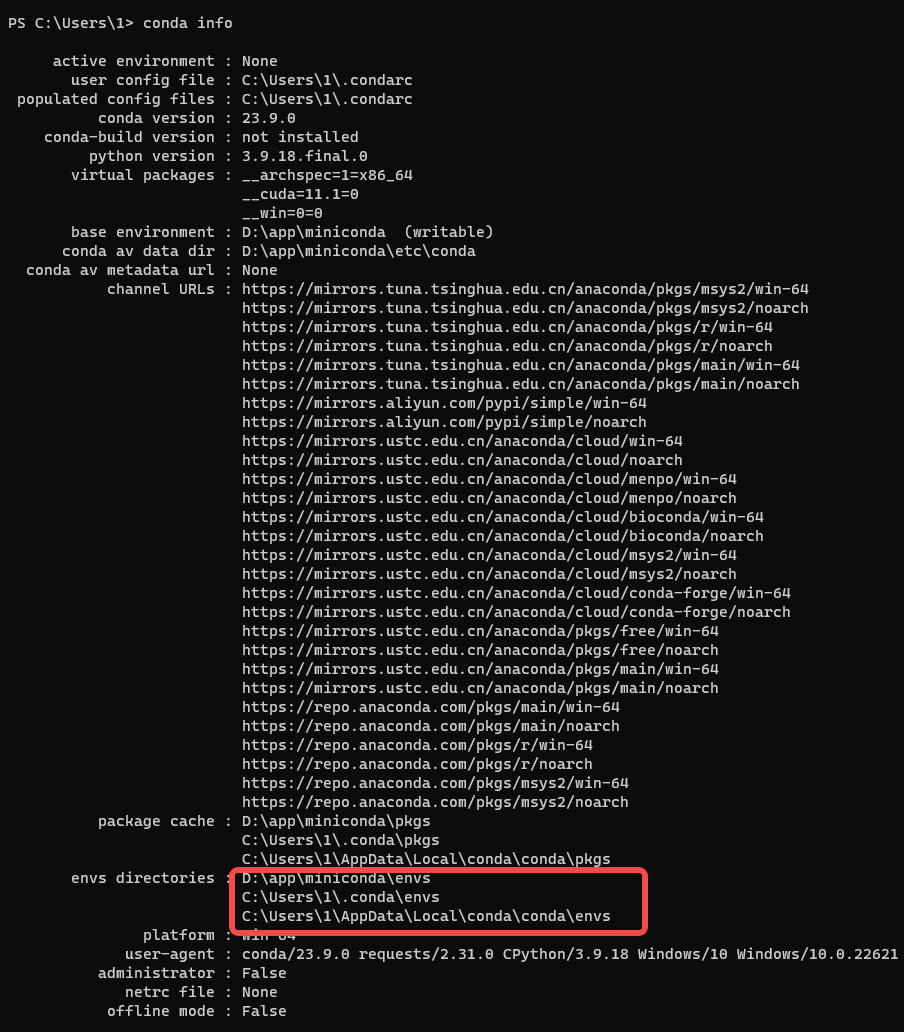
\includegraphics[width=.6\linewidth]{part/软件工程/环境搭建/虚拟环境/anaconda/pic/默认虚拟环境的默认路径.png}
      \caption{\label{fig:默认虚拟环境的默认路径}默认虚拟环境的默认路径}
\end{figure}

\subsubsection{Linux}
\begin{lstlisting}[style=demostyle,numbers=none]
$> mkdir  -p /home/tony/.local/conda_env # Linux
$> cat ~/.condarc
channels:
  - defaults
show_channel_urls: true
default_channels:
  - https://mirrors.tuna.tsinghua.edu.cn/anaconda/pkgs/main
  - https://mirrors.tuna.tsinghua.edu.cn/anaconda/pkgs/r
  - https://mirrors.tuna.tsinghua.edu.cn/anaconda/pkgs/msys2
custom_channels:
  conda-forge: https://mirrors.tuna.tsinghua.edu.cn/anaconda/cloud
  msys2: https://mirrors.tuna.tsinghua.edu.cn/anaconda/cloud
  bioconda: https://mirrors.tuna.tsinghua.edu.cn/anaconda/cloud
  menpo: https://mirrors.tuna.tsinghua.edu.cn/anaconda/cloud
  pytorch: https://mirrors.tuna.tsinghua.edu.cn/anaconda/cloud
  pytorch-lts: https://mirrors.tuna.tsinghua.edu.cn/anaconda/cloud
  simpleitk: https://mirrors.tuna.tsinghua.edu.cn/anaconda/cloud
  deepmodeling: https://mirrors.tuna.tsinghua.edu.cn/anaconda/cloud/

envs_dirs:
 - /home/tony/.local/conda_env
\end{lstlisting}  


\subsubsection{Windows}
在\codeinline{C:$\backslash$Users$\backslash$username$\backslash$.condarc}文件中添加如图\ref{fig:改变conda虚拟环境的默认路径}所示的内容，然后在命令行中输入

\begin{figure}[htbp]
    \centering 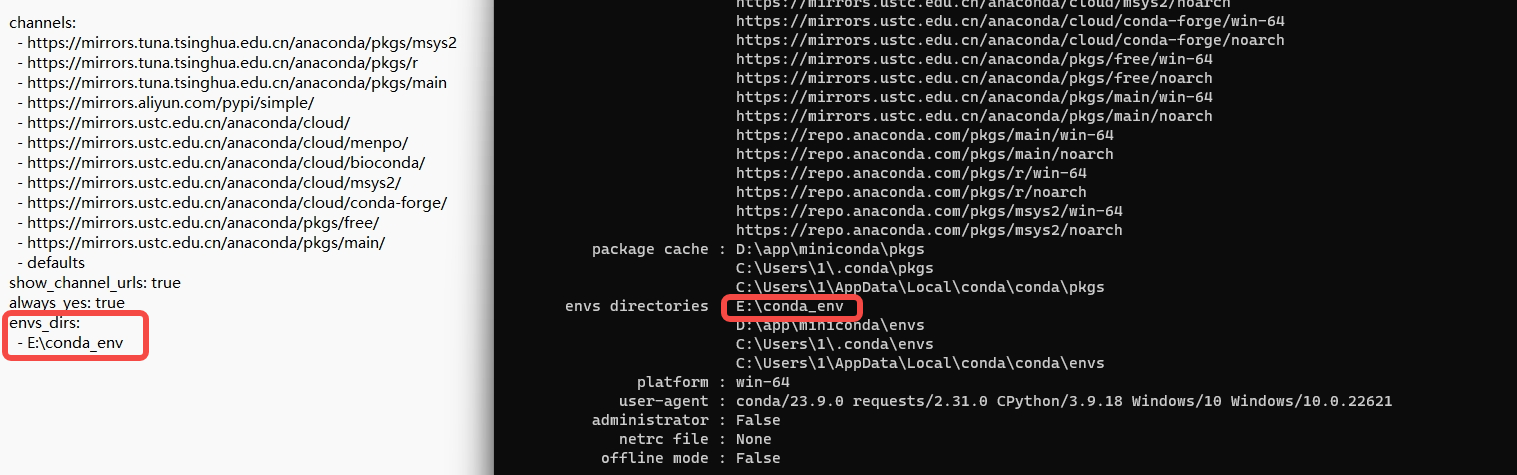
\includegraphics[width=.6\linewidth]{part/软件工程/环境搭建/虚拟环境/anaconda/pic/改变conda虚拟环境的默认路径.png}
      \caption{\label{fig:改变conda虚拟环境的默认路径}改变conda虚拟环境的默认路径}
\end{figure}


\subsection{创建虚拟环境}
\begin{lstlisting}[style=demostyle,numbers=none]
# 创建一个名为myenv的虚拟环境，指定Python版本是3.8，安装目录为E:\conda_env
conda create --name myenv python=3.9 -p E:\conda_env
\end{lstlisting}
\begin{figure}[htbp]
    \centering 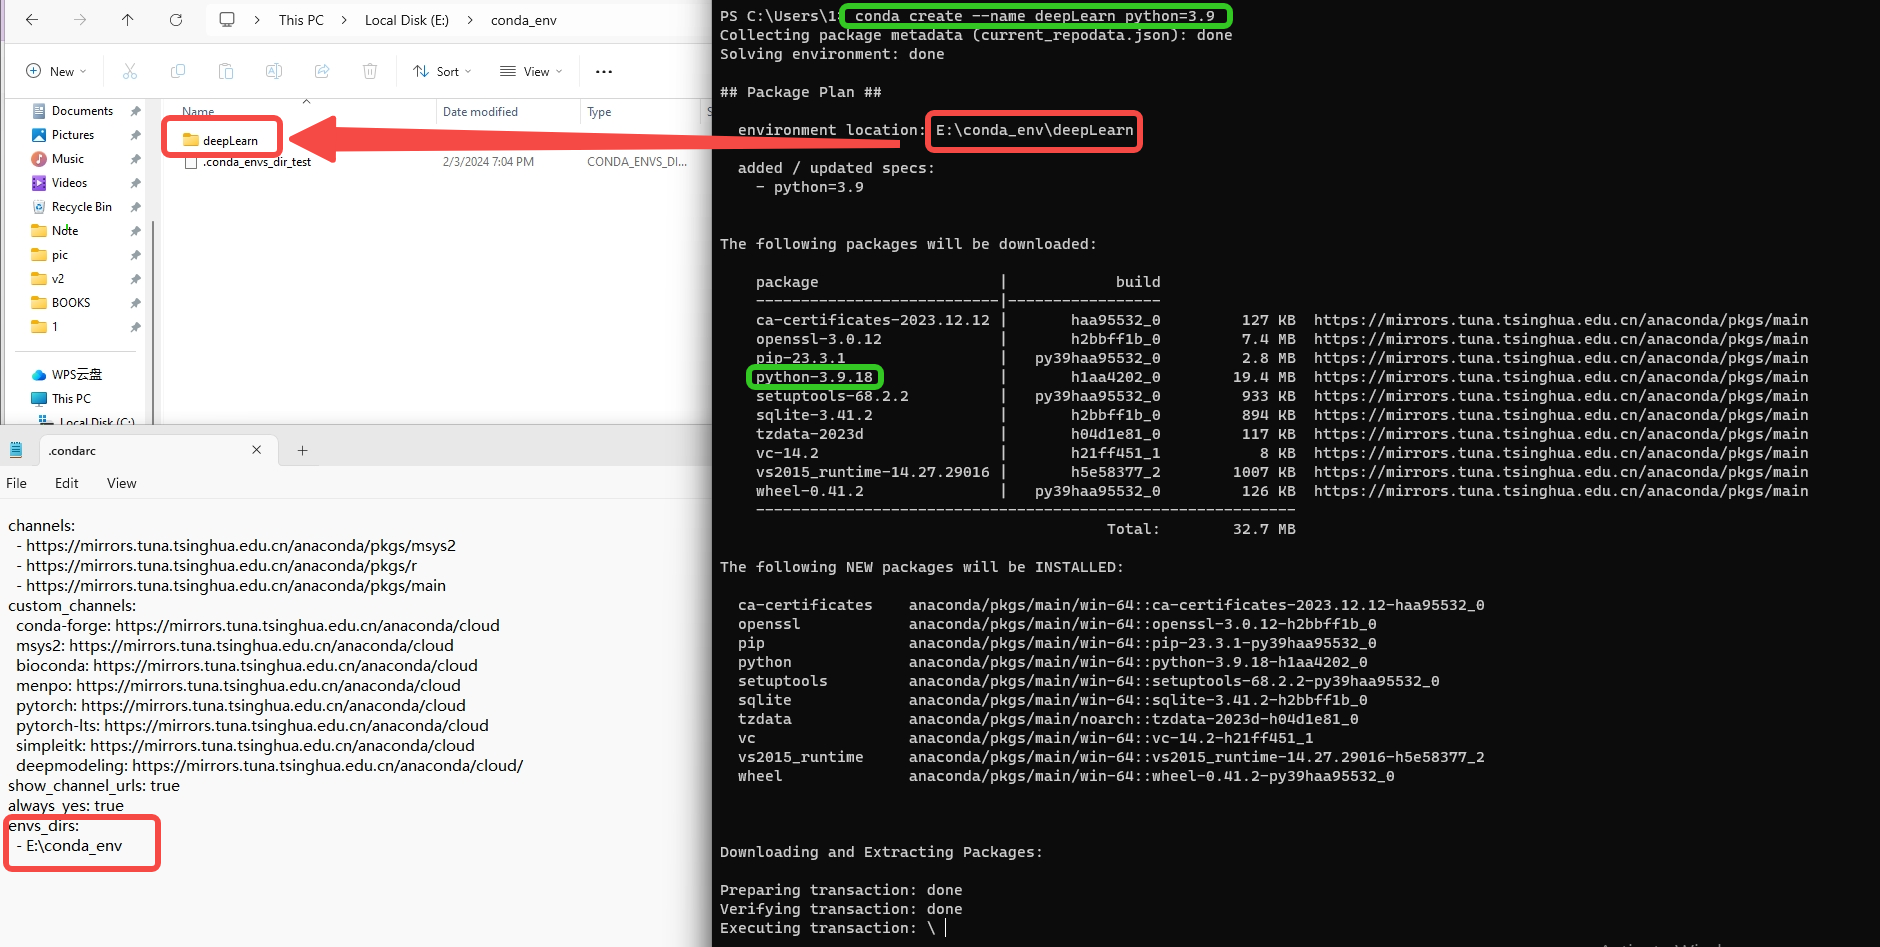
\includegraphics[width=.6\linewidth]{part/软件工程/环境搭建/虚拟环境/anaconda/pic/conda创建虚拟环境.png}
      \caption{\label{fig:conda创建虚拟环境}conda创建虚拟环境}
\end{figure}

\subsection{查看虚拟环境}
\label{subsubsec:use_conda_create_env_list}
\begin{lstlisting}[style=demostyle,numbers=none]
# 查看所有虚拟环境
conda info --envs
\end{lstlisting}
\begin{figure}[htbp]
    \centering 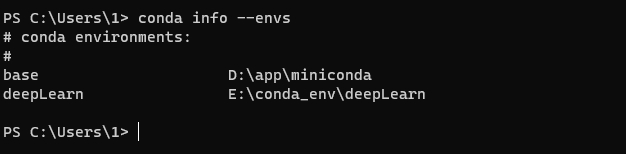
\includegraphics[width=.6\linewidth]{part/软件工程/环境搭建/虚拟环境/anaconda/pic/查看虚拟环境.png}
      \caption{\label{fig:查看虚拟环境}查看虚拟环境}
\end{figure}

\subsection{激活虚拟环境}
\begin{lstlisting}[style=demostyle,numbers=none]
# 激活虚拟环境
conda activate <env_name>
# 退出虚拟环境
conda deactivate
\end{lstlisting}

\subsection{删除虚拟环境}
在删除虚拟环境之前，需要先退出虚拟环境

\begin{lstlisting}[style=demostyle,numbers=none]
# 删除虚拟环境
conda remove --name <env_name> --all
\end{lstlisting}

\subsection{虚拟环境重新命名}
\begin{lstlisting}[style=demostyle,numbers=none]
# 重新命名虚拟环境
conda create --name new_name --clone old_name
\end{lstlisting}

\section{包管理}
\subsection{查询包}
\begin{lstlisting}[style=demostyle,numbers=none]
# 查询包
conda search <package_name>

# 安装指定版本的包
conda install <package_name>=<version>
\end{lstlisting}


\subsection{安装包}
\subsubsection{在线安装}
\subsubsubsection{conda安装}
conda安装包会自动安装相关依赖的包
\begin{lstlisting}[style=demostyle,numbers=none]
conda install pytorch torchvision torchaudio pytorch-cuda=11.8 -c pytorch -c nvidia
# -c 标志指定了要从哪个频道（channel）安装软件包。
# 频道是一组预先构建的二进制软件包的存储库，可以从中获取 Python 包和其他依赖项。频道可以位于 Anaconda 或第三方存储库中。
# 在使用 -c 标志时，可以在其后指定要使用的频道名称或 URL。
\end{lstlisting}
\begin{figure}[htbp]
    \centering 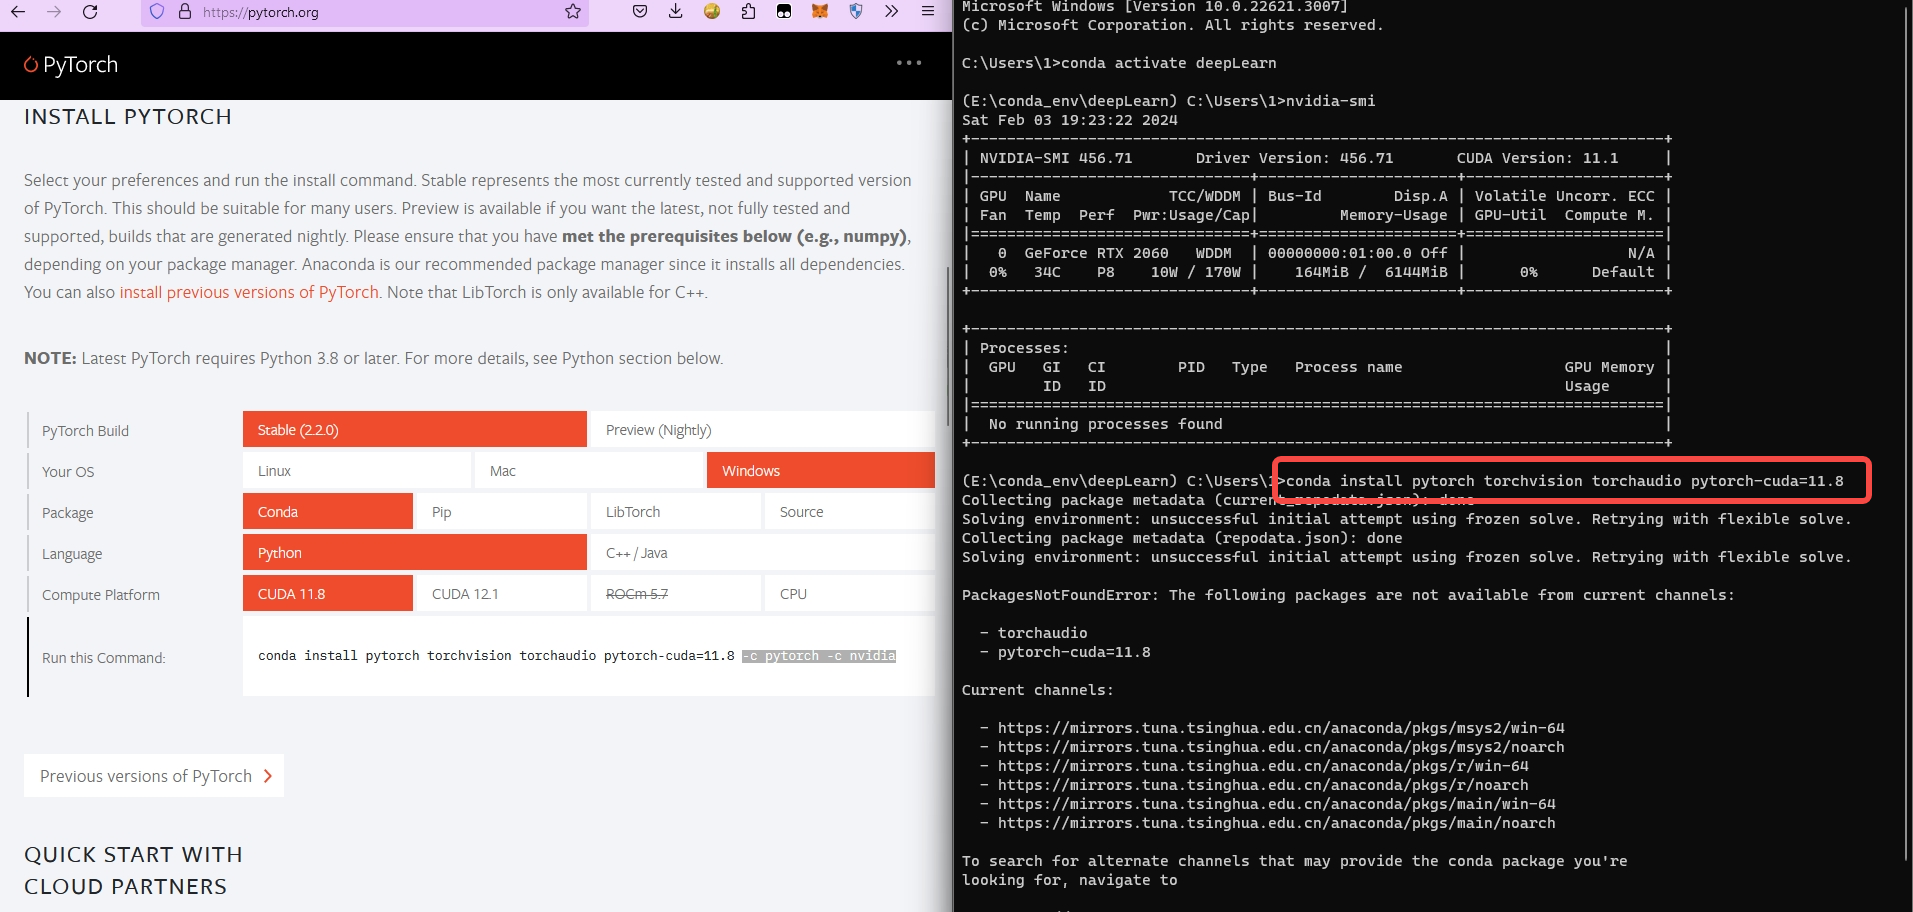
\includegraphics[width=.6\linewidth]{part/软件工程/环境搭建/虚拟环境/anaconda/pic/conda安装pytorch.png}
      \caption{\label{fig:conda安装pytorch}conda安装pytorch}
\end{figure}
\subsubsubsection{pip安装}
pip安装会比较快，但是相关依赖的包可能不会被安装
\begin{lstlisting}[style=demostyle,numbers=none]
pip3 install torch torchvision torchaudio --index-url https://download.pytorch.org/whl/cu118
\end{lstlisting}
\begin{figure}[htbp]
    \centering 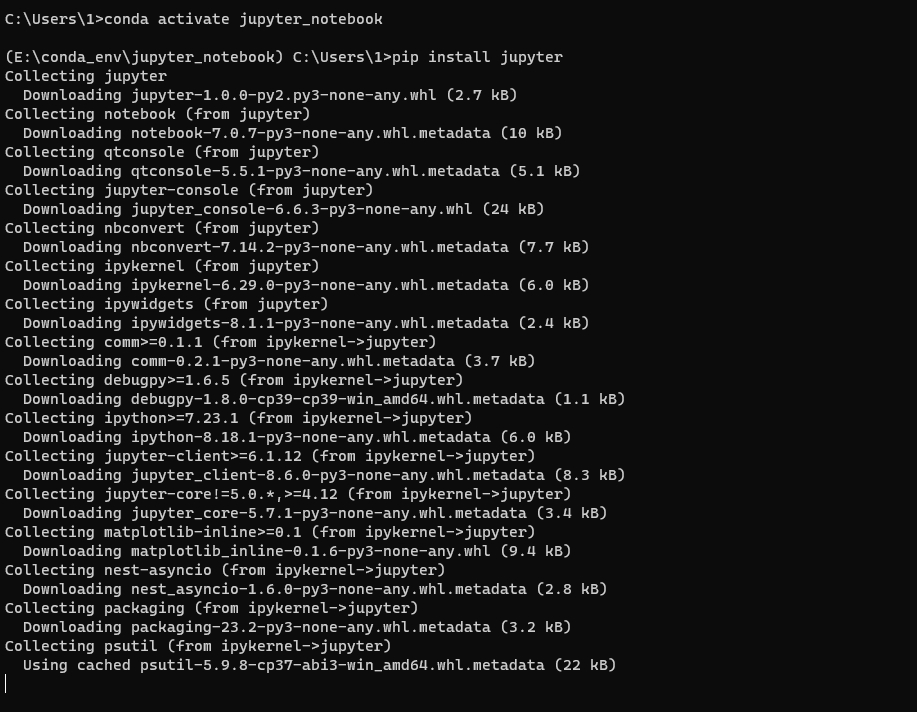
\includegraphics[width=.6\linewidth]{part/软件工程/环境搭建/虚拟环境/anaconda/pic/pip安装jupyter.png}
      \caption{\label{fig:pip安装jupyter}pip安装jupyter}
\end{figure}

\subsubsection{离线安装}
\label{subsubsec:install_package_offline}
如果有的包就一个可以到\href{https://pypi.org/}{pypi}上下载编译好的\codeinline{whl}文件，然后在命令行中输入
\begin{lstlisting}[style=demostyle,numbers=none]
pip install 包名
conda install 包名
\end{lstlisting}

\subsubsection{批量安装}
\label{subsubsec:install_package_batch}
事先写好一个\codeinline{requirements.txt}文件
\begin{lstlisting}[style=demostyle,numbers=none]
numpy
transformers==4.27.1
torch>=1.10
matplotlib
\end{lstlisting}    

然后在命令行中输入
\begin{lstlisting}[style=demostyle,numbers=none]
conda install --file requirements.txt
pip install -r requirements.txt
\end{lstlisting}

\subsection{卸载包}
\label{subsubsec:use_conda_package_remove}
\begin{lstlisting}[style=demostyle,numbers=none]
# 卸载包
conda remove <package_name>
conda uninstall <package_name>
\end{lstlisting}

\subsection{查看包}
\label{subsubsec:use_conda_package_list}
\begin{lstlisting}[style=demostyle,numbers=none]
# 查看所有已安装的包
conda list
# 查看指定环境下的包
conda list -n <env_name>
\end{lstlisting}

\subsection{更新包}
\label{subsubsec:use_conda_package_update}
\begin{lstlisting}[style=demostyle,numbers=none]
# 更新所有包
conda update --all

# 更新指定包
conda update <package_name>

## 更新conda本身
conda update conda
\end{lstlisting}

\subsection{清空缓存}
\label{subsubsec:use_conda_package_clean}
\begin{lstlisting}[style=demostyle,numbers=none]
# 清空缓存
conda clean --all
\end{lstlisting}

\section{Vscode配置}
\begin{figure}[htpb]
  \centering
  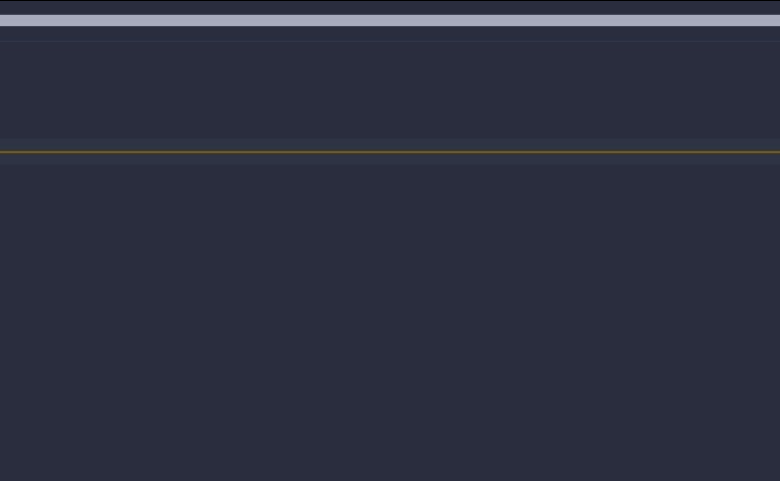
\includegraphics[width=0.6\textwidth]{part/软件工程/环境搭建/虚拟环境/anaconda/pic/vscode配置miniconda.png}
  \caption{修改python解释器}
  \label{fig:vscode配置miniconda-修改python解释器}
\end{figure}

\begin{figure}[htpb]
  \centering
  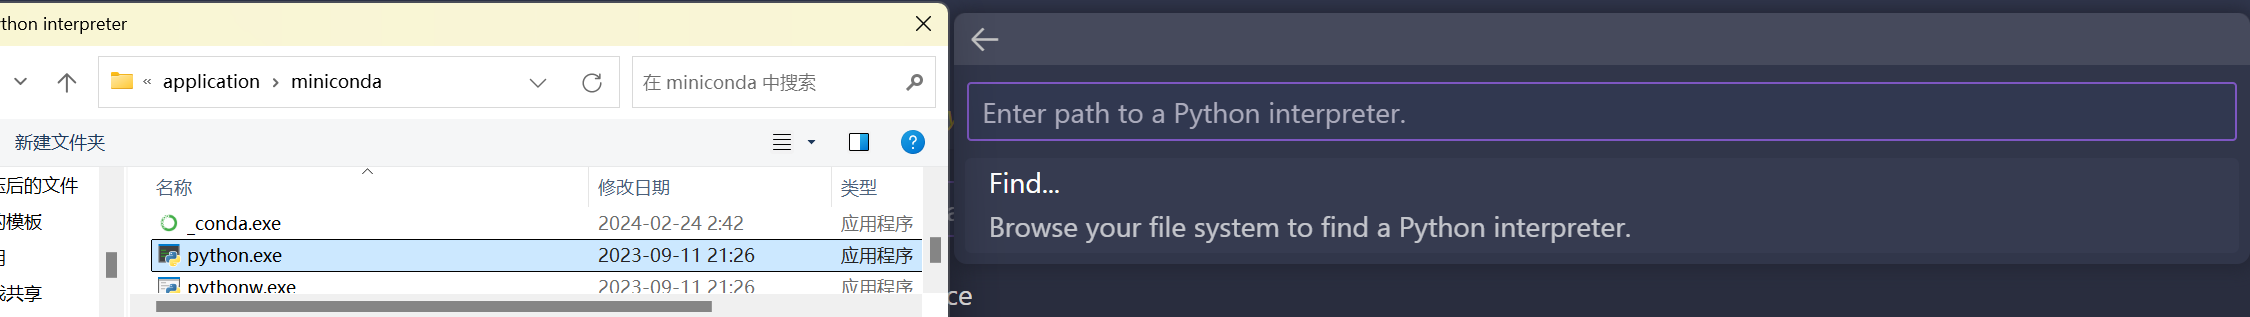
\includegraphics[width=0.6\textwidth]{part/软件工程/环境搭建/虚拟环境/anaconda/pic/选择conda的python解释器.png}
  \caption{选择conda的python解释器}
  \label{fig:选择conda的python解释器}
\end{figure}




\chapter{venv 环境}

\section{概述}
\codeinline{venv}就是用来为一个应用创建一套“隔离”的Python运行环境

\section{使用}
\begin{lstlisting}[style=demostyle,numbers=none]
# 创建虚拟环境
python -m venv my_env

# 激活虚拟环境
## Linux
source my_env/bin/activate
## Windows
my_env\Scripts\activate.bat

# 退出虚拟环境
deactivate
\end{lstlisting}

\section{常用命令}
\subsection{指定python版本}
\begin{lstlisting}[style=demostyle,numbers=none]
# 创建虚拟环境
python -m venv my_env --python=python3.6
\end{lstlisting}

\section{与Vscode结合}
\url{https://code.visualstudio.com/docs/python/environments}

%% Jupyter notebook
\chapter{Jupter Notebook}
\section{简介}
\label{sec:jupyter_intro}
\reminder{\lefthand}{Jupyter Notebook 建议仅用于学习目的，不推荐用于项目开发。}
Jupter Notebook是基于网页的用于交互计算的应用程序。

其实Jupter Notebook与Jupter lab没什么大的区别

其功能
\begin{enumerate}[label=\arabic*)]
    \item 开发
    \item 运行代码
    \item 文档编写
    \item 展示结果
\end{enumerate}

\subsection{notebook 运行逻辑}
Jupyter Notebook不仅仅是一个简单的web应用程序，它还需要关联指定的kernel，用于执行我们的代码。

\begin{figure}[htpb]
  \centering
  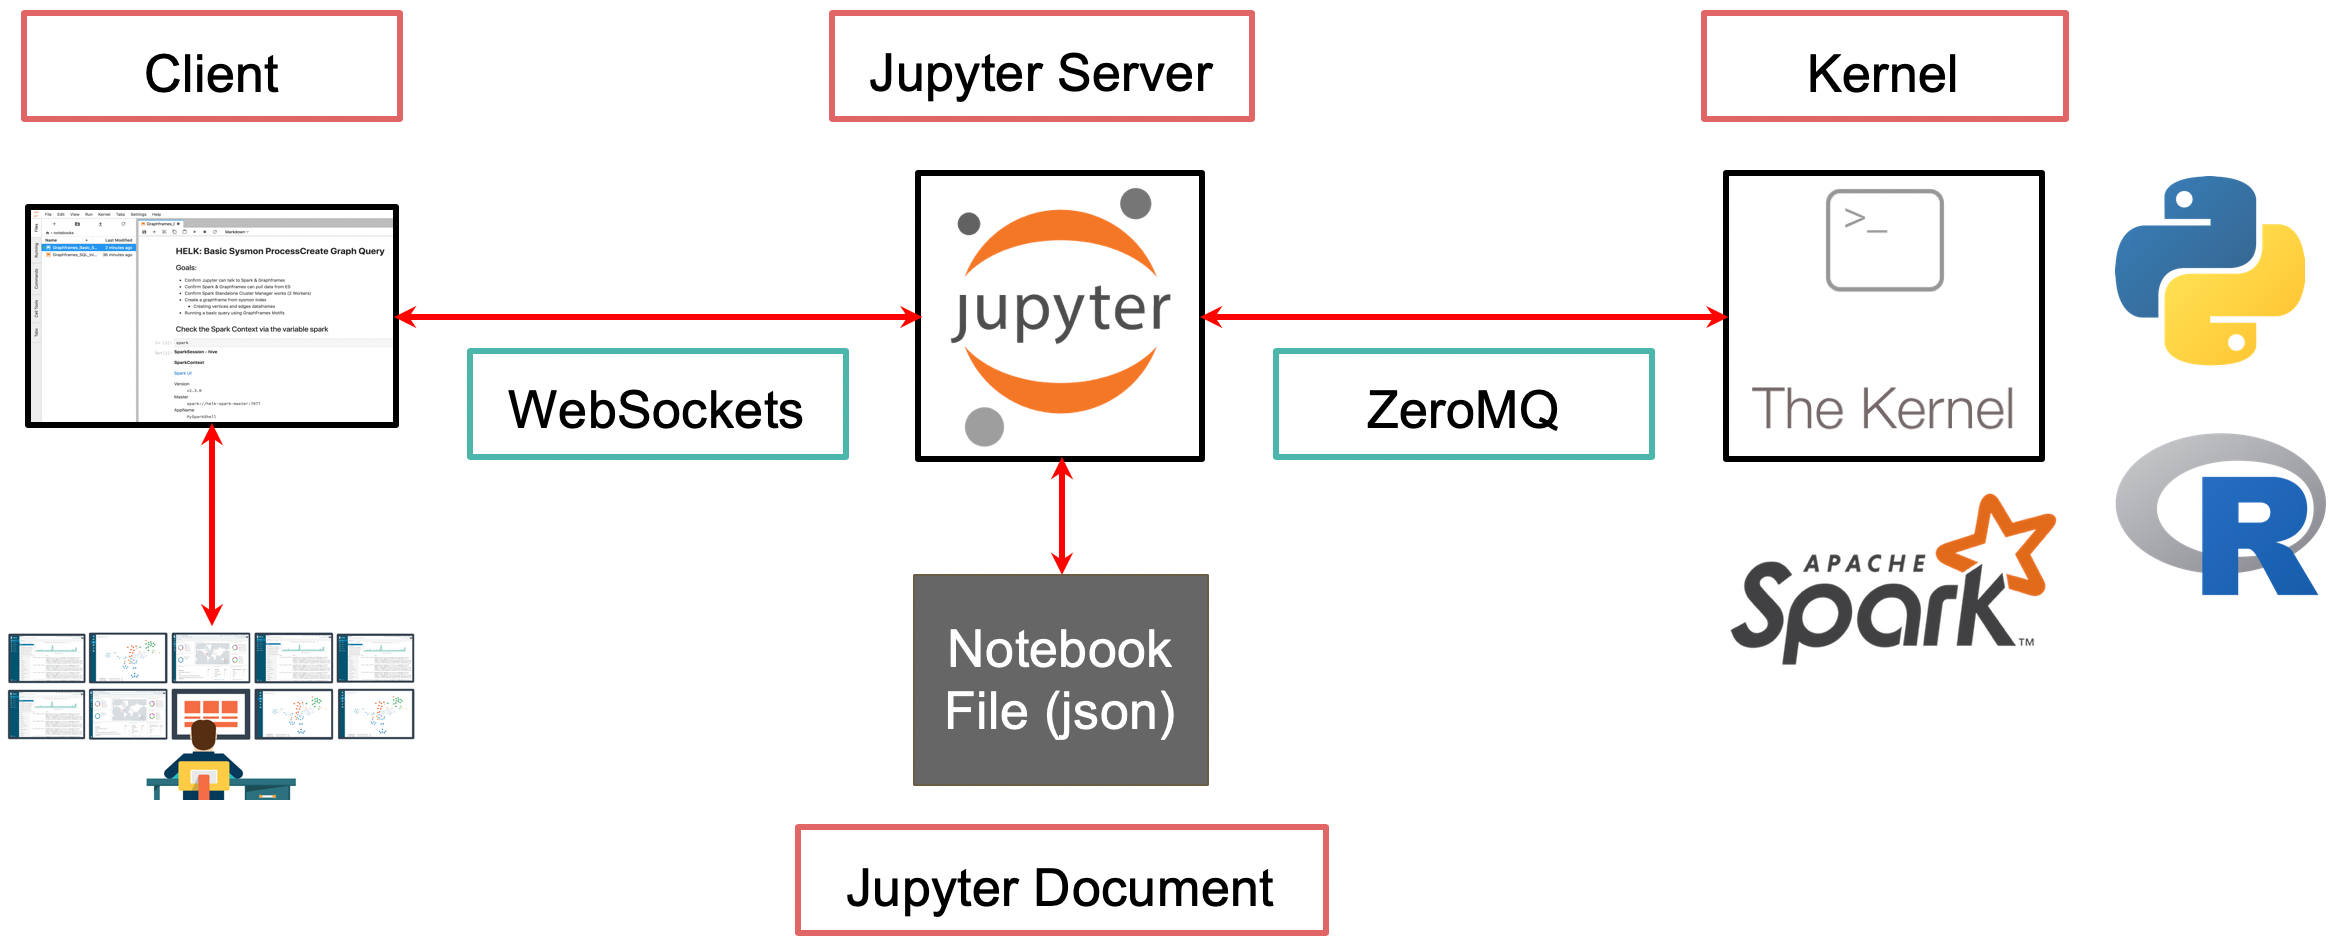
\includegraphics[width=0.6\textwidth]{part/软件工程/环境搭建/JupyterNotbook/pic/Jupyternotebook概述/jupyternotebook运行逻辑.png}
  \caption{Jupyter Notebook 运行逻辑}
  \label{fig:jupyternotebook运行逻辑}
\end{figure}

如图\ref{fig:jupyternotebook运行逻辑}所示，左边是用户写的代码，传输到中间的Jupyter server, server本身不能执行代码，server把代码传给Kernel，Kernel才是实际执行代码的组件，执行代码的地方。Kernel执行完代码，把结果返回给server，再返回到用户的网页。

Kernel不仅可以是python.exe，也可以是其他语言的解释器，如Julia, R等，更多kernel可以看支持的\href{https://github.com/jupyter/jupyter/wiki/Jupyter-kernels}{kernel列表}.

在pytorch开发中，kernel其实就是某一个python解释器——python.exe，我们需要为当前的notebook配置相应的kernel，来进入相应的虚拟环境，这样才能运行代码。

\section{安装}
\subsection{安装IPython(非必须)}
\begin{lstlisting}[style=demostyle,numbers=none]
# 安装
conda install ipython
# 或
pip install IPython # 安装IPython
\end{lstlisting}

\subsection{安装Jupyter}
\begin{lstlisting}[style=demostyle,numbers=none]
# 安装
conda install jupyter
# 或
pip install jupyter
\end{lstlisting}

\subsection{添加Kernel}
\begin{lstlisting}[style=demostyle,numbers=none]
# 1.进入虚拟环境
conda activate mypytorch
# 2.安装ipykernel工具包（安装jupyter）
conda install ipykernel
# 或
pip install ipykernel
# 3.为当前环境添加kernel
python -m ipykernel install --user --name=mypytorch
\end{lstlisting}

\subsection{代码补全}
\begin{lstlisting}[style=demostyle,numbers=none]
# 安装
pip install jupyter_contrib_nbextensions
## 有时会不匹配报错 pip install -i https://pypi.tuna.tsinghua.edu.cn/simple jupyter_contrib_nbextensions

conda install -c conda-forge jupyter_contrib_nbextensions
\end{lstlisting}

\section{使用}
\subsection{本地使用}
在那个目录下打开命令行，打开jupyter lab以后就是那个目录。
\begin{lstlisting}[style=demostyle,numbers=none]
# 切换到目标目录
cd 目标目录
# 激活虚拟环境
conda activate jupyter_notebook
# 在命令行中输入
jupyter notebook
# 或
jupyter lab # (推荐)更加强大的版本
\end{lstlisting}
\begin{figure}[htbp]
    \centering 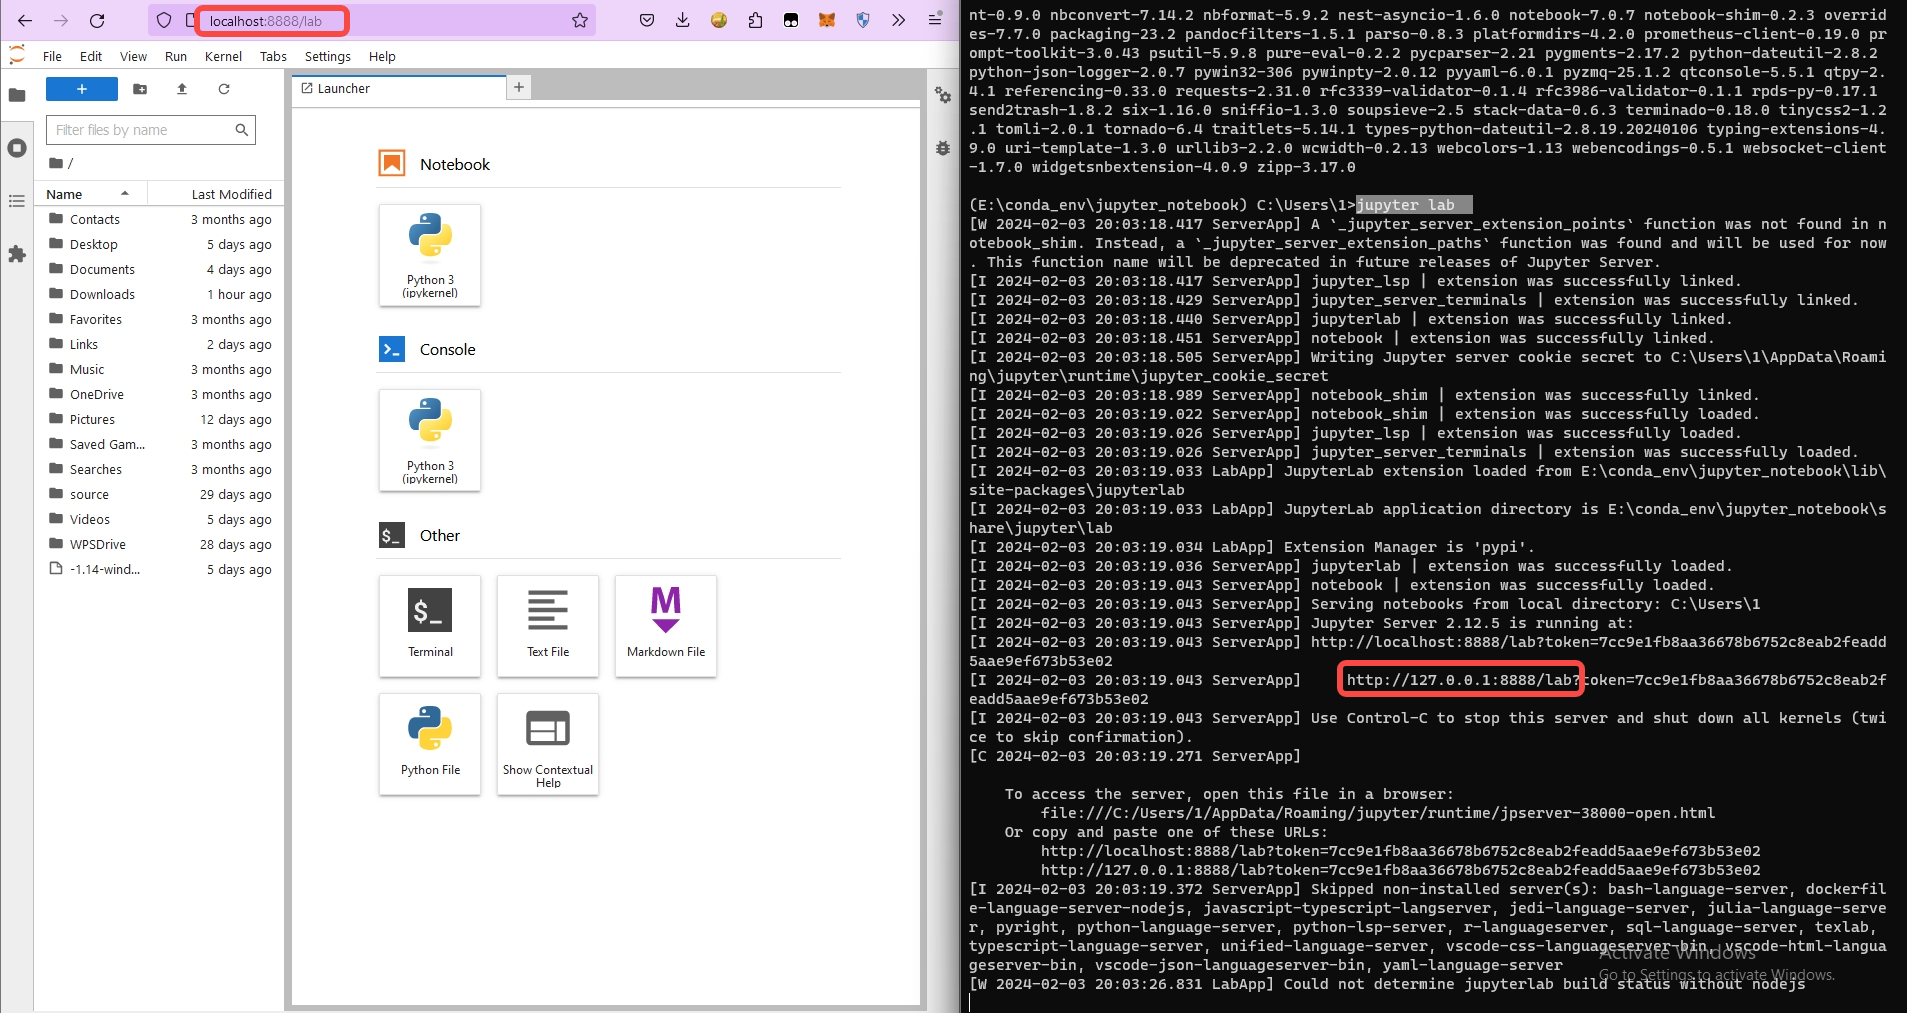
\includegraphics[width=.6\linewidth]{part/软件工程/环境搭建/JupyterNotbook/pic/Jupyternotebook概述/启动jupyter_lab.png}
      \caption{\label{fig:启动jupyter_lab}启动jupyter lab}
\end{figure}

\subsection{远程使用}
\subsubsection{远程服务器配置}
如图\ref{fig:配置远程连接JupterNotebook}所示，配置远程连接JupterNotebook。
\begin{lstlisting}[style=demostyle,numbers=none]
$(conda_env)> jupyter notebook --generate-config
Writing default config to: /home/tony/.jupyter/jupyter_notebook_config.py

(conda_env)> jupyter lab --generate-config
Writing default config to: /home/tony/.jupyter/jupyter_lab_config.py

$(conda_env)> vim ~/.jupyter/jupyter_notebook_config.py
c.NotebookApp.ip = '*'                     # 允许访问此服务器的 IP，星号表示任意 IP
c.NotebookApp.open_browser = False         # 运行时不打开本机浏览器
#c.NotebookApp.port = 8890                 # 使用端口，默认是 8888
c.NotebookApp.enable_mathjax = True        # 启用 MathJax
c.NotebookApp.allow_remote_access = True   #允许远程访问
#c.NotebookApp.allow_root = True           # 允许以root用户启动

$(conda_env)> jupyter notebook --no-browser --port=8888

$(conda_env)> jupyter lab --no-browser --port=8888
$(conda_env)> nohup jupyter lab --no-browser --port=8888 > $(date '+%Y-%m-%d-%H-%M-%S')-jupyter.log 2>&1 &
\end{lstlisting}

\begin{figure}[htbp]
    \centering 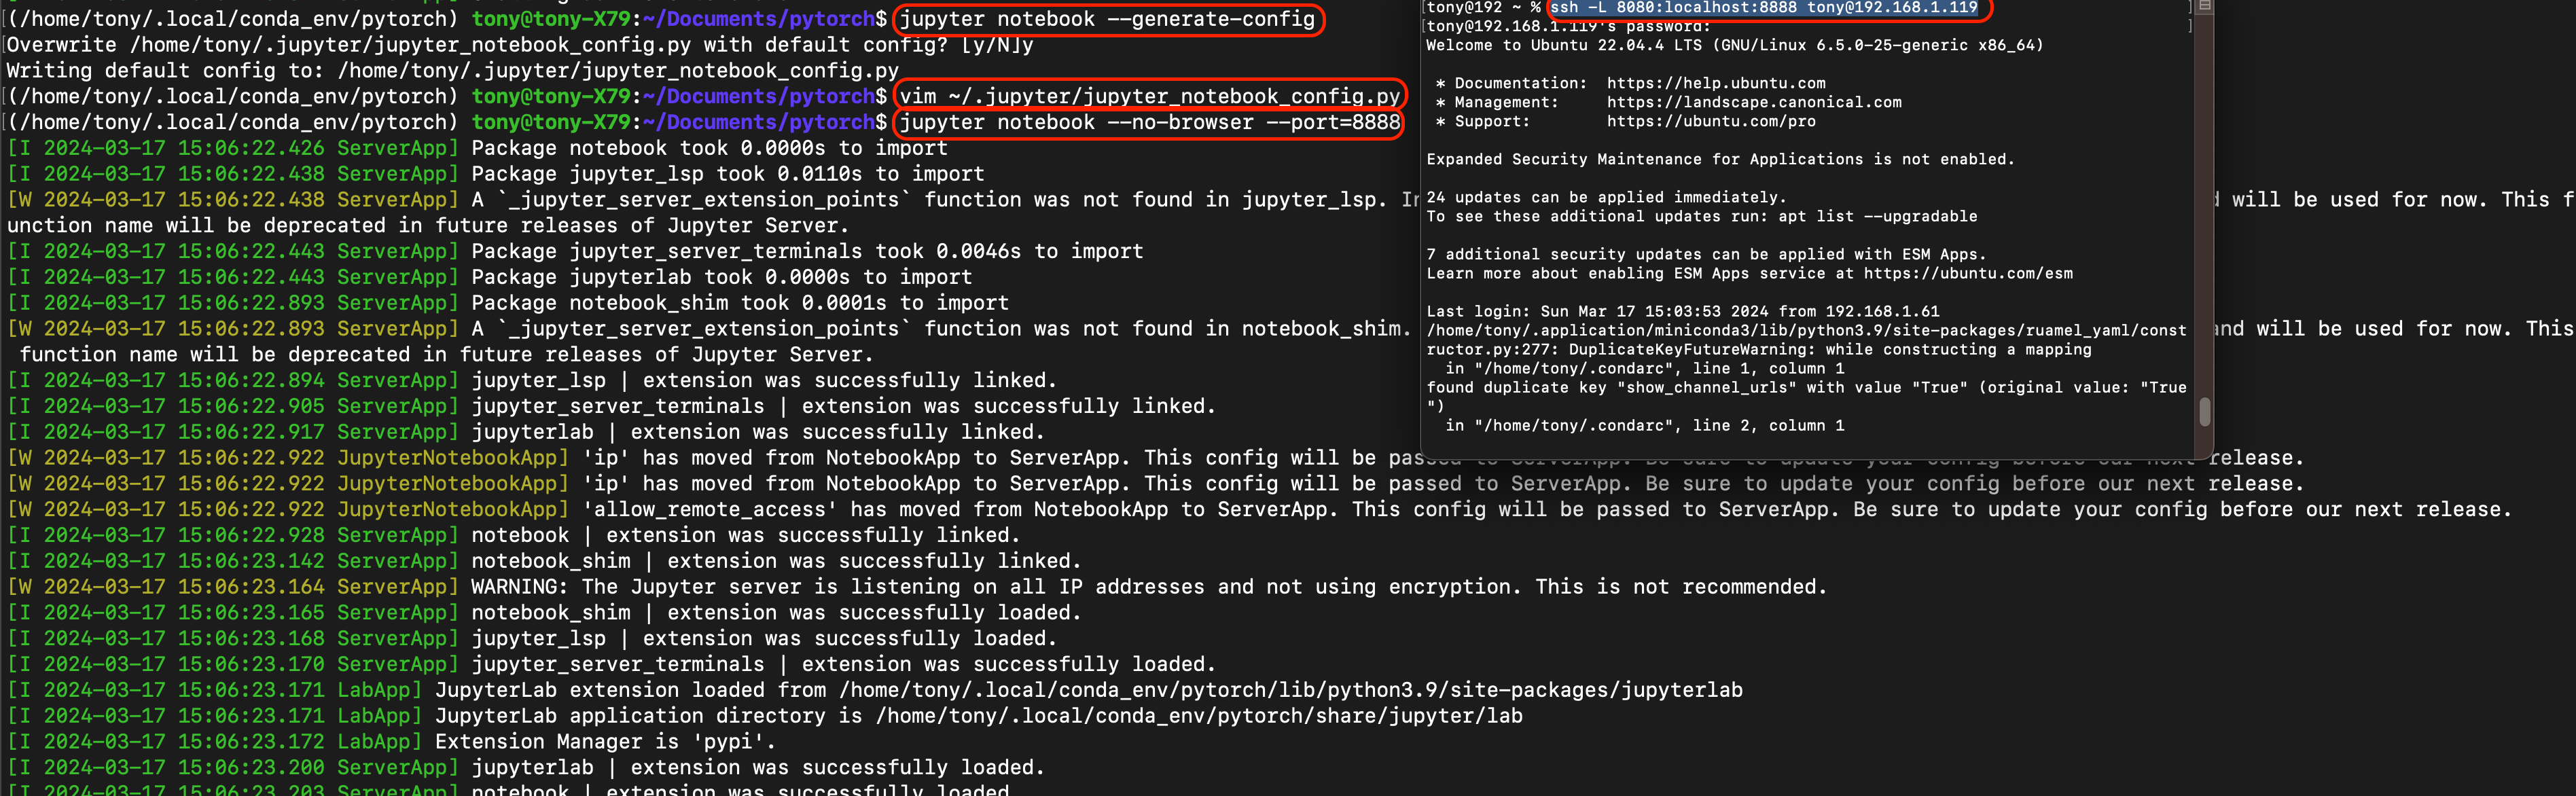
\includegraphics[width=.9\linewidth]{part/软件工程/环境搭建/JupyterNotbook/pic/Jupyternotebook概述/配置远程连接JupterNotebook.png}
      \caption{\label{fig:配置远程连接JupterNotebook}配置远程连接JupterNotebook}
\end{figure}

\subsubsection{本地访问远程JupterLab}
\subsubsubsection{配置防火墙访问}
\begin{lstlisting}[style=demostyle,numbers=none]
$(conda_env)> jupyter lab --no-browser --port=8888 # 在远程服务器上启动JupterLab
# 临时设置
$ sudo firewall-cmd --list-ports       # 列出所有开放都得端口
$ sudo firewall-cmd --add-port=8888/tcp # 添加临时的开放端口
$ sudo firewall-cmd --remove-port=8888/tcp # 关闭临时的开放端口

# 永久设置
$ firewall-cmd --list-ports --permanent # 查看所有永久开放的端口（默认为空）
$ sudo firewall-cmd --add-port=8888/tcp --permanent # 添加永久的开放端口
$ sudo firewall-cmd --remove-port=8888/tcp --permanent # 关闭永久的开放端口

# 配置结束后需要输入重载命令并重启防火墙以生效配置
$ sudo firewall-cmd --reload
$ sudo systemctl restart firewalld
\end{lstlisting}  

\begin{figure}[htbp]
  \centering 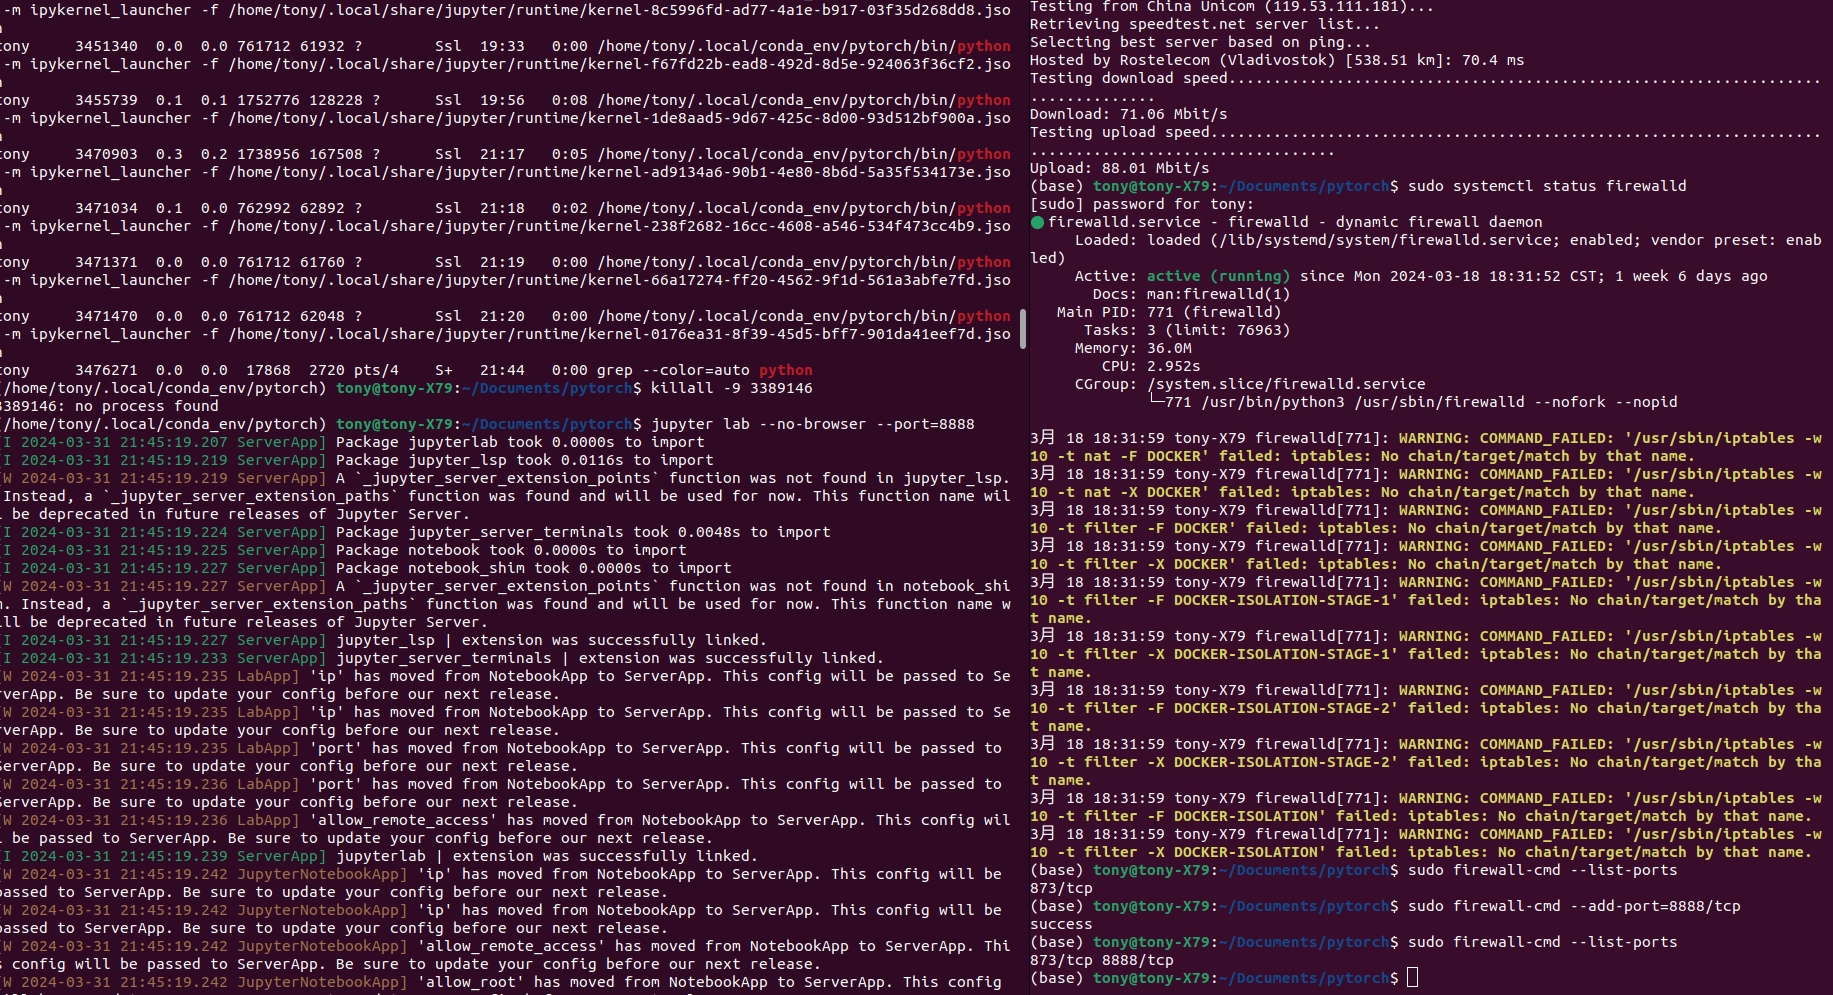
\includegraphics[width=.9\linewidth]{part/软件工程/环境搭建/JupyterNotbook/pic/Jupyternotebook概述/远程开启jupyter_lab防火墙.png}
    \caption{\label{fig:远程开启jupyterlab防火墙}远程开启jupyter lab防火墙}
\end{figure}

\begin{figure}[htbp]
  \centering 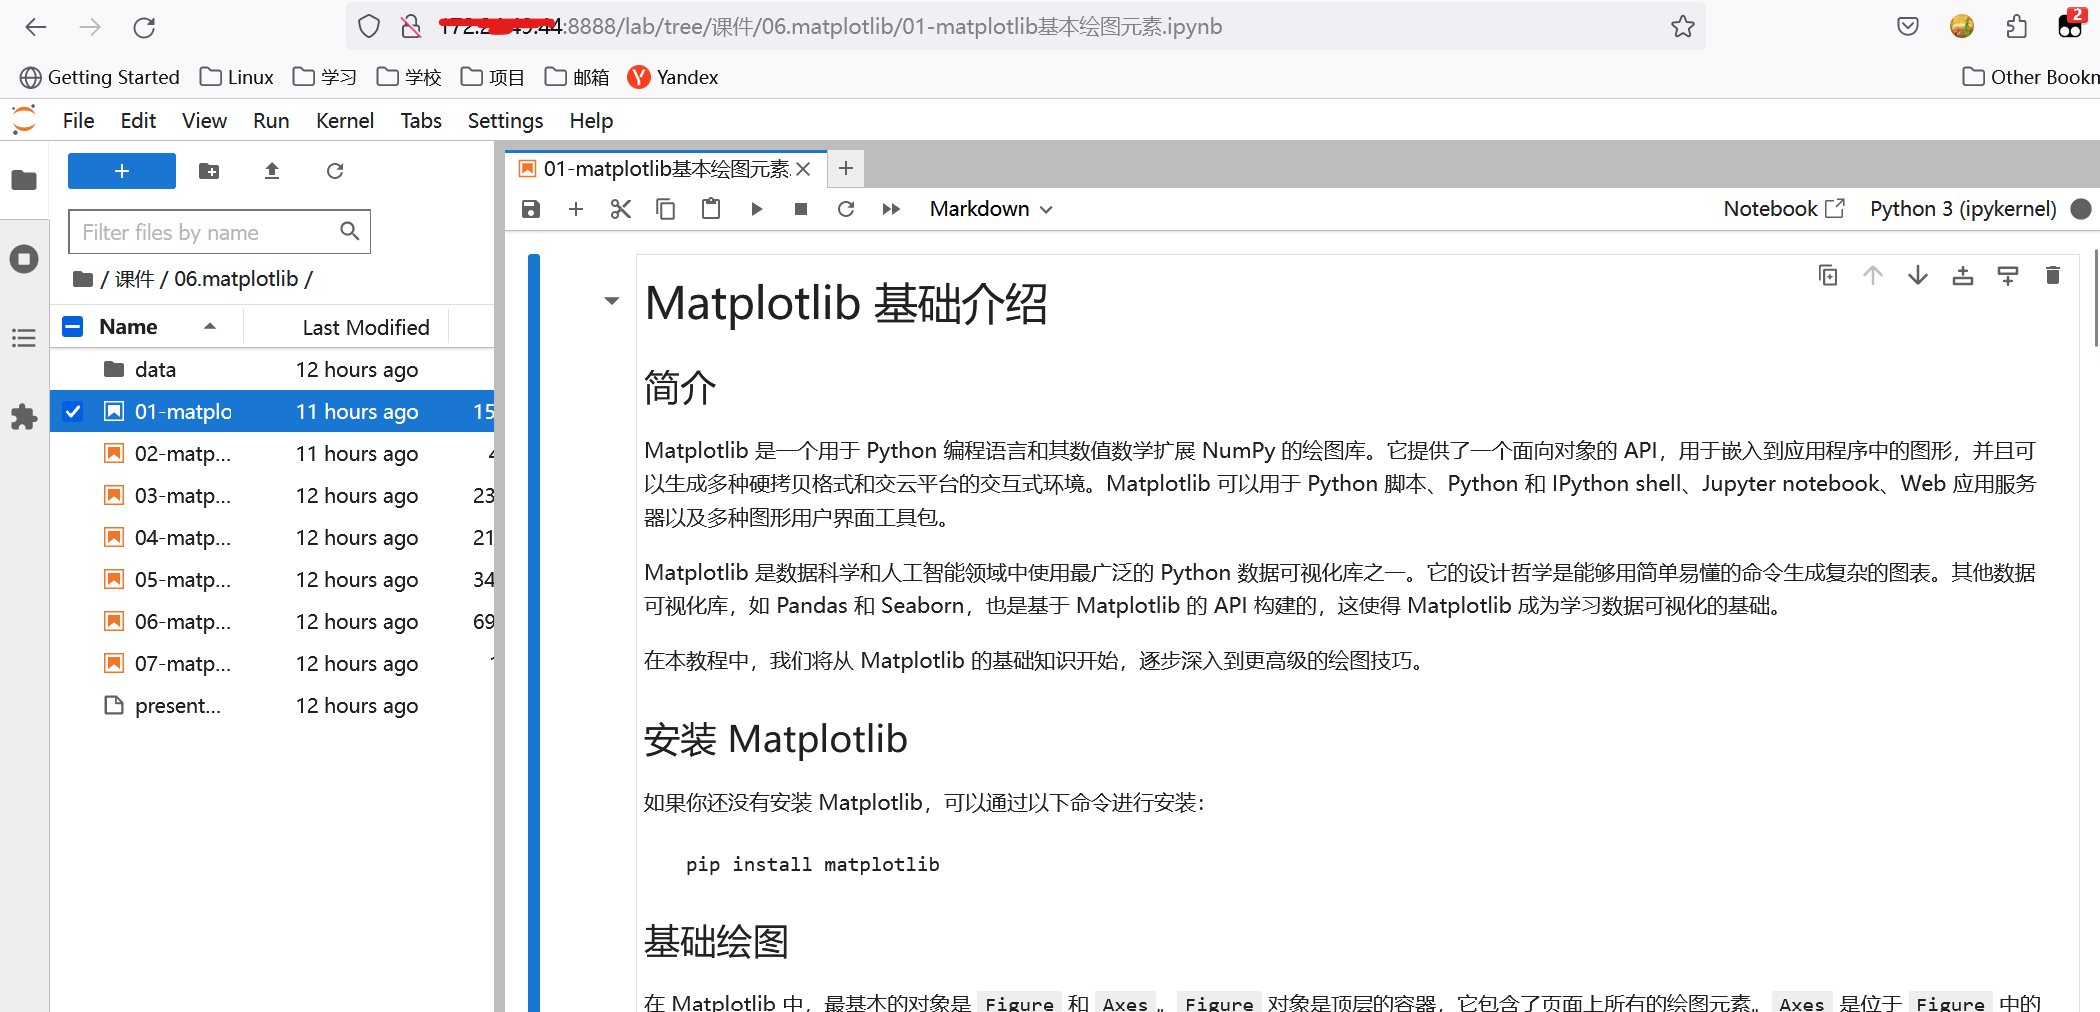
\includegraphics[width=.9\linewidth]{part/软件工程/环境搭建/JupyterNotbook/pic/Jupyternotebook概述/配置防火墙访问JupterLab.png}
    \caption{\label{fig:配置防火墙访问JupterLab}配置防火墙访问JupterLab}
\end{figure}

\subsubsubsection{SSH端口转发}
配置完需要使用ssh的端口转发(-L)功能，将远程的端口转发到本地(8080)，然后在本地访问即可,如图\ref{fig:访问远程JupterLab}所示。

\begin{lstlisting}[style=demostyle,numbers=none]
# ssh -L [本地端口]:localhost:[远程端口] [远程用户名]@[远程IP] -p [ssh连接端口]    
ssh -L 8080:localhost:8888 tony@192.168.1.119
\end{lstlisting}

\begin{figure}[htbp]
    \centering 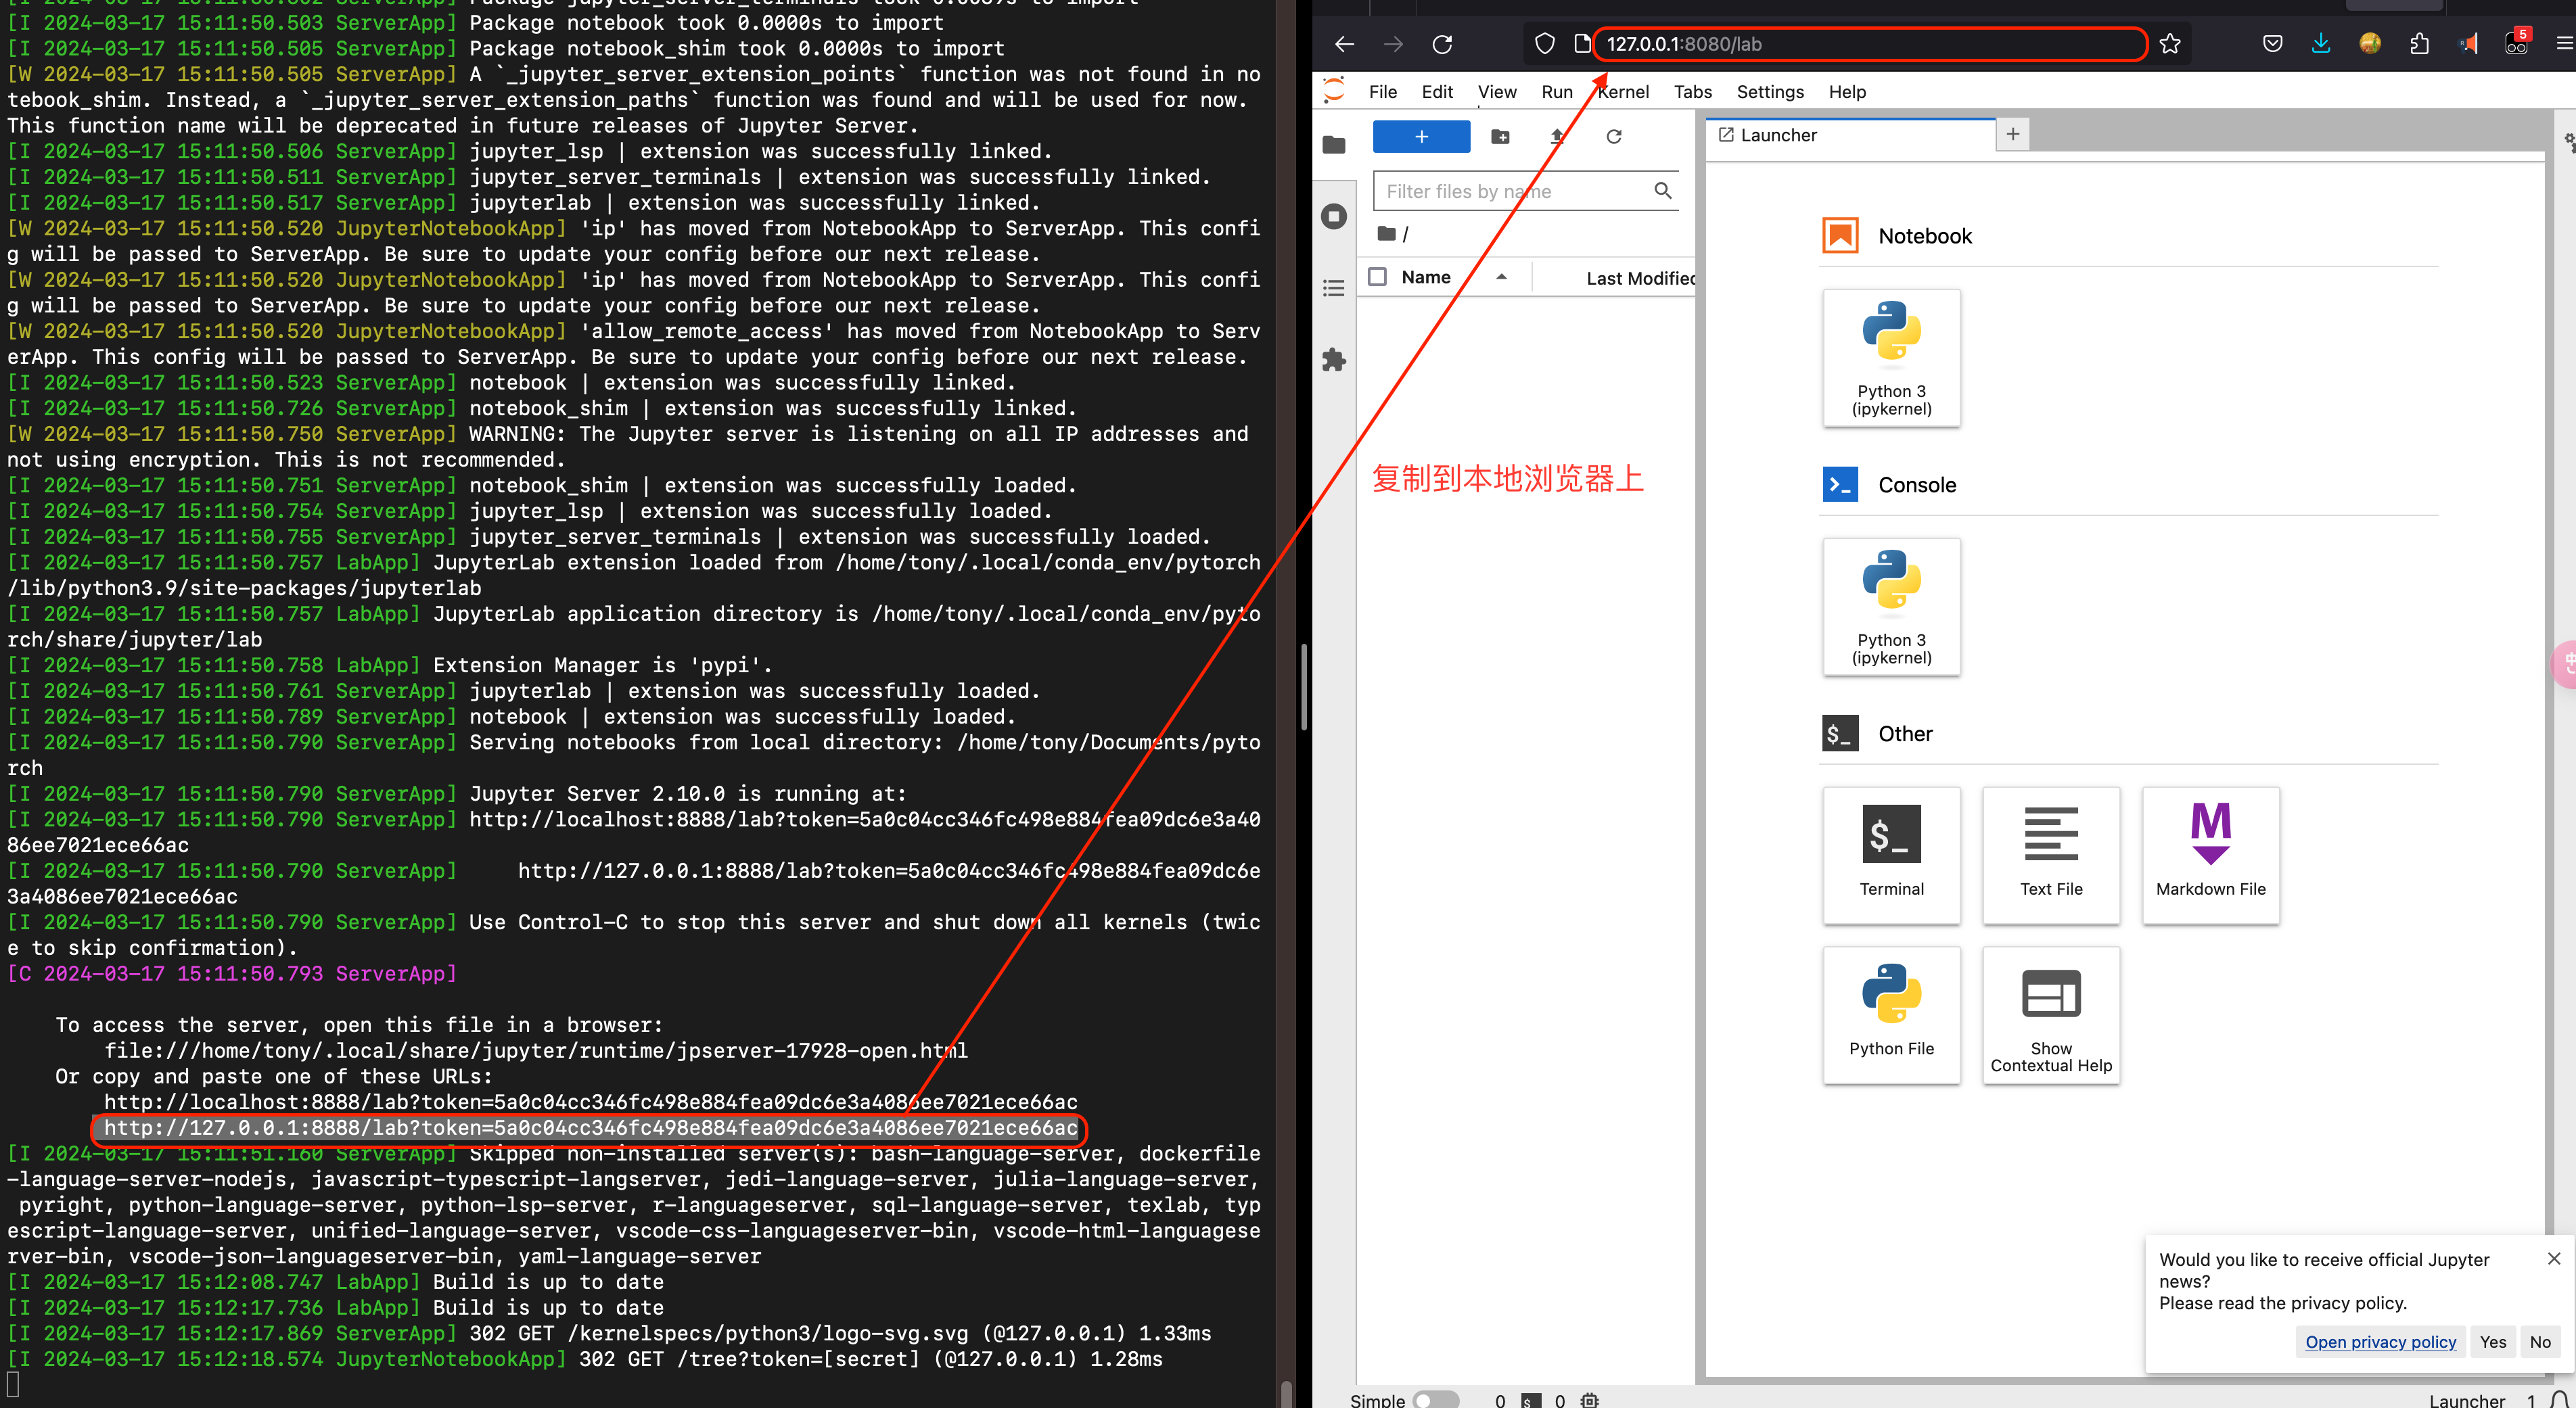
\includegraphics[width=.9\linewidth]{part/软件工程/环境搭建/JupyterNotbook/pic/Jupyternotebook概述/访问远程JupterLab.png}
      \caption{\label{fig:访问远程JupterLab}访问远程JupterLab,这里是localhost:8080}
\end{figure}

\subsubsubsection{配置密码}
按照如图\ref{fig:jupyterlab设置密码}所示设置密码。
\begin{figure}[htbp]
  \centering 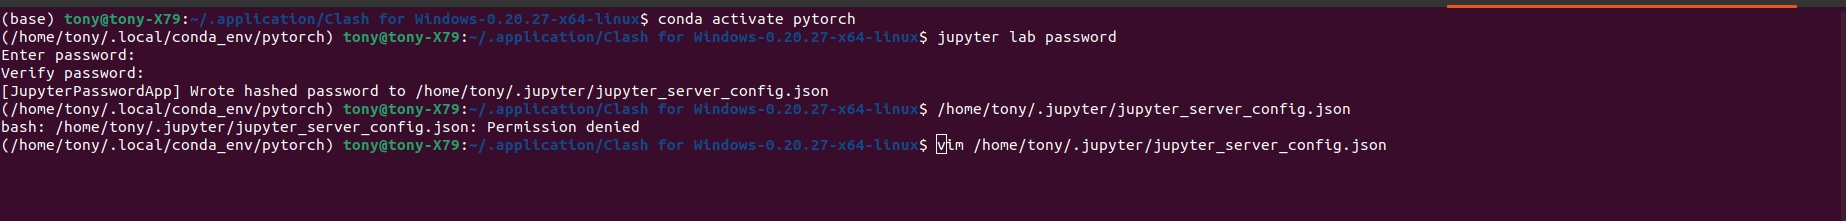
\includegraphics[width=.9\linewidth]{part/软件工程/环境搭建/JupyterNotbook/pic/Jupyternotebook概述/jupyterlab设置密码.png}
    \caption{\label{fig:jupyterlab设置密码}jupyterlab设置密码}
\end{figure}
然后按照如图\ref{fig:jupyterlab登入界面}所示登入。第一次登入需要输入密码，以后就不需要了。
\begin{figure}[htbp]
  \centering 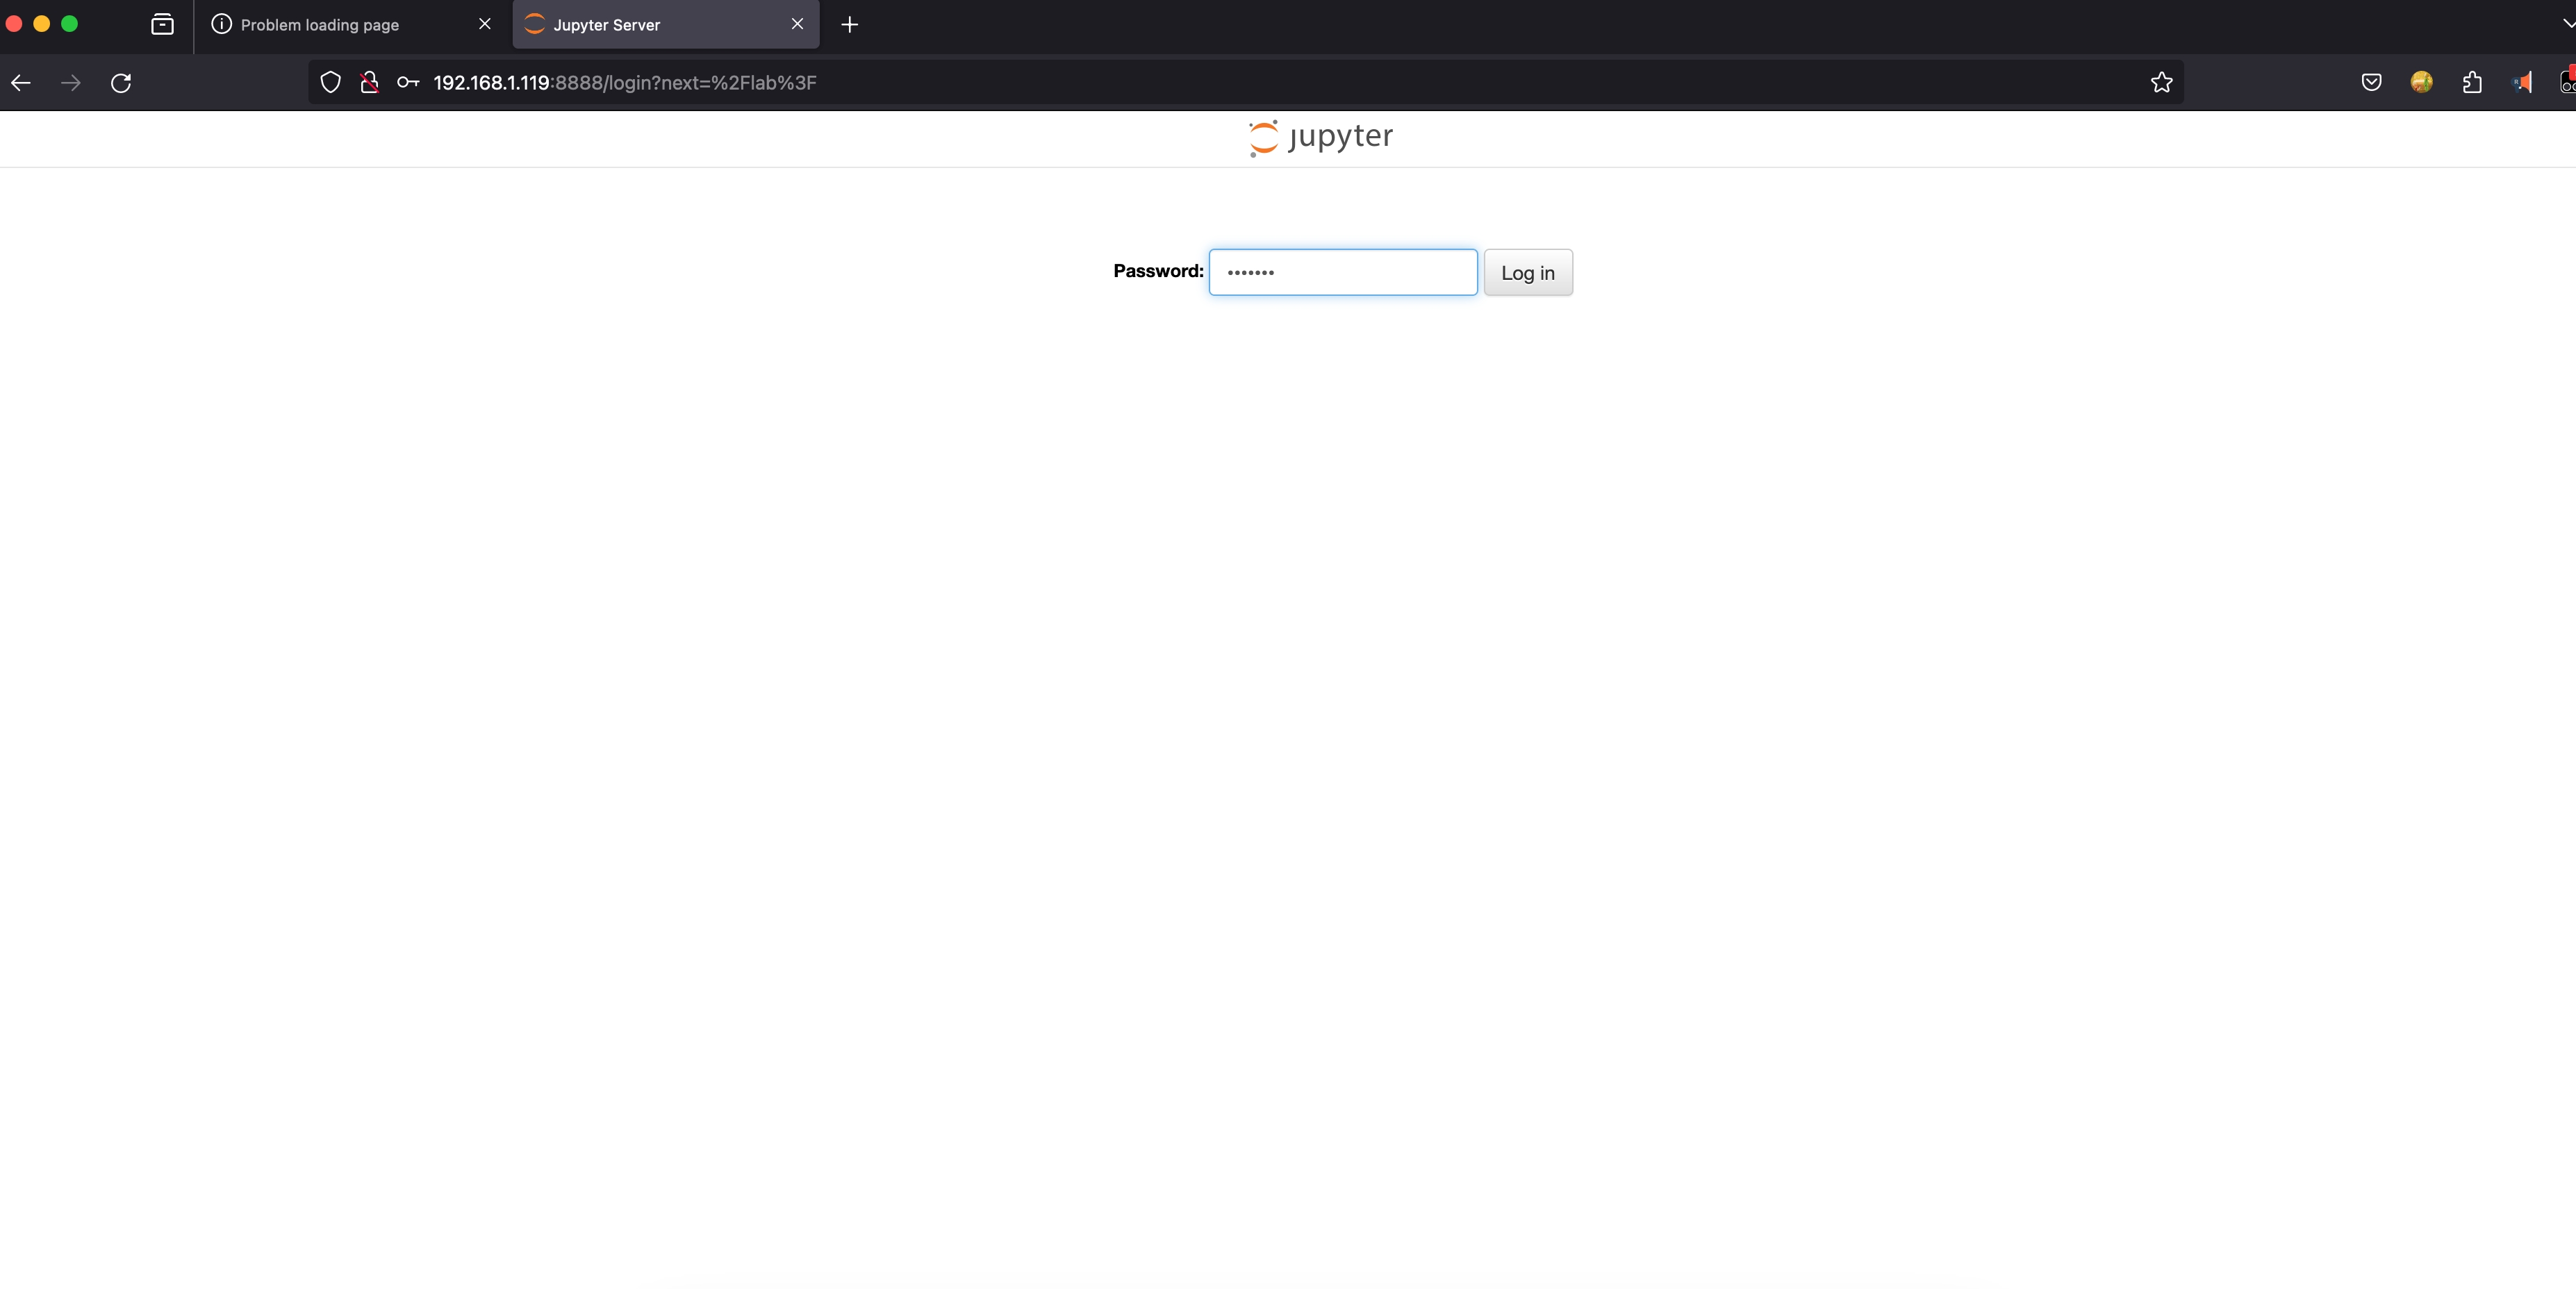
\includegraphics[width=.9\linewidth]{part/软件工程/环境搭建/JupyterNotbook/pic/Jupyternotebook概述/jupyterlab登入界面.png}
    \caption{\label{fig:jupyterlab登入界面}jupyterlab登入界面}
\end{figure}







\chapter{Jupter Notebook语法}
\section{JupyterLab的语法指令}
\subsection{writefile 写到一个文件}
\begin{lstlisting}[style=demostyle,numbers=none]
%%writefile 文件名
内容
\end{lstlisting}  

将当前cell的内容写入到文件中。

\begin{figure}[htpb]
  \centering
  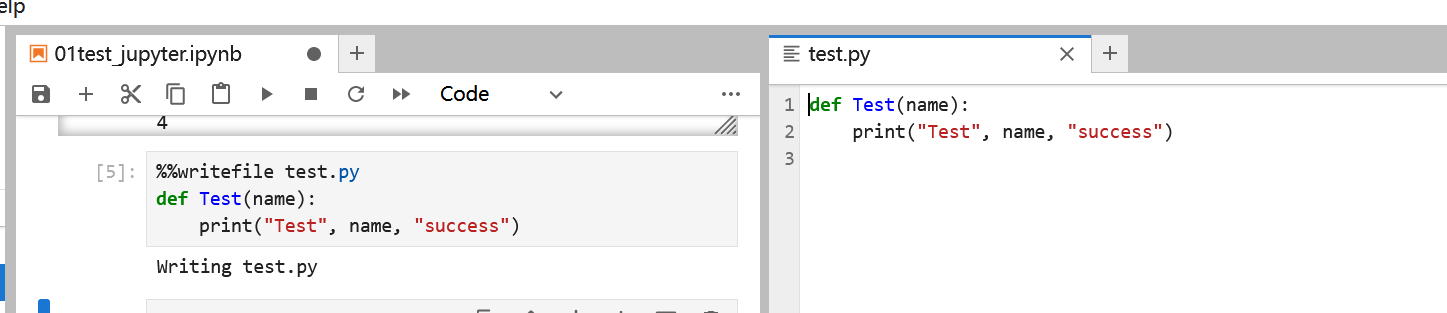
\includegraphics[width=0.6\textwidth]{part/软件工程/环境搭建/JupyterNotbook/pic/jupyternotebook语法/writefile指令.png}
  \caption{writefile指令}
  % \label{fig:writefile指令}
\end{figure}


\subsection{pycat 显示一个文件}
\begin{lstlisting}[style=demostyle,numbers=none]
%pycat 文件名
\end{lstlisting}

\begin{figure}[htpb]
  \centering
  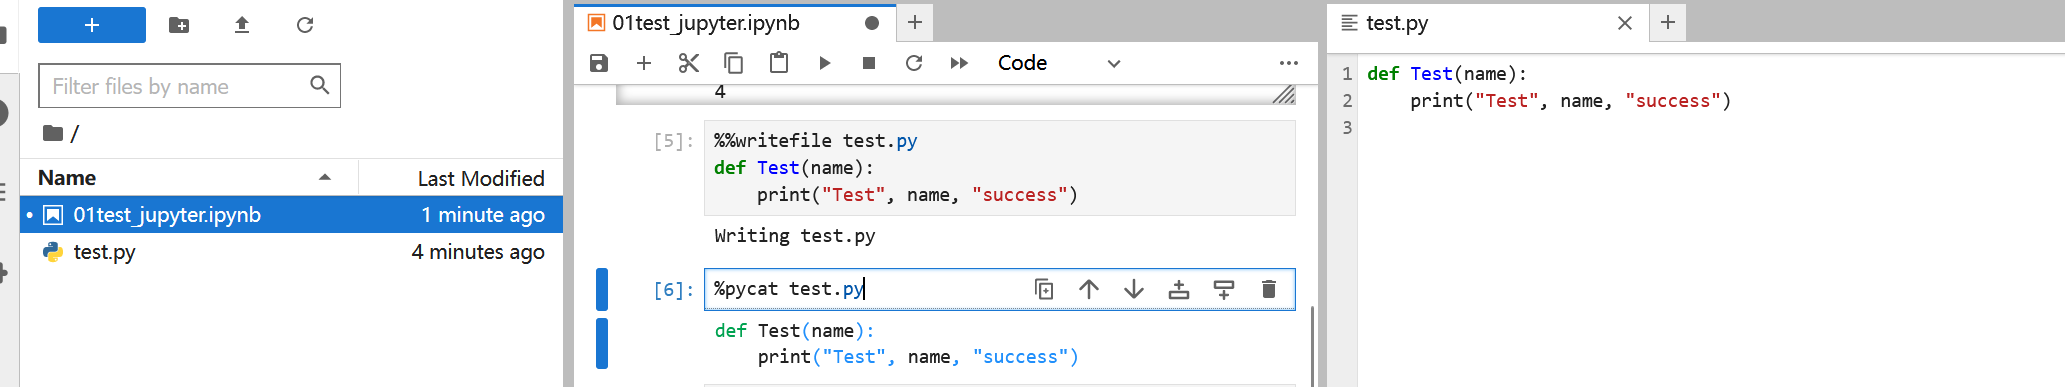
\includegraphics[width=0.6\textwidth]{part/软件工程/环境搭建/JupyterNotbook/pic/jupyternotebook语法/pycat指令.png}
  \caption{pycat指令}
  \label{fig:pycat指令}
\end{figure}


\subsection{run 执行一个文件}
\begin{lstlisting}[style=demostyle,numbers=none]
%run 文件名  
函数名(参数)
\end{lstlisting}

当然也可以通过\codeinline{import 文件名}导入文件,\codeinline{from 文件名 import 函数名}导入函数。

\begin{figure}[htpb]
  \centering
  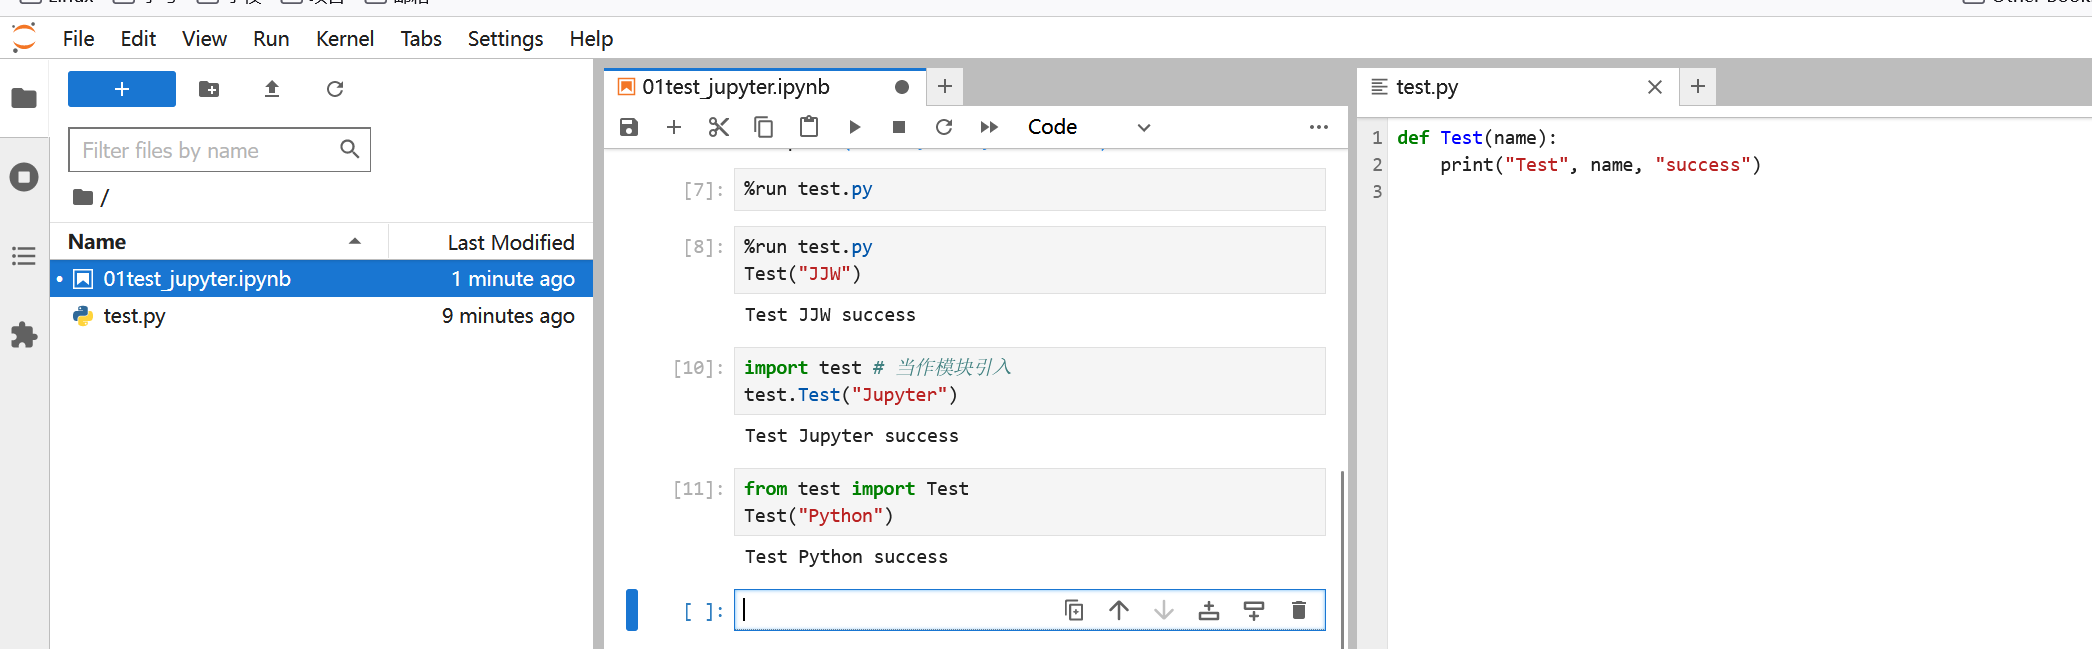
\includegraphics[width=0.6\textwidth]{part/软件工程/环境搭建/JupyterNotbook/pic/jupyternotebook语法/run指令.png}
  \caption{run指令}
  \label{fig:run指令}
\end{figure}

\subsection{计算代码运行时间}
多轮测试，取平均值。
\begin{lstlisting}[style=demostyle,numbers=none]
%timeit 函数名(参数) # 测试一条语句的运行时间

%%timeit # 测试一个cell的运行时间
\end{lstlisting}

只测试一次。
\begin{lstlisting}[style=demostyle,numbers=none]
%time 函数名(参数) # 测试一条语句的运行时间

%%time # 测试一个cell的运行时间
\end{lstlisting}

\begin{figure}[htpb]
  \centering
  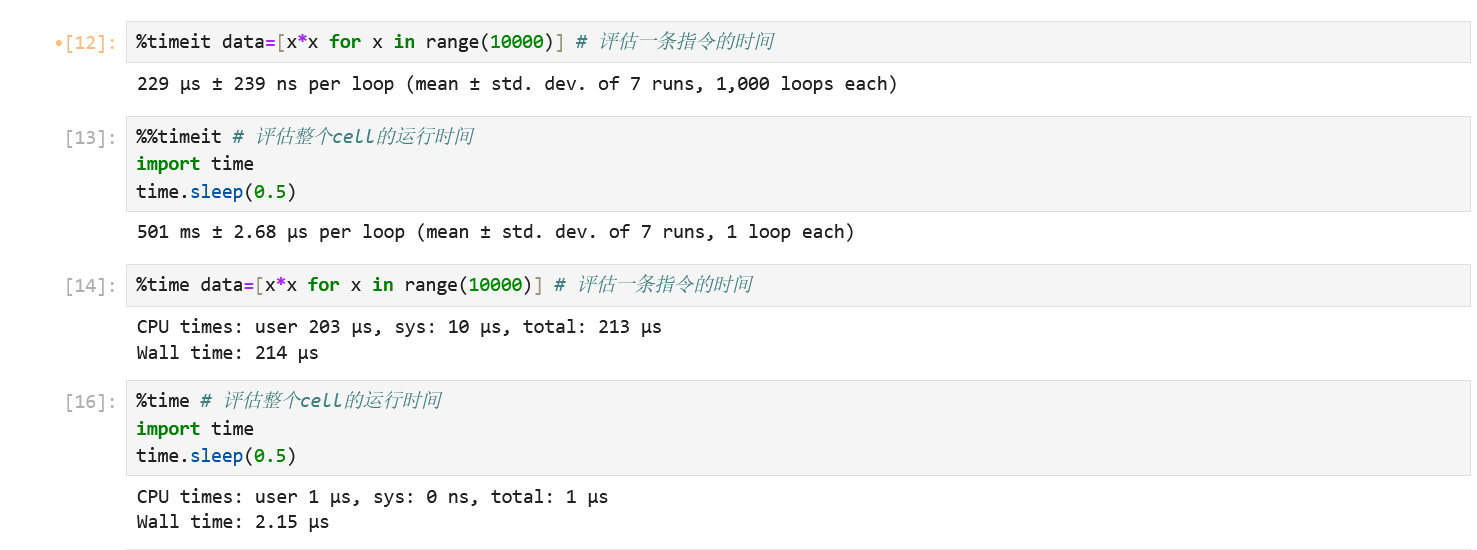
\includegraphics[width=0.6\textwidth]{part/软件工程/环境搭建/JupyterNotbook/pic/jupyternotebook语法/timeit和time指令.png}
  \caption{timeit和time指令}
  \label{fig:timeit和time指令}
\end{figure}

\subsection{whos 查看当前内存中的变量}
使用\codeinline{\%whos}或者\codeinline{\%who}查看当前内存中的变量。

包括定义的变量、函数、模块等。

\begin{figure}[htpb]
  \centering
  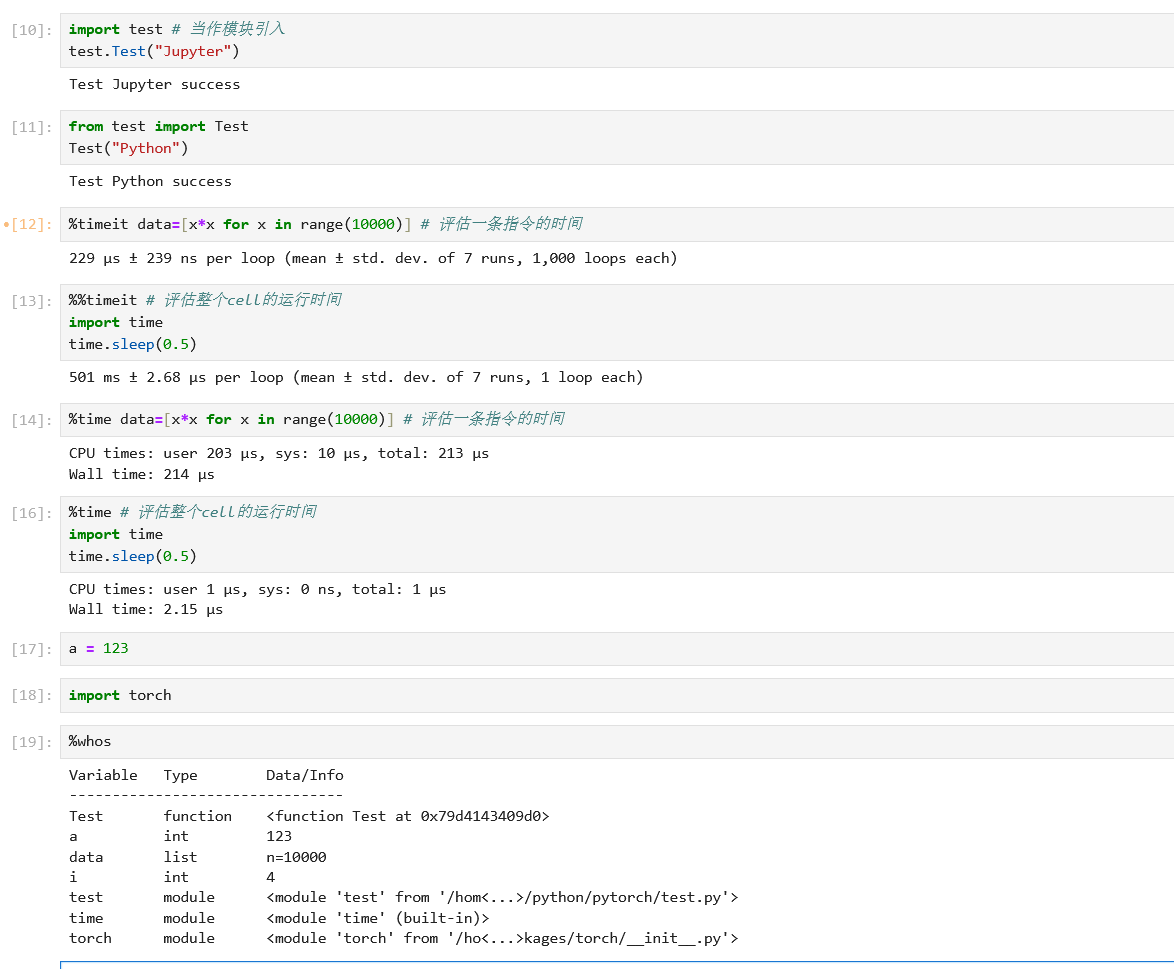
\includegraphics[width=0.8\textwidth]{part/软件工程/环境搭建/JupyterNotbook/pic/jupyternotebook语法/whos指令.png}
  \caption{whos指令}
  \label{fig:whos指令}
\end{figure}

\subsection{lsmagic 查看所有的魔法指令}
\begin{figure}[htpb]
  \centering
  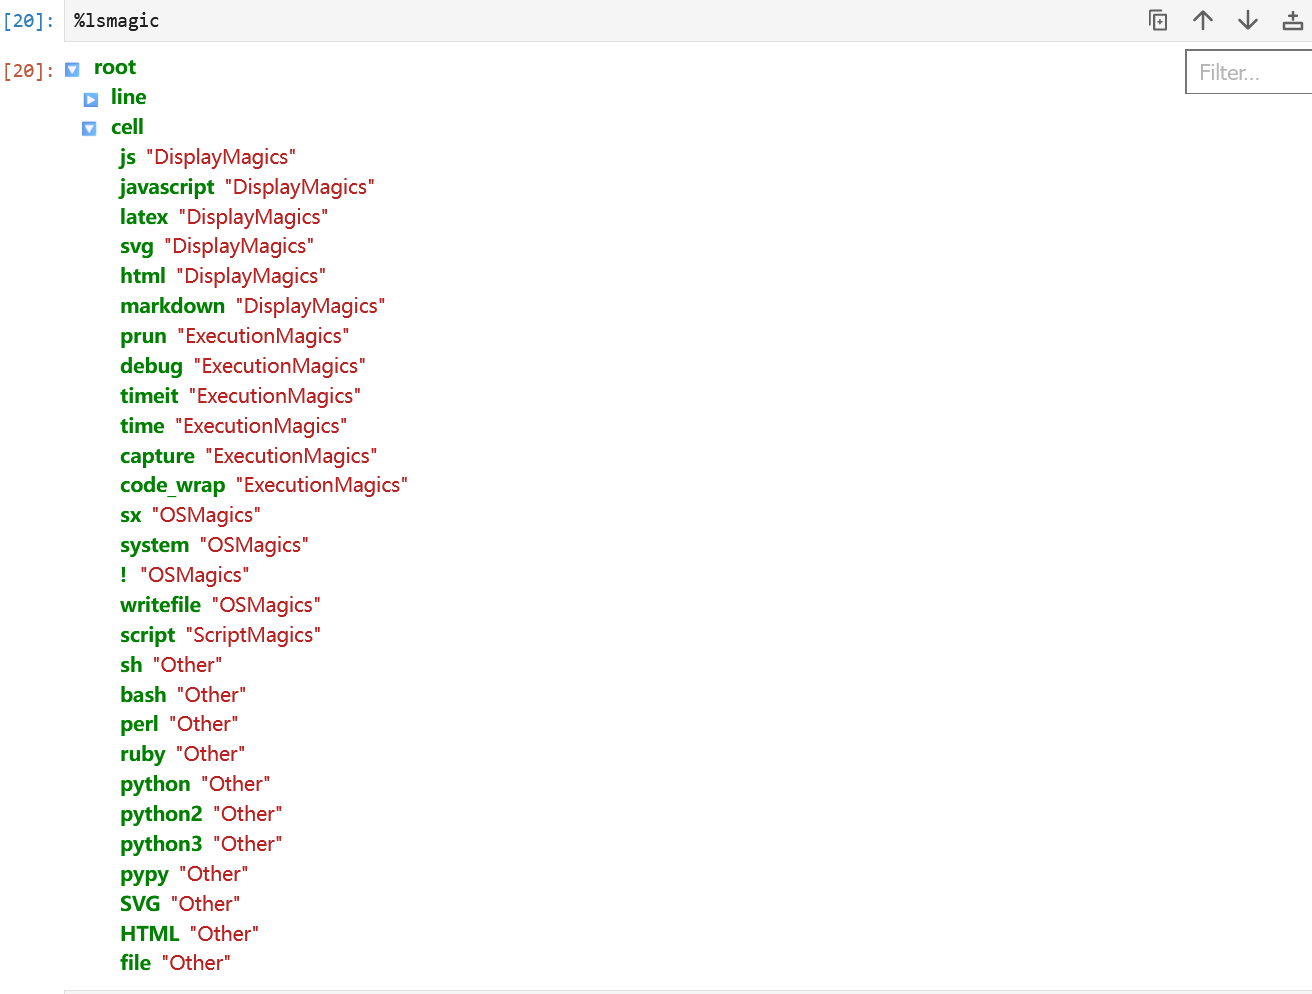
\includegraphics[width=0.8\textwidth]{part/软件工程/环境搭建/JupyterNotbook/pic/jupyternotebook语法/lsmagic指令.png}
  \caption{lsmagic指令}
  \label{fig:lsmagic指令}
\end{figure}






\chapter{自定义包}

\section{模块}
在 python 中，一个扩展名为 "\codeinline{.py}" 的文件称为一个\textcolor{blue}{\textbf{模块}} (module). 

模块可认为是一盒(箱)主题积木，
通过它可以拼出某一主题(某个系统、某个复杂求解问题)的东西。

与函数或类不同，一个函数或类相当于一块积木，而一个模块中可以包括很多函数或类.


\section{概述}
Python 中， "Package" 就是一个目录，
其中包括一组模块和一个"\codeinline{\_\_init\_\_.py}" 文件。
其中 \codeinline{\_\_init\_\_.py} 文件定义了包的属性和方法，
通常只是一个空文件，但是必须存在，\textcolor{red}{\textbf{切匆随意删除若删除}} \codeinline{\_\_init\_\_.py} 文件，
则该 Package 仅仅是一个目录，无法被导入或包含其他模型库和嵌套包.





\part{基本语法}
% 操作数
\chapter{操作数相关}
Python是弱类型语言, 变量的类型是根据赋值的值来决定的。

\section{概述}
变量是数据操作和数值计算的起始点，
算法用到的各种数据都是存储在变量内。

Python 是一门"弱类型"语言，所有的变量无须声明即可使用，变量的数据类型可以随时改变. 
Python3 中有六个标准的数据类型，分类如下:
\begin{enumerate}[label=\arabic*)]
    \item 不可变数据类型
    \begin{enumerate}[itemindent=1em,label=\arabic*)]
        \item Number (数字或数值)
        \item String (字符串)
        \item Thple(元组)
    \end{enumerate}
    
    
    \item 可变数据类型——序列
    \begin{enumerate}[itemindent=1em,label=\arabic*)]
        \item List (列表)
        \item Set (集合)
        \item Dictionary (字典)
    \end{enumerate}
\end{enumerate}

\subsection{标识符(变量名)}
\begin{enumerate}[label=\arabic*)]
    \item 第一个字符必须以字母(\codeinline{a-z}, \codeinline{A-Z})或下划线 \codeinline{\_} 。
    \item 标识符的其他的部分由字母、数字和下划线组成。
    \item 标识符对大小写敏感，count 和 Count 是不同的标识符。
    \item 标识符对长度无硬性限制，但建议保持简洁（一般不超过 20 个字符）。
    \item 禁止使用保留关键字，如 \codeinline{if}、\codeinline{for}、\codeinline{class} 等不能作为标识符。
\end{enumerate}
\begin{lstlisting}[style=demostyle,numbers=none]
# 合法标识符：    
age = 25
user_name = "Alice"
_total = 100
MAX_SIZE = 1024
calculate_area()
StudentInfo
__private_var

# 非法标识符：
2nd_place = "silver"    # 错误：以数字开头
user-name = "Bob"       # 错误：包含连字符
class = "Math"          # 错误：使用关键字
$price = 9.99          # 错误：包含特殊字符
for = "loop"           # 错误：使用关键字
\end{lstlisting}

Python 3 允许使用 Unicode 字符作为标识符，可以用中文作为变量名，非 ASCII 标识符也是允许的了。
\begin{lstlisting}[style=demostyle,numbers=none]
姓名 = "张三"  # 合法
π = 3.14159   # 合法
\end{lstlisting}
























\chapter{基本数据类型}

\section{Number——数字类型}
Python支持三种不同的 Number 数值类型:
\begin{enumerate}[label=\arabic*)]
    \item 整型 (int)：整数类型，表示没有小数部分的数字。
    \item 浮点型 (float)：浮点数类型，表示有小数部分的数字。
    \item 复数 (complex)：复数类型，表示实部和虚部
\end{enumerate}

如果需要对数据内置的类型进行转换，只需要将数据类型作为函数名即可，
如 \codeinline{int(x)} 转换为一个整数.

\subsection{int 整数类型}
\subsubsection{bool 布尔类型}
Python 中 bool 是 int 的子类(继承 \codeinline{int}),
故\codeinline{True==1}、 \codeinline{False==0}。

如要切实判断，则采用: \codeinline{XXX is True}.

\subsubsection{数字分隔符}
为了提高数字的的可读性, Python 3.x 允许使用下划线\codeinline{\_}作为数字（包括整数和小数）的分隔符。
通常每隔三个数字添加一个下划线, 类似于英文数字中的逗号。下划线不会影响数字本身的值。

\begin{lstlisting}[style=demostyle,numbers=none]
>>> 1_000_000
1000000
>>> click = 1_301_547
>>> distance = 384_000_000
>>> print("Python 教程阅读量：", click)
>>> print("地球和月球的距离：", distance)
Python 教程阅读量： 1301547
地球和月球的距离： 384000000
\end{lstlisting}

\subsection{float——浮点数(科学计数法)}
Python 3.x 支持科学计数法, 用\codeinline{e}或\codeinline{E}表示幂。
\begin{lstlisting}[style=demostyle,numbers=none]
>>> 1e6
1000000.0
>>> 1e-6
0.000001
>>> 1e+6
1000000.0
>>> 1e+0006
1000000.0
>>> 1e+0000006
1000000.0
>>> 2.1E5
210000.0
\end{lstlisting}

\subsubsection{浮点数精度问题}
Python 中浮点类型之间的运算, 其结果并不像我们想象的那样
\begin{lstlisting}[style=demostyle,numbers=none]
>>> 0.1+0.2
0.30000000000000004
>>> 0.1+0.1-0.2
0.0
>>> 0.1+0.1+0.1-0.3
5.551115123125783e-17
>>> 0.1+0.1+0.1-0.2
0.10000000000000003
\end{lstlisting}

如果需要非常精确的结果, 可以使用 \codeinline{decimal} 模块（其实就是别人开发好的程序, 我们可以直接拿来用）, 
它实现的十进制数运算适合会计方面的应用和有高精度要求的应用。例如：
\begin{lstlisting}[style=demostyle,numbers=none]
import decimal
a = decimal.Decimal("10.0")
b = decimal.Decimal("3")
print(10.0/3)
print(a/b)
\end{lstlisting}
\begin{lstlisting}[style=demostyle,numbers=none]
3.3333333333333335
3.333333333333333333333333333
\end{lstlisting}

如果 \codeinline{decimal} 模块还是无法满足需求, 还可以使用 \codeinline{fractions} 模块, 例如：
\begin{lstlisting}[style=demostyle,numbers=none]
>>> from fractions import Fraction
>>> a = Fraction(1, 3)
>>> b = Fraction(1, 3)
>>> a + b
Fraction(2, 3)
>>> a - b
Fraction(0, 3)
>>> a * b
Fraction(1, 9)
>>> a / b
Fraction(3, 1)
>>> print(Fraction(10,3))
10/3
\end{lstlisting}

\subsection{bool——布尔类型}
布尔类型包含
\begin{enumerate}[label=\arabic*)]
    \item \codeinline{True}: 真
    \item \codeinline{False}: 假
\end{enumerate}


\subsection{complex——复数类型}


% \section{String——字符串类型}
% 用引号括起的都是字符串，其中的引号可以是单引号，也可以是双引号
% \begin{lstlisting}[style=pythonstyle]
% "This is a string." 
% 'This is also a string.'
% \end{lstlisting}  

% \subsection{修改字符串的大小写}
% Python 提供了多种方法用于调整字符串的大小写格式：
% \begin{lstlisting}[style=pythonstyle]
% s = "This is a string."
% print(s.upper())   # 转换为大写
% print(s.lower())   # 转换为小写
% print(s.title())   # 转换为标题格式：每个单词首字母大写
% print(s.capitalize())  # 首字母大写，其余小写
% print(s.swapcase())    # 大小写互换
% \end{lstlisting}
% \begin{lstlisting}[style=demostyle,numbers=none]
% THIS IS A STRING.
% this is a string.
% This Is A String.
% This is a string.
% tHIS IS A STRING.
% \end{lstlisting}    

% \subsection{字符串拼接与重复}
% 可使用 \codeinline{+} 和 \codeinline{*} 运算符进行字符串连接和重复：
% \begin{lstlisting}[style=pythonstyle]
% s = "This is a string."
% print(s + " I am a Python programmer.")  # 拼接
% print(s * 2)                             # 重复
% \end{lstlisting}
% \begin{lstlisting}[style=demostyle,numbers=none]
% This is a string. I am a Python programmer.
% This is a string.This is a string.
% \end{lstlisting}

% \subsection{join：连接字符串}
% \begin{lstlisting}[style=pythonstyle]
% s = "apple,banana,cherry"
% print('-'.join(['a', 'b', 'c']))   # a-b-c
% \end{lstlisting}
% \begin{lstlisting}[style=demostyle,numbers=none]
% a-b-c
% \end{lstlisting}    



% \subsection{成员判断：in 与 not in}
% 用于检测子字符串是否存在于字符串中，返回布尔值：
% \begin{lstlisting}[style=pythonstyle]
% s = "This is a string."
% print("string" in s)        # True
% print("Python" not in s)    # True
% \end{lstlisting}

% \subsection{成员类型判断}
% \begin{enumerate}[label=\arabic*)]
%     \item \codeinline{str.isalpha()}: 字符串只包含字母
%     \item \codeinline{str.isdigit()}: 字符串只包含数字
%     \item \codeinline{str.isalnum()}: 字符串只包含字母或数字
% \end{enumerate}
% \begin{lstlisting}[style=pythonstyle]
% print("123".isdigit())             # True
% print("Hello".isalpha())           # True
% print("Hello123".isalnum())        # True
% \end{lstlisting}

% \subsection{字符串替换}
% 使用 \codeinline{str.replace(old, new[, count])} 方法替换子串：
% \begin{lstlisting}[style=pythonstyle]
% s = "This is a string."
% print(s.replace("string", "sentence"))      # 全部替换
% print(s.replace("i", "I", 2))               # 最多替换前2次出现
% \end{lstlisting}
% \begin{lstlisting}[style=demostyle,numbers=none]
% This is a sentence.
% ThIs Is a string.
% \end{lstlisting}

% \subsection{删除字符串两端或指定字符}
% Python 提供多种去除空白或指定字符的方法：
% \begin{lstlisting}[style=pythonstyle]
% s = "   Hello, World!   "
% print(s.strip())        # 去除首尾空白（包括空格、\n、\t等）
% print(s.lstrip())       # 去除左侧空白
% print(s.rstrip())       # 去除右侧空白

% # 可指定要去除的字符
% t = "###Hello###"
% print(t.strip('#'))     # 输出: Hello
% \end{lstlisting}
% \begin{lstlisting}[style=demostyle,numbers=none]
% Hello, World!
% Hello, World!   
%    Hello, World!
% Hello
% \end{lstlisting}

% \subsection{子串}
% \subsubsection{索引与切片}
% 使用 \codeinline{str.split([sep[, maxsplit]]) } 方法将字符串拆分为子字符串：
% \begin{lstlisting}[style=pythonstyle]
% s = "apple,banana,cherry"
% print(s.split(','))                # ['apple', 'banana', 'cherry']
% \end{lstlisting}
% \begin{lstlisting}[style=demostyle,numbers=none]
% ['apple', 'banana', 'cherry']
% \end{lstlisting}   

% \begin{lstlisting}[style=pythonstyle]
% s = "Python"

% # 索引：获取单个字符
% print(s[0])      # 'P'         （正向索引从0开始）
% print(s[-1])     # 'n'         （反向索引从-1开始）

% # 切片：获取子串 [start:end:step]
% print(s[1:4])    # 'yth'       （包含start，不包含end）
% print(s[:3])     # 'Pyt'       （省略start表示从开头）
% print(s[3:])     # 'hon'       （省略end表示到末尾）
% print(s[::2])    # 'Pto'       （步长为2）
% print(s[::-1])   # 'nohtyP'    （反转字符串）
% \end{lstlisting}
% \begin{lstlisting}[style=demostyle,numbers=none]
% P
% n
% yth
% Pyt
% hon
% Pto
% nohtyP
% \end{lstlisting}

% \subsubsection{find与index:查找子串位置}
% \begin{lstlisting}[style=pythonstyle]
% s = "This is a string."
% print(s.find("is"))      # 2
% print(s.index("is"))     # 2
% print(s.find("Python"))  # -1
% \end{lstlisting}












\section{类型转换}
\subsection{type}
\begin{lstlisting}[style=demostyle,numbers=none]
Python 3.9.19 (main, Mar 21 2024, 17:11:28)
[GCC 11.2.0] :: Anaconda, Inc. on linux
Type "help", "copyright", "credits" or "license" for more information.
>>> type(8)
<class 'int'>
>>> type("8")
<class 'str'>
>>> type(False)
<class 'bool'>
>>> type(true)
Traceback (most recent call last):
  File "<stdin>", line 1, in <module>
NameError: name 'true' is not defined
>>> num = 20 + 15j
>>> type(num)
<class 'complex'>
\end{lstlisting}

\subsection{显式类型转换}
\begin{lstlisting}[style=demostyle,numbers=none]
>>> int("8") # 将字符串转换为整数
8
>>> float("8")
8.0
>>> str(8) # 将整数转换为字符串
'8'
>>> bool(8) # 将整数转换为布尔值
True
>>> bool(0)
False
\end{lstlisting}

\section{缓存重用机制}
Python 缓冲机制是为提高程序执行的效率服务的, 实际上就是在 Python 解释器启动时从内存空间中开辟出一小部分, 
用来存储高频使用的数据, 这样可以大大减少高频使用的数据创建时申请内存和销毁时撤销内存的开销。

\begin{table}[htpb]
\begin{tabular}{|l|ll|}
\hline
\multicolumn{1}{|c|}{\textbf{数据类型}} & \multicolumn{1}{c|}{\textbf{是否可以重用}}                              & \multicolumn{1}{c|}{\textbf{生效范围}} \\ \hline
范围在 {[}-5, 256{]} 之间的小整数            & \multicolumn{1}{l|}{\multirow{3}{*}{如果之前在程序中创建过, 就直接存入缓存, 后续不再创建。}} & \multirow{3}{*}{全局}                \\ \cline{1-1}
bool 类型                             & \multicolumn{1}{l|}{}                                             &                                    \\ \cline{1-1}
字符串类型数据                             & \multicolumn{1}{l|}{}                                             &                                    \\ \hline
大于 256 的整数                          & \multicolumn{1}{l|}{\multirow{2}{*}{只要在本代码块内创建过, 就直接缓存, 后续不再创建。}}   & \multirow{2}{*}{本代码块}              \\ \cline{1-1}
大于 0 的浮点型小数                         & \multicolumn{1}{l|}{}                                             &                                    \\ \hline
小于 0 的浮点型小数                         & \multicolumn{2}{l|}{\multirow{2}{*}{不进行缓存, 每次都需要额外创建。}}                                                 \\ \cline{1-1}
小于 -5 的整数                           & \multicolumn{2}{l|}{}                                                                                  \\ \hline
\end{tabular}
\caption{缓存重用机制}
\end{table}

\begin{lstlisting}[style=pythonstyle]
#范围在 [-5, 256] 之间的小整数
int1 = -5
int2 = -5
print("[-5, 256] 情况下的两个变量：", id(int1), id(int2))
#bool 类型
bool1 = True
bool2 = True
print("bool 类型情况下的两个变量：",id(bool1),id(bool2))

#对于字符串
s1 = "3344"
s2 = "3344"
print("字符串情况下的两个交量", id(s1), id(s2))
#大于 256 的整数
int3 = 257
int4 = 257
print("大于 256 的整数情况下的两个变量", id(int3), id(int4))
#大于 0 的浮点数
f1 = 256.4
f2 = 256.4
print("大于 0 的浮点数情况下的两个变量", id(f1), id(f2))
#小于 0 的浮点数
f3 = -2.45
f4 = -2.45
print("小于 0 的浮点数情况下的两个变量", id(f3), id(f4))
#小于 -5 的整数
n1 = -6
n2 = -6
print("小于 -5 的整数情况下的两个变量", id(n1), id(n2))
\end{lstlisting}
\begin{lstlisting}[style=demostyle,numbers=none]
[-5, 256] 情况下的两个变量： 2169665579120 2169665579120
bool 类型情况下的两个变量： 140731067889768 140731067889768
字符串情况下的两个交量 2169668343408 2169668343408
大于 256 的整数情况下的两个变量 2169668069648 2169668069648
大于 0 的浮点数情况下的两个变量 2169666229936 2169666229936
小于 0 的浮点数情况下的两个变量 2169668070320 2169668070320
小于 -5 的整数情况下的两个变量 2169668070032 2169668070032
\end{lstlisting}

\begin{lstlisting}[style=pythonstyle]
def fun():
    #[-5,256]
    int1 = -5
    int2 = -5
    print("fun 中 -5 的存储状态",id(int1), id(int2))

    #bool 类型
    bool2 = True
    bool3 = True
    print("fun 中 bool 类型的存储状态",id(bool3),id(bool2))

    #字符串类型
    s1 = "3344"
    s2 = "3344"
    print("fun 中 3344 字符串的存储状态", id(s1), id(s2))

    #大于 256
    int3 = 257
    int4 = 257
    print("fun 中 257 的存储状态", id(int3), id(int4))

    #浮点类型
    f1 = 256.4
    f2 = 256.4
    print("fun 中 256.4 的存储状态",id(f1), id(f2))

    #小于 -5
    n1 = -6
    n2 = -6
    print("fun 中 -6 的存储状态", id(n1), id(n2))
 
fun()
\end{lstlisting}
\begin{lstlisting}[style=demostyle,numbers=none]
fun 中 -5 的存储状态 2022312994928 2022312994928
fun 中 bool 类型的存储状态 140731067889768 140731067889768
fun 中 3344 字符串的存储状态 2022319364656 2022319364656
fun 中 257 的存储状态 2022319089936 2022319089936
fun 中 256.4 的存储状态 2022313645744 2022313645744
fun 中 -6 的存储状态 2022319090032 2022319090032
\end{lstlisting}

\chapter{[序列] 数据结构}
\section{序列}
\textcolor{blue}{\textbf{序列}}: 一块可存放多个值的连续内存空间，这些值按一定顺序排列，可通过每个值所在位置的编号（称为索引）访问它们。

\subsection{序列内置函数}
下面的函数适用于所有序列类型，包括字符串、列表、元组等。

\subsubsection{len 序列的长度}

\begin{enumerate}[label=\arabic*)]
    \item 字符串
\begin{lstlisting}[style=demostyle,numbers=none]
chinese_zodiac = "鼠牛虎兔龙蛇马羊猴鸡狗猪"
print(len(chinese_zodiac))
>>> 12
\end{lstlisting}

    \item 列表
\begin{lstlisting}[style=demostyle,numbers=none]
name = ['张三', '李四', '王五']
print(len(name))
>> 3
\end{lstlisting}

    \item 元组
\begin{lstlisting}[style=demostyle,numbers=none]
name = ('张三', '李四', '王五')
print(len(name))
>> 3
\end{lstlisting}

    \item 字典
\begin{lstlisting}[style=demostyle,numbers=none]
name = {'name': '张三', 'age': 18}
print(len(name))
>> 2
\end{lstlisting}

    \item 集合
\begin{lstlisting}[style=demostyle,numbers=none]
name = {'张三', '李四', '王五'}
print(len(name))
>> 3
\end{lstlisting}
\end{enumerate}


\subsubsection{max 序列的最大值}

\begin{enumerate}[label=\arabic*)]
    \item 字符串
\begin{lstlisting}[style=demostyle,numbers=none]
chinese_zodiac = "鼠牛虎兔龙蛇马羊猴鸡狗猪"
print(max(chinese_zodiac))
>>> 龙

my_string = "hello"
print(max(my_string))  # 输出: 'o'
>>> o
\end{lstlisting}

    \item 列表
\begin{lstlisting}[style=demostyle,numbers=none]
name = ['张三', '李四', '王五']
print(max(name))
>>> 王五

my_list = [1, 2, 3, 4, 5]
print(max(my_list))  # 输出: 5
>>> 5
\end{lstlisting}

    \item 元组
\begin{lstlisting}[style=demostyle,numbers=none]
name = ('张三', '李四', '王五')
print(max(name))
>>> 王五

my_tuple = (1, 2, 3)
print(max(my_tuple))  # 输出: 3
>>> 3
\end{lstlisting}

    \item 字典
\begin{lstlisting}[style=demostyle,numbers=none]
my_dict = {'a': 1, 'b': 2, 'c': 3}
print(max(my_dict))  # 输出: ('c', 3)
>>> c
print(max(my_dict.values()))
>>> 3
\end{lstlisting}

    \item 集合
\begin{lstlisting}[style=demostyle,numbers=none]
my_set = {1, 2, 3, 4}
print(max(my_set))  # 输出: 4
>>> 4
\end{lstlisting}
\end{enumerate}


\subsubsection{min 序列的最小值}
\begin{enumerate}[label=\arabic*)]
    \item 字符串
\begin{lstlisting}[style=demostyle,numbers=none]
chinese_zodiac = "鼠牛虎兔龙蛇马羊猴鸡狗猪"
print(min(chinese_zodiac))  # 输出: '鼠'
>>> 鼠
\end{lstlisting}

    \item 列表
\begin{lstlisting}[style=demostyle,numbers=none]
name = ['张三', '李四', '王五']
print(min(name))  # 输出: '张三'
>>> 张三
\end{lstlisting}

    \item 元组
\begin{lstlisting}[style=demostyle,numbers=none]
name = ('张三', '李四', '王五')
print(min(name))  # 输出: '张三'
>>> 张三
\end{lstlisting}

    \item 字典
\begin{lstlisting}[style=demostyle,numbers=none]
my_dict = {'a': 1, 'b': 2, 'c': 3}
print(min(my_dict))  # 输出: ('a', 1)
>>> a
print(min(my_dict.values()))
>>> 1
\end{lstlisting}

    \item 集合
\begin{lstlisting}[style=demostyle,numbers=none]
my_set = {1, 2, 3, 4}
print(min(my_set))  # 输出: 1
>>> 1
\end{lstlisting}

\end{enumerate}


\subsubsection{sum 返回序列的和}
\begin{enumerate}[label=\arabic*)]
    \item 字符串

    字符串不能使用 \codeinline{sum} 函数。

    \item 列表
\begin{lstlisting}[style=demostyle,numbers=none]
my_list = [1, 2, 3, 4, 5]
print(sum(my_list))  # 输出: 15
\end{lstlisting}

    \item 元组
\begin{lstlisting}[style=demostyle,numbers=none]
my_tuple = (1, 2, 3)
print(sum(my_tuple))  # 输出: 6
\end{lstlisting}

    \item 字典

    字典只能对值进行求和。
\begin{lstlisting}[style=demostyle,numbers=none]
# 字典（需要对值进行求和）
my_dict = {'a': 1, 'b': 2, 'c': 3}
print(sum(my_dict.values()))  # 输出: 6
\end{lstlisting}
    \item 集合

\begin{lstlisting}[style=demostyle,numbers=none]
my_set = {1, 2, 3, 4}
print(sum(my_set))  # 输出: 10
\end{lstlisting}
    
\end{enumerate}


\subsubsection{sorted 返回排序后的序列}
\begin{enumerate}[label=\arabic*)]
    \item 字符串
\begin{lstlisting}[style=demostyle,numbers=none]
my_string = "cba"
print(sorted(my_string))  
>>> ['a', 'b', 'c']
\end{lstlisting}

    \item 列表
\begin{lstlisting}[style=demostyle,numbers=none]
my_list = [3, 1, 4, 1, 5]
print(sorted(my_list))  
>>> [1, 1, 3, 4, 5]
\end{lstlisting}

    \item 元组（排序后转为列表）
\begin{lstlisting}[style=demostyle,numbers=none]
my_tuple = (3, 1, 4, 1, 5)
print(sorted(my_tuple))  
>>> [1, 1, 3, 4, 5]
\end{lstlisting}

    \item 字典（按键排序）
\begin{lstlisting}[style=demostyle,numbers=none]
my_dict = {'b': 2, 'a': 1, 'c': 3}
print(sorted(my_dict))
>>> ['a', 'b', 'c']
\end{lstlisting}

    \item 集合（排序后转为列表）
\begin{lstlisting}[style=demostyle,numbers=none]
my_set = {3, 1, 4}
print(sorted(my_set))
>>> [1, 3, 4]
\end{lstlisting}
\end{enumerate}

\subsubsection{reversed 返回逆序的序列}
\begin{enumerate}[label=\arabic*)]
    \item 字符串
\begin{lstlisting}[style=demostyle,numbers=none]
my_string = "hello"
print(''.join(reversed(my_string)))  # 输出: "olleh"
>>> olleh
\end{lstlisting}

    \item 列表
\begin{lstlisting}[style=demostyle,numbers=none]
my_list = [1, 2, 3, 4, 5]
print(list(reversed(my_list)))  # 输出: [5, 4, 3, 2, 1]
>>> [5, 4, 3, 2, 1]
\end{lstlisting}

    \item 元组
\begin{lstlisting}[style=demostyle,numbers=none]
my_tuple = (1, 2, 3, 4, 5)
print(tuple(reversed(my_tuple)))  # 输出: (5, 4, 3, 2, 1)
>>> (5, 4, 3, 2, 1)
\end{lstlisting}

    \item 字典（不能直接逆序，但可以逆序键或值）
\begin{lstlisting}[style=demostyle,numbers=none]
my_dict = {'a': 1, 'b': 2, 'c': 3}
print(list(reversed(my_dict)))  # 输出: ['c', 'b', 'a'] (逆序键)
>>> ['c', 'b', 'a']
\end{lstlisting}

    \item 集合

    集合是无序的，所以不能使用 \codeinline{reversed} 函数。
\end{enumerate}


\subsubsection{enumerate 返回索引和元素组成的元组}
\begin{enumerate}[label=\arabic*)]
    \item 字符串

    字符串不能使用 \codeinline{enumerate} 函数。

    \item 列表
\begin{lstlisting}[style=demostyle,numbers=none]
>>> my_list = ['a', 'b', 'c']
>>> for index, value in enumerate(my_list):
...     print(index, value)
...
0 a
1 b
2 c
\end{lstlisting}

    \item 元组
\begin{lstlisting}[style=demostyle,numbers=none]
>>> my_tuple = ('a', 'b', 'c')
>>> for index, value in enumerate(my_tuple):
...     print(index, value)
...
0 a
1 b
2 c
\end{lstlisting}

    \item 字典

    字典不能使用 \codeinline{enumerate} 函数。

    \item 集合

    集合不能使用 \codeinline{enumerate} 函数。
\end{enumerate}


\subsection{序列的通用操作}

\subsubsection{[] 索引访问}

\begin{enumerate}[label=\arabic*)]
    \item 字符串
\begin{lstlisting}[style=demostyle,numbers=none]
>>> chinese_zodiac = "鼠牛虎兔龙蛇马羊猴鸡狗猪"
>>> print(chinese_zodiac[0])
鼠
>>> print(chinese_zodiac[0:4])
鼠牛虎兔
>>> print(chinese_zodiac[-1])
猪
>>> print(chinese_zodiac[-3:-1])
鸡狗
>>> print(chinese_zodiac[-3:])
鸡狗猪
>>> print(chinese_zodiac[0:-1:2])
鼠虎龙马猴狗
\end{lstlisting}

    \item 列表
\begin{lstlisting}[style=demostyle,numbers=none]
变量名 = [值1, 值2, 值3,...]

name = ['张三', '李四', '王五']
print(name[1])
>> 李四
\end{lstlisting}

    \item 元组
\begin{lstlisting}[style=demostyle,numbers=none]
变量名 = (值1, 值2, 值3,...)

name = ('张三', '李四', '王五')
print(name[1])
>> 李四
\end{lstlisting}

    \item 字典
\begin{lstlisting}[style=demostyle,numbers=none]
变量名 = {键1:值1, 键2:值2, 键3:值3,...}

name = {'name':'张三', 'age':18, 'sex':'男'}
print(name['name'])
>> 张三
\end{lstlisting}

    \item 集合
\begin{lstlisting}[style=demostyle,numbers=none]
变量名 = {值1, 值2, 值3,...}

name = {'张三', '李四', '王五'}
print(name[1])
>> 李四
\end{lstlisting}
\end{enumerate}

\subsubsection{index 查找元素的索引}
\begin{enumerate}[label=\arabic*)]
    \item 字符串

    字符串没有 \codeinline{index} 方法，但是可以使用 \codeinline{find} 方法。

\begin{lstlisting}[style=demostyle,numbers=none]
# 字符串
my_string = "Hello, World!"
index_of_world = my_string.find("World")  # 查找子字符串 "World" 的索引
print(index_of_world)  # 输出: 7

# 未找到时返回 -1
index_of_python = my_string.find("Python")
print(index_of_python)  # 输出: -1
\end{lstlisting}

    \item 列表
\begin{lstlisting}[style=demostyle,numbers=none]
变量名 = [1, 2, 3, 4, 5]

print(变量名.index(3))
>> 2

# 查找不存在的元素会抛出 ValueError
# print(my_list.index(6))  # ValueError: 6 is not in list
\end{lstlisting}

    \item 元组
\begin{lstlisting}[style=demostyle,numbers=none]
变量名 = (1, 2, 3, 4, 5)

print(变量名.index(3))
>> 2
\end{lstlisting}

    \item 字典

    字典没有 \codeinline{index} 方法，因为字典是键值对集合，而不是简单的元素序列。通常，我们会直接通过键来访问值。

\begin{lstlisting}[style=demostyle,numbers=none]
变量名 = {'key1': 'value1', 'key2': 'value2'}

print(变量名.keys())
>> dict_keys(['key1', 'key2'])

print(变量名.values())
>> dict_values(['value1', 'value2'])

print(变量名.items())
>> dict_items([('key1', 'value1'), ('key2', 'value2')])
\end{lstlisting}

    \item 集合  

    集合没有 \codeinline{index} 方法，因为集合是无序的。
\end{enumerate}


\subsubsection{count 统计元素出现的次数}
\begin{enumerate}[label=\arabic*)]
    \item 字符串
\begin{lstlisting}[style=demostyle,numbers=none]
my_string = "Hello, world! Hello, everyone!"
count_of_hello = my_string.count("Hello")  # 统计子字符串 "Hello" 出现的次数
print(count_of_hello) 
>>> 2
\end{lstlisting}

    \item 列表
\begin{lstlisting}[style=demostyle,numbers=none]
my_list = [1, 2, 3, 1, 2, 3, 1, 2, 3]
count_of_1 = my_list.count(1)  # 统计元素 1 出现的次数
print(count_of_1)
>>> 3
\end{lstlisting}

    \item 元组
\begin{lstlisting}[style=demostyle,numbers=none]
my_tuple = (1, 2, 3, 1, 2, 3, 1, 2, 3)
count_of_1 = my_tuple.count(1)  # 统计元素 1 出现的次数
print(count_of_1)
>>> 3
\end{lstlisting}

    \item 字典

    字典没有 \codeinline{count} 方法，因为字典是键值对集合，而不是简单的元素序列。

    \item 集合

    集合没有 \codeinline{count} 方法，因为集合中的元素是唯一的，每个元素最多只出现一次。
\end{enumerate}


\subsubsection{切片}
\begin{lstlisting}[style=demostyle,numbers=none]
list[start:stop:step]
# start: 起始位置
# stop: 终止位置
# step: 步长
\end{lstlisting}

返回 \textcolor{violet}{左闭右开}区间
\begin{enumerate}[label=\arabic*)]
    \item \codeinline{[start:stop:step]}: 返回一个新的序列
    \item \codeinline{start}: 起始位置
    \item \codeinline{stop}: 终止位置
    \item \codeinline{step}: 步长
\end{enumerate}

\begin{enumerate}[label=\arabic*)]
    \item 字符串
\begin{lstlisting}[style=demostyle,numbers=none]
>>> chinese_zodiac = "鼠牛虎兔龙蛇马羊猴鸡狗猪"
>>> print(chinese_zodiac[0:4])
鼠牛虎兔
>>> print(chinese_zodiac[0:-1:2])
鼠虎龙马猴狗
\end{lstlisting}

    \item 列表
\begin{lstlisting}[style=demostyle,numbers=none]
变量名 = [值1, 值2, 值3,...]
变量名[起始位置:终止位置:步长]

name = ['张三', '李四', '王五', '乔治', '佩奇']
print(name[1:3])
>> ['李四', '王五']
print(name[3:])
>> ['乔治', '佩奇']
\end{lstlisting}

    \item 元组
\begin{lstlisting}[style=demostyle,numbers=none]
变量名 = (值1, 值2, 值3,...)
变量名[起始位置:终止位置:步长]

name = ('张三', '李四', '王五', '乔治', '佩奇')
print(name[1:3])
>> ('李四', '王五')
print(name[3:])
>> ('乔治', '佩奇')
\end{lstlisting}

    \item 字典
\begin{lstlisting}[style=demostyle,numbers=none]
变量名 = {键1:值1, 键2:值2, 键3:值3,...}
变量名[起始位置:终止位置:步长]

name = {'name':'张三', 'age':18, 'sex':'男'}
print(name['name'])
>> 张三
\end{lstlisting}

    \item 集合

    因为集合是无序的，所以不能使用切片。

\end{enumerate}

\subsubsection{split 分割}
\begin{enumerate}[label=\arabic*)]
    \item 字符串

\begin{lstlisting}[style=demostyle,numbers=none]
>>> chinese_zodiac = "鼠牛虎兔龙蛇马羊猴鸡狗猪"
>>> print(chinese_zodiac.split(" "))    # 默认分割符为空格
['鼠', '牛', '虎', '兔', '龙', '蛇', '马', '羊', '猴', '鸡', '狗', '猪']
>>> print(chinese_zodiac.split(" ", 3)) # 最多分割3次
['鼠', '牛', '虎', '兔龙蛇马羊猴鸡狗猪']
>>> english_zodiac = "rat ox tiger rabbit dragon snake horse sheep monkey rooster dog pig"
>>> print(english_zodiac.split(" ", 3))
['rat', 'ox', 'tiger', 'rabbit dragon snake horse sheep monkey rooster dog pig']
\end{lstlisting}

    \item 列表、元组、字典、集合 \textcolor{red}{\textbf{都}}不支持 \codeinline{split} 方法。
\end{enumerate}

\subsubsection{in/not in 成员关系}
\begin{enumerate}[label=\arabic*)]
    \item \codeinline{in}: 判断某个元素是否在序列中
    \item \codeinline{not in}: 判断某个元素是否不在序列中
\end{enumerate}

\begin{enumerate}[label=\arabic*)]
    \item 字符串
\begin{lstlisting}[style=demostyle,numbers=none]
>>> chinese_zodiac = "鼠牛虎兔龙蛇马羊猴鸡狗猪"
>>> print("狗" in chinese_zodiac)
True
>>> print("狗" not in chinese_zodiac)
False
\end{lstlisting}

    \item 列表
\begin{lstlisting}[style=demostyle,numbers=none]
name = ['张三', '李四', '王五']
print('李四' in name)
>> True
print('李四' not in name)
>> False
\end{lstlisting}

    \item 元组
\begin{lstlisting}[style=demostyle,numbers=none]
name = ('张三', '李四', '王五')
print('李四' in name)
>> True
print('李四' not in name)
>> False
\end{lstlisting}

    \item 字典
\begin{lstlisting}[style=demostyle,numbers=none]
name = {'name': '张三', 'age': 18}
print('name' in name)
>> True
print('name' not in name)
>> False
\end{lstlisting}

    \item 集合
\begin{lstlisting}[style=demostyle,numbers=none]
name = {'张三', '李四'}
print('张三' in name)
>> True
print('张三' not in name)
>> False
\end{lstlisting}

\end{enumerate}



\subsubsection{拼接}
\begin{enumerate}[label=\arabic*)]
    \item \codeinline{+}: 将两个序列拼接
    \item \codeinline{join}: 将序列中的元素以指定字符连接
\end{enumerate}
\begin{enumerate}[label=\arabic*)]
    \item 字符串
\begin{lstlisting}[style=demostyle,numbers=none]
>>> a = "123"
>>> b = "456"
>>> print(a + b)
123456
\end{lstlisting}

    \item 列表
\begin{lstlisting}[style=demostyle,numbers=none]
list1 = [1, 2, 3]
list2 = [4, 5, 6]
print(list1 + list2)
>>> [1, 2, 3, 4, 5, 6] 
\end{lstlisting}

    \item 元组
\begin{lstlisting}[style=demostyle,numbers=none]
tuple1 = (1, 2, 3)
tuple2 = (4, 5, 6)
print(tuple1 + tuple2)
>>> (1, 2, 3, 4, 5, 6)
\end{lstlisting}

    \item 字典

    字典不能使用 \codeinline{+} 进行拼接。

    但是字典有\codeinline{|}并集，可以进行拼接。
\begin{lstlisting}[style=demostyle,numbers=none]
set1 = {1, 2, 3}
set2 = {4, 5, 6}
print(set1 | set2)
>>> {1, 2, 3, 4, 5, 6}
\end{lstlisting}

    \item 集合

    集合不能使用 \codeinline{+} 进行拼接。
\end{enumerate}


\subsubsection{join 连接}
\begin{enumerate}[label=\arabic*)]
    \item 字符串
\begin{lstlisting}[style=demostyle,numbers=none]
my_list = ['a', 'b', 'c']
result = ''.join(my_list)  # 使用空字符串连接
print(result)
>>> abc

result_with_dash = '-'.join(my_list)
print(result_with_dash) 
>>> a-b-c
\end{lstlisting}

    \item 列表
\begin{lstlisting}[style=demostyle,numbers=none]
>>> chinese_zodiac = "鼠牛虎兔龙蛇马羊猴鸡狗猪"
>>> print(" ".join(chinese_zodiac))
鼠 牛 虎 兔 龙 蛇 马 羊 猴 鸡 狗 猪
\end{lstlisting}

    \item 元组
\begin{lstlisting}[style=demostyle,numbers=none]
>>> my_tuple = ('a', 'b', 'c')
>>> print(my_tuple * 3)
('a', 'b', 'c', 'a', 'b', 'c', 'a', 'b', 'c')
\end{lstlisting}

    \item 字典
\begin{lstlisting}[style=demostyle,numbers=none]
# 字典
my_dict = {'a': 1, 'b': 2, 'c': 3}
 
# 连接字典的键
keys_result = ''.join(my_dict.keys())
print(keys_result)  
>>> abc
 
# 连接字典的值（需要先将值转换为字符串）
values_result = ''.join(map(str, my_dict.values()))
print(values_result)  
>>> 123
\end{lstlisting}

    \item 集合

\begin{lstlisting}[style=demostyle,numbers=none]
my_set = {1, 2, 3, 4, 5}
 
# 连接集合的元素
elements_result = ''.join(map(str, my_set))
print(elements_result)  
>>> 12345
\end{lstlisting}
\end{enumerate}




\subsubsection{* 重复}
\begin{enumerate}[label=\arabic*)]
    \item 字符串
\begin{lstlisting}[style=demostyle,numbers=none]
>>> chinese_zodiac = "鼠牛虎兔龙蛇马羊猴鸡狗猪"
>>> print(chinese_zodiac * 3)
鼠牛虎兔龙蛇马羊猴鸡狗猪鼠牛虎兔龙蛇马羊猴鸡狗猪鼠牛虎兔龙蛇马羊猴鸡狗猪
\end{lstlisting}

    \item 列表
\begin{lstlisting}[style=demostyle,numbers=none]
my_list = [1, 2, 3]
print(my_list * 2)  
>>> [1, 2, 3, 1, 2, 3]
\end{lstlisting}

    \item 元组
\begin{lstlisting}[style=demostyle,numbers=none]
my_tuple = (1, 2, 3)
print(my_tuple * 2)  
>>> (1, 2, 3, 1, 2, 3)
\end{lstlisting}

    \item 字典

    字典不支持重复操作。

    \item 集合

    集合不支持重复操作。

\end{enumerate}

\subsubsection{append 追加}
\begin{enumerate}[label=\arabic*)]
    \item 字符串

    字符串不支持 \codeinline{append} 方法。

    \item 列表
\begin{lstlisting}[style=demostyle,numbers=none]
my_list = [1, 2, 3]
my_list.append(4)
print(my_list)  
>>> [1, 2, 3, 4]
\end{lstlisting}

    \item 元组

    元组不支持 \codeinline{append} 方法。

    \item 字典
\begin{lstlisting}[style=demostyle,numbers=none]
my_dict = {'a': 1, 'b': 2}
my_dict['c'] = 3
print(my_dict)  
>>> {'a': 1, 'b': 2, 'c': 3}
\end{lstlisting}

    \item 集合
\begin{lstlisting}[style=demostyle,numbers=none]
my_set = {1, 2, 3}
my_set.add(4)
print(my_set)  
>>> {1, 2, 3, 4}
\end{lstlisting}
\end{enumerate}

\subsubsection{extend 扩展}
\begin{enumerate}[label=\arabic*)]
    \item 字符串

\begin{lstlisting}[style=demostyle,numbers=none]
my_str = 'abc'
my_str.extend('def')
print(my_str)  
>>> abcdef
\end{lstlisting}

    \item 列表

    \codeinline{extend}方法 \textcolor{red}{\textbf{只}}接收列表中的元素逐一添加到另一个列表中。

    该方法会将参数列表中的元素逐一添加到原列表中，而不是将参数列表作为一个整体添加到原列表中。
\begin{lstlisting}[style=demostyle,numbers=none]
my_list = [1, 2, 3]
my_list.extend([4, 5])
print(my_list)  
>>> [1, 2, 3, 4, 5]
\end{lstlisting}

    \item 元组

    元组不支持 \codeinline{extend} 方法。

    \item 字典
\begin{lstlisting}[style=demostyle,numbers=none]
my_dict = {'a': 1, 'b': 2}
my_dict.update({'c': 3, 'd': 4})
print(my_dict)  
>>> {'a': 1, 'b': 2, 'c': 3, 'd': 4}
\end{lstlisting}

    \item 集合
\begin{lstlisting}[style=demostyle,numbers=none]
my_set = {1, 2, 3}
my_set.update({4, 5})
print(my_set)  
>>> {1, 2, 3, 4, 5}
\end{lstlisting}
\end{enumerate}

\subsubsection{insert 插入}
\begin{enumerate}[label=\arabic*)]
    \item 字符串

    字符串不支持 \codeinline{insert} 方法。

    \item 列表

\begin{lstlisting}[style=demostyle,numbers=none]
my_list = [1, 2, 3]
my_list.insert(1, 1.5)
print(my_list)  
>>> [1, 1.5, 2, 3]
\end{lstlisting}

    \item 元组

    元组不支持 \codeinline{insert} 方法。

    \item 字典

\begin{lstlisting}[style=demostyle,numbers=none]
my_dict = {'a': 1, 'b': 2}
my_dict.insert('c', 3)
print(my_dict)  
>>> {'a': 1, 'b': 2}
\end{lstlisting}

    \item 集合

    集合不支持 \codeinline{insert} 方法。
\end{enumerate}

\subsubsection{update 更新}
\begin{enumerate}[label=\arabic*)]
    \item 字符串

    字符串是不可变的，因此没有 \codeinline{update} 方法。

    \item 列表

    列表的 \codeinline{update} 方法是 \codeinline{extend} 方法。

    \item 元组

    元组不支持 \codeinline{update} 方法。

    \item 字典
\begin{lstlisting}[style=demostyle,numbers=none]
my_dict = {'a': 1, 'b': 2}
my_dict.update({'b': 3, 'c': 4})  # 更新键 'b' 的值，并添加键 'c'
print(my_dict) 
>>> {'a': 1, 'b': 3, 'c': 4}
\end{lstlisting}

    \item 集合

\begin{lstlisting}[style=demostyle,numbers=none]
my_set = {1, 2, 3}
my_set.update({3, 4, 5})  # 添加元素 4 和 5
print(my_set)  
>>> {1, 2, 3, 4, 5}
\end{lstlisting}
\end{enumerate}

\subsubsection{remove 删除}
\begin{enumerate}[label=\arabic*)]
    \item 字符串

    字符串不支持 \codeinline{remove} 方法。

    \item 列表

\begin{lstlisting}[style=demostyle,numbers=none]
my_list = [1, 2, 3, 2]
my_list.remove(2)
print(my_list)  
>>> [1, 3, 2]
\end{lstlisting}

    \item 元组

    元组不支持 \codeinline{remove} 方法。

    \item 字典
\begin{lstlisting}[style=demostyle,numbers=none]
my_dict = {'a': 1, 'b': 2}
del my_dict['b']
print(my_dict)
>>> {'a': 1}
\end{lstlisting}

    \item 集合
\begin{lstlisting}[style=demostyle,numbers=none]
my_set = {1, 2, 3, 2}
my_set.remove(2)  # 删除第一个匹配的2
print(my_set)  # 输出: {1, 3, 2}
\end{lstlisting}

    集合还有一个\codeinline{discard}方法，如果元素不存在，\codeinline{remove}会报错，而\codeinline{discard}不会。
\begin{lstlisting}[style=demostyle,numbers=none]
my_set = {1, 2, 3, 4, 5}
my_set.discard(4)
print(my_set)
>>> {1, 2, 3, 5}
\end{lstlisting}
\end{enumerate}

\subsubsection{pop 弹出}
\begin{enumerate}[label=\arabic*)]
    \item 字符串

    字符串不支持 \codeinline{pop} 方法。

    \item 列表

\begin{lstlisting}[style=demostyle,numbers=none]
my_list = [1, 2, 3, 2]
my_list.remove(2)  # 删除第一个匹配的2
print(my_list)  # 输出: [1, 3, 2]
my_list.pop(1)  # 删除索引为1的元素
print(my_list)  # 输出: [1, 2]
\end{lstlisting}

    \item 元组

    元组不支持 \codeinline{pop} 方法。

    \item 字典

\begin{lstlisting}[style=demostyle,numbers=none]
my_dict = {'a': 1, 'b': 2}
my_dict.pop('a')
>>> 1
\end{lstlisting}

    \item 集合

    集合的 \codeinline{pop} 方法是随机删除一个元素。
\begin{lstlisting}[style=demostyle,numbers=none]
## pop方法:随机删除一个元素
set1 = {1, 2, 3, 4, 5, 6, 7}
set1.pop()
print(set1)
>>> {2, 3, 4, 5, 6, 7}
\end{lstlisting}
\end{enumerate}



\subsubsection{clear 清空}
\begin{enumerate}[label=\arabic*)]
    \item 字符串

    字符串是不可变的，因此没有 \codeinline{clear} 方法。

    \item 列表

\begin{lstlisting}[style=demostyle,numbers=none]
## clear方法:清空列表
list1 = [1, 2, 3, 4, 5, 6, 7]
list1.clear()
print(list1)
>>> []
\end{lstlisting}

    \item 元组

    元组是不可变的，因此没有 \codeinline{clear} 方法。

    \item 字典
\begin{lstlisting}[style=demostyle,numbers=none]
## clear方法:清空字典
dict1 = {'name': 'Jack', 'age': 20, 'gender': 'male'}
dict1.clear()
print(dict1)
>>> {}
\end{lstlisting}

    \item 集合

\begin{lstlisting}[style=demostyle,numbers=none]
my_set = {1, 2, 3, 4, 5}
my_set.clear()  # 清空集合
print(my_set)  
>>> set()
\end{lstlisting}
\end{enumerate}

\subsubsection{del 删除}
实际开发中并不经常使用 \codeinline{del} 方法，因为 Python 自带的垃圾回收机制会自动销毁无用的对象。

\begin{enumerate}[label=\arabic*)]
    \item 字符串

    字符串是不可变的，因此没有 \codeinline{del} 方法。

    \item 列表
\begin{lstlisting}[style=demostyle,numbers=none]
intlist = [1, 45, 8, 34]
print(intlist)
del intlist[1]
print(intlist)
>>> [1, 8, 34]
del intlist
print(intlist)
>>> NameError: name 'intlist' is not defined
\end{lstlisting}

    \item 元组

\begin{lstlisting}[style=demostyle,numbers=none]
my_tuple = (1, 2, 3, 4, 5)
print(my_tuple)
>>> (1, 2, 3, 4, 5)
del my_tuple
print(my_tuple)
>>> NameError: name 'my_tuple' is not defined
\end{lstlisting}

    \item 字典

\begin{lstlisting}[style=demostyle,numbers=none]
my_dict = {'a': 1, 'b': 2, 'c': 3}
del my_dict['b']  # 删除键为 'b' 的键值对
print(my_dict)
>>> {'a': 1, 'c': 3}

del my_dict
print(my_dict)
>>> NameError: name 'my_dict' is not defined
\end{lstlisting}

    \item 集合

\begin{lstlisting}[style=demostyle,numbers=none]
my_set = {1, 2, 3, 4, 5}
del my_set
print(my_set)
>>> NameError: name 'my_set' is not defined
\end{lstlisting}

\end{enumerate}



\subsection{序列间转换}
\subsubsection{list 将序列转为列表}
\begin{enumerate}[label=\arabic*)]
    \item 字符串
\begin{lstlisting}[style=demostyle,numbers=none]
my_string = "hello"
print(list(my_string))  # 输出: ['h', 'e', 'l', 'l', 'o']
>>> ['h', 'e', 'l', 'l', 'o']
\end{lstlisting}

    \item 列表

    列表不存在转换为列表的问题，所以转换后的结果还是原列表。

    \item 元组
\begin{lstlisting}[style=demostyle,numbers=none]
my_tuple = (1, 2, 3)
print(list(my_tuple))  # 输出: [1, 2, 3]
>>> [1, 2, 3]
\end{lstlisting}

    \item 字典
\begin{lstlisting}[style=demostyle,numbers=none]
my_dict = {'a': 1, 'b': 2, 'c': 3}
print(list(my_dict))  # 输出: ['a', 'b', 'c']
>>> ['a', 'b', 'c']
\end{lstlisting}

    \item 集合
\begin{lstlisting}[style=demostyle,numbers=none]
my_set = {1, 2, 3}
print(list(my_set))  # 输出: [1, 2, 3]
>>> [1, 2, 3]
\end{lstlisting}
\end{enumerate}

\subsubsection{tuple 将序列转为元组}
\begin{enumerate}[label=\arabic*)]
    \item 字符串
\begin{lstlisting}[style=demostyle,numbers=none]
my_string = "hello"
print(tuple(my_string)) 
>>> ('h', 'e', 'l', 'l', 'o')
\end{lstlisting}

    \item 列表
\begin{lstlisting}[style=demostyle,numbers=none]
my_list = [1, 2, 3]
print(tuple(my_list))
>>> (1, 2, 3)
\end{lstlisting}

    \item 元组

    元组不存在转换为元组的问题，所以转换后的结果还是原元组。

    \item 字典
\begin{lstlisting}[style=demostyle,numbers=none]
my_dict = {'a': 1, 'b': 2}
print(tuple(my_dict))
>>> ('a', 'b')
\end{lstlisting}

    \item 集合
\begin{lstlisting}[style=demostyle,numbers=none]
my_set = {1, 2, 3}
print(tuple(my_set))
>>> (1, 2, 3)
\end{lstlisting}

\end{enumerate}

\subsubsection{set 将序列转为集合}
\begin{enumerate}[label=\arabic*)]
    \item 字符串
\begin{lstlisting}[style=demostyle,numbers=none]
my_string = "hello"
print(set(my_string))
>>> {'h', 'e', 'l', 'o'}
\end{lstlisting}

    \item 列表
\begin{lstlisting}[style=demostyle,numbers=none]
my_list = [1, 2, 3]
print(set(my_list))
>>> {1, 2, 3}
\end{lstlisting}

    \item 元组
\begin{lstlisting}[style=demostyle,numbers=none]
my_tuple = (1, 2, 3)
print(set(my_tuple))
>>> {1, 2, 3}
\end{lstlisting}
    
    \item 字典
\begin{lstlisting}[style=demostyle,numbers=none]
my_dict = {'a': 1, 'b': 2}
print(set(my_dict))
>>> {'b', 'a'}
\end{lstlisting}

    \item 集合

    集合不存在转换为集合的问题，所以转换后的结果还是原集合。

\end{enumerate}





\section{列表(list)}
\subsection{创建}
\subsubsection{直接生成}
\begin{lstlisting}[style=demostyle,numbers=none]
变量名 = [值1, 值2, 值3,...]
\end{lstlisting}

\begin{lstlisting}[style=demostyle,numbers=none]
name = ['张三', '李四', '王五', 1, 2.3, True]
>>> ['张三', '李四', '王五', 1, 2.3, True]
\end{lstlisting}

\subsubsection{list 显式转换}
\codeinline{range} 函数用于生成一个数字序列，可以通过 \codeinline{list} 函数将其转换为列表。
\begin{lstlisting}[style=demostyle,numbers=none]
变量名 = list(range(起始值, 终止值, 步长))
\end{lstlisting}

\begin{lstlisting}[style=demostyle,numbers=none]
>>> list(range(10))
[0, 1, 2, 3, 4, 5, 6, 7, 8, 9]
>>> list(range(1, 10))
[1, 2, 3, 4, 5, 6, 7, 8, 9]
>>> list(range(1, 10, 2))
[1, 3, 5, 7, 9]
\end{lstlisting}

\subsubsection{列表推导式}
\begin{lstlisting}[style=demostyle,numbers=none]
变量名 = [表达式 for 变量 in 可迭代对象 (if 条件)]
\end{lstlisting}

\begin{lstlisting}[style=pythonstyle]
a = [1, 2, 3, 4, 5]
b = [i * 2 for i in a]
print(b)
>> [2, 4, 6, 8, 10]
\end{lstlisting}

\begin{lstlisting}[style=pythonstyle]
# 生成从1-10所有偶数的平方
alist = [i**2 for i in range(1, 11) if i % 2 == 0]
print(alist)
>> [4, 16, 36, 64, 100]
\end{lstlisting}

\begin{lstlisting}[style=pythonstyle]
# 过滤掉长度小于或等于3的字符串列表，并将剩下的转换成大写字母：
names = ['Bob','Tom','alice','Jerry','Wendy','Smith']
new_names = [name.upper() for name in names if len(name)>3]
print(new_names)
>>> ['ALICE', 'JERRY', 'WENDY', 'SMITH']
\end{lstlisting}

\begin{lstlisting}[style=pythonstyle]
# 计算 30 以内可以被 3 整除的整数：
multiples = [i for i in range(30) if i % 3 == 0]
print(multiples)
>>> [0, 3, 6, 9, 12, 15, 18, 21, 24, 27]
\end{lstlisting}

\subsection{修改}
直接对元素赋值即可
\begin{lstlisting}[style=demostyle,numbers=none]
a = [1, 2, 3]
a[0] = 4
print(a)
>> [4, 2, 3]
\end{lstlisting}

\subsection{栈}
使用 list 列表模拟栈功能的实现方法是，
\begin{enumerate}[label=\arabic*)]
    \item 使用 \codeinline{append()} 方法\textcolor{YBXPurple}{在末尾}存入数据；
    \item 使用 \codeinline{pop()} 方法\textcolor{YBXPurple}{在末尾}读取数据。
\end{enumerate}

\begin{lstlisting}[style=demostyle,numbers=none]
stack = []
stack.append(1)
stack.append("hello")
stack.append(2)
stack.append(3)
print(stack)
>> [1, 'hello', 2, 3]

print(stack.pop())
>> 3

print(stack.pop())
>> 2

print(stack.pop())
>> hello
\end{lstlisting}

\subsection{collections 实现栈和队列}
面使用 list 实现队列的例子中，插入数据的部分是通过 insert() 方法实现的，这种方法效率并不高，因为每
次从列表的开头插入一个数据，列表中所有元素都得向后移动一个位置。

标准库的 \codeinline{collections} 模块中的 \codeinline{deque} 结构体，它被设计成在两端存
入和读取都很快的特殊 list，可以用来实现栈和队列的功能。



\section{字符串}
\subsection{定义}
字符串是 Python 中最常用的数据类型。我们可以使用引号('或")来创建字符串。\textcolor{YBXPurple}{不能修改}。

\section{集合}
\subsection{定义}
集合是一个 \textcolor{YBXPurple}{无序的、不重复}的数据集合。

\subsubsection{集合推导式}
\begin{lstlisting}[style=demostyle,numbers=none]
变量名 = {表达式 for 变量 in 可迭代对象 (if 条件)}
\end{lstlisting}

\begin{lstlisting}[style=pythonstyle]
# 计算数字 1,2,3 的平方数
num_set = {i**2 for i in (1,2,3)}
num_set
>>> {1, 4, 9}
\end{lstlisting}

\begin{lstlisting}[style=pythonstyle]
# 判断不是 abc 的字母并输出：
letters = 'abcdefghijklmnopqrstuvwxyz'
not_abc = {x for x in letters if x not in 'abc'}
print(not_abc)
>>> {'u', 'j', 'p', 'i', 'r', 'f', 'q', 'v', 'x', 'y', 'z', 'h', 'l', 't', 'o', 'w', 'm', 'e', 'n', 'g', 'k', 's', 'd'}
\end{lstlisting}

\subsection{集合间运算}
\textcolor{red}{\textbf{不同于}}其他容器类型(如列表、元组等)，集合类型支持集合间的运算。

\begin{lstlisting}[style=demostyle,numbers=none]
a = {1, 2, 3, 4, 5}
b = {4, 5, 6, 7, 8}

# 交集
## & 符号
print(a & b)
>>> {4, 5}
## intersection方法
print(a.intersection(b))
>>> {4, 5}

# 并集
## | 符号
print(a | b)
>>> {1, 2, 3, 4, 5, 6, 7, 8}
## union方法
print(a.union(b))
>>> {1, 2, 3, 4, 5, 6, 7, 8}

# 差集
## - 符号
print(a - b)
>>> {1, 2, 3}
print(b - a)
>>> {8, 6, 7}
## difference方法
print(a.difference(b))
>>> {1, 2, 3}
print(b.difference(a))
>>> {8, 6, 7}

# 对称差集
## ^ 符号
print(a ^ b)
>>> {1, 2, 3, 6, 7, 8}
## symmetric_difference方法
print(a.symmetric_difference(b))
>>> {1, 2, 3, 6, 7, 8}
\end{lstlisting}

\section{字典}
字典是一种无序的数据集合，使用键-值（key-value）存储，具有极快的查找速度。
\begin{lstlisting}[style=demostyle,numbers=none]
# 字典数据没有下标，通过键来查找

变量名 = {键1:值1, 键2:值2, 键3:值3,...}
\end{lstlisting}


\subsection{创建}
\subsubsection{直接生成}
\begin{lstlisting}[style=demostyle,numbers=none]
# 增加
dict1 = {'name': '张三', 'age': 18}

# 添加键值对
dict1['sex'] = '男'
print(dict1)
>>> {'name': '张三', 'age': 18, 'sex': '男'}

# 修改
dict1['age'] = 20
print(dict1)
>>> {'name': '张三', 'age': 20, 'sex': '男'}
\end{lstlisting}


\subsubsection{字典推导式}
\begin{lstlisting}[style=demostyle,numbers=none]
变量名 = {键:值 for 变量 in 可迭代对象 (if 条件)}
\end{lstlisting}

\begin{lstlisting}[style=pythonstyle]
a = [1, 2, 3, 4, 5]
b = {i: i * 2 for i in a}
print(b)
>> {1: 2, 2: 4, 3: 6, 4: 8, 5: 10}
\end{lstlisting}

\begin{lstlisting}[style=pythonstyle]
# 生成从1-10所有偶数的平方
adict = {i: i**2 for i in range(1, 11) if i % 2 == 0}
print(adict)
>>> {2: 4, 4: 16, 6: 36, 8: 64, 10: 100}
\end{lstlisting}

\begin{lstlisting}[style=pythonstyle]
names = ['Bob','Tom','alice','Jerry','Wendy','Smith']    
# 将列表中各字符串值为键，各字符串的长度为值，组成键值对
newdict = {key:len(key) for key in names}
print(newdict)
>>> 
{'Bob': 3, 'Tom': 3, 'alice': 5, 'Jerry': 5, 'Wendy': 5, 'Smith': 5}
\end{lstlisting}


\section{元组(tuple)}
\subsection{定义}
元组与列表类似，不同之处在于元组的元素 \textcolor{YBXPurple}{不能修改}。

\subsection{创建}
\subsubsection{直接生成}
\begin{lstlisting}[style=demostyle,numbers=none]
# 直接创建元组
t2 = (1, 2, 3)
print(t2)
>>> (1, 2, 3)
\end{lstlisting}

\subsubsection{tuple 显式转换}
\begin{lstlisting}[style=demostyle,numbers=none]
# 通过 tuple 方法创建元组
t1 = tuple([1, 2, 3])
print(t1)
>>> (1, 2, 3)
\end{lstlisting}

\subsubsection{元组推导式(生成器表达式)}
\begin{lstlisting}[style=demostyle,numbers=none]
变量名 = (表达式 for 变量 in 可迭代对象 (if 条件))
\end{lstlisting}

\begin{lstlisting}[style=pythonstyle]
a = (x for x in range(1,10))
print(a)
>>> <generator object <genexpr> at 0x7f16c56bf840>
\end{lstlisting}
\textcolor{red}{\textbf{不同于列表与字典，元组推到其的结果是生成器}}，可以使用\codeinline{tuple()}方法将生成器转换为元组。
\begin{lstlisting}[style=pythonstyle]
a = (x for x in range(1,10))
a = tuple(a)
print(a)
>>> (1, 2, 3, 4, 5, 6, 7, 8, 9)
\end{lstlisting} % python原生数据结构
% 语法
\chapter{(动作行为)语法相关}

\section{行为规范}
\subsection{注释}
Python中单行注释以 \codeinline{\#} 开头
\begin{lstlisting}[style=pythonstyle]
# 这是一个注释
print("hello world!")
\end{lstlisting}

多行注释使用\codeinline{'''...'''}

\subsection{行与缩进}
python最具特色的就是使用缩进来表示代码块,
缩进的空格数是可变的，但是\textcolor{red}{\textbf{同一个代码块的语句必须包含相同的缩进空格数}}。
\begin{lstlisting}[style=pythonstyle]
if True:
    print ("True")
else:
    print ("False")
\end{lstlisting}    

\subsection{多行语句}
Python 通常是一行写完一条语句，但如果语句很长，我们可以使用反斜杠 \codeinline{\textbackslash} 来实现多行语句
\begin{lstlisting}[style=pythonstyle]
item_one = 1
item_two = 2
item_three = 3
total = item_one + \
        item_two + \
        item_three
print(total) # 输出为 6
\end{lstlisting}  

\section{运算符}
python中常用的运算符有：
\begin{table}[h]
\centering
\begin{tabular}{|l|l|}
\hline
\multicolumn{1}{|c|}{类型}  & \multicolumn{1}{c|}{包含的运算符}                                                                                                                 \\ \hline
算术运算符                   & \begin{tabular}[c]{@{}l@{}}**(指数)\\ ~(按位翻转)\\ +(一元加号)\\ -(一元减号)\\ *(乘)\\ /(除)\\ \%(取模)\\ //(取整除)\\ +(加)\\ -(减)\\ \textless\textless(左移)\\ \textgreater\textgreater(右移)\end{tabular} \\ \hline
位运算符                     & \begin{tabular}[c]{@{}l@{}}\&(按位与)\\ |(按位或)\\ \textasciicircum(按位异或)\\ \textasciitilde(按位取反)\end{tabular}                                                                 \\ \hline
赋值运算符                   & \begin{tabular}[c]{@{}l@{}}=(基础赋值)\\ +=(加后赋值)\\ -=(减后赋值)\\ *=(乘后赋值)\\ /=(除后赋值)\\ \%=(取模后赋值)\\ //=(取整除后赋值)\\ **=(指数后赋值)\\ \textless\textless=(左移后赋值)\\ \textgreater\textgreater=(右移后赋值)\end{tabular} \\ \hline
逻辑运算符                   & \begin{tabular}[c]{@{}l@{}}not(逻辑非)\\ and(逻辑与)\\ or(逻辑或)\end{tabular}                                                                                      \\ \hline
关系运算符                   & \begin{tabular}[c]{@{}l@{}}\textless(小于)\\ \textless=(小于等于)\\ \textgreater(大于)\\ \textgreater=(大于等于)\\ ==(等于)\\ != 或 \textless\textgreater(不等于)\end{tabular} \\ \hline
身份运算符                   & \begin{tabular}[c]{@{}l@{}}is(对象同一性)\\ is not(对象非同一性)\end{tabular}                                                                                 \\ \hline
成员运算符                   & \begin{tabular}[c]{@{}l@{}}in(存在于序列)\\ not in(不存在于序列)\end{tabular}                                                                                 \\ \hline
其他运算符                    & \begin{tabular}[c]{@{}l@{}}sizeof(Python 3.11+新增)\\ ?:(三元运算符)\\ .(属性访问)\\ \string[ \string](列表/字典访问)\\ ( )(元组/函数调用)\\ @(矩阵乘法)\\ ,(元组拼接)\end{tabular}                                                                 \\ \hline
\end{tabular}
\caption{Python运算符分类(基于Python 3.x语法)}
\label{tab:python_operators}
\end{table}

\subsection{算术运算符}
\begin{enumerate}[label=\arabic*)]
    \item \codeinline{+} 加法
    \item \codeinline{-} 减法
    \item \codeinline{*} 乘法
    \item \codeinline{/} 除法
    \item \codeinline{//} 整除
    \item \codeinline{\%} 取余
    \item \codeinline{**} 幂
\end{enumerate}

\begin{lstlisting}[style=pythonstyle]
x = 5
y = 2
print(x + y)
print(x - y)
print(x * y)
print(x / y)
print(x // y)
print(x % y)
print(x ** y)
\end{lstlisting}
\begin{lstlisting}[style=demostyle,numbers=none]
7
3
10
2.5
2
1
25
\end{lstlisting}

其中\codeinline{+}还可以拼接字符串, \codeinline{*}可以重复字符串
\begin{lstlisting}[style=pythonstyle]
x = 'abc'
y = 'def'
print(x + y)
print(x * 3)
\end{lstlisting}
\begin{lstlisting}[style=demostyle,numbers=none]
abcdef
abcabcabc
\end{lstlisting}

\subsection{赋值运算符}
\begin{enumerate}[label=\arabic*)]
    \item \codeinline{=} 简单赋值
    \item \codeinline{+=} 加法赋值
    \item \codeinline{-=} 减法赋值
    \item \codeinline{*=} 乘法赋值
    \item \codeinline{/=} 除法赋值
    \item \codeinline{//=} 整除赋值
    \item \codeinline{\%=} 取余赋值
    \item \codeinline{**=} 幂赋值
    \item \codeinline{|=} 或赋值
    \item \codeinline{\&=} 与赋值
    \item \codeinline{\textasciicircum{}=} 异或赋值
    \item \codeinline{>>=} 右移赋值
    \item \codeinline{<<=} 左移赋值
\end{enumerate}
\begin{lstlisting}[style=pythonstyle]
x = 5
x += 2
print("x += 2:", x)
x -= 2
print("x -= 2:", x)
x *= 2
print("x *= 2:", x)
x /= 2
print("x /= 2:", x)
x //= 2
print("x //= 2:", x)
x **= 2
print("x **= 2:", x)
x %= 2
print("x %= 2:", x)

y = 16
y |= 2
print("y |= 2:", y)
y=16
y &= 4
print("y &= 2:", y)
y=16
y >>= 2
print("y >>= 2:", y)
y <<= 2
print("y <<= 2:", y)
y ^= 2
print("y ^= 2:", y)
\end{lstlisting}
\begin{lstlisting}[style=demostyle,numbers=none]
x += 2: 7
x -= 2: 5
x *= 2: 10
x /= 2: 5.0
x //= 2: 2.0
x **= 2: 4.0
x %= 2: 0.0
y |= 2: 18
y &= 2: 0
y >>= 2: 4
y <<= 2: 16
y ^= 2: 18
\end{lstlisting}

\subsection{位运算符}
\begin{enumerate}[label=\arabic*)]
    \item \codeinline{\&} 与
    \item \codeinline{|} 或
    \item \codeinline{\textasciicircum{}} 异或
    \item \codeinline{\textasciitilde{}} 取反
    \item \codeinline{<<} 左移
    \item \codeinline{>>} 右移
\end{enumerate}
\begin{lstlisting}[style=pythonstyle]
x = 16
y = 2
print("x & y:", x & y)
print("x | y:", x | y)
print("x ^ y:", x ^ y)
print("~x:", ~x)
print("x << 2:", x << 2)
print("x >> 2:", x >> 2)
\end{lstlisting}    
\begin{lstlisting}[style=demostyle,numbers=none]  
x & y: 0
x | y: 18
x ^ y: 18
~x: -17
x << 2: 64
x >> 2: 4    
\end{lstlisting}    

\subsection{比较运算符}
\begin{enumerate}[label=\arabic*)]
    \item \codeinline{==} 两个变量的值是否相等
    \item \codeinline{!=} 不等于
    \item \codeinline{>} 大于
    \item \codeinline{<} 小于
    \item \codeinline{>=} 大于等于
    \item \codeinline{<=} 小于等于
    \item \codeinline{is} 判断两个变量所引用的对象是否相同
    \item \codeinline{is not} 判断两个变量所引用的对象是否不相同
\end{enumerate}

\begin{lstlisting}[style=pythonstyle]
import time #引入 time 模块

t1 = time.gmtime() # gmtime()用来获取当前时间(秒)
t2 = time.gmtime()

print(t1 == t2) #输出 True
print(t1 is t2) #输出 False
\end{lstlisting}

\subsection{逻辑运算符}
\begin{enumerate}[label=\arabic*)]
    \item \codeinline{and} 与
    \item \codeinline{or} 或
    \item \codeinline{not} 非
\end{enumerate}

\begin{lstlisting}[style=pythonstyle]
x = 5
y = 2
print(x > y and x < y)
print(x > y or x < y)
print(not x > y)
\end{lstlisting} 
\begin{lstlisting}[style=demostyle,numbers=none]  
False
True
False
\end{lstlisting}


\section{逻辑}
\subsection{条件}
\begin{lstlisting}[style=pythonstyle]
x = 'abc'
if x == 'abc':
    print('x is abc')
elif x == 'def':
    print('x is def')
else:
    print('x is not abc or def')
\end{lstlisting}

\subsection{三元运算符}
\begin{lstlisting}[style=demostyle,numbers=none]  
表达式1 if 条件 else 表达式2
\end{lstlisting}

\begin{lstlisting}[style=pythonstyle]
x = 'abc'
print('x is abc') if x == 'abc' else print('x is not abc')
\end{lstlisting}
\begin{lstlisting}[style=demostyle,numbers=none] 
x is abc
\end{lstlisting}

\begin{lstlisting}[style=pythonstyle]
a = 10
b = 15
max = a if a>b else b
print("max=", max)
\end{lstlisting}
\begin{lstlisting}[style=demostyle,numbers=none] 
max= 15
\end{lstlisting}



\subsection{循环}
\subsection{while}
\begin{lstlisting}[style=pythonstyle,numbers=none]
i = 0
while i < 5:
    print(i)
    i += 1
\end{lstlisting}

\subsection{for}
Python中的\codeinline{for}和C语言中的\codeinline{for}有所不同, Python的\codeinline{for}是用来遍历序列的。

\begin{lstlisting}[style=demostyle,numbers=none]
for i in range(5):
    print(i)
\end{lstlisting}


\chapter{异常}
\section{异常}
异常$\neq$错误

异常是在程序运行过程中出现的错误，而错误是程序的语法错误。

异常处理的一般流程是：检测到错误，引发异常，捕获异常，处理异常。

\begin{lstlisting}[style=demostyle,numbers=none]
# 第一种 try ... except
## 1.当try代码块中的代码报错时，
##  只有抛出与except关键字后异常类型相同的异常，才会执except代码块中的代码
## 2.如果except关键字后没有接异常类型，
##  那么任何异常都会触发except代码块中的代码逻辑
try:
    # 代码块
    pass
except Exception as e:
    # 异常处理
    pass

# 第二种 try ... except ... finally
try:
    # 代码块
    pass
except Exception as e:
    # 异常处理
    pass
finally:
    # 无论是否发生异常都会执行
    pass

# 第三种 try ... except ... else
try:
    # 代码块
    pass
except Exception as e:
    # 异常处理
    pass
else:
    # 无异常时执行
    pass

# 第四种 try ... except ... else ... finally
try:
    # 代码块
    pass
except Exception as e:
    # 异常处理
    pass
else:
    # 无异常时执行
    pass
finally:
    # 无论是否发生异常都会执行
\end{lstlisting}

\section{异常的种类}
\subsection{文件}
\begin{lstlisting}[style=pythonstyle,numbers=none]
try:
    f = open('test.txt', 'r')
    print(f.read())
except FileNotFoundError as e:
    print('文件不存在')
finally:
    f.close()
\end{lstlisting}

\subsection{除零}
\begin{lstlisting}[style=pythonstyle,numbers=none]
try:
    print(5 / 0)
except ZeroDivisionError as e:
    print('除零错误')
\end{lstlisting}

\subsection{输入异常}
\begin{lstlisting}[style=pythonstyle,numbers=none]
year = int(input('请输入年份：'))

try:
    if year % 4 == 0 and year % 100 != 0 or year % 400 == 0:
        print('闰年')
    else:
        print('平年')
except ValueError as e:
    print('输入错误')
\end{lstlisting}

\subsection{捕获多个异常}
\begin{lstlisting}[style=pythonstyle,numbers=none]
try:
    print(5 / 0)
    year = int(input('请输入年份：'))
except ZeroDivisionError as e:
    print('除零错误')
except ValueError as e:
    print('输入错误')
\end{lstlisting}

\begin{lstlisting}[style=pythonstyle,numbers=none]
try:
    print(5 / 0)
    year = int(input('请输入年份：'))
except (ZeroDivisionError, ValueError) as e: # 用一个元组来捕获多个异常
    print('输入错误')
\end{lstlisting}

\subsection{捕获所有异常}
\begin{lstlisting}[style=pythonstyle,numbers=none]
try:
    print(5 / 0)
    year = int(input('请输入年份：'))
except Exception as e:  # Exception是所有异常的基类
    print('发生异常')
\end{lstlisting}

\subsection{自定义异常返回信息——raise}
\begin{lstlisting}[style=pythonstyle,numbers=none]
try:
    raise NameError('自定义异常')
except NameError as e:
    print("My custom Exception")
\end{lstlisting}

\subsection{自定义异常}
\section{异常的处理}
通过\codeinline{try ... except}可以捕获异常，但如果捕捉到异常无法处理呢？此时最好的方式就是向上抛出异常。

异常处理的原则是处理可预见的异常，向上抛出当前无法处理的异常，最终的目的就
是方便程序编写者可以很轻松地定位出现异常的位置，以及出现异常的原因。

\begin{lstlisting}[style=demostyle,numbers=none]
# raise
raise [exceptionName('reason')]
## 中括号“[]”括起的部分是可选参数，
## exceptionName的作用就是抛出指定类型的异常，
## reason则是抛出异常时附带的说明信息。
\end{lstlisting}

\begin{lstlisting}[style=pythonstyle,numbers=none]
def error_fun():
    try:
        name = input('Enter your name: ')
        if name.isspace():
            raise ValueError('Name cannot be empty')
        if name.isdigit():
            raise ValueError('Name cannot be a number')
        
        name = name + 123

    # 无法处理本层抛出的ValueError,会抛出该错误到上一层
    except ValueError as e:
        print(f'错误类型: {e}') # f的作用是将{}中的内容替换为变量的值
    else:
        print('Name:', name)

# error_fun()层的上一层是__main__，所以抛出的错误会被__main__处理
try:
    error_fun()
except ValueError as e:
    print(f'主函数抛出异常: {e}, Please try again.')
    error_fun()
\end{lstlisting}



\chapter{函数与模块}
\section{迭代器与生成器}
\subsection{迭代器}
\begin{lstlisting}[style=demostyle,numbers=none]
# 迭代器
# 迭代器是一个可以记住遍历的位置的对象
# 迭代器对象从集合的第一个元素开始访问，直到所有的元素被访问完结束
# 迭代器只能往前不会后退
# 迭代器有两个基本的方法：iter() 和 next()

list = [1, 2, 3, 4]
it = iter(list) # 创建迭代器对象
print(next(it)) # 输出迭代器的下一个元素
print(next(it))
\end{lstlisting}

\subsubsection{创建迭代器}
把一个类作为一个迭代器使用需要在类中实现两个方法 \codeinline{\_\_iter\_\_()} 与 \codeinline{\_\_next\_\_()}。
\begin{lstlisting}[style=pythonstyle]
class MyNumbers:
  def __iter__(self):
    self.a = 1
    return self
 
  def __next__(self):
    x = self.a
    self.a += 1
    return x
 
myclass = MyNumbers()
myiter = iter(myclass)
 
print(next(myiter))
print(next(myiter))
print(next(myiter))
print(next(myiter))
print(next(myiter))
\end{lstlisting}
\begin{lstlisting}[style=demostyle,numbers=none]
1
2
3
4
5    
\end{lstlisting}

\subsubsection{StopIteration异常}
StopIteration 异常用于标识迭代的完成，防止出现无限循环的情况，
在 \codeinline{\_\_next\_\_()} 方法中我们可以设置在完成指定循环次数后触发 StopIteration 异常来结束迭代。
\begin{lstlisting}[style=pythonstyle]
class MyNumbers:
  def __iter__(self):
    self.a = 1
    return self
 
  def __next__(self):
    if self.a <= 10:
      x = self.a
      self.a += 1
      return x
    else:
      raise StopIteration
 
myclass = MyNumbers()
myiter = iter(myclass)
 
for x in myiter:
  print(x)
\end{lstlisting}
\begin{lstlisting}[style=demostyle,numbers=none]
1
2
3
4
5
6
7
8
9
10   
\end{lstlisting}

\subsection{生成器}
生成器是一个返回迭代器的函数，只能用于迭代操作,
在调用生成器运行的过程中，每次遇到yield时函数会暂停并保存当前所有的运行信息，
返回yield的值，并在下一次执行\codeinline{next()}方法时从当前位置继续运行

\begin{lstlisting}[style=demostyle,numbers=none]
def fibonacci(n): # 生成器函数 - 斐波那契
    a, b, counter = 0, 1, 0
    while True:
        if counter > n:
            return
        yield a
        a, b = b, a + b
        counter += 1

f = fibonacci(10) # f 是一个迭代器，由生成器返回生成

for i in f:
    print(i, end=' ')
\end{lstlisting}


\section{Lambda表达式}
在很多场景，不太需要函数名字和返回值

\begin{lstlisting}[style=demostyle,numbers=none]
# Lambda表达式
# lambda [arg1 [,arg2,.....argn]]:expression

sum = lambda arg1, arg2: arg1 + arg2
print("相加后的值为：", sum(10, 20))
\end{lstlisting}


\begin{lstlisting}[style=demostyle,numbers=none]
G = 9.8  # 重力加速度常数
retrofire = lambda t, rtf, C: -C*G if t >= rtf else 0.0

# 等价于
def retrofire(t, rtf, C):
    if t >= rtf:
        return -C * G
    else:
        return 0.0
# 测试
print(retrofire(10, 5, 2)) # 输出 -19.6=-2*9.8
print(retrofire(3, 5, 2))  # 输出 0.0
\end{lstlisting}

\section{内建函数}
\begin{lstlisting}[style=demostyle,numbers=none]
# 内建函数
# abs() 返回数字的绝对值
print(abs(-10))

# map() 会根据提供的函数对指定序列做映射
def square(x):
    return x ** 2
print(list(map(square, [1, 2, 3, 4, 5])))
>>> [1, 4, 9, 16, 25]
a = [1, 2, 3, 4, 5]
print(list(map(lambda x: x+1 ,a)))
>>> [2, 3, 4, 5, 6]
b = [6, 7, 8, 9, 10]
print(list(map(lambda x, y: x + y, a, b)))
>>> [7, 9, 11, 13, 15]

# reduce() 函数会对参数序列中元素进行累积
## 在python3里面，reduce()函数需要导入functools模块
from functools import reduce 
def add(x, y):
    return x + y
print(reduce(add, [1, 2, 3, 4, 5]))
>>> 15

# filter() 函数用于过滤序列
## 在python3里面，filter()返回的是一个filter对象，需要用list()转换成列表
def is_odd(n):
    return n % 2 == 1
print(list(filter(is_odd, [1, 2, 3, 4, 5])))
>>> [1, 3, 5]


# sorted() 函数对所有可迭代的对象进行排序操作
print(sorted([1, 3, 2, 5, 4]))
>>> [1, 2, 3, 4, 5]
print(sorted([1, 3, 2, 5, 4], reverse=True))
>>> [5, 4, 3, 2, 1]

# zip() 函数用于将可迭代的对象作为参数，将对象中对应的元素打包成一个个元组
a = [1, 2, 3]
b = [4, 5, 6]
print(list(zip(a, b)))
>>> [(1, 4), (2, 5), (3, 6)]
## 字典值键互换
dict1 = {'a': 1, 'b': 2}
print(dict(zip(dict1.values(), dict1.keys())))
>>> {1: 'a', 2: 'b'}
\end{lstlisting}

\section{闭包}
函数嵌套函数，就是闭包,就是返回值是函数的函数

\begin{lstlisting}[style=demostyle,numbers=none]
# 不使用闭包
def addfunc():
    num1 = 2
    num2 = 3
    print(num1 + num2)

num = fun()

# 闭包
def addfunc1():
    num1 = 2
    def addfunc2(num2):
        print(num1 + num2)
    return addfunc2
    # addfunc2 表示一个函数的引用/函数名
    # addfunc2() 表示调用这个函数
num1 = addfunc1(3)  # 这里返回的是一个函数
num1(4)             # 这里调用的是返回的函数
>>> 6
\end{lstlisting}

\begin{lstlisting}[style=demostyle,numbers=none]
# 计算 a *x +b =y 的函数
# 计算 a * x + b = y
def func(a, b):
    def com_func(x):
        return a *x + b
    return com_func

fun = func(1, 4)   
print(fun(1))
print(fun(4))
print(fun(5))
\end{lstlisting}

\section{装饰器(Decorator)}
使用\codeinline{@}符号，把一个函数作为参数传递给另一个函数

闭包传进来的是一个变量，装饰器传进来的是一个函数
\begin{lstlisting}[style=demostyle,numbers=none]
# 装饰器
def decorator(func):
    def wrapper():
        print('调用函数')
        func()
    return wrapper

@decorator
def fun():
    print('hello world')

fun() # 相当于执行了 decorator(fun)()
\end{lstlisting}

\begin{lstlisting}[style=demostyle,numbers=none]
# 使用装饰器计算两个数的和
def tips(func):
    def nei(a, b):
        print('start')
        func(a, b)
        print('end')
    return nei

@tips  
def add(a, b):
    print(a + b)

add(1, 2) # 相当于执行了 tips(add)(1, 2)
\end{lstlisting}

\section{模块}
模块是代码量变得相当大时，为了将需要重复使用的有组织的代码放在一起，
方便维护和使用，这部分代码可以附加到其他代码中使用，
附加的过程就是\codeinline{import}。

\begin{lstlisting}[style=demostyle,numbers=none]
# 模块
import 模块名             # 导入整个模块
from 模块名 import 函数名 # 导入模块中的一个函数(不推荐，因为可能会覆盖掉原有的函数)
from 模块名 import *      # 导入模块中的所有函数
import 模块名 as 别名     # 导入模块并给模块取别名
\end{lstlisting}

\begin{lstlisting}[style=demostyle,numbers=none]
# 自定义模块
## @file mymodule.py
def add(a, b):
    return a + b

def sub(a, b):
    return a - b

# 同一文件夹下的test.py
## 如果不在同一文件夹下，需要将mymodule.py放到sys.path中的一个路径下
## @file test.py
import mymodule
print(mymodule.add(1, 2))
print(mymodule.sub(1, 2))
\end{lstlisting}





% \input{part/基本语法/语法/面向对象.tex}
\chapter{装饰器(decorator)}

\section{概述}
装饰器（decorators）是 Python 中的一种高级功能，
它允许你动态地修改函数或类的行为。

装饰器是一种函数，它接受一个函数作为参数，
并返回一个新的函数或修改原来的函数。
\begin{lstlisting}[style=demostyle,numbers=none]
#funA 作为装饰器函数
def funA(fn):
    #...
    fn() # 执行传入的 fn 参数
    #...
    return '...'

@funA 
def funB():
    #...
\end{lstlisting}

等价于
\begin{lstlisting}[style=demostyle,numbers=none]
def funA(fn):
    #...
    fn() # 执行传入的 fn 参数
    #...
    return '...'

def funB():
    #...

funB = funA(funB)
\end{lstlisting}

使用函数装饰器 A() 去装饰另一个函数 B()，其底层执行了如下 2 步操作：
\begin{enumerate}[label=\arabic*)]
    \item 将 B 作为参数传给 A() 函数；
    \item 将 A() 函数执行完成的返回值反馈回 B。
\end{enumerate}





% 标准库
Python 的标准库（Standard Library）非常丰富，提供了大量内置模块，
用于处理各种常见任务，无需额外安装第三方包。
以下是 Python 标准库中一些常用模块及其主要用途的分类介绍（基于 Python 3.11+ 版本）：

\begin{enumerate}[label=\arabic*)]
    \item 文本处理
    \begin{enumerate}[itemindent=1em,label=(\arabic*)]
        \item \codeinline{string}：字符串操作工具，如模板、常量（如 \codeinline{string.ascii\_letters}）。
        \item \codeinline{re}：正则表达式支持，用于模式匹配和文本提取。
        \item \codeinline{difflib}：比较序列（如字符串）的差异。
        \item \codeinline{textwrap}：格式化文本段落（如自动换行）。
        \item \codeinline{unicodedata}：访问 Unicode 字符数据库（如标准化、名称查询）。
    \end{enumerate}

    \item 数据结构与算法
    \begin{enumerate}[itemindent=1em,label=(\arabic*)]
        \item \codeinline{collections}：扩展容器类型，如 \codeinline{deque}, \codeinline{Counter}, \codeinline{defaultdict}, \codeinline{OrderedDict}。
        \item \codeinline{heapq}：堆队列算法（优先队列）。
        \item \codeinline{bisect}：维护有序列表的二分查找。
        \item \codeinline{array}：高效存储同类型基本数据（如整数、浮点数）。
        \item \codeinline{queue}：线程安全的队列实现（如 \codeinline{Queue}, \codeinline{LifoQueue}, \codeinline{PriorityQueue}）。
    \end{enumerate}

    \item 数值与数学
    \begin{enumerate}[itemindent=1em,label=(\arabic*)]
        \item \codeinline{math}：数学函数（如 \codeinline{sin}, \codeinline{log}, \codeinline{sqrt}）。
        \item \codeinline{cmath}：复数数学函数。
        \item \codeinline{random}：生成伪随机数。
        \item \codeinline{statistics}：统计函数（如均值、中位数、标准差）。
        \item \codeinline{decimal}：高精度十进制浮点运算。
        \item \codeinline{fractions}：有理数（分数）运算。
    \end{enumerate}

    \item 日期与时间
    \begin{enumerate}[itemindent=1em,label=(\arabic*)]
        \item \codeinline{datetime}：处理日期和时间（\codeinline{date}, \codeinline{time}, \codeinline{datetime}, \codeinline{timedelta}）。
        \item \codeinline{time}：底层时间函数（如 \codeinline{time()}, \codeinline{sleep()}）。
        \item \codeinline{calendar}：日历相关功能。
        \item \codeinline{zoneinfo}（Python 3.9+）：时区支持（基于 IANA 时区数据库）。
    \end{enumerate}

    \item 文件与目录操作
    \begin{enumerate}[itemindent=1em,label=(\arabic*)]
        \item \codeinline{os}：操作系统接口（如环境变量、路径、进程）。
        \item \codeinline{pathlib}（Python 3.4+）：面向对象的路径操作（推荐替代 \codeinline{os.path}）。
        \item \codeinline{shutil}：高级文件操作（复制、移动、删除目录等）。
        \item \codeinline{glob}：文件名模式匹配（如 \codeinline{*.txt}）。
        \item \codeinline{fnmatch}：Unix shell 风格的通配符匹配。
        \item \codeinline{tempfile}：创建临时文件和目录。
        \item \codeinline{zipfile} / \codeinline{tarfile}：读写 ZIP/TAR 压缩文件。
    \end{enumerate}

    \item 数据持久化
    \begin{enumerate}[itemindent=1em,label=(\arabic*)]
        \item \codeinline{pickle}：Python 对象序列化/反序列化。
        \item \codeinline{json}：JSON 编码与解码。
        \item \codeinline{csv}：读写 CSV 文件。
        \item \codeinline{sqlite3}：轻量级嵌入式 SQL 数据库接口。
        \item \codeinline{dbm}：键值对数据库（类似字典的持久化存储）。
    \end{enumerate}

    \item 数据压缩与归档
    \begin{enumerate}[itemindent=1em,label=(\arabic*)]
        \item \codeinline{zlib}, \codeinline{gzip}, \codeinline{bz2}, \codeinline{lzma}：不同压缩格式的支持。
        \item \codeinline{tarfile}, \codeinline{zipfile}：归档文件操作（见上文）。
    \end{enumerate}

    \item 加密与哈希
    \begin{enumerate}[itemindent=1em,label=(\arabic*)]
        \item \codeinline{hashlib}：安全哈希算法（如 SHA256, MD5）。
        \item \codeinline{hmac}：基于密钥的消息认证。
        \item \codeinline{secrets}（Python 3.6+）：生成安全随机数（用于密码、令牌等）。
    \end{enumerate}

    \item 网络与互联网
    \begin{enumerate}[itemindent=1em,label=(\arabic*)]
        \item \codeinline{socket}：底层网络通信。
        \item \codeinline{http.client}, \codeinline{http.server}：HTTP 客户端/服务器。
        \item \codeinline{urllib}：URL 处理（\codeinline{urlopen}, \codeinline{parse}, \codeinline{request} 等子模块）。
        \item \codeinline{email}：解析和构建电子邮件消息。
        \item \codeinline{smtplib} / \codeinline{poplib} / \codeinline{imaplib}：发送/接收邮件协议。
        \item \codeinline{ftplib}：FTP 客户端。
        \item \codeinline{xml.etree.ElementTree}：解析和创建 XML 文档。
        \item \codeinline{html.parser}：简单的 HTML 解析器。
    \end{enumerate}

    \item 并发与并行
    \begin{enumerate}[itemindent=1em,label=(\arabic*)]
        \item \codeinline{threading}：线程支持。
        \item \codeinline{multiprocessing}：多进程支持（绕过 GIL）。
        \item \codeinline{asyncio}（Python 3.4+）：异步 I/O、事件循环、协程。
        \item \codeinline{concurrent.futures}：高层并发接口（线程池/进程池）。
    \end{enumerate}

    \item 开发工具
    \begin{enumerate}[itemindent=1em,label=(\arabic*)]
        \item \codeinline{unittest}：单元测试框架。
        \item \codeinline{doctest}：从文档字符串中提取测试用例。
        \item \codeinline{pdb}：Python 调试器。
        \item \codeinline{traceback}：打印或格式化异常栈信息。
        \item \codeinline{logging}：灵活的日志记录系统。
        \item \codeinline{argparse}：命令行参数解析（推荐替代 \codeinline{optparse}）。
        \item \codeinline{profile}, \codeinline{cProfile}：性能分析工具。
    \end{enumerate}

    \item 运行时服务
    \begin{enumerate}[itemindent=1em,label=(\arabic*)]
        \item \codeinline{sys}：访问解释器相关的变量和函数（如 \codeinline{argv}, \codeinline{exit()}）。
        \item \codeinline{builtins}：内置函数和异常（通常不需要显式导入）。
        \item \codeinline{gc}：垃圾回收控制。
        \item \codeinline{inspect}：检查活动对象（函数、类、帧等）。
        \item \codeinline{importlib}：动态导入模块的工具。
    \end{enumerate}

    \item 国际化
    \begin{enumerate}[itemindent=1em,label=(\arabic*)]
        \item \codeinline{locale}：本地化设置（如数字、日期格式）。
        \item \codeinline{gettext}：多语言支持（i18n）。
    \end{enumerate}

    \item 其他实用模块
    \begin{enumerate}[itemindent=1em,label=(\arabic*)]
        \item \codeinline{typing}：类型提示支持（如 \codeinline{List[int]}, \codeinline{Optional[str]}）。
        \item \codeinline{enum}：枚举类型。
        \item \codeinline{dataclasses}（Python 3.7+）：自动生成类的常用方法（如 \codeinline{\_\_init\_\_}, \codeinline{\_\_repr\_\_}）。
        \item \codeinline{contextlib}：上下文管理器工具（如 \codeinline{@contextmanager}）。
        \item \codeinline{functools}：高阶函数和可调用对象操作（如 \codeinline{lru\_cache}, \codeinline{partial}）。
        \item \codeinline{itertools}：高效迭代器工具（如 \codeinline{chain}, \codeinline{product}, \codeinline{combinations}）。
        \item \codeinline{operator}：函数形式的标准操作符（如 \codeinline{add}, \codeinline{itemgetter}）。
    \end{enumerate}
\end{enumerate}

\chapter{[标准库] math (标量)数学库}

\section{数学常数}
\begin{lstlisting}[style=demostyle,numbers=none]
import math
math.pi  # 圆周率 π ≈ 3.141592653589793
math.e   # 自然对数底数 e ≈ 2.718281828459045
\end{lstlisting}

\section{三角函数相关}
\subsection{角度转换}
\begin{lstlisting}[style=demostyle,numbers=none]
import math
math.degrees(x)  # 弧度转角度（180°/π×x）
math.radians(x)  # 角度转弧度（π/180°×x）


# 例如：
math.radians(180)  # 180° = π
math.degrees(math.pi)  # π = 180°
\end{lstlisting}

\subsection{基本三角函数}
\begin{lstlisting}[style=demostyle,numbers=none]
import math
math.sin(x)    # 正弦函数（x为弧度）
math.cos(x)    # 余弦函数
math.tan(x)    # 正切函数
math.hypot(x,y) # 直角三角形斜边 √(x²+y²)
\end{lstlisting}

\subsection{反三角函数}
\begin{lstlisting}[style=demostyle,numbers=none]
import math

math.asin(x)   # 反正弦（返回弧度）
math.acos(x)   # 反余弦
math.atan(x)   # 反正切
\end{lstlisting}

\section{指数与对数相关}
\begin{lstlisting}[style=demostyle,numbers=none]
math.exp(x)    # e的x次方（等价于 e^x）
math.log(x)    # 自然对数 ln(x)
math.log1p(x)  # ln(1+x)（更精确的x接近0时的计算）
math.log10(x)  # 常用对数 lg(x)
math.log2(x)   # 二进制对数 log₂(x)
\end{lstlisting}


\section{幂函数与开方}
\begin{lstlisting}[style=demostyle,numbers=none]
math.sqrt(x)   # 平方根 √x
math.pow(x,y)  # x的y次方（等价于x**y）
math.cbrt(x)   # 立方根 ∛x
math.isqrt(x)  # 整数平方根（返回整数部分）
\end{lstlisting}

\section{特殊功能函数}
\subsection{取整相关}
\begin{lstlisting}[style=demostyle,numbers=none]
math.ceil(x)   # 向上取整（返回≥x的最小整数）
math.floor(x)  # 向下取整（返回≤x的最大整数）
math.trunc(x)  # 截断取整（直接去除小数部分）
\end{lstlisting}

\subsection{数值处理}
\begin{lstlisting}[style=demostyle,numbers=none]
math.fabs(x)   # 绝对值（返回浮点数）
math.factorial(x) # 阶乘 x!
math.fsum(iterable) # 高精度迭代求和
math.modf(x)   # 分解为(小数部分, 整数部分)元组
\end{lstlisting}

\subsection{特殊判断}
\begin{lstlisting}[style=demostyle,numbers=none]
math.isinf(x)  # 判断是否为无穷大
math.isnan(x)  # 判断是否为NaN（非数值）
\end{lstlisting}


\chapter{自定义包}

\section{模块}
在 python 中，一个扩展名为 "\codeinline{.py}" 的文件称为一个\textcolor{blue}{\textbf{模块}} (module). 

模块可认为是一盒(箱)主题积木，
通过它可以拼出某一主题(某个系统、某个复杂求解问题)的东西。

与函数或类不同，一个函数或类相当于一块积木，而一个模块中可以包括很多函数或类.


\section{概述}
Python 中， "Package" 就是一个目录，
其中包括一组模块和一个"\codeinline{\_\_init\_\_.py}" 文件。
其中 \codeinline{\_\_init\_\_.py} 文件定义了包的属性和方法，
通常只是一个空文件，但是必须存在，\textcolor{red}{\textbf{切匆随意删除若删除}} \codeinline{\_\_init\_\_.py} 文件，
则该 Package 仅仅是一个目录，无法被导入或包含其他模型库和嵌套包.




\part{系统编程}
% python原生
\chapter{多线程编程}
\label{cha:多线程编程}

\section{线程}
\label{sec:线程}
Python3中用到\codeinline{threading}模块来实现多线程编程，线程是操作系统能够进行运算调度的最小单位，它被包含在进程之中，是进程中的实际运作单位。

\begin{lstlisting}[style=demostyle,numbers=none]
Thread(group=None, target=None, name=None, args=(), kwargs={}, *, daemon=None)
'''
group: 线程组，目前还没有实现，库引用中应该写None
target: 要执行的方法
name: 线程名
args/kwargs: 方法的参数
daemon: 是否是守护线程
'''

start() # 启动线程
join(timeout=None) # 等待线程终止

\end{lstlisting}

\begin{lstlisting}[style=pythonstyle,numbers=left]
# 不推荐的写法
import threading

def func(arg1, arg2):
    for i in range(5):
        print('threading: %s, %s %s' % (i, arg1+i, i+arg2))  
        
t = threading.Thread(target=func, args=(1,2))
t.start()
\end{lstlisting}

\begin{lstlisting}[style=pythonstyle]
# 推荐的写法
## 上面的方法虽然用起来简单，但是不推荐使用，因为这样写不利于维护，韩式推荐使用继承的方式来创建线程
import threading
from threading import current_thread

def func(arg1, arg2):
    for i in range(5):
        print('threading: %s, %s %s' % (i, arg1+i, i+arg2))

class Mythread(threading.Thread):
    def __init__(self, func, args, tname=''):
        super(Mythread, self).__init__()
        self.func = func    # func 存放的是要执行的函数
        self.args = args    # args 存放的是函数的参数
        self.tname = tname  # tname 存放的线程的名字，线程的名字是可选的，
                            # 如果不传入线程名字，线程会自动分配一个名字

    ## 执行线程的具体逻辑
    ## 通过重写run方法的方式可以自定义线程具体的执行逻辑，
    ## 相比上面的方法， 这种方法更加灵活、直观。
    def run(self):
        print("Runing Threading: ",self.tname)
        print(current_thread().getName(), "start")        
        print('run')
        self.func(*self.args)
        print(current_thread().getName(), "stop")

t1 = Mythread(func, (1, 2), tname='thread_name')
t1.start()
t1.join() # join方法会将主线程挂起，直到子线程运行结束再继续执行主线程中的逻辑

print(current_thread().getName(), "end")
\end{lstlisting}

\section{线程同步}
\label{sec:线程同步}
线程同步是为了保证多个线程能够安全的访问共享的数据，Python中使用\codeinline{Lock}对象来实现线程同步。

\begin{lstlisting}[style=demostyle,numbers=none]
Lock()
'''
acquire(blocking=True, timeout=-1) # 获取锁
release() # 释放锁
'''
\end{lstlisting}

如果没有锁直接使用多线程，会出现数据混乱的情况。

程序中多个线程公用相同的资源是导致线程之间产生冲突的主要原因，为了避免这种
冲突，要求线程在操作公用资源时要获取锁，只有拿到锁的线程才可以使用公用资源，
没有获取锁的线程只能先等待。

\begin{lstlisting}[style=pythonstyle,numbers=left]
# 错误示例
# 因为没有加锁，所以会出现数据混乱的情况
import time
import threading

class MyThread(threading.Thread):
    def __init__(self, input, output):
        super(MyThread, self).__init__() 
        # 调用父类的构造函数
        # super()函数是用于调用父类(超类)的一个方法
        # 参数 ：
        #   MyThread - 类名，表示要调用的父类
        #   self - 对象，表示当前类的实例
        self.input = input
        self.output = output
    
    def run(self):
        for line in self.input.readlines():
            time.sleep(1) # 模拟耗时操作 1s
            self.output.write(line)
        print(f'写入: {line.strip()}')

def main():
    txt1 = open('./threading/1.txt', 'r') # 读取文件
    txt2 = open('./threading/2.txt', 'r') # 读取文件
    txt3 = open('./threading/3.txt', 'a') # 追加文件
    t1 = MyThread(txt1, txt3)
    t2 = MyThread(txt2, txt3)
    ``` 
    创建的两个线程会同时运行run方法，
    此时就会造成3.txt中的内容混乱，
    因为tl线程运行run方法插入了一行数据后，
    t2线程也在运行，将2.txt中的某行数据插入了 3.txt中。
    ```
    t1.start()
    t2.start()
    t1.join() # 主线程等待子线程结束
    t2.join() # 主线程等待子线程结束
    txt1.close()
    txt2.close()
    txt3.close()

if __name__ == '__main__':
    main()
\end{lstlisting}

\begin{lstlisting}[style=pythonstyle,numbers=left]
# 正确示例
import time
import threading

class MyThread(threading.Thread):
    def __init__(self, input, output, lock): # 增加一个lock参数
        super(MyThread, self).__init__() 
        self.input = input
        self.output = output
        self.lock = lock            # 保存锁对象
    
    def run(self):
        print(self.getName(), '获取锁')
        self.lock.acquire()         # 获取锁,lock状态变为locked,
                                    # 并且阻塞其他线程获取lock对象
        for line in self.input.readlines():
            time.sleep(1) 
            self.output.write(line)
        self.lock.release()         # 释放锁,lock状态变为unlocked,
                                    # 其他线程可以获取lock对象    
        print(f'写入: {line.strip()}')
        print(self.getName(), '释放锁')

def main():
    lock = threading.Lock()         # 创建一个锁对象
    txt1 = open('./threading/1.txt', 'r') # 读取文件
    txt2 = open('./threading/2.txt', 'r') # 读取文件
    txt3 = open('./threading/3.txt', 'a') # 追加文件
    t1 = MyThread(txt1, txt3, lock)
    t2 = MyThread(txt2, txt3, lock)
    t1.start()
    t2.start()
    t1.join() # 主线程等待子线程结束
    t2.join() # 主线程等待子线程结束
    txt1.close()
    txt2.close()
    txt3.close()

if __name__ == '__main__':
    main()
\end{lstlisting}

\begin{lstlisting}[style=demostyle,numbers=none]
$ Python ./threading_with_lock.py
Thread-1 获取锁
Thread-2 获取锁
写入: Hello 1.txt
Thread-1 释放锁
写入: Hello 2.txt
Thread-2 释放锁
\end{lstlisting}


\section{线程池}
\label{sec:线程池}
有些程序对效率有较高的要求，但自己创建且维护多个线程显得繁杂，此时就可以使
用线程池。线程池至少会包含一个线程，但通常它都会由多个线程构成。线程池会对池子
中的线程进行管理，用户只需要关心自己程序的逻辑即可

\subsection{ThreadPoolExecutor}
\label{sub:ThreadPoolExecutor}
python中\codeinline{concurrent}标准,提供了线程池功能

\begin{lstlisting}[style=demostyle,numbers=none]
ThreadPoolExecutor(max_workers=None, thread_name_prefix='', initializer=None, initargs=())
'''
max_workers: 线程池中最多能同时运行的线程数
thread_name_prefix: 线程名的前缀
initializer: 初始化函数
initargs: 初始化函数的参数
'''
submit(fn, *args, **kwargs) # 提交任务
shutdown(wait=True) # 关闭线程池
\end{lstlisting}

\begin{lstlisting}[style=pythonstyle,numbers=left]
import time
from concurrent.futures import ThreadPoolExecutor
# 导入了 concurrent.futures 中的 ThreadPoolExecutor类
# 通过实例化 ThreadPoolExecutor类来创建线程池，该类的参数为线程池中拥有的线程数
# 通过submit方法将要执行的方法与该方法对应的参数作为参数提交到线程池中，
# 线程池会自动安排闲置的线程去执行相应的任务。
import threading

def worker(input_file, output_file, lock, thread_name):
    print(thread_name, '获取锁')
    with lock:  # 使用上下文管理器来自动获取和释放锁
        for line in input_file.readlines():
            time.sleep(1)
            output_file.write(line)
            print(f'写入: {line.strip()}')
    print(thread_name, '释放锁')

def main():
    lock = threading.Lock()
    txt1 = open('./threading/1.txt', 'r')
    txt2 = open('./threading/2.txt', 'r')
    txt3 = open('./threading/3.txt', 'a')
    
    with ThreadPoolExecutor(max_workers=8) as executor:
        futures = []
        # 使用submit方法提交任务
        futures.append(executor.submit(worker, txt1, txt3, lock, "线程1"))
        futures.append(executor.submit(worker, txt2, txt3, lock, "线程2"))
        
        # 等待所有线程完成
        for future in futures:
            future.result()
    
    txt1.close()
    txt2.close()
    txt3.close()

if __name__ == '__main__':
    main()
\end{lstlisting}

\subsection{返回值}
\label{sub:线程的返回值}
\begin{lstlisting}[style=demostyle,numbers=none]
# 线程执行的方法有相应的返回值
as_completed(fs, timeout=None)
'''
fs: 一个Future对象的迭代器
timeout: 超时时间
'''
\end{lstlisting}

\begin{lstlisting}[style=pythonstyle,numbers=left]
import time
from concurrent.futures import ThreadPoolExecutor, as_completed 

executor = ThreadPoolExecutor(max_workers=8)

def longtime(s):
    print(f"\033[32m线程 {s} 开始\033[0m")
    time.sleep(2)
    print(f'\033[92m线程 {s} 结束\033[0m')
    return s+2

all_task = []
for i in range(5):
    # 提交任务
    ## 通过submit方法将 long_time 函数提交给线程池
    ## long_time 函数的参数是 i
    ## long_time 函数的返回值是 i+2
    task = executor.submit(longtime, i)
    # 保存任务到列表
    all_task.append(task)
    print(f"\033[35m任务 {i} 提交\033[0m")

for future in as_completed(all_task):
    data = future.result()
    print(f"\033[95m任务 {i} 完成，返回值为{data} \033[0m")
\end{lstlisting}

\begin{lstlisting}[style=demostyle,numbers=none]
$ Python ./threading_pool_return.py
线程 0 开始
任务 0 提交
线程 1 开始
任务 1 提交
线程 2 开始
任务 2 提交
线程 3 开始
任务 3 提交
线程 4 开始
任务 4 提交
线程 4 结束
线程 2 结束
线程 0 结束
任务 6 完成，返回值为6
线程 3 结束
任务 4 完成，返回值为4
线程 1 结束
任务 2 完成，返回值为2
任务 5 完成，返回值为5
任务 3 完成，返回值为3
\end{lstlisting}

\section{Python中的多线程}
\label{sec:Python中的多线程}
Python中的线程与其他主流语言（如C++、Java等）提供的线程有较大差别，
主要表现在Python的线程无法利用多核CPU,对程序速度的提升非常有限。

之所以有这样的问题，因为Python线程面临着解释器级别的锁：GIL （ Global
Interpreter Lock,全局解释器锁），每个线程要运行都需要获得GIL锁，因为GIL锁的存
在，Python多线程其实依旧以类似单线程的方式在运行。

因此，Python中的多线程适合 \textcolor{YBXPurple}{处理I/O密集型任务}，但不适合处理CPU密集型任务。





\chapter{多进程编程}
\label{cha:多进程编程}
\section{进程}
\label{sec:进程}
Python3中用到\codeinline{multiprocessing}模块来实现多进程编程，进程是操作系统能够进行运算调度的最小单位，是程序的一次执行过程，是一个动态的过程：有它自己的地址空间，有它自己的内存，有它自己的数据，有它自己的打开的文件等等。进程的切换会消耗大量的资源，所以进程间的通信相对复杂。

\begin{lstlisting}[style=demostyle,numbers=none]
Process([group [, target [, name [, args [, kwargs]]]]])
'''
group: 线程组，目前还没有实现，库引用中应该写None
target: 要执行的方法
name: 进程名
args/kwargs: 方法的参数
'''
start() # 启动进程
join([timeout]) # 等待进程终止
\end{lstlisting}

\begin{lstlisting}[style=pythonstyle,numbers=left]
# 不推荐的写法
import multiprocessing

def func(arg1, arg2):
    for i in range(5):
        print('multiprocessing: %s, %s %s' % (i, arg1+i, i+arg2))

p = multiprocessing.Process(target=func, args=(1,2))
p.start()
\end{lstlisting}

一个好的方式是继承\codeinline{multiprocessing.Process}类，然后重写\codeinline{run}方法，这样可以更加灵活、直观。

\begin{lstlisting}[style=pythonstyle]
# 推荐的写法
## 上面的方法虽然用起来简单，但是不推荐使用，因为这样写不利于维护，韩式推荐使用继承的方式来创建进程
import multiprocessing

def func(arg1, arg2):
    for i in range(5):
        print('multiprocessing: %s, %s %s' % (i, arg1+i, i+arg2))

class Myprocess(multiprocessing.Process):
    def __init__(self, func, args, pname=''):
        super(Myprocess, self).__init__()
        self.func = func    # func 存放的是要执行的函数
        self.args = args    # args 存放的函数的参数
        self.pname = pname  # pname 存放的进程的名字，进程的名字是可选的，
                            # 如果不传入进程名字，进程会自动分配一个名字

    ## 执行进程的具体逻辑
    ## 通过重写run方法的方式可以自定义进程具体的执行逻辑，
    ## 相比上面的方法， 这种方法更加灵活、直观。
    def run(self):
        print("Runing Process: ",self.pname)
        print('run')
        self.func(*self.args)
        print(current_process().name, "end")

if __name__ == '__main__':
    p = Myprocess(func, (1, 2), 'myprocess')
    p.start()
    p.join()
\end{lstlisting}

\begin{lstlisting}[style=demostyle,numbers=none]
$ python  Myprocess.py
Runing Process:  myprocess
Myprocess-1 start
run
multiprocessing: 0, 1 2
multiprocessing: 1, 2 3
multiprocessing: 2, 3 4
multiprocessing: 3, 4 5
multiprocessing: 4, 5 6
Myprocess-1 stop
\end{lstlisting}

\section{进程间通信}
\label{sec:进程间通信}
\begin{Tips}[进程与线程的区别]
    与线程不同，线程如同车间里的工人，工人之间可以直接使用车间里的任意资源；

    但进程表示车间本身，车间与车间是相互独立的，各自有自身的空间让自己的线程完成具体的子任务，车间之间的信息与资源是不互通的，如何在不同进程中传递信息是进程在使用过程中需要解决的问题。
\end{Tips}

\subsection{Queue}
\label{subsec:进程通信Queue}

\begin{lstlisting}[style=pythonstyle,numbers=left]
# 利用Queue实现生产者消费者模型
# 利用Queue实现生产者消费者模型
import os
import time
from multiprocessing import Process, Queue

def producer(q):
    for i in range(5):
        print(f'\033[32m生产者: {os.getpid()} 生产了商品{i}\033[0m')
        # 将商品放入队列
        q.put(i)
        time.sleep(1)

def consumer(q):
    while True:
        try:
            # 从队列中获取商品
            i = q.get(timeout=5)
            print(f'\033[95m消费者: {os.getpid()} 消费了商品{i}\033[0m')
        except:
            break

if __name__ == '__main__':
    q = Queue()
    p = Process(target=producer, args=(q,))
    c = Process(target=consumer, args=(q,))
    p.start() # 生产者进程开始生产商品
    c.start() # 消费者进程开始消费商品
    p.join()  # 主进程挂起，等待子进程producer
    c.join()  # 主进程挂起，等待子进程consumer
    print('主进程结束')
\end{lstlisting}

\begin{lstlisting}[style=demostyle,numbers=none]
$ python queue.py
生产者: 19896 生产了商品0
消费者: 5856 消费了商品0
生产者: 19896 生产了商品1
消费者: 5856 消费了商品1
生产者: 19896 生产了商品2
消费者: 5856 消费了商品2
生产者: 19896 生产了商品3
消费者: 5856 消费了商品3
生产者: 19896 生产了商品4
消费者: 5856 消费了商品4
主进程结束
\end{lstlisting}


\section{进程池}
\label{sec:进程池}
进程池是一种能够提供多个进程的服务，进程池中的进程可以执行任务，当任务执行完毕后，进程会自动回到进程池中，等待下一个任务。

\begin{lstlisting}[style=demostyle,numbers=none]
Pool([processes [, initializer [, initargs [, maxtasksperchild [, context]]]]])
'''
processes: 进程池中的进程数
initializer: 初始化函数
initargs: 初始化函数的参数
maxtasksperchild: 每个子进程最多执行的任务数
context: 上下文
'''
apply(func[, args[, kwds]]) # 同步执行
apply_async(func[, args[, kwds]]) # 异步执行
map(func, iterable[, chunksize]) # 同步执行
map_async(func, iterable[, chunksize]) # 异步执行
\end{lstlisting}

\subsection{同步执行}
\label{subsec:同步执行}
\begin{lstlisting}[style=pythonstyle,numbers=left]
# 进程同步
# 演示如何使用 multiprocessing.Pool 来创建进程池，
# 以及如何使用 apply 和 map 方法来执行函数

from multiprocessing import Pool
import os
import time

def square(x):
    print(f'Process {os.getpid()} calculating square of {x}')
    time.sleep(1)  # 模拟耗时操作
    return x * x

def worker(num):
    print(f'Process {os.getpid()} doubling {num}')
    time.sleep(1)  # 模拟耗时操作
    return num * 2

if __name__ == "__main__":
    with Pool(processes=4) as pool: # 创建进程池
        # 使用 apply 同步执行
        print("Starting apply()")
        ## apply方法会阻塞主进程，直到子进程执行完毕并返回结果
        result_apply = pool.apply(square, (10,))
        print(f'Result from apply: {result_apply}')

        # 使用 map 同步执行
        print("Starting map()")
        numbers = [1, 2, 3, 4, 5]
        result_map = pool.map(worker, numbers)
        print(f'Results from map: {result_map}')
\end{lstlisting}

\begin{lstlisting}[style=demostyle,numbers=none]
$ python pool.py
Starting apply()
Process 17668 calculating square of 10
Result from apply: 100
Starting map()
Process 4084 doubling 1
Process 32672 doubling 2
Process 12144 doubling 3
Process 17668 doubling 4
Process 12144 doubling 5
Results from map: [2, 4, 6, 8, 10]
\end{lstlisting}

\subsection{异步执行}
\label{subsec:异步执行}

\begin{lstlisting}[style=pythonstyle,numbers=left]
# 进程异步
# 演示如何使用 multiprocessing.Pool 来创建进程池，
# 以及如何使用 apply_async 和 map_async 方法来异步执行函数

from multiprocessing import Pool
import os
import time

def square(x):
    print(f'Process {os.getpid()} calculating square of {x}')
    time.sleep(1)  # 模拟耗时操作
    return x * x

def worker(num):
    print(f'Process {os.getpid()} doubling {num}')
    time.sleep(1)  # 模拟耗时操作
    return num * 2

if __name__ == "__main__":
    with Pool(processes=4) as pool:
        # 使用 apply_async 异步执行
        print("Starting apply_async()")
        result_apply_async = pool.apply_async(square, (10,))
        
        # 在等待结果的同时，可以做其他事情
        print("Doing some other work while waiting for apply_async result")
        time.sleep(2)  # 模拟其他工作耗时
        print(f'Result from apply_async: {result_apply_async.get()}')  # 获取结果

        # 使用 map_async 异步执行
        print("Starting map_async()")
        numbers = [1, 2, 3, 4, 5]
        result_map_async = pool.map_async(worker, numbers)
        
        # 在等待结果的同时，可以做其他事情
        print("Doing some other work while waiting for map_async results")
        time.sleep(2)  # 模拟其他工作耗时
        print(f'Results from map_async: {result_map_async.get()}')  # 获取结果
\end{lstlisting}

\begin{lstlisting}[style=demostyle,numbers=none]
$ python pool_async.py
Starting apply_async()
Doing some other work while waiting for apply_async result
Process 35528 calculating square of 10
Result from apply_async: 100
Starting map_async()
Doing some other work while waiting for map_async results
Process 6792 doubling 1
Process 36048 doubling 2
Process 36592 doubling 3
Process 35528 doubling 4
Process 35528 doubling 5
Results from map_async: [2, 4, 6, 8, 10]
\end{lstlisting}








%% psutil
\chapter{系统信息}
\section{获取CPU信息}
\begin{lstlisting}[style=demostyle,numbers=none]
>>> import psutil
>>> psutil.cpu_count() # CPU逻辑数量
20
>>> psutil.cpu_count(logical=False) # CPU物理核心
12
# 12说明是双核超线程, 20则是20核非超线程
\end{lstlisting}

\section{获取内存信息}
\begin{lstlisting}[style=demostyle,numbers=none]
>>> import psutil
>>> psutil.virtual_memory() # 获取内存信息
svmem(total=33997406208, available=18719956992, percent=44.9, used=15277449216, free=18719956992)
# total: 总内存, available: 可用内存, percent: 使用率, used: 已用内存, free: 空闲内存
>>> psutil.swap_memory() # 获取交换分区信息
sswap(total=2147483648, used=64000000, free=2083483648, percent=3.0, sin=0, sout=0)
# total: 总交换分区, used: 已用交换分区, free: 空闲交换分区, percent: 使用率, sin: 交换分区输入, sout: 交换分区输出
\end{lstlisting}

\section{获取磁盘信息}
\begin{lstlisting}[style=demostyle,numbers=none]
>>> import psutil
>>> psutil.disk_partitions() # 磁盘分区信息
[sdiskpart(device='C:\\', mountpoint='C:\\', fstype='NTFS', opts='rw,fixed'), sdiskpart(device='D:\\', mountpoint='D:\\', fstype='NTFS', opts='rw,fixed'), sdiskpart(device='G:\\', mountpoint='G:\\', fstype='FAT32', opts='rw,fixed')]
# device: 设备名, mountpoint: 挂载点, fstype: 文件系统类型, opts: 挂载选项

>>> psutil.disk_usage('/') # 磁盘使用情况

sdiskusage(total=511243677696, used=457558290432, free=53685387264, percent=89.5)
# total: 总容量, used: 已用容量, free: 空闲容量, percent: 使用率

>>> psutil.disk_io_counters() # 磁盘IO
sdiskio(read_count=7223356, write_count=3159065, read_bytes=272073475072, write_bytes=253278097920, read_time=8198, write_time=4701)
# read_count: 读次数, write_count: 写次数, read_bytes: 读字节数, write_bytes: 写字节数, read_time: 读时间, write_time: 写时间
\end{lstlisting}

\section{获取网络信息}
\begin{lstlisting}[style=demostyle,numbers=none]
>>> import psutil
>>> psutil.net_io_counters() # 获取网络读写字节／包的个数
snetio(bytes_sent=1097595849, bytes_recv=185204061, packets_sent=1197785, packets_recv=412550, errin=0, errout=0, dropin=0, dropout=0)
# bytes_sent: 发送字节数, bytes_recv: 接收字节数, packets_sent: 发送包数, packets_recv: 接收包数, errin: 错误接收数, errout: 错误发送数, dropin: 丢弃接收数, dropout: 丢弃发送数

>>> psutil.net_if_addrs() # 获取网络接口信息
{'以太网': 
    [snicaddr(family=<AddressFamily.AF_LINK: -1>, 
    address='E0-BE-03-96-F1-A1', 
    netmask=None, 
    broadcast=None, 
    ptp=None), 

    snicaddr(family=<AddressFamily.AF_INET: 2>, 
    address='192.168.10.101', 
    netmask='255.255.255.0', 
    broadcast=None, ptp=None), 
    snicaddr(family=<AddressFamily.AF_INET6: 23>, 
    address='2409:8a18:601:5334::49e', 
    netmask=None, 
    broadcast=None, 
    ptp=None), 

    snicaddr(family=<AddressFamily.AF_INET6: 23>, 
    address='2409:8a18:601:5334:c401:e201:52de:444d', 
    netmask=None, 
    broadcast=None, 
    ptp=None), 
    
    snicaddr(family=<AddressFamily.AF_INET6: 23>, 
    address='fdd5:5fdd:d72f::49e', 
    netmask=None, 
    broadcast=None, 
    ptp=None), 
    
    snicaddr(family=<AddressFamily.AF_INET6: 23>, 
    address='fe80::3d12:1c86:bef:a4b', 
    netmask=None, 
    broadcast=None, 
    ptp=None)], 
    
'VMware Network Adapter VMnet1': 
    [snicaddr(family=<AddressFamily.AF_LINK: -1>, 
    address='00-50-56-C0-00-01', 
    netmask=None, 
    broadcast=None, 
    ptp=None), 
    snicaddr(family=<AddressFamily.AF_INET: 2>, 
    address='192.168.159.1', 
    netmask='255.255.255.0', 
    broadcast=None, 
    ptp=None), 
    snicaddr(family=<AddressFamily.AF_INET6: 23>, 
    address='fe80::c89b:fef2:cb75:2d15', 
    netmask=None, 
    broadcast=None, 
    ptp=None)], 
    
'VMware Network Adapter VMnet8': 
    [snicaddr(family=<AddressFamily.AF_LINK: -1>, 
    address='00-50-56-C0-00-08', 
    netmask=None, 
    broadcast=None, 
    ptp=None), 
    snicaddr(family=<AddressFamily.AF_INET: 2>, 
    address='192.168.226.1', 
    netmask='255.255.255.0', 
    broadcast=None, 
    ptp=None), 
    snicaddr(family=<AddressFamily.AF_INET6: 23>, address='fe80::d4c9:92d1:1156:ccd3', netmask=None, broadcast=None, ptp=None)], 

'Loopback Pseudo-Interface 1': 
    [snicaddr(family=<AddressFamily.AF_INET: 2>, address='127.0.0.1', netmask='255.0.0.0', broadcast=None, ptp=None), 
    snicaddr(family=<AddressFamily.AF_INET6: 23>, address='::1', netmask=None, broadcast=None, ptp=None)]
}

>>> psutil.net_if_stats() # 获取网络接口状态
{
    '以太网': snicstats(isup=True, duplex=<NicDuplex.NIC_DUPLEX_FULL: 2>, speed=1000, mtu=1500, flags=''), 
    'VMware Network Adapter VMnet1': snicstats(isup=True, duplex=<NicDuplex.NIC_DUPLEX_FULL: 2>, speed=100, mtu=1500, flags=''), 
    'VMware Network Adapter VMnet8': snicstats(isup=True, duplex=<NicDuplex.NIC_DUPLEX_FULL: 2>, speed=100, mtu=1500, flags=''), 
    'Loopback Pseudo-Interface 1': snicstats(isup=True, duplex=<NicDuplex.NIC_DUPLEX_FULL: 2>, speed=1073, mtu=1500, flags='')
}
\end{lstlisting}

\subsection{网络连接信息}
\begin{lstlisting}[style=demostyle,numbers=none]
>>> import psutil
>>> psutil.net_connections()
[
    sconn(fd=83, family=<AddressFamily.AF_INET6: 30>, type=1, laddr=addr(ip='::127.0.0.1', port=62911), raddr=addr(ip='::127.0.0.1', port=3306), status='ESTABLISHED', pid=3725),
    sconn(fd=84, family=<AddressFamily.AF_INET6: 30>, type=1, laddr=addr(ip='::127.0.0.1', port=62905), raddr=addr(ip='::127.0.0.1', port=3306), status='ESTABLISHED', pid=3725),
    sconn(fd=93, family=<AddressFamily.AF_INET6: 30>, type=1, laddr=addr(ip='::', port=8080), raddr=(), status='LISTEN', pid=3725),
    sconn(fd=103, family=<AddressFamily.AF_INET6: 30>, type=1, laddr=addr(ip='::127.0.0.1', port=62918), raddr=addr(ip='::127.0.0.1', port=3306), status='ESTABLISHED', pid=3725),
    sconn(fd=105, family=<AddressFamily.AF_INET6: 30>, type=1, ..., pid=3725),
    sconn(fd=106, family=<AddressFamily.AF_INET6: 30>, type=1, ..., pid=3725),
    sconn(fd=107, family=<AddressFamily.AF_INET6: 30>, type=1, ..., pid=3725),
    ...
    sconn(fd=27, family=<AddressFamily.AF_INET: 2>, type=2, ..., pid=1)
]
\end{lstlisting}

\chapter{进程管理}

\section{创建进程}
\begin{lstlisting}[style=demostyle,numbers=none]
import subprocess

subprocess.Popen('calc.exe')    # 打开计算器
subprocess.Popen('notepad.exe') # 打开记事本
subprocess.Popen('cmd.exe')     # 打开命令行
subprocess.Popen('resmon.exe')  # 打开资源管理器
subprocess.Popen('taskmgr.exe') # 打开任务管理器
subprocess.Popen('D:\\application\\wps\\WPS Office\\ksolaunch.exe') # 打开WPS
subprocess.Popen('D:/application/wps/WPS Office/ksolaunch.exe') # 打开WPS
\end{lstlisting}

\section{获取进程}
\subsection{显示所有进程及对应的名称}
\begin{lstlisting}[style=demostyle,numbers=none]
import psutil

# 获取所有进程的 PID
pids = psutil.pids()

# 遍历每个 PID，获取进程名称并打印
for pid in pids:
    try:
        # 实例化一个 Process 对象
        process = psutil.Process(pid)
        # 获取并打印进程名称
        print(f"PID: {pid}, Name: {process.name()}")
    except (psutil.NoSuchProcess, psutil.AccessDenied, psutil.ZombieProcess):
        # 忽略访问被拒绝、进程不存在或僵尸进程的情况
        pass
\end{lstlisting}
\begin{lstlisting}[style=demostyle,numbers=none]
PID: 0, Name: System Idle Process
PID: 4, Name: System
...
PID: 25836, Name: ChsIME.exe
PID: 25932, Name: chrome.exe
PID: 26128, Name: Code.exe
PID: 26236, Name: wsl.exe
PID: 26436, Name: conhost.exe
PID: 26608, Name: wps.exe
PID: 26612, Name: wslhost.exe
\end{lstlisting}

\subsection{根据名称获取进程ID}
\begin{lstlisting}[style=demostyle,numbers=none]
import psutil

def get_pids_by_name(process_name):
    pids = []
    for proc in psutil.process_iter(['pid', 'name']):
        try:
            if proc.info['name'] == process_name:
                pids.append(proc.info['pid'])
        except (psutil.NoSuchProcess, psutil.AccessDenied, psutil.ZombieProcess):
            pass  # 忽略访问被拒绝或进程不存在的情况
    return pids

process_name_to_find = "python"  # 替换为你想要查找的进程名称
pids = get_pids_by_name(process_name_to_find)

print(f"进程名称 '{process_name_to_find}' 的进程 ID 列表: {pids}")
\end{lstlisting}

\begin{lstlisting}[style=demostyle,numbers=none]
进程名称 'Code.exe' 的进程 ID 列表: [2108, 2692, 4676, 9472, 11052, 11964, 12184, 14440, 14872, 15052, 15584, 16896, 17392, 17784, 18924, 19040, 19132, 20708, 22544, 23080, 23868, 26128]
\end{lstlisting}


\begin{lstlisting}[style=demostyle,numbers=none]
import psutil

>>> psutil.pids() # 所有进程ID
[3865, 3864, 3863, 3856, 3855, 3853, 3776, ..., 45, 44, 1, 0]
>>> p = psutil.Process(3776) # 获取指定进程ID=3776，其实就是当前Python交互环境
>>> p.name() # 进程名称
'python3.6'
>>> p.exe() # 进程exe路径
'/Users/michael/anaconda3/bin/python3.6'
>>> p.cwd() # 进程工作目录
'/Users/michael'
>>> p.cmdline() # 进程启动的命令行
['python3']
>>> p.ppid() # 父进程ID
3765
>>> p.parent() # 父进程
<psutil.Process(pid=3765, name='bash') at 4503144040>
>>> p.children() # 子进程列表
[]
>>> p.status() # 进程状态
'running'
>>> p.username() # 进程用户名
'michael'
>>> p.create_time() # 进程创建时间
1511052731.120333
>>> p.terminal() # 进程终端
'/dev/ttys002'
>>> p.cpu_times() # 进程使用的CPU时间
pcputimes(user=0.081150144, system=0.053269812, children_user=0.0, children_system=0.0)
>>> p.memory_info() # 进程使用的内存
pmem(rss=8310784, vms=2481725440, pfaults=3207, pageins=18)
>>> p.open_files() # 进程打开的文件
[]
>>> p.connections() # 进程相关网络连接
[]
>>> p.num_threads() # 进程的线程数量
1
>>> p.threads() # 所有线程信息
[pthread(id=1, user_time=0.090318, system_time=0.062736)]
>>> p.environ() # 进程环境变量
{'SHELL': '/bin/bash', 'PATH': '/usr/local/bin:/usr/bin:/bin:/usr/sbin:/sbin:...', 'PWD': '/Users/michael', 'LANG': 'zh_CN.UTF-8', ...}
>>> p.terminate() # 结束进程
Terminated: 15 <-- 自己把自己结束了
\end{lstlisting}

\section{结束进程}
\begin{lstlisting}[style=demostyle,numbers=none]
import psutil

# 获取指定进程ID的进程对象
p = psutil.Process(pid)

# 结束进程
p.terminate()
\end{lstlisting}
%% pywin32
\chapter{pywin23概述}

\section{概述}
\codeinline{pywin32}是一个针对Windows平台对Python做的扩展包装了Windows 系统的 Win32 API，能创建和使用 COM 对象和图形窗口界面

\section{安装}
\begin{lstlisting}[style=demostyle,numbers=none]
pip install pywin32 
\end{lstlisting}



\chapter{进程管理}

\section{创建进程}
\begin{lstlisting}[style=demostyle,numbers=none]
import subprocess

subprocess.Popen('calc.exe')    # 打开计算器
subprocess.Popen('notepad.exe') # 打开记事本
subprocess.Popen('cmd.exe')     # 打开命令行
subprocess.Popen('resmon.exe')  # 打开资源管理器
subprocess.Popen('taskmgr.exe') # 打开任务管理器
subprocess.Popen('D:\\application\\wps\\WPS Office\\ksolaunch.exe') # 打开WPS
subprocess.Popen('D:/application/wps/WPS Office/ksolaunch.exe') # 打开WPS
\end{lstlisting}

\section{获取进程}
\subsection{显示所有进程及对应的名称}
\begin{lstlisting}[style=demostyle,numbers=none]
import psutil

# 获取所有进程的 PID
pids = psutil.pids()

# 遍历每个 PID，获取进程名称并打印
for pid in pids:
    try:
        # 实例化一个 Process 对象
        process = psutil.Process(pid)
        # 获取并打印进程名称
        print(f"PID: {pid}, Name: {process.name()}")
    except (psutil.NoSuchProcess, psutil.AccessDenied, psutil.ZombieProcess):
        # 忽略访问被拒绝、进程不存在或僵尸进程的情况
        pass
\end{lstlisting}
\begin{lstlisting}[style=demostyle,numbers=none]
PID: 0, Name: System Idle Process
PID: 4, Name: System
...
PID: 25836, Name: ChsIME.exe
PID: 25932, Name: chrome.exe
PID: 26128, Name: Code.exe
PID: 26236, Name: wsl.exe
PID: 26436, Name: conhost.exe
PID: 26608, Name: wps.exe
PID: 26612, Name: wslhost.exe
\end{lstlisting}

\subsection{根据名称获取进程ID}
\begin{lstlisting}[style=demostyle,numbers=none]
import psutil

def get_pids_by_name(process_name):
    pids = []
    for proc in psutil.process_iter(['pid', 'name']):
        try:
            if proc.info['name'] == process_name:
                pids.append(proc.info['pid'])
        except (psutil.NoSuchProcess, psutil.AccessDenied, psutil.ZombieProcess):
            pass  # 忽略访问被拒绝或进程不存在的情况
    return pids

process_name_to_find = "python"  # 替换为你想要查找的进程名称
pids = get_pids_by_name(process_name_to_find)

print(f"进程名称 '{process_name_to_find}' 的进程 ID 列表: {pids}")
\end{lstlisting}

\begin{lstlisting}[style=demostyle,numbers=none]
import psutil

# 获取所有进程
psutil.pids()
# 获取指定进程
p = psutil.Process(1234) # 1234为进程PID
\end{lstlisting}

\chapter{GUI操作}

\section{获取窗口}

\section{窗口截图}

\section{窗口操作}


\part{存储}
% 文件
\chapter{输入输出}
\section{input 输入}
\begin{lstlisting}[style=pythonstyle,numbers=none]
name = input('请输入你的名字：')
print('你好', name)
\end{lstlisting}


\section{print 输出}
\codeinline{print()} 函数的详细语法格式如下
\begin{lstlisting}[style=demostyle,numbers=none]
print (value,...,sep='',end='\n',file=sys.stdout,flush=False)
\end{lstlisting}
从上面的语法格式可以看出, value 参数可以接受任意多个变量或值, 因此 \codeinline{print()} 函数完全可以输出多个值。
例如如下代码：
\begin{lstlisting}[style=pythonstyle,numbers=none]
user_name ＝ 'Charlie'
user_age = 8
#同时输出多个变量和字符串
print("读者名：",user_name,"年龄：",user_age)
\end{lstlisting}

\subsection{分隔符}
\begin{lstlisting}[style=demostyle,numbers=none]
>>> print("读者名：" ,user_name,"年龄：",user_age,sep='|')
读者名：|Charlie|年龄：|8
\end{lstlisting}

\subsection{结尾符}
\begin{lstlisting}[style=pythonstyle,numbers=none]
print('你好', '世界')
print('你好', '世界', sep='')
print('你好', '世界', sep='', end='')
print('你好', '世界', sep='', end='\n')
print('你好', '世界', sep='', end='\t')
print('你好', '世界', sep='', end='\r')
print('你好', '世界', sep='', end='\b')
\end{lstlisting}
\begin{lstlisting}[style=demostyle,numbers=none]
你好 世界
你好世界
你好世界
你好世界
你好世界
你好世界
\end{lstlisting}

\subsection{输出位置}
\codeinline{print()} 函数默认输出到屏幕。实际上，完全可以通过改变该参数让 \codeinline{print()} 函数输出到特定文件中，
\begin{lstlisting}[style=demostyle,numbers=none]
with open('test.txt', 'w') as f:
    print('Hello, world!', file=f)
\end{lstlisting}

\subsection{格式化输出}
\begin{table}[]
\begin{tabular}{|l|l|}
\hline
\multicolumn{1}{|c|}{\textbf{转换说明符}} & \multicolumn{1}{c|}{\textbf{解释}} \\ \hline
\%d、\%i                              & 转换为带符号的十进制整数                     \\ \hline
\%o                                  & 转换为带符号的八进制整数                     \\ \hline
\%x、\%X                              & 转换为带符号的十六进制整数                    \\ \hline
\%e                                  & 转化为科学计数法表示的浮点数（e 小写）             \\ \hline
\%E                                  & 转化为科学计数法表示的浮点数（E 大写）             \\ \hline
\%f、\%F                              & 转化为十进制浮点数                        \\ \hline
\%g                                  & 智能选择使用 \%f 或 \%e 格式              \\ \hline
\%G                                  & 智能选择使用 \%F 或 \%E 格式              \\ \hline
\%c                                  & 格式化字符及其 ASCII 码                  \\ \hline
\%r                                  & 使用 repr() 函数将表达式转换为字符串           \\ \hline
\%s                                  & 使用 str() 函数将表达式转换为字符串            \\ \hline
\end{tabular}
\caption{转换说明符}
\end{table}

转换说明符（Conversion Specifier）只是一个占位符，它会被后面表达式（变量、常量、数字、字符串、加减乘除等各种形式）的值代替。

\begin{lstlisting}[style=pythonstyle,numbers=none]
# 输出整数
print('%d' % 123)
# 输出浮点数
print('%f' % 3.1415926)
# 输出字符串
print('%s' % 'hello')
# 输出字符
print('%c' % 'a')
# 输出十六进制
print('%x' % 255)
# 输出八进制
print('%o' % 255)
\end{lstlisting}

\begin{lstlisting}[style=demostyle,numbers=none]    
123
3.141593
hello
a
ff
377
\end{lstlisting}

\section{文件的内建函数和方法}
\begin{lstlisting}[style=demostyle,numbers=none]
# 文件的打开 —— open()
'''
 文件的打开模式：
 open(file, mode='r', buffering=-1, encoding=None, errors=None, newline=None, closefd=True, opener=None)

 其中 
  mode 
    r 以只读方式打开文件
    w 以写入的方式打开文件，会覆盖已存在的文件
    a 以追加的方式打开文件，如果文件存在，文件指针会放在文件的结尾
    b 以二进制模式打开文件
'''
f = open('test.txt', 'r')

# 文件的读取 —— read()
print(f.read())     # 读取全部内容
print(f.readline()) # 读取一行
print(f.readlines())# 读取所有行

# 文件的关闭 —— close()
f.close()

f = open('test.txt', 'w')
# 文件的写入 —— write()
f.write('hello world')
f.close()

# 文件指针的移动 —— seek()
f = open('test.txt', 'a')
# seek(offset, whence)  
# offset: 偏移量，
# whence: 偏移的起始位置
#   0: 文件的开头
#   1: 当前位置
#   2: 文件的结尾

print('当前文件指针位置：%s' % f.tell())
print('当前读取到一个字符，字符为：', f.read(1))
print('当前文件指针位置：', f.tell())

f.seek(0) # 移动到文件的开头
print('移动到文件开头后的文件指针位置：', f.tell())

## 显示文件指针位置—— tell()
print('当前文件指针位置：%s' % f.tell())

print('执行seek(5, 1)后：')
f.seek(5, 1) # 从当前位置向后移动5个字符
print('当前文件指针位置：%s' % f.tell())

\end{lstlisting}







\chapter{文本操作的应用}
\begin{lstlisting}[style=pythonstyle, title={删除文本注释.py}]
import re
import os
import readline  # 支持终端 Tab 补全
import glob      # 用于文件路径匹配

def complete_path(text, state):
    """实现终端文件路径 Tab 补全"""
    results = glob.glob(text + '*') + [None]
    return results[state]

# 注册路径补全
readline.set_completer(complete_path)
readline.parse_and_bind("tab: complete")

def extract_comments(file_content, language):
    """
    根据语言类型提取注释。
    :param file_content: 文件内容
    :param language: 用户选择的语言类型
    """
    if language == "C/C++":
        single_line_pattern = r"(?m)^\s*//.*$|(?<=\s)//.*$"
        multi_line_pattern = r"(?s)/\*.*?\*/"
    elif language == "Python":
        single_line_pattern = r"(?m)(^\s*#.*$|\s+#.*$)"
        multi_line_pattern = r"(?s)('''.*?'''|\"\"\".*?\"\"\")"
    elif language == "LaTeX":
        single_line_pattern = r"(?m)^\s*%.*$|(?<=\s)%.*$"
        multi_line_pattern = None

    # 提取注释
    single_line_comments = re.findall(single_line_pattern, file_content)
    multi_line_comments = re.findall(multi_line_pattern, file_content) if multi_line_pattern else []

    return [c for c in (single_line_comments + multi_line_comments) if c.strip()]

def list_comments_with_index(comments):
    """列出所有检测到的注释"""
    print("检测到以下注释：")
    for idx, comment in enumerate(comments, 1):
        print(f"{idx}. {repr(comment.strip())}")

def get_comments_to_keep(comments):
    """用户选择需要保留的注释"""
    user_input = input("输入需要保留的注释编号（用逗号分隔），直接回车全部删除： ")
    if not user_input.strip():
        return []

    try:
        indices = [int(x) - 1 for x in user_input.split(',')]
        return [comments[i] for i in indices if 0 <= i < len(comments)]
    except ValueError:
        print("输入格式不正确，将默认删除所有注释。")
        return []

def remove_comments(file_content, comments_to_keep, all_comments):
    """删除未保留的注释"""
    for comment in all_comments:
        if comment not in comments_to_keep:
            file_content = file_content.replace(comment, '', 1)
    return file_content

def clean_file(input_file, language):
    """主函数：读取文件，处理注释，生成新文件"""
    with open(input_file, 'r', encoding='utf-8') as f:
        file_content = f.read()

    comments = extract_comments(file_content, language)

    if not comments:
        print("未检测到任何注释。")
        return

    list_comments_with_index(comments)
    comments_to_keep = get_comments_to_keep(comments)

    cleaned_content = remove_comments(file_content, comments_to_keep, comments)

    # 生成新文件名并写入
    base_name, ext = os.path.splitext(input_file)
    new_file_name = f"{base_name}_clean{ext}"
    with open(new_file_name, 'w', encoding='utf-8') as f:
        f.write(cleaned_content)

    print(f"处理完成，新文件已保存为：{new_file_name}")

def main():
    """程序入口，用户选择语言和输入文件"""
    print("请选择要处理的语言类型：")
    print("1. C/C++")
    print("2. Python")
    print("3. LaTeX")

    language_choice = input("请输入对应的数字： ").strip()
    language_map = {"1": "C/C++", "2": "Python", "3": "LaTeX"}

    if language_choice not in language_map:
        print("无效选择，请重新运行程序。")
        return

    language = language_map[language_choice]
    input_file = input(f"请输入要处理的 {language} 文件路径： ")

    if os.path.isfile(input_file):
        clean_file(input_file, language)
    else:
        print("文件不存在，请检查路径是否正确。")

if __name__ == "__main__":
    main()
\end{lstlisting}

\begin{lstlisting}[style=pythonstyle, title={递归删除整个文件夹中注释.py}]
import re
import os
import shutil
import readline  # 支持终端 Tab 补全
import glob      # 用于文件路径匹配

def complete_path(text, state):
    """
    实现终端文件路径Tab补全功能。
    
    Args:
        text (str): 用户当前输入的文本
        state (int): 补全状态索引
        
    Returns:
        str: 匹配的路径补全结果，如果没有更多匹配则返回None
    """
    results = glob.glob(text + '*') + [None]
    return results[state]

# 注册路径补全
readline.set_completer(complete_path)
readline.parse_and_bind("tab: complete")

def get_file_language(file_path):
    """
    根据文件后缀名判断编程语言类型。
    
    Args:
        file_path (str): 文件路径
        
    Returns:
        str: 语言类型字符串，如果不支持则返回None
        
    支持的文件类型：
        - C/C++: .c, .cpp, .cc, .cxx, .h, .hpp, .hxx
        - Python: .py, .pyw
        - LaTeX: .tex, .latex  
        - Bash: .sh, .bash
        - Lua: .lua
    """
    ext = os.path.splitext(file_path)[1].lower()
    
    if ext in ['.c', '.cpp', '.cc', '.cxx', '.h', '.hpp', '.hxx']:
        return 'C/C++'
    elif ext in ['.py', '.pyw']:
        return 'Python'
    elif ext in ['.tex', '.latex']:
        return 'LaTeX'
    elif ext in ['.sh', '.bash']:
        return 'Bash'
    elif ext in ['.lua']:
        return 'Lua'
    else:
        return None

def extract_comments(file_content, language):
    """
    根据编程语言类型提取文件中的注释内容。
    
    Args:
        file_content (str): 文件内容
        language (str): 编程语言类型
        
    Returns:
        list: 提取到的注释列表
        
    支持的注释格式：
        - C/C++: 单行注释(//) 和 多行注释(/* */)
        - Python: 单行注释(#) 和 文档字符串(''' ''' 或 """ """)
        - LaTeX: 单行注释(%)
        - Bash: 单行注释(#) 和 多行注释(<< 'EOF' ... EOF)
        - Lua: 单行注释(--) 和 多行注释(--[[ ]])
    """
    if language == "C/C++":
        # C/C++ 单行注释 // 和多行注释 /* */
        single_line_pattern = r"(?m)^\s*//.*$|(?<=\s)//.*$"
        multi_line_pattern = r"(?s)/\*.*?\*/"
    elif language == "Python":
        # Python 单行注释 # 和文档字符串 ''' """ 
        single_line_pattern = r"(?m)(^\s*#.*$|\s+#.*$)"
        multi_line_pattern = r"(?s)('''.*?'''|\"\"\".*?\"\"\")"
    elif language == "LaTeX":
        # LaTeX 单行注释 %
        single_line_pattern = r"(?m)^\s*%.*$|(?<=\s)%.*$"
        multi_line_pattern = None
    elif language == "Bash":
        # Bash 单行注释 # 和多行注释 << 'EOF' ... EOF 或 << "EOF" ... EOF
        single_line_pattern = r"(?m)(^\s*#.*$|\s+#.*$)"
        multi_line_pattern = r"(?s)<<\s*['\"]?(\w+)['\"]?\s*\n.*?\n\1"
    elif language == "Lua":
        # Lua 单行注释 -- 和多行注释 --[[ ]] 或 --[=[ ]=] 等
        single_line_pattern = r"(?m)^\s*--(?!\[).*$|(?<=\s)--(?!\[).*$"
        multi_line_pattern = r"(?s)--\[=*\[.*?\]=*\]"
    else:
        return []

    # 提取注释
    single_line_comments = re.findall(single_line_pattern, file_content)
    multi_line_comments = re.findall(multi_line_pattern, file_content) if multi_line_pattern else []

    return [c for c in (single_line_comments + multi_line_comments) if c.strip()]

def list_comments_with_index(comments):
    """
    列出检测到的所有注释并显示编号，用于用户选择保留哪些注释。
    
    Args:
        comments (list): 注释列表
        
    说明:
        此函数会在控制台打印所有检测到的注释，每个注释前面都有编号，
        方便用户在交互模式下选择需要保留的注释。
    """
    print("检测到以下注释：")
    for idx, comment in enumerate(comments, 1):
        print(f"{idx}. {repr(comment.strip())}")

def get_comments_to_keep(comments):
    """
    交互式获取用户希望保留的注释。
    
    Args:
        comments (list): 注释列表
        
    Returns:
        list: 用户选择保留的注释列表
        
    说明:
        此函数提示用户输入需要保留的注释编号（用逗号分隔），
        如果用户直接回车则删除所有注释。输入格式错误时默认删除所有注释。
    """
    user_input = input("输入需要保留的注释编号（用逗号分隔），直接回车全部删除： ")
    if not user_input.strip():
        return []

    try:
        indices = [int(x) - 1 for x in user_input.split(',')]
        return [comments[i] for i in indices if 0 <= i < len(comments)]
    except ValueError:
        print("输入格式不正确，将默认删除所有注释。")
        return []

def remove_comments(file_content, comments_to_keep, all_comments):
    """
    从文件内容中移除未被保留的注释。
    
    Args:
        file_content (str): 原始文件内容
        comments_to_keep (list): 用户选择保留的注释列表
        all_comments (list): 所有检测到的注释列表
        
    Returns:
        str: 移除指定注释后的文件内容
        
    说明:
        此函数会遍历所有检测到的注释，如果注释不在保留列表中，
        就从文件内容中移除该注释。使用replace方法进行替换，
        每次只替换一个匹配项以避免误删。
    """
    for comment in all_comments:
        if comment not in comments_to_keep:
            file_content = file_content.replace(comment, '', 1)
    return file_content

def clean_file(input_file, output_file, interactive=True):
    """
    处理单个文件的注释清理。
    
    Args:
        input_file (str): 输入文件的完整路径
        output_file (str): 输出文件的完整路径
        interactive (bool): 是否使用交互模式，默认True
        
    Returns:
        bool: 处理成功返回True，失败返回False
        
    说明:
        1. 根据文件后缀名自动识别语言类型
        2. 读取文件内容并提取注释
        3. 在交互模式下让用户选择保留的注释
        4. 移除未保留的注释并写入输出文件
        5. 如果文件不支持或没有注释，将直接复制原文件
    """
    # 根据文件后缀名判断语言类型
    language = get_file_language(input_file)
    if not language:
        print(f"跳过不支持的文件类型：{input_file}")
        return False

    # 尝试读取文件内容
    try:
        with open(input_file, 'r', encoding='utf-8') as f:
            file_content = f.read()
    except Exception as e:
        print(f"读取文件失败 {input_file}: {e}")
        return False

    # 提取注释
    comments = extract_comments(file_content, language)

    # 如果没有注释，直接复制文件
    if not comments:
        print(f"文件 {input_file} 未检测到任何注释，直接复制。")
        try:
            with open(output_file, 'w', encoding='utf-8') as f:
                f.write(file_content)
            return True
        except Exception as e:
            print(f"写入文件失败 {output_file}: {e}")
            return False

    # 根据交互模式处理注释选择
    if interactive:
        print(f"\n处理文件：{input_file} ({language})")
        list_comments_with_index(comments)
        comments_to_keep = get_comments_to_keep(comments)
    else:
        # 非交互模式下删除所有注释
        comments_to_keep = []

    # 移除注释并生成清理后的内容
    cleaned_content = remove_comments(file_content, comments_to_keep, comments)

    # 尝试写入输出文件
    try:
        with open(output_file, 'w', encoding='utf-8') as f:
            f.write(cleaned_content)
        print(f"处理完成：{input_file} -> {output_file}")
        return True
    except Exception as e:
        print(f"写入文件失败 {output_file}: {e}")
        return False

def process_directory(input_dir, output_dir=None, interactive=True):
    """
    递归处理目录中所有支持的文件，移除注释并输出到新目录。
    
    Args:
        input_dir (str): 要处理的输入目录路径
        output_dir (str, optional): 输出目录路径，默认为输入目录名 + '_clean'
        interactive (bool): 是否使用交互模式，默认True
        
    说明:
        1. 递归遍历输入目录中的所有文件和子目录
        2. 对于支持的文件类型（C/C++, Python, LaTeX, Bash, Lua）进行注释清理
        3. 对于不支持的文件类型，直接复制到输出目录
        4. 保持原有的目录结构和文件层次关系
        5. 在交互模式下，每个文件都会让用户选择保留的注释
        6. 如果输出目录已存在，会询问用户是否删除重建
    """
    # 检查输入目录是否存在
    if not os.path.isdir(input_dir):
        print(f"目录不存在：{input_dir}")
        return
    
    # 设置默认输出目录
    if output_dir is None:
        output_dir = f"{input_dir}_clean"
    
    # 处理已存在的输出目录
    if os.path.exists(output_dir):
        response = input(f"输出目录 {output_dir} 已存在，是否删除重建？(y/n): ").strip().lower()
        if response == 'y':
            shutil.rmtree(output_dir)
        else:
            print("操作已取消。")
            return
    
    # 创建输出目录
    os.makedirs(output_dir, exist_ok=True)
    
    # 初始化计数器
    processed_count = 0  # 已处理的文件数量
    skipped_count = 0    # 跳过的文件数量
    
    # 递归遍历输入目录
    for root, dirs, files in os.walk(input_dir):
        # 计算当前目录相对于输入目录的相对路径
        rel_path = os.path.relpath(root, input_dir)
        
        # 确定当前目录对应的输出目录路径
        if rel_path != '.':
            current_output_dir = os.path.join(output_dir, rel_path)
        else:
            current_output_dir = output_dir
        
        # 创建对应的输出目录（如果不存在）
        os.makedirs(current_output_dir, exist_ok=True)
        
        # 处理当前目录下的所有文件
        for file in files:
            input_file = os.path.join(root, file)
            output_file = os.path.join(current_output_dir, file)
            
            # 检查文件是否为支持的类型
            if get_file_language(input_file):
                # 支持的文件类型，进行注释处理
                if clean_file(input_file, output_file, interactive):
                    processed_count += 1
                else:
                    skipped_count += 1
            else:
                # 不支持的文件类型，直接复制到输出目录
                try:
                    shutil.copy2(input_file, output_file)
                    skipped_count += 1
                except Exception as e:
                    print(f"复制文件失败 {input_file}: {e}")
                    skipped_count += 1
    
    # 打印处理结果统计
    print(f"\n处理完成！")
    print(f"已处理文件：{processed_count} 个")
    print(f"跳过文件：{skipped_count} 个")
    print(f"输出目录：{output_dir}")

def main():
    """
    程序主入口函数，负责用户交互和参数设置。
    
    功能说明：
        1. 显示程序介绍和支持的文件类型
        2. 获取用户输入的目录路径
        3. 询问用户是否使用交互模式
        4. 设置输出目录路径
        5. 调用process_directory函数开始处理
        
    支持的文件类型：
        - C/C++: .c, .cpp, .cc, .cxx, .h, .hpp, .hxx
        - Python: .py, .pyw
        - LaTeX: .tex, .latex
        - Bash: .sh, .bash
        - Lua: .lua
        
    交互模式说明：
        - 交互模式(y)：对每个有注释的文件，都会显示所有注释并让用户选择保留哪些
        - 批处理模式(n)：自动删除所有检测到的注释，无需用户干预
    """
    # 显示程序标题和功能介绍
    print("代码注释清理工具 - 目录批处理版本")
    print("支持的文件类型：C/C++ (.c, .cpp, .h, .hpp等), Python (.py), LaTeX (.tex), Bash (.sh), Lua (.lua)")
    print()
    
    # 获取用户输入的目录路径
    input_dir = input("请输入要处理的目录路径：").strip()
    
    # 验证目录是否存在
    if not os.path.isdir(input_dir):
        print("目录不存在，请检查路径是否正确。")
        return
    
    # 询问是否使用交互模式
    print("\n模式选择：")
    print("交互模式(y)：每个文件都会询问保留哪些注释")
    print("批处理模式(n)：自动删除所有注释")
    interactive_choice = input("是否使用交互模式？(y/n，默认n): ").strip().lower()
    interactive = interactive_choice == 'y'
    
    # 设置输出目录
    default_output = f"{input_dir}_clean"
    print(f"\n输出目录设置（默认：{default_output}）")
    output_dir = input(f"请输入输出目录路径（直接回车使用默认）：").strip()
    if not output_dir:
        output_dir = default_output
    
    # 显示处理参数确认
    print(f"\n=== 处理参数确认 ===")
    print(f"输入目录: {input_dir}")
    print(f"输出目录: {output_dir}")
    print(f"处理模式: {'交互模式' if interactive else '批处理模式'}")
    print("=" * 20)
    
    # 开始处理目录
    process_directory(input_dir, output_dir, interactive)

if __name__ == "__main__":
    main()
\end{lstlisting}
\begin{lstlisting}[style=demostyle,numbers=none]
$> python uncomment_dir.py
代码注释清理工具 - 目录批处理版本
支持的文件类型：C/C++ (.c, .cpp, .h, .hpp等), Python (.py), LaTeX (.tex), Bash (.sh), Lua (.lua)

请输入要处理的目录路径：./old

模式选择：
交互模式(y)：每个文件都会询问保留哪些注释
批处理模式(n)：自动删除所有注释
是否使用交互模式？(y/n，默认n):

输出目录设置（默认：./old_clean）
请输入输出目录路径（直接回车使用默认）：

=== 处理参数确认 ===
输入目录: ./old
输出目录: ./old_clean
处理模式: 批处理模式
====================
输出目录 ./old_clean 已存在，是否删除重建？(y/n): y
处理完成：./old/bash/7z_unrar.sh -> ./old_clean/bash/7z_unrar.sh
处理完成：./old/bash/7z_unzip.sh -> ./old_clean/bash/7z_unzip.sh
处理完成：./old/C/zipfolder.c -> ./old_clean/C/zipfolder.c
处理完成：./old/C/zip_split_folder.c -> ./old_clean/C/zip_split_folder.c
处理完成：./old/python/audio2video.py -> ./old_clean/python/audio2video.py
处理完成：./old/python/chinese_num_covert.py -> ./old_clean/python/chinese_num_covert.py
处理完成：./old/python/git_add_batch.py -> ./old_clean/python/git_add_batch.py
处理完成：./old/python/git_batch_folder.py -> ./old_clean/python/git_batch_folder.py
处理完成：./old/python/merged_avi.py -> ./old_clean/python/merged_avi.py
处理完成：./old/python/merged_flv.py -> ./old_clean/python/merged_flv.py
处理完成：./old/python/merged_mp4.py -> ./old_clean/python/merged_mp4.py
处理完成：./old/python/merged_ts.py -> ./old_clean/python/merged_ts.py
文件 ./old/python/name.py 未检测到任何注释，直接复制。
文件 ./old/python/name_dir.py 未检测到任何注释，直接复制。
处理完成：./old/python/uncomment.py -> ./old_clean/python/uncomment.py
处理完成：./old/python/uncomment_dir.py -> ./old_clean/python/uncomment_dir.py
处理完成：./old/python/unzip.py -> ./old_clean/python/unzip.py
处理完成：./old/python/unzip_file.py -> ./old_clean/python/unzip_file.py
处理完成：./old/python/video_timeline.py -> ./old_clean/python/video_timeline.py
处理完成：./old/python/video_timeline_cur_folder.py -> ./old_clean/python/video_timeline_cur_folder.py
处理完成：./old/python/zip.py -> ./old_clean/python/zip.py
处理完成：./old/python/zip100.py -> ./old_clean/python/zip100.py

处理完成！
已处理文件：22 个
跳过文件：4 个
输出目录：./old_clean
\end{lstlisting}


% 数据库

% 上下文管理
\chapter{上下文管理}

\section{with 简化资源管理}
在 Python 编程中，资源管理是一个重要但容易被忽视的环节。
\codeinline{with} 关键字为我们提供了一种优雅的方式来处理文件操作、数据库连接等需要明确释放资源的场景。

with 是 Python 中的一个关键字，用于上下文管理协议（Context Management Protocol）。它简化了资源管理代码，
特别是那些需要明确释放或清理的资源（如文件、网络连接、数据库连接等）。

\subsection{基本语法}
\begin{lstlisting}[style=demostyle,numbers=none]
'''
expression 返回一个支持上下文管理协议的对象
as variable 是可选的，用于将表达式结果赋值给变量
'''    
with expression [as variable]:
    # 代码块
\end{lstlisting}

\begin{enumerate}[label=\arabic*)]
    \item 文件操作
\begin{lstlisting}[style=pythonstyle]
# 文件操作    
with open('example.txt', 'r') as file:
    content = file.read()
    print(content)
# 文件已自动关闭
\end{lstlisting}

\begin{lstlisting}[style=pythonstyle]
# 同时打开多个文件
with open('input.txt', 'r') as infile, open('output.txt', 'w') as outfile:
    content = infile.read()
    outfile.write(content.upper())
\end{lstlisting}

    \item 数据库连接
\begin{lstlisting}[style=pythonstyle]
import sqlite3

with sqlite3.connect('database.db') as conn:
    cursor = conn.cursor()
    cursor.execute('SELECT * FROM users')
    results = cursor.fetchall()
# 连接自动关闭
\end{lstlisting}

    \item 线程锁

\begin{lstlisting}[style=pythonstyle]
import threading
lock = threading.Lock()
with lock:
    # 临界区代码
    print("这段代码是线程安全的")
\end{lstlisting}

    \item 临时修改系统状态
\begin{lstlisting}[style=pythonstyle]
import decimal
with decimal.localcontext() as ctx:
    ctx.prec = 42  # 临时设置高精度
    # 执行高精度计算
# 精度恢复原设置
\end{lstlisting}
\end{enumerate}



\subsection{工作原理}
with 语句背后是 Python 的上下文管理协议，该协议要求对象实现两个方法：
\begin{enumerate}[label=\arabic*)]
    \item \codeinline{\_\_enter\_\_()}：进入上下文时调用，返回值赋给 as 后的变量。
    \item \codeinline{\_\_exit\_\_()}：在 with 块结束后调用，用于清理资源。
\end{enumerate}
\begin{figure}[htpb]
    \centering
    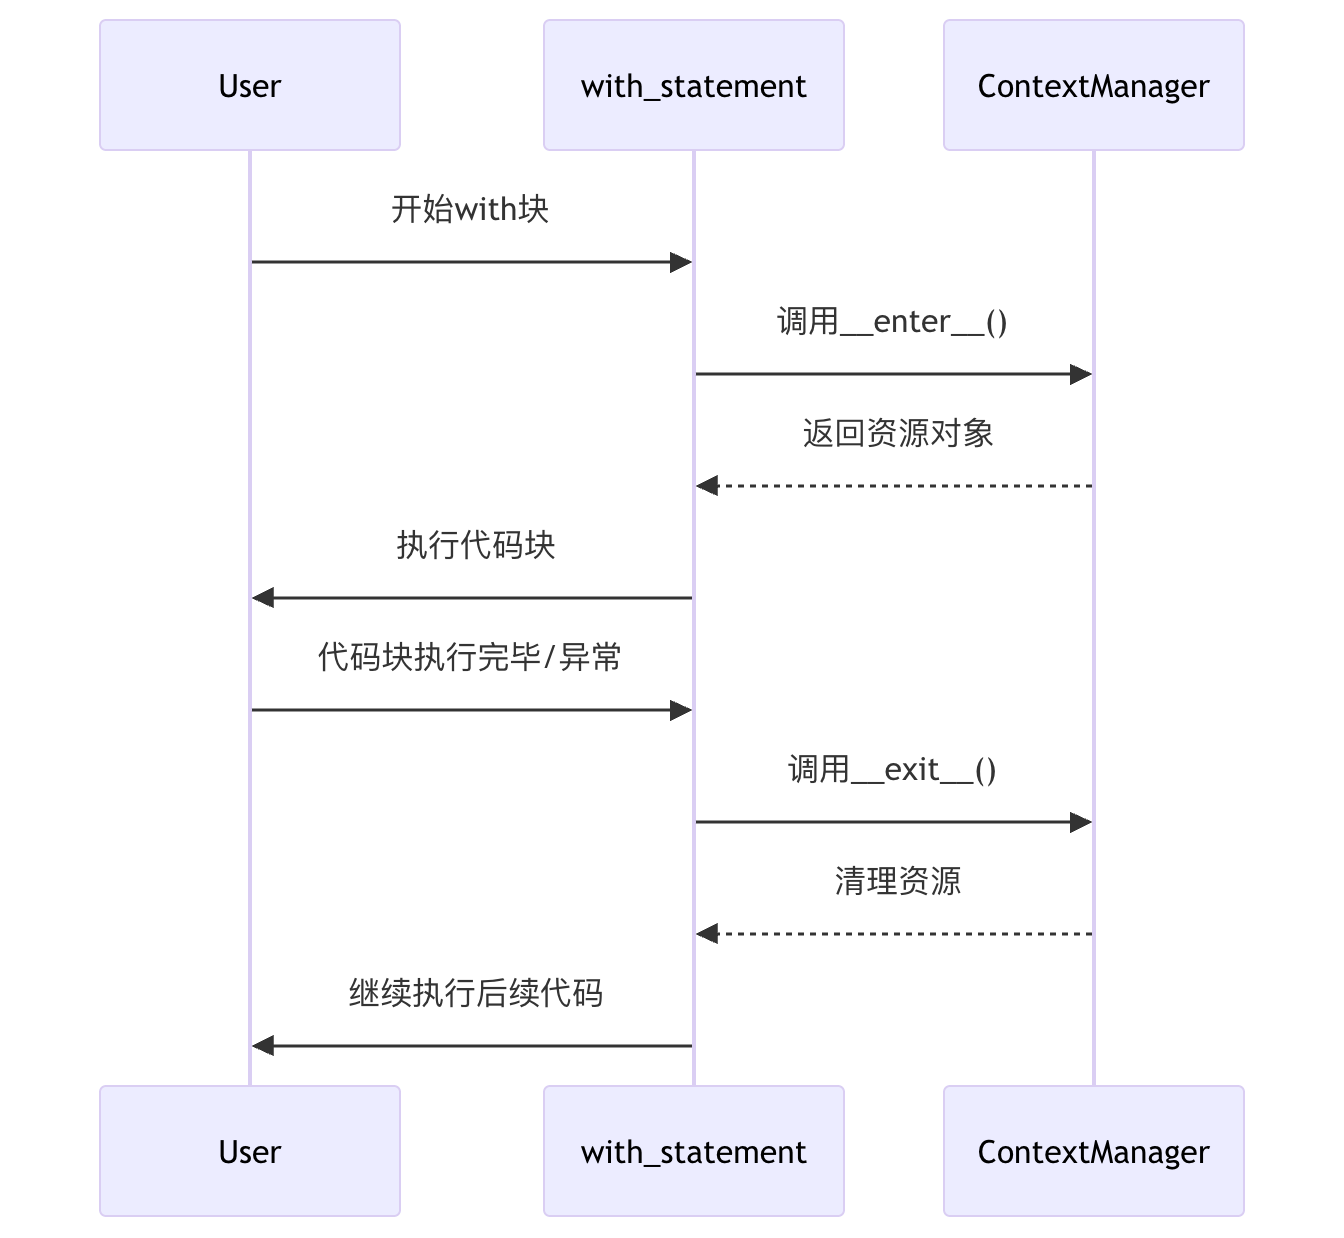
\includegraphics[width=0.6\textwidth]{part/存储/上下文管理/pic/with上下文管理执行流程.png}
    \caption{with 上下文管理执行流程}
\end{figure}


\section{创建自定义的上下文管理器}
\subsection{类的方式}
我们可以通过实现 \codeinline{\_\_enter\_\_()} 和 \codeinline{\_\_exit\_\_()} 方法创建自定义的上下文管理器
\begin{lstlisting}[style=demostyle,numbers=none]
def __enter__(self):
    # 创建资源
    return self
    
'''
exc_type：异常类型
exc_val：异常值
exc_tb：异常追踪信息

如果 __exit__() 返回 True，则表示异常已被处理，不会继续传播；返回 False 或 None，异常会继续向外传播。
'''    
def __exit__(self, exc_type, exc_val, exc_tb):
    # 释放资源
    return False    
\end{lstlisting}

\begin{lstlisting}[style=pythonstyle]
class Timer:
    def __enter__(self):
        import time
        self.start = time.time()
        return self
    
    def __exit__(self, exc_type, exc_val, exc_tb):
        import time
        self.end = time.time()
        print(f"耗时: {self.end - self.start:.2f}秒")
        return False

# 使用示例
with Timer() as t:
    # 执行一些耗时操作
    sum(range(1000000))
\end{lstlisting}

\subsection{contextlib 模块}
\begin{lstlisting}[style=pythonstyle]
from contextlib import contextmanager

@contextmanager
def tag(name):
    print(f"<{name}>")
    yield
    print(f"</{name}>")

# 使用示例
with tag("h1"):
    print("这是一个标题")
\end{lstlisting}    


%%%%%%%%%%%%%%%%%%%%%%%%%%%%%%%%%%%%%%%%%%
% 编程范式
%%%%%%%%%%%%%%%%%%%%%%%%%%%%%%%%%%%%%%%%%%
\part{[编程范式] 面向对象编程}
\chapter{面向对象}

\section{类与对象}
\subsection{类}
定义一个类，使用关键字\texttt{class}，类名的命名规则与变量名相同，首字母大写。

\begin{lstlisting}[style=demostyle,numbers=none]
class Person[(father)]: # 类首字母大写 [] 部分可选，表示继承的父类
    def __init__(self, name, age):
        self.name = name
        self.age = age

    def say(self):
        print('hello world')

p = Person('Tom', 20) # 实例化
print(p.name)
print(p.age)
p.say()
\end{lstlisting}

\subsection{继承}
Python支持多继承，使用逗号分隔。
\begin{lstlisting}[style=demostyle,numbers=none]
class Teacher:
    def teaching(self):
        print('I am teaching')

class Dad:
    def cooking(self):
        print('I am cooking')

class Son(Teacher, Dad):
    def playing(self):
        print('I am playing')

s = Son()
s.teaching()
s.cooking()
s.playing()
\end{lstlisting}

\subsection{接口}
Python中没有接口的概念，但是可以使用抽象类来实现接口的功能。
\begin{lstlisting}[style=demostyle,numbers=none]
class Animal:
    def run(self):
        pass # 占位符

class Dog(Animal):
    def run(self):
        print('dog is running')

class Cat(Animal):
    def run(self):
        print('cat is running')

d = Dog()
d.run()

c = Cat()
c.run()
\end{lstlisting}


\subsection{封装}
\subsubsection{私有属性}
Python中没有私有属性的概念，但是可以通过在属性名前加两个下划线来实现私有属性。
\begin{lstlisting}[style=demostyle,numbers=none]
class Person:
    def __init__(self, name, age):
        self.__name = name
        self.__age = age

    def say(self):
        print('hello world')

p = Person('Tom', 20)
print(p.__name) # 不能访问

p.say()
\end{lstlisting}

\subsubsection{私有方法}
Python中没有私有方法的概念，但是可以通过在方法名前加一个下划线来实现私有方法。
\begin{lstlisting}[style=demostyle,numbers=none]
class Person:
    def __init__(self, name, age):
        self.__name = name
        self.__age = age

    def __say(self):
        print('hello world')

    def say(self):
        self.__say()     

p = Person('Tom', 20)
p.say()
\end{lstlisting}

\subsection{多态}
多态是指不同的对象对同一消息做出不同的响应。
\begin{lstlisting}[style=demostyle,numbers=none]
class Animal:
    def run(self):
        pass

class Dog(Animal):
    def run(self):
        print('dog is running')

class Cat(Animal):
    def run(self):
        print('cat is running')

def run(animal):
    animal.run()

d = Dog()
run(d)

c = Cat()
run(c)
\end{lstlisting}






\part{图形可视化}
\chapter{PySide概述}

\section{PySide简介}
PySide6是Qt官方支持和维护的Python绑定库，它允许开发者在Python中创建基于Qt的图形用户界面（GUI）应用程序。与PyQt相比，PySide6在最新版本的Qt中得到了官方支持，并且使用LGPL许可证，这意味着你可以在自己的项目中使用PySide6，而不需要开源你的应用程序的源代码

简单来说，PySide6 就是将 Qt 6 提供的功能“翻译”成 Python 语言，让你可以用 Python 来开发图形界面应用程序。

\subsection{Qt 、PyQt 、PySide 之间的关系}
Qt 是一个广泛使用的框架，用于开发跨平台的图形用户界面（GUI）应用程序。它提供了创建桌面和移动应用程序的工具。

PyQt 和 PySide 是两种流行的 Python 绑定库，允许你用 Python 编写 Qt 应用程序。
\begin{enumerate}[label=\arabic*)]
    \item Qt：这是一个用 C++ 编写的核心框架，用于开发 GUI 应用程序。它包括小部件、图形、网络等库。
    \item PyQt：
    \begin{enumerate}[itemindent=1em,label=\arabic*)]
        \item 由 Riverbank Computing 开发。
        \item 提供了 Qt 库到 Python 的绑定。
        \item 通常使用 GPL 或商业许可证，这可能要求为专有软件购买许可证。
    \end{enumerate}
    
    \item PySide：
    \begin{enumerate}[itemindent=1em,label=\arabic*)]
        \item 由 Qt 公司（之前是诺基亚和 Digia）开发。
        \item 提供了 Qt 库到 Python 的绑定。
        \item 使用 LGPL 许可证，这允许更灵活的许可证，尤其适用于商业应用程序。
    \end{enumerate}
\end{enumerate}

PySide6/PyQt6都是基于Qt6, 它们之间的代码没什么区别；PySide2/PyQt5都是基于Qt5, 它们之间的代码也没什么区别。
以下代码可以相互替换
\begin{lstlisting}[style=demostyle,numbers=none]
from PySide6 import *
from PyQt6 import *
\end{lstlisting}
\begin{lstlisting}[style=demostyle,numbers=none]
from PySide2 import *
from PyQt5 import *
\end{lstlisting}

\subsection{PySide与PyQt的比较}
\begin{enumerate}[label=\arabic*)]
    \item 信号与槽的命名：

    下面代码等价：
    \begin{lstlisting}[style=demostyle,numbers=none]
    from PySide6.QtCore import Signal, Slot
    from PyQt6.QtCore import pyqtSignal as Signal, pyqtSlot as Slot
    \end{lstlisting}

    \item 枚举类型的快捷方式：
    \begin{lstlisting}[style=demostyle,numbers=none]
    Qt.Wednesday            # PySide6
    Qt.DayOfWeek.Wednesday  # PyQt6/PySide6
    \end{lstlisting}

    但是有\codeinline{qtpy}模块，使得PySide和PyQt可以通用，不需要修改代码,即使Python环境下只有 PyQt6 和 qtpy 模块，也可以运行 PySide6 的代码。
    \begin{lstlisting}[style=demostyle,numbers=none]
    from qtpy.QtCore import Qt
    \end{lstlisting}
\end{enumerate}



\subsection{主要模块}
\begin{enumerate}[label=\arabic*)]
    \item QtCore：
    提供核心功能，如事件处理、定时器、文件和目录操作、线程等。
    \item QtGui：
    提供图形功能，如 2D 图形绘制、字体、图像和窗口管理。
    \item QtWidgets：
    提供传统的桌面小部件，用于构建经典的用户界面组件。
    \item QtQuick 和 QML：
    支持现代的声明式用户界面设计，适用于创建动态和交互丰富的界面。
    \item QtNetwork：
    提供网络功能，如 TCP/IP 套接字、HTTP 请求等。
    \item QtSql：
    提供对 SQL 数据库的访问和操作功能。
\end{enumerate}


\section{安装PySide}
\url{https://doc.qt.io/qtforpython-6/quickstart.html#}
\begin{lstlisting}[style=demostyle,numbers=none]
$> conda create --name myenv python=3.9
$> conda activate myPySide
$> pip install pyside6
$> pip install pyside6==6.4.1

# 查看已安装的包
$> pip list | grep PySide6
$> pip show pyside6
Name: PySide6
Version: 6.7.2
Summary: Python bindings for the Qt cross-platform application and UI framework
Home-page: https://pyside.org
Author:
Author-email: Qt for Python Team <pyside@qt-project.org>
License: LGPL
Location: /home/tony/.application/Miniconda/envs/myPySide/lib/python3.9/site-packages
Requires: PySide6-Addons, PySide6-Essentials, shiboken6
Required-by:
\end{lstlisting}

\subsection{常见问题}

\begin{figure}[htpb]
    \centering
    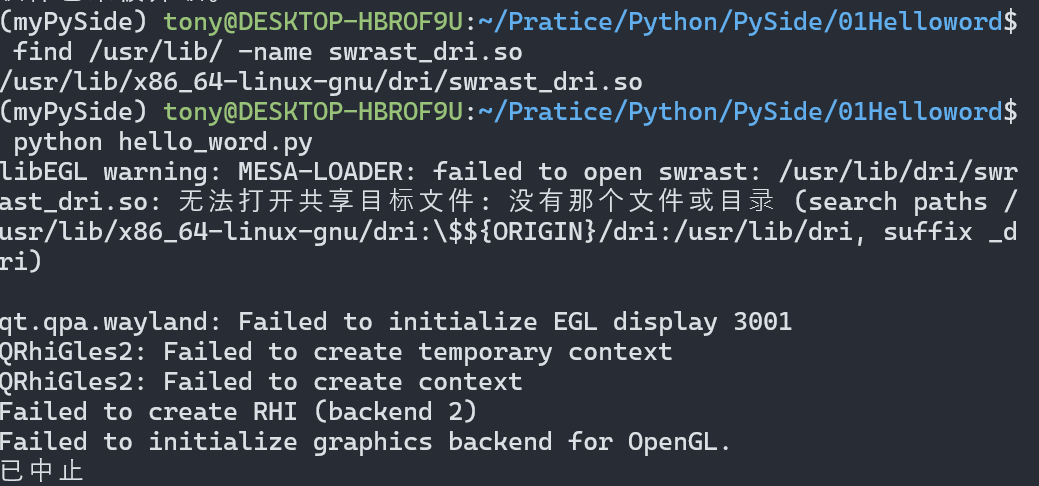
\includegraphics[width=0.6\textwidth]{part/图形化/pic/PySide/找不到swrast.png}
    \caption{找不到swrast}
    \label{fig:NotFoundSwrast}
\end{figure}

    
\subsubsection{PySide找不到libstdc++}
\begin{figure}[htpb]
    \centering
    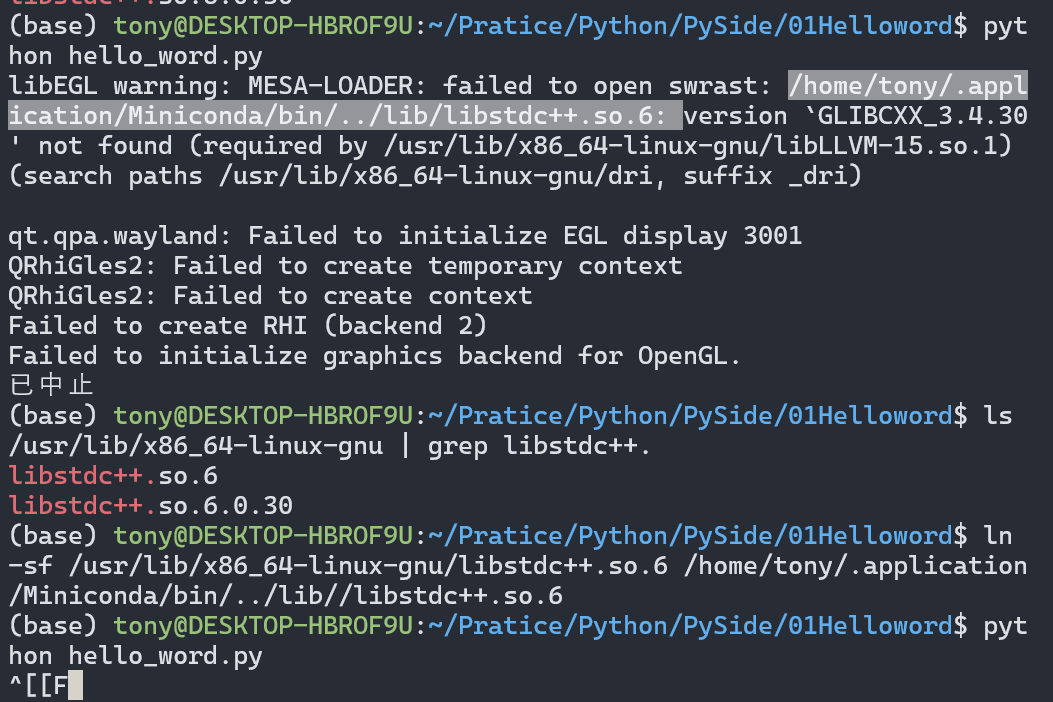
\includegraphics[width=0.6\textwidth]{part/图形化/pic/PySide/PySide找不到libstdc++.png}
    \caption{PySide找不到libstdc++}
    \label{fig:PySideNotFoundLibstdc++}
\end{figure}

\begin{lstlisting}[style=demostyle,numbers=none]
ln -sf /usr/lib/x86_64-linux-gnu/libstdc++.so.6 /home/tony/.application/Miniconda/bin/../lib/libstdc++.so.6
\end{lstlisting}

\subsubsection{conda的python版本与系统的版本不一致}

\begin{figure}[htpb]
    \centering
    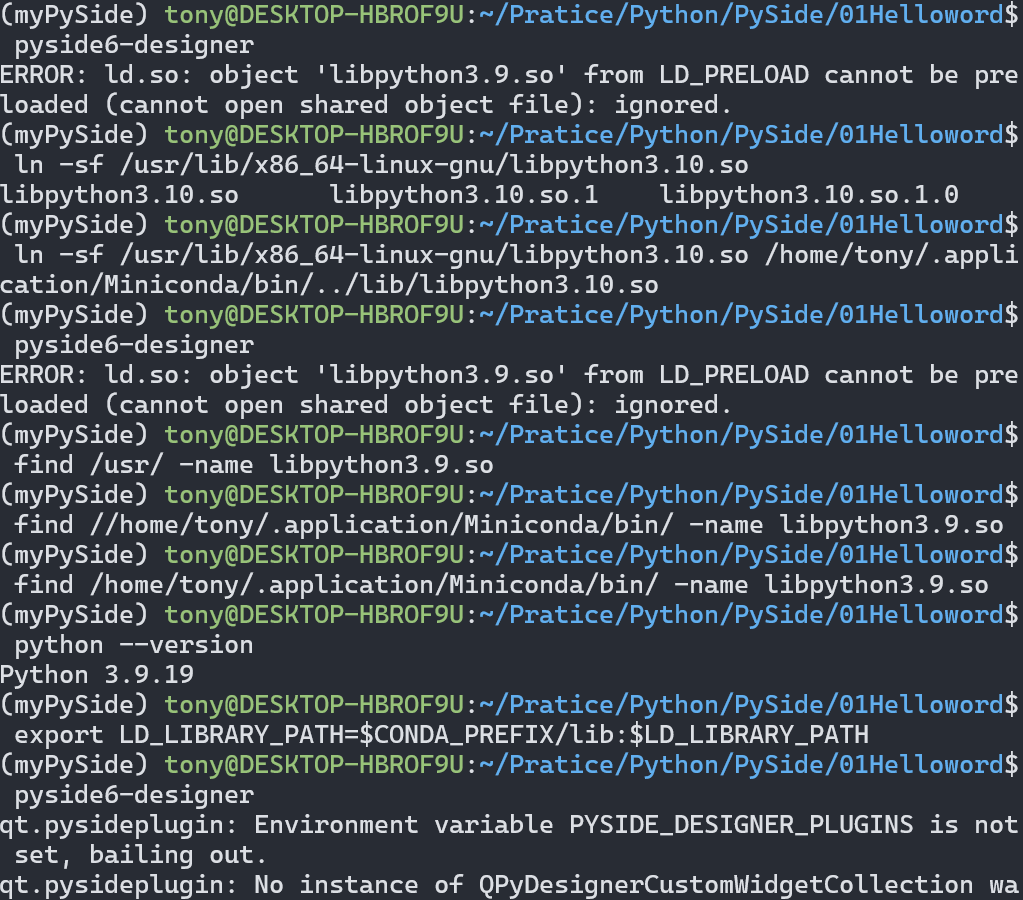
\includegraphics[width=0.6\textwidth]{part/图形化/pic/PySide/conda的python版本与系统的版本不一致.png}
    \caption{conda的python版本与系统的版本不一致}
    \label{fig:CondaPythonVersionNotMatch}
\end{figure}

\begin{lstlisting}[style=demostyle,numbers=none]
export LD_LIBRARY_PATH=$CONDA_PREFIX/lib:$LD_LIBRARY_PATH
\end{lstlisting}


%% Matplotlib
\chapter{[Python库] Matplotlib概述}

\section{简介}
matplotlib 是 python 中一个非常强大的 2D 函数绘图模块，
它提供了子模块 \codeinline{pyplot} 和 \codeinline{pylab}。

pylab 是对 pyplot 和 numpy 模块的封装，更适合在 IPython 交互式环境中使用。

对于一个项目来说，官方建议分别导入使用，这样代码更清晰，即：
\begin{lstlisting}[style=pythonstyle]
import numpy as np
import matplotlib.pyplot as plt

# 不要使用
import pylab as pl
\end{lstlisting}

\section{安装}
\begin{lstlisting}[style=demostyle,numbers=none]
conda install matplotlib
# 或
pip install matplotlib
\end{lstlisting}



\section{基本框架}
\begin{lstlisting}[style=pythonstyle]
# 分别导入 numpy 和 pyplot 模块
import numpy as np
import matplotlib.pyplot as plt

# 生成 X 坐标，256个采样值足够图像平滑
X = np.linspace(-np.pi, np.pi, 256, endpoint=True)

# 生成 Y 坐标
C,S = np.cos(X), np.sin(X)

# 绘制正余弦
plt.plot(X,S)
plt.plot(X,C)

# 显示图像
plt.show()
\end{lstlisting}

\begin{lstlisting}[style=demostyle,numbers=none]
# 必须导入的库
import matplotlib.pyplot as plt
# legend 功能：用于为图形添加图例
plt.legend(*args, **kwargs)
# 参数说明：
# loc : 图例的位置
## 'best'：自动选择最佳位置
## 'upper right'：右上角
## 'upper left'：左上角
## 'lower left'：左下角
## 'lower right'：右下角
## 'right'：右侧
## 'center left'：左侧居中
## 'center right'：右侧居中
## 'lower center'：底部居中
## 'upper center'：顶部居中
## 'center'：中央
# fontsize : 图例文字的大小
# title : 图例标题
# shadow : 是否添加阴影
# bbox_to_anchor : 图例相对于图形的位置
\end{lstlisting}

\begin{lstlisting}[style=demostyle,numbers=none]
# 必须导入的库
import matplotlib.pyplot as plt
# title 功能：为图表添加标题
plt.title(label, fontdict=None, loc='center', pad=None, **kwargs)
# 参数说明：
# label : 标题文本
# fontdict : 设置字体的字典，如字体大小、颜色等
# loc : 标题的位置
## 'left'：左对齐
## 'center'：居中对齐
## 'right'：右对齐
# pad : 标题与图像之间的间距
\end{lstlisting}

\begin{lstlisting}[style=demostyle,numbers=none]
# 必须导入的库
import matplotlib.pyplot as plt
# show 功能：显示当前所有绘图
plt.show(*args, **kwargs)
# 参数说明：
# block : 是否阻塞脚本的运行，直到窗口关闭
## True：阻塞（默认）
## False：不阻塞
\end{lstlisting}
\chapter{[matplotlib] 绘图}
\section{折线/散点图}
\subsection{plt.plot 折线/散点图}
\codeinline{plt.plot()} 用于绘制散点图，默认情况下，\codeinline{plt.plot(x, y)} 会连接每个点，生成一条平滑的连线图。

\begin{lstlisting}[style=demostyle,numbers=none]
# 必须导入的库
import matplotlib.pyplot as plt
# plot 功能：用于绘制散点图
plt.plot(*args, scalex=True, scaley=True, data=None, **kwargs)
# 参数说明：
# x : x坐标
# y : y坐标
# fmt : 线条样式
## 'o'：点
## '-o'：点连线
## '-H'：六边形连线
# data : 数据源
# scalex, scaley : 是否自动缩放x或y轴
\end{lstlisting}

\begin{lstlisting}[style=pythonstyle]
import numpy as np
import matplotlib.pyplot as plt

# 生成从 0 到 1.1，步长为 0.01 的数据
data = np.arange(0, 1.1, 0.01)

# 设置图表的标题
plt.title('lines')  # 添加标题

# 设置 x 轴和 y 轴的名称
plt.xlabel('x')  # 添加 x 轴的名称
plt.ylabel('y')  # 添加 y 轴的名称

# 设置 x 轴和 y 轴的范围
plt.xlim((0, 1))  # 确定 x 轴范围
plt.ylim((0, 1))  # 确定 y 轴范围

# 设置 x 轴和 y 轴的刻度
plt.xticks([0, 0.2, 0.4, 0.6, 0.8, 1])  # 规定 x 轴刻度
plt.yticks([0, 0.2, 0.4, 0.6, 0.8, 1])  # 确定 y 轴刻度

# 使用 plot 函数绘制连线图
plt.plot(data, data)  # 绘制 y = x 曲线
plt.plot(data, data**2)  # 绘制 y = x^2 曲线

# 添加图例
plt.legend(['y=x', r'$y=x^2$'])  # r'' 使得数学公式正确显示

# 保存图像
plt.savefig('../tmp/默认连线图.png')

# 显示图像
plt.show()
\end{lstlisting}
\begin{figure}[htpb]
    \centering
    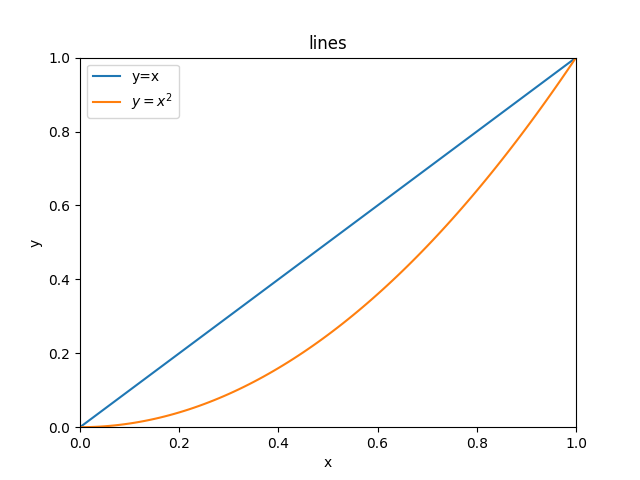
\includegraphics[width=0.4\textwidth]{part/图形化/Matplotlib/pic/绘图/plot默认连线图.png}
    \caption{plot默认连线图}
\end{figure}


\begin{lstlisting}[style=pythonstyle]
import matplotlib.pyplot as plt
import numpy as np
fig = plt.figure(figsize=(6,4))
x = np.linspace(0, 10, 30)
y = np.sin(x)

# 等价于 plt.plot(x, y, mark='o', color='blue')
plt.plot(x, y, 'ob')
\end{lstlisting}
\begin{figure}[htpb]
    \centering
    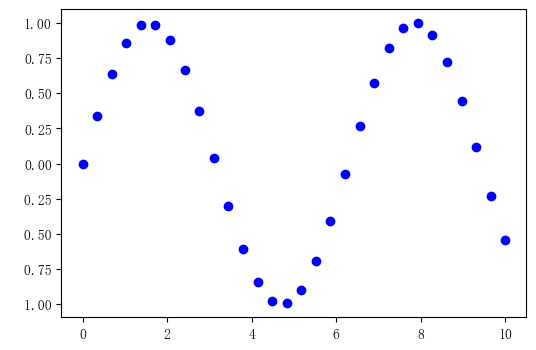
\includegraphics[width=0.6\textwidth]{part/图形化/Matplotlib/pic/绘图/plot散点图.png}
    \caption{plot散点图}
\end{figure}

\begin{lstlisting}[style=demostyle,numbers=none]
$> cat people.csv    
指标,年末总人口(万人),0-14岁人口(万人),15-64岁人口(万人),65岁及以上人口(万人)
2000年,126743,29012,88910,8821
2001年,127627,28716,89849,9062
2002年,128453,28774,90302,9377
2003年,129227,28559,90976,9692
2004年,129988,27947,92184,9857
2005年,130756,26504,94197,10055
2006年,131448,25961,95068,10419
2007年,132129,25660,95833,10636
2008年,132802,25166,96680,10956
2009年,133450,24659,97484,11307
2010年,134091,22259,99938,11894
2011年,134735,22164,100283,12288
2012年,135404,22287,100403,12714
2013年,136072,22329,100582,13161
2014年,136782,22558,100469,13755
2015年,137462,22715,100361,14386
2016年,138271,23008,100260,15003
2017年,139008,23348,99829,15831
2018年,139538,23523,99357,16658
2019年,140005,23493,98914,17599
\end{lstlisting}
\begin{lstlisting}[style=pythonstyle]
import numpy as np
import pandas as pd
import matplotlib.pyplot as plt
plt.rcParams['font.sans-serif'] =' SimHei'
# 设置中文显示
plt.rcParams['axes.unicode_minus'] = False
data = pd.read_csv('../data/people.csv')
name = data.columns  # 提取其中的columns字段，视为数据的标签
values = data.values  # 提取其中的values字段，数据的存在位置
plt.figure(figsize=(9, 7))  # 设置画布
plt.scatter(values[:, 0], values[:, 1], marker='o')  # 绘制散点图
plt.xlabel('年份')  # 添加横轴标签
plt.ylabel('年末总人口（万人）')  # 添加y轴名称
plt.xticks(range(0, 20), values[range(0, 20), 0], rotation=45)
plt.title('2000-2019年年末总人口散点图')  # 添加图表标题
plt.savefig('../tmp/2000-2019年年末总人口散点图.png') # 保存图表
plt.show()
\end{lstlisting}
\begin{figure}[htpb]
    \centering
    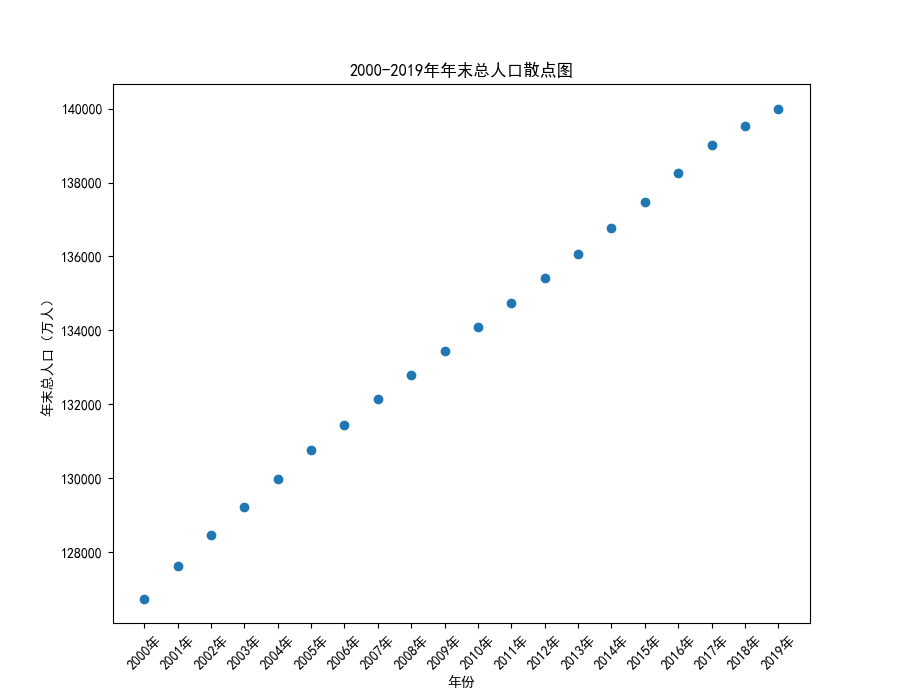
\includegraphics[width=0.6\textwidth]{part/图形化/Matplotlib/pic/绘图/2000-2019年年末总人口散点图.png}
    \caption{2000-2019年年末总人口散点图}
\end{figure}


\subsubsection{-o 将散点图连线}
使用 \codeinline{plt.plot()} 可以绘制连线的散点图。
\begin{lstlisting}[style=pythonstyle]
import matplotlib.pyplot as plt
import numpy as np

# 数据
x = np.linspace(0, 10, 30)
y = np.sin(x)

# 绘制连线的散点图
plt.plot(x, y, '-o', color='blue')  # 使用线条连接散点
plt.title('连线的散点图')
plt.show()
\end{lstlisting}

\begin{figure}[htpb]
    \centering
    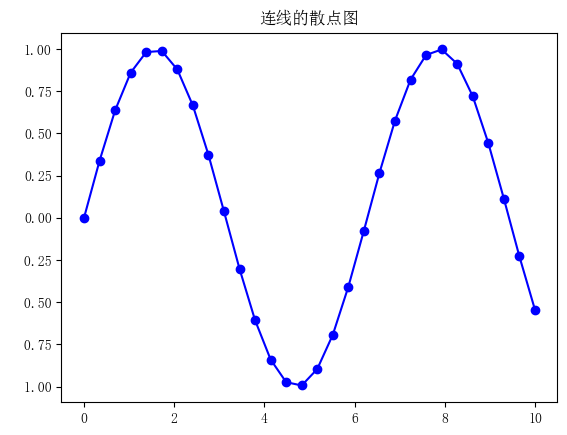
\includegraphics[width=0.6\textwidth]{part/图形化/Matplotlib/pic/绘图/连线的散点图.png}
    \caption{连线的散点图}
\end{figure}

\begin{lstlisting}[style=pythonstyle]
import numpy as np
import pandas as pd
import matplotlib.pyplot as plt

# 设置中文显示
plt.rcParams['font.sans-serif'] = 'SimHei'  # 解决中文乱码问题
plt.rcParams['axes.unicode_minus'] = False  # 设置正常显示负号

# 读取数据
data = pd.read_csv('../data/people.csv')
name = data.columns  # 提取columns字段，视为数据的标签
values = data.values  # 提取values字段，数据的存在位置

# 创建画布，并设置左右两个子图
plt.figure(figsize=(16, 7))  # 设置画布大小

# 左侧子图
plt.subplot(1, 2, 1)  # 创建第一个子图
plt.plot(values[:, 0], values[:, 1], color='r', linestyle='--', marker='o')  # 绘制折线图
plt.xlabel('年份')  # 添加横轴标签
plt.ylabel('年末总人口（万人）')  # 添加y轴名称
plt.xticks(range(0, 20), values[range(0, 20), 0], rotation=45)
plt.title('2000-2019年年末总人口点线图')  # 添加图表标题

# 右侧子图
plt.subplot(1, 2, 2)  # 创建第二个子图
plt.plot(values[:, 0], values[:, 2], 'bs-',  # 蓝色方块实线
         values[:, 0], values[:, 3], 'ro-.',  # 红色圆点虚线
         values[:, 0], values[:, 4], 'gH--')  # 绿色六边形点划线
plt.xlabel('年份')  # 添加横轴标签
plt.ylabel('年末总人口（万人）')  # 添加y轴名称
plt.xticks(range(0, 20), values[range(0, 20), 0], rotation=45)
plt.title('2000-2019年各年龄段总人口点线图')  # 添加图表标题
plt.legend(['0-14岁人口', '15-64岁人口', '65岁及以上人口'])

# 保存合并的图表
plt.tight_layout()  # 调整子图布局，避免重叠
plt.savefig('../tmp/2000-2019年总人口点线图.png')
plt.show()
\end{lstlisting}
\begin{figure}[htpb]
    \centering
    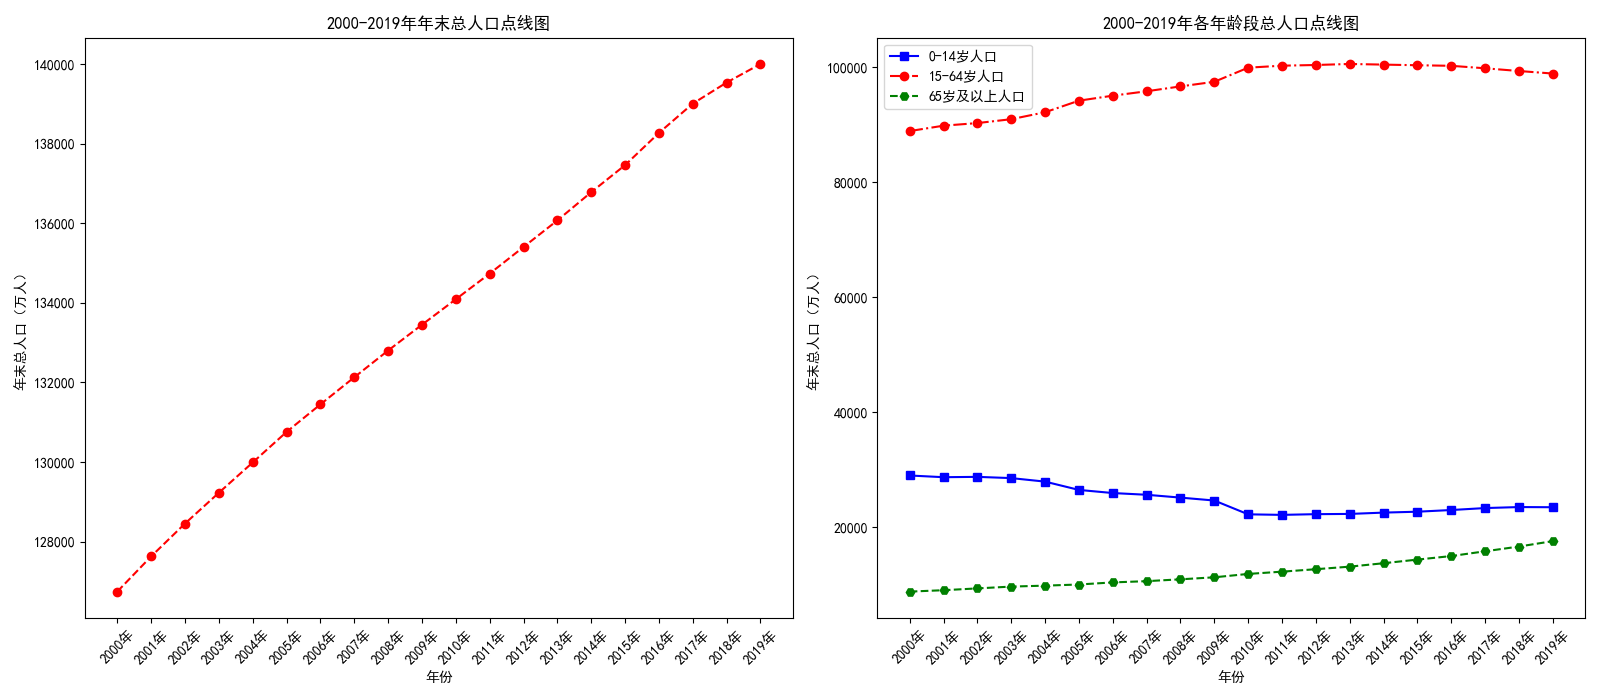
\includegraphics[width=0.6\textwidth]{part/图形化/Matplotlib/pic/绘图/2000-2019年总人口点线图.png}
    \caption{2000-2019年总人口点线图}
\end{figure}



\subsubsection{设置散点图属性}
\begin{lstlisting}[style=pythonstyle]
import matplotlib.pyplot as plt
import numpy as np
fig = plt.figure(figsize=(6,4))
x = np.linspace(0, 10, 30)
y = np.sin(x)

plt.plot(x, y, '-H', color='gray',   # 线条颜色 -H 代表六边形
         markersize=15, linewidth=4, # 标记大小，线宽
         markerfacecolor='white',    # 标记填充色
         markeredgecolor='gray',     # 标记边框色
         markeredgewidth=2)          # 标记边框宽度
\end{lstlisting}

\begin{figure}[htpb]
    \centering
    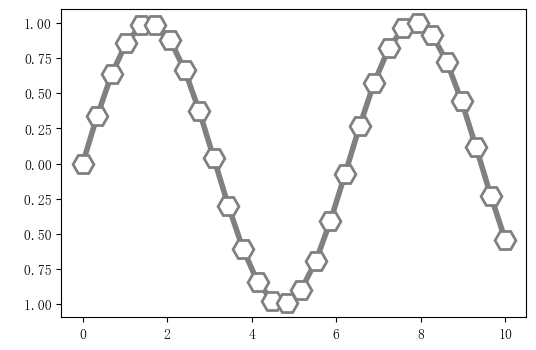
\includegraphics[width=0.6\textwidth]{part/图形化/Matplotlib/pic/绘图/设置散点图属性.png}
    \caption{设置散点图属性}
\end{figure}

\subsubsection{绘制折线图}
\begin{lstlisting}[style=pythonstyle]
import numpy as np
import pandas as pd
import matplotlib.pyplot as plt
plt.rcParams['font.sans-serif'] =' SimHei'
# 设置中文显示
plt.rcParams['axes.unicode_minus'] = False
data = pd.read_csv('../data/people.csv')
name = data.columns  # 提取其中的columns字段，视为数据的标签
values = data.values  # 提取其中的values字段，数据的存在位置    
plt.figure(figsize=(9, 7))  # 设置画布
plt.plot(values[:, 0], values[:, 1], color='r', linestyle='--')  # 绘制折线图
plt.xlabel('年份')  #添加横轴标签
plt.ylabel('年末总人口（万人）')  # 添加y轴名称
plt.xticks(range(0, 20), values[range(0, 20), 0], rotation=45)
plt.title('2000-2019年年末总人口折线图')  # 添加图表标题
plt.savefig('../tmp/2000-2019年年末总人口折线图.png')
plt.show()
\end{lstlisting}
\begin{figure}[htpb]
    \centering
    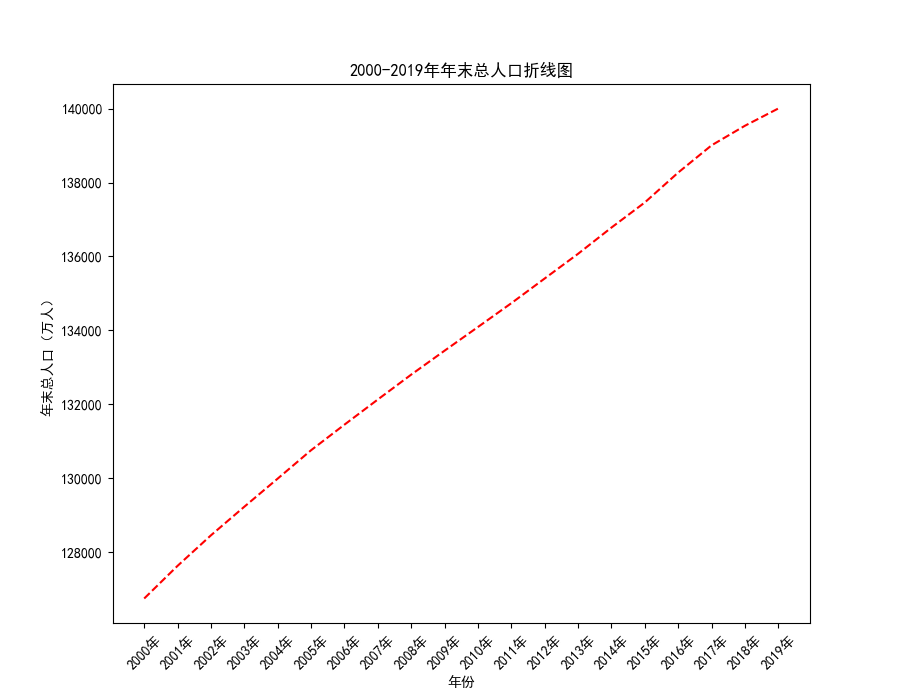
\includegraphics[width=0.6\textwidth]{part/图形化/Matplotlib/pic/绘图/2000-2019年年末总人口折线图.png}
    \caption{2000-2019年年末总人口折线图}
\end{figure}


\subsection{plt.scatter 散点图}
\codeinline{plt.scatter()} 用于绘制散点图，允许设置点的大小、颜色、形状等属性。
\begin{lstlisting}[style=demostyle,numbers=none]
scatter(x, y, s=None, c=None, marker=None, cmap=None, norm=None, vmin=None, vmax=None,
        alpha=None, linewidths=None, verts=None, edgecolors=None,
        hold=None, data=None, **kwargs)
# 参数说明：
# x : x坐标
# y : y坐标
# s : 点的大小
# c : 点的颜色
# marker : 点的形状
# cmap : 颜色映射表
# alpha : 透明度
# edgecolors : 点的边缘颜色
\end{lstlisting}

\begin{lstlisting}[style=pythonstyle]
import matplotlib.pyplot as plt
import numpy as np

# 数据
x = np.random.rand(50)
y = np.random.rand(50)
sizes = np.random.rand(50) * 1000  # 点的大小
colors = np.random.rand(50)        # 点的颜色

# 绘制散点图
plt.scatter(x, y, s=sizes, c=colors, alpha=0.6, cmap='viridis')
plt.colorbar()  # 添加颜色条
plt.title('散点图示例')
plt.show()
\end{lstlisting}

\begin{lstlisting}[style=pythonstyle]
import numpy as np
import pandas as pd
import matplotlib.pyplot as plt
plt.rcParams['font.sans-serif'] =' SimHei'
# 设置中文显示
plt.rcParams['axes.unicode_minus'] = False
data = pd.read_csv('../data/people.csv')
name = data.columns  # 提取其中的columns字段，视为数据的标签
values = data.values  # 提取其中的values字段，数据的存在位置    
plt.figure(figsize=(9, 7))  # 设置画布
plt.scatter(values[:, 0], values[:, 2], marker='o', c='red')   # 选取values中的第一列和第三列数据绘制散点图
plt.scatter(values[:, 0], values[:, 3], marker='D', c='blue')  # 选取values中的第一列和第四列数据绘制散点图
plt.scatter(values[:, 0], values[:, 4], marker='v', c='black') # 选取values中的第一列和第五列数据绘制散点图
plt.xlabel('年份')  # 添加横轴标签
plt.ylabel('年末总人口（万人）')  # 添加纵轴标签
plt.xticks(range(0, 20), values[range(0, 20), 0], rotation=45)
plt.title('2000-2019年各年龄段年末总人口散点图')  # 添加图表标题
plt.legend(['0-14岁人口', '15-64岁人口', '65岁及以上人口'])  #添加图例
plt.savefig('../tmp/2000-2019年各年龄段年末总人口散点图.png')
plt.show()
\end{lstlisting}
\begin{figure}[htpb]
    \centering
    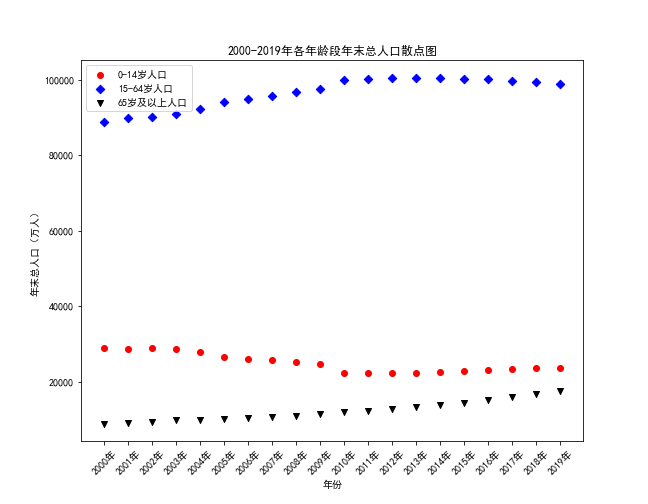
\includegraphics[width=0.5\textwidth]{part/图形化/Matplotlib/pic/绘图/2000-2019年各年龄段年末总人口数散点图.png}
    \caption{2000-2019年各年龄段年末总人口数散点图}
\end{figure}


\begin{lstlisting}[style=pythonstyle]
import matplotlib.pyplot as plt
import numpy as np

def scatter_create_color_graph():
    """
    绘制不同颜色值的散点图。
    x, y: 散点的坐标
    c: 颜色值（以十六进制表示）
    """
    x = [i for i in range(20)]
    y = [i for i in range(20)]

    plt.xticks(x)
    plt.yticks(y)
    c = np.linspace(0, 0xffffff, 20, endpoint=False)
    plt.scatter(x, y, c=c, s=200, marker='o')
    plt.title('不同颜色值绘制的散点图')

def scatter_create_markers_graph():
    """
    绘制不同标记大小和颜色的散点图。
    marker: 标记类型
    s: 标记大小
    c: 标记颜色
    """
    x = np.array([i for i in range(20)])
    y = np.array([i for i in range(20)])

    plt.xticks(x)
    plt.yticks(y)
    plt.scatter(x, y, c='orange', s=200, marker='v')
    plt.scatter(x + 1, y, c='gray', s=100, marker='^')
    plt.title('不同标记大小和颜色绘制的散点图')

def scatter_create_size_graph():
    """
    根据坐标调整标记大小的散点图。
    s: 根据位置动态调整标记大小
    """
    x = np.array([i for i in range(10)])
    y = np.array([0] * len(x))
    plt.ylim(-0.5, 1.5)
    plt.yticks([0, 1])
    plt.xticks(x)

    sizes = [20 * (n + 1) ** 2 for n in range(len(x))]
    plt.scatter(x, y, c='m', s=sizes)

    sizes = [20 * (10 - n) ** 2 for n in range(len(x))]
    plt.scatter(x, y + 1, c='m', s=sizes)
    plt.title('根据坐标调整标记大小')

def scatter_create_random_graph():
    """
    随机坐标散点图。
    x, y: 随机生成的坐标
    marker: 标记类型
    s: 标记大小
    alpha: 标记透明度
    """
    x = np.random.randn(100)
    y = np.random.randn(100)

    plt.scatter(x, y, c='m', marker='p', s=500, alpha=0.6)
    plt.title('随机坐标散点图')

def scatter_create_guess_graph():
    """
    多元高斯分布二维图。
    s: 根据分布值调整标记大小
    alpha: 标记透明度
    """
    mu_vec = np.array([0,0])
    cov_mat = np.array([[1,0],[0,1]])
    X = np.random.multivariate_normal(mu_vec, cov_mat, 1000)
    R = X ** 2
    R_sum = R.sum(axis = 1)

    plt.scatter(X[:,0], X[:,1], color='m', marker='o',
                s = 32.*R_sum, edgecolor='black', alpha=0.5)
    plt.title('多元高斯分布二维图')

def scatter_create_gradual_graph():
    """
    绘制同点渐变晕化效果。
    c: 渐变颜色值
    s: 标记大小
    """
    c = np.linspace(0xffff00, 0xffffff, 20, endpoint=False)
    for i in range(19,-1,-1):
        size = i * 10000 + 10
        cval = hex(int(c[i]))[2:]
        color = "#" + '0' * (6 - len(cval)) + cval
        plt.scatter(0, 0, s=size, c=color)
    plt.title('同点渐变晕化')

# 创建3x2的子图布局
plt.figure(figsize=(15, 10))

# 绘制每个子图
plt.subplot(3, 2, 1)
scatter_create_color_graph()

plt.subplot(3, 2, 2)
scatter_create_markers_graph()

plt.subplot(3, 2, 3)
scatter_create_size_graph()

plt.subplot(3, 2, 4)
scatter_create_random_graph()

plt.subplot(3, 2, 5)
scatter_create_guess_graph()

plt.subplot(3, 2, 6)
scatter_create_gradual_graph()

# 调整布局并显示图像
plt.tight_layout()
plt.show()   
\end{lstlisting}

\begin{figure}[htpb]
    \centering
    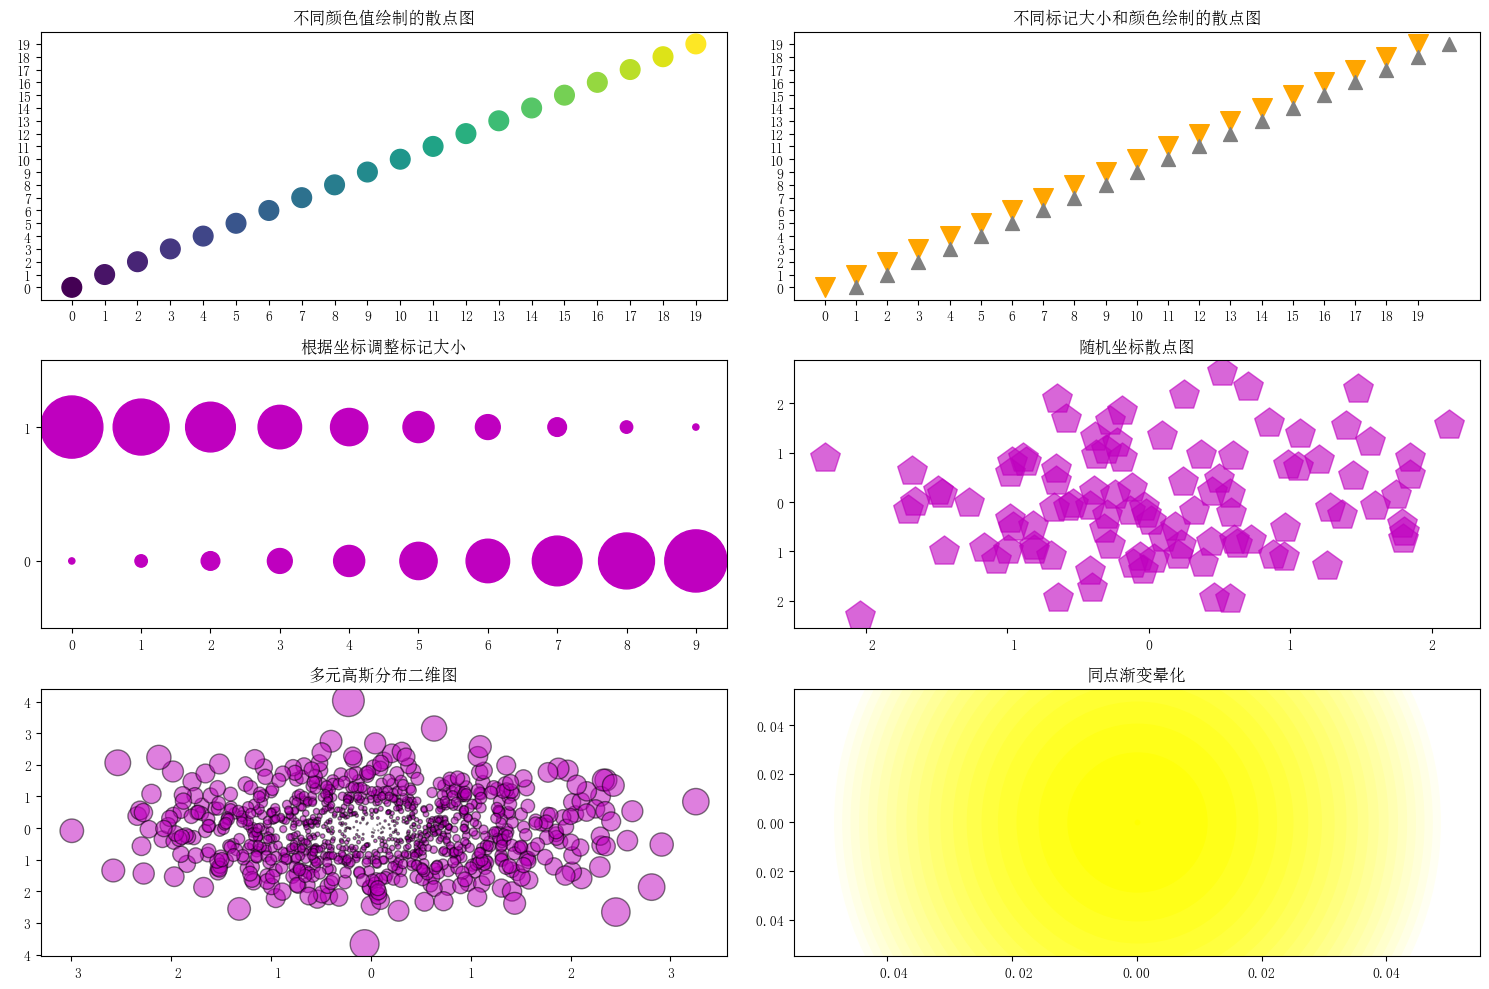
\includegraphics[width=0.6\textwidth]{part/图形化/Matplotlib/pic/绘图/不同scatter属性演示.png}
    \caption{不同scatter属性演示}
\end{figure}

\section{条形图/柱形图}
\subsection{plt.bar 垂直条形图}
\codeinline{plt.bar()} 用于绘制垂直的条形图。
\begin{lstlisting}[style=demostyle,numbers=none]
# 必须导入的库
import matplotlib.pyplot as plt
# bar 功能：绘制垂直条形图
plt.bar(x, height, width=0.8, bottom=None, align='center', **kwargs)
# 参数说明：
# x : 条形的 x 坐标
# height : 条形的高度
# width : 条形的宽度
# bottom : 条形的底部位置
# align : 对齐方式
## 'center'：居中
## 'edge'：边缘对齐
\end{lstlisting}

\begin{lstlisting}[style=pythonstyle]
import matplotlib.pyplot as plt

# 数据
categories = ['A', 'B', 'C', 'D']
values = [10, 24, 36, 12]

# 绘制垂直条形图
plt.bar(categories, values, color='skyblue')
plt.title('垂直条形图')
plt.show()
\end{lstlisting}
\begin{figure}[htpb]
    \centering
    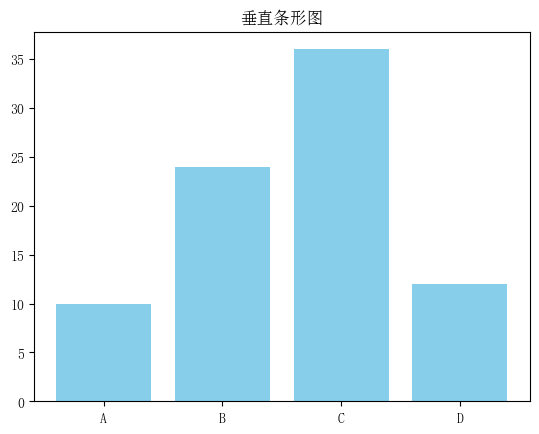
\includegraphics[width=0.6\textwidth]{part/图形化/Matplotlib/pic/绘图/垂直条形图.png}
    \caption{垂直条形图}
\end{figure}


\subsection{plt.bar 堆叠条形图}
\codeinline{plt.bar()} 可以通过设置底部来实现堆叠条形图。
\begin{lstlisting}[style=pythonstyle]
import matplotlib.pyplot as plt

# 数据
categories = ['A', 'B', 'C', 'D']
values1 = [10, 20, 30, 40]
values2 = [5, 15, 25, 10]

# 绘制堆叠条形图
plt.bar(categories, values1, color='lightblue', label='Values 1')
plt.bar(categories, values2, bottom=values1, color='orange', label='Values 2')
plt.title('堆叠条形图')
plt.legend()
plt.show()
\end{lstlisting}

\begin{figure}[htpb]
    \centering
    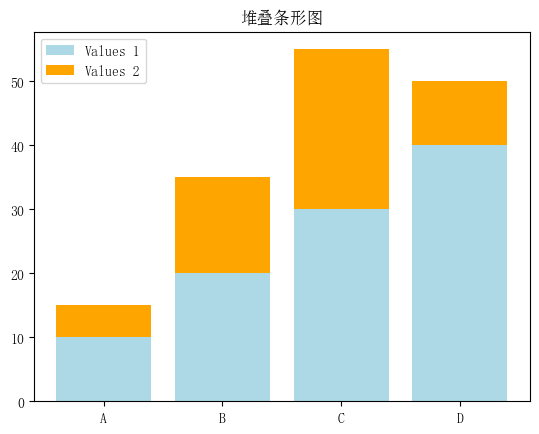
\includegraphics[width=0.6\textwidth]{part/图形化/Matplotlib/pic/绘图/堆叠条形图.png}
    \caption{堆叠条形图}
\end{figure}


\subsection{plt.bar 并列条形图}
并列条形图可以通过调整条形的宽度和位置来实现。
\begin{lstlisting}[style=pythonstyle]
import matplotlib.pyplot as plt
import numpy as np

# 数据
categories = np.arange(4)
values1 = [10, 20, 30, 40]
values2 = [5, 15, 25, 10]

# 绘制并列条形图
plt.bar(categories - 0.2, values1, width=0.4, color='lightblue', label='Values 1')
plt.bar(categories + 0.2, values2, width=0.4, color='orange', label='Values 2')
plt.title('并列条形图')
plt.legend()
plt.show()
\end{lstlisting}
\begin{figure}[htpb]
    \centering
    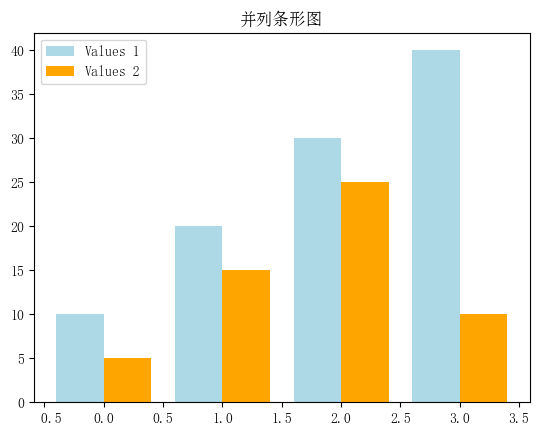
\includegraphics[width=0.6\textwidth]{part/图形化/Matplotlib/pic/绘图/并列条形图.png}
    \caption{并列条形图}
\end{figure}


\subsection{plt.barh 水平条形图}
\codeinline{plt.barh()} 用于绘制水平条形图。
\begin{lstlisting}[style=demostyle,numbers=none]
# 必须导入的库
import matplotlib.pyplot as plt
# barh 功能：绘制水平条形图
plt.barh(y, width, height=0.8, left=None, align='center', **kwargs)
# 参数说明：
# y : 条形的 y 坐标
# width : 条形的宽度
# height : 条形的高度
# left : 条形的左侧位置
# align : 对齐方式
## 'center'：居中
## 'edge'：边缘对齐
\end{lstlisting}
\begin{lstlisting}[style=pythonstyle]
import matplotlib.pyplot as plt

# 数据
categories = ['A', 'B', 'C', 'D']
values = [10, 24, 36, 12]

# 绘制水平条形图
plt.barh(categories, values, color='skyblue')
plt.title('水平条形图')
plt.show()
\end{lstlisting}
\begin{figure}[htpb]
    \centering
    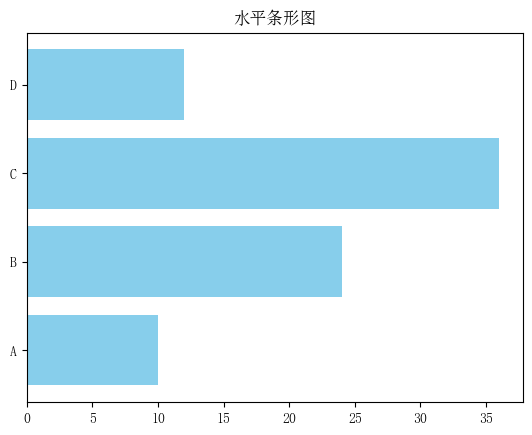
\includegraphics[width=0.6\textwidth]{part/图形化/Matplotlib/pic/绘图/水平条形图.png}
    \caption{水平条形图}
\end{figure}


% \section{折线图}
% \label{sec:matplotlib_line}
% \codeinline{plt.plot()} 用于绘制折线图。
% \begin{lstlisting}[style=pythonstyle]
% import matplotlib.pyplot as plt
% import numpy as np

% # 数据
% x = np.linspace(0, 10, 100)
% y = np.sin(x)

% # 绘制折线图
% plt.plot(x, y, color='green', linewidth=2, linestyle='--')
% plt.title('折线图')
% plt.show()
% \end{lstlisting}

\section{pie 饼图}
\codeinline{plt.pie()} 用于绘制饼图。
\begin{lstlisting}[style=demostyle,numbers=none]
# 必须导入的库
import matplotlib.pyplot as plt
# pie 功能：绘制饼图
plt.pie(x, explode=None, labels=None, colors=None, autopct=None, pctdistance=0.6, **kwargs)
# 参数说明：
# x : 每个饼块的大小
# explode : 是否突出显示饼块
# labels : 饼块的标签
# colors : 饼块的颜色
# autopct : 显示百分比的格式
# pctdistance : 标签距离圆心的比例
\end{lstlisting}
\begin{lstlisting}[style=pythonstyle]
import matplotlib.pyplot as plt

# 数据
sizes = [15, 30, 45, 10]
labels = ['A', 'B', 'C', 'D']
colors = ['gold', 'yellowgreen', 'lightcoral', 'lightskyblue']

# 绘制饼图
plt.pie(sizes, labels=labels, colors=colors, autopct='%1.1f%%', shadow=True, startangle=140)
plt.title('饼图示例')
plt.axis('equal')  # 保持圆形
plt.show()
\end{lstlisting}
\begin{figure}[htpb]
    \centering
    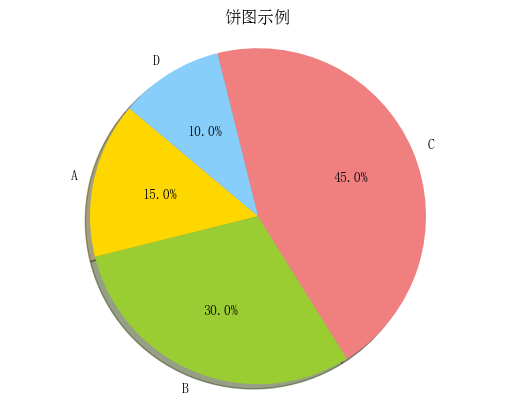
\includegraphics[width=0.6\textwidth]{part/图形化/Matplotlib/pic/绘图/饼图示例.png}
    \caption{饼图示例}
\end{figure}
\begin{lstlisting}[style=pythonstyle]
import matplotlib.pyplot as plt
labels = ['English', 'Maths', 'Chemistry']
scores = [90, 75, 88]
explode = (0, 0, 0.1) # 突出显示Chemistry
plt.pie(scores, explode=explode, labels=labels,
        autopct='%1.1f%%', shadow=True, startangle=60)
plt.axis('equal')
plt.legend(loc="upper right")
plt.title('学科成绩比例(突出显示Chemistry)')
plt.show()
\end{lstlisting}    
\begin{figure}[htpb]
    \centering
    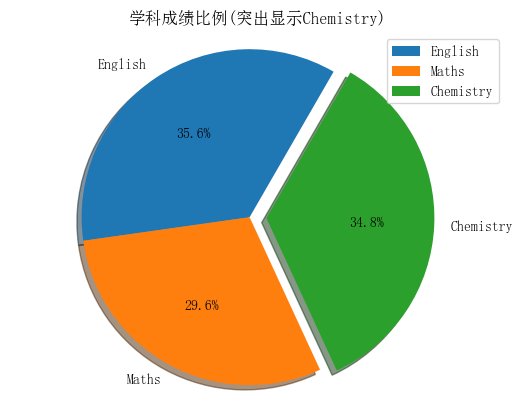
\includegraphics[width=0.6\textwidth]{part/图形化/Matplotlib/pic/绘图/学科成绩比例(突出显示Chemistry).png}
    \caption{学科成绩比例(突出显示Chemistry)}
\end{figure}

\begin{lstlisting}[style=pythonstyle]
import numpy as np
import matplotlib.pyplot as plt
import pandas as pd
plt.rcParams['font.sans-serif'] = 'SimHei'  # 设置中文显示
plt.rcParams['axes.unicode_minus'] = False

# 读取数据
data = pd.read_csv('../data/people.csv')
name = data.columns  # 提取其中的columns字段，视为数据的标签
values = data.values  # 提取其中的values字段，数据的存在位置
label = ['0-14岁人口', '15-64岁人口', '65岁及以上人口']  # 刻度标签
plt.figure(figsize=(6, 6))      # 将画布设定为正方形，则绘制的饼图是正圆

# 绘制饼图
explode = [0.01, 0.01, 0.01]    # 设定各项离心n个半径
plt.pie(values[-1, 2:5], explode=explode, labels=label, autopct='%1.1f%%')  
# values[-1, 2:5] 代表最后一行的第2、3、4列数据
# explode=explode 代表各项离心n个半径
# labels=label 代表各项标签
# autopct='%1.1f%%' 代表数值保留固定小数位

plt.title('2019年各年龄段年末总人口饼图')  # 添加图表标题
plt.savefig('../tmp/2019年各年龄段年末总人口饼图.png')
plt.show()
\end{lstlisting}
\begin{figure}[htpb]
    \centering
    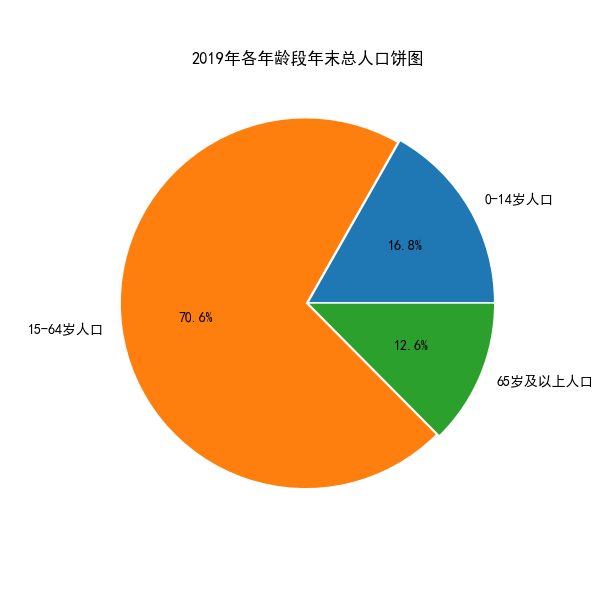
\includegraphics[width=0.4\textwidth]{part/图形化/Matplotlib/pic/绘图/2019年各年龄段年末总人口饼图.png}
    \caption{2019年各年龄段年末总人口饼图}
    \label{fig:2019年各年龄段年末总人口饼图}
\end{figure}





\section{boxplot 箱线图}
\codeinline{plt.boxplot()} 用于绘制箱线图。
\begin{lstlisting}[style=demostyle,numbers=none]
# 必须导入的库
import matplotlib.pyplot as plt
# boxplot 功能：绘制箱线图
plt.boxplot(x, notch=None, vert=None, patch_artist=None, widths=None, **kwargs)
# 参数说明：
# x : 数据
# notch : 是否为凹槽形
# vert : 是否垂直显示
# patch_artist : 是否填充箱体
# widths : 箱体的宽度
\end{lstlisting}
\begin{lstlisting}[style=pythonstyle]
import matplotlib.pyplot as plt
import numpy as np

# 数据
np.random.seed(10)
data = [np.random.normal(0, std, 100) for std in range(1, 4)]

# 绘制箱线图
plt.boxplot(data, vert=True, patch_artist=True, labels=['A', 'B', 'C'])
plt.title('箱线图')
plt.show()
\end{lstlisting}
\begin{figure}[htpb]
    \centering
    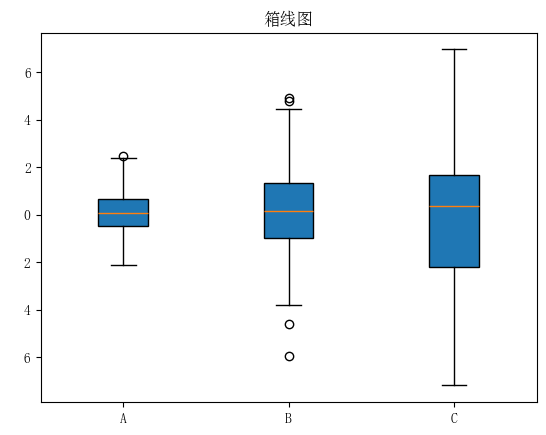
\includegraphics[width=0.6\textwidth]{part/图形化/Matplotlib/pic/绘图/箱型图演示.png}
    \caption{箱型图演示}
    \label{fig:箱型图演示}
\end{figure}

\begin{lstlisting}[style=pythonstyle]
import numpy as np
import matplotlib.pyplot as plt
import pandas as pd
plt.rcParams['font.sans-serif'] = 'SimHei'  # 设置中文显示
plt.rcParams['axes.unicode_minus'] = False
data = pd.read_csv('../data/people.csv')
name = data.columns  # 提取其中的columns字段，视为数据的标签
values = data.values  # 提取其中的values字段，数据的存在位置


label= ['0-14岁人口', '15-64岁人口', '65岁及以上人口']  # 定义标签
gdp = (list(values[:, 2]), list(values[:, 3]), list(values[:, 4]))
plt.figure(figsize=(7, 6))

# 绘制箱线图
plt.boxplot(gdp, notch=True, labels=label, meanline=True)
# notch=True 代表箱体是否为凹槽形
# labels=label 代表各项标签
# meanline=True 代表是否显示均值线

plt.title('2000-2019年各年龄段年末总人口箱线图')
plt.savefig('../tmp/2000-2019年各年龄段年末总人口箱线图.png')
plt.show()
\end{lstlisting}
\begin{figure}[htpb]
    \centering
    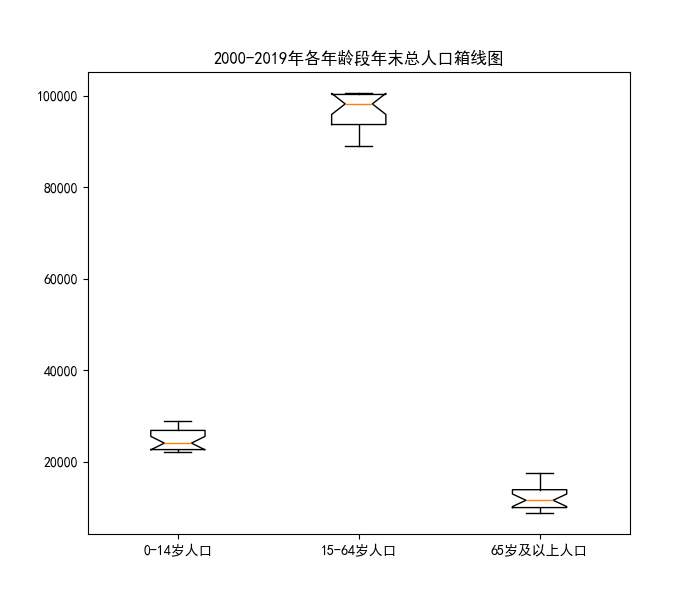
\includegraphics[width=0.4\textwidth]{part/图形化/Matplotlib/pic/绘图/2000-2019年各年龄段年末总人口箱线图.png}
    \caption{2000-2019年各年龄段年末总人口箱线图}
    \label{fig:2000-2019年各年龄段年末总人口箱线图}
\end{figure}



\section{直方图}
\subsection{plt.hist 一维频率直方图}
\begin{lstlisting}[style=demostyle,numbers=none]
# 必须导入的库
import matplotlib.pyplot as plt
# hist 功能：绘制一维频率直方图
plt.hist(x, bins=None, density=None, **kwargs)
# 参数说明：
# x : 数据
# bins : 分箱的数量或位置
# density : 是否显示概率密度
\end{lstlisting}
\codeinline{plt.hist()} 用于绘制一维频率直方图。
\begin{lstlisting}[style=pythonstyle]
import matplotlib.pyplot as plt
import numpy as np

# 数据
data = np.random.randn(1000)

# 绘制一维频率直方图
plt.hist(data, bins=30, alpha=0.7, color='blue')
plt.title('一维频率直方图')
plt.show()
\end{lstlisting}
\begin{figure}[htpb]
    \centering
    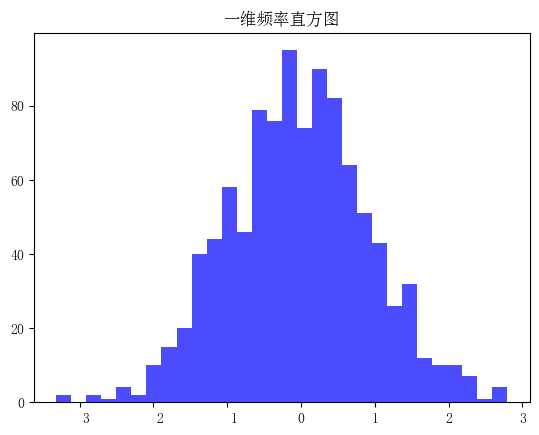
\includegraphics[width=0.6\textwidth]{part/图形化/Matplotlib/pic/绘图/一维频率直方图.png}
    \caption{一维频率直方图}
\end{figure}

\begin{lstlisting}[style=pythonstyle]
import matplotlib.pyplot as plt
import numpy as np

# 生成随机数据
data = np.random.randn(1000)

# 创建图像和子图
plt.figure(figsize=(8, 4))

# 第一个子图：histtype='step'
plt.subplot(1, 2, 1)
plt.title('step')
plt.hist(data, bins=50, density=True, alpha=1,  # density=True 代替旧的 normed=True
         histtype='step', color='grey', edgecolor='black')  # 线条模式，不填充

# 第二个子图：histtype='stepfilled'
plt.subplot(1, 2, 2)
plt.title('stepfilled')
plt.hist(data, bins=50, density=True, alpha=1, 
         histtype='stepfilled', color='grey', edgecolor='none')  # 填充的模式

# 调整布局并显示图像
plt.tight_layout()
plt.show()
\end{lstlisting}

\begin{figure}[htpb]
    \centering
    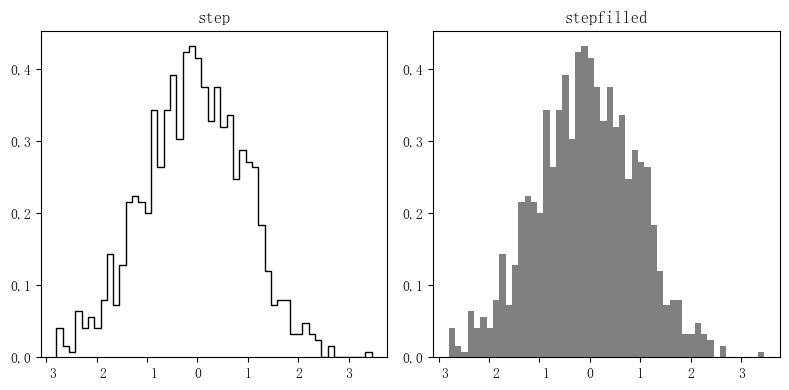
\includegraphics[width=0.6\textwidth]{part/图形化/Matplotlib/pic/绘图/不同histtype类型的直方图.png}
    \caption{不同histtype类型的直方图}
\end{figure}

stepfilled 与透明性参数 alpha 搭配使用的效果非常好：
\begin{lstlisting}[style=pythonstyle]
import matplotlib.pyplot as plt
import numpy as np

# 生成随机数据
x1 = np.random.normal(0, 2, 1000)    # 均值为0，标准差为2的正态分布
x2 = np.random.normal(-2, 1, 1000)   # 均值为-2，标准差为1的正态分布
x3 = np.random.normal(2, 2, 1000)    # 均值为2，标准差为2的正态分布

# 设置直方图的样式参数
kwargs = dict(histtype='stepfilled', alpha=0.5, density=True, bins=40)

# 创建图像
plt.figure(figsize=(8, 4))

# 绘制直方图
plt.hist(x1, **kwargs, color='blue', label='x1')  # 第一个数据集
plt.hist(x2, **kwargs, color='orange', label='x2')  # 第二个数据集
plt.hist(x3, **kwargs, color='green', label='x3')  # 第三个数据集

# 添加图例
plt.legend()

# 显示图像
plt.title('不同透明度的频次直方图')
plt.show()
\end{lstlisting}
\begin{figure}[htpb]
    \centering
    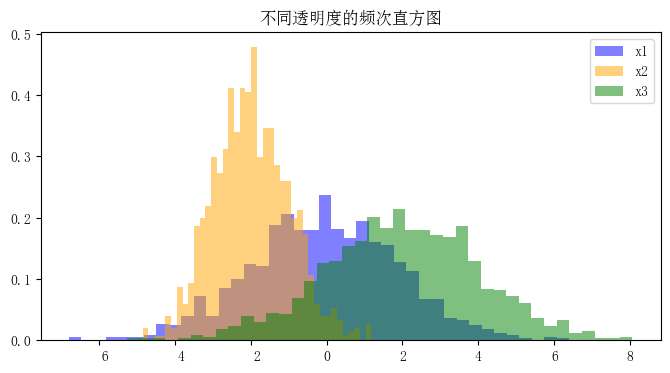
\includegraphics[width=0.6\textwidth]{part/图形化/Matplotlib/pic/绘图/不同透明度的频次直方图.png}
    \caption{不同透明度的频次直方图}
\end{figure}



\subsection{plt.hist2d 二维频率直方图}
\codeinline{plt.hist2d()} 用于绘制二维频率直方图。
\begin{lstlisting}[style=demostyle,numbers=none]
# 必须导入的库
import matplotlib.pyplot as plt
# hist2d 功能：绘制二维频率直方图
plt.hist2d(x, y, bins=10, range=None, density=False, cmap=None, **kwargs)
# 参数说明：
# x : x坐标
# y : y坐标
# bins : 分箱数
# range : x 和 y 的值范围
# density : 是否归一化
# cmap : 颜色映射
\end{lstlisting}
\begin{lstlisting}[style=pythonstyle]
import matplotlib.pyplot as plt
import numpy as np

# 数据
x = np.random.randn(1000)
y = np.random.randn(1000)

# 绘制二维频率直方图
plt.hist2d(x, y, bins=30, cmap='Blues')
plt.colorbar()
plt.title('二维频率直方图')
plt.show()
\end{lstlisting}
\begin{figure}[htpb]
    \centering
    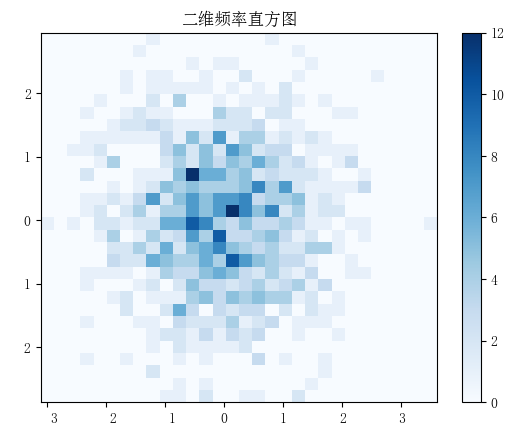
\includegraphics[width=0.6\textwidth]{part/图形化/Matplotlib/pic/绘图/二维频率直方图.png}
    \caption{二维频率直方图}
\end{figure}


\subsection{plt.hexbin 六边形区间划分}
二维频次直方图是由与坐标轴正交的方块分割而成的， 还有一种常用的方式是用正六边形分割。
\codeinline{plt.hexbin()} 用于绘制六边形区间划分。
\begin{lstlisting}[style=demostyle,numbers=none]
# 必须导入的库
import matplotlib.pyplot as plt
# hexbin 功能：绘制六边形分箱图
plt.hexbin(x, y, gridsize=30, cmap=None, **kwargs)
# 参数说明：
# x : x坐标
# y : y坐标
# gridsize : 网格大小
# cmap : 颜色映射
\end{lstlisting}
\begin{lstlisting}[style=pythonstyle]
import matplotlib.pyplot as plt
import numpy as np

# 数据
x = np.random.randn(10000)
y = np.random.randn(10000)

# 绘制六边形区间划分
plt.hexbin(x, y, gridsize=30, cmap='Greens')
plt.colorbar()
plt.title('六边形区间划分')
plt.show()
\end{lstlisting}
\begin{figure}[htpb]
    \centering
    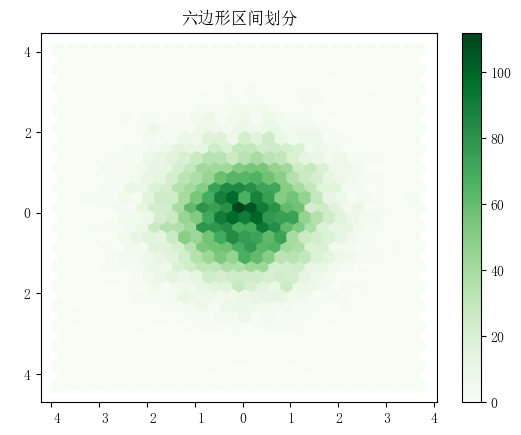
\includegraphics[width=0.6\textwidth]{part/图形化/Matplotlib/pic/绘图/六边形区间划分.png}
    \caption{六边形区间划分}
\end{figure}


\section{imshow热力图}
\codeinline{plt.imshow()} 用于绘制热力图。
\begin{lstlisting}[style=demostyle,numbers=none]
# 必须导入的库
import matplotlib.pyplot as plt
# imshow 功能：显示图像数据
plt.imshow(X, cmap=None, interpolation=None, **kwargs)
# 参数说明：
# X : 图像数据
# cmap : 颜色映射
# interpolation : 插值方法
## 'nearest'：最近邻插值
## 'bilinear'：双线性插值
## 'bicubic'：双三次插值
\end{lstlisting}
\begin{lstlisting}[style=pythonstyle]
import matplotlib.pyplot as plt
import numpy as np

# 数据
data = np.random.rand(10, 10)

# 绘制热力图
plt.imshow(data, cmap='hot', interpolation='nearest')
plt.colorbar()
plt.title('热力图')
plt.show()
\end{lstlisting}

\section{等高线图}
\subsection{plt.contour 等高线图}
\codeinline{plt.contour()} 用于绘制等高线图。
\begin{lstlisting}[style=demostyle,numbers=none]
# 必须导入的库
import matplotlib.pyplot as plt
# contour 功能：绘制等高线图
plt.contour(X, Y, Z, levels=None, colors=None, **kwargs)
# 参数说明：
# X, Y : 网格坐标
# Z : 等高线数据
# levels : 等高线的层次
# colors : 线条颜色
\end{lstlisting}
\begin{lstlisting}[style=pythonstyle]
import matplotlib.pyplot as plt
import numpy as np

# 数据
x = np.linspace(-3.0, 3.0, 100)
y = np.linspace(-3.0, 3.0, 100)
X, Y = np.meshgrid(x, y)
Z = np.exp(-X**2 - Y**2)

# 绘制等高线图
plt.contour(X, Y, Z, levels=10, cmap='viridis') # levels=10 表示等高线的数量 cmaps='viridis' 表示颜色
plt.title('等高线图')
plt.show()
\end{lstlisting}
\begin{figure}[htpb]
    \centering
    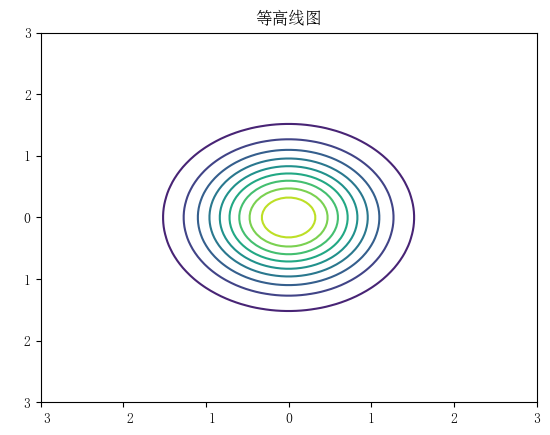
\includegraphics[width=0.6\textwidth]{part/图形化/Matplotlib/pic/绘图/等高线图-level10camaps=viridis.png}
    \caption{level=10,camaps=viridis的等高线图}
\end{figure}

\begin{lstlisting}[style=pythonstyle]
import matplotlib.pyplot as plt
import numpy as np

# 定义函数 f(x, y)
def f(x, y):
    return np.sin(x) ** 10 + np.cos(10 + y * x)

# 设置绘图风格
# plt.style.use('seaborn-v0_8-white')
plt.rcParams['font.family'] = 'SimSun'   

# 生成数据
x = np.linspace(0, 5, 50)
y = np.linspace(0, 5, 40)
X, Y = np.meshgrid(x, y)
Z = f(X, Y)

# 绘制等高线图
plt.contour(X, Y, Z, colors='black')

# 显示图像
plt.title('等高线图')
plt.show()
\end{lstlisting}

\begin{figure}[htpb]
    \centering
    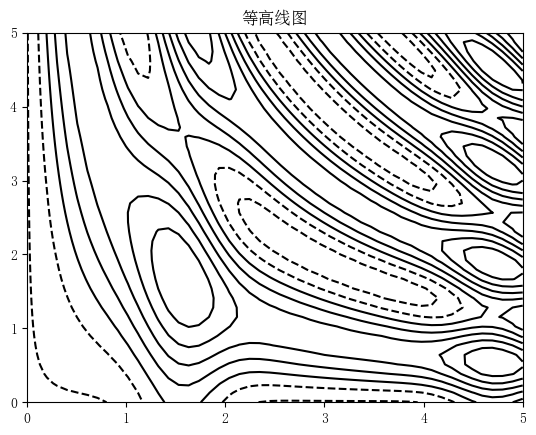
\includegraphics[width=0.6\textwidth]{part/图形化/Matplotlib/pic/绘图/实线和虚线是通过默认的等高线分布自动生成的.png}
    \caption{实线和虚线是通过默认的等高线分布自动生成的}
\end{figure}

实线：通常表示正值等高线的部分，代表函数在这些区域内的高度（或值）大于某一基准值。

虚线：通常表示负值等高线的部分，代表函数在这些区域内的高度（或值）小于某一基准值。

\begin{lstlisting}[style=pythonstyle]
import matplotlib.pyplot as plt
import numpy as np

# 定义函数 f(x, y)
def f(x, y):
    return np.sin(x) ** 10 + np.cos(10 + y * x)

# 生成数据
x = np.linspace(0, 5, 50)
y = np.linspace(0, 5, 40)
X, Y = np.meshgrid(x, y)
Z = f(X, Y)

# 绘制等高线图，并等分为20份，使用copper颜色方案
plt.contour(X, Y, Z, 20, cmap='copper')

# 显示图像
plt.title('使用copper色彩方案的等高线图')
plt.show()
\end{lstlisting}
\begin{figure}[htpb]
    \centering
    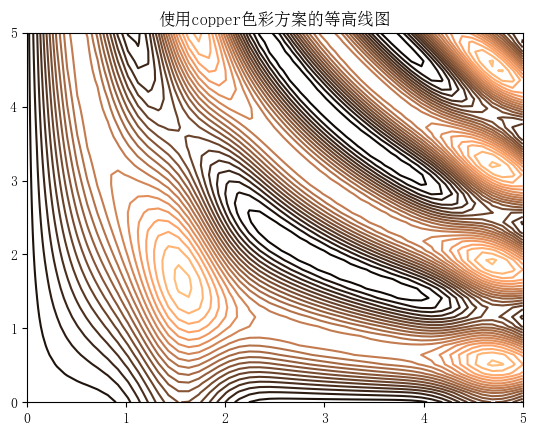
\includegraphics[width=0.6\textwidth]{part/图形化/Matplotlib/pic/绘图/使用copper色彩方案的等高线图.png}
    \caption{使用copper色彩方案的等高线图}
\end{figure}




\subsection{plt.contourf 带填充色的等高线图}
\codeinline{plt.contourf()} 用于绘制带填充色的等高线图。
\begin{lstlisting}[style=demostyle,numbers=none]
# 必须导入的库
import matplotlib.pyplot as plt
# contourf 功能：绘制填充的等高线图
plt.contourf(X, Y, Z, levels=None, cmap=None, **kwargs)
# 参数说明：
# X, Y : 网格坐标
# Z : 等高线数据
# levels : 等高线的层次
# cmap : 颜色映射
\end{lstlisting}
\begin{lstlisting}[style=pythonstyle]
import matplotlib.pyplot as plt
import numpy as np

# 定义函数 f(x, y)
def f(x, y):
    return np.sin(x) ** 10 + np.cos(10 + y * x)

# 生成数据
x = np.linspace(0, 5, 50)
y = np.linspace(0, 5, 40)
X, Y = np.meshgrid(x, y)
Z = f(X, Y)

# 绘制填充的等高线图，并等分为20份，使用copper颜色方案
plt.contourf(X, Y, Z, 20, cmap='copper')

# 添加颜色条
plt.colorbar()

# 显示图像
plt.title('颜色填充的等高线图')
plt.show()
\end{lstlisting}
\begin{figure}[htpb]
    \centering
    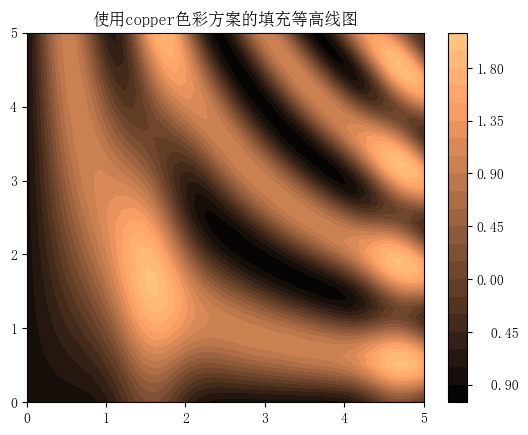
\includegraphics[width=0.6\textwidth]{part/图形化/Matplotlib/pic/绘图/颜色填充的等高线图.png}
    \caption{颜色填充的等高线图}
    \label{fig:颜色填充的等高线图}
\end{figure}

\begin{lstlisting}[style=pythonstyle]
import matplotlib.pyplot as plt
import numpy as np

# 定义函数 f(x, y)
def f(x, y):
    return np.sin(x) ** 10 + np.cos(10 + y * x)

# 生成数据
x = np.linspace(0, 5, 50)
y = np.linspace(0, 5, 40)
X, Y = np.meshgrid(x, y)
Z = f(X, Y)

# 绘制填充的等高线图，使用 hot 颜色方案，透明度为 0.75
plt.contourf(X, Y, Z, 20, alpha=0.75, cmap='hot')

# 画等高线，设置为黑色，线宽为 0.5
contours = plt.contour(X, Y, Z, 5, colors='black', linewidths=0.5)

# 为等高线添加标签
plt.clabel(contours, inline=True, fontsize=10)

# 添加颜色条
plt.colorbar()

# 显示图像
plt.title('使用 hot 色彩方案并添加标签的等高线图')
plt.show()
\end{lstlisting}
\begin{figure}[htpb]
    \centering
    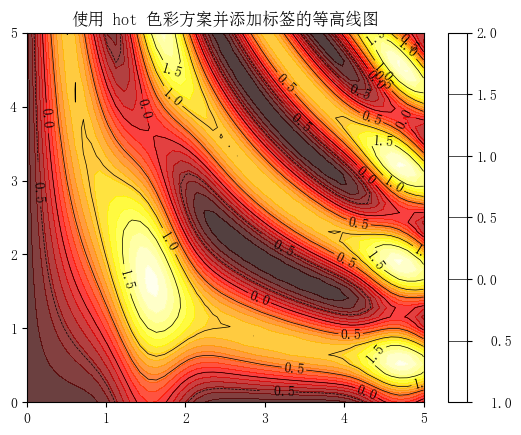
\includegraphics[width=0.6\textwidth]{part/图形化/Matplotlib/pic/绘图/使用hot色彩方案并添加标签的等高线图.png}
    \caption{使用hot色彩方案并添加标签的等高线图}
\end{figure}


\section{三维图}
Matplotlib 原本只能画2D图，后来扩展了 mplot3d 工具箱，它用来画三维图。
\begin{lstlisting}[style=demostyle,numbers=none]
from mpl_toolkits import mplot3d
# 或
from mpl_toolkits.mplot3d import Axes3D
\end{lstlisting} 

\subsection{plt.plot3D 三维数据点与线}
\codeinline{plt.plot3D()} 用于绘制三维数据点与线。
\begin{lstlisting}[style=demostyle,numbers=none]
# 必须导入的库
import matplotlib.pyplot as plt
from mpl_toolkits.mplot3d import Axes3D
# plot3D 功能：绘制三维数据点与线
plt.plot3D(x, y, z, color=None, **kwargs)
# 参数说明：
# x, y, z : 三维坐标
# color : 线条颜色
\end{lstlisting}
\begin{lstlisting}[style=pythonstyle]
import matplotlib.pyplot as plt
import numpy as np
from mpl_toolkits.mplot3d import Axes3D

# 数据
z = np.linspace(0, 1, 100)
x = z * np.sin(25 * z)
y = z * np.cos(25 * z)

# 绘制三维数据点与线
fig = plt.figure()
ax = fig.add_subplot(111, projection='3d')
ax.plot3D(x, y, z, 'gray')
plt.title(r'三维数据点与线 $x=z \cdot \sin(25z)$, $y=z \cdot \cos(25z)$')
plt.show()
\end{lstlisting}
\begin{figure}[htpb]
    \centering
    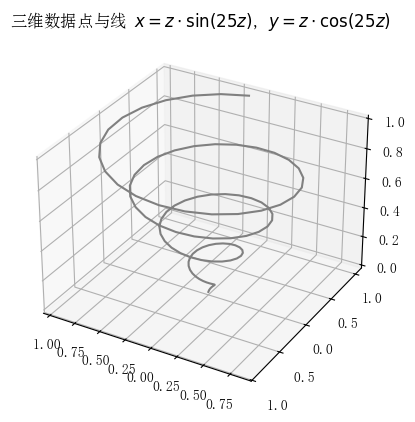
\includegraphics[width=0.6\textwidth]{part/图形化/Matplotlib/pic/绘图/三维数据点与线演示1.png}
    \caption{三维数据点与线 $x=z \cdot \sin(25z)$, $y=z \cdot \cos(25z)$}
    \label{fig:三维数据点与线演示1}
\end{figure}


\subsection{plt.contour3D 三维等高线图}
\codeinline{plt.contour3D()} 用于绘制三维等高线图。
\begin{lstlisting}[style=demostyle,numbers=none]
# 必须导入的库
import matplotlib.pyplot as plt
from mpl_toolkits.mplot3d import Axes3D
# contour3D 功能：绘制三维等高线图
plt.contour3D(X, Y, Z, levels=None, cmap=None, **kwargs)
# 参数说明：
# X, Y, Z : 三维网格数据
# levels : 等高线层数
# cmap : 颜色映射
\end{lstlisting}
\begin{lstlisting}[style=demostyle,numbers=none]
# contour3D()函数用法
ax.contour3D(X, Y, Z, 50, cmap='binary')
\end{lstlisting}

\begin{lstlisting}[style=pythonstyle]
import matplotlib.pyplot as plt
import numpy as np
from mpl_toolkits.mplot3d import Axes3D

# 数据
x = np.linspace(-3, 3, 100)
y = np.linspace(-3, 3, 100)
X, Y = np.meshgrid(x, y)
Z = np.sin(np.sqrt(X**2 + Y**2))

# 绘制三维等高线图
fig = plt.figure()
ax = fig.add_subplot(111, projection='3d')
ax.contour3D(X, Y, Z, 50, cmap='binary')
plt.title('三维等高线图')
plt.show()
\end{lstlisting}

\begin{lstlisting}[style=pythonstyle]
import matplotlib.pyplot as plt
import numpy as np
from mpl_toolkits.mplot3d import Axes3D

# 定义数据
x = np.linspace(-6, 6, 50)
y = np.linspace(-6, 6, 50)
X, Y = np.meshgrid(x, y)
Z = np.sin(np.sqrt(X**2 + Y**2))

# 定义绘图函数
def draw(ax, X, Y, Z):
    ax.contour3D(X, Y, Z, 40, cmap='hot')
    ax.set_xlabel('x')
    ax.set_ylabel('y')
    ax.set_zlabel('z')

# 创建图形和子图
fig = plt.figure(figsize=(10, 8))

# 第一个子图，默认视角
ax1 = fig.add_subplot(2, 2, 1, projection='3d')
draw(ax1, X, Y, Z)

# 第二个子图，调整俯仰角和方位角
ax2 = fig.add_subplot(2, 2, 2, projection='3d')
draw(ax2, X, Y, Z)
ax2.view_init(60, 35)  # 调整俯仰角为60度，方位角为35度

# 第三个子图，调整为俯视角度
ax3 = fig.add_subplot(2, 2, 3, projection='3d')
draw(ax3, X, Y, Z)
ax3.view_init(-90, 0)  # 调整俯仰角为-90度

# 第四个子图，反向视角
ax4 = fig.add_subplot(2, 2, 4, projection='3d')
draw(ax4, X, Y, Z)
ax4.view_init(-180, 35)  # 反方向，调整为-180度的俯仰角

# 调整布局并显示图像
plt.tight_layout()
plt.show()
\end{lstlisting}
\begin{figure}[htpb]
    \centering
    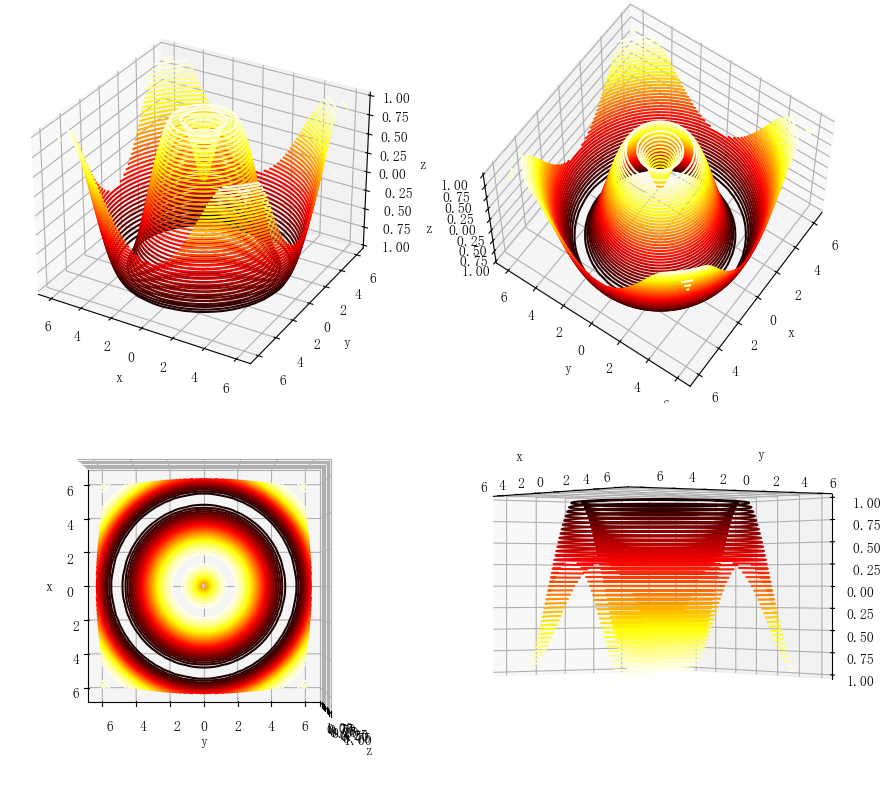
\includegraphics[width=0.8\textwidth]{part/图形化/Matplotlib/pic/绘图/3D等高线不同视图.png}
    \caption{3D等高线不同视图}
    \label{fig:3D等高线不同视图}
\end{figure}



\subsection{plt.plot\_wireframe 线框图}
\codeinline{plt.plot\_wireframe()} 用于绘制线框图。
\begin{lstlisting}[style=demostyle,numbers=none]
# 必须导入的库
import matplotlib.pyplot as plt
from mpl_toolkits.mplot3d import Axes3D
# plot_wireframe 功能：绘制线框图
plt.plot_wireframe(X, Y, Z, rstride=1, cstride=1, **kwargs)
# 参数说明：
# X, Y, Z : 网格数据
# rstride : 行步长
# cstride : 列步长
\end{lstlisting}
\begin{lstlisting}[style=pythonstyle]
import matplotlib.pyplot as plt
import numpy as np
from mpl_toolkits.mplot3d import Axes3D

# 数据
x = np.linspace(-5, 5, 50)
y = np.linspace(-5, 5, 50)
X, Y = np.meshgrid(x, y)
Z = np.sin(np.sqrt(X**2 + Y**2))

# 绘制线框图
fig = plt.figure()
ax = fig.add_subplot(111, projection='3d')
ax.plot_wireframe(X, Y, Z, color='black')
plt.title('线框图')
plt.show()
\end{lstlisting}
\begin{figure}[htpb]
    \centering
    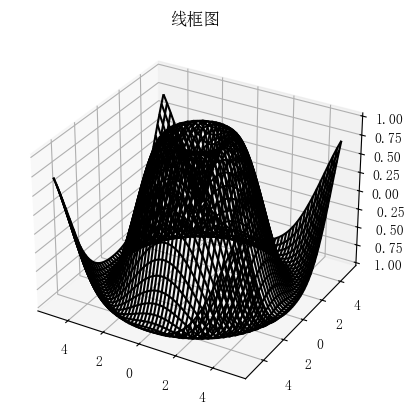
\includegraphics[width=0.6\textwidth]{part/图形化/Matplotlib/pic/绘图/线框图演示.png}
    \caption{线框图演示}
    \label{fig:线框图演示}
\end{figure}


\subsection{plt.plot\_surface 曲面图}
\codeinline{plt.plot\_surface()} 用于绘制曲面图。
\begin{lstlisting}[style=demostyle,numbers=none]
# 必须导入的库
import matplotlib.pyplot as plt
from mpl_toolkits.mplot3d import Axes3D
# plot_surface 功能：绘制曲面图
plt.plot_surface(X, Y, Z, cmap=None, **kwargs)
# 参数说明：
# X, Y, Z : 网格数据
# cmap : 颜色映射
\end{lstlisting}
\begin{lstlisting}[style=pythonstyle]
import matplotlib.pyplot as plt
import numpy as np
from mpl_toolkits.mplot3d import Axes3D

# 数据
x = np.linspace(-5, 5, 50)
y = np.linspace(-5, 5, 50)
X, Y = np.meshgrid(x, y)
Z = np.sin(np.sqrt(X**2 + Y**2))

# 绘制曲面图
fig = plt.figure()
ax = fig.add_subplot(111, projection='3d')
ax.plot_surface(X, Y, Z, cmap='viridis')
plt.title('曲面图')
plt.show()
\end{lstlisting}
\begin{figure}[htpb]
    \centering
    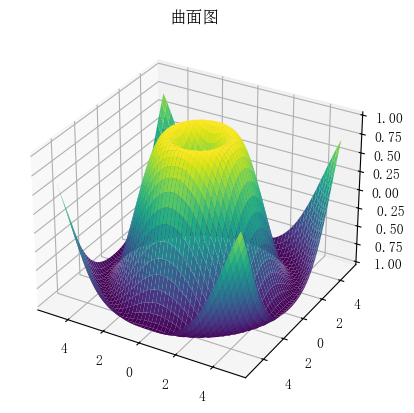
\includegraphics[width=0.6\textwidth]{part/图形化/Matplotlib/pic/绘图/曲面图演示.png}
    \caption{曲面图演示}
    \label{fig:曲面图演示}
\end{figure}

\begin{example}
    \exProblem
    绘制函数 $f(x, y) = (x^2 + y^2)\sin\left(\frac{1}{x^2 + y^2}\right)$ 的三维曲面图。

    \exSolution
\begin{lstlisting}[style=pythonstyle]    
import numpy as np
import matplotlib.pyplot as plt
from mpl_toolkits.mplot3d import Axes3D

# 定义函数 f(x, y)
def f(x, y):
    with np.errstate(divide='ignore', invalid='ignore'):
        z = (x**2 + y**2) * np.sin(1 / (x**2 + y**2))
        z[np.isnan(z)] = 0  # 处理 x^2 + y^2 = 0 的情况，避免除以零
        z[np.isinf(z)] = 0  # 处理无穷大的情况
    return z

# 创建 x 和 y 的网格数据
x = np.linspace(-1, 1, 300)
y = np.linspace(-1, 1, 300)
X, Y = np.meshgrid(x, y)

# 计算函数值
Z = f(X, Y)

# 创建三维图像
fig = plt.figure(figsize=(10, 8))
ax = fig.add_subplot(111, projection='3d')

# 绘制三维曲面图
surf = ax.plot_surface(X, Y, Z, cmap='viridis')

# 添加颜色条
fig.colorbar(surf, ax=ax, shrink=0.5, aspect=5)

# 设置标题和标签
ax.set_title(r'$f(x, y) = (x^2 + y^2)\sin\left(\frac{1}{x^2 + y^2}\right)$')
ax.set_xlabel('X axis')
ax.set_ylabel('Y axis')
ax.set_zlabel('Z axis')

# 显示图像
plt.show()
\end{lstlisting}

\begin{figure}[htpb]
    \centering
    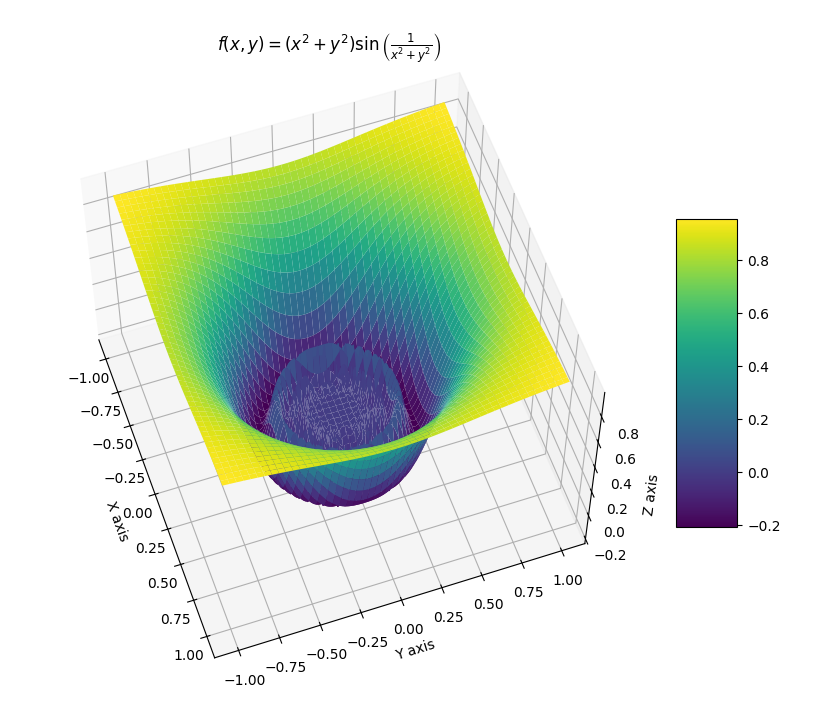
\includegraphics[width=0.6\textwidth]{part/图形化/Matplotlib/pic/绘图/曲面图surface_例题1.png}
    \caption{曲面图 $f(x, y) = (x^2 + y^2)\sin\left(\frac{1}{x^2 + y^2}\right)$}
    \label{fig:曲面图surface_例题1}
\end{figure}

\end{example}



\subsubsection{plt.plot\_surface 极坐标曲面图}
极坐标曲面图的绘制可以通过曲面的极坐标变换实现

\begin{lstlisting}[style=pythonstyle]
import matplotlib.pyplot as plt
import numpy as np
from mpl_toolkits.mplot3d import Axes3D

# 数据
r = np.linspace(0, 1, 50)
p = np.linspace(0, 2*np.pi, 50)
R, P = np.meshgrid(r, p)
Z = R**2

# 极坐标转化为笛卡尔坐标
X = R * np.cos(P)
Y = R * np.sin(P)

# 绘制极坐标曲面图
fig = plt.figure()
ax = fig.add_subplot(111, projection='3d')
ax.plot_surface(X, Y, Z, cmap='viridis')
plt.title('极坐标曲面图')
plt.show()
\end{lstlisting}

\subsubsection{plt.plot\_trisurf 曲面三角剖分}
\codeinline{plt.plot\_trisurf()} 用于绘制曲面三角剖分图。
\begin{lstlisting}[style=demostyle,numbers=none]
# 必须导入的库
import matplotlib.pyplot as plt
from mpl_toolkits.mplot3d import Axes3D
# plot_trisurf 功能：绘制曲面三角剖分
plt.plot_trisurf(x, y, z, cmap=None, **kwargs)
# 参数说明：
# x, y, z : 三维坐标
# cmap : 颜色映射
\end{lstlisting}
\begin{lstlisting}[style=pythonstyle]
import matplotlib.pyplot as plt
import numpy as np
from mpl_toolkits.mplot3d import Axes3D

# 数据
x = np.random.rand(100) * 10
y = np.random.rand(100) * 10
z = np.sin(np.sqrt(x**2 + y**2))

# 绘制曲面三角剖分图
fig = plt.figure()
ax = fig.add_subplot(111, projection='3d')
ax.plot_trisurf(x, y, z, cmap='viridis', edgecolor='none')
plt.title('曲面三角剖分')
plt.show()
\end{lstlisting}


\chapter{[matplotlib] 图片样式与排版}
\section{默认配置}
matplotlib 的相关配置主要包括以下几种，用户可以自定义它们：
\begin{enumerate}[label=\arabic*)]
    \item 图片大小(\codeinline{figsize})和分辨率(\codeinline{dpi})
    \item 线宽(\codeinline{linewidth})、颜色(\codeinline{color})、风格(\codeinline{linestyle})和标记(\codeinline{marker})
    \item 坐标轴(\codeinline{axis})、坐标轴标签(\codeinline{xlabel, ylabel})以及网格(\codeinline{grid})的属性
    \item 文字(\codeinline{text})与字体(\codeinline{font})属性。
\end{enumerate}

所有的默认属性均保存在 \codeinline{matplotlib.rcParams} 字典中。
\begin{lstlisting}[style=pythonstyle]
import matplotlib.pyplot as plt

# 查看所有的 rcParams 及其默认值
for key, value in plt.rcParams.items():
    print(f"{key}: {value}")
\end{lstlisting}    

可以对 \codeinline{plt.rcParams} 进行修改，以\textcolor{red}{\textbf{全局}}改变默认的配置。例如，修改图片的尺寸和分辨率：
\begin{lstlisting}[style=pythonstyle]
import matplotlib.pyplot as plt

# 查看特定的 rcParams 值
print(plt.rcParams['figure.figsize'])  # 图像尺寸
print(plt.rcParams['figure.dpi'])      # 图像分辨率
print(plt.rcParams['lines.linewidth']) # 线条宽度

# 修改默认的图像尺寸和分辨率
plt.rcParams['figure.figsize'] = [10, 6]
plt.rcParams['figure.dpi'] = 120
print(plt.rcParams['figure.figsize'])  # 图像尺寸
print(plt.rcParams['figure.dpi'])      # 图像分辨率

# 绘制一个简单的图形，使用新的设置
plt.plot([1, 2, 3, 4], [1, 4, 2, 3])
plt.show()
\end{lstlisting}   

如果不想全局修改默认配置，可以使用 \codeinline{plt.rc()} 函数来临时修改配置：
\begin{lstlisting}[style=pythonstyle]
import matplotlib.pyplot as plt  
plt.figure(figsize=(10, 6), dpi=120)  
plt.plot([1, 2, 3, 4], [1, 4, 2, 3])
plt.show()
\end{lstlisting}

\section{显示中文}
\begin{lstlisting}[style=demostyle,numbers=none]
# 1.定位matplotlib的字体库路径
import matplotlib
matplotlib.matplotlib_fname()
>>> '/home/changjie/.local/conda_env/pytorch_test/lib/python3.10/site-packages/matplotlib/mpl-data/matplotlibrc'

# 2.将中文字体文件**.ttf，拷贝到该目录的fonts/ttf下
cp /usr/share/fonts/emacs_cnfonts/chinese/* /home/changjie/.local/conda_env/pytorch_test/lib/python3.10/site-packages/matplotlib/mpl-data/fonts/ttf/

# 3删除 matplotlib 缓存
cd ~/.cache/matplotlib
rm * -r

# 4.查看是否成功
import matplotlib.pyplot as plt  
from matplotlib import font_manager  
# 获取字体管理器并列出所有TTF字体  
fonts = [f.name for f in font_manager.fontManager.ttflist]  
sorted_fonts = sorted(fonts)  
# 打印排序后的字体列表  
print(sorted_fonts)

# 5.使用字体
## 1)用plt.rcParams设置
plt.rcParams['font.family'] = 'SimSun'   
plt.rcParams['axes.unicode_minus'] = False  # 解决保存图像时负号'-'显示为方块的问题

## 2)用FontProperties，并指定字体文件
from matplotlib.font_manager import FontProperties
import matplotlib.pyplot as plt
font = FontProperties(fname='/mnt/share/code/font/SimHei.ttf', size=20)
plt.title('测试', fontproperties=font)
\end{lstlisting}  

\section{图片的属性}
\begin{table}[h]
    \centering
    \begin{tabular}{|c|c|l|}
    \hline
    \textbf{参数} & \textbf{默认值} & \textbf{描述}                 \\ \hline
    num           & 1               & 图像的数量                   \\ \hline
    figsize       & figure.figsize  & 图像的长和宽（英寸）         \\ \hline
    dpi           & figure.dpi      & 分辨率（像素/英寸）           \\ \hline
    facecolor     & figure.facecolor & 绘图区域的背景颜色           \\ \hline
    edgecolor     & figure.edgecolor & 绘图区域边缘的颜色           \\ \hline
    frameon       & True            & 是否绘制图像边缘             \\ \hline
    \end{tabular}
    \caption{图像的属性}
\end{table}

高 dpi 显示图像更细腻，但是图像尺寸也会变大。使用默认值即可。如果图像非常复杂，为了看清细节，我们可以调整宽高的英寸数。

\begin{lstlisting}[style=pythonstyle]
import matplotlib.pyplot as plt
plt.rcParams['font.family'] = 'SimSun'   

# 示例 1：默认参数
plt.figure(num=1)
plt.plot([0, 1, 2], [0, 1, 4], label='默认参数')
plt.title('默认参数')
plt.legend()
plt.show()

# 示例 2：设置图像大小（figsize）
plt.figure(num=2, figsize=(10, 5))
plt.plot([0, 1, 2], [0, 1, 4], label='figsize = (10, 5)')
plt.title('设置图像大小')
plt.legend()
plt.show()

# 示例 3：设置分辨率（dpi）
plt.figure(num=3, dpi=150)
plt.plot([0, 1, 2], [0, 1, 4], label='dpi = 150')
plt.title('设置分辨率')
plt.legend()
plt.show()

# 示例 4：设置背景颜色（facecolor）
plt.figure(num=4, facecolor='lightgray')
plt.plot([0, 1, 2], [0, 1, 4], label='facecolor = lightgray')
plt.title('设置背景颜色')
plt.legend()
plt.show()

# 示例 5：设置边缘颜色（edgecolor）
plt.figure(num=5, edgecolor='red')
plt.plot([0, 1, 2], [0, 1, 4], label='edgecolor = red')
plt.title('设置边缘颜色')
plt.legend()
plt.show()

# 示例 6：关闭边框（frameon=False）
plt.figure(num=6, frameon=False)
plt.plot([0, 1, 2], [0, 1, 4], label='frameon = False')
plt.title('关闭边框')
plt.legend()
plt.show()
\end{lstlisting}

\begin{figure}[htpb]
    \centering
    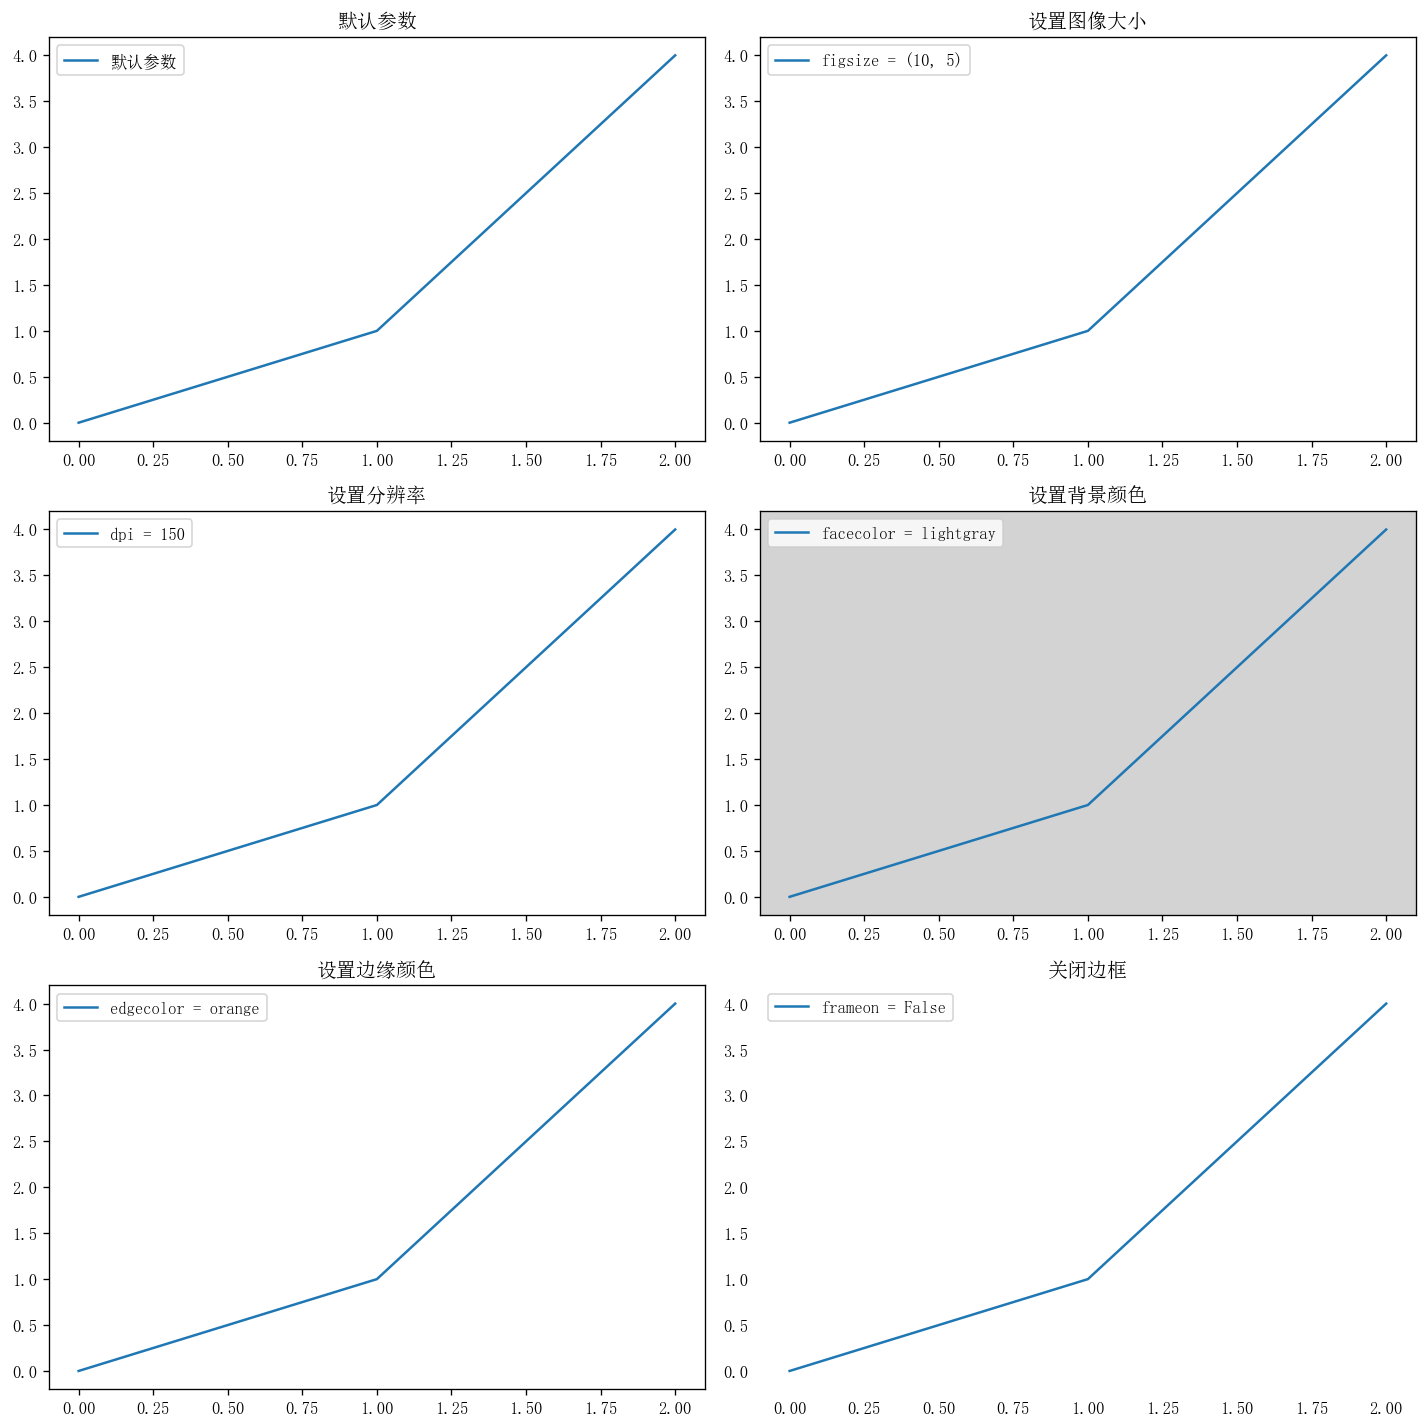
\includegraphics[width=0.8\textwidth]{part/图形化/Matplotlib/pic/图片样式与排版/修改图片参数.png}
    \caption{修改图片参数}
    \label{fig:修改图片参数}
\end{figure}

\section{matplotlib线条}
\subsection{线条的颜色}
matplotlib 支持使用以下缩写字符设置线条的颜色：

\begin{table}[h]
\centering
\caption{线条颜色}
\begin{tabular}{|c|c|}
\hline
\textbf{缩写字符} & \textbf{颜色} \\ \hline
\codeinline{'b'} & blue \\ \hline
\codeinline{'g'} & green \\ \hline
\codeinline{'r'} & red \\ \hline
\codeinline{'c'} & cyan \\ \hline
\codeinline{'m'} & magenta \\ \hline
\codeinline{'y'} & yellow \\ \hline
\codeinline{'k'} & black \\ \hline
\codeinline{'w'} & white \\ \hline
\end{tabular}
\end{table}

\begin{lstlisting}[style=pythonstyle]
import matplotlib.pyplot as plt

# 颜色列表
colors = ['b', 'g', 'r', 'c', 'm', 'y', 'k', 'w']
labels = ['blue', 'green', 'red', 'cyan', 'magenta', 'yellow', 'black', 'white']

plt.figure(figsize=(10, 6))
for i, color in enumerate(colors):
    plt.plot([0, 1, 2], [i, i + 1, i + 2], color=color, label=labels[i])

plt.title('线条的颜色')
plt.legend(loc='upper left')
plt.show()
\end{lstlisting}

\begin{figure}[htpb]
    \centering
    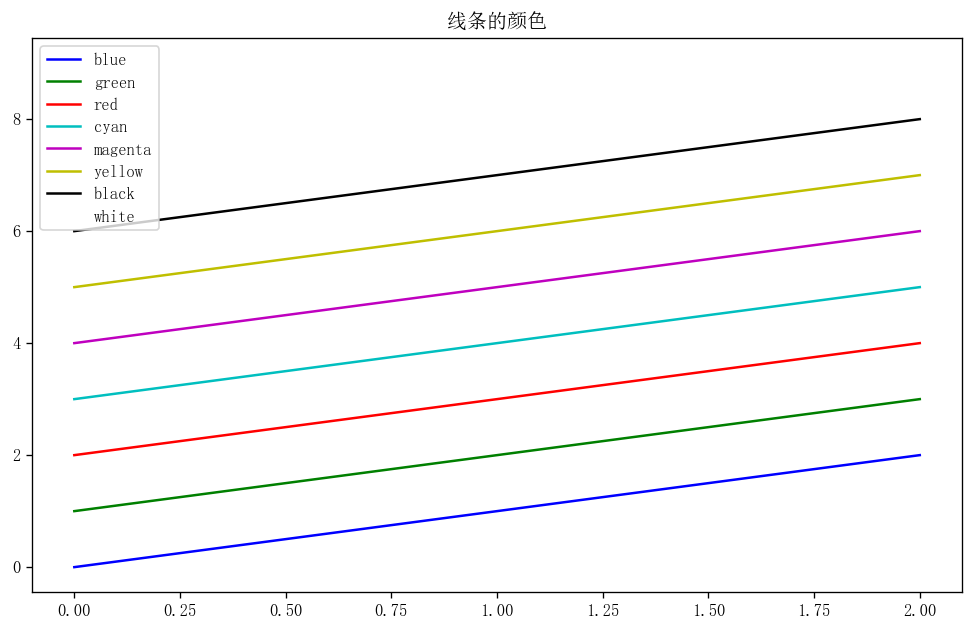
\includegraphics[width=0.6\textwidth]{part/图形化/Matplotlib/pic/图片样式与排版/线条-颜色.png}
    \caption{线条的颜色}
    \label{fig:线条的颜色}
\end{figure}


\subsection{线条的粗细}
线条的粗细可以通过 \codeinline{linewidth} 或 \codeinline{lw} 参数指定，取值为浮点数，表示线条的宽度点数。以下是不同 \codeinline{linewidth} 设置的示例：

\begin{lstlisting}[style=pythonstyle]
import matplotlib.pyplot as plt

# 线条粗细列表
linewidths = [0.5, 1.0, 1.5, 2.0, 2.5, 3.0]

plt.figure(figsize=(10, 6))
for i, lw in enumerate(linewidths):
    # 这里不指定颜色就是使用默认的颜色序列来绘制线条。
    plt.plot([0, 1, 2], [i, i + 1, i + 2], linewidth=lw, label=f'linewidth = {lw}')

plt.title('线条的粗细')
plt.legend(loc='upper left')
plt.show()
\end{lstlisting}

\begin{figure}[htpb]
    \centering
    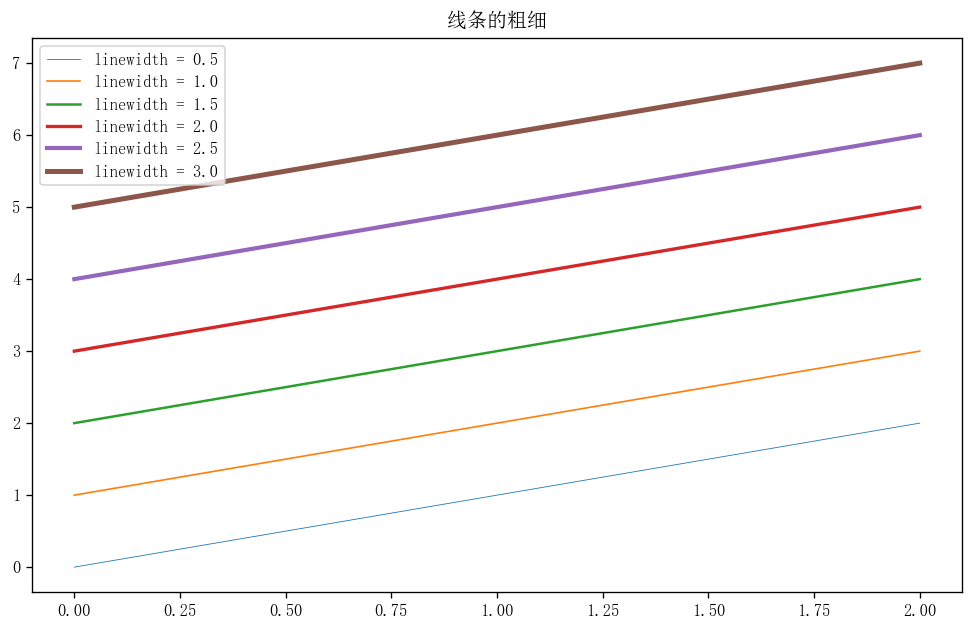
\includegraphics[width=0.6\textwidth]{part/图形化/Matplotlib/pic/图片样式与排版/线条-粗细.png}
    \caption{线条的粗细}
    \label{fig:线条的粗细}
\end{figure}


\subsection{线条的样式}
线条样式可以使用 \codeinline{linestyle} 或 \codeinline{ls} 参数来指定。支持的样式有以下几种：

\begin{table}[h]
\centering
\caption{线条样式}
\begin{tabular}{|c|l|}
\hline
\textbf{样式缩写} & \textbf{描述} \\ \hline
\codeinline{'-'}  & 实线 \\ \hline
\codeinline{'--'} & 短划线 \\ \hline
\codeinline{':' } & 点划线 \\ \hline
\codeinline{'-.'} & 虚线 \\ \hline
\end{tabular}
\end{table}

\begin{lstlisting}[style=pythonstyle]
import matplotlib.pyplot as plt

# 线条样式列表
linestyles = ['-', '--', ':', '-.']
labels = ['实线', '短划线', '点划线', '虚线']

plt.figure(figsize=(10, 6))
for i, ls in enumerate(linestyles):
    plt.plot([0, 1, 2], [i, i + 1, i + 2], linestyle=ls, label=labels[i])

plt.title('线条的样式')
plt.legend(loc='upper left')
plt.show()  
\end{lstlisting}

\begin{figure}[htpb]
    \centering
    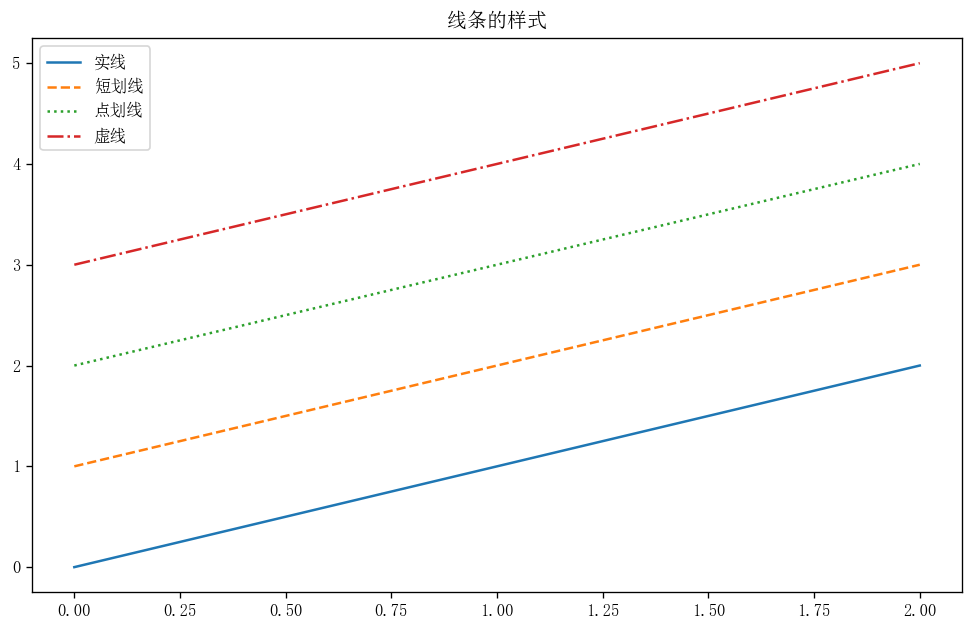
\includegraphics[width=0.6\textwidth]{part/图形化/Matplotlib/pic/图片样式与排版/线条-样式.png}
    \caption{线条的样式}
    \label{fig:线条的样式}
\end{figure}


\subsection{线条的标记}
线条标记是用来在图上标注数据点的符号，可以使用 \codeinline{marker} 参数指定。以下是常用的标记样式：

\begin{table}[h]
\centering
\caption{线条标记}
\begin{tabular}{|c|l|}
\hline
\textbf{标记缩写} & \textbf{描述} \\ \hline
\codeinline{'.'} & 点 (point marker) \\ \hline
\codeinline{','} & 像素 (pixel marker) \\ \hline
\codeinline{'o'} & 圆圈 (circle marker) \\ \hline
\codeinline{'v'} & 向下三角形 (triangle\_down marker) \\ \hline
\codeinline{\textasciicircum} & 向上三角形 (triangle\_up marker) \\ \hline
\codeinline{'<'} & 向左三角形 (triangle\_left marker) \\ \hline
\codeinline{'>'} & 向右三角形 (triangle\_right marker) \\ \hline
\codeinline{'1'} & 下三角 (tri\_down marker) \\ \hline
\codeinline{'2'} & 上三角 (tri\_up marker) \\ \hline
\codeinline{'3'} & 左三角 (tri\_left marker) \\ \hline
\codeinline{'4'} & 右三角 (tri\_right marker) \\ \hline
\codeinline{'s'} & 正方形 (square marker) \\ \hline
\codeinline{'p'} & 五边形 (pentagon marker) \\ \hline
\codeinline{'*'} & 星形 (star marker) \\ \hline
\codeinline{'h'} & 六边形1 (hexagon1 marker) \\ \hline
\codeinline{'H'} & 六边形2 (hexagon2 marker) \\ \hline
\codeinline{'+'} & 加号 (plus marker) \\ \hline
\codeinline{'x'} & 叉号 (x marker) \\ \hline
\codeinline{'D'} & 菱形 (diamond marker) \\ \hline
\codeinline{'d'} & 细菱形 (thin\_diamond marker) \\ \hline
\codeinline{'|'} & 竖线 (vline marker) \\ \hline
\codeinline{'$\_$'} & 横线 (hline marker) \\ \hline
\end{tabular}
\end{table}

\begin{lstlisting}[style=pythonstyle]
import matplotlib.pyplot as plt

# 标记样式列表
markers = ['.', ',', 'o', 'v', '^', '<', '>', '1', '2', '3', '4', 's', 'p', '*', 'h', 'H', '+', 'x', 'D', 'd', '|', '_']
labels = [
    'point', 'pixel', 'circle', 'triangle_down', 'triangle_up', 'triangle_left', 'triangle_right', 
    'tri_down', 'tri_up', 'tri_left', 'tri_right', 'square', 'pentagon', 'star', 'hexagon1', 
    'hexagon2', 'plus', 'x', 'diamond', 'thin_diamond', 'vline', 'hline'
]

plt.figure(figsize=(12, 8))
for i, marker in enumerate(markers):
    plt.plot([0, 1, 2], [i, i + 1, i + 2], marker=marker, label=labels[i])

plt.title('线条的标记')
plt.legend(loc='upper left', fontsize='small')
plt.show()
\end{lstlisting}

\begin{figure}[htpb]
    \centering
    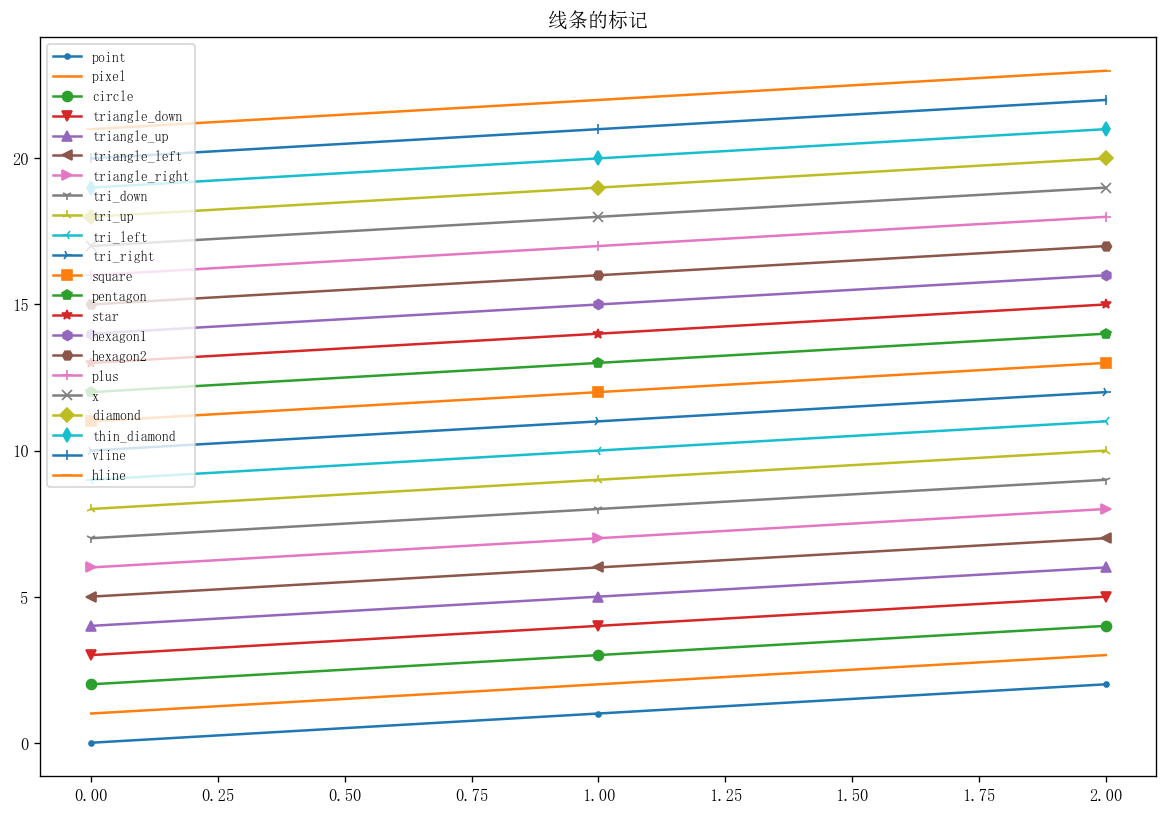
\includegraphics[width=0.6\textwidth]{part/图形化/Matplotlib/pic/图片样式与排版/线条-标记.png}
    \caption{线条的标记}
    \label{fig:线条的标记}
\end{figure}

\begin{lstlisting}[style=pythonstyle]
import matplotlib.pyplot as plt

# 定义标记样式和方向属性
markers = ['o', 'v', '^', '<', '>', '8', 's', 'p', '*', 'h', 'H', 'D', 'd', 'P', 'X']
fillstyles = ['full', 'left', 'right', 'bottom', 'top', 'none']  # 标记的填充样式

# 设置图像大小和子图网格
fig, axs = plt.subplots(len(markers), len(fillstyles), figsize=(12, 18))

# 循环绘制每种标记和填充样式
for i, marker in enumerate(markers):
    for j, fillstyle in enumerate(fillstyles):
        axs[i, j].plot(0, 0, marker=marker, markersize=20, markerfacecolor='orange', fillstyle=fillstyle)
        axs[i, j].set_xticks([])
        axs[i, j].set_yticks([])
        axs[i, j].set_xlim(-1, 1)
        axs[i, j].set_ylim(-1, 1)
        axs[i, j].text(0, 0, f"('{marker}',{fillstyle})", ha='center', va='center')

plt.tight_layout()
plt.show()
\end{lstlisting}


\section{图片的边界}
图片的边界可以通过 \codeinline{plt.xlim()} 和 \codeinline{plt.ylim()} 函数来设置。以下示例展示了如何设置图片的边界：

\begin{lstlisting}[style=pythonstyle]
import matplotlib.pyplot as plt
import numpy as np

# 创建数据
x = np.linspace(-np.pi, np.pi, 100)
y1 = np.sin(x)
y2 = np.cos(x)

# 创建两个子图用于比较
fig, (ax1, ax2) = plt.subplots(1, 2, figsize=(12, 6))

# 第一个子图：默认上下限
ax1.plot(x, y1, color='blue', label='sin(x)')
ax1.plot(x, y2, color='orange', label='cos(x)')
ax1.set_xlim(-np.pi, np.pi)  # 设置 x 轴的上下限
ax1.set_ylim(-1.0, 1.0)      # 设置 y 轴的上下限
ax1.set_title('原始图像')
ax1.legend()

# 第二个子图：扩展 y 轴的上下限 10%
ax2.plot(x, y1, color='blue', label='sin(x)')
ax2.plot(x, y2, color='orange', label='cos(x)')
ax2.set_xlim(-np.pi, np.pi)  # 设置 x 轴的上下限
ax2.set_ylim(-1.1, 1.1)      # 扩展 y 轴的上下限 10%
ax2.set_title('扩展 y 轴上下 10%')
ax2.legend()

# 调整布局并显示图像
plt.tight_layout()
plt.show()
\end{lstlisting}

\begin{figure}[htpb]
    \centering
    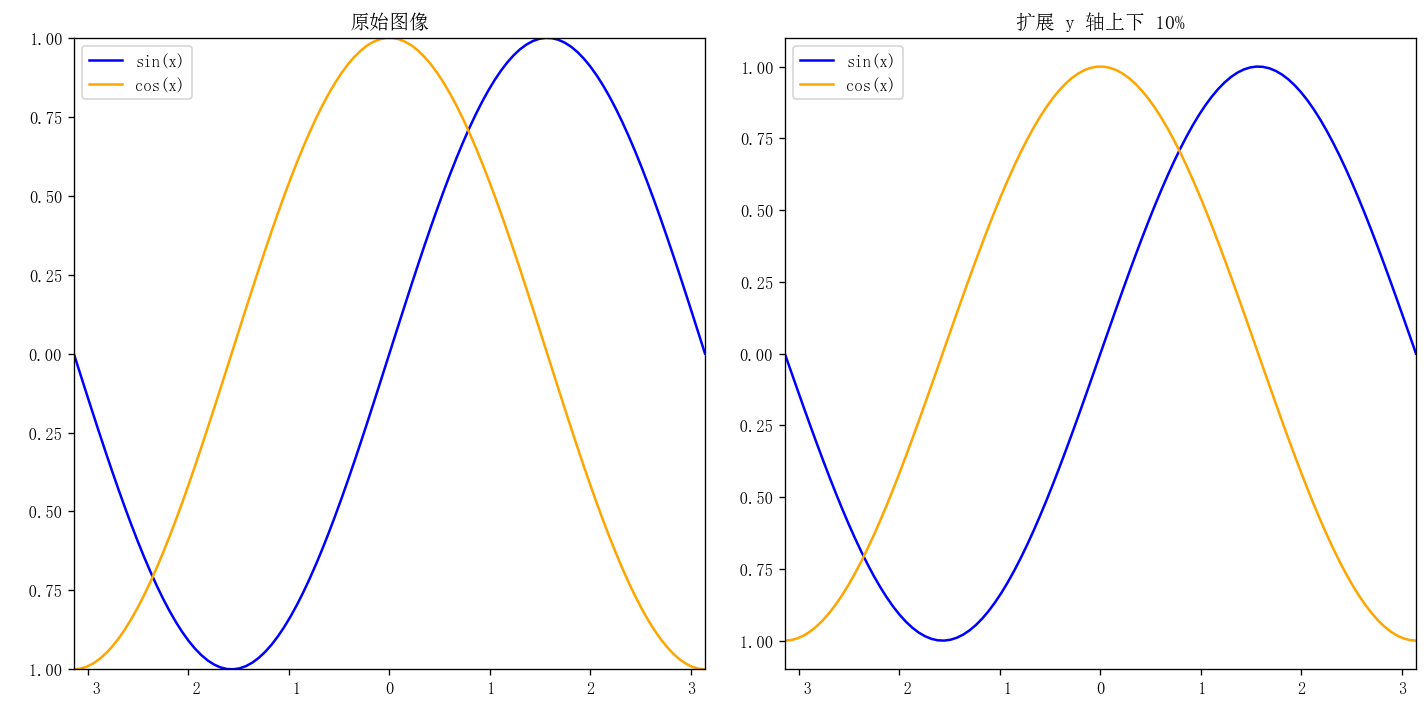
\includegraphics[width=0.6\textwidth]{part/图形化/Matplotlib/pic/图片样式与排版/图片的边界.png}
    \caption{图片的边界}
    \label{fig:图片的边界}
\end{figure}

\section{坐标轴}
\subsection{坐标记号标签}
坐标记号标签通过 \codeinline{plt.xticks()} 和 \codeinline{plt.yticks()} 函数来设置。
其主要功能包括：
\begin{enumerate}[label=\arabic*)]
    \item 设置刻度位置：指定 x 轴上显示刻度的位置。
    \item 设置刻度标签：自定义刻度位置的显示标签，可以使用字符串、数学符号等。
    \item 美化图表：通过设置刻度和标签，可以让图表看起来更加专业、易于理解。
\end{enumerate}

\begin{lstlisting}[style=pythonstyle]
import matplotlib.pyplot as plt
import numpy as np

# 数据
x = np.linspace(-np.pi, np.pi, 100)
y = np.sin(x)

plt.plot(x, y)

# 设置 x 轴的刻度和标签
plt.xticks([-np.pi, -np.pi/2, 0, np.pi/2, np.pi], ['-π', '-π/2', '0', 'π/2', 'π'])
## 第1个参数是刻度的位置，第2个参数是刻度的标签

# 设置 y 轴的刻度和标签
plt.yticks([-1, -0.5, 0, 0.5, 1], ['-1', '-0.5', '0', '0.5', '1'])

plt.title('使用 xticks 和 yticks 设置刻度')
plt.show()
\end{lstlisting}


\begin{lstlisting}[style=pythonstyle]
import matplotlib.pyplot as plt
import numpy as np

# 创建数据
x = np.linspace(-np.pi, np.pi, 100)
y1 = np.sin(x)
y2 = np.cos(x)

# 创建两个子图用于比较
fig, (ax1, ax2) = plt.subplots(1, 2, figsize=(12, 6))

# 第一个子图：不使用 xticks 和 yticks
ax1.plot(x, y1, color='blue', label='sin(x)')
ax1.plot(x, y2, color='orange', label='cos(x)')
ax1.set_title('未设置 xticks 和 yticks')
ax1.legend()

# 第二个子图：使用 xticks 和 yticks
ax2.plot(x, y1, color='blue', label='sin(x)')
ax2.plot(x, y2, color='orange', label='cos(x)')
ax2.set_xticks([-np.pi, -np.pi/2, 0, np.pi/2, np.pi])  # 设置 x 轴刻度
ax2.set_xticklabels(['-π', '-π/2', '0', 'π/2', 'π'])  # 设置 x 轴刻度标签
ax2.set_yticks([-1, -0.5, 0, 0.5, 1])  # 设置 y 轴刻度
ax2.set_yticklabels(['-1', '-0.5', '0', '0.5', '1'])  # 设置 y 轴刻度标签
ax2.set_title('设置 xticks 和 yticks')
ax2.legend()

# 调整布局并显示图像
plt.tight_layout()
plt.show()
\end{lstlisting}
\begin{figure}[htpb]
    \centering
    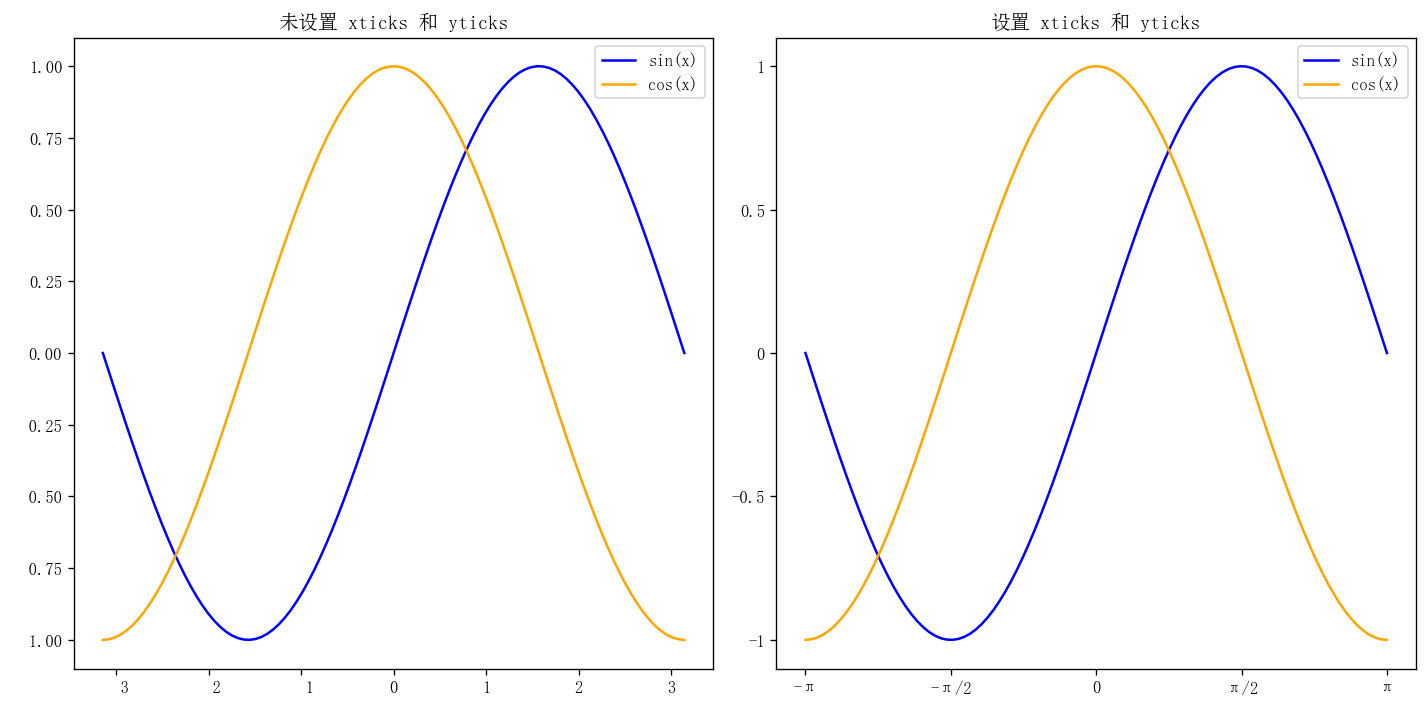
\includegraphics[width=0.6\textwidth]{part/图形化/Matplotlib/pic/图片样式与排版/ticks设置坐标.png}
    \caption{ticks设置坐标}
    \label{fig:ticks设置坐标}
\end{figure}


\subsection{坐标轴的标签}
坐标轴的标签可以通过 \codeinline{plt.xlabel()} 和 \codeinline{plt.ylabel()} 函数来设置。以下示例展示了如何设置坐标轴的标签：

\begin{lstlisting}[style=pythonstyle]
import matplotlib.pyplot as plt
import numpy as np

# 创建数据
x = np.linspace(-np.pi, np.pi, 100)
y1 = np.sin(x)
y2 = np.cos(x)

# 创建两个子图用于比较
fig, (ax1, ax2) = plt.subplots(1, 2, figsize=(12, 6))

# 第一个子图：不使用 xlabel 和 ylabel
ax1.plot(x, y1, color='blue', label='sin(x)')
ax1.plot(x, y2, color='orange', label='cos(x)')
ax1.set_xlim(-np.pi, np.pi)  # 设置 x 轴的上下限
ax1.set_ylim(-1.0, 1.0)      # 设置 y 轴的上下限
ax1.set_title('未设置 xlabel 和 ylabel')
ax1.legend()

# 第二个子图：使用 xlabel 和 ylabel
ax2.plot(x, y1, color='blue', label='sin(x)')
ax2.plot(x, y2, color='orange', label='cos(x)')
ax2.set_xlim(-np.pi, np.pi)  # 设置 x 轴的上下限
ax2.set_ylim(-1.0, 1.0)      # 设置 y 轴的上下限
ax2.set_xlabel('X 轴 (radians)')  # 设置 x 轴标签
ax2.set_ylabel('Y 轴 (value)')    # 设置 y 轴标签
ax2.set_title('设置 xlabel 和 ylabel')
ax2.legend()

# 调整布局并显示图像
plt.tight_layout()
plt.show()
\end{lstlisting}

\begin{figure}[htpb]
    \centering
    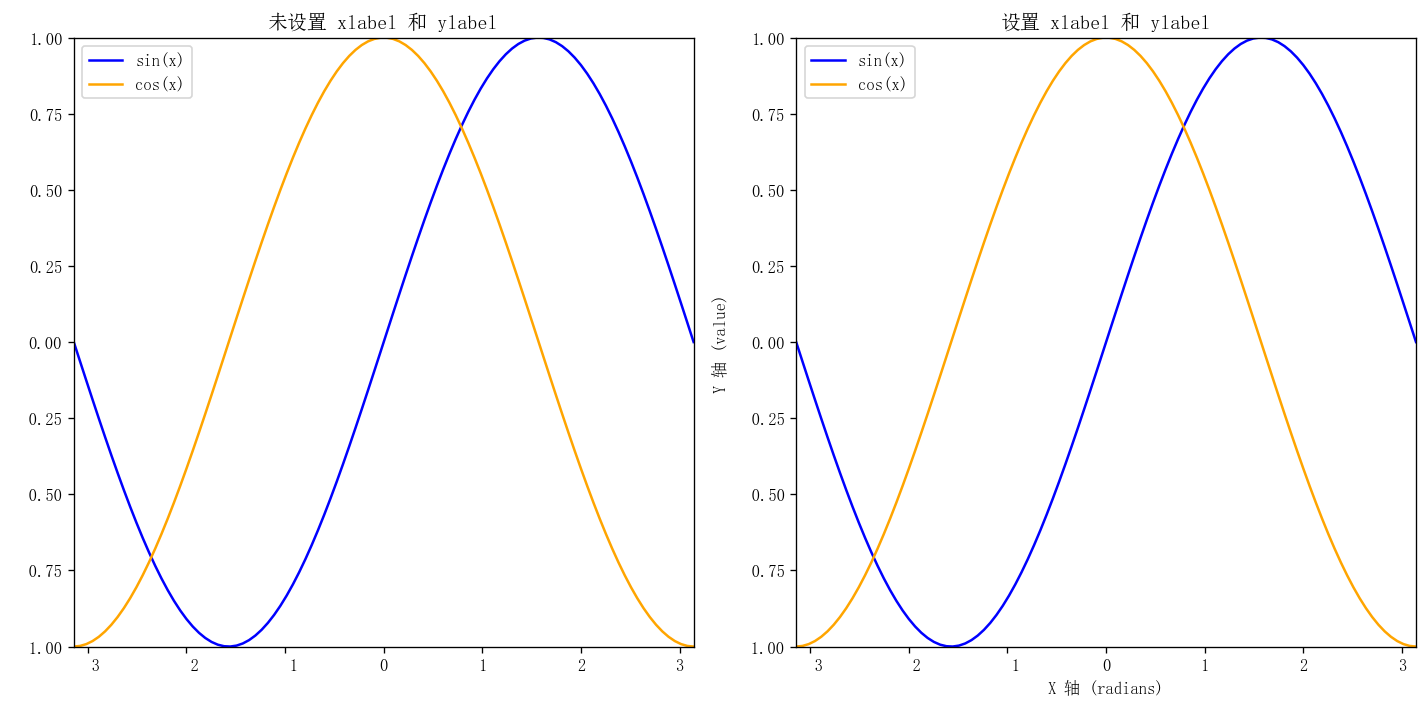
\includegraphics[width=0.6\textwidth]{part/图形化/Matplotlib/pic/图片样式与排版/label标签的设置.png}
    \caption{label标签的设置}
    \label{fig:label标签的设置}
\end{figure}

\subsection{坐标轴移动}
坐标轴线和上面的记号连在一起就形成了脊柱（Spines，一条线段上有一系列的凸起，很像脊柱骨），它记录了数据区域的范围。

默认是放到图的四边，
matplotlib 中的坐标轴线和记号线可以通过 \codeinline{spines} 属性进行设置。以下示例展示了如何将坐标轴移到图的中间：


\begin{lstlisting}[style=pythonstyle]
import matplotlib.pyplot as plt
import numpy as np

# 创建数据
x = np.linspace(-np.pi, np.pi, 100)
y1 = np.sin(x)
y2 = np.cos(x)

# 创建两个子图用于比较
fig, (ax1, ax2) = plt.subplots(1, 2, figsize=(12, 6))

# 第一个子图：默认坐标轴在图的四边
ax1.plot(x, y1, color='blue', label='sin(x)')
ax1.plot(x, y2, color='orange', label='cos(x)')
ax1.set_title('默认坐标轴位置')
ax1.legend()

# 第二个子图：将坐标轴移到图的中间
ax2.plot(x, y1, color='blue', label='sin(x)')
ax2.plot(x, y2, color='orange', label='cos(x)')
ax2.spines['top'].set_color('none')  # 隐藏上边框
ax2.spines['right'].set_color('none')  # 隐藏右边框
ax2.spines['left'].set_position(('data', 0))  # 将左侧的 y 轴移到 x = 0 位置
ax2.spines['bottom'].set_position(('data', 0))  # 将底部的 x 轴移到 y = 0 位置
ax2.set_title('坐标轴移到图的中间')
ax2.legend()

# 调整布局并显示图像
plt.tight_layout()
plt.show()
\end{lstlisting}

\begin{figure}[htpb]
    \centering
    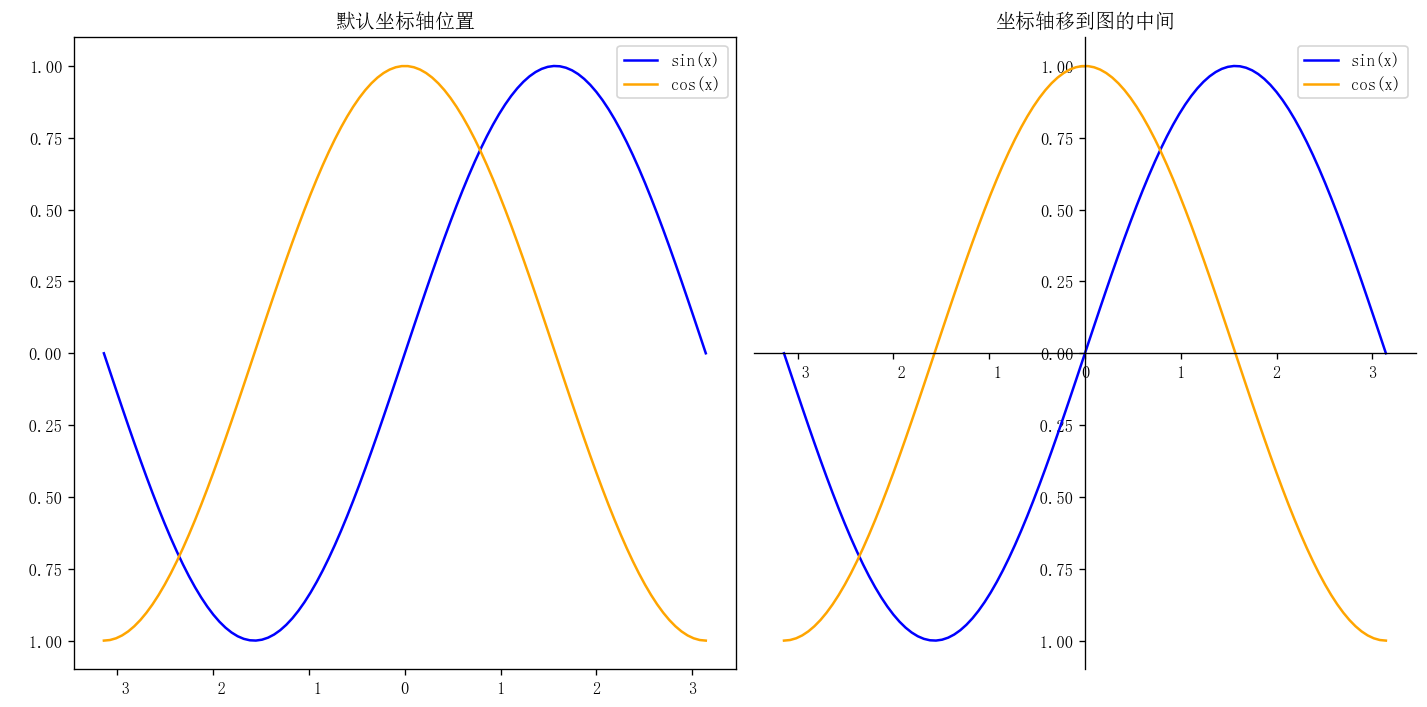
\includegraphics[width=0.6\textwidth]{part/图形化/Matplotlib/pic/图片样式与排版/spines移动坐标轴.png}
    \caption{spines移动坐标轴}
\end{figure}

\subsection{添加图例}
图例是用来区分不同数据的标签，可以通过 \codeinline{plt.legend()} 函数来添加。以下示例展示了如何添加图例：

\begin{lstlisting}[style=pythonstyle]
import matplotlib.pyplot as plt
import numpy as np

# 创建数据
x = np.linspace(-np.pi, np.pi, 100)
y1 = np.sin(x)
y2 = np.cos(x)

# 创建两个子图用于比较
fig, (ax1, ax2) = plt.subplots(1, 2, figsize=(12, 6))

# 第一个子图：不使用图例
ax1.plot(x, y1, color='orange', linewidth=1.0, linestyle='-', label='sin(x)')
ax1.plot(x, y2, color='blue', linewidth=1.0, linestyle='-', label='cos(x)')
ax1.set_title('未添加图例')
# 没有使用 ax1.legend()，因此没有图例

# 第二个子图：使用图例
ax2.plot(x, y1, color='orange', linewidth=1.0, linestyle='-', label='sin(x)')
ax2.plot(x, y2, color='blue', linewidth=1.0, linestyle='-', label='cos(x)')
ax2.set_title('添加图例')
ax2.legend(loc='upper left', fontsize='large')  # 使用图例，放在左上角，字体较大

# 调整布局并显示图像
plt.tight_layout()
plt.show()
\end{lstlisting}
\begin{figure}[htpb]
    \centering
    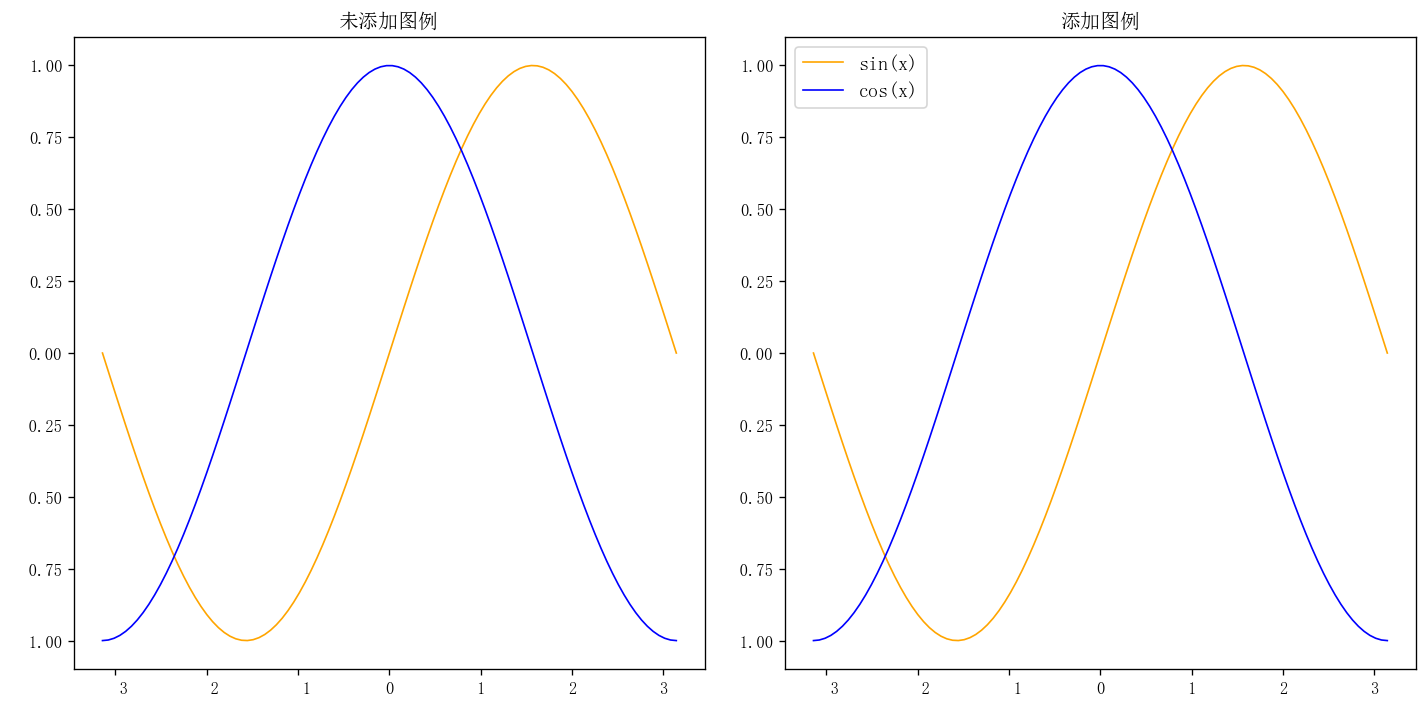
\includegraphics[width=0.6\textwidth]{part/图形化/Matplotlib/pic/图片样式与排版/legend添加图例.png}
    \caption{legend添加图例}
\end{figure}

\subsection{坐标轴的网格}
坐标轴的网格可以通过 \codeinline{plt.grid()} 函数来设置。以下示例展示了如何添加坐标轴的网格：

\begin{lstlisting}[style=pythonstyle]
import matplotlib.pyplot as plt
import numpy as np

# 创建数据
x = np.linspace(-np.pi, np.pi, 100)
y1 = np.sin(x)
y2 = np.cos(x)

# 创建两个子图用于比较
fig, (ax1, ax2) = plt.subplots(1, 2, figsize=(12, 6))

# 第一个子图：不使用网格
ax1.plot(x, y1, color='orange', linewidth=1.0, linestyle='-', label='sin(x)')
ax1.plot(x, y2, color='blue', linewidth=1.0, linestyle='-', label='cos(x)')
ax1.set_title('未使用网格')
ax1.legend(loc='upper left')

# 第二个子图：使用网格
ax2.plot(x, y1, color='orange', linewidth=1.0, linestyle='-', label='sin(x)')
ax2.plot(x, y2, color='blue', linewidth=1.0, linestyle='-', label='cos(x)')
ax2.set_title('使用网格')
ax2.legend(loc='upper left')
ax2.grid(True)  # 开启网格

# 调整布局并显示图像
plt.tight_layout()
plt.show()
\end{lstlisting}
\begin{figure}[htpb]
    \centering
    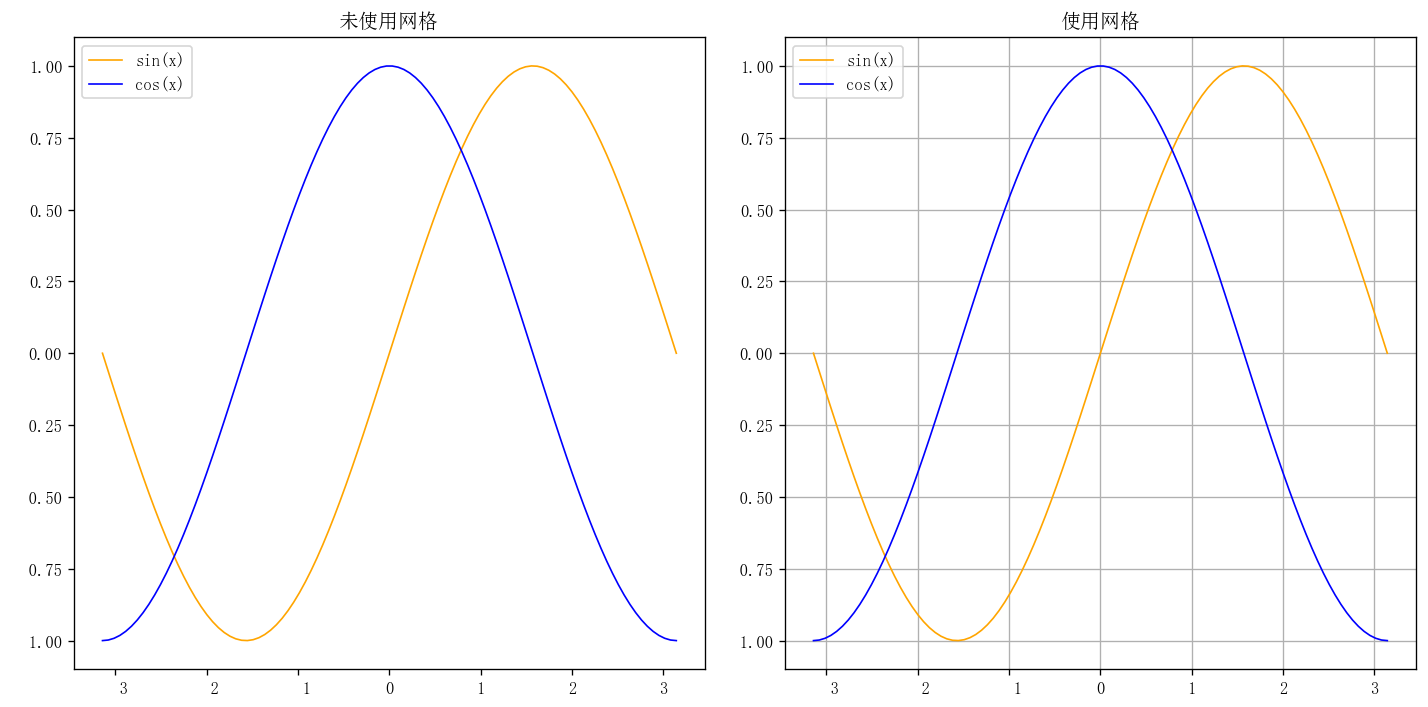
\includegraphics[width=0.6\textwidth]{part/图形化/Matplotlib/pic/图片样式与排版/grid添加网格.png}
    \caption{grid添加网格}
\end{figure}

\subsection{特殊点的注释}
特殊点的注释可以通过 \codeinline{plt.annotate()} 函数来设置。

\codeinline{plt.annotate()} 函数的主要参数包括：
\begin{enumerate}[label=\arabic*)]
    \item \codeinline{s}：注释的内容。
    \item \codeinline{xy}：注释的位置。
    \item \codeinline{xytext}：注释的文本位置。
    \item \codeinline{arrowprops}：箭头的属性。
\end{enumerate}

\begin{lstlisting}[style=pythonstyle]
import matplotlib.pyplot as plt
import numpy as np

# 创建数据
x = np.linspace(-np.pi, np.pi, 100)
y1 = np.sin(x)
y2 = np.cos(x)
t = 2 * np.pi / 3  # 特殊点的位置
t2 = -2 * np.pi / 3  # 特殊点的位置

# 创建两个子图用于比较
fig, (ax1, ax2) = plt.subplots(1, 2, figsize=(14, 6))

# 第一个子图：不添加注释
ax1.plot(x, y1, color='orange', linewidth=1.5, linestyle='-', label='sin(x)')
ax1.plot(x, y2, color='blue', linewidth=1.5, linestyle='-', label='cos(x)')
ax2.scatter([t2], [np.cos(t2)], 30, color='blue') # 添加特殊点
ax1.scatter([t], [np.sin(t)], 30, color='orange') # 添加特殊点
ax1.set_title('未添加注释')
ax1.axhline(0, color='black', linewidth=0.5) 
ax1.axvline(0, color='black', linewidth=0.5) 
ax1.legend(loc='upper left')

# 第二个子图：添加注释
ax2.plot(x, y1, color='orange', linewidth=1.5, linestyle='-', label='sin(x)')
ax2.plot(x, y2, color='blue', linewidth=1.5, linestyle='-', label='cos(x)')
ax2.scatter([t2], [np.cos(t2)], 30, color='blue')
ax2.scatter([t], [np.sin(t)], 30, color='orange')
ax2.set_title('添加注释')
ax2.axhline(0, color='black', linewidth=0.5)
ax2.axvline(0, color='black', linewidth=0.5)

# 添加注释
ax2.annotate(r'$\sin(\frac{2\pi}{3})=\frac{\sqrt{3}}{2}$',
             xy=(t, np.sin(t)), xycoords='data',
             xytext=(+10, +30), textcoords='offset points', fontsize=16,
             arrowprops=dict(arrowstyle="->", connectionstyle="arc3,rad=.2"))

ax2.annotate(r'$\cos(-\frac{2\pi}{3})=-\frac{1}{2}$',
             xy=(t2, np.cos(t2)), xycoords='data',
             xytext=(-90, 0), textcoords='offset points', fontsize=16,
             arrowprops=dict(arrowstyle="->", connectionstyle="arc3,rad=.2"))

ax2.legend(loc='upper left')

# 调整布局并显示图像
plt.tight_layout()
plt.show()
\end{lstlisting}
\begin{figure}[htpb]
    \centering
    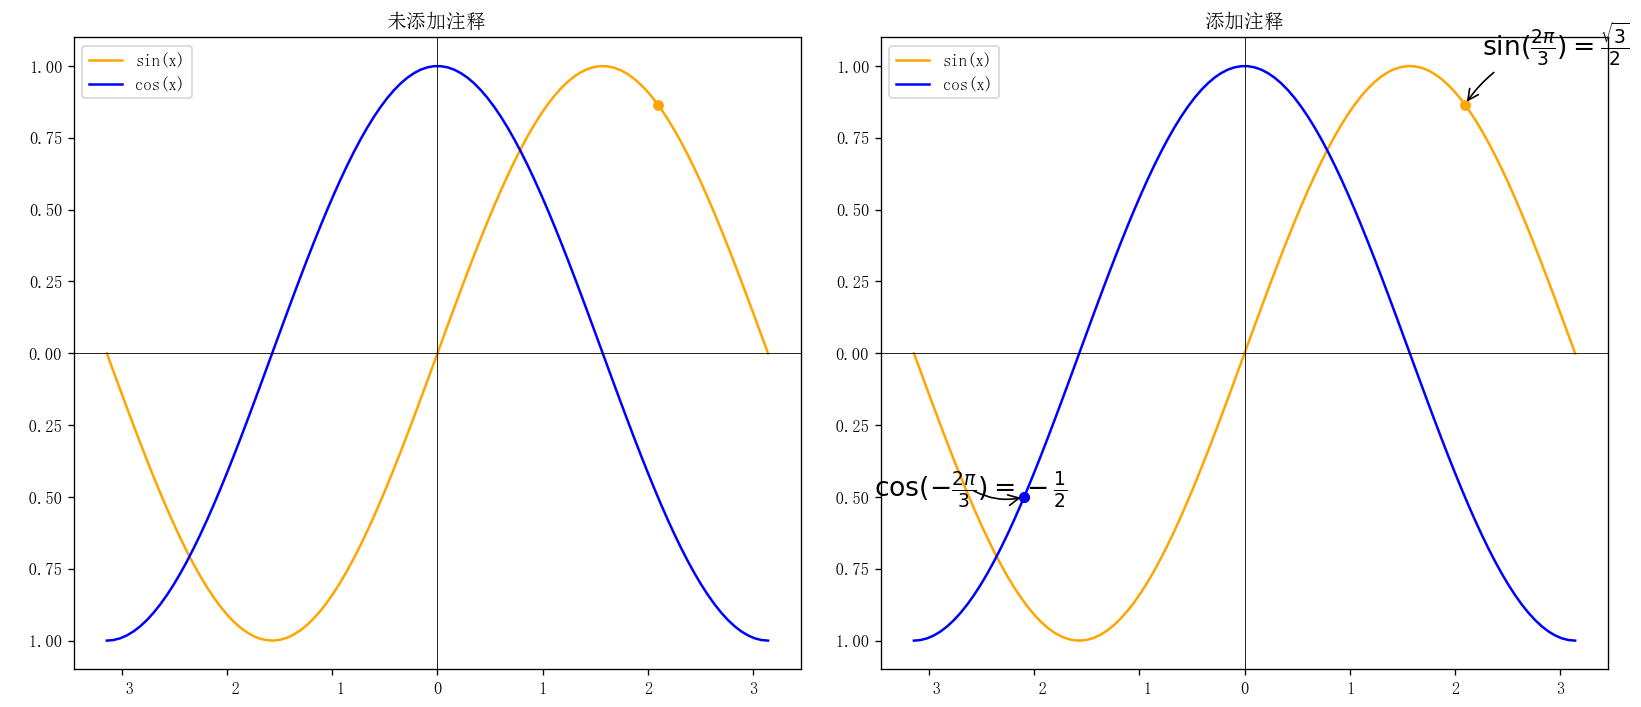
\includegraphics[width=0.6\textwidth]{part/图形化/Matplotlib/pic/图片样式与排版/annotation添加注释.png}
    \caption{annotation添加注释}
\end{figure}



\section{箭头}
箭头可以通过 \codeinline{plt.arrow()} 函数来设置。以下示例展示了如何添加箭头：

\begin{lstlisting}[style=pythonstyle]
import matplotlib.pyplot as plt

# 创建图像
plt.figure(figsize=(8, 6))

# 绘制箭头
plt.arrow(0, 0, 0.5, 0.5, width=0.02, head_width=0.1, head_length=0.1, fc='blue', ec='black')
## 从 (0, 0) 开始，到 (0.5, 0.5) 结束
## width 是箭头的宽度，head_width 是箭头的底部宽度，head_length 是箭头的长度
## fc 是箭头的填充颜色，ec 是箭头的边框颜色

plt.text(0.6, 0.6, '箭头', fontsize=12, color='black', ha='center', va='center')

# 设置坐标轴
plt.xlim(-1, 1)
plt.ylim(-1, 1)

# 添加标题
plt.title('示例：使用 plt.arrow() 添加箭头')

# 显示图像
plt.grid(True)
plt.show()
\end{lstlisting}    


\section{图片风格}
matplotlib 提供了一些预设的风格，
\begin{lstlisting}[style=demostyle, numbers=none]
print(plt.style.available[:])
>>>
['bmh', 'classic', 'dark_background', 'fivethirtyeight', 'ggplot']
\end{lstlisting}

可以通过 \codeinline{plt.style.use()} 函数来设置。以下示例展示了如何设置图片风格：

\begin{lstlisting}[style=pythonstyle]
import matplotlib.pyplot as plt
import numpy as np

# 数据生成
x = np.linspace(0, 10, 100)
y1 = np.sin(x)
y2 = np.cos(x)

# 定义绘图风格
styles = ['Solarize_Light2', '_classic_test_patch', '_mpl-gallery', '_mpl-gallery-nogrid', 
          'bmh', 'classic', 'dark_background', 'fast', 'fivethirtyeight', 'ggplot', 
          'grayscale', 'seaborn-v0_8', 'seaborn-v0_8-bright', 'seaborn-v0_8-colorblind', 
          'seaborn-v0_8-dark', 'seaborn-v0_8-dark-palette', 'seaborn-v0_8-darkgrid', 
          'seaborn-v0_8-deep', 'seaborn-v0_8-muted', 'seaborn-v0_8-notebook', 
          'seaborn-v0_8-paper', 'seaborn-v0_8-pastel', 'seaborn-v0_8-poster', 
          'seaborn-v0_8-talk', 'seaborn-v0_8-ticks', 'seaborn-v0_8-white', 
          'seaborn-v0_8-whitegrid', 'tableau-colorblind10']

# 计算行数和列数，每行3个
n_cols = 3
n_rows = (len(styles) + n_cols - 1) // n_cols  # 计算需要的行数

# 创建图和子图
fig, axs = plt.subplots(n_rows, n_cols, figsize=(10, n_rows * 3))
axs = axs.flatten()  # 展平成一维数组便于遍历

# 绘制每种风格
for i, style in enumerate(styles):
    plt.style.use(style)  # 设置当前风格
    axs[i].plot(x, y1, label='sin(x)')
    axs[i].plot(x, y2, label='cos(x)')
    axs[i].set_title(f'Style: {style}', fontsize=10)
    axs[i].legend(loc='upper right', fontsize=8)
    axs[i].grid(True)

# 隐藏多余的子图
for j in range(len(styles), len(axs)):
    axs[j].axis('off')

# 调整布局
plt.tight_layout()
plt.show()
\end{lstlisting}    
\begin{figure}[htpb]
    \centering
    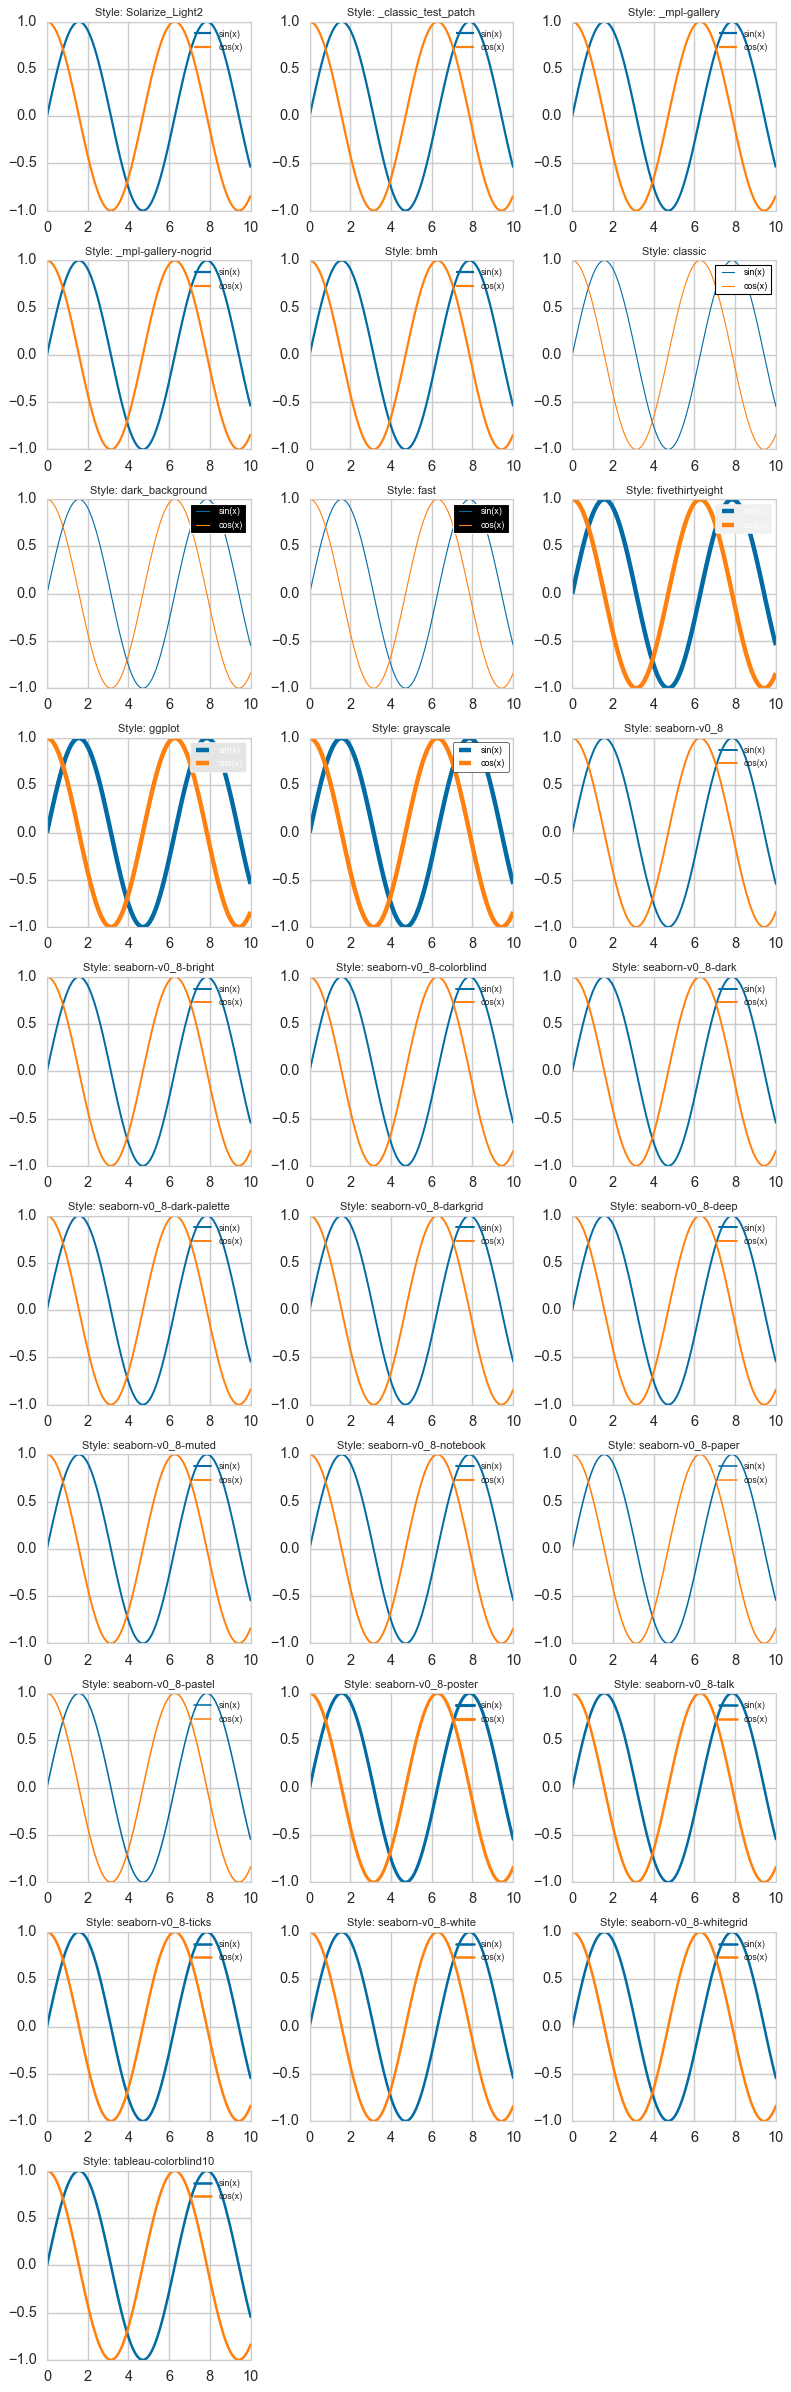
\includegraphics[width=0.6\textwidth]{part/图形化/Matplotlib/pic/图片样式与排版/style设置绘图风格.png}
    \caption{style设置绘图风格}
\end{figure}


\section{多图的排列}
Matplotlib 提供了多种方法来绘制子图，常用的方法包括 
\codeinline{plt.subplot()}、\codeinline{plt.subplots()} 和 \codeinline{GridSpec}。

\subsection{plt.subplot()}
\codeinline{plt.subplot()} 可以快速创建子图。
\begin{lstlisting}[style=demostyle, numbers=none]
plt.subplot(nrows, ncols, index)
# nrows：子图的行数
# ncols：子图的列数
# index：子图的索引，从1开始
\end{lstlisting}

\begin{lstlisting}[style=pythonstyle]
import matplotlib.pyplot as plt
import numpy as np

# 创建数据
x = np.linspace(0, 10, 100)
y1 = np.sin(x)
y2 = np.cos(x)

# 创建一个2行1列的子图布局，绘制第一个子图
plt.subplot(2, 1, 1) # 创建一个2行1列的布局，子图在第1个位置
plt.plot(x, y1)
plt.title('Sine Function')

# 创建一个2行1列的子图布局，绘制第二个子图
plt.subplot(2, 1, 2)
plt.plot(x, y2)
plt.title('Cosine Function')

# 显示图像
plt.tight_layout()  # 自动调整子图间距
plt.show()
\end{lstlisting}
\begin{figure}[htpb]
    \centering
    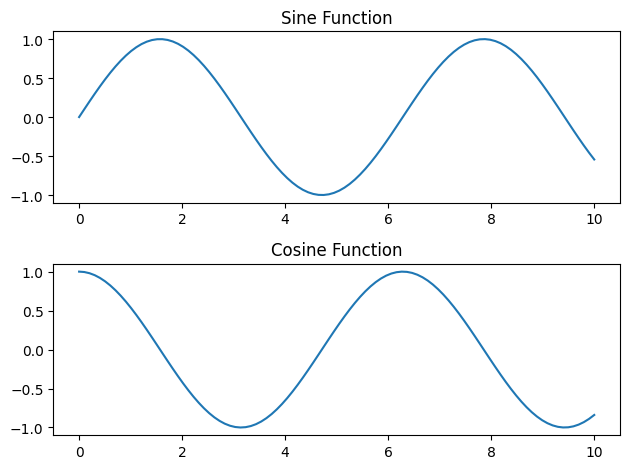
\includegraphics[width=0.4\textwidth]{part/图形化/Matplotlib/pic/图片样式与排版/plt.subplot创建子图演示.png}
    \caption{plt.subplot()创建子图演示}
\end{figure}

\subsubsection{add\_subplot()添加子图}
\codeinline{plt.subplot()} 函数返回的是当前子图对象，可以通过 \codeinline{add\_subplot()} 方法来添加子图。
\begin{lstlisting}[style=demostyle, numbers=none]
ax = fig.add_subplot(nrows, ncols, index)
# nrows：子图的行数
# ncols：子图的列数
# index：子图的索引，从1开始
\end{lstlisting}

\begin{lstlisting}[style=pythonstyle]
import numpy as np
import matplotlib.pyplot as plt

# 创建数据
rad = np.arange(0, np.pi * 2, 0.01)

# 创建图形对象 p1
p1 = plt.figure(figsize=(8, 10), dpi=80)  # 确定画布大小

# 第一个子图
ax1 = p1.add_subplot(2, 1, 1)  # 创建一个两行1列的子图，并开始绘制第一幅
plt.title('lines')  # 添加标题
plt.xlabel('x1')  # 添加x轴的名称
plt.ylabel('y1')  # 添加y轴的名称
plt.xlim((0, 1))  # 确定x轴范围
plt.ylim((0, 1))  # 确定y轴范围
plt.xticks([0, 0.2, 0.4, 0.6, 0.8, 1])  # 规定x轴刻度
plt.yticks([0, 0.2, 0.4, 0.6, 0.8, 1])  # 确定y轴刻度
plt.plot(rad, rad)  # 添加 y = x 曲线
plt.plot(rad, rad**2)  # 添加 y = x^2 曲线
plt.legend(['y=x', 'y=x^2'])

# 第二个子图
ax2 = p1.add_subplot(2, 1, 2)  # 开始绘制第2幅
plt.title('sin/cos')  # 添加标题
plt.xlabel('x2')  # 添加x轴的名称
plt.ylabel('y2')  # 添加y轴的名称
plt.xlim((0, np.pi * 2))  # 确定x轴范围
plt.ylim((-1, 1))  # 确定y轴范围
plt.xticks([0, np.pi / 2, np.pi, np.pi * 1.5, np.pi * 2])  # 规定x轴刻度
plt.yticks([-1, -0.5, 0, 0.5, 1])  # 确定y轴刻度
plt.plot(rad, np.sin(rad))  # 添加 sin 曲线
plt.plot(rad, np.cos(rad))  # 添加 cos 曲线
plt.legend(['sin', 'cos'])

# 保存并显示图像
plt.savefig('../tmp/subplot通过add_subplot添加子图.png')
plt.show()
\end{lstlisting}

\begin{figure}[htpb]
    \centering
    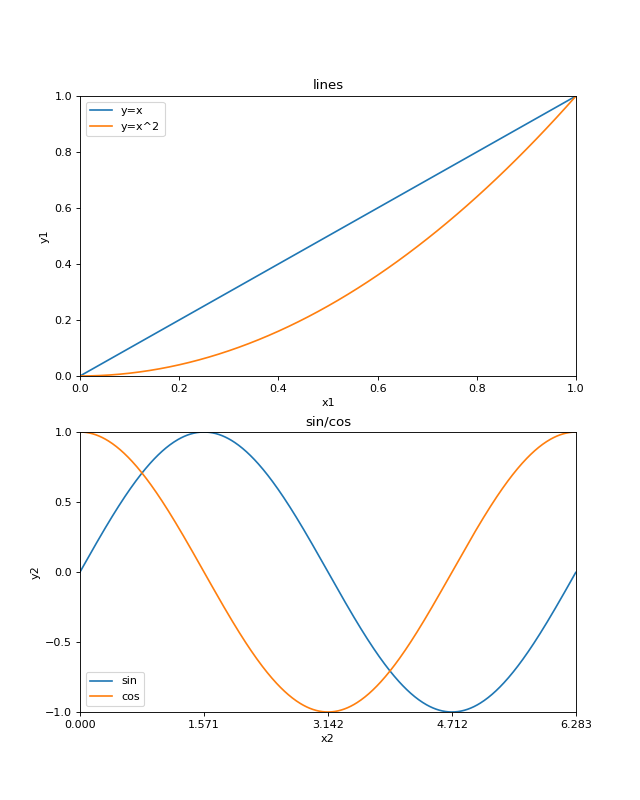
\includegraphics[width=0.4\textwidth]{part/图形化/Matplotlib/pic/图片样式与排版/subplot通过add_subplot添加子图.png}
    \caption{subplot通过add\_subplot添加子图}
\end{figure}




\subsection{plt.subplots()}
\codeinline{plt.subplots()} 是 Matplotlib 中创建子图的推荐方法，它返回一个图形对象和一个包含所有子图的数组对象。
\begin{lstlisting}[style=demostyle, numbers=none]
fig, axs = plt.subplots(nrows, ncols)
# nrows：子图的行数
# ncols：子图的列数
\end{lstlisting}

\begin{lstlisting}[style=pythonstyle]
import matplotlib.pyplot as plt
import numpy as np

# 创建数据
x = np.linspace(0, 10, 100)
y1 = np.sin(x)
y2 = np.cos(x)

# 使用 subplots 创建 1行2列的子图布局
fig, axs = plt.subplots(1, 2, figsize=(10, 4))

# 绘制第一个子图
axs[0].plot(x, y1, 'r-')
axs[0].set_title('Sine Function')

# 绘制第二个子图
axs[1].plot(x, y2, 'b-')
axs[1].set_title('Cosine Function')

# 调整子图布局
plt.tight_layout()
plt.show()
\end{lstlisting}
\begin{figure}[htpb]
    \centering
    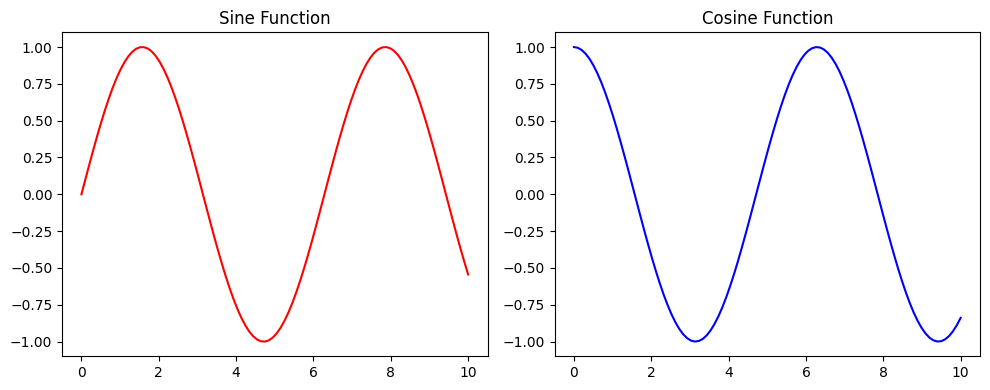
\includegraphics[width=0.4\textwidth]{part/图形化/Matplotlib/pic/图片样式与排版/plt.subplots创建子图演示.png}
    \caption{plt.subplots()创建子图演示}
\end{figure}


\subsection{GridSpec}
\codeinline{GridSpec} 提供了更灵活的方式来创建复杂的子图布局。
通过 \codeinline{GridSpec} 可以更细致地控制子图的大小和位置。
\begin{lstlisting}[style=demostyle, numbers=none]
from matplotlib.gridspec import GridSpec
gs = GridSpec(nrows, ncols)
# nrows：子图的行数
# ncols：子图的列数

ax = fig.add_subplot(gs[row, col])
# gs[row, col]：获取第 row 行第 col 列的子图
# row：子图的行索引，从0开始
# col：子图的列索引，从0开始
\end{lstlisting}

\begin{lstlisting}[style=pythonstyle]
import matplotlib.pyplot as plt
import numpy as np
from matplotlib.gridspec import GridSpec

# 创建数据
x = np.linspace(0, 10, 100)
y1 = np.sin(x)
y2 = np.cos(x)
y3 = np.tan(x)

# 创建一个新的图形
fig = plt.figure(figsize=(8, 6))

# 创建一个2x2的网格布局
gs = GridSpec(2, 2, figure=fig)

# 绘制子图1，占据第1行的全部
ax1 = fig.add_subplot(gs[0, :])
ax1.plot(x, y1, 'g-')
ax1.set_title('Sine Function')

# 绘制子图2，占据第2行第1列
ax2 = fig.add_subplot(gs[1, 0])
ax2.plot(x, y2, 'r-')
ax2.set_title('Cosine Function')

# 绘制子图3，占据第2行第2列
ax3 = fig.add_subplot(gs[1, 1])
ax3.plot(x, y3, 'b-')
ax3.set_title('Tangent Function')

# 调整子图布局
plt.tight_layout()
plt.show()
\end{lstlisting}
\begin{figure}[htpb]
    \centering
    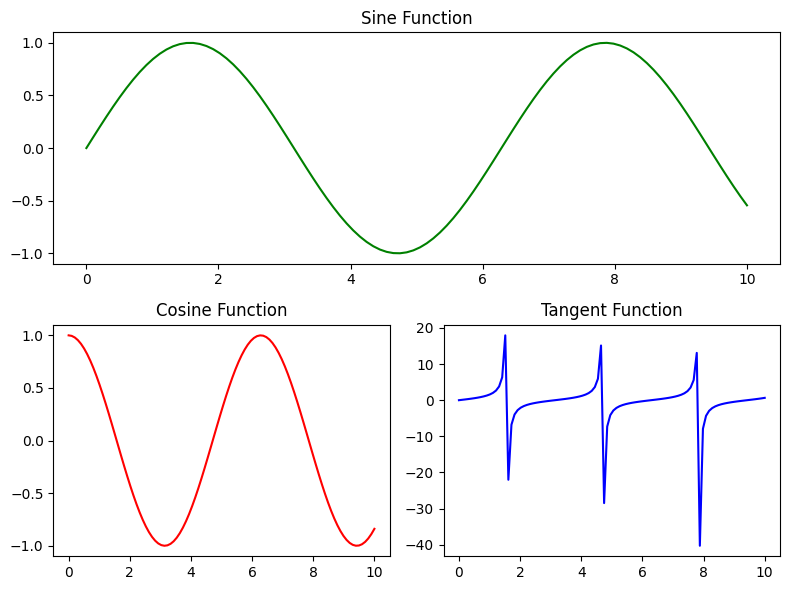
\includegraphics[width=0.4\textwidth]{part/图形化/Matplotlib/pic/图片样式与排版/GridSpec创建子图演示.png}
    \caption{GridSpec创建子图演示}
\end{figure}


\subsection{自定义子图大小和间距}
使用 \codeinline{plt.subplots\_adjust()} 可以调整子图之间的间距，方便对布局进行微调。
\begin{lstlisting}[style=demostyle, numbers=none]
plt.subplots_adjust(left=None, bottom=None, right=None, top=None, wspace=None, hspace=None)
# left：左边距比例，默认为0.125
# bottom：下边距比例，默认为0.11
# right：右边距比例，默认为0.9
# top：上边距比例，默认为0.88
# wspace：水平间距比例，默认为0.2
# hspace：垂直间距比例，默认为0.2
\end{lstlisting}

\begin{lstlisting}[style=pythonstyle]
import matplotlib.pyplot as plt
import numpy as np

# 创建数据
x = np.linspace(0, 10, 100)
y1 = np.sin(x)
y2 = np.cos(x)

# 创建一个2x1的子图
fig, (ax1, ax2) = plt.subplots(2, 1, figsize=(8, 6))

# 绘制子图
ax1.plot(x, y1, 'm-')
ax1.set_title('Sine Function')

ax2.plot(x, y2, 'c-')
ax2.set_title('Cosine Function')

# 调整子图之间的间距
plt.subplots_adjust(hspace=0.4, wspace=0.3)
plt.show()
\end{lstlisting}



%% Pyecharts
\chapter{[Python库] Pyecharts概述}
\label{cha:pyecharts_intro}
\section{简介}
\label{sec:pyecharts_intro}
\href{https://pyecharts.org/#/zh-cn/}{Echarts} 是一个由百度开源的数据可视化，凭借着良好的交互性，精巧的图表设计，得到了众多开发者的认可。
而 Python 是一门富有表达力的语言，很适合用于数据处理。

\begin{enumerate}[itemindent=1em,label=\arabic*)]
    \item V0.5x版本：不在维护，支持 Python2.7，3.4+
    \item V1.0版本：v0.5.X 和 v1 间不兼容，\textcolor{red}{\textbf{仅}}支持python3.6及以上版本
    \item V2.0版本：支持 Python3.6 ~ Python 3.11
\end{enumerate}

\section{安装}
\label{sec:pyecharts_install}
\begin{lstlisting}[style=demostyle,numbers=none]
pip install pyecharts

# 检查版本
$ python
Python 3.10.14 (main, May  6 2024, 19:42:50) [GCC 11.2.0] on linux
Type "help", "copyright", "credits" or "license" for more information.
>>> import pyecharts
s.__version__)>>>
>>> print(pyecharts.__version__)
2.0.6
\end{lstlisting}

源码安装
\begin{lstlisting}[style=demostyle,numbers=none]
$ git clone https://github.com/pyecharts/pyecharts.git
$ cd pyecharts
$ pip install -r requirements.txt -i https://pypi.tuna.tsinghua.edu.cn/simple
$ python setup.py install
# 或者执行 python install.py
\end{lstlisting}




\chapter{图表类型}
%% manim
\chapter{Manim概述}
\section{简介}
Manim 最初由 Grant Sanderson 创建，用于他的 YouTube 频道 3Blue1Brown。随着频道的受欢迎程度增加，许多人想使用 Manim 来制作自己的项目。然而，最初的 Manim 仅供个人使用，其他用户很难安装和使用。

\begin{enumerate}[label=\arabic*)]
    \item 2019 年底: Grant 开始在一个新分支（Shaders 分支）上工作，以实现更快的 OpenGL 渲染。
    \item 2020 年中: 一组开发者将其分叉成现在的社区版（\href{https://github.com/ManimCommunity/manim/}{ManimCE}）。
    \item 2021 年初: Grant 将 Shaders 分支合并回主分支，形成了 ManimGL。
\end{enumerate}


        
\section{Manim(ManimCE)}
\begin{enumerate}[label=\arabic*)]
    \item Manim官网: \url{https://www.manim.community/}
    \item Manim项目地址: \url{https://github.com/ManimCommunity/manim#command-line-arguments}
    \item Manim 文档: \url{https://docs.manim.community/en/stable/#}
    % https://mp.weixin.qq.com/mp/appmsgalbum?__biz=MzkyODIzMDczMQ==&action=getalbum&album_id=2793721415848935425&scene=173&subscene=&sessionid=svr_d8d296e7dbe&enterid=1726627760&from_msgid=2247483712&from_itemidx=1&count=3&nolastread=1#wechat_redirect
    % https://mp.weixin.qq.com/mp/appmsgalbum?__biz=MzIxNDc3NDc3NQ==&action=getalbum&album_id=3434147620531159045&scene=173&subscene=&sessionid=undefined&enterid=0&from_msgid=2247484898&from_itemidx=1&count=3&nolastread=1#wechat_redirect
\end{enumerate}

PyPi包名：\codeinline{manim}

\subsection{安装}
\begin{lstlisting}[style=demostyle,numbers=none]
pip install manim
pip install manim  -i https://mirrors.aliyun.com/pypi/simple/
\end{lstlisting}

\begin{lstlisting}[style=demostyle,numbers=none]
conda create -n my-manim-environment
conda activate my-manim-environment    
conda install -c conda-forge manim
\end{lstlisting}

\subsection{使用}
\begin{lstlisting}[style=demostyle,numbers=none]
manim [options] <filename> <scene_name>
# 1.<filename>: 指定包含动画场景的Python脚本文件名（如myfile.py）
# 2.<scene_name>: 指定要渲染的场景名称(可选，如果不指定，Manim会渲染文件中的第一个场景)
# 3.<options>: 可选参数
-h, --help: 显示帮助信息，列出所有可用的参数。
-p, --preview: 渲染完成后自动播放动画。
-ql, --quality low: 以低质量（快速预览模式）渲染动画，适用于快速测试（15fps, 480p）。
-qm, --quality medium: 以中等质量渲染动画（30fps, 720p）。
-qh, --quality high: 以高质量渲染动画（60fps, 1080p）。
-qk, --quality 4k: 以4K超高清质量渲染动画（60fps, 2160p）。
-s, --save_last_frame: 只渲染场景的最后一帧并保存为图像文件。
-i, --save_as_gif: 将渲染的场景保存为GIF文件。
--renderer [cairo | opengl]: 指定使用哪种渲染器（默认为cairo，opengl为高性能渲染器）。
-r, --resolution <height>x<width>: 设置输出视频的分辨率。例如-r 1920x1080为1080p高清分辨率。
    -r 854,480:生成 480p 分辨率的视频
    -r 1280,720:生成 720p 分辨率的视频
    -r 1920,1080:生成 1080p 分辨率的视频
    -r 2560,1440:生成 1440p 分辨率的视频
    -r 3840,2160:生成 2160p 分辨率的视频
--fps <number>: 设置视频帧率（每秒帧数）。
-o, --output_file <path>: 指定输出文件的路径和文件名。
--config_file <path>: 指定自定义配置文件路径，用于设置渲染器的配置。
--progress_bar: 显示渲染进度条。
--log_level [DEBUG | INFO | WARNING | ERROR | CRITICAL]: 设置日志级别，控制输出信息的详细程度。
--write_to_movie: 强制将场景输出为视频文件（mp4格式）

# 最常用的是 -pql 参数，用于快速预览
manim -ql -p myfile.py MyScene
\end{lstlisting}    

\subsection{测试}
\begin{lstlisting}[style=pythonstyle]
# 测试中文能否显示
# manim -p .\sample.py 
# -*- coding: utf-8 -*-
from manim import *

class TransformExample(Scene):
    def construct(self):
        banner = ManimBanner()
        banner.shift(UP * 0.5)
        self.play(banner.create(), run_time=1)
        self.play(banner.animate.scale(0.3), run_time=0.5)
        self.play(banner.expand(), run_time=1)

        t = Text("测试中文能否显示").next_to(banner, DOWN * 2)
        tex = VGroup(
            Text("测试数学公式:", font_size=30),
            Tex(r"$\sum_{n=1}^\infty \frac{1}{n^2} = \frac{\pi^2}{6}$"),
        )
        tex.arrange(RIGHT, buff=SMALL_BUFF)
        tex.next_to(t, DOWN)
        self.play(Write(t), run_time=1)
        self.play(Write(tex), run_time=1)

        self.wait()
\end{lstlisting}

\section{ManimGL}
由 Grant Sanderson 维护的最新版本，具有更多实验性功能，PyPI 包名为 \codeinline{manimgl}。

\url{https://3b1b.github.io/manim/getting_started/installation.html#}

\section{ManimCairo}
Manim 的 Cairo 渲染器，OpenGL 渲染前的旧版本，仅用于渲染 Grant 的旧视频，PyPI 包名为 \codeinline{manimlib}。

\chapter{Manim基本图形}
\section{点}
点是最简单图形，也是其他所有图形的基础。 绘制其他任何图形时，都是用点来定位的。

\begin{lstlisting}[style=demostyle,numbers=none]
Dot([x, y, z])
Dot([x, y, z], color=color)
\end{lstlisting}    

\begin{lstlisting}[style=pythonstyle]
# manim -pql 01Dot_demo.py DotSample    
from manim import *
class DotSample(Scene):
    def construct(self):
        # 绘制 9个点
        for x in range(-1, 2):
            for y in range(1, -2, -1):
                p = Dot([x, y, 0], color=PURPLE)
                self.play(Create(p), run_time=0.5)
\end{lstlisting}                

\section{线}
\subsection{直线}
提供任意2个点，manim通过 \codeinline{Line} 来绘制线。
\begin{lstlisting}[style=demostyle,numbers=none]
Line(start=[x1, y1, z1], end=[x2, y2, z2])
Line(start=[x1, y1, z1], end=[x2, y2, z2], color=color)
\end{lstlisting}
\begin{lstlisting}[style=pythonstyle]
# manim -pql 01Line_demo.py LineSample    
from manim import *
class LineSample(Scene):
    def construct(self):
        # 绘制 9个点
        count = 0
        for x in range(-1, 2):
            for y in range(1, -2, -1):
                p1 = Dot([x, y, 0], color=PURPLE)
                p2 = Dot([x+1, y+1, 0], color=PURPLE)
                l = Line(p1.get_center(), p2.get_center(), color=BLUE)
                self.play(Create(p1), Create(p2), Create(l), run_time=0.5+count)
                count += 0.5
\end{lstlisting}    

\subsection{虚线}
提供任意2个点，manim通过 \codeinline{DashedLine} 来绘制虚线。
\begin{lstlisting}[style=demostyle,numbers=none]
DashedLine(start=[x1, y1, z1], end=[x2, y2, z2])
DashedLine(start=[x1, y1, z1], end=[x2, y2, z2], color=color)
\end{lstlisting}

\begin{lstlisting}[style=pythonstyle]
# manim -pql 01DashedLine_demo.py DashedLineSample    
from manim import *
class DashedLineSample(Scene):
    def construct(self):
        self._dashedLines()
        self.wait()

    def _dashedLines(self):
        dl = DashedLine([-1, 1, 0], [1, 1, 0])
        self.play(Create(dl), run_time=0.5)

        dl = DashedLine([-1, 0, 0], [1, 0, 0])
        self.play(Create(dl), run_time=0.5)

        dl = DashedLine([-1, -1, 0], [1, -1, 0])
        self.play(Create(dl), run_time=0.5)
\end{lstlisting}

\subsection{带箭头的线}
提供任意2个点，manim通过 \codeinline{Arrow} 来绘制带箭头的线。
\begin{lstlisting}[style=demostyle,numbers=none]
Arrow(start=[x1, y1, z1], end=[x2, y2, z2])
Arrow(start=[x1, y1, z1], end=[x2, y2, z2], color=color)
\end{lstlisting}

\begin{lstlisting}[style=pythonstyle]
# manim -pql 01Arrow_demo.py ArrowSample    
from manim import *
class ArrowSample(Scene):
    def construct(self):
        self._arrows()  

    def _arrows(self):
        a = Arrow([-1, 1, 0], [1, 1, 0])  
        self.play(Create(a), run_time=0.5)

        a = Arrow([-1, 0, 0], [1, 0, 0])  
        self.play(Create(a), run_time=0.5)

        a = Arrow([-1, -1, 0], [1, -1, 0])  
        self.play(Create(a), run_time=0.5)
\end{lstlisting}


\section{圆}
\subsection{正圆}
绘制圆只要提供半径即可，圆心默认在屏幕的中心。 绘制圆使用 \codeinline{Circle}。
\begin{lstlisting}[style=demostyle,numbers=none]
Circle(radius=r)
Circle(radius=r, color=color)

# 通过指定圆心
Circle(radius=r, arc_center=[x, y, z])
\end{lstlisting}

\begin{lstlisting}[style=pythonstyle]
# manim -pql 01Circle_demo.py CircleSample    
from manim import *
class CircleSample(Scene):
    def construct(self):
        self._circles()

    def _circles(self):
        c = Circle(radius=1)
        self.play(Create(c), run_time=0.5)

        c = Circle(radius=1, color=PURPLE, arc_center=[-2, 3, 0])
        self.play(Create(c), run_time=0.5)
\end{lstlisting}

\subsection{椭圆}
绘制椭圆只要提供长轴和短轴即可，圆心默认在屏幕的中心。 绘制椭圆使用 \codeinline{Ellipse}。
\begin{lstlisting}[style=demostyle,numbers=none]
# width和 height分别控制椭圆最大宽度和最大高度
Ellipse(width=w, height=h)
Ellipse(width=w, height=h, color=color)

# 通过指定圆心
Ellipse(width=w, height=h, arc_center=[x, y, z])
\end{lstlisting}

\begin{lstlisting}[style=pythonstyle]
# manim -pql 01Ellipse_demo.py EllipseSample    
from manim import *
class EllipseSample(Scene):
    def construct(self):
        self._ellipses()

    def _ellipses(self):
        e = Ellipse(width=2, height=1)
        self.play(Create(e), run_time=0.5)

        e = Ellipse(width=3, height=1.5, color=PURPLE, arc_center=[-2, 3, 0])
        self.play(Create(e), run_time=0.5)
\end{lstlisting}

\subsection{圆弧}
绘制圆弧只要提供半径和角度即可，圆心默认在屏幕的中心。 绘制圆弧使用 \codeinline{Arc}。
\begin{lstlisting}[style=demostyle,numbers=none]
# 1. angle：圆弧的弧度
# 2. start_angle: 开始的角度，默认 0
# 3. radius：圆弧的半径    
Arc(radius=r, angle=angle)
Arc(radius=r, angle=angle, color=color)

# 通过指定圆心
Arc(radius=r, angle=angle, start_angle=start_angle, arc_center=[x, y, z])
\end{lstlisting}
\begin{lstlisting}[style=pythonstyle]
# manim -pql 01Arc_demo.py ArcSample    
from manim import *
class ArcSample(Scene):
    def construct(self):
        self._arcs()

    def _arcs(self):
        # 90度的圆弧, 默认圆心在屏幕中心, 半径为1
        a = Arc(radius=1, angle=PI/2)
        self.play(Create(a), run_time=0.5)

        # 180度圆弧，半径2
        a = Arc(angle=PI, radius=2, color=BLUE)
        self.play(Create(a), run_time=0.5)

        # 30度圆弧，半径2，从270度开始绘制
        a = Arc(angle=PI / 6, start_angle=PI * 1.5, radius=2, color=RED)
        self.play(Create(a), run_time=0.5)

        # 90度圆弧，半径1，圆心在[-2, 3, 0]
        a = Arc(radius=1, angle=PI/2, color=PURPLE, arc_center=[-2, 3, 0])
        self.play(Create(a), run_time=0.5)
\end{lstlisting}

\section{多边形}
\subsection{三角形}
绘制等边三角形只要提供边长即可，圆心默认在屏幕的中心。绘制等边三角形使用 \codeinline{Triangle}。

\begin{lstlisting}[style=pythonstyle]
# 创建等边三角形
# manim -pql 01Triangle_demo.py TriangleSample
from manim import *    
class PolygonSample(Scene):
    def construct(self):
        self._triangles()
        self.wait()

    def _triangles(self):
        t = Triangle()
        self.play(Create(t))
\end{lstlisting}

\begin{lstlisting}[style=demostyle,numbers=none]
Triangle(**kwargs)
# 1.vertices:
    类型: 列表或元组
    描述: 定义三角形的三个顶点。通常以 (x1, y1), (x2, y2), (x3, y3) 的形式传递，表示三角形的三个角的坐标。

# 2.fill_color:
    类型: 字符串（颜色名称或十六进制颜色代码）
    描述: 指定三角形的填充颜色。例如，可以使用 'red'、'blue' 或 '#FF5733' 等。

# 3.border_color:
    类型: 字符串（颜色名称或十六进制颜色代码）
    描述: 指定三角形边框的颜色。

# 4.border_width:
    类型: 浮点数或整数
    描述: 设置三角形边框的宽度，以像素为单位。

# 5.opacity:
    类型: 浮点数，通常在 0 到 1 之间
    描述: 设置三角形的透明度，0 表示完全透明，1 表示完全不透明。

# 6.position:
    类型: 列表或元组
    描述: 指定三角形的绘制位置，可能以 (x, y) 的形式传递，表示三角形的起始点。

# 7.rotation:
    类型: 浮点数
    描述: 指定三角形的旋转角度，以弧度或度为单位。
\end{lstlisting}

\begin{lstlisting}[style=pythonstyle]
# manim -pql 01Triangle_demo.py TriangleSample    
from manim import *

class TriangleSample(Scene):
    def construct(self):
        self._triangles()

    def _triangles(self):
        # 1.创建简单的三角形
        t = Triangle()
        self.play(Create(t))
        self.wait(2)

        # 清空画布
        self.play(Uncreate(t))
\end{lstlisting}

\subsection{矩形}
\subsubsection{正方形}
绘制正方形只要提供边长即可，圆心默认在屏幕的中心。绘制正方形使用 \codeinline{Square}。

\begin{lstlisting}[style=demostyle,numbers=none]
Square(side_length=l)
Square(side_length=l, color=color)

\end{lstlisting}    

\begin{lstlisting}[style=pythonstyle]
# manim -pql 01Square_demo.py SquareSample
from manim import *

class SquareSample(Scene):
    def construct(self):
        self._squares()

    def _squares(self):
        # 1.创建简单的正方形
        s1 = Square(side_length=1)
        self.play(Create(s1))
        
        s2 = Square(side_length=1.5)
        self.play(Create(s2), run_time=0.5)

        s3 = Square() # 默认边长为2
        self.play(Create(s3), run_time=0.5)
        self.wait(2)
        self.play(Uncreate(s3))
        self.play(Uncreate(s2))
        self.play(Uncreate(s1))

        # 2.自定义正方形
        s = Square(side_length=5, color=BLUE)
        s.move_to([-2, 3, 0])
        s.rotate(PI/4)
        self.play(Create(s), run_time=2)
        self.wait(2)
\end{lstlisting}

\subsubsection{矩形}
绘制矩形只要提供宽度和高度即可，圆心默认在屏幕的中心。绘制矩形使用 \codeinline{Rectangle}。

\begin{lstlisting}[style=demostyle,numbers=none]
Rectangle(width=w, height=h)
Rectangle(width=w, height=h, color=color)
\end{lstlisting}

\begin{lstlisting}[style=pythonstyle]
# manim -pql 01Rectangle_demo.py RectangleSample
from manim import *

class RectangleSample(Scene):
    def construct(self):
        self._rectangles()

    def _rectangles(self):
        # 1.创建简单的矩形
        r1 = Rectangle(width=2, height=1)
        self.play(Create(r1))
        
        r2 = Rectangle(width=2.5, height=1.5)
        self.play(Create(r2), run_time=0.5)

        r3 = Rectangle() # 默认宽度为4，高度为2
        self.play(Create(r3), run_time=0.5)
        self.wait(2)
        self.play(Uncreate(r3))
        self.play(Uncreate(r2))
        self.play(Uncreate(r1))

        # 2.自定义矩形
        r = Rectangle(width=4, height=2, color=BLUE, fill_color=RED, fill_opacity=0.5)
        r.move_to([-2, 3, 0])
        r.rotate(PI/4)
        self.play(Create(r), run_time=2)
        self.wait(2)
\end{lstlisting}



\subsubsection{圆角矩形}
带有圆角的矩形。角部不是尖锐的，而是圆滑的。
使用\codeinline{RoundedRectangle}绘制圆角矩形。

\begin{lstlisting}[style=demostyle,numbers=none]
RoundedRectangle(**kwargs)
# 1.corner_radius:
    类型: 浮点数或整数
    描述: 设置圆角矩形的圆角半径，以像素为单位。

# 2.width:
    类型: 浮点数或整数
    描述: 设置圆角矩形的宽度，以像素为单位。

# 3.height:
    类型: 浮点数或整数
    描述: 设置圆角矩形的高度，以像素为单位。
    
# 4.fill_color:
    类型: 字符串（颜色名称或十六进制颜色代码）
    描述: 指定圆角矩形的填充颜色。例如，可以使用 'red'、'blue' 或 '#FF5733' 等。
    
# 5.border_color:
    类型: 字符串（颜色名称或十六进制颜色代码）
    描述: 指定圆角矩形边框的颜色。
    
# 6.border_width:
    类型: 浮点数或整数
    描述: 设置圆角矩形边框的宽度，以像素为单位。

# 7.opacity:
    类型: 浮点数，通常在 0 到 1 之间
    描述: 设置圆角矩形的透明度，0 表示完全透明，1 表示完全不透明。

# 8.position:
    类型: 列表或元组
    描述: 指定圆角矩形的绘制位置，可能以 (x, y) 的形式传递，表示圆角矩形的起始点。
    
# 9.rotation:
    类型: 浮点数
    描述: 指定圆角矩形的旋转角度，以弧度或度为单位。
\end{lstlisting}

\begin{lstlisting}[style=pythonstyle]
# manim -pql 02Rectangle_demo.py RoundedRectangleSample
from manim import *

class RoundedRectangleSample(Scene):
    def construct(self):
        self._rounded_rectangle()

    def _rounded_rectangle(self):
        # 创建一个圆角矩形，并设置其宽度和高度
        rect1 = RoundedRectangle(width=4, height=2)
        self.play(Create(rect1))

        rect2 = RoundedRectangle(width=4, height=2, corner_radius=0.5)
        self.play(Create(rect2), run_time=0.5)

        rect3 = RoundedRectangle(corner_radius=0.4, width=2, height=1.5)
        self.play(Create(rect3), run_time=0.5)

        rect4 = RoundedRectangle(corner_radius=0.5, width=2, height=1.5, color=BLUE, fill_color=RED, fill_opacity=0.75)
        rect4.move_to([-2, 3, 0])
        rect4.rotate(PI/4)
        self.play(Create(rect4), run_time=2)

        self.wait(2)
        self.play(Uncreate(rect4))
        self.play(Uncreate(rect1))
        self.play(Uncreate(rect2))
        self.play(Uncreate(rect3))

        # 创建一个圆角矩形，并设置其所有属性
        rect = RoundedRectangle(
            width=4,  # 宽度
            height=2,  # 高度
            corner_radius=0.5,  # 圆角半径
            fill_color=BLUE,  # 填充颜色
            stroke_color=RED,  # 边框颜色
            stroke_width=5,  # 边框宽度
            fill_opacity=0.75  # 透明度
        )
        rect.move_to([0, 0, 0])
        rect.rotate(PI/4)
        self.play(Create(rect), run_time=2)
        self.wait(2)
\end{lstlisting}

\subsection{星形}
绘制星形只要提供内外半径和边数即可，圆心默认在屏幕的中心。绘制星形使用 \codeinline{Star}。
\begin{lstlisting}[style=demostyle,numbers=none]
Star(n=5, *, outer_radius=1, inner_radius=None, density=2, start_angle=1.5707963267948966, **kwargs)
# 1.n:
    类型: 整数
    描述: 指定星形的边数。
    默认值: 5
    通常是奇数(如 5、7、9 等)
    提示: 如果 n 不是正整数，则使用默认值 5。
    提示: 如果 n 小于 3，则使用默认值 5。
    提示: 如果 n 为偶数，则使用默认值 5。

# 2.outer_radius:
    类型: 浮点数或整数
    描述: 指定星形的外半径，以像素为单位。
    默认值: 1

# 3.inner_radius:
    类型: 浮点数或整数
    描述: 指定星形的内半径，以像素为单位。
    默认值: None
    提示: 如果 inner_radius 为 None，则使用 outer_radius 的 0.382 倍。

# 4.density:    
    类型: 整数
    描述: 指定星形的密度。
    默认值: 2
    提示: 如果 density 不是正整数，则使用默认值 2。
    提示: 如果 density 小于 1，则使用默认值 2。         

# 5.start_angle:
    类型: 浮点数
    描述: 指定星形的起始角度，以弧度为单位。
    默认值: PI/2
    提示: 如果 start_angle 不是有效的弧度值，则使用默认值 PI/2。
    提示: 如果 start_angle 小于 0 或大于 2PI，则使用默认值 PI/2。

# 6.fill_color:
    类型: 字符串（颜色名称或十六进制颜色代码）
    描述: 指定星形的填充颜色。例如，可以使用 'red'、'blue' 或 '#FF5733' 等。
    提示: 如果 fill_color 不是有效的颜色名称或十六进制颜色代码，则使用默认值 WHITE。

# 7.border_color:
    类型: 字符串（颜色名称或十六进制颜色代码）
    描述: 指定星形边框的颜色。
    提示: 如果 border_color 不是有效的颜色名称或十六进制颜色代码，则使用默认值 WHITE。

# 8.border_width:
    类型: 浮点数或整数
    描述: 设置星形边框的宽度，以像素为单位。
    默认值: 0
    提示: 如果 border_width 小于 0，则使用默认值 0。
\end{lstlisting}
\begin{lstlisting}[style=pythonstyle]
# manim -pql 01Star_demo.py StarSample
from manim import *
class StarSample(Scene):
    def construct(self):
        self._stars()

    def _stars(self):
        # 1.创建简单的星形
        s1 = Star()
        self.play(Create(s1), run_time=0.5)
        self.wait(2)
        self.play(Uncreate(s1))

        s2 = Star(n=5, outer_radius=2)
        self.play(Create(s2), run_time=0.5)
        self.wait(2)
        self.play(Uncreate(s2))

        s3 = Star(7, outer_radius=2, density=2, color=RED)
        s4 = Star(7, outer_radius=2, density=3, color=PURPLE)
        self.play(Create(s3), Create(s4), run_time=0.5)
\end{lstlisting}



        

\subsection{任意多边形}
\subsubsection{多边形}
绘制任意多边形只要提供顶点即可，圆心默认在屏幕的中心。绘制任意多边形使用 \codeinline{Polygon}。
\begin{lstlisting}[style=demostyle,numbers=none]
Polygon(v1, v2, v3, ...)
Polygon(v1, v2, v3, ..., color=color)
\end{lstlisting}

\begin{lstlisting}[style=pythonstyle]
# manim -pql 01Polygon_demo.py PolygonSample
from manim import *
class PolygonSample(Scene):
    def construct(self):
        self._polygons()

    def _polygons(self):
        # 1.创建简单的多边形
        p = Polygon([-3, 1, 0], [-1, 1, 0], [-2, -1, 0])
        self.play(Create(p), run_time=0.5)

        p = Polygon([1, 1, 0], [2, 0, 0], [3, 1, 0], [3, -1, 0], [1, -1, 0])
        self.play(Create(p), run_time=0.5)

        # 2.自定义三角形
        # 定义三角形的三个顶点
        vertices = [[-2, 1, 0], [-1, -1, 0], [0, 1, 0]]
        triangle = Polygon(
            *vertices,
            fill_color=BLUE,  # 填充颜色
            stroke_color=RED,  # 边框颜色
            stroke_width=5,  # 边框宽度
            fill_opacity=0.75  # 透明度
        )
        
        # 设置三角形的位置
        triangle.move_to([0, 0, 0])

        # 旋转三角形 45 度（PI/4 弧度）
        triangle.rotate(PI/4)

        # 显示三角形
        self.play(Create(triangle), run_time=2)

        # 保持显示一段时间
        self.wait(2)
\end{lstlisting}

\subsubsection{任意正多边形}
虽然 manim提供了绘制任意多边形的对象 \codeinline{Polygon}，利用Polygon绘制正多边形理论上是完全可行的。 
不过，要自己去计算各个正多边形的坐标点显然有些费时费力，
 所以，manim中还提供了一个专门用来绘制正多边形的对象 \codeinline{RegularPolygon}.

\begin{lstlisting}[style=demostyle,numbers=none]
RegularPolygon(n=n, **kwargs)
# 1.n_sides:
    类型: 整数
    描述: 指定正多边形的边数。
    默认值: 3
    提示: 3 <= n_sides <= 12
    提示: 如果 n_sides 不在指定范围内，则使用默认值 3。
    提示: 如果 n_sides 为 0 或负数，则使用默认值 3。
\end{lstlisting}

\begin{lstlisting}[style=pythonstyle]
# manim -pql 02RegularPolygon_demo.py RegularPolygonSample
from manim import *

class RegularPolygonSample(Scene):
    def construct(self):
        self._regular_polygon()

    def _regular_polygon(self):
        # 创建一个正五边形
        p1 = RegularPolygon() # 默认边数为5
        self.play(Create(p1))
        self.wait(2)
        self.play(Uncreate(p1))
        
        p2 = RegularPolygon(n=4)
        self.play(Create(p2), run_time=0.5)
        self.wait(2)
        self.play(Uncreate(p2))

        p3 = RegularPolygon(n=10)
        self.play(Create(p3), run_time=0.5)
        p3.move_to([0, 3, 0])
        p3.rotate(PI/4)
        self.play(Create(p3), run_time=2)
        p3.play(Uncreate(p3))

        self.wait(2)
\end{lstlisting}

\section{自定义图片}
\subsection{SVG}
可以在\url{https://www.svgrepo.com/}网站上下载svg图片，然后使用\codeinline{SVGMobject}来加载svg图片。

\begin{lstlisting}[style=pythonstyle]
from manim import *
import random

class EmojiPattern(Scene):
    def construct(self):
        # 设置背景颜色
        self.camera.background_color = "#faf7f0"  # 将场景的背景颜色设置为浅黄色

        # 加载SVG文件
        svg_path = "chinese-lion-svgrepo-com.svg"  # 这里要将SVG文件路径替换为你下载的SVG文件路径
        emoji = SVGMobject(svg_path).scale(0.5)  # 将SVG文件加载为Manim对象并缩小到50%

        # 定义颜色列表
        colors = [RED, ORANGE, YELLOW, GREEN, TEAL, BLUE, PURPLE]  # 可用的随机颜色列表

        # 创建5x5的emoji网格，并赋予随机颜色和移动
        rows = 5  # 网格行数
        cols = 5  # 网格列数
        x_spacing = 1.5  # x方向上每个emoji的间隔
        y_spacing = 1.5  # y方向上每个emoji的间隔

        emojis = []  # 用于存储所有emoji的列表
        for i in range(rows):
            for j in range(cols):
                emoji_copy = emoji.copy()  # 复制emoji对象
                emoji_copy.set_color(random.choice(colors))  # 为emoji赋予随机颜色
                emoji_copy.move_to((j * x_spacing - 3, i * y_spacing - 3, 0))  # 将每个emoji移动到网格中的位置
                emojis.append(emoji_copy)  # 将复制的emoji添加到列表中
                self.add(emoji_copy)  # 将emoji添加到场景中

        # 添加底部文本
        text = Text("Dragon Boat Festival", font_size=24).to_edge(DOWN)  # 在底部添加文字“Dragon Boat Festival”
        self.add(text)  # 将文本添加到场景中

        # 让emoji随机移动并变化颜色，持续30秒
        for _ in range(30):
            self.play(
                # 随机移动每个emoji
                *[ApplyMethod(emoji.shift, np.random.uniform(-0.5, 0.5, 3)) for emoji in emojis],
                # 随机改变每个emoji的颜色
                *[ApplyMethod(emoji.set_color, random.choice(colors)) for emoji in emojis],
                run_time=1, rate_func=there_and_back  # 动画持续1秒 ，效果为“来回”
            )

        # 暂停以查看最终场景
        self.wait(2)  # 保持最终的场景显示2秒

if __name__ == "__main__":
    from manim import config, tempconfig
    config.background_color = "#faf7f0"  # 设置整个背景颜色为浅黄色
    EmojiPattern().render()  # 渲染场景
\end{lstlisting}    

\section{公共样式}
\label{sec:Manim基本图形-公共样式}
\begin{table}[htpb]
\begin{tabular}{c|c}
属性      & 备注       \\ \hline
color   & 颜色，默认为白色 \\
opacity & 透明度，默认为0 \\
gloss   & 反光度      \\
shadow  & 阴影      
\end{tabular}
\caption{manim中的公共样式}
\label{tab:manim中的公共样式}
\end{table}

\section{图像样式}
\label{sec:Manim基本图形-图像样式}
绘制各类基本图形（点，线，圆，多边形等）时，每个图形都有自己的默认的样式
（如颜色，填充颜色，边框颜色，边框宽度等）。但是，manim也提供了一些方法来自定义图形的样式。

\begin{table}[htpb]
\begin{tabular}{c|c}
属性                         & 备注           \\ \hline
fill\_color                & 填充的颜色        \\
fill\_opacity              & 填充的透明度       \\
stroke\_color              & 轮廓线的颜色       \\
stroke\_opacity            & 轮廓线的透明度      \\
stroke\_width              & 轮廓线的粗细       \\
draw\_stroke\_behind\_fill & 是否在填充后在绘制轮廓线 \\
background\_image\_fill    & 图形填充图片的路径   
\end{tabular}
\caption{manim中的图像样式}
\label{tab:manim中的图像样式}
\end{table}

\subsection{边框}
\label{subsec:Manim基本图形-边框}
可以通过\codeinline{stroke\_color}和\codeinline{stroke\_width}来设置图形的边框颜色和边框宽度。
\begin{lstlisting}[style=demostyle,numbers=none]
# 1.stroke_color:
    类型: 字符串（颜色名称或十六进制颜色代码）
    描述: 指定图形的边框颜色。
    提示: 如果 stroke_color 不是有效的颜色名称或十六进制颜色代码，则使用默认值 WHITE。

# 2.stroke_width:
    类型: 浮点数或整数
    描述: 设置图形的边框宽度，以像素为单位。
    默认值: 4
    提示: 如果 stroke_width 小于 0，则使用默认值 4。
\end{lstlisting}
\begin{lstlisting}[style=pythonstyle]
# manim -pql 03Line_demo.py LineSample
from manim import *
class LineSample(Scene):
    def construct(self):
        self._lines()

    def _lines(self):
        # 1.创建简单的直线
        l1 = Line(
            [-1, 1, 0],
            [1, 1, 0],
            stroke_width=1,
        )
        self.play(Create(l1), run_time=0.5)

        l2 = Line(
            [-1, 0, 0],
            [1, 0, 0],
            stroke_color=RED,
            stroke_width=2,
        )
        self.play(Create(l2), run_time=0.5)

        l3 = Line(
            [-1, -1, 0],
            [1, -1, 0],
            stroke_color=BLUE,
            stroke_width=10,
        )
        self.play(Create(l3), run_time=0.5)

\end{lstlisting}    

\subsection{颜色}
\label{subsec:Manim基本图形-颜色}
\subsubsection{预制颜色}
各种基本图形本身有默认的颜色，比如线默认是白色，圆默认红色，多边形默认蓝色等。

除了默认颜色，manim还预置了一系列的颜色，可以直接按颜色的名称来使用。

\begin{figure}[htpb]
    \centering
    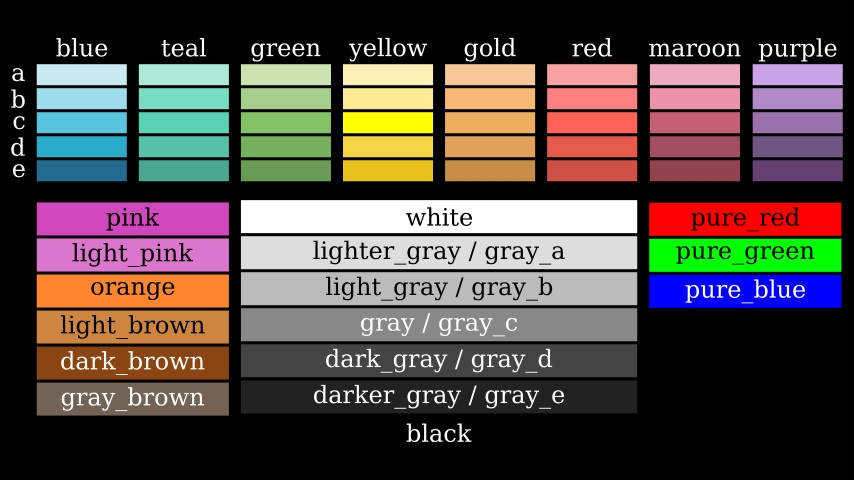
\includegraphics[width=0.8\textwidth]{part/图形化/manim/pic/基本图形/manim颜色.png}
    \caption{manim预置颜色}
    \label{fig:manim预置颜色}
\end{figure}


可以通过\codeinline{color}来设置图形的颜色。

\begin{lstlisting}[style=pythonstyle]
from manim import *

class ColorLineDemo(Scene):
    def construct(self):
        # 定义所有颜色系列及其不同深度
        color_groups = [
            [BLUE_E, BLUE_D, BLUE_C, BLUE_B, BLUE_A],        # blue 系列
            [TEAL_E, TEAL_D, TEAL_C, TEAL_B, TEAL_A],        # teal 系列
            [GREEN_E, GREEN_D, GREEN_C, GREEN_B, GREEN_A],   # green 系列
            [YELLOW_E, YELLOW_D, YELLOW_C, YELLOW_B, YELLOW_A], # yellow 系列
            [GOLD_E, GOLD_D, GOLD_C, GOLD_B, GOLD_A],        # gold 系列
            [RED_E, RED_D, RED_C, RED_B, RED_A],             # red 系列
            [MAROON_E, MAROON_D, MAROON_C, MAROON_B, MAROON_A], # maroon 系列
            [PURPLE_E, PURPLE_D, PURPLE_C, PURPLE_B, PURPLE_A], # purple 系列
            [PINK, LIGHT_PINK, ORANGE, LIGHT_BROWN, DARK_BROWN], # 单色系列
            [GRAY_BROWN, WHITE, LIGHTER_GRAY, LIGHT_GRAY, GRAY], # 灰色系列
            [DARK_GRAY, DARKER_GRAY, BLACK],                  # 深灰系列
            [PURE_RED, PURE_GREEN, PURE_BLUE]                # 纯色系列
        ]

        # 起始位置的 y 坐标
        y_start = 3
        # 每个颜色组的初始 x 坐标
        x_start = -6

        # 绘制每个颜色组及其深度
        for i, color_group in enumerate(color_groups):
            # 调整 x 坐标以便水平排列
            x_pos = x_start + (i * 1.6)
            for j, color in enumerate(color_group):
                # 创建每条线的y坐标偏移
                y_pos = y_start - (j * 0.6)
                line = Line(
                    [x_pos, y_pos, 0],
                    [x_pos + 1.2, y_pos, 0],
                    stroke_width=10,
                    color=color
                )
                # 动画显示线条
                self.play(Create(line), run_time=0.2)

        # 保持显示2秒
        self.wait(2)
\end{lstlisting}

\subsubsection{填充和透明度}
\label{subsubsec:Manim基本图形-填充和透明度}
可以通过\codeinline{fill\_color}和\codeinline{fill\_opacity}来设置图形的填充颜色和填充透明度。
\begin{lstlisting}[style=demostyle,numbers=none]
# 1.fill_color:
    类型: 字符串（颜色名称或十六进制颜色代码）
    描述: 指定图形的填充颜色。
    提示: 如果 fill_color 不是有效的颜色名称或十六进制颜色代码，则使用默认值 WHITE。

# 2.fill_opacity:
    类型: 浮点数或整数
    描述: 设置图形的填充透明度，取值范围为 0 到 1。
    默认值: 0
    提示: 如果 fill_opacity 小于 0 或大于 1，则使用默认值 0。
\end{lstlisting}

\begin{lstlisting}[style=pythonstyle]
# manim -pql 03Line_demo.py LineSample
from manim import *
class LineSample(Scene):
    def construct(self):
        self._lines()

    def _lines(self):
        # 1.创建简单的直线
        l1 = Line(
            [-1, 1, 0],
            [1, 1,0],
            fill_color=BLUE,
            fill_opacity=0.5,
            stroke_width=1,
        )
        self.play(Create(l1), run_time=0.5)

        l2 = Line(
            [-1, 0, 0],
            [1, 0, 0],
            fill_color=RED,
            fill_opacity=0.75,
            stroke_width=2,
        )
        self.play(Create(l2), run_time=0.5)

        c1 = Circle(
            radius=1,
            fill_color=BLUE,
            fill_opacity=0.5,
            stroke_width=1,
        )
        self.play(Create(c1), run_time=0.5)
\end{lstlisting}        


\section{坐标系}
\label{sec:Manim基本图形-坐标系}
没有引入坐标系之前，在绘制图形时，也有一个隐含的坐标系，它和屏幕的像素相关。

比如，我们之前示例中的各个图形，屏幕的中心就是坐标原点（$[0, 0]$）, 
横轴坐标的范围大概是 $[-3.5, 3.5]$，纵轴的坐标范围大概是 $[-4, 4]$，
这个范围与设置的视频分辨率有关，分辨率设置的越高的话，坐标范围越大。

\subsection{一维坐标系}
\label{subsec:Manim基本图形-一维坐标系}
数轴（\codeinline{NumberLine}）是最基本的一维坐标系，它的关键参数是
\begin{enumerate}[label=\arabic*)]
    \item \codeinline{x\_range}:设置数轴的范围和间隔
    \item \codeinline{length}:设置数轴的长度
\end{enumerate}
\begin{lstlisting}[style=pythonstyle]
# manim -pql 01NumberLineExample.py NumberLineExample
from manim import *

class NumberLineExample(Scene):
    def construct(self):
        # 第一条数轴：范围从 -10 到 10，步长为 2，长度为 10，包含数 字
        number_line_1 = NumberLine(
            x_range=[-10, 10, 2],  # 设置数轴范围为 -10 到 10，步长 为 2
            length=10,  # 设置数轴长度为 10
            include_numbers=True  # 在数轴上显示数字
        )
        number_line_1.to_edge(UP)  # 将第一条数轴移到屏幕上方

        # 第二条数轴：范围从 -3 到 3，步长为 0.5，长度为 12，包含数 字
        number_line_2 = NumberLine(
            x_range=[-3, 3, 0.5],  # 设置数轴范围为 -3 到 3，步长为 0.5
            length=12,  # 设置数轴长度为 12
            include_numbers=True  # 在数轴上显示数字
        )
        number_line_2.next_to(number_line_1, DOWN, buff=1)  # 将第二条数轴放在第一条数轴下方

        # 第三条数轴：范围从 -5 到 5，步长为 1，长度为 6，包含数字和箭头，旋转10度
        number_line_3 = NumberLine(
            x_range=[-5, 5 + 1, 1],  # 设置数轴范围为 -5 到 6，步长 为 1
            length=6,  # 设置数轴长度为 6
            include_numbers=True,  # 在数轴上显示数字
            include_tip=True,  # 在数轴的两端加上箭头
            rotation=10 * DEGREES  # 数轴旋转10度
        )
        number_line_3.next_to(number_line_2, DOWN, buff=1)  # 将第三条数轴放在第二条数轴下方

        # 动画显示三条数轴
        self.play(Create(number_line_1))
        self.play(Create(number_line_2))
        self.play(Create(number_line_3))

        # 保持场景显示2秒
        self.wait(2)

if __name__ == "__main__":
    from manim import config
    config.background_color = "#ffffff"  # 设置背景为白色
    scene = NumberLineExample()
    scene.render()
\end{lstlisting}           

\subsection{二维坐标系}
\label{subsec:Manim基本图形-二维坐标系}
\subsubsection{NumberPlane 实数平面}
\label{subsubsec:Manim基本图形-实数平面}
实数平面（\codeinline{NumberPlane}）是最基本的二绶坐标系，它的关键参数是
\begin{enumerate}[label=\arabic*)]
    \item \codeinline{x\_range}:设置\textcolor{YBXPurple}{X轴}横轴的范围和间隔
    \item \codeinline{y\_range}:设置\textcolor{YBXPurple}{Y轴}纵轴的范围和间隔
    \item \codeinline{x\_length}:设置\textcolor{YBXPurple}{X轴}横轴的长度
    \item \codeinline{y\_length}:设置\textcolor{YBXPurple}{Y轴}纵轴的长度
\end{enumerate}

\begin{lstlisting}[style=pythonstyle]
# manim -pql 01NumberPlaneExample.py NumberPlaneExample
from manim import *

class NumberPlaneExample(Scene):
    def construct(self):
        # 第一张网格：x 轴范围为 -4 到 11，y 轴范围为 -3 到 3，x 轴 长度为 3，y 轴长度为 2
        number_plane_1 = NumberPlane(
            x_range=(-4, 11, 1),  # 设置 x 轴范围为 -4 到 11，步长为 1
            y_range=(-3, 3, 1),   # 设置 y 轴范围为 -3 到 3，步长为 1
            x_length=3,  # 设置 x 轴的物理长度为 3
            y_length=2   # 设置 y 轴的物理长度为 2
        )
        number_plane_1.shift(LEFT * 2)  # 将第一张网格移到屏幕左侧

        # 第二张网格：x 轴范围为 -4 到 11，x 轴长度为 3，y 轴长度为 4（没有指定 y 轴范围）
        number_plane_2 = NumberPlane(
            x_range=(-4, 11, 1),  # 设置 x 轴范围为 -4 到 11，步长为 1
            x_length=3,  # 设置 x 轴的物理长度为 3
            y_length=4   # 设置 y 轴的物理长度为 4
        )
        number_plane_2.shift(RIGHT * 2)  # 将第二张网格移到屏幕右侧

        # 动画显示两张网格
        self.play(Create(number_plane_1))
        self.play(Create(number_plane_2))

        # 保持场景显示2秒
        self.wait(2)

if __name__ == "__main__":
    from manim import config
    config.background_color = "#ffffff"  # 设置背景为白色
    scene = NumberPlaneExample()
    scene.render()
\end{lstlisting}      

\subsubsection{ComplexPlane 复数平面}
\label{subsubsec:Manim基本图形-复数平面}

\begin{lstlisting}[style=pythonstyle]
# manim -pql 01ComplexPlaneExample.py ComplexPlaneExample
from manim import *

class ComplexPlaneExample(Scene):
    def construct(self):
        # 创建复平面，并添加坐标系
        plane = ComplexPlane().add_coordinates()

        # 创建第一个点，表示复数 2 + i，颜色为黄色
        d1 = Dot(plane.n2p(2 + 1j), color=YELLOW)  # 使用 n2p 将复数转换为平面上的点
        label1 = Tex("2+i").next_to(d1, UR, buff=0.1)  # 在点的右上 角添加标签 "2+i"

        # 创建第二个点，表示复数 -3 - 2i，颜色为黄色
        d2 = Dot(plane.n2p(-3 - 2j), color=YELLOW)  # 使用 n2p 将复 数转换为平面上的点
        label2 = Tex("-3-2i").next_to(d2, UR, buff=0.1)  # 在点的右 上角添加标签 "-3-2i"

        # 动画显示复平面、点和标签
        self.play(Create(plane))
        self.play(FadeIn(d1, label1))
        self.play(FadeIn(d2, label2))

        # 保持场景显示2秒
        self.wait(2)

if __name__ == "__main__":
    from manim import config
    config.background_color = "#fafafa"  # 设置浅色背景
    scene = ComplexPlaneExample()
    scene.render()
\end{lstlisting}        

\subsubsection{PolarPlane 极坐标平面}
\label{subsubsec:Manim基本图形-极坐标平面}
\codeinline{PolarPlane}是一个极坐标平面，它通过角度和与原点的距离来定位位置，经常被用于导航类的系统中， 与直角坐标相比，在这类系统中能极大的简化计算。 它的关键参数有：
\begin{enumerate}[label=\arabic*)]
    \item \codeinline{azimuth\_step}:分割的角度个数
    \item \codeinline{size}:极坐标在屏幕中显示的大小
    \item \codeinline{radius\_step}：极坐标半径的间隔
    \item \codeinline{radius\_max}：极坐标最大半径
\end{enumerate}


\begin{lstlisting}[style=pythonstyle]
# manim -pql 01PolarPlaneExample.py PolarPlaneExample
from manim import *

class PolarPlaneExample(Scene):
    def construct(self):
        # 创建极坐标平面
        plane = PolarPlane(
            azimuth_step=30,   # 设置方位角步长为 30 度
            size=6,            # 设置极坐标平面的大小为 6
            radius_step=1,      # 设置半径的步长为 1
            radius_max=3        # 设置最大半径为 3
        ).add_coordinates()     # 添加坐标轴的数字

        # 将极坐标平面居中放置
        plane.move_to(ORIGIN)

        # 动画显示极坐标平面
        self.play(Create(plane))

        # 保持场景显示2秒
        self.wait(2)

if __name__ == "__main__":
    from manim import config
    config.background_color = "#fafafa"  # 设置浅色背景
    scene = PolarPlaneExample()
    scene.render()
\end{lstlisting}      

\subsubsection{Axes 二维笛卡尔坐标轴}
\label{subsubsec:Manim基本图形-二维笛卡尔坐标轴}
二维的笛卡尔坐标系（\codeinline{Axes}）使用的比较多，它在平面坐标系之上，
又提供了更多的配置， 可以更加灵活的配置数轴，除了上面平面坐标系提到的那4个关键参数之外， 
还有2个配置坐标轴的参数也很重要：
\begin{enumerate}[label=\arabic*)]
    \item \codeinline{x\_axis\_config}:配置X轴如何显示的参数
    \item \codeinline{y\_axis\_config}:配置Y轴如何显示的参数
\end{enumerate}

\begin{lstlisting}[style=pythonstyle]
# manim -pql 01LogPlotExample.py LogPlotExample
from manim import *

class LogPlotExample(Scene):
    def construct(self):
        # 创建带有对数 y 轴的坐标系
        ax = Axes(
            x_range=[0, 10, 1],   # x 轴范围为 0 到 10，步长为 1
            y_range=[-2, 6, 1],   # y 轴范围为 -2 到 6，对数缩放
            x_length=6,           # x 轴长度为 6
            tips=False,           # 去掉轴的箭头
            axis_config={"include_numbers": True},  # 在轴上显示数字
            y_axis_config={"scaling": LogBase(custom_labels=True)},  # y 轴采用对数缩放
        )

        # 绘制 y = x^2 的函数曲线，注意 x_min 必须大于 0，因为 x=0  时，y 是负无穷
        graph = ax.plot(lambda x: x**2, x_range=[0.001, 10], use_smoothing=False)

        # 将坐标轴和函数曲线添加到场景中
        self.play(Create(ax), Create(graph))

        # 保持场景显示2秒
        self.wait(2)

if __name__ == "__main__":
    from manim import config
    config.background_color = "#ffffff"  # 设置浅色背景
    scene = LogPlotExample()
    scene.render()
\end{lstlisting}     



\subsection{三维坐标系}
\label{subsec:Manim基本图形-三维坐标系}
\subsubsection{ThreeDAxes 三维笛卡尔坐标系}
\label{subsubsec:Manim基本图形-三维笛卡尔坐标系}
三维的笛卡尔坐标系（\codeinline{ThreeDAxes}）与二维坐标系的参数类似，只是多了一个维度（Z轴）的配置， 其配置参数与X轴和Y轴类似。 
显示三维图形时，有2点需要额外注意，
\begin{enumerate}[label=\arabic*)]
    \item 场景要继承 \codeinline{ThreeDScene}
    \item 要调整下默认的相机位置，也就是视角的位置，默认视角是从Z轴顶部向下看的。
\end{enumerate}

\begin{lstlisting}[style=pythonstyle]
# manim -pql  01CoordinateSample.py  CoordinateSample
from manim import *

# 创建三维坐标轴并绘制一个蓝色圆形
class CoordinateSample(ThreeDScene):
    def construct(self):
        # 创建三维坐标轴，设置 y 轴的长度为 8
        axes = ThreeDAxes(y_length=8)

        # 创建一个蓝色的圆形，半径为 2
        circle = Circle(color=BLUE, radius=2)

        # 将坐标轴和圆形组合成一个 VGroup，以便同时显示
        vg = VGroup(axes, circle)

        # 默认的相机视角

        # 动画显示坐标轴和圆形
        self.play(Create(vg), run_time=2)

        # 暂停以查看最终场景
        self.wait()

# 运行场景
if __name__ == "__main__":
    from manim import config
    config.background_color = "#ffffff"  # 设置背景颜色为白色
    scene = CoordinateSample()
    scene.render()
\end{lstlisting}    

\begin{lstlisting}[style=pythonstyle]
# manim -pql  01CoordinateSample.py  CoordinateSample
from manim import *

# 创建三维坐标轴并绘制一个蓝色圆形
class CoordinateSample(ThreeDScene):
    def construct(self):
        # 创建三维坐标轴，设置 y 轴的长度为 8
        axes = ThreeDAxes(y_length=8)

        # 创建一个蓝色的圆形，半径为 2
        circle = Circle(color=BLUE, radius=2)

        # 将坐标轴和圆形组合成一个 VGroup，以便同时显示
        vg = VGroup(axes, circle)

        # 调整相机视角的代码 phi是与Z轴之间的角度，theta是围绕Z轴旋 转的角度
        self.set_camera_orientation(phi=75 * DEGREES, theta=30 * DEGREES)

        # 动画显示坐标轴和圆形
        self.play(Create(vg), run_time=2)

        # 暂停以查看最终场景
        self.wait()

# 运行场景
if __name__ == "__main__":
    from manim import config
    config.background_color = "#ffffff"  # 设置背景颜色为白色
    scene = CoordinateSample()
    scene.render()
\end{lstlisting}  


\begin{example}
    \exProblem
    实现全互联的神将网络
    \exSolution
    \begin{lstlisting}[style=pythonstyle]
    # manim -pql 02NeuralNetwoek_01.py
    from manim import *

    class NeuralNetwork(Scene):
        def construct(self):
            # 定义每一层的神经元数量
            #layer_sizes = [1, 8, 16, 8, 1]
            layer_sizes = [1, 8, 8, 1]
    
            # 定义每层神经元的位置
            layers = self.create_layers(layer_sizes)
    
            # 连接所有层的节点
            self.connect_layers(layers)
    
            # 保持显示
            self.wait(2)
    
        def create_layers(self, layer_sizes):
            """
            创建每一层的神经元，并返回各层的节点集合
            """
            layers = []
            x_position = -5  # 起始x坐标
            for layer_size in layer_sizes:
                layer = self.create_layer(layer_size, x_position)
                layers.append(layer)
                x_position += 2  # 各层间隔
    
            return layers
    
        def create_layer(self, layer_size, x_position):
            """
            创建单层神经元，并返回该层的节点集合
            """
            layer = VGroup()  # 创建一个组来包含这一层的所有节点
            y_start = -(layer_size - 1) / 2  # 起始y坐标
            for i in range(layer_size):
                neuron = Circle(radius=0.2, color=WHITE)  # 创建一个神经元（圆形）
                neuron.move_to([x_position, y_start + i, 0])  # 移动到指定位置
                layer.add(neuron)
                self.play(Create(neuron), run_time=0.1)  # 动画显示神经 元
    
            return layer
    
        def connect_layers(self, layers):
            """
            连接相邻层之间的所有神经元
            """
            for i in range(len(layers) - 1):
                layer1 = layers[i]
                layer2 = layers[i + 1]
                for neuron1 in layer1:
                    for neuron2 in layer2:
                        connection = Line(neuron1.get_center(), neuron2.get_center(), stroke_width=1, color=WHITE)
                        self.play(Create(connection), run_time=0.05)  # 动画显示连接线
    \end{lstlisting}
\end{example}



\chapter{Manim文字和公式}
\label{cha:manim_text_formula}
\section{Text文字}
\label{sec:manim_text_formula_text}
Text系列常用的对象主要有三种：
\begin{enumerate}[label=\arabic*)]
    \item Text：一般用于单行的文本
    \item Paragraph：一般用于多行的文本
    \item MarkupText：一般用于富文本显示
\end{enumerate}

\subsection{一般文本}
\label{subsec:manim_text_formula_text_general}
\begin{lstlisting}[style=pythonstyle]
# manim -pql 01TextSample.py TextSample
from  manim import *

class TextSample(Scene):
    def construct(self):
        text1 = Text("Hello, World!")
        self.play(Write(text1))
        text2 = Text("Hello, World!", font="Arial")
        self.play(ReplacementTransform(text1, text2))
        self.play(FadeOut(text2))

        # 创建不同语言的文本
        english_text = Text("hello world")  # 英文
        chinese_text = Text("你好，世界")    # 中文
        japanese_text = Text("こんにちは世界") # 日文
        russian_text = Text("Привет, мир")   # 俄文
        arabic_text = Text("مرحبا بالعالم", font="sans-serif") # 阿拉伯文
        # 对文本进行位置调整，使其按顺序排列
        english_text.to_edge(UP * 2)
        chinese_text.next_to(english_text, DOWN, buff=0.5)
        japanese_text.next_to(chinese_text, DOWN, buff=0.5)
        russian_text.next_to(japanese_text, DOWN, buff=0.5)
        arabic_text.next_to(russian_text, DOWN, buff=0.5)
        # 将所有文本依次显示到场景中
        self.play(Write(english_text))
        self.play(Write(chinese_text))
        self.play(Write(japanese_text))
        self.play(Write(russian_text))
        self.play(Write(arabic_text))

        self.wait(2)
\end{lstlisting}      

\subsection{多行文本}
\label{subsec:manim_text_formula_text_paragraph}
\begin{lstlisting}[style=pythonstyle]
# manim -pql 01ParagraphSample.py ParagraphSample
from manim import *

class ParagraphSample(Scene):
    def construct(self):
        # 创建包含古诗的 Paragraph 对象
        paragraph = Paragraph(
            "   春晓\n",         # 标题
            "春眠不觉晓",         # 第一行
            "处处闻啼鸟",         # 第二行
            "夜来风雨声",         # 第三行
            "花落知多少",         # 第四行
            alignment="center"   # 文本居中对齐
        )

        # 设置诗的标题样式
        title = paragraph[0]  # 提取标题部分
        title.set_color(YELLOW)  # 设置标题颜色

        # 动画显示古诗
        self.play(Write(paragraph, run_time=3))
        
        # 保持场景显示2秒
        self.wait(2)
\end{lstlisting}        

\subsection{富文本}
\label{subsec:manim_text_formula_text_markup}
使用 \codeinline{MarkupText} 类来创建带有 HTML 样式的文本。
\begin{enumerate}[label=\arabic*)]
    \item \codeinline{<b>...</b>}：加粗
    \item \codeinline{<i>...</i>}：斜体
    \item \codeinline{<u>...</u>}：下划线
    \item \codeinline{<s>...</s>}：中划线
    \item \codeinline{<span underline="double">...</span>}：双下划线
    \item \codeinline{<span underline="error">...</span>}：错误标记（通常是红色波浪线）
    \item \codeinline{<sub>...</sub>}：下标
    \item \codeinline{<sup>...</sup>}：上标
\end{enumerate}

设置位置
\begin{enumerate}[label=\arabic*)]
    \item \codeinline{to\_edge()}：设置文本的位置
    \item \codeinline{next\_to()}：设置文本相对于另一个对象的位置
    \item \codeinline{shift()}：设置文本的位置偏移
    \item \codeinline{move\_to()}：设置文本的位置
    \item \codeinline{scale()}：设置文本的缩放比例
\end{enumerate}

\begin{lstlisting}[style=pythonstyle]
# manim -pql 01MarkupTextDemo.py MarkupTextDemo

from manim import *

class MarkupTextDemo(Scene):
    def construct(self):
        # 创建不同样式的文本对象
        bold_italic_text = MarkupText("<b>bold</b> <i>斜体文字</i>")
        underline_strike_text = MarkupText("<u>下划线</u> <s>中划线</s>")
        double_underline_error = MarkupText(
            '<span underline="double">双下划线</span> <span underline="error">错误标记</span>'
        )
        subscript_superscript = MarkupText("下标和上标：H<sub>2</sub>O H<sub>3</sub>O<sup>+</sup>")

        # 设置每个文本的位置
        bold_italic_text.to_edge(UP * 2)
        underline_strike_text.next_to(bold_italic_text, DOWN, buff=0.5)
        double_underline_error.next_to(underline_strike_text, DOWN, buff=0.5)
        subscript_superscript.next_to(double_underline_error, DOWN, buff=0.5)

        # 动画显示文本
        self.play(Write(bold_italic_text))
        self.play(Write(underline_strike_text))
        self.play(Write(double_underline_error))
        self.play(Write(subscript_superscript))

        # 保持显示2秒
        self.wait(2)
\end{lstlisting}        


\section{Tex公式}
\label{sec:manim_text_formula_formula}
Tex系列的对象主要是用来显示数学公式，
基于Tex之上，manim还封装了列表和标题两种常用的对象。

不过，Tex默认\textcolor{red}{\textbf{只}}支持显示英文，所以多用于显示公式，
显示文本还是 \codeinline{Text} 系列的对象比较常用。

\subsection{公式}
\label{subsec:manim_text_formula_formula_formula}
\codeinline{Tex} 可以显示任何 Latex格式的数学公式：

\begin{lstlisting}[style=pythonstyle]
# manim -pql 01MathEquations.py MathEquations    
from manim import *

class MathEquations(Scene):
    def construct(self):
        # 创建不同的数学公式
        pythagorean = Tex(r"$a^2 + b^2 = c^2$")
        einstein = Tex(r"$E = mc^2$")
        euler = Tex(r"$e^{i\pi} + 1 = 0$")

        # 设置每个公式的位置
        pythagorean.to_edge(UP * 2)
        einstein.next_to(pythagorean, DOWN, buff=0.5)
        euler.next_to(einstein, DOWN, buff=0.5)

        # 动画显示公式
        self.play(Write(pythagorean))
        self.play(Write(einstein))
        self.play(Write(euler))

        # 保持显示2秒
        self.wait(2)
\end{lstlisting}

\subsection{列表}
\label{subsec:manim_text_formula_formula_list}
\codeinline{BulletedList}会将传入的多个字符串以列表的方式排列起来

\begin{lstlisting}[style=pythonstyle]
# manim -pql 01MathListDemo.py MathListDemo   
from manim import *

class MathListDemo(Scene):
    def construct(self):
        # 创建包含数学公式的项目符号列表
        bulleted_list = BulletedList(
            r"$a^2 + b^2 = c^2$",   # 毕达哥拉斯定理
            r"$E = mc^2$",          # 爱因斯坦质能方程
            r"$e^{i\pi} + 1 = 0$"   # 欧拉公式
        )

        # 将列表居中显示
        bulleted_list.scale(1.5)  # 调整文本大小以便更好展示

        # 动画展示项目符号列表
        self.play(Write(bulleted_list))

        # 保持显示2秒
        self.wait(2)
\end{lstlisting}

\subsection{标题}
\label{subsec:manim_text_formula_formula_title}
\codeinline{Title} 会将传入的字符串以标题的方式展示出来。

\begin{lstlisting}[style=pythonstyle]
# manim -pql 01TitleDemo.py TitleDemo   
from manim import *
import manim

class TitleDemo(Scene):
    def construct(self):
        # 获取当前 Manim 版本号
        version_text = f"Manim version {manim.__version__}"

        # 创建标题对象
        title = Title(version_text)

        # 动画显示标题
        self.play(Write(title))

        # 保持显示2秒
        self.wait(2)
\end{lstlisting} 

\codeinline{Title} 类基于 LaTeX 渲染器，而在渲染中文时，
LaTeX 的默认设置可能无法正确处理中文字符，因此会导致 LaTeX 编译错误。
为了解决这个问题，我们可以使用 Title 类中的 Tex 模式来处理非中文字符，
而对于中文文本则使用 \codeinline{Text} 类。

\begin{lstlisting}[style=pythonstyle]
from manim import *

class FEMHistory(Scene):
    def construct(self):
        #1. 定义有限元方法的历史事件
        history = [
            "1943年: 结构工程师柯朗提出有限元方法的早期概念。",
            "1956年: Turner等人正式提出有限元方法，用于解决结构分析 问题。",
            "1960年代: 有限元方法被广泛应用于结构力学、热传导和流体 力学领域。",
            "1970年代: 有限元方法理论化，逐渐推广到非线性问题和复杂 几何形状。",
            "1980年代: 高性能计算的发展推动了大型有限元模型的应用。",
            "1990年代: 有限元方法成为工程、航空航天、汽车等行业的标 准工具。",
            "2000年后: 有限元方法与其他数值方法结合，如多尺度模拟和 优化。"
        ]

        # 2.创建标题
        # 1) 使用Title显示英文标题
        #title = Title("FEM History").scale(1.2)  # 使用Title只能显 示英文
        # 2) 使用Text显示中文标题
        # (1)创建标题
        title = Text("有限元方法的发展历史", font="SimSun").scale(1.2)  # SimSun 字体支持中文
        # (2)获取标题的宽度并创建下划线
        underline = Line(
            start=[-title.width / 2, -0.1, 0],  # 根据标题宽度设置下划线的起始点
            end=[title.width / 2, -0.1, 0],    # 下划线的终止点
            stroke_width=2,                    # 下划线的宽度
            color=WHITE                        # 下划线颜色为白色
        )
        # (3)将标题与下划线组合成一个VGroup，便于统一操作
        title_group = VGroup(title, underline).arrange(DOWN, buff=0.2)

        # 3.播放动画
        # self.play(FadeIn(title))      # 显示Title
        self.play(FadeIn(title_group))  # 显示Text标题
        self.wait(1)
        #self.play(title.animate.to_edge(UP))
        self.play(title_group.animate.to_edge(UP))

        # 4.动画显示每个历史事件
        for event in history:
            event_text = Text(event, font="SimSun", font_size=24)
            self.play(FadeIn(event_text))
            self.wait(2)
            self.play(FadeOut(event_text))

        # 5.结束语
        thank_you = Text("感谢观看！", font="SimSun").scale(1.2)
        self.play(FadeIn(thank_you))
        self.wait(2)

if __name__ == "__main__":
    from manim import *
    scene = FEMHistory()
    scene.render()
\end{lstlisting}  

\section{文本样式}
\label{sec:manim_text_formula_style}
Manim 支持自定义文本样式，允许用户修改字体、大小、颜色等属性。

\begin{table}[htpb]
\begin{tabular}{c|c}
属性              & 备注                                \\ \hline
font\_size        & 字体大小，默认为48                   \\
font              & 字体名称，例如 "Arial" 或 "SimSun"    \\
color             & 文本颜色，默认为白色                 \\
gradient          & 渐变颜色，可以指定多个颜色            \\
slant             & 倾斜角度，选项有 ITALIC（斜体）         \\
weight            & 字重，选项有 BOLD（粗体）             \\
t2c               & 给定文字的特定部分自定义颜色         \\
line\_spacing     & 文本行间距                          \\
alignment         & 文本对齐方式，选项有 "center", "left" 等 \\
\end{tabular}
\caption{manim中的文字样式}
\label{tab:manim中的文字样式}
\end{table}

\subsection{颜色相关}
\label{subsec:manim_text_formula_style_color}
\subsubsection{color 单色}
\label{subsubsec:manim_text_formula_style_color_single}

\begin{lstlisting}[style=pythonstyle]
# manim -pql 02TextAndMathDemo.py TextAndMathDemo
from manim import *

class TextAndMathDemo(Scene):
    def construct(self):
        # 创建各种文本和数学公式对象，并为它们指定不同的颜色
        text_english = Text("hello world", color=RED)
        text_chinese = Text("你好，世界", color=YELLOW)
        text_japanese = Text("こんにちは世界", color=GREEN)

        tex_pythagoras = Tex(r"$a^2 + b^2 = c^2$", color=RED)
        tex_einstein = Tex(r"$E = mc^2$", color=YELLOW)
        tex_euler = Tex(r"$e^{i\pi} + 1 = 0$", color=GREEN)

        # 设置每个文本和公式的位置
        text_english.to_edge(UP)
        text_chinese.next_to(text_english, DOWN)
        text_japanese.next_to(text_chinese, DOWN)

        tex_pythagoras.next_to(text_japanese, DOWN, buff=1)
        tex_einstein.next_to(tex_pythagoras, DOWN)
        tex_euler.next_to(tex_einstein, DOWN)

        # 依次显示文本和公式
        self.play(Write(text_english))
        self.play(Write(text_chinese))
        self.play(Write(text_japanese))

        self.play(Write(tex_pythagoras))
        self.play(Write(tex_einstein))
        self.play(Write(tex_euler))

        # 保持场景显示一段时间
        self.wait(2)

if __name__ == "__main__":
    from manim import config
    config.background_color = "#fafafa"  # 可选：设置背景颜色
    scene = TextAndMathDemo()
    scene.render()
\end{lstlisting}

\subsubsection{gradient 渐变色}
\label{subsubsec:manim_text_formula_style_color_gradient}
\codeinline{set\_color\_by\_gradient} 方法可以为文本和公式设置渐变颜色。

\begin{lstlisting}[style=pythonstyle]
from manim import *

class GradientTextAndMath(Scene):
    def construct(self):
        # 创建英文文本并设置渐变颜色
        text_english = Text("hello world").set_color_by_gradient(RED, GREEN)
        # 创建中文文本并设置渐变颜色
        text_chinese = Text("你好，世界").set_color_by_gradient(YELLOW, BLUE)
        # 创建日文文本并设置渐变颜色
        text_japanese = Text("こんにちは世界").set_color_by_gradient(BLUE, RED)

        # 创建数学公式并设置渐变颜色
        tex_pythagoras = Tex(r"$a^2 + b^2 = c^2$").set_color_by_gradient(RED, GREEN)
        tex_einstein = Tex(r"$E = mc^2$").set_color_by_gradient(YELLOW, BLUE)
        tex_euler = Tex(r"$e^{i\pi} + 1 = 0$").set_color_by_gradient(BLUE, RED)

        # 设置每个文本和公式的位置
        text_english.to_edge(UP)  # 将英文文本移至屏幕上方
        text_chinese.next_to(text_english, DOWN, buff=0.5)  # 中文文本在英文下方
        text_japanese.next_to(text_chinese, DOWN, buff=0.5)  # 日文 文本在中文下方

        tex_pythagoras.next_to(text_japanese, DOWN, buff=1)  # 数学 公式在文本下方
        tex_einstein.next_to(tex_pythagoras, DOWN, buff=0.5)  # 公式E=mc^2在其下方
        tex_euler.next_to(tex_einstein, DOWN, buff=0.5)  # 欧拉公式 在最下方

        # 使用动画依次显示文本和公式
        self.play(Write(text_english))
        self.play(Write(text_chinese))
        self.play(Write(text_japanese))

        self.play(Write(tex_pythagoras))
        self.play(Write(tex_einstein))
        self.play(Write(tex_euler))

        # 保持场景显示2秒
        self.wait(2)

if __name__ == "__main__":
    from manim import config
    config.background_color = "#fafafa"  # 设置浅色背景
    scene = GradientTextAndMath()
    scene.render()
\end{lstlisting}

\subsubsection{按字符设置颜色}
\label{subsubsec:manim_text_formula_style_color_char}

\begin{enumerate}[label=\arabic*)]
    \item 文本的颜色设置：\codeinline{t2c}：给定文字的特定部分自定义颜色

    \begin{lstlisting}[style=pythonstyle]
    # manim -pql 02TextWithColor.py
    from manim import *

    class TextAndMathWithColors(Scene):
        def construct(self):
            # 文本的颜色设置
            text = Text("JLU.com", t2c={"JL": BLUE, "U": RED, "com": GREEN})
            text.to_edge(UP)  # 将文本移到屏幕的上边缘
    
            text2 = Text("我爱计算机", t2c={"我": BLUE, "爱": RED, "计算机": GREEN})
    
    
            # 动画显示文本和公式
            self.play(Write(text))
            self.wait(1)
            self.play(ReplacementTransform(text, text2))
    
            # 保持场景显示2秒
            self.wait(2)
    
    if __name__ == "__main__":
        from manim import config
        config.background_color = "#ffffff"  # 设置白色背景
        scene = TextAndMathWithColors()
        scene.render()
    \end{lstlisting}

    \item LaTeX 数学公式的颜色设置 
    \begin{lstlisting}[style=pythonstyle]
    # manim -pql 02TextWithColor.py
    from manim import *

    class TextAndMathWithColors(Scene):
        def construct(self):
            # LaTeX 数学公式的颜色设置
            tex = Tex(r"$a^2$", " + ", r"$b^2$", " = ", r"$c^2$")
            # 分别为公式中的不同部分设置颜色
            tex.set_color_by_tex("a^2", RED)
            tex.set_color_by_tex("b^2", YELLOW)
            tex.set_color_by_tex("c^2", GREEN)
    
            # 动画显示文本和公式
            self.play(Write(tex))
    
            # 保持场景显示2秒
            self.wait(2)
    
    if __name__ == "__main__":
        from manim import config
        config.background_color = "#ffffff"  # 设置白色背景
        scene = TextAndMathWithColors()
        scene.render()
    \end{lstlisting}
\end{enumerate}


\subsection{字体相关}
\label{subsec:manim_text_formula_style_font}
\subsubsection{font 字体}
\label{subsubsec:manim_text_formula_style_font_font}
manim通过 \codeinline{font} 属性设置字体。

\begin{lstlisting}[style=pythonstyle]
# manim -pql 01CustomFontText.py CustomFontText    
from manim import *

class CustomFontText(Scene):
    def construct(self):
        # 英文文本，使用 Consolas 字体
        text_english = Text("I love", font="Consolas")
        text_english.to_edge(UP)  # 将文本移到屏幕的上方

        # 中文文本，使用华文行楷字体
        text_chinese_xingkai = Text("数学", font="STXingkai")  # 华 文行楷字体
        text_chinese_xingkai.next_to(text_english, DOWN, buff=0.5)  # 将中文放在英文下方

        # 中文文本，使用华文彩云字体
        text_chinese_caiyun = Text("计算机", font="STCaiyun")  # 华 文彩云字体
        text_chinese_caiyun.next_to(text_chinese_xingkai, DOWN, buff=0.5)  # 将“之旅”放在“数学”下方

        # 动画依次显示文本
        self.play(Write(text_english))
        self.play(Write(text_chinese_xingkai))
        self.play(Write(text_chinese_caiyun))

        # 保持场景显示2秒
        self.wait(2)

if __name__ == "__main__":
    from manim import config
    config.background_color = "#fafafa"  # 设置浅色背景
    scene = CustomFontText()
    scene.render()
\end{lstlisting}    

引用本地字体文件

\subsubsection{font\_size 字体大小}
\label{subsubsec:manim_text_formula_style_font_fontsize}
\begin{lstlisting}[style=pythonstyle]
# manim -pql  01TextWithDifferentSize.py TextWithDifferentSizes
from manim import *

class TextWithDifferentSizes(Scene):
    def construct(self):
        # 创建不同大小的文本
        text_1 = Text("I", font_size=20)         # 字体大小为20
        text_2 = Text("love", font_size=30)      # 字体大小为30
        text_3 = Text("数学", font_size=40)       # 字体大小为40，中文字符
        text_4 = Text("&", font_size=50)         # 字体大小为50
        text_5 = Text("计算机", font_size=60)     # 字体大小为60，中文字符

        # 调整文本位置，使它们按顺序显示在同一行上
        text_1.to_edge(LEFT)  # 将"I"移到屏幕左边缘
        text_2.next_to(text_1, RIGHT, buff=0.5)  # "love" 放在 "I"  的右边，间隔0.5
        text_3.next_to(text_2, RIGHT, buff=0.5)  # "数学" 放在 "love" 的右边，间隔0.5
        text_4.next_to(text_3, RIGHT, buff=0.5)  # "&" 放在 "数学"  的右边，间隔0.5
        text_5.next_to(text_4, RIGHT, buff=0.5)  # "计算机" 放在 "&" 的右边，间隔0.5

        # 依次显示每个文本
        self.play(Write(text_1))
        self.play(Write(text_2))
        self.play(Write(text_3))
        self.play(Write(text_4))
        self.play(Write(text_5))

        # 保持场景显示2秒
        self.wait(2)

if __name__ == "__main__":
    from manim import config
    config.background_color = "#fafafa"  # 设置浅色背景
    scene = TextWithDifferentSizes()
    scene.render()
\end{lstlisting}    

\subsubsection{weight 字重}
\label{subsubsec:manim_text_formula_style_font_weight}
\begin{lstlisting}[style=pythonstyle]
# manim -pql 01TextWithDifferentWeights.py TextWithDifferentWeights
from manim import *

class TextWithDifferentWeights(Scene):
    def construct(self):
        # 正常字体权重的英文文本
        text_normal = Text("NORMAL font weight")  # 正常字体
        text_normal.to_edge(UP)  # 将文本移到屏幕的上方

        # 加粗字体权重的英文文本
        text_bold_english = Text("BOLD font weight", weight=BOLD)  # 加粗字体
        text_bold_english.next_to(text_normal, DOWN, buff=0.5)  # 在正常字体下方显示

        # 正常字体权重的中文文本，使用宋体
        text_normal_chinese = Text("正常字重", font="SimSun")  # 正 常宋体
        text_normal_chinese.next_to(text_bold_english, DOWN, buff=0.5)  # 在英文加粗字体下方显示

        # 加粗字体权重的中文文本
        text_bold_chinese = Text("加粗字体", font="SimSun", weight=BOLD)  # 加粗宋体
        text_bold_chinese.next_to(text_normal_chinese, DOWN, buff=0.5)  # 在正常中文字体下方显示

        # 依次显示每个文本
        self.play(Write(text_normal))
        self.play(Write(text_bold_english))
        self.play(Write(text_normal_chinese))
        self.play(Write(text_bold_chinese))

        # 保持场景显示2秒
        self.wait(2)

if __name__ == "__main__":
    from manim import config
    config.background_color = "#fafafa"  # 设置浅色背景
    scene = TextWithDifferentWeights()
    scene.render()
\end{lstlisting}       

\subsubsection{slant 倾斜}
\label{subsubsec:manim_text_formula_style_font_slant}

\begin{lstlisting}[style=pythonstyle]
#  manim -pql 01TextWithItalicAndNormal.py TextWithItalicAndNormal       
from manim import *

class TextWithItalicAndNormal(Scene):
    def construct(self):
        # 正常字体权重的英文文本
        text_normal = Text("NORMAL font weight")  # 正常字体
        text_normal.to_edge(UP)  # 将文本移到屏幕的上方

        # 斜体字体权重的英文文本
        text_italic_english = Text("ITALIC font", slant=ITALIC)  #  斜体字体
        text_italic_english.next_to(text_normal, DOWN, buff=0.5)  # 在正常字体下方显示

        text_bold_itatic = Text("BOLD ITALIC", slant=ITALIC, weight=BOLD)  # 粗斜体字体
        text_bold_itatic.next_to(text_italic_english, DOWN, buff=0.5)

        # 正常字体权重的中文文本，使用宋体
        text_normal_chinese = Text("正常字重", font="SimSun")  # 正 常宋体
        text_normal_chinese.next_to(text_bold_itatic, DOWN, buff=0.5)

        # 斜体字体权重的中文文本
        text_italic_chinese = Text("斜体", font="SimSun", slant=ITALIC)  # 斜体宋体
        text_italic_chinese.next_to(text_normal_chinese, DOWN, buff=0.5)  # 在正常中文字体下方显示

        # 斜体加粗字体权重的中文文本
        text_bold_italic_chinese = Text("粗斜体", font="SimSun", slant=ITALIC, weight=BOLD)
        text_bold_italic_chinese.next_to(text_italic_chinese, DOWN, buff=0.5)

        # 依次显示每个文本
        self.play(Write(text_normal))
        self.play(Write(text_italic_english))
        self.play(Write(text_bold_itatic))
        self.play(Write(text_normal_chinese))
        self.play(Write(text_italic_chinese))
        self.play(Write(text_bold_italic_chinese))


        # 保持场景显示2秒
        self.wait(2)

if __name__ == "__main__":
    from manim import config
    config.background_color = "#fafafa"  # 设置浅色背景
    scene = TextWithItalicAndNormal()
    scene.render()
\end{lstlisting}       



\subsubsection{按字符设置}
\label{subsubsec:manim_text_formula_style_font_char}
\begin{enumerate}[label=\arabic*)]
    \item \codeinline{t2f}：按字符设置字体
    \item \codeinline{t2s}：按字符设置斜体
    \item \codeinline{t2w}：按字符设置粗体
\end{enumerate}

\begin{lstlisting}[style=pythonstyle]
# manim -pql 01TextWithStyles.py TextWithStyles
from manim import *

class TextWithStyles(Scene):
    def construct(self):
        # 创建带有不同样式的文本
        text = Text(
            "I love 数学计算机",  # 目标文本
            t2f={"数学": "STXingkai", "之旅": "SimSun"},  # 为"数学"部分使用STXingkai字体，为"之旅"使用SimSun字体
            t2s={"I": ITALIC},  # 将"ma"部分设置为斜体
            t2w={"love": BOLD},   # 将"nim"部分设置为加粗
        )

        # 将文本放置在屏幕中央
        text.move_to(ORIGIN)

        # 动画显示文本
        self.play(Write(text))

        # 保持场景显示2秒
        self.wait(2)

if __name__ == "__main__":
    from manim import config
    config.background_color = "#fafafa"  # 设置浅色背景
    scene = TextWithStyles()
    scene.render()
\end{lstlisting}  



\chapter{manim动画效果}
\label{cha:manim_animation}

\section{创建}
\label{sec:manim_animation_create}
展示某个元素或者文字时，一下子就全显示出来会显得比较突兀，通过创建效果的动画，让各个元素的出现更加的自然。 常用的创建效果动画主要有：
\begin{enumerate}[label=\arabic*)]
    \item \codeinline{Create()}：创建效果，元素从无到有。
    \item \codeinline{Write()}：书写效果，元素逐渐显示。
    \item \codeinline{FadeIn()}：淡入效果，元素从透明到不透明。
\end{enumerate}

\subsection{Create 创建图形}
\label{subsubsec:manim_animation_create_create}
\codeinline{Create()} 用于创建图形，绘制时图形逐步显示出来。例如，创建一个圆形：
\begin{lstlisting}[style=pythonstyle]
# manim -pql 01CreateCircle.py
from manim import *

class CreateCircle(Scene):
    def construct(self):
        circle = Circle()
        self.play(Create(circle))
\end{lstlisting}

\begin{lstlisting}[style=pythonstyle]
# manim -pql 01CreateSquare.py CreateSquare
from manim import *
class CreateSquare(Scene):
    def construct(self):
        s = Square(side_length=2, color=BLUE)
        self.play(Create(s))
\end{lstlisting}

\subsection{Write 书写效果}
\label{subsubsec:manim_animation_create_write}
\begin{lstlisting}[style=pythonstyle]
# manim -pql 02WriteText.py WriteText
from manim import *

class WriteText(Scene):
    def construct(self):
        text = Text(
            "Welcome to Manim",
            t2c={"Welcome": BLUE, "Manim": RED},
            t2f={"Manim": "STCaiyun"},
        )
        self.play(Write(text))
\end{lstlisting}    

\subsection{FadeIn 淡入效果}
\label{subsubsec:manim_animation_create_fadein}
\begin{lstlisting}[style=pythonstyle]
# manim -pql 01FadeInExample.py FadeInExample
from manim import *

# 使用不同的类名以避免与 Manim 内置类的冲突
class FadeInExample(Scene):
    def construct(self):
        # 创建文本对象
        text = Text("Welcome to Manim")

        # 渐入显示文本
        self.play(FadeIn(text))
        self.wait(2)

        # 渐出文本
        self.play(FadeOut(text))

        # 创建一个蓝色的正方形
        square = Square(side_length=2, color=BLUE, fill_opacity=0.6)

        # 渐入显示正方形
        self.play(FadeIn(square))
        self.wait(2)
\end{lstlisting}

\subsection{add 添加元素}
\label{subsubsec:manim_animation_create_add}
\codeinline{add()} 方法用于添加元素，可以一次添加多个元素。没有动画效果，元素会立即显示出来。

例如，添加一个圆形和一个正方形：
\begin{lstlisting}[style=pythonstyle]
# manim -pql 01AddExample.py AddExample
from manim import *

class AddExample(Scene):
    def construct(self):
        # 创建两个对象
        circle = Circle(color=BLUE)
        square = Square(side_length=2, color=RED)

        # 添加对象
        self.add(circle, square)
\end{lstlisting}

\section{销毁}
\label{sec:manim_animation_destroy}
销毁的效果一般用在移除图形和文字的场合。

\subsection{Uncreate 擦除图形}
\label{subsubsec:manim_animation_destroy_uncreate}
\begin{lstlisting}[style=pythonstyle]
# manim -pql 02UncreateSquare.py UncreateSquare
from manim import *

class UncreateSquare(Scene):
    def construct(self):
        square = Square(side_length=2, color=BLUE)
        self.add(square)
        self.wait(0.5)
        self.play(Uncreate(square))
\end{lstlisting}

\subsection{Unwrite 擦除文字}
\label{subsubsec:manim_animation_destroy_unwrite}
\begin{lstlisting}[style=pythonstyle]
# manim -pql 02UnwriteText.py UnwriteText
from manim import *

class UnwriteText(Scene):
    def construct(self):
        text = Text(
            "Welcome to Manim",
            t2c={"Welcome": BLUE, "Manim": RED},
            t2f={"Manim": "STCaiyun"},
        )
        self.add(text)
        self.wait(0.5)
        self.play(Unwrite(text))
\end{lstlisting}

\subsection{FadeOut 淡出效果}
\label{subsubsec:manim_animation_destroy_fadeout}
\begin{lstlisting}[style=pythonstyle]
# manim -pql 02FadeOutExample.py FadeOutExample
from manim import *

class FadeOutExample(Scene):
    def construct(self):
        # 创建两个对象
        circle = Circle(color=BLUE)
        square = Square(side_length=2, color=RED)

        # 渐出对象
        self.play(FadeOut(circle))
        self.wait(0.5)
        self.play(FadeOut(square))
\end{lstlisting}

\section{移动}
\label{sec:manim_animation_move}
\subsection{shift 移动指定距离}
\label{subsubsec:manim_animation_move_shift}
\begin{lstlisting}[style=pythonstyle]
# manim -pql 03ShiftExample.py ShiftExample
from manim import *
class ShiftExample(Scene):
    def construct(self):
        # 创建两个对象
        circle = Circle(color=RED)
        square = Square(side_length=1, color=BLUE, fill_opacity=0.6)

        # 移动指定距离
        self.play(circle.animate.shift(UP))     # 上移1个单位
        self.play(circle.animate.shift(RIGHT))  # 右移1个单位
        self.play(circle.animate.shift(DOWN*3)) # 下移3个单位
        self.play(circle.animate.shift(LEFT*2)) # 左移2个单位
        self.wait(0.5)
\end{lstlisting}


\subsection{move\_to 移动到指定位置}
\label{subsubsec:manim_animation_move_moveto}
\begin{lstlisting}[style=pythonstyle]
# manim -pql 03MoveToExample.py MoveToExample
from manim import *

class MoveToExample(Scene):
    def construct(self):
        # 创建两个对象
        circle = Circle(color=BLUE)
        square = Square(side_length=2, color=RED)

        # 移动到指定位置
        self.play(circle.animate.move_to(LEFT))
        self.wait(0.5)
        self.play(circle.animate.move_to(UP))
        self.wait(0.5)
        self.play(circle.animate.move_to(RIGHT))
        self.wait(0.5)
        self.play(circle.animate.move_to(DOWN))
        self.wait(0.5)
        self.play(circle.animate.move_to(ORIGIN))
        self.wait(0.5)
        self.play(square.animate.move_to(RIGHT))
        self.wait(0.5)
        self.play(square.animate.move_to(ORIGIN))
        self.wait(0.5)
        self.play(square.animate.move_to(ORIGIN+UP))
        self.wait(0.5)

\end{lstlisting}

\subsection{MoveAlongPath 沿路径移动}
\label{subsubsec:manim_animation_move_movealongpath}
常用的动画一般都是直线运动或者圆弧运动，而 \codeinline{MoveAlongPath} 可以让元素沿着任意的函数轨迹来运动。

\begin{lstlisting}[style=pythonstyle]
# manim -pql 01CosineGraph.py CosineGraph
from manim import *
import numpy as np

class CosineGraph(Scene):
    def construct(self):
        # 创建一个复杂的余弦函数图像
        cos_func = FunctionGraph(
            lambda t: np.cos(t) + 0.5 * np.cos(7 * t) + (1 / 7) * np.cos(14 * t),
            color=RED,  # 设定图像的颜色为红色
            x_range=[-PI, PI],  # 设定x轴的范围
        )
        
        # 将函数图像添加到场景中
        self.add(cos_func)
        
        # 创建一个点并放置在曲线的起点位置
        d1 = Dot(cos_func.get_start(), color=BLUE)
        
        # 将点添加到场景中
        self.add(d1)
        
        # 使点沿着余弦函数图像移动
        self.play(MoveAlongPath(d1, cos_func), rate_func=linear, run_time=3)
        
        # 暂停2秒以查看最终效果
        self.wait(2)

if __name__ == "__main__":
    scene = CosineGraph()
    scene.render()
\end{lstlisting}

\subsection{TracedPath 保留运动路径}
\label{subsubsec:manim_animation_move_tracedpath}
\begin{lstlisting}[style=pythonstyle]
# manim -pql 01TracedDotScene.py TracedDotScene
from manim import *

class TracedDotScene(Scene):
    def construct(self):
        # 创建一个点，初始位置在右边 (2, 0, 0)
        d = Dot(RIGHT * 2, color=BLUE)
        
        # 创建一个路径跟踪器，用于记录点的运动轨迹
        # TracedPath 会跟踪点的中心点（get_center方法）
        b = TracedPath(d.get_center, stroke_color=YELLOW, stroke_width=4)
        
        # 将点和路径添加到场景中
        self.add(d, b)

        # 播放点的动画，点先沿着一个圆弧（向上的圆弧）移动并向左移动
        self.play(d.animate(path_arc=PI / 4).shift(LEFT * 2), run_time=2)
        
        # 播放点的动画，点沿着另一个圆弧（向下的圆弧）移动并继续向左移动
        self.play(d.animate(path_arc=-PI / 4).shift(LEFT * 2), run_time=2)

        # 暂停2秒以便查看最终效果
        self.wait(2)

if __name__ == "__main__":
    scene = TracedDotScene()
    scene.render()
\end{lstlisting}

\section{Rotate 旋转}
\label{sec:manim_animation_rotate}

\begin{enumerate}[label=\arabic*)]
    \item 自转
    \begin{lstlisting}[style=pythonstyle]
    # manim -pql 04RotateExample.py RotateExample
    from manim import *
    
    class RotateExample(Scene):
        def construct(self):
            # 创建一个蓝色的正方形
            square = Square(side_length=2, color=BLUE, fill_opacity=0.6)
    
            # 显示正方形
            self.play(FadeIn(square))
    
            # 逆时针旋转90度
            self.play(square.animate.rotate(PI / 2))
            self.wait(0.5)
    
            # 顺时针自转一周（360度）
            self.play(Rotate(square, angle=-2 * PI), run_time=2)  # 自旋转1周
            # self.play(square.animate.rotate(-2 * PI), run_time=2) # 这条语句没有效果
            self.wait(0.5)
    \end{lstlisting}
    \item 围绕某个点旋转
    \begin{lstlisting}[style=pythonstyle]
    # manim -pql 04RotateSquareWithRadius.py RotateSquareWithRadius
    from manim import *

    class RotateSquareExample(Scene):
        def construct(self):
            # 创建一个蓝色的正方形，并将其上移
            s = Square(side_length=1, color=BLUE, fill_opacity=0.6).shift(UP)
            
            # 将正方形添加到场景中
            self.add(s)
            
            # 1. 绕屏幕中心 (ORIGIN) 旋转一周
            self.play(Rotate(s, angle=2 * PI, about_point=ORIGIN), run_time=2)
            self.wait(0.5)
            
            # 2. 绕 [2, 3, 0] 这个点旋转 3π/2
            self.play(Rotate(s, angle=3 * PI / 2, about_point=[2, 3, 0]), run_time=2)
            self.wait(0.5)
    \end{lstlisting}
\end{enumerate}

\section{变换}
\label{sec:manim_animation_transform}
变换也是使用的比较多的一种动画效果。 尤其是在数学视频中，经常遇到随着参数的变化，图形随之变形；或者反之。
\subsection{图形变换}
\label{subsubsec:manim_animation_transform_shape}

\subsubsection{TransformFromCopy 保留原图形}
\label{subsubsec:manim_animation_transform_shape_transformfromcopy}

\begin{lstlisting}[style=pythonstyle]
# manim -pql 01TransformExample.py TransformExample
from manim import *

class TransformExample(Scene):
    def construct(self):
        # 创建一个蓝色方形，并向左移动2个单位
        s = Square(side_length=1, color=BLUE, fill_opacity=0.6).shift(LEFT * 2)

        # 创建一个红色圆形，并向右移动2个单位
        c = Circle(radius=1, color=RED, fill_opacity=0.6).shift(RIGHT * 2)

        # 将方形添加到场景中
        self.add(s)
        self.wait(0.5)  # 暂停0.5秒

        # 使用 TransformFromCopy 将方形复制并变换为圆形
        self.play(TransformFromCopy(s, c))

        # 暂停查看最终效果
        self.wait(2)
\end{lstlisting}        

\subsubsection{ReplacementTransform 原图形直接变换成新的图形}
\label{subsubsec:manim_animation_transform_shape_replacementtransform}

\begin{lstlisting}[style=pythonstyle]
# manim -pql 01ShapeTransform.py ShapeTransform
from manim import *

class ShapeTransform(Scene):
    def construct(self):
        # 创建一个蓝色方形，并向左移动2个单位
        s = Square(side_length=1, color=BLUE, fill_opacity=0.6).shift(LEFT * 2)
        
        # 创建一个红色圆形，并向右移动2个单位
        c = Circle(radius=1, color=RED, fill_opacity=0.6).shift(RIGHT * 2)
        
        # 将方形添加到场景中
        self.add(s)
        self.wait(0.5)  # 暂停0.5秒
        
        # 使用 ReplacementTransform 从方形逐渐变换为圆形
        self.play(ReplacementTransform(s, c))
        
        # 暂停查看最终效果
        self.wait(2)

if __name__ == "__main__":
    from manim import *
    scene = ShapeTransform()
    scene.render()
\end{lstlisting}  

\subsection{文字变换}
\label{subsubsec:manim_animation_transform_text}
\subsubsection{TransformFromCopy 保留原文字}
\label{subsubsec:manim_animation_transform_text_transformfromcopy}
\begin{lstlisting}[style=pythonstyle]
# manim -pql 02TransformTextExample.py TransformTextExample
from manim import *

class TransformTextExample(Scene):
    def construct(self):
        # 创建一个文本对象，并设置字体大小和颜色
        text = Text("Hello, World!", font_size=48, color=BLUE)

        # 将文本添加到场景中
        self.add(text)
        self.wait(0.5)  # 暂停0.5秒

        # 使用 TransformFromCopy 将文本复制并变换为新文本
        test2 = Text("Goodbye, World!", font_size=48, color=RED)
        test2.next_to(text, DOWN)
        self.play(TransformFromCopy(text, test2))

        # 暂停查看最终效果
        self.wait(2)
\end{lstlisting}

\begin{lstlisting}[style=pythonstyle]
# manim -pql 02TransformTextExample.py TransformTextExample
from manim import *

class TransformTextExample(Scene):
    def construct(self):
        # 创建一个文本对象，并设置字体大小和颜色
        t1 = Tex(r"$(a+b)^2$").shift(UP)
        t2 = Tex(r"$a^2 + 2ab + b^2$")

        # 将文本添加到场景中
        self.add(t1)
        self.wait(0.5)  # 暂停0.5秒

        # 使用 TransformFromCopy 将文本复制并变换为新文本
        self.play(TransformFromCopy(t1, t2))

        # 暂停查看最终效果
        self.wait(2)
\end{lstlisting}


\subsubsection{ReplacementTransform 原文字直接变换成新的文字}
\label{subsubsec:manim_animation_transform_text_replacementtransform}
\begin{lstlisting}[style=pythonstyle]
# manim -pql 02TextTransform.py TextTransform
from manim import *

class TextTransform(Scene):
    def construct(self):
        # 创建一个文本对象，并设置字体大小和颜色
        text = Text("Hello, World!", font_size=48, color=BLUE)

        # 将文本添加到场景中
        self.add(text)
        self.wait(0.5)  # 暂停0.5秒
        
        # 使用 ReplacementTransform 从文本逐渐变换为另一个文本
        test2 = Text("Goodbye, World!", font_size=48, color=RED)
        test2.next_to(text, DOWN)
        self.play(ReplacementTransform(text, test2))

        # 暂停查看最终效果
        self.wait(2)
\end{lstlisting}

\begin{lstlisting}[style=pythonstyle]
# manim -pql 02TextTransform.py TextTransform
from manim import *

class TextTransform(Scene):
    def construct(self):
        # 创建一个文本对象，并设置字体大小和颜色
        t1 = Tex(r"$(a+b)^2$").shift(UP)
        t2 = Tex(r"$a^2 + 2ab + b^2$")

        # 将文本添加到场景中
        self.add(t1)
        self.wait(0.5)  # 暂停0.5秒

        # 使用 ReplacementTransform 从文本逐渐变换为另一个文本
        self.play(ReplacementTransform(t1, t2))

        # 暂停查看最终效果
        self.wait(2)
\end{lstlisting}

\section{动画效果属性}
\label{sec:manim_animation_animation_style}
在创建动画时，Manim 提供了多种动画效果和过渡样式。可以自定义动画的播放速度、曲线变化、方向等。

\begin{table}[htpb]
\begin{tabular}{c|c}
属性              & 备注                            \\ \hline
run\_time         & 动画持续时间，默认1秒               \\
rate\_func        & 动画速率函数，用于控制动画的速度曲线 \\
lag\_ratio        & 延迟比例，控制多个动画对象的时间偏移  \\
direction         & 方向，常用于旋转或移动动画         \\
path\_arc         & 移动路径的弧度，通常用于圆周移动     \\
reverse           & 是否反向播放动画                  \\
\end{tabular}
\caption{manim中的动画样式}
\label{tab:manim中的动画样式}
\end{table}

\section{光照样式}
\label{sec:manim_animation_light}
Manim 允许用户添加光照效果，使用 OpenGL 渲染时尤其有用。光照可以创建更具深度感的三维效果。

\begin{table}[htpb]
\begin{tabular}{c|c}
属性                  & 备注                                \\ \hline
ambient\_light         & 环境光，控制整体场景的基础光照强度         \\
directional\_light     & 定向光，模拟来自特定方向的光源           \\
point\_light           & 点光源，模拟来自单点的光源              \\
shadow                 & 控制是否生成阴影                     \\
gloss                  & 表面光泽度                          \\
reflection\_opacity    & 反射的透明度                         \\
\end{tabular}
\caption{manim中的光照样式}
\label{tab:manim中的光照样式}
\end{table}

\section{三维对象样式}
\label{sec:manim_animation_3d}
在三维空间中，Manim 提供了一些额外的样式，用于调整三维对象的外观。

\begin{table}[htpb]
\begin{tabular}{c|c}
属性                  & 备注                                \\ \hline
shininess             & 物体表面光泽度                       \\
reflectiveness        & 物体的反射率                        \\
ambient\_strength     & 环境光照强度                         \\
diffuse\_strength     & 漫反射光强度                         \\
specular\_strength    & 镜面反射光强度                       \\
\end{tabular}
\caption{manim中的三维对象样式}
\label{tab:manim中的三维对象样式}
\end{table}



\section{动画组合}
\label{sec:manim_animation_group}
在常用的动画效果中，一般都是逐个显示各个动画效果，manim中提供了几个控制动画组合的方式。 用的较多的两个分别是：

\begin{enumerate}[label=\arabic*)]
    \item 多个动画组合时，设置每个动画的延迟启动时间
    \item 多个动画组合时，前一个动画成功执行后再执行下一个动画
\end{enumerate}

\subsection{LaggedStart 延迟启动}
\label{subsubsec:manim_animation_group_laggedstart}
\begin{lstlisting}[style=pythonstyle]
# manim -pql 01LaggedStart_demo.py LaggedStart_demo
from manim import *

# 创建一个场景
class DottedLineAnimation(Scene):
    def construct(self):
        # 创建两个点，d1为红色，d2为默认颜色
        d1 = Dot(LEFT * 2 + UP, color=RED)
        d2 = Dot(LEFT * 2 + DOWN)

        # 创建一条虚线，颜色为绿色，虚线长度为0.1，虚线与空隙比为0.8，宽度为2
        dl = DashedLine(
            RIGHT * 2 + UP * 3,
            RIGHT * 2 + DOWN * 3,
            dash_length=0.1,
            dashed_ratio=0.8,
            stroke_width=2,
            color=GREEN,
        )

        # 将两个点和虚线添加到场景中
        self.add(d1, d2, dl)
        self.wait(0.5)

        # 创建两个动画：
        # d1以1秒时间向右移动4个单位
        # d2延迟0.5秒启动，但以0.5秒时间向 右移动4个单位
        ani1 = d1.animate(run_time=1).shift(RIGHT * 4)
        ani2 = d2.animate(run_time=0.5).shift(RIGHT * 4)

        # 使用LaggedStart函数实现两个动画之间的延迟启动，
        # lag_ratio为0.5表示动画之间有0.5秒的间隔
        self.play(LaggedStart(ani1, ani2, lag_ratio=0.5))

        # 场景结束时等待0.5秒
        self.wait(0.5)

# 使用Manim的命令行渲染代码
if __name__ == "__main__":
    scene = DottedLineAnimation()
    scene.render()
\end{lstlisting}

\subsection{Succession 顺序启动}
\label{subsubsec:manim_animation_group_succession}
\begin{lstlisting}[style=pythonstyle]
# manim -pql 01SuccessionStart_demo.py SuccessionStart_demo
from manim import *

# 创建一个场景
class DotMovement(Scene):
    def construct(self):
        # 创建四个点，并设置它们的颜色、位置和半径
        dot1 = Dot(point=LEFT * 2 + UP * 2, radius=0.16, color=BLUE)
        dot2 = Dot(point=LEFT * 2 + DOWN * 2, radius=0.16, color=MAROON)
        dot3 = Dot(point=RIGHT * 2 + DOWN * 2, radius=0.16, color=GREEN)
        dot4 = Dot(point=RIGHT * 2 + UP * 2, radius=0.16, color=YELLOW)

        # 将四个点添加到场景中
        self.add(dot1, dot2, dot3, dot4)

        # 创建动画：点1移动到点2，点2移动到点3，点3移动到点4，点4移 动到点1
        self.play(
            Succession(
                dot1.animate.move_to(dot2),  # 点1移动到点2的位置
                dot2.animate.move_to(dot3),  # 点2移动到点3的位置
                dot3.animate.move_to(dot4),  # 点3移动到点4的位置
                dot4.animate.move_to(dot1),  # 点4移动到点1的位置
            )
        )

        # 等待一会儿以查看最终效果
        self.wait(1)

# 使用Manim的命令行渲染代码
if __name__ == "__main__":
    scene = DotMovement()
    scene.render()
\end{lstlisting}

\section{动画联动}
\label{sec:manim_animation_linkage}
动画联动是比动画组合更复杂的一种模式，动画组合时，每个动画其实是固定的，只是启动的时机不一样。
而在动画联动中，一个动画如何运行是完全基于另一个动画的，而不是实现预设的。

\begin{lstlisting}[style=pythonstyle]
# manim -pql 01AngleRotation.py AngleRotation
from manim import *

class AngleRotation(Scene):
    def construct(self):
        # 设置旋转中心点为左侧
        rotation_center = LEFT

        # 创建一个角度值追踪器，初始值为110度
        theta_tracker = ValueTracker(110)

        # 创建固定的水平线
        line1 = Line(LEFT, RIGHT)
        # 创建可旋转的线段
        line_moving = Line(LEFT, RIGHT)
        line_ref = line_moving.copy()  # 参考线段，用于保持线条的一致性

        # 根据初始角度值旋转线条
        line_moving.rotate(theta_tracker.get_value() * DEGREES, about_point=rotation_center)

        # 绘制角度并标记
        a = Angle(line1, line_moving, radius=0.5, other_angle=False)
        tex = MathTex(r"\theta").move_to(
            Angle(
                line1, line_moving, radius=0.5 + 3 * SMALL_BUFF, other_angle=False
            ).point_from_proportion(0.5)
        )

        # 创建显示角度的文本，红色字体
        theta_tex = Tex(
            r"$\theta = $",
            str(int(theta_tracker.get_value())),
            r"$^\circ$",
            font_size=50,
            color=RED,
        ).shift(UP * 2)

        # 将线条、角度和文字添加到场景中
        self.add(line1, line_moving, a, tex, theta_tex)
        self.wait()

        # 为线条设置更新器，以便实时旋转线条
        line_moving.add_updater(
            lambda x: x.become(line_ref.copy()).rotate(
                theta_tracker.get_value() * DEGREES, about_point=rotation_center
            )
        )

        # 为角度添加更新器，确保角度变化时自动更新
        a.add_updater(
            lambda x: x.become(Angle(line1, line_moving, radius=0.5, other_angle=False))
        )

        # 为角度符号添加更新器，确保符号随角度移动
        tex.add_updater(
            lambda x: x.move_to(
                Angle(
                    line1, line_moving, radius=0.5 + 3 * SMALL_BUFF, other_angle=False
                ).point_from_proportion(0.5)
            )
        )

        # 为角度显示的文本添加更新器，确保文本内容与角度值实时同步
        theta_tex.add_updater(
            lambda x: x.become(
                Tex(
                    r"$\theta = $",
                    str(int(theta_tracker.get_value())),
                    r"$^\circ$",
                    font_size=50,
                    color=RED,
                ).shift(UP * 2)
            )
        )

        # 动画部分：将角度从110度变到90度
        self.play(theta_tracker.animate.set_value(90))
        # 动画部分：增加角度值到230度，动画时间为3秒
        self.play(theta_tracker.animate.increment_value(140), run_time=3)

        # 最后等待以展示结果
        self.wait()

# 使用Manim的命令行渲染代码
if __name__ == "__main__":
    scene = AngleRotation()
    scene.render()
\end{lstlisting}

\begin{example}
    \exProblem
    导数推导的证明动画。
    \exSolution
    \begin{lstlisting}[style=pythonstyle]
    from manim import *

    class DerivationDerivative(Scene):
        def construct(self):
            # 首先展示函数乘积导数公式
            self.MyTopic()
            self.wait(1)
            # 然后绘制坐标系并展示曲线切线的变化
            self.MyAxes()
            self.wait(2)
            # 最后展示公式的推导过程
            self.MyFormula()
            self.wait(5)
    
        # 函数乘积导数公式的展示
        def MyTopic(self):
            # 创建标题文本
            s = Text("证明uv函数乘积的导数公式:\t\t", font_size=30, color=BLUE)
            s.to_corner(UP + LEFT)  # 将标题放置在左上角
            self.play(Write(s))  # 播放文本写入动画
    
            # 创建乘积导数公式的数学公式
            m = MathTex("(uv)\' = ", "u\'v", " + ", "uv\'", font_size=50)
            m.next_to(s, RIGHT)  # 将公式放置在标题旁边
            self.play(Write(m))  # 播放公式写入动画
    
            # 给公式中的各部分加上矩形框强调
            framebox1 = SurroundingRectangle(m[1], buff=0.1)  # 高亮u'v 部分
            framebox2 = SurroundingRectangle(m[3], buff=0.1)  # 高亮uv' 部分
            framebox3 = SurroundingRectangle(m, buff=0.1)  # 高亮整个公 式
            self.play(Create(framebox1))
            self.play(ReplacementTransform(framebox1, framebox2))
            self.play(ReplacementTransform(framebox2, framebox3))
    
        # 绘制坐标系及曲线，展示切线及导数的几何意义
        def MyAxes(self):
            # 创建坐标系，设定x轴、y轴的范围及刻度
            ax = Axes(
                x_range=[-4, 4], y_range=[0, 5],
                x_axis_config={"numbers_to_include": [0, 1, 2]},  # x轴 刻度
                y_axis_config={"numbers_to_include": [0, 1, 4]},  # y轴 刻度
                tips=True  # 显示箭头
            )
    
            # 创建曲线y = x^2
            curve = ax.plot(lambda x: x ** 2, x_range=[-2, 2], color=RED)
            self.play(Create(ax), Create(curve))
            self.wait(2)
    
            # 在曲线上标出一个点，设定为x = 1处
            point = Dot(ax.i2gp(1, curve), color=YELLOW)
            self.play(Create(point))
            self.wait(2)
    
            # 绘制x=1处的切线，展示导数的几何意义
            tangent_line = ax.get_secant_slope_group(
                1, curve, dx_label="\\Delta x", dy_label="\\Delta y",
                dx_line_color=YELLOW, dy_line_color=YELLOW
            )
            self.play(Create(tangent_line), runtime=3)
            self.wait(2)
    
            # 缩小整个图像并将其移到左上角，为后续公式推导留出空间
            group = VGroup(ax, curve, tangent_line, point)
            self.play(group.animate.scale(0.4))
            self.play(group.animate.shift(np.array([4.5, 3, 0])))
            self.wait(2)
    
        # 详细展示公式推导过程
        def MyFormula(self):
            # 定义公式推导的各个步骤
            s1 = Tex(r"$\frac{dy}{dx}=\frac{\Delta y}{\Delta x} = \lim\limits_{\Delta x\to0} \frac{f(x+\Delta x)-f(x)}{\Delta x}$")
            s2 = Tex(r"$=\lim\limits_{\Delta x\to0} \frac{u(x+ \Delta x)v(x+ \Delta x)-u(x)v(x)}{\Delta x}$")
            s3 = Tex(r"$=\lim\limits_{\Delta x\to0} \frac{u(x+ \Delta x)v(x+ \Delta x)-u(x)v(x+\Delta x) + u(x)v(x+\Delta x)-u(x)v(x)}{\Delta x}$")
            s4 = Tex(r"$=\lim\limits_{\Delta x\to0} \frac{u(x+ \Delta x)-u(x)}{\Delta x}v(x+\Delta x)+u(x)\lim\limits_{\Delta x\to0} \frac{v(x+ \Delta x)-v(x)}{\Delta x}$")
            s5 = Tex(r"$=u'v+uv'$", font_size=100, color=YELLOW)
    
            # 设置颜色并将公式1移到上方
            s1.set_color([BLUE, YELLOW, RED])
            s1.to_edge(np.array([-3, 3, 0]))
            self.play(Write(s1))
    
            # 依次展示后续的公式推导步骤
            s2.next_to(s1, DOWN, aligned_edge=LEFT)
            self.play(Write(s2))
    
            s3.next_to(s2, DOWN, aligned_edge=LEFT)
            self.play(Write(s3))
    
            # 对第3步公式进行高亮处理
            sr = SurroundingRectangle(s3, color=PINK, fill_opacity=0.2)
            self.play(Create(sr))
    
            s4.next_to(s3, DOWN, aligned_edge=LEFT)
            self.play(Write(s4))
    
            # 最后展示最终的结果公式
            s5.next_to(s4, DOWN, aligned_edge=LEFT)
            self.play(Write(s5))
    
            # 对最终公式进行高亮处理
            sr1 = SurroundingRectangle(s5)
            self.play(Create(sr1))
    \end{lstlisting}
\end{example}



\section{相机}
\label{sec:manim_animation_camera}
\reminder{\lefthand}{相机则是另一种制作动画的方式，
它不改变元素在屏幕或者说在坐标系中的位置， 
通过改变相机的位置和角度来实现动画效果。}

相机（Camera）在二维的场景下使用不多，一般在3D场景中提及的比较多。 
相机相当于我们看动画的视角，简单来理解的话，相当于我们的眼睛（实际情况会复杂一些，相机还有其他一些辅助功能）。

默认的相机焦点在屏幕的中心位置，相机默认是以俯视的视角查看所有的元素。

之前的介绍的常用动画效果和高级动画效果，都没有对相机进行调整过， 
所以，是通过移动和变换各个元素来实现动画效果。

\subsection{相机概念}
\label{subsec:manim_animation_camera_concept}
举个现实世界中的简单例子，如果有个杯子，我们可以通过转动杯子来从各个角度观察杯子； 而如果是一栋楼的话，我们无法移动它，只能围着楼走一圈来观察它，这个过程就相当于移动相机。

\subsection{相机移动}
\label{subsec:manim_animation_camera_move}
相机移动常用的两种方式：
\begin{enumerate}[label=\arabic*)]
    \item 移动焦点: 改变相机的焦点，焦点在那个元素，那个元素就会在屏幕中心
    \item 改变视野: 改变相机与元素的距离，离得越远，物体越小。
\end{enumerate}

\subsubsection{move\_to 移动焦点}
\label{subsubsec:manim_animation_camera_move_moveto}
manim中移动焦点要继承 \codeinline{MovingCameraScene} 类， \\
然后通过 \codeinline{self.camera.frame.animate.move\_to}函数来移动焦点。

\begin{lstlisting}[style=pythonstyle]
# manim -pql 03CameraSample1.py CameraSample1    

from manim import *

class CameraSample1(MovingCameraScene):
    def _move_focus(self):
        s = Square(color=RED, fill_opacity=0.5)
        t = Triangle(color=GREEN, fill_opacity=0.5)
        vg = VGroup(s, t)
        vg.arrange(RIGHT, buff=MED_LARGE_BUFF)
        self.add(vg)

        self.play(self.camera.frame.animate.move_to(s))
        self.play(self.camera.frame.animate.move_to(t))
        self.play(self.camera.frame.animate.move_to(vg))

    def construct(self):
        self._move_focus()

        self.wait()
\end{lstlisting}

\subsubsection{set 改变视野}
\label{subsubsec:manim_animation_camera_move_set}
改变视野通过 \codeinline{self.camera.frame.animate.set}方法，通过这个方法设置视野的宽度，可以形成缩放元素的效果。

\begin{lstlisting}[style=pythonstyle]
# manim -pql 03CameraSample1.py CameraSample1  
from manim import *

class CameraSample1(MovingCameraScene):
    def _scale(self):
        s = Square(color=RED, fill_opacity=0.5)
        self.add(s)

        self.camera.frame.save_state()
        self.play(self.camera.frame.animate.set(width=s.width * 2))
        self.wait(0.3)
        self.play(self.camera.frame.animate.set(width=s.width * 8))
        self.wait(0.3)
        self.play(Restore(self.camera.frame))

    def construct(self):
        self._scale()

        self.wait()
\end{lstlisting}

\subsection{鹰眼效果}
\label{subsec:manim_animation_camera_birdseye}
鹰眼的效果是通过两个相机来实现的，两个相机的焦点一样，但是视野不一样。 鹰眼效果一般用在提供全局视图的场合，特别是当元素特别多的时候。

\begin{lstlisting}[style=pythonstyle]
# manim -pql 03CameraSample1.py CameraSample1  
from manim import *

class CameraSample2(ZoomedScene):
    def __init__(self, **kwargs):
        ZoomedScene.__init__(
            self,
            zoom_factor=3,
            zoomed_display_height=1,
            zoomed_display_width=2,
            image_frame_stroke_width=5,
            zoomed_camera_config={
                "default_frame_stroke_width": 3,
            },
            **kwargs
        )

    def construct(self):
        s = Square(color=RED, fill_opacity=0.5, side_length=1.5)
        t = Triangle(color=GREEN, fill_opacity=0.5).scale(0.5)
        vg = VGroup(s, t)
        vg.arrange(RIGHT, buff=SMALL_BUFF)
        self.add(vg)
        self.activate_zooming(animate=False)
        self.play(s.animate.shift(LEFT), t.animate.shift(RIGHT))
        self.play(s.animate.rotate(2 * PI / 3), t.animate.rotate(PI / 2))
        self.play(s.animate.shift(RIGHT), t.animate.shift(LEFT))
        self.wait()
\end{lstlisting}

\subsection{追踪物体}
\label{subsec:manim_animation_camera_track}
追踪物体就是将相机的焦点定位在移动的物体上，就像我们坐在火车上的感觉一样，那时，我们觉得火车没动，而是车外的风景不断向后移动。

\begin{lstlisting}[style=pythonstyle]
# manim -pql 03CameraSample1.py CameraSample1  
from manim import *

class CameraSample3(MovingCameraScene):
    def construct(self):
        # 保存当前摄像机状态
        self.camera.frame.save_state()

        # 创建一个正弦函数图像
        graph = FunctionGraph(
            lambda x: np.sin(x),  # 正弦函数
            x_range=[-3, 3],      # x范围
            color=RED,            # 颜色为红色
        )

        # 创建一个点，并将其放置在曲线的起始位置
        d = Dot(graph.get_start(), color=BLUE)
        self.add(graph, d)  # 将图形和点添加到场景中

        # 动画：摄像机缩放并移动到点的位置
        self.play(self.camera.frame.animate.scale(0.5).move_to(d))

        # 定义一个更新器，使摄像机帧与点同步移动
        def update_curve(mob):
            mob.move_to(d.get_center())  # 更新摄像机的位置到点的中心

        # 为摄像机添加更新器
        self.camera.frame.add_updater(update_curve)

        # 让点沿着曲线移动，并让摄像机跟随点
        self.play(MoveAlongPath(d, graph), rate_func=linear, run_time=2)

        # 移除摄像机更新器，停止跟随点的移动
        self.camera.frame.remove_updater(update_curve)

        # 恢复摄像机到初始状态
        self.play(Restore(self.camera.frame))
\end{lstlisting}

\subsection{3D 场景}
\label{subsec:manim_animation_camera_3d}
相机其实主要就是应用在3D场景中的，所以 manim的3D场景类 ThreeDScene中提供了一个非常方便的移动相机的方法 \codeinline{move\_camera}。

\begin{lstlisting}[style=pythonstyle]
# manim -pql 03CameraSample1.py CameraSample1  
from manim import *

class CameraSample4(ThreeDScene):
    def construct(self):
        axes = ThreeDAxes()
        sphere = Surface(
            lambda u, v: np.array(
                [
                    1.5 * np.cos(u) * np.cos(v),
                    1.5 * np.cos(u) * np.sin(v),
                    1.5 * np.sin(u),
                ]
            ),
            v_range=[0, TAU],
            u_range=[-PI / 2, PI / 2],
            checkerboard_colors=[BLUE_D, BLUE_E],
            resolution=(15, 32),
        )
        self.add(axes, sphere)

        self.move_camera(phi=75 * DEGREES, theta=30 * DEGREES)
        self.move_camera(zoom=1.5)
        self.move_camera(zoom=0.5)
        self.wait()
\end{lstlisting}





\part{互联}
\chapter{urllib}
\section{简介}
\codeinline{urllib}是Python的一个标准库，它提供了一系列用于操作URL的功能。它包含以下四个模块：
\begin{enumerate}[label=\arabic*)]
    \item \codeinline{urllib.request}：用于打开和读取URL。
    \item \codeinline{urllib.error}：包含了\codeinline{urllib.request}模块中产生的异常。
    \item \codeinline{urllib.parse}：用于解析URL。
    \item \codeinline{urllib.robotparser}：用于解析robots.txt文件。
\end{enumerate}

\section{urllib.request}
\codeinline{urllib.request}模块提供了打开和读取URL的方法 

\begin{lstlisting}[style=demostyle,numbers=none]
# 错误导入
import urllib 
urllib.request

# 正确导入
from urllib import request

urllib.request.urlopen(url, data=None, [timeout, ]*, cafile=None, capath=None, cadefault=False, context=None)
'''
url: URL地址
data: POST请求的数据
timeout: 超时时间
cafile: CA证书
capath: CA证书路径
cadefault: 是否使用默认的CA证书
context: SSL上下文
'''
\end{lstlisting}

\begin{lstlisting}[style=demostyle,numbers=none]
from urllib import request

url = 'http://www.baidu.com'   
response = request.urlopen(url,timeout=1) # 打开URL,timeout=1表示超时时间为1s
print(response.read().decode('utf-8'))    # 读取URL内容并解码

# 获取状态码
print(response.status)
\end{lstlisting}

\subsection{Get}

\href{https://httpbin.org/}{httpbin}是一个HTTP测试网站，可以用来测试HTTP请求，如下是一个简单的例子：
\codeinline{Get}请求:是从指定的资源请求数据。
\begin{lstlisting}[style=demostyle,numbers=none]
from urllib import request

url = 'https://httpbin.org/get'
response = request.urlopen(url,timeout=1) # 打开URL,timeout=1表示超时时间为1s
print(response.read().decode('utf-8'))    # 读取URL内容并解码
\end{lstlisting}

\subsection{Post}
\codeinline{Post}请求:向指定的资源提交数据进行处理请求（例如提交表单或上传文件）。数据被包含在请求体中。POST请求可能会导致新的资源的建立和/或已有资源的修改。

\begin{lstlisting}[style=demostyle,numbers=none]
from urllib import request, parse

url = 'https://httpbin.org/post'
data = bytes(parse.urlencode({'word': 'hello'}), encoding='utf8')
response = request.urlopen(url, data=data, timeout=1)
print(response.read().decode('utf-8'))
\end{lstlisting}

\subsection{Http Headers}
\codeinline{Http Headers}是HTTP请求和响应的头部信息，可以通过\codeinline{add\_header}方法添加头部信息。

\begin{lstlisting}[style=demostyle,numbers=none]
from urllib import request

url = 'https://httpbin.org/get'
headers = {
    'User-Agent': 'Mozilla/4.0 (compatible; MSIE 5.5; Windows NT)',
    'Host': 'httpbin.org',
    'Accept': '*/*',
    'Accept-Language': 'zh-CN,zh;q=0.9',
    'Accept-Encoding': 'gzip, deflate',
    'Connection': 'keep-alive',
    'Cookie': '_gauth=1; _ga=GA1.2.123456789.1599999999; _gid=GA1.2.123456789.1599999999'
}

# Create the Request object with the custom headers
req = request.Request(url, headers=headers)

# Send the request and get the response
response = request.urlopen(req)

# Read and print the response
print(response.read().decode('utf-8'))
\end{lstlisting}

\subsection{Proxy}
\codeinline{Proxy}是一种网络服务，它充当客户端和其他服务器之间的中间服务器。客户端发送请求到代理服务器，代理服务器再发送请求到其他服务器，并将其他服务器的响应返回给客户端。

\begin{lstlisting}[style=demostyle,numbers=none]
import requests

url = 'https://httpbin.org/get'
headers = {
    'User-Agent': 'Mozilla/4.0 (compatible; MSIE 5.5; Windows NT)',
    'Host': 'httpbin.org',
    'Accept': '*/*',
    'Accept-Language': 'zh-CN,zh;q=0.9',
    'Accept-Encoding': 'gzip, deflate',
    'Connection': 'keep-alive',
    'Cookie': '_gauth=1; _ga=GA1.2.123456789.1599999999; _gid=GA1.2.123456789.1599999999'
}

# Define your proxy
proxies = {
    'http': 'http://your_proxy_ip:your_proxy_port',
    'https': 'http://your_proxy_ip:your_proxy_port'
}

# Send the GET request with the headers and proxy
response = requests.get(url, headers=headers, proxies=proxies)

# Print the response
print(response.text)
\end{lstlisting}

\section{requests}
\codeinline{requests}是一个Python的第三方库，它提供了更多的功能和更简单的API，相比于\codeinline{urllib}。
\subsection{安装}
\begin{lstlisting}[style=demostyle,numbers=none]
# 安装
conda install requests
pip install requests
\end{lstlisting}

\subsection{Get}
\begin{lstlisting}[style=demostyle,numbers=none]
import requests

url = 'https://httpbin.org/get'
data = {
    'word': 'hello'
}
response = requests.get(url, params=data)
print(response.text)
\end{lstlisting}

\subsection{Post}
\begin{lstlisting}[style=demostyle,numbers=none]
import requests

url = 'https://httpbin.org/post'
data = {
    'word': 'hello'
}
response = requests.post(url, data=data)
print(response.text)
\end{lstlisting}



\input{part/互联/网络库/requests.tex}
\input{part/互联/网络库/BeautifulSoup.tex}
% Django
\chapter{django概述}

\section{概述}
\href{https://docs.djangoproject.com/en/3.0/}{3.0的官方文档}

\section{MVC模型}
MVC 模式（Model–view–controller）是软件工程中的一种软件架构模式，把软件系统分为三个基本部分：模型（Model）、视图（View）和控制器（Controller）。

MVC 以一种插件式的、松耦合的方式连接在一起。

Django 本身基于 MVC 模型，即 Model（模型）+ View（视图）+ Controller（控制器）设计模式，
MVC 模式使后续对程序的修改和扩展简化。

\begin{enumerate}[label=\arabic*)]
  \item 模型（Model）： 负责应用程序的数据和业务逻辑。通过将数据和逻辑从用户界面分离出来，使得模型可以独立于用户界面进行测试和修改。
  \item 视图（View）： 负责显示用户界面，但通常没有直接访问应用程序的数据。这使得可以更容易地更改应用程序的外观而不影响数据处理。
  \item 控制器（Controller）： 处理用户输入、更新模型和调整视图。通过将用户输入和应用程序逻辑分离，可以更容易地更改用户界面的交互方式而不影响数据和业务逻辑。
\end{enumerate}

\begin{figure}[htpb]
  \centering
  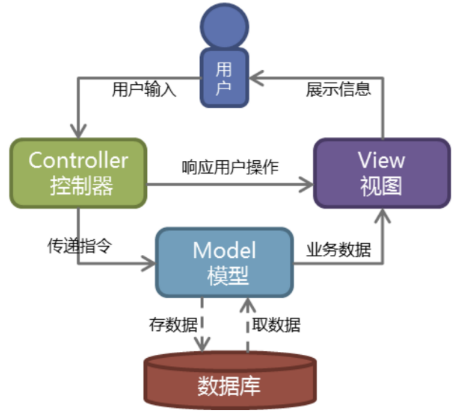
\includegraphics[width=0.4\textwidth]{part/互联/django/pic/概述/MVC模型示意图.png}
  \caption{MVC模型示意图}
  \label{fig:MVC模型示意图}
\end{figure}

\subsection{MTV模型}
Django 的 MTV 模式本质上和 MVC 是一样的，也是为了各组件间保持松耦合关系，只是定义上有些许不同，Django 的 MTV 分别是指：
\begin{enumerate}[label=\arabic*)]
  \item M 表示模型（Model）：编写程序应有的功能，负责业务对象与数据库的映射(ORM)。
  \item T 表示模板 (Template)：负责如何把页面(html)展示给用户。
  \item V 表示视图（View）：负责业务逻辑，并在适当时候调用 Model和 Template。
\end{enumerate}

除了以上三层之外，还需要一个 URL 分发器，它的作用是将一个个 URL 的页面请求分发给不同的 View 处理，View 再调用相应的 Model 和 Template。


\subsection{Django的工作流程}
\begin{figure}[htpb]
  \centering
  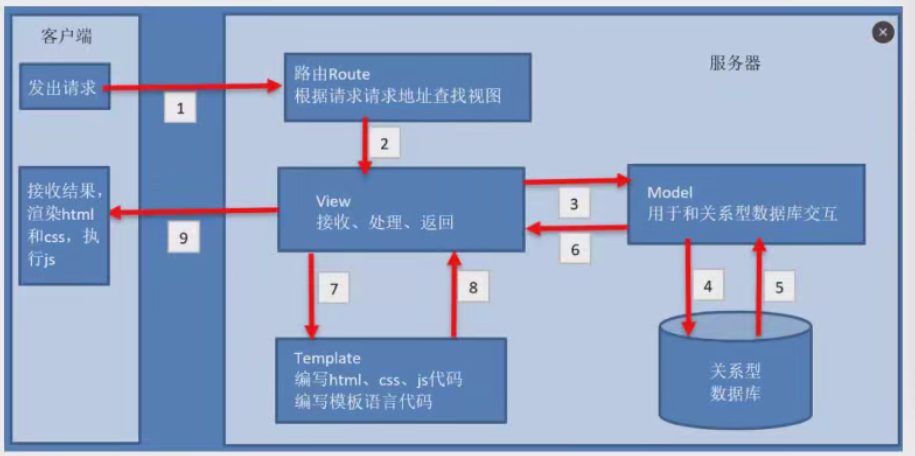
\includegraphics[width=0.4\textwidth]{part/互联/django/pic/概述/Django流程.png}
  \caption{Django流程}
  \label{fig:Django流程}
\end{figure}

\begin{enumerate}[label=\arabic*)]
  \item 浏览器通过域名发送一个 HTTP 请求到 Django 服务器。
  \item 路由(URLconf)接收到请求，网站的功能模块被映射到一个 URL(路由)。
  \item django根据请求的URL调用相应的视图函数(views)。
  \item 视图函数处理请求，可能会与数据库交互，然后返回一个 HTTP 响应。

  \begin{enumerate}[itemindent=1em,label=\arabic*)]
    \item 数据模型(Model)：与数据库交互，处理数据。
    \item 当数据模型获取到数据后，视图函数将数据传递给模板(template,存储前端的html文件)。
    \item 模板将数据渲染到前端页面。
  \end{enumerate}
  
  \item Django 将响应发送回浏览器，浏览器将其呈现给用户。
\end{enumerate}


\section{Django的安装}
\subsection{conda安装}
\begin{lstlisting}[style=demostyle,numbers=none]
$> conda create --name mydjango python=3.10
$> conda activate mydjango
$> conda install django==3.0.3
$ python3 -m django --version
3.0.3
\end{lstlisting}

\subsection{pip安装}
\begin{lstlisting}[style=demostyle,numbers=none]
$> sudo pip3 install Django -i https://pypi.tuna.tsinghua.edu.cn/simple
$> sudo pip3 install Django==3.0.6 -i https://pypi.tuna.tsinghua.edu.cn/simple
\end{lstlisting}



\section{主项目}
\subsection{创建项目}
\begin{lstlisting}[style=demostyle,numbers=none]
$> django-admin startproject recruitment_demo
$> tree
|-- manage.py # 命令行工具, 用于管理项目
`-- recruitment_demo # 项目的容器
    |-- __init__.py # 一个空文件，告诉 Python 该目录是一个 Python 包
    |-- __pycache__ # 编译后的文件
    │   |-- __init__.cpython-310.pyc
    │   |-- settings.cpython-310.pyc
    │   |-- urls.cpython-310.pyc
    │   `-- wsgi.cpython-310.pyc
    |-- asgi.py # 一个 ASGI 兼容的 Web 服务器入口点
    |-- settings.py # 项目的配置文件
    |-- urls.py # 项目的 URL 声明, 一份由 Django 驱动的网站"目录"
    `-- wsgi.py # 一个 WSGI 兼容的 Web 服务器的入口点
\end{lstlisting}
\subsection{查询帮助}
\begin{lstlisting}[style=demostyle,numbers=none]
$> python manage.py help
Type 'manage.py help <subcommand>' for help on a specific subcommand.

Available subcommands:

[auth]
    changepassword
    createsuperuser

[contenttypes]
    remove_stale_contenttypes

[django]
    check
    compilemessages
    createcachetable
    dbshell
    diffsettings
    dumpdata
    flush
    inspectdb
    loaddata
    makemessages
    makemigrations
    migrate
    sendtestemail
    shell
    showmigrations
    sqlflush
    sqlmigrate
    sqlsequencereset
    squashmigrations
    startapp
    startproject
    test
    testserver

[sessions]
    clearsessions

[staticfiles]
    collectstatic
    findstatic
    runserver
\end{lstlisting}

\begin{enumerate}[label=\arabic*)]
  \item auth：用户认证系统,与 Django 的认证系统（用户、权限、组等）相关
  \begin{enumerate}[itemindent=1em,label=\arabic*)]
    \item \codeinline{changepassword}：修改用户密码。
    \item \codeinline{createsuperuser}：创建超级用户。
  \end{enumerate}

  \item contenttypes：内容类型框架相关，内容类型框架允许你以统一的方式处理不同类型的模型。
  \begin{enumerate}[itemindent=1em,label=\arabic*)]
    \item \codeinline{remove\_stale\_contenttypes}：删除无用的内容类型。
  \end{enumerate}
  
  \item django：Django 管理命令,涉及数据库迁移、开发环境管理、数据导入导出等。
  \begin{enumerate}[itemindent=1em,label=\arabic*)]
    \item \codeinline{check}：检查 Django 项目中是否存在任何错误或潜在问题。适用于快速检测项目状态。
    \item \codeinline{compilemessages}：编译 Django 项目中的翻译文件（.po 文件转 .mo 文件）。用于多语言支持。
    \item \codeinline{createcachetable}：创建数据库表以便使用缓存系统。用于缓存的数据库存储。
    \item \codeinline{dbshell}：打开一个数据库 shell（命令行界面），可以直接操作项目的数据库。
    \item \codeinline{diffsettings}：显示当前项目配置与默认配置的差异，帮助你查看哪些设置被修改过。
    \item \codeinline{dumpdata}：将数据库中的数据导出为 JSON 格式，通常用于备份或者数据迁移。
    \item \codeinline{flush}：重置数据库，将所有的数据清除并恢复到初始状态。会清空所有表，通常用于开发时清理数据。
    \item \codeinline{inspectdb}：根据现有的数据库表生成对应的 Django 模型代码（即反向生成模型）。
    \item \codeinline{loaddata}：加载之前导出的数据文件（通常是 JSON 格式）到数据库中。
    \item \codeinline{makemessages}：扫描代码，查找需要翻译的字符串，并生成相应的翻译文件（.po）。
    \item \codeinline{makemigrations}：生成数据库迁移文件，记录模型的更改。迁移是 Django 对数据库结构变化的管理。
    \item \codeinline{migrate}：应用迁移文件，更新数据库结构，使其与当前的模型状态一致。
    \item \codeinline{sendtestemail}：发送一个测试电子邮件，用于测试邮件设置是否正常。
    \item \codeinline{shel}l：启动 Django 的交互式 Python shell，允许你直接在命令行中操作 Django 项目，例如查询数据库、操作模型等。
    \item \codeinline{showmigrations}：显示当前数据库迁移的状态，哪些迁移已应用，哪些没有应用。
    \item \codeinline{sqlflush}：生成并显示清空数据库表（flush）所需要的 SQL 语句。
    \item \codeinline{sqlmigrate}：查看某个迁移文件对应的 SQL 语句。
    \item \codeinline{sqlsequencereset}：查看重置数据库表的序列（主要是用于自增字段）所需要的 SQL 语句。
    \item \codeinline{squashmigrations}：将多个迁移合并为一个迁移文件，帮助减少迁移文件的数量。
    \item \codeinline{startapp}：创建一个新的 Django 应用，并生成默认的目录结构。
    \item \codeinline{startproject}：创建一个新的 Django 项目，初始化基本的项目结构。
    \item \codeinline{test}：运行 Django 测试框架中的测试，通常用于验证你的代码是否正常工作。
    \item \codeinline{testserver}：启动一个测试服务器，用于测试环境中的调试和运行。
  \end{enumerate}
  

  
\end{enumerate}



\subsection{启动项目}
\begin{lstlisting}[style=demostyle,numbers=none]
$> python manage.py runserver ip地址:端口

# 本地访问
$> python manage.py runserver 0.0.0.0:8000
\end{lstlisting}

然后访问\codeinline{http://localhost:8000/}，可以看到如图\ref{fig:Django启动成功}所示的页面。
\begin{figure}[htpb]
  \centering
  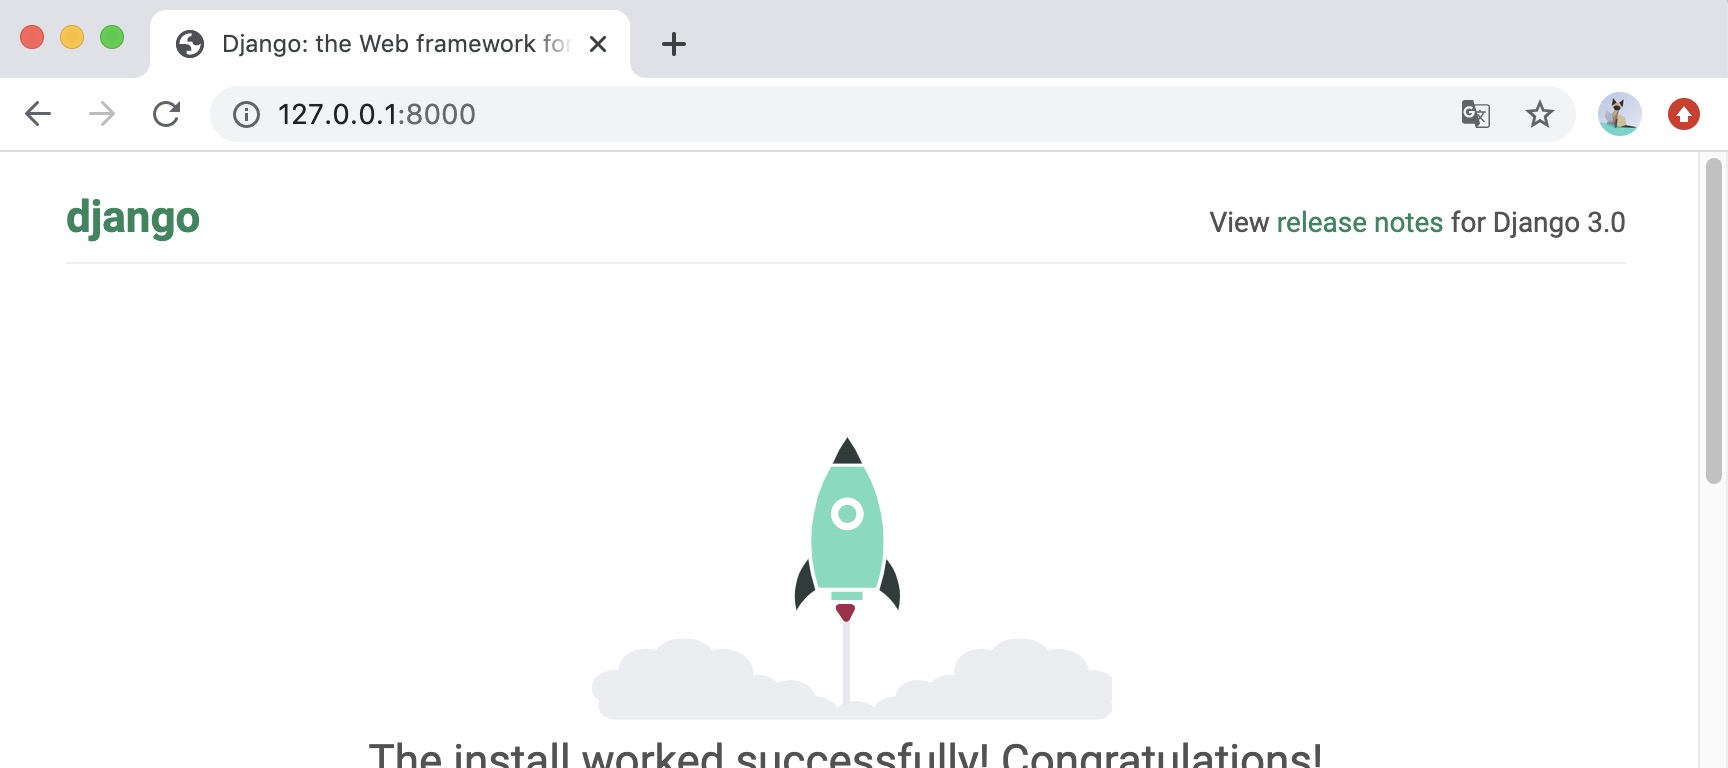
\includegraphics[width=0.4\textwidth]{part/互联/django/pic/概述/Django启动成功.png}
  \caption{Django启动成功}
  \label{fig:Django启动成功}
\end{figure}



\section{创建子应用}
\subsubsection{子应用的作用}
\begin{example}
  \exProblem
  Django的主项目相当一家公司，公司下面有很多部门：开发部、运营部、财务部等等。
  
  \begin{enumerate}[label=\arabic*)]
    \item 公司->主项目
    \item 部门->子应用
  \end{enumerate}
  
  每个子应用之间相互独立，可以单独运行，也可以被其他项目引用。
\end{example}

\subsection{创建子应用}
\begin{lstlisting}[style=demostyle,numbers=none]
$> python manage.py startapp 子应用名称
\end{lstlisting}

\begin{lstlisting}[style=demostyle,numbers=none]
$> python manage.py startapp jobs
$> tree
|-- manage.py
|-- recruitment_demo # 主项目的容器
│   |-- __init__.py
...
`-- jobs  # 子应用的文件夹
    |-- __init__.py
    |-- admin.py  # 管理后台
    |-- apps.py   # 子应用的配置文件
    |-- migrations # 数据库迁移文件
    │   `-- __init__.py
    |-- models.py
    |-- tests.py   # 单元测试
    `-- views.py   # 视图函数
\end{lstlisting}

\subsection{注册子应用}
在主项目的\codeinline{settings.py}文件中注册子应用。
\begin{lstlisting}[style=demostyle,numbers=none]
$> ls 
jobs  recruitment_demo  
$> cat recruitment_demo/settings.py # recruitment_demo是主项目的文件夹名称  
INSTALLED_APPS = [
    'django.contrib.admin',
    'django.contrib.auth',
    'django.contrib.contenttypes',
    'django.contrib.sessions',
    'django.contrib.messages',
    'django.contrib.staticfiles',
    'jobs',  # 注册子应用, jobs是子应用的文件夹名称
    # 或者
    'job.apps.JobConfig',  # 注册子应用, job是子应用的文件夹名称
]
\end{lstlisting}

在注册子应用有两种写法
\begin{enumerate}[label=\arabic*)]
  \item \codeinline{'子模块名'}

  这种写法会自动加载子应用的配置文件\codeinline{apps.py}，并执行其中的代码。

  \item \codeinline{'子模块名.apps.子模块名Config'}

  这个\codeinline{子模块名Config}是\codeinline{apps.py}中个一个类，一般约定的写法。

  该方法显式指定应用的配置入口，Django 会加载该配置，而不是使用默认配置。
  可以在\codeinline{子模块名Config}中定义一些特定的行为
\begin{lstlisting}[style=demostyle,numbers=none]
class BaseInfoConfig(AppConfig):
    default_auto_field = 'django.db.models.BigAutoField' # 指定模型的主键类型为大整型
    name = 'base_info' # 指定应用的名称，就是startapp时的应用名称
    verbose_name = '基础信息' # 指定应用的中文名称, 在admin后台显示
\end{lstlisting}    

\end{enumerate}



% \subsection{创建数据库}
% \begin{lstlisting}[style=demostyle,numbers=none]
% # 1.makemigrations 会生成一个文件，里面存储的是关于数据库的一些操作    
% $ python manage.py makemigrations
% Migrations for 'jobs':
%   jobs/migrations/0001_initial.py
%     - Create model Job

% # 2.migrate 会根据makemigrations生成的文件，去执行数据库操作
% $> python manage.py migrate   
% Operations to perform:
%   Apply all migrations: admin, auth, contenttypes, jobs, sessions
% Running migrations:
%   Applying jobs.0001_initial... OK 
% \end{lstlisting}    















\chapter{Django模型(数据库)}

\section{Django模型简介}
Django 对各种数据库提供了很好的支持，包括：PostgreSQL、MySQL、SQLite、Oracle。

Django 为这些数据库提供了统一的调用API。 我们可以根据自己业务需求选择不同的数据库。


\section{数据库的配置}
\subsection{sqlite3数据库配置}
Django 默认使用的是sqlite3数据库，不需要配置，也不需要安装额外的数据库驱动。
\subsubsection{settings.py配置}
\begin{lstlisting}[style=demostyle,numbers=none]
$> cd 主项目目录
$> cat settings.py
DATABASES = {
    'default': {
        'ENGINE': 'django.db.backends.sqlite3',
        'NAME': os.path.join(BASE_DIR, 'db.sqlite3'),
    }
}
\end{lstlisting}    

\subsection{MySQL数据库配置}
\subsubsection{安装MySQL驱动}
\begin{lstlisting}[style=demostyle,numbers=none]
$> sudo pip3 install pymysql
$> conda install pymysql
\end{lstlisting}

如果使用\codeinline{pymysql}需要在 \textcolor{YBXPurple}{主项目}的\codeinline{\_\_init\_\_.py}文件中添加如下代码：
\begin{lstlisting}[style=demostyle,numbers=none]
import pymysql
pymysql.install_as_MySQLdb()
\end{lstlisting}    

\subsubsection{提前配置数据库}
\textcolor{red}{\textbf{ORM 无法操作到数据库级别，只能操作到数据表}}
\begin{enumerate}[label=\arabic*)]
    \item 创建一个新数据库
\begin{lstlisting}[style=demostyle,numbers=none]
$> mysql -u root -p
mysql> create database 数据库名称 default charset=utf8; # 防止编码问题，指定为 utf8
\end{lstlisting}

    \item 创建一个新用户, 并授权(刷新权限)
\begin{lstlisting}[style=demostyle,numbers=none]
mysql> create user '用户名'@'主机名' identified by '密码'; # 主机名可以是 localhost
mysql> grant all privileges on 数据库名.* to '用户名'@'主机名'; # 授权
mysql> flush privileges; # 刷新权限
\end{lstlisting}

\end{enumerate}

\begin{example}
    \exProblem
    创建一个数据库\codeinline{django\_db}，用户名\codeinline{django\_user}，密码\codeinline{your\_password}，并授权\codeinline{django\_user}可以访问\codeinline{django\_db}数据库。
    \exSolution
\begin{lstlisting}[style=demostyle,numbers=none]
mysql> # 创建数据库    
mysql> CREATE DATABASE django_db DEFAULT CHARACTER SET utf8; 
Query OK, 1 row affected (0.03 sec)

mysql> # 创建用户
mysql> CREATE USER 'django_user'@'%' IDENTIFIED BY 'your_password';
Query OK, 1 row affected (0.03 sec)

mysql> # 授予 django_user，使其可以访问 django_db 数据库：
mysql> GRANT ALL PRIVILEGES ON django_db.* TO 'django_user'@'%';
Query OK, 0 rows affected (0.01 sec)

mysql> # 刷新权限
mysql> flush privileges;
Query OK, 0 rows affected (0.01 sec)
\end{lstlisting}
\end{example}


\subsubsection{配置settings.py}
\begin{lstlisting}[style=demostyle,numbers=none]
$> cat settings.py    
DATABASES = {
    'default': {
        'ENGINE': 'django.db.backends.mysql',
        'NAME': '数据库名称',
        'USER': '数据库用户名',
        'PASSWORD': '数据库密码',
        'HOST': '数据库地址',
        'PORT': '数据库端口',
    }
}
\end{lstlisting}


\begin{example}
    \exProblem
    配置MySQL数据库
    \exSolution
\begin{lstlisting}[style=demostyle,numbers=none]
$> cat settings.py    
DATABASES = {
    'default': {
        # 使用 MySQL 引擎
        'ENGINE': 'django.db.backends.mysql',  
        # 数据库名称，修改为你在 MySQL 中创建的数据库名
        'NAME': 'django_db',                   
        # 在 MySQL 中创建的用户名
        'USER': 'django_user',                 
        # 该用户的密码
        'PASSWORD': 'your_password',           
        # 如果 MySQL 在本地机器上，使用 localhost，或者是容器 IP
        'HOST': 'localhost',                   
        # MySQL 端口
        'PORT': '3306',                        
    }
}

# 运行数据库迁移
$> python manage.py migrate
Operations to perform:
  Apply all migrations: TestModel, admin, auth, contenttypes, jobs, sessions
Running migrations:
  Applying TestModel.0001_initial... OK
  Applying TestModel.0002_auto_20241114_0739... OK
  Applying TestModel.0003_auto_20241114_0804... OK
  Applying contenttypes.0001_initial... OK
  Applying auth.0001_initial... OK
  Applying admin.0001_initial... OK
  Applying admin.0002_logentry_remove_auto_add... OK
  Applying admin.0003_logentry_add_action_flag_choices... OK
  Applying contenttypes.0002_remove_content_type_name... OK
  Applying auth.0002_alter_permission_name_max_length... OK
  Applying auth.0003_alter_user_email_max_length... OK
  Applying auth.0004_alter_user_username_opts... OK
  Applying auth.0005_alter_user_last_login_null... OK
  Applying auth.0006_require_contenttypes_0002... OK
  Applying auth.0007_alter_validators_add_error_messages... OK
  Applying auth.0008_alter_user_username_max_length... OK
  Applying auth.0009_alter_user_last_name_max_length... OK
  Applying auth.0010_alter_group_name_max_length... OK
  Applying auth.0011_update_proxy_permissions... OK
  Applying jobs.0001_initial... OK
  Applying sessions.0001_initial... OK


# 查看数据库
$> docker start mysql57
$> docker exec -it mysql57 mysql -u root -p
Enter password:
mysql> show databases;
+--------------------+
| Database           |
+--------------------+
| information_schema |
| django_db          |
| mysql              |
| performance_schema |
| sys                |
| testdb             |
| testdb1            |
+--------------------+
7 rows in set (0.00 sec)

mysql> USE django_db;
Reading table information for completion of table and column names
You can turn off this feature to get a quicker startup with -A

Database changed
mysql> SHOW TABLES;
+----------------------------+
| Tables_in_django_db        |
+----------------------------+
| auth_group                 |
| auth_group_permissions     |
| auth_permission            |
| auth_user                  |
| auth_user_groups           |
| auth_user_user_permissions |
| django_admin_log           |
| django_content_type        |
| django_migrations          |
| django_session             |
| jobs                       |
| jobs_job                   |
| people                     |
+----------------------------+
13 rows in set (0.00 sec)

mysql>
\end{lstlisting}
\end{example}

\subsection{PostgreSQL数据库配置}
\subsubsection{安装psycopg2}
\begin{lstlisting}[style=demostyle,numbers=none]
$> sudo sh -c 'echo "deb http://apt.postgresql.org/pub/repos/apt $(lsb_release -cs)-pgdg main" > /etc/apt/sources.list.d/pgdg.list'
$> wget --quiet -O - https://www.postgresql.org/media/keys/ACCC4CF8.asc | sudo apt-key add -
$> sudo apt update
$> sudo apt install postgresql-server-dev-9.6
$> pg_config --version
PostgreSQL 9.6.24
$> pip install psycopg2==2.8.6 # 因为是Django3.X，所以安装2.8.6版本
\end{lstlisting}

或者安装预编译的二进制文件psycopg2-binary
\begin{lstlisting}[style=demostyle,numbers=none]
$> pip install psycopg2-binary
\end{lstlisting}

\subsubsection{[可选]配置 PostgreSQL 的远程访问}
默认情况下，PostgreSQL 仅允许本地访问。如果需要从其他容器或主机访问数据库，修改以下配置：
\begin{enumerate}[label=\arabic*)]
    \item 拷贝文件进行修改

\begin{lstlisting}[style=demostyle,numbers=none]
$> docker ps 
CONTAINER ID   IMAGE          COMMAND         NAMES
fcca6d8e3b95   postgres:9.6   "docker-ent…"   postgres96

$> docker exec postgres96 cp /var/lib/postgresql/data/pg_hba.conf /var/lib/postgresql/data/pg_hba.conf.bak
$> docker cp postgres96:/var/lib/postgresql/data/pg_hba.conf ./pg_hba.conf
$> vim pg_hba.conf
# 添加下面内容
host    django_db    django_user    0.0.0.0/0    md5

$> # 其中 host表示允许通过 TCP/IP 协议进行远程访问，而不是本地 Unix 套接字连接(local)。
$> # django_db 是数据库名称，django_user 是数据库用户名，
$> # 0.0.0.0/0 表示允许从任何 IP 地址访问。
$> # md5 表示使用 md5 加密方式验证密码。

$> docker cp ./pg_hba.conf postgres96:/var/lib/postgresql/data/pg_hba.conf
$> docker restart postgres96
\end{lstlisting}

    \item 直接\codeinline{echo}修改
\begin{lstlisting}[style=demostyle,numbers=none]
$> docker exec postgres96 cp /var/lib/postgresql/data/pg_hba.conf /var/lib/postgresql/data/pg_hba.conf.bak
$> docker exec postgres96 bash -c "echo 'host    django_db    django_user    0.0.0.0/0    md5' >> /var/lib/postgresql/data/pg_hba.conf"
$> docker restart postgres96
\end{lstlisting}        
\end{enumerate}

测试连接
\begin{lstlisting}[style=demostyle,numbers=none]
$> docker exec -it postgres96 psql -h localhost -U django_user -d django_db
\end{lstlisting}


\subsubsection{配置settings.py}
\begin{lstlisting}[style=demostyle,numbers=none]
$> cat settings.py    
DATABASES = {
    'default': {
        'ENGINE': 'django.db.backends.postgresql',
        'NAME': 'your_db',          # 数据库名称（默认为 postgres）
        'USER': 'your_user',        # 数据库用户（默认为 postgres）
        'PASSWORD': 'your_password',# 数据库密码
        'HOST': 'localhost',        # 主机地址
        'PORT': '5432',             # 端口号
    }
}
\end{lstlisting}

\begin{example}
    \exProblem
    创建一个数据库\codeinline{django\_db}，用户名\codeinline{django\_user}，密码\codeinline{django\_password}，
    并授权\codeinline{django\_user}可以访问\codeinline{django\_db}数据库。

    \exSolution
\begin{lstlisting}[style=demostyle,numbers=none]
$> $ docker exec -it postgres96 psql -U postgres
psql (9.6.24)
Type "help" for help.

postgres=# CREATE USER django_user WITH PASSWORD 'django_passwd';
CREATE ROLE

postgres=# CREATE DATABASE django_db OWNER django_user;
CREATE DATABASE

postgres=# GRANT ALL PRIVILEGES ON DATABASE django_db TO django_user;
GRANT
\end{lstlisting}

\begin{lstlisting}[style=demostyle,numbers=none]
$> docker restart postgres96
\end{lstlisting}

\begin{lstlisting}[style=demostyle,numbers=none]
$> cat settings.py
DATABASES = {
    'default': {
        'ENGINE': 'django.db.backends.postgresql',
        'NAME': 'django_db',          # 数据库名称
        'USER': 'django_user',        # 数据库用户名
        'PASSWORD': 'django_passwd',  # 数据库密码
        'HOST': 'localhost',          # 数据库主机
        'PORT': '5432',               # 数据库端口
    }
}
\end{lstlisting}    

运行数据库迁移
\begin{lstlisting}[style=demostyle,numbers=none]
$> python manage.py makemigrations
$> python manage.py migrate
\end{lstlisting}



    
\end{example}


\subsection{Redis数据库配置}

\section{定义模型}
\subsection{前提准备————创建子应用}
Django 规定，如果要使用模型，必须要创建一个子应用app。
\begin{lstlisting}[style=demostyle,numbers=none]
$> python manage.py startapp APP名
# 或者
$> django-admin startapp APP名
\end{lstlisting}

创建好了子应用后，会在项目目录下生成一个子应用目录，目录结构如下：
\begin{lstlisting}[style=demostyle,numbers=none]
$> django-admin startapp TestModel
$> $ tree TestModel/
TestModel/
|-- admin.py # 管理后台,
|-- apps.py # 应用配置
|-- __init__.py # 一个空文件，告诉 Python 该目录是一个 Python 包
|-- migrations  # 数据库迁移文件
│   `-- __init__.py
|-- models.py   # 模型文件
|-- tests.py    # 测试文件
`-- views.py    # 视图文件
\end{lstlisting}

\subsection{定义表结构}
\begin{enumerate}[label=\arabic*)]
    \item Django 的模型类必须继承自 \codeinline{django.db.models.Model} 类。

    \codeinline{models.Model} 是 Django 中定义模型类的基类，它包含了一些基本的属性和方法，用于定义数据库表的结构。

    \item 要在 \textcolor{YBXPurple}{子应用} 目录下的 \codeinline{models.py} 文件中定义模型类。
\end{enumerate}


\begin{lstlisting}[style=demostyle,numbers=none]
$> cat TestModel/models.py
from django.db import models # 导入模型类
 
"""
1.类名 People 表示数据库表名 
2.类属性 name 表示数据库表的字段名
  类属性 age 表示数据库表的字段名
3.类属性的值表示字段的类型
  CharField: 字符串类型 varchar
  IntegerField: 整数类型 int  
  max_length: 字符串类型的长度
"""
class People(models.Model):
    # id 在 Django 中会自动生成，不需要定义
    # id = models.AutoField(primary_key=True)
    name = models.CharField(max_length=20) # 相当于 varchar(20)
    age = models.IntegerField()
    gender = models.BooleanField(default=True)    
    # 外键关联，当关联的数据被删除时，本表中的数据也会被删除
    marjor = models.ForeignKey('Jobs', on_delete=models.CASCADE)

class Jobs(models.Model):
    job_name = models.CharField(max_length=20)
    job_salary = models.IntegerField()
    job_desc = models.TextField()
    job_address = models.CharField(max_length=50)
    
\end{lstlisting}

\subsubsection{ORM的字段类型}
在ORM的类属性中，与SQL的数据类型对应关系如下：
\begin{enumerate}[label=\arabic*)]
    \item \codeinline{models.CharField}：字符串类型 \codeinline{varchar}
    \item \codeinline{models.IntegerField}：整数类型 \codeinline{int}
    \item \codeinline{models.FloatField}：浮点类型 \codeinline{float}
    \item \codeinline{models.DateTimeField}：日期时间类型 \codeinline{datetime}
    \item \codeinline{models.BooleanField}：布尔类型 \codeinline{bool}
    \item \codeinline{models.AutoField}：自增长整数类型 \codeinline{int}（自动生成并递增）
    \item \codeinline{models.DecimalField}：高精度小数类型 \codeinline{decimal}
    \item \codeinline{models.TextField}：长文本类型 \codeinline{text}
    \item \codeinline{models.DateField}：日期类型 \codeinline{date}
    \item \codeinline{models.TimeField}：时间类型 \codeinline{time}
    \item \codeinline{models.EmailField}：电子邮件类型 \codeinline{varchar}（特定长度）
    \item \codeinline{models.URLField}：URL类型 \codeinline{varchar}（特定长度）
    \item \codeinline{models.FileField}：文件类型 \codeinline{blob} 或 \codeinline{varchar}（用于文件路径）
    \item \codeinline{models.ImageField}：图像类型 \codeinline{blob} 或 \codeinline{varchar}（用于图像路径）
    \item \codeinline{models.JSONField}：JSON类型 \codeinline{json}（在一些数据库中）
    \item \codeinline{models.UUIDField}：UUID类型 \codeinline{uuid}
    \item \codeinline{models.ForeignKey}：外键关系 \codeinline{int}（指向另一表的主键）
    \item \codeinline{models.ManyToManyField}：多对多关系（通过连接表实现）
    \item \codeinline{models.OneToOneField}：一对一关系 \codeinline{int}（指向另一表的主键）
\end{enumerate}

\subsubsection{外键关联}
\begin{lstlisting}[style=demostyle,numbers=none]
models.ForeignKey('关联的表名', on_delete=models.CASCADE)
# on_delete=models.CASCADE 表示当关联的数据被删除时，本表中的数据也会被删除
\end{lstlisting}

\subsection{添加INSTALLED\_APPS}
在主项目的\codeinline{settings.py}文件中，设置\codeinline{INSTALLED\_APPS}，添加创建的app。
\begin{lstlisting}[style=demostyle,numbers=none]
$> tree
.
|-- HelloWorld
│   |-- __init__.py
│   |-- settings.py
....
|-- TestModel
│   |-- models.py
....

$> cat HelloWorld/settings.py
INSTALLED_APPS = [
    'django.contrib.admin',
    'django.contrib.auth',
    'django.contrib.contenttypes',
    'django.contrib.sessions',
    'django.contrib.messages',
    'django.contrib.staticfiles',
    'TestModel', # 添加创建的 app
]
\end{lstlisting}

\subsection{生成迁移文件}
\textcolor{blue}{\textbf{迁移}}(Migration)是 Django 中的一个重要概念，
用于将模型的修改(在文件\codeinline{models.py})同步到数据库中。

\begin{enumerate}[label=\arabic*)]
    \item \codeinline{makemigrations}：根据\textcolor{YBXPurple}{主项目}中的\codeinline{settings.py}文件中的\codeinline{INSTALLED\_APPS}，生成迁移文件
    \item \codeinline{migrate}：执行迁移文件
\end{enumerate}

\begin{lstlisting}[style=demostyle,numbers=none]
$ python3 manage.py migrate   # 创建表结构
$ python3 manage.py makemigrations TestModel  # 让 Django 知道我们在我们的模型有一些变更
$ python3 manage.py migrate TestModel   # 创建表结构
\end{lstlisting}

\begin{lstlisting}[style=demostyle,numbers=none]
$> python3 manage.py migrate   # 创建表结构
Operations to perform:
  Apply all migrations: admin, auth, contenttypes, jobs, sessions
Running migrations:
  No migrations to apply.
  Your models have changes that are not yet reflected in a migration, and so won't be applied.
  Run 'manage.py makemigrations' to make new migrations, and then re-run 'manage.py migrate' to apply them.
$> python3 manage.py makemigrations TestModel
Migrations for 'TestModel':
  TestModel/migrations/0001_initial.py
    - Create model Test

$> python3 manage.py migrate   # 创建表结构
Operations to perform:
  Apply all migrations: TestModel, admin, auth, contenttypes, jobs, sessions
Running migrations:
  Applying TestModel.0001_initial... OK
\end{lstlisting}  

如果迁移失败可以，删除迁移文件，重新迁移
\begin{lstlisting}[style=demostyle,numbers=none]
$> find . -path "*/migrations/*.py" -not -name "__init__.py" -delete
$> find . -path "*/migrations/*.pyc"  -delete
\end{lstlisting}

\subsubsection{查看数据库}
\begin{lstlisting}[style=demostyle,numbers=none]
$> python manage.py dbshell # 不同的数据库，命令不同
sqlite> .tables
auth_user                auth_user_user_permissions
auth_user_groups         django_admin_log
auth_group               django_content_type
auth_group_permissions   django_migrations
auth_permission          django_session
TestModel_People
TestModel_Jobs

sqlite> PRAGMA table_info(TestModel_People);
0|id|integer|1||1
1|name|varchar(20)|1||0
2|age|integer|1||0
3|gender|bool|1||0
4|marjor_id|integer|1||0

sqlite> PRAGMA table_info(TestModel_Jobs);
0|id|integer|1||1
1|job_name|varchar(20)|1||0
2|job_salary|integer|1||0
3|job_desc|text|1||0
4|job_address|varchar(50)|1||0
\end{lstlisting}          


\subsection{常见报错}
\textcolor{red}{\textbf{注意}}：如果没有在\codeinline{INSTALLED\_APPS}中添加创建的app，会出现如下错误：

\begin{lstlisting}[style=demostyle,numbers=none]
$ python3 manage.py migrate   # 创建表结构
Operations to perform:
  Apply all migrations: admin, auth, contenttypes, jobs, sessions
Running migrations:
  No migrations to apply.
  Your models have changes that are not yet reflected in a migration, and so won't be applied.
  Run 'manage.py makemigrations' to make new migrations, and then re-run 'manage.py migrate' to apply them.

$> python3 manage.py makemigrations TestModel
No installed app with label 'TestModel'.

$> python3 manage.py migrate TestModel
CommandError: No installed app with label 'TestModel'.  
\end{lstlisting}

\subsubsection{mysqlclient报错}
\begin{lstlisting}[style=demostyle,numbers=none]
$> python3 manage.py migrate
File "/usr/local/lib/python3.6/dist-packages/django/db/backends/mysql/base.py", line 36, in <module>
    raise ImproperlyConfigured('mysqlclient 1.3.13 or newer is required; you have %s.' % Database.__version__)
django.core.exceptions.ImproperlyConfigured: mysqlclient 1.3.13 or newer is required; you have 0.9.3.
\end{lstlisting}


MySQLclient 目前只支持到 Python3.4，因此如果使用的更高版本的 python

需要修改如下：通过报错信息的文件路径找到
\begin{lstlisting}[style=demostyle,numbers=none]
$> vim /usr/local/lib/python3.6/dist-packages/django/db/backends/mysql/base.py
# 把这两行代码注释掉
if version < (1, 3, 13):
    raise ImproperlyConfigured('mysqlclient 1.3.13 or newer is required; you have %s.' % Database.__version__)
\end{lstlisting}


\section{对象关系映射(ORM)}
Django 模型使用自带的 ORM。

\textcolor{blue}{\textbf{对象关系映射}}（Object Relational Mapping，简称 ORM ）用于实现面向对象编程语言里不同类型系统的数据之间的转换。

\subsection{ORM与数据库的对应关系}
\begin{enumerate}[label=\arabic*)]
    \item Models类：数据库表
    \item Models类的属性：数据库表的字段
    \item Models类的方法：数据库表的操作
    \item Models类的方法与数据库的操作：数据库表的增删改查
    \item 对象实例：数据库表的记录
\end{enumerate}

\subsection{数据库操作}
\subsubsection{增}

增加数据一般使用\codeinline{save()}方法。

在app的\codeinline{views.py}文件中添加代码。
\begin{lstlisting}[style=demostyle,numbers=none]
$> cat TestModel/views.py
from django.shortcuts import render
from django.http import HttpResponse
from .models import Test

def insert(request):
    test1 = Test(name='ZJW', age=18)
    test1.save()
    return HttpResponse("<p>数据添加成功！</p>")
\end{lstlisting}

\subsubsection{查询}

\begin{enumerate}
    \item \codeinline{all()}：获取全部数据
    \item \codeinline{filter()}：根据条件过滤数据
    \item \codeinline{get()}：根据条件获取单个对象
    \item \codeinline{order\_by()}：根据字段排序
\end{enumerate}

在app的\codeinline{views.py}文件中添加代码。
\begin{lstlisting}[style=demostyle,numbers=none]
$> cat TestModel/views.py
from django.shortcuts import render
from django.http import HttpResponse
from .models import Test

def select(request):
    # 初始化
    response = ""
    response1 = ""


    # 通过objects这个模型管理器的all()获得所有数据行，相当于SQL中的SELECT * FROM
    listTest = Test.objects.all()
        
    # filter相当于SQL中的WHERE，可设置条件过滤结果
    response2 = Test.objects.filter(id=1) 

    # 获取单个对象
    response3 = Test.objects.get(id=1) 

    # 限制返回的数据 相当于 SQL 中的 OFFSET 0 LIMIT 2;
    Test.objects.order_by('name')[0:2]

    #数据排序
    Test.objects.order_by("id")

    # 上面的方法可以连锁使用
    Test.objects.filter(name="runoob").order_by("id")

    # 输出所有数据
    for var in listTest:
        response1 += var.name + " "
    response = response1
    return HttpResponse("<p>" + response + "</p>")
\end{lstlisting}

\subsubsection{改}
修改数据可以使用\codeinline{save()}或\codeinline{update()}方法。

在app的\codeinline{views.py}文件中添加代码。
\begin{lstlisting}[style=demostyle,numbers=none]
$> cat TestModel/views.py
from django.shortcuts import render
from django.http import HttpResponse
from .models import Test

def update(request):
    # 修改其中一个id=1的name字段，再save
    test1 = Test.objects.get(id=1)
    test1.name = 'Google'
    test1.save()

    # 另外一种方式
    Test.objects.filter(id=1).update(name='Google')

    # 修改所有的列
    Test.objects.all().update(name='Google')

    return HttpResponse("<p>修改成功</p>")
\end{lstlisting}

\subsubsection{删}
删除数据可以使用\codeinline{delete()}方法。

在app的\codeinline{views.py}文件中添加代码。
\begin{lstlisting}[style=demostyle,numbers=none]
$> cat TestModel/views.py
from django.shortcuts import render
from django.http import HttpResponse
from .models import Test

def delete(request):
    # 删除id=1的数据
    test1 = Test.objects.get(id=1)
    test1.delete()

    # 另外一种方式
    Test.objects.filter(id=1).delete()

    # 删除所有数据
    # Test.objects.all().delete()

    return HttpResponse("<p>删除成功</p>")
\end{lstlisting}




\section{后台管理}
\subsection{创建超级用户}
\begin{lstlisting}[style=demostyle,numbers=none]
$> django-admin startproject mysite
$> cd mysite
$> python manage.py createsuperuser
Username (leave blank to use 'admin'): admin
Email address: admin@example.com
Password:
Password (again):
\end{lstlisting}

访问\codeinline{http://127.0.0.1:8000/admin/}

\subsection{设置中文}
在主项目的\codeinline{settings.py}文件中设置中文。
\begin{lstlisting}[style=demostyle,numbers=none]
$> cat mysite/settings.py
LANGUAGE_CODE = 'en-us'
# LANGUAGE_CODE = 'zh-hans'  # 设置中文
\end{lstlisting}  

\subsection{注册模型}
将子应用的模型在后台管理页面也可以看到，需要在子应用的\codeinline{admin.py}文件中注册模型。
\begin{lstlisting}[style=demostyle,numbers=none]
$> cat TestModel/models.py
...
class People(models.Model):
...
class Jobs(models.Model):
...


$> cat TestModel/admin.py
from django.contrib import admin # 导入admin模块
from TestModel.models import People, Jobs # 导入模型类


# Register your models here.
admin.site.register(People) # 注册模型类
admin.site.register(Jobs) # 注册模型类
\end{lstlisting}

\begin{figure}[htpb]
    \centering
    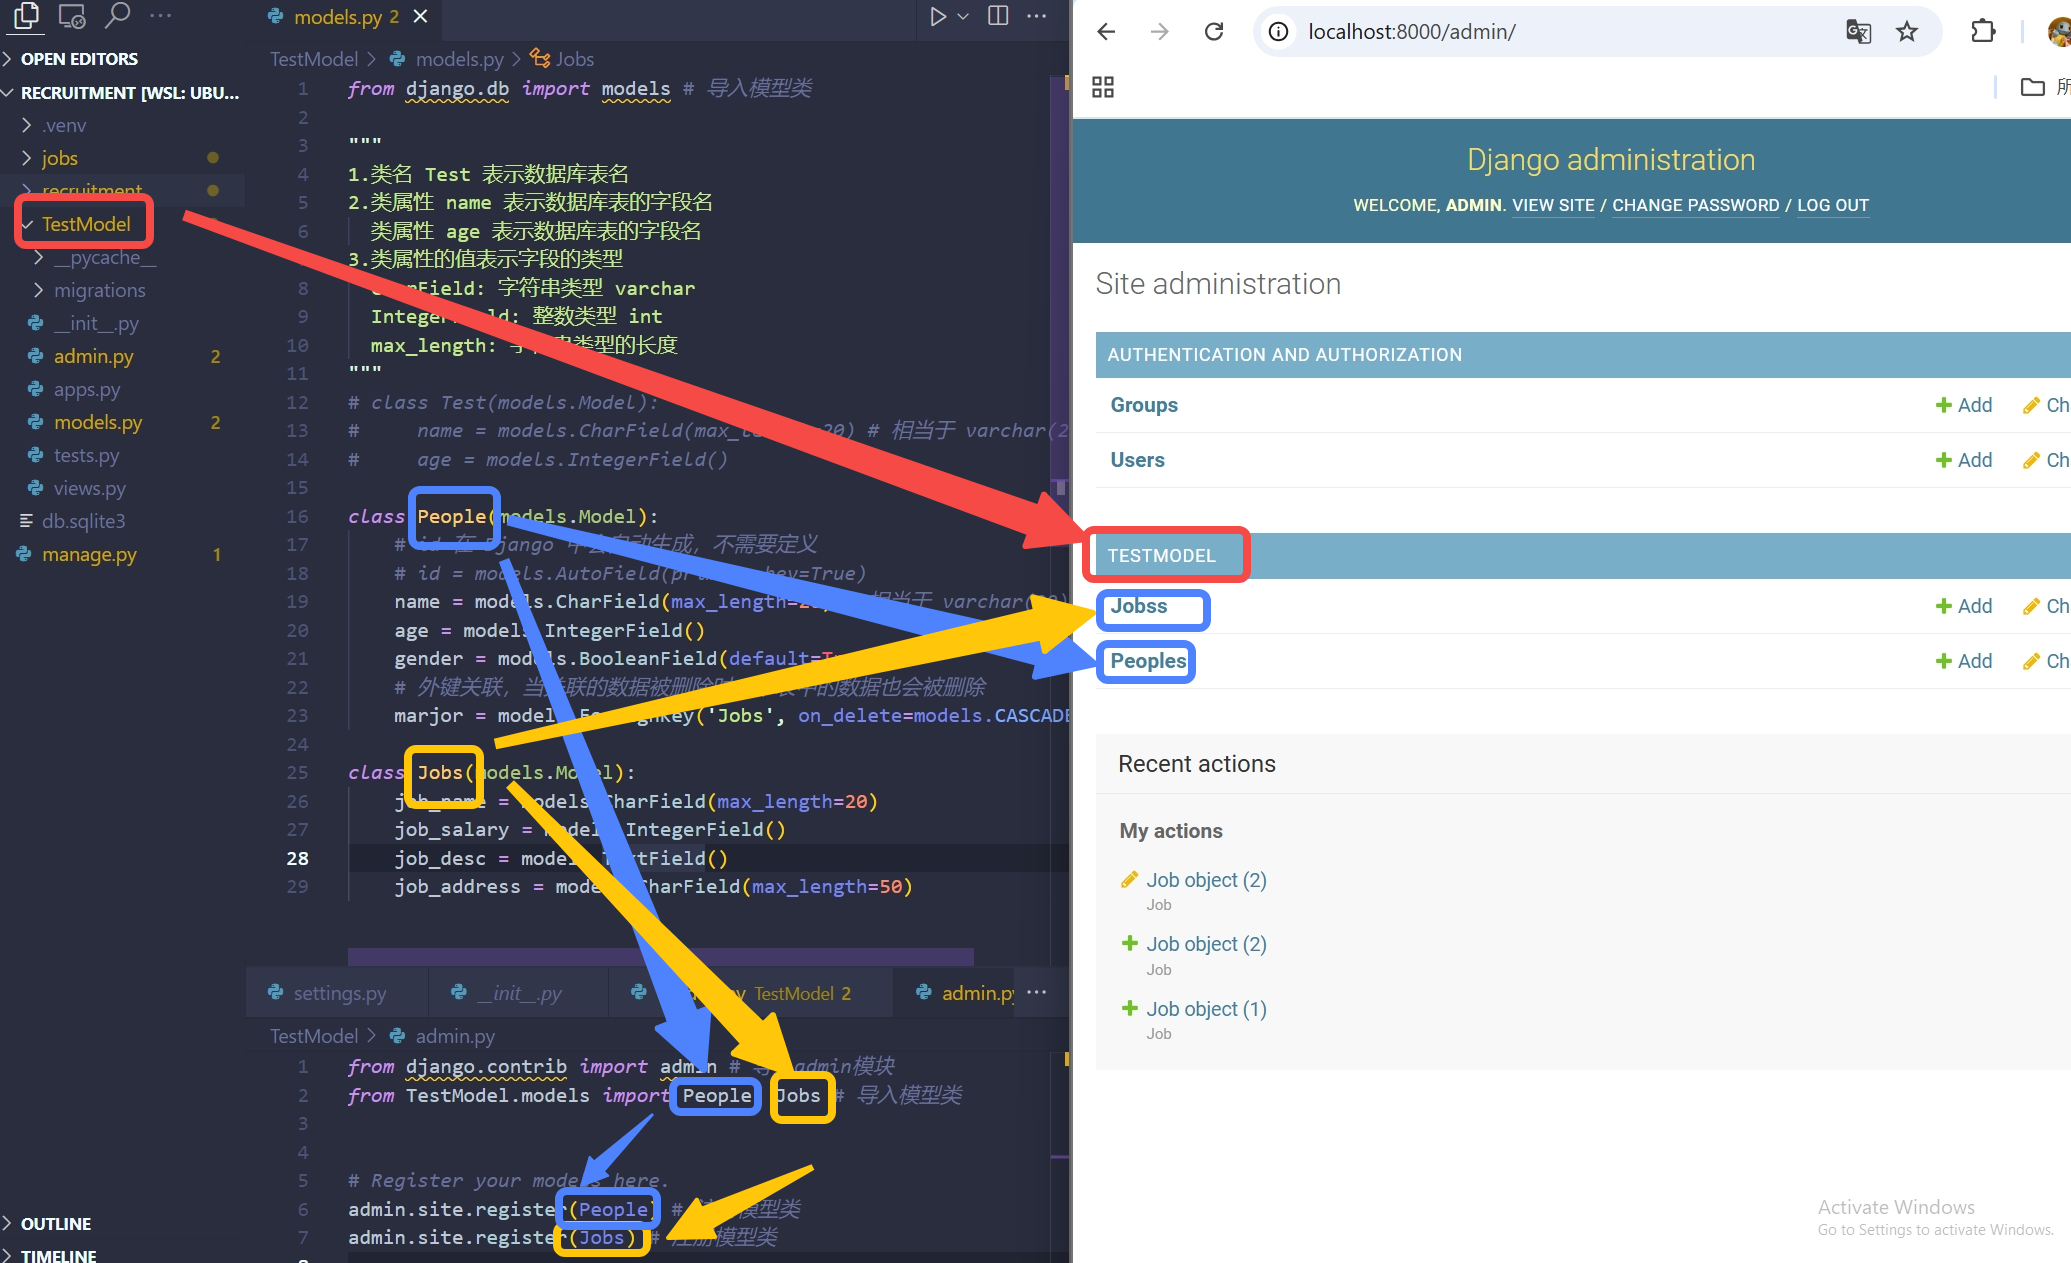
\includegraphics[width=0.6\textwidth]{part/互联/django/pic/模型/后台注册models.png}
    \caption{后台注册models}
    \label{fig:Django_后台注册models}
\end{figure}

如何对后台定义更多的信息，可以在模型类中设置\codeinline{Meta}类。
\begin{figure}[htpb]
    \centering
    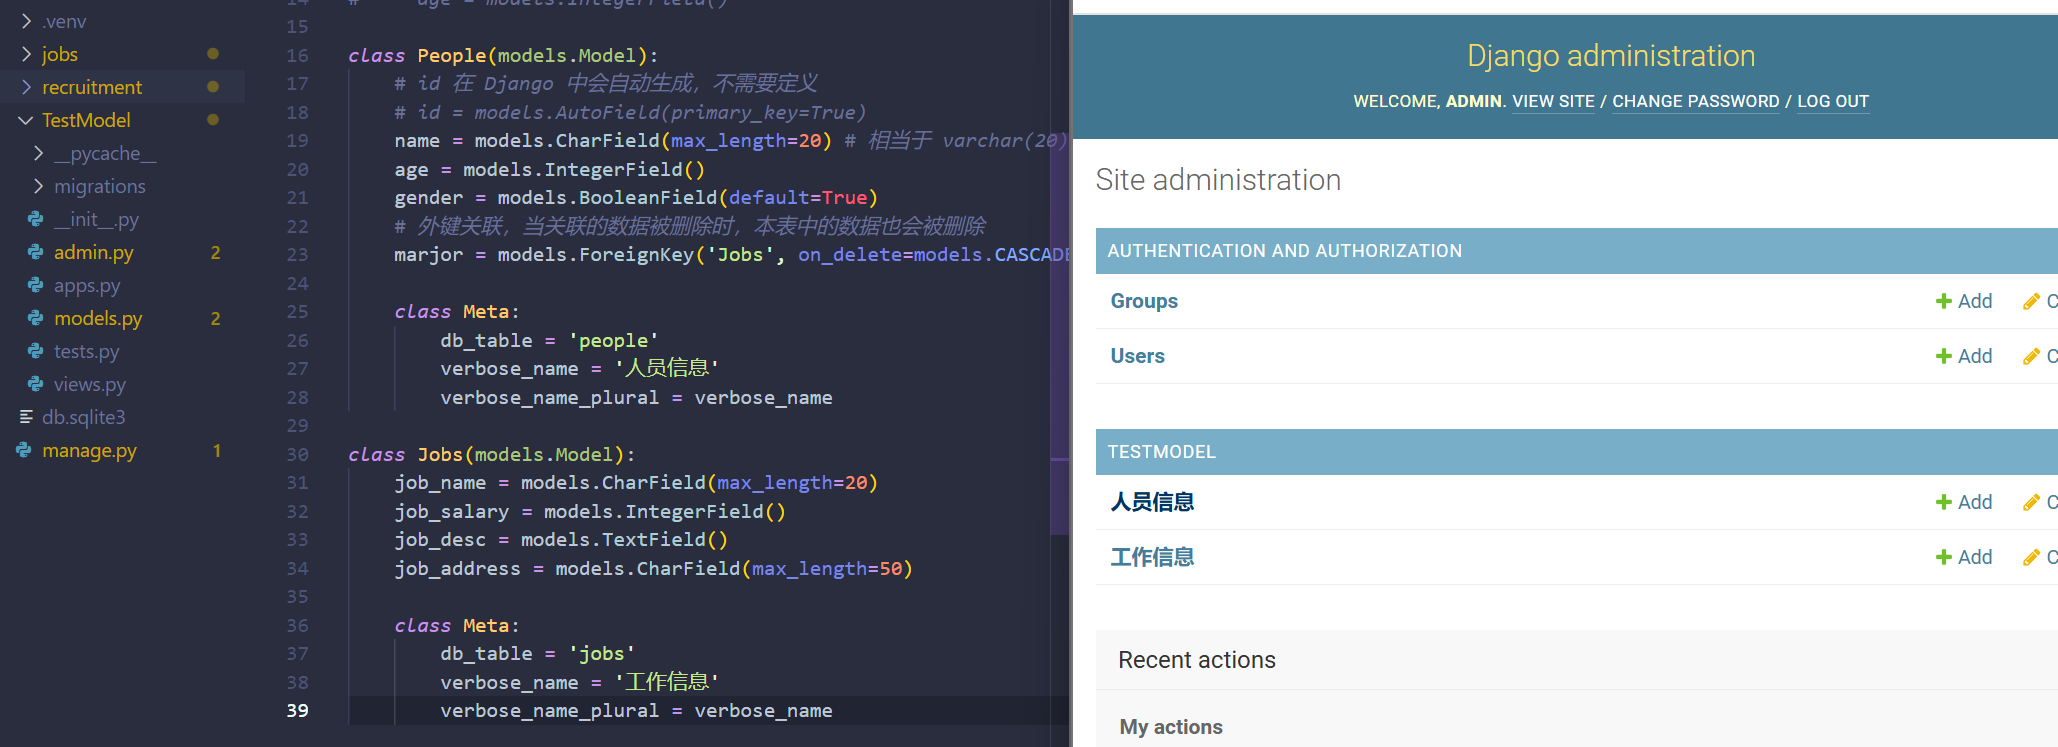
\includegraphics[width=0.6\textwidth]{part/互联/django/pic/模型/设置Meta信息.png}
    \caption{设置Meta信息}
    \label{fig:Django_设置Meta信息}
\end{figure}

如果想要在后台管理页面中显示更多的字段，可以在模型类中设置\codeinline{\_\_str\_\_()}方法。

如果想修改子应用在后台的名称，在子应用的\codeinline{apps.py}文件中设置\codeinline{verbose\_name}，如图\ref{fig:Django_修改子应用在后台的名称}所示。
\begin{lstlisting}[style=demostyle,numbers=none]
$> cat TestModel/apps.py
from django.apps import AppConfig


class TestmodelConfig(AppConfig):
    name = 'TestModel'
    verbose_name = '测试模型'

$> cat mysite/settings.py    
INSTALLED_APPS = [
    'django.contrib.admin',
    'django.contrib.auth',
    'django.contrib.contenttypes',
    'django.contrib.sessions',
    'django.contrib.messages',
    'django.contrib.staticfiles',
    # 'TestModel', # 添加创建的 app
    'TestModel.apps.TestmodelConfig', # 添加创建的 app
]
\end{lstlisting}
    
\begin{figure}[htpb]
    \centering
    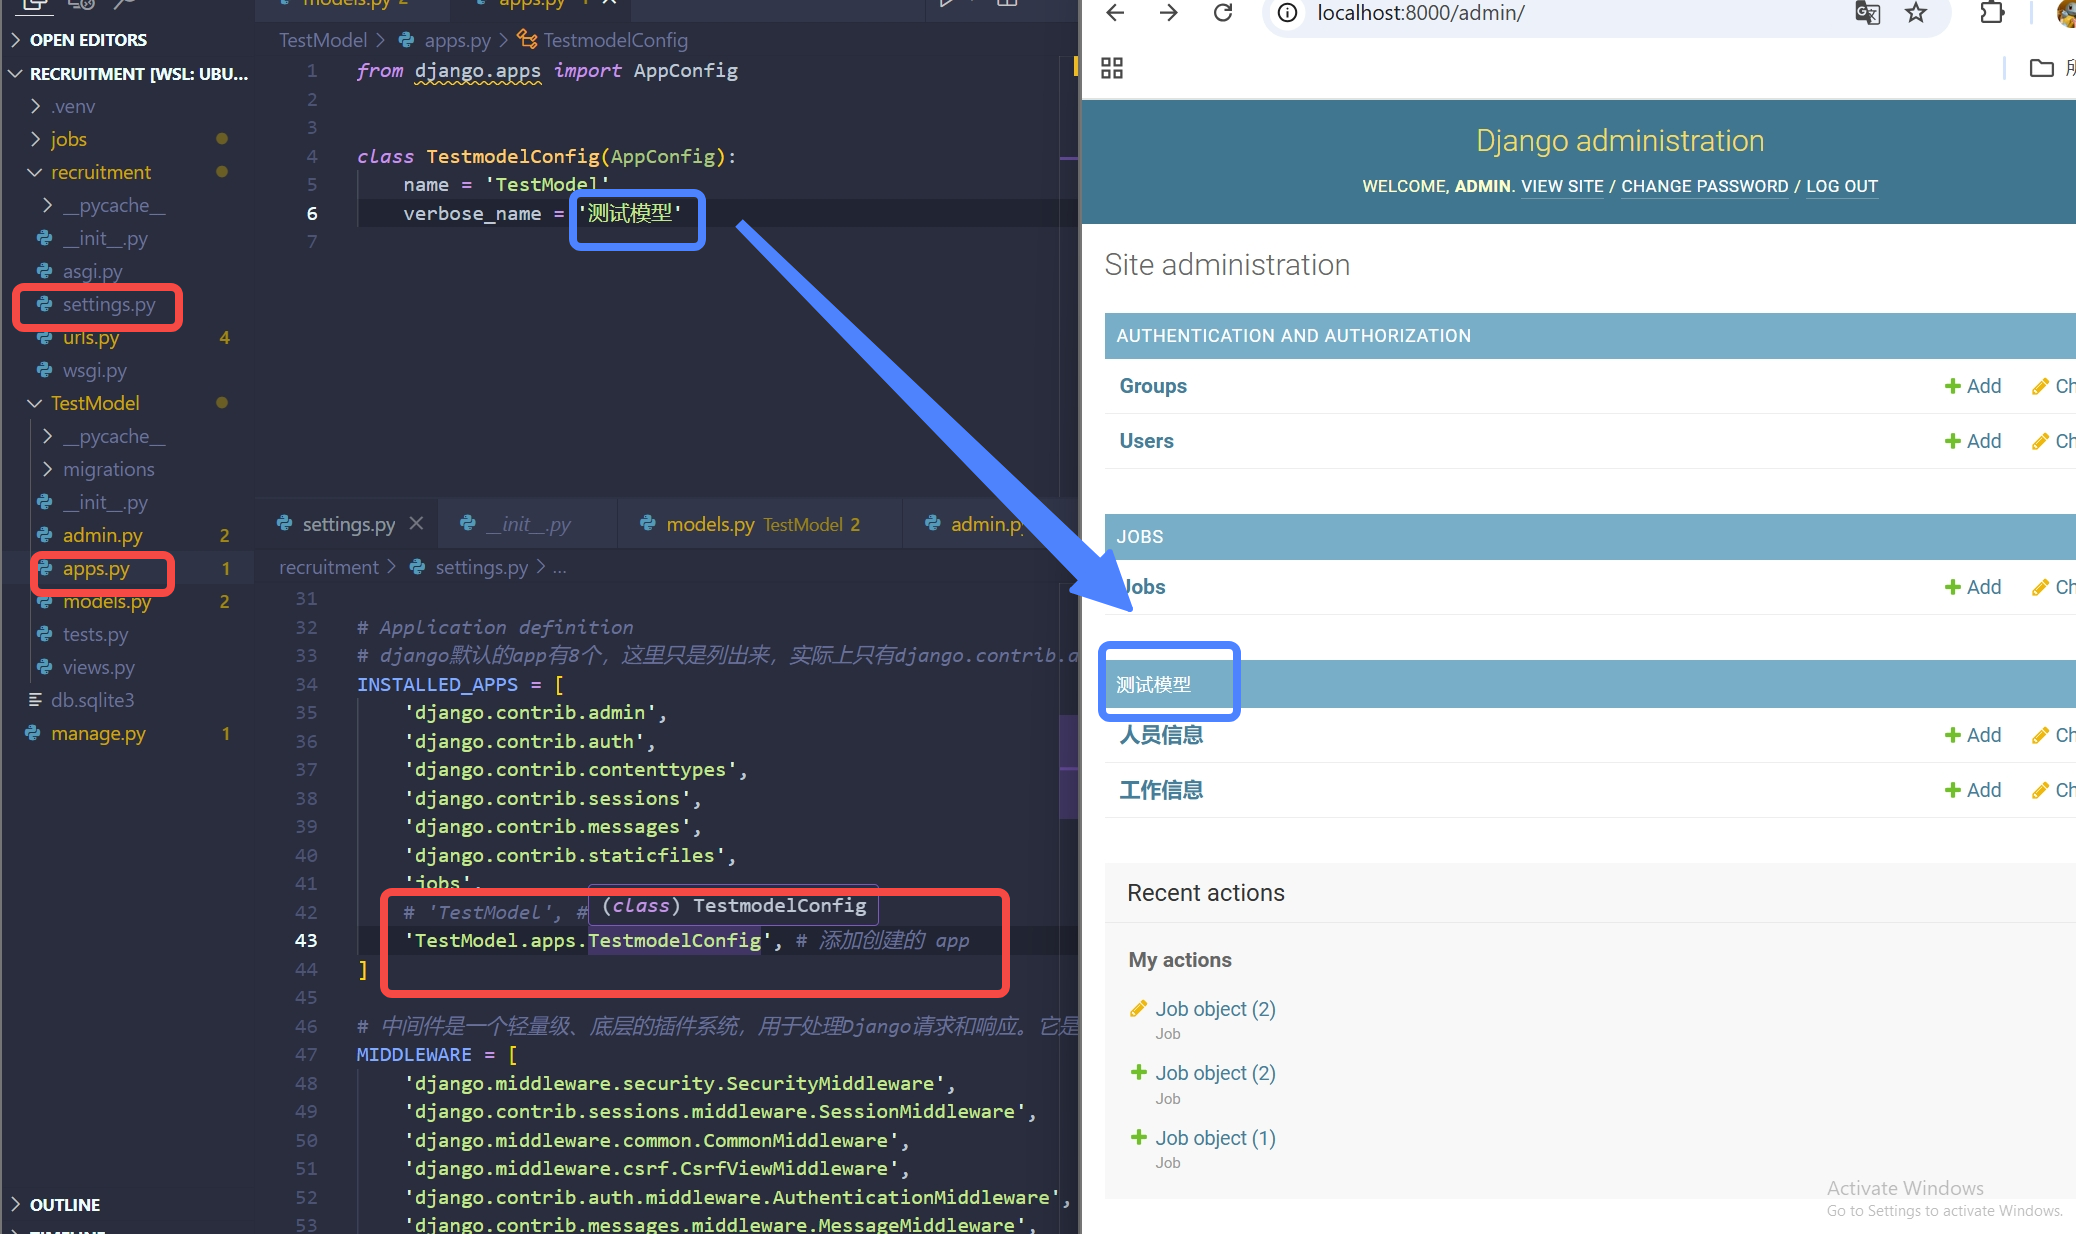
\includegraphics[width=0.6\textwidth]{part/互联/django/pic/模型/修改子应用在后台的名称.png}
    \caption{修改子应用在后台的名称}
    \label{fig:Django_修改子应用在后台的名称}
\end{figure}


\subsection{问题}
出现点击图\ref{fig:Django_设置Meta信息}中的子项出现404问题，解决方法如下：
\begin{figure}[htpb]
    \centering
    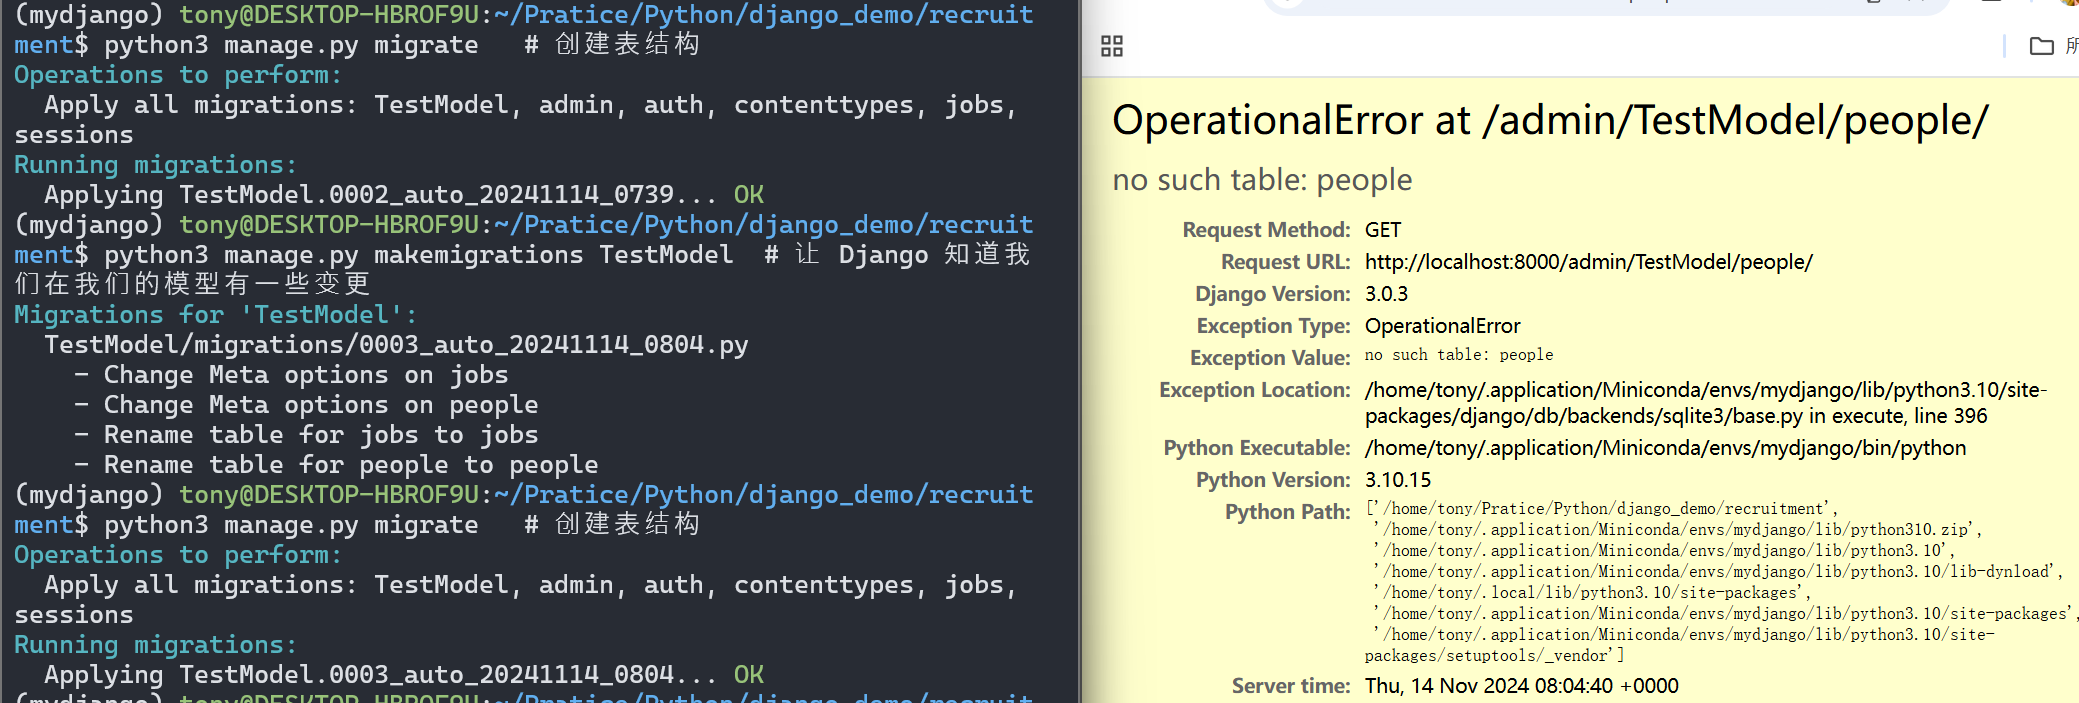
\includegraphics[width=0.4\textwidth]{part/互联/django/pic/模型/点击子项出现404问题.png}
    \caption{caption}
    \label{fig:label}
\end{figure}
\begin{lstlisting}[style=demostyle,numbers=none]
$ python3 manage.py makemigrations TestModel  # 让 Django 知道我们在我们的模型有一些变更
Migrations for 'TestModel':
  TestModel/migrations/0003_auto_20241114_0804.py
    - Change Meta options on jobs
    - Change Meta options on people
    - Rename table for jobs to jobs
    - Rename table for people to people

$ python3 manage.py migrate   # 创建表结构
Operations to perform:
  Apply all migrations: TestModel, admin, auth, contenttypes, jobs, sessions
Running migrations:
  Applying TestModel.0003_auto_20241114_0804... OK
\end{lstlisting}




\chapter{视图}
\section{视图}
Django 的视图是一个 Python 函数，它接受一个 Web 请求并返回一个 Web 响应。
Django 的视图可以以多种方式编写，最简单的方式是作为一个函数。

\section{视图函数}
\subsection{视图函数——HttpResponse}
视图函数是Django中的一个重要概念，它是一个Python函数，接收一个Web请求(\codeinline{request})并返回一个Web响应(\codeinline{HttpResponse})。
视图函数的定义如下：
\begin{lstlisting}[style=demostyle, numbers=none]
def my_view(request):
    # 业务逻辑
    return HttpResponse('Hello, World!')
\end{lstlisting}   

\subsection{渲染模板——render}
\begin{lstlisting}[style=demostyle, numbers=none]
render(request, '模板名称', {'参数1': '值1', '参数2': '值2'})    
\end{lstlisting}

\begin{enumerate}[label=\arabic*)]
    \item 在项目的根目录下创建一个\codeinline{templates}文件夹，用于存放模板文件。
    \item 在\codeinline{templates}文件夹下创建一个与子应用同名的文件夹\codeinline{TestModel}，
    用于存放子应用\codeinline{TestModel}的模板文件。

    \item 在\codeinline{TestModel}文件夹下创建一个\codeinline{test.html}文件，用于存放模板文件。
    \item 在主项目的\codeinline{settings.py}中配置模板路径。
\begin{lstlisting}[style=demostyle, numbers=none]    
$> cat mysite/settings.py
...
BASE_DIR = os.path.dirname(os.path.dirname(os.path.abspath(__file__)))
...
TEMPLATES = [
    {
        'BACKEND': 'django.template.backends.django.DjangoTemplates',
        # 'DIRS': [],
        'DIRS': [os.path.join(BASE_DIR, 'templates')], # 指定模板文件的目录
        'APP_DIRS': True,
        ...
    },
]
...
\end{lstlisting}    
    \item 在子应用目录下的\codeinline{urls.py}中，修改\codeinline{test\_view}函数，使用\codeinline{render}函数渲染模板。
\begin{lstlisting}[style=demostyle, numbers=none]
from django.urls import path
from .views import test_view, test_index

urlpatterns = [
    path('test/', test_view),
    path('index/', test_index),
]
\end{lstlisting}    
    \item 在子应用目录下\codeinline{views.py}中定义\codeinline{test\_index}函数，使用\codeinline{render}函数渲染模板。
\begin{lstlisting}[style=demostyle, numbers=none]
from django.shortcuts import render
from django.http import HttpResponse

# Create your views here.
def test_view(request):
    return HttpResponse('Hello, Django!') # 返回一个字符串

# 渲染模板 —— render

def test_index(request):
    return render(request, 'TestModel/index.html') # 渲染index.html模板
\end{lstlisting}    
    \item 在浏览器中输入\codeinline{http://localhost:8000/index/}，即可看到如图\ref{fig:Django渲染html的过程}所示页面。    
\end{enumerate}


\begin{figure}[htpb]
    \centering
    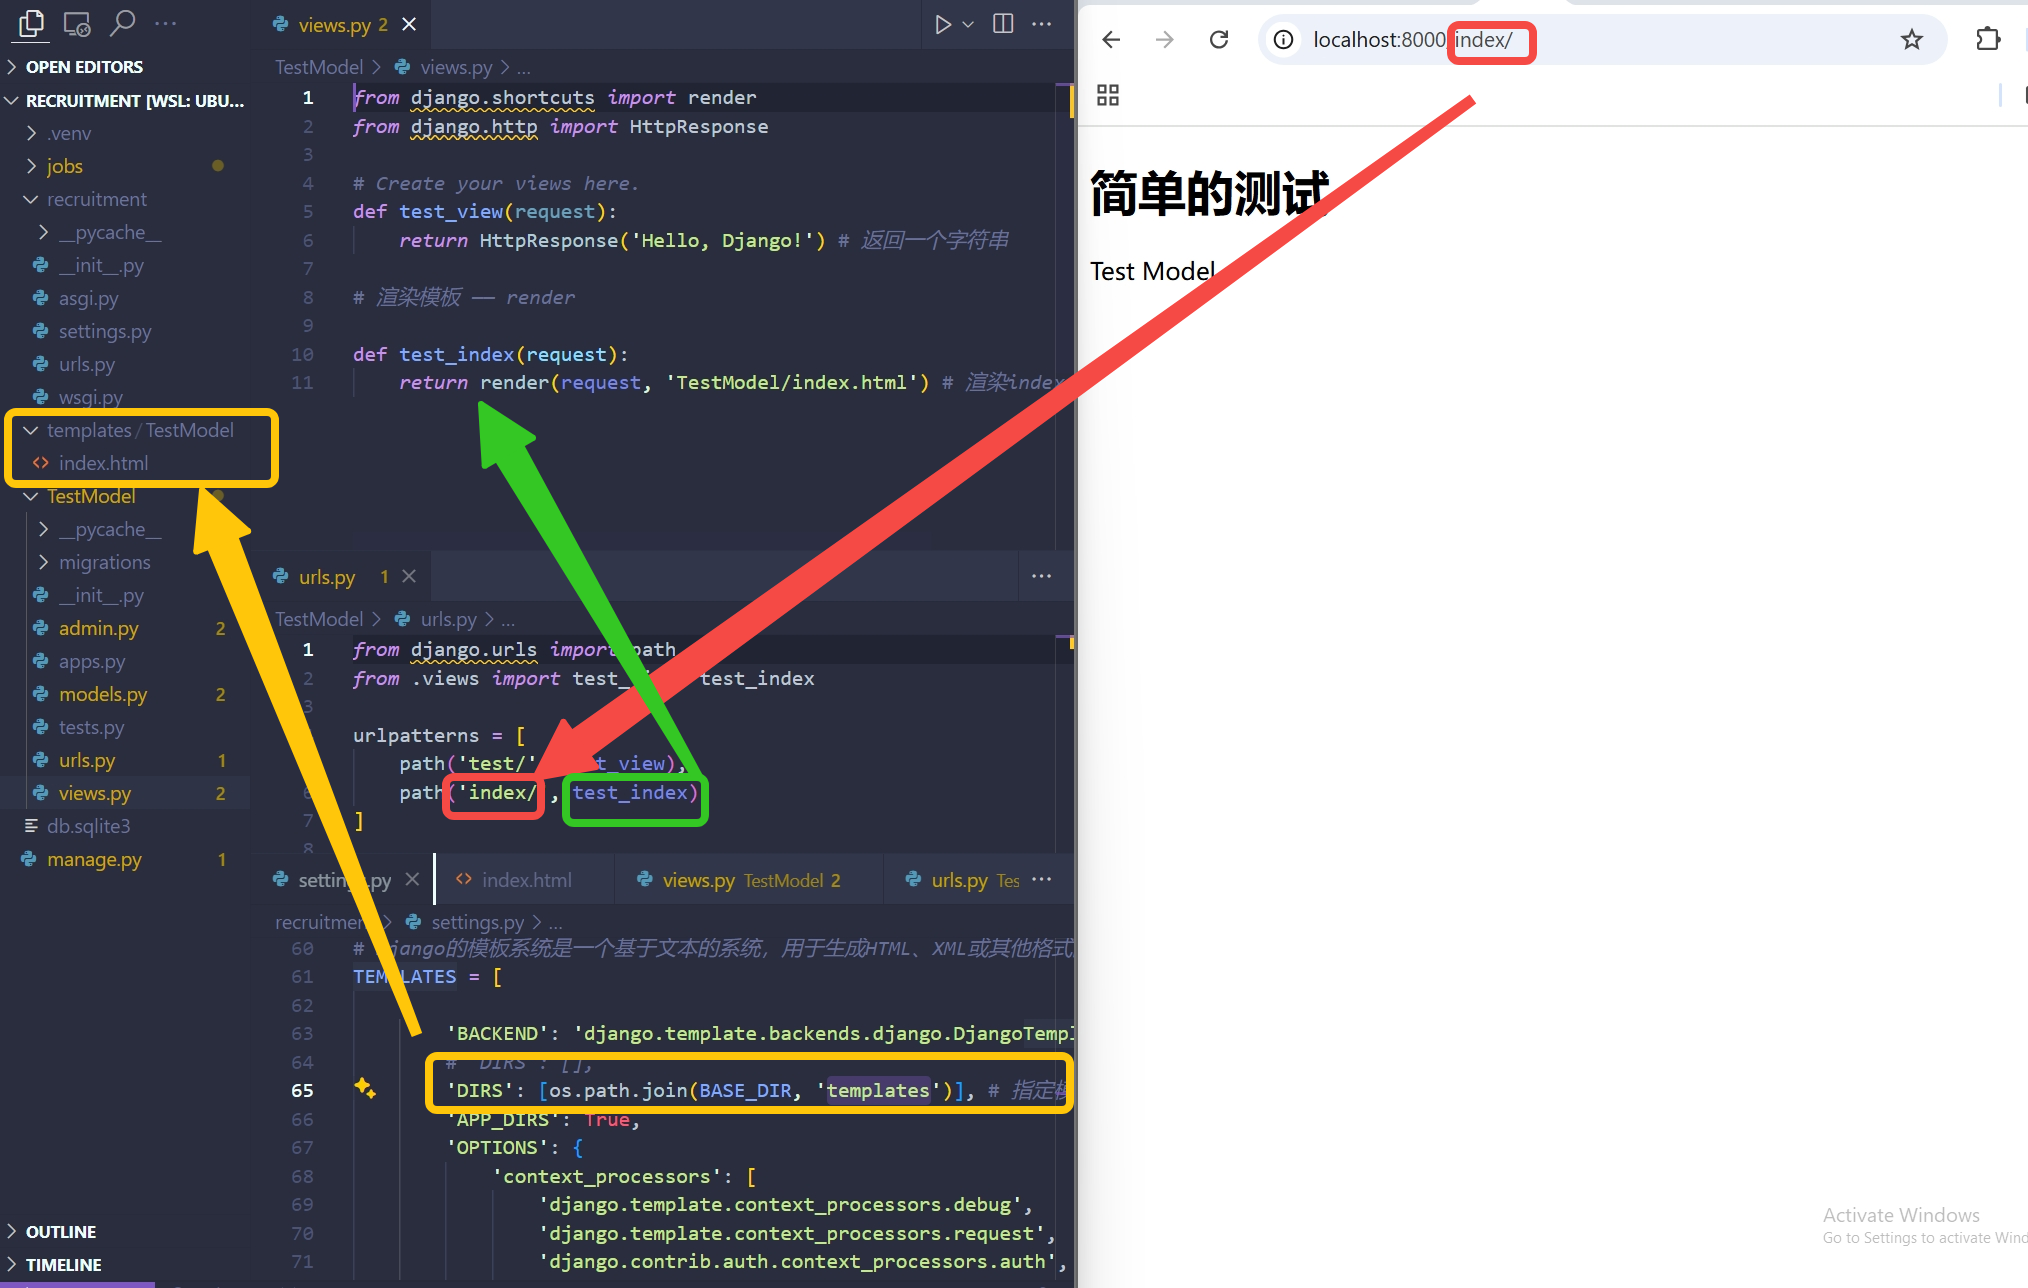
\includegraphics[width=0.6\textwidth]{part/互联/django/pic/视图/渲染html的过程.png}
    \caption{渲染html的过程}
    \label{fig:Django渲染html的过程}
\end{figure}

\section{URL配置(URLconf)}
URLconf 是 Django 中的 URL 配置，它是 URL 模式（URL 模式是 URL 和 Python 回调函数的映射）的集合。

一般在 \textcolor{YBXPurple}{主项目}目录下的\codeinline{urls.py}文件中配置 URLconf，用于将 URL 映射到 \textcolor{YBXPurple}{视图函数} 或 \codeinline{include}\textcolor{YBXPurple}{子应用}的 URLconf。

一般的格式为
\begin{enumerate}[label=\arabic*)]
    \item 主项目的\codeinline{urls.py}文件中，导入\codeinline{include}函数和子应用的\codeinline{urls.py}文件。
\begin{lstlisting}[style=demostyle,numbers=none]
from django.urls import path, include

urlpatterns = [
    # 直接引入视图函数
    path('路由名/', views.视图函数名),
    path('路由名/', views.视图函数名, name='视图函数名'),
    url(r'^路由名/', include('子应用.urls')),
    re_path(r'^路由名/', include('子应用.urls')),

    # 引入子应用的 URLconf
    path('子应用名/', include('子应用.urls')),
    url(r'^路由名/', include('子应用.urls')),
    re_path(r'^路由名/', include('子应用.urls')),
]
\end{lstlisting}
    
    \item 子应用的\codeinline{urls.py}文件中，导入视图函数。

\begin{lstlisting}[style=demostyle,numbers=none]
from django.urls import path, include
# 如果子应用有下面的一行，表示引入应用的 views.py 文件
from . import views    

urlpatterns = [
    path('路由名/', views.视图函数名),
    path('路由名/', views.视图函数名, name='视图函数名'),
]
\end{lstlisting}    
\end{enumerate}

\subsection{path() 将URL模式映射到视图}
\codeinline{path()}函数用于将 URL 模式映射到视图。

它采用四个参数，两个必选参数：route 和 view，两个可选参数：kwargs 和 name。
\begin{lstlisting}[style=demostyle,numbers=none]
from django.urls import path

path(route, view, kwargs=None, name=None)
\end{lstlisting}  
\begin{enumerate}[label=\arabic*)]
  \item \codeinline{route}: 字符串，定义 URL 的路径部分。
  
  可以包含变量，例如 \codeinline{<int:my\_variable>}，以从 URL 中捕获参数并将其传递给视图函数。

  \item \codeinline{view}: 视图函数，处理与给定路由匹配的请求。
  
  可以是一个函数或一个基于类的视图。
  
  \item \codeinline{kwargs}(可选): 一个字典，包含传递给视图函数的额外关键字参数。
  
  \item \codeinline{name}(可选): 为 URL 路由指定一个唯一的名称，以便在代码的其他地方引用它。这对于在模板中生成 URL 或在代码中进行重定向等操作非常有用。
\end{enumerate}

\subsection{[弃用] url()/re\_path 将URL模式映射到视图}
\codeinline{url()}函数用于将 URL 模式映射到视图。
\begin{lstlisting}[style=demostyle,numbers=none]
from django.urls import include, url

url(regex, view, kwargs=None, name=None, prefix=None)
\end{lstlisting}
\begin{enumerate}[label=\arabic*)]
  \item \codeinline{regex}: 字符串，包含正则表达式的 URL 模式。
  \item \codeinline{view}: 视图函数，处理与给定路由匹配的请求。
  \item \codeinline{kwargs}: 一个字典，包含传递给视图函数的额外关键字参数。
  \item \codeinline{name}: 为 URL 路由指定一个唯一的名称，以便在代码的其他地方引用它。
  \item \codeinline{prefix}: 字符串，用于给 URL 模式添加前缀。
\end{enumerate}

Django2. 0中可以使用 \codeinline{re\_path()}函数替代\codeinline{url()}函数。
\begin{lstlisting}[style=demostyle,numbers=none]
from django.urls import include, re_path

re_path(regex, view, kwargs=None, name=None)
\end{lstlisting}

\subsection{[不单独使用] include() 导入URL模式}
\codeinline{include()}函数用于包含其他 URL 模式。
\begin{lstlisting}[style=demostyle,numbers=none]
from django.urls import include

include(urlconf_module, namespace=None, app_name=None)
\end{lstlisting}
\begin{enumerate}[label=\arabic*)]
  \item \codeinline{urlconf\_module}: 字符串，包含 URL 模式的 Python 模块。
  \item \codeinline{namespace}: 字符串，用于给 URL 模式命名空间。
  \item \codeinline{app\_name}: 字符串，用于给 URL 模式命名空间。
\end{enumerate}

\begin{example}
    \exProblem
有下面的结构
\begin{lstlisting}[style=demostyle,numbers=none]
$ tree
.
|-- HelloWorld
|   |-- __init__.py
|   |-- __init__.pyc
|   |-- settings.py
|   |-- settings.pyc
|   |-- urls.py              # url 配置
|   |-- urls.pyc
|   |-- views.py              # 添加的视图文件
|   |-- views.pyc             # 编译后的视图文件
|   |-- wsgi.py
|   `-- wsgi.pyc
`-- manage.py
\end{lstlisting}  

其中\codeinline{views.py}文件内容如下：
\begin{lstlisting}[style=demostyle,numbers=none]
$> cat HelloWorld/views.py 文件代码：
from django.http import HttpResponse
 
def hello(request):
    return HttpResponse("Hello world ! ")
\end{lstlisting}
\exSolution

URL配置文件\codeinline{urls.py}有两种写法：
\begin{enumerate}[label=\arabic*)]
  \item 指向网站的根 URL
  \begin{lstlisting}[style=demostyle,numbers=none]
$> cat HelloWorld/urls.py 
from django.urls import path
 
from . import views
 
urlpatterns = [
    path("", views.hello, name="hello"),
]
\end{lstlisting}
\begin{figure}[htpb]
  \centering
  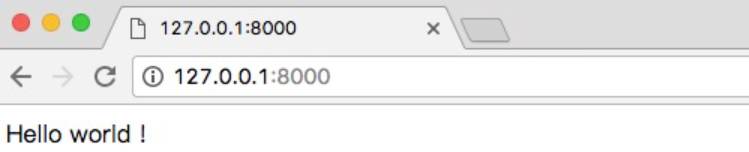
\includegraphics[width=0.4\textwidth]{part/互联/django/pic/概述/urlconf指向网站的根.png}
  \caption{urlconf指向网站的根}
  \label{fig:urlconf指向网站的根}
\end{figure}


  \item 适用于访问 \codeinline{/hello/} 路径
\begin{lstlisting}[style=demostyle,numbers=none]
$> cat HelloWorld/urls.py 
from django.urls import path
 
from . import views
 
urlpatterns = [
    path('hello/', views.hello),
]
\end{lstlisting}    
\begin{figure}[htpb]
  \centering
  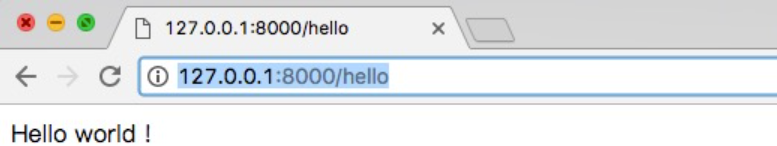
\includegraphics[width=0.4\textwidth]{part/互联/django/pic/概述/urlconf指向hello目录.png}
  \caption{urlconf指向hello目录}
  \label{fig:urlconf指向hello目录}
\end{figure}
  
\end{enumerate}
\end{example}

\section{路由视图过程}
\begin{enumerate}[label=\arabic*)]
    \item 在子应用\codeinline{TestModel}中的\codeinline{views.py}中定义一个\textcolor{YBXPurple}{视图函数}\codeinline{test\_view}，接收一个Web请求，返回一个Web响应。
    \item 在子应用\codeinline{TestModel}中的\textcolor{YBXPurple}{新建}一个\codeinline{urls.py}文件，定义一个\textcolor{YBXPurple}{路由}，将\codeinline{test\_view}与路由绑定。
\begin{lstlisting}[style=demostyle, numbers=none]
$> cat TestModel/urls.py
from django.urls import path
from .views import test_view

urlpatterns = [
    path('test/', test_view),
]
\end{lstlisting}    
    \item 在主应用\codeinline{mysite}中的\codeinline{urls.py}文件中，将子应用\codeinline{TestModel}的路由包含进来。
\begin{lstlisting}[style=demostyle, numbers=none]
from django.contrib import admin
from django.urls import path

from django.conf.urls import include, url

urlpatterns = [
    url(r"^", include('jobs.urls')), 
    path('admin/', admin.site.urls),  
    path('', include('TestModel.urls')),
]
\end{lstlisting}    
    \item 在浏览器中输入\codeinline{http://localhost:8000/test/}，即可看到如下页面：
\end{enumerate}

\begin{figure}[htpb]
    \centering
    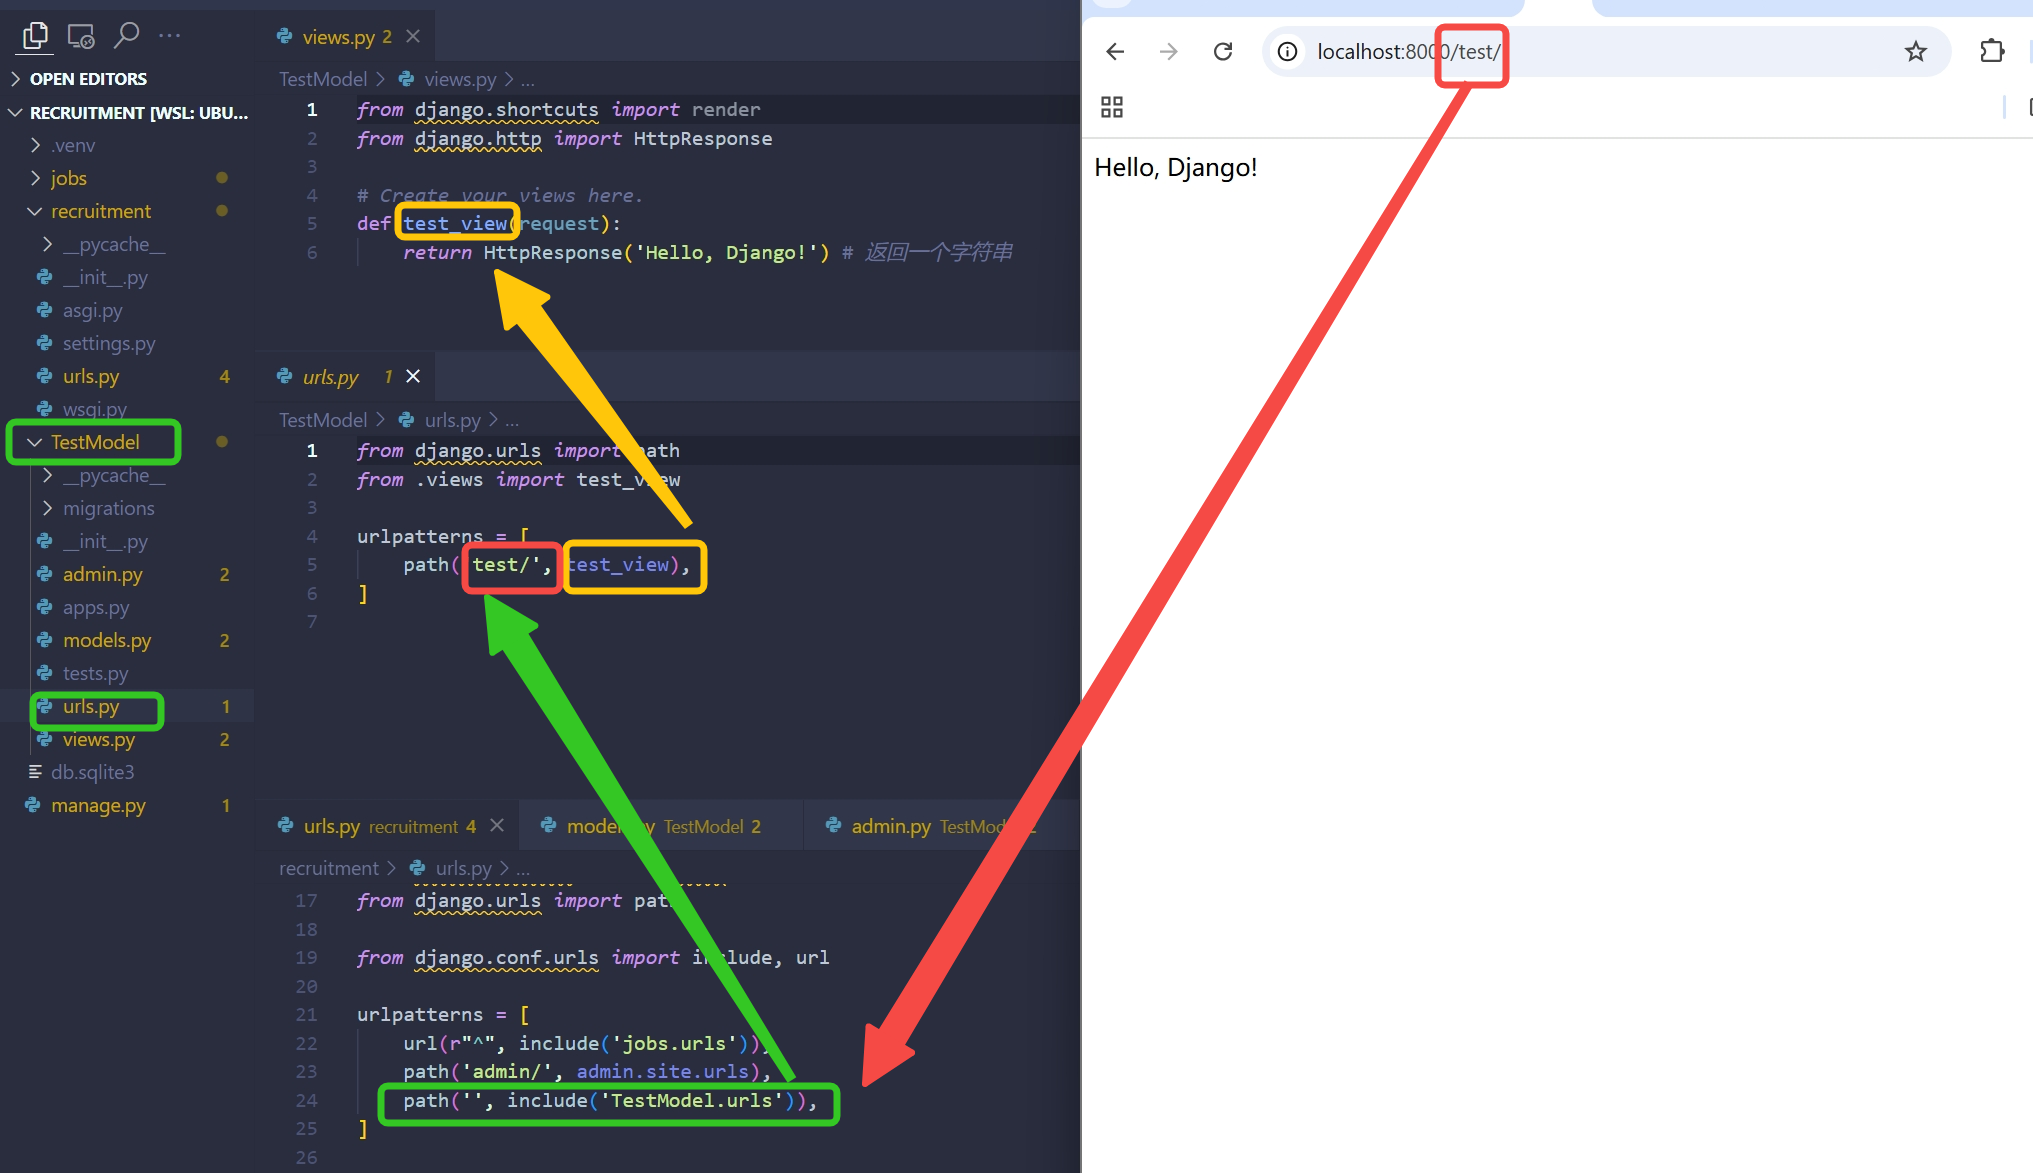
\includegraphics[width=0.6\textwidth]{part/互联/django/pic/视图/路由试图过程.png}
    \caption{路由视图过程}
    \label{fig:路由视图过程}
\end{figure}

其中路由的过程
\begin{enumerate}[label=\arabic*)]
    \item 用户在浏览器中输入\codeinline{http://localhost:8000/test/}。
    \item Django接收到请求，根据\codeinline{mysite/urls.py}中的路由配置，
    
    这里面是依次遍历\codeinline{jobs.urls}、\codeinline{admin}和\codeinline{TestModel.urls}。
    看这里面哪里个里面有\codeinline{test/}这个路由，找到了\codeinline{TestModel.urls}。

    \item 根据\codeinline{TestModel/urls.py}中的路由配置，找到了\codeinline{test\_view}。
    \item 调用\codeinline{test\_view}，返回一个\codeinline{HttpResponse}。
    \item 将\codeinline{HttpResponse}返回给浏览器。
\end{enumerate}








\chapter{模板template}
Django 模板是一个文本文件，它包含静态的 HTML，以及嵌入式的 Django 模板语言(DTL)代码。

\section{模板概述}
在Django中，创建一个\codeinline{base.html}文件，作为模板的基础文件，其他模板文件可以继承这个基础文件，从而减少重复代码。

\begin{enumerate}[label=\arabic*)]
  \item 一般在\textcolor{YBXPurple}{主项目根目录}创建一个\codeinline{templates}文件夹，用于存放模板文件。
\begin{lstlisting}[style=demostyle,numbers=none]
$> tree 
.
|-- manage.py
|-- TestModel  # 子应用
|   |-- admin.py
|   |-- apps.py
|   |-- views.py
|   |-- urls.py
|   |-- models.py
|   |-- tests.py
|   `-- migrate
|-- mysite   # 主项目目录
│   |-- __init__.py
│   |-- settings.py
│   |-- urls.py
│   `-- wsgi.py
`-- templates # 模板文件夹
\end{lstlisting}

  \item 在\textcolor{YBXPurple}{主项目}的\codeinline{settings.py}文件中配置模板文件路径。
    
\begin{lstlisting}[style=demostyle,numbers=none]
$> cat mysite/settings.py    
TEMPLATES = [
    {
        'BACKEND': 'django.template.backends.django.DjangoTemplates',
        # 'DIRS': [], # 之前的配置
        # 修改为
        'DIRS': [os.path.join(BASE_DIR, 'templates')],       
        'APP_DIRS': True,
        'OPTIONS': {
            'context_processors': [
                'django.template.context_processors.debug',
                'django.template.context_processors.request',
                'django.contrib.auth.context_processors.auth',
                'django.contrib.messages.context_processors.messages',
            ],
        },
    },
]
\end{lstlisting}

  \item 在\codeinline{templates}文件夹下创建一个\codeinline{base.html}文件，作为模板的基础文件，其他模板文件可以继承这个基础文件，从而减少重复代码。
\begin{lstlisting}[style=demostyle, numbers=none]
$> cat templates/base.html
<!DOCTYPE html>
<html lang="en">
<head>
    {% block delihead %}
    <meta charset="UTF-8">
    <meta name="viewport" content="width=device-width, initial-scale=1.0">
    <title>测试文件标题</title>
    <link rel="icon" href="static/images/logo.png">
    <link rel="stylesheet" href="static/style.css" type="text/css">
    {% endblock %}
</head>

<body>
    <h2>美使馆</h2>
    {% block content %}
    {% endblock %}
</body> 

<footer>
    <small>&copy 2020 美使馆<a href="http://www.baidu.com">JJW</a></small>
</footer>

</html>
\end{lstlisting}

  \item 在\codeinline{urls.py}文件中配置路径。
\begin{lstlisting}[style=demostyle,numbers=none]
$> cat urls.py
from django.urls import path
 
from . import views
 
urlpatterns = [
    path('hello/', views.hello),
]
\end{lstlisting}

\item 在\textcolor{YBXPurple}{子应用}的目录可以创建一个\codeinline{templates}文件夹，用于存放子应用的模板文件。
\begin{lstlisting}[style=demostyle,numbers=none]
$> tree TestModel
TestModel/
|-- __init__.py
|-- admin.py
|-- apps.py
|-- __pycache__
│   |-- __init__.cpython-39.pyc
│   |-- views.cpython-39.pyc
│   `-- urls.cpython-39.pyc
|-- templates
│   `-- hello.html
|--tests.py
|-- urls.py
`-- views.py
\end{lstlisting}  

其中 \codeinline{hello.html} 是子应用\codeinline{TestModel}的模板文件。
\begin{lstlisting}[style=demostyle,numbers=none]
$> cat templates/hello.html
{% extends 'base.html' %} <!-- 继承temples的base.html -->

{% block content %} <!-- 重写base.html的content -->
    <h3>Register</h3>
    <form action="/login/create_user" method="POST">
        {% csrf_token %}
        <input type="text" name="username" placeholder="Username" required>
        <input type="email" name="email" placeholder="Email" required>
        <input type="password" name="password" placeholder="Password" required>
        <input type="password" name="password2" placeholder="Confirm Password" required>
        <button type="submit">Register</button>
    </form>
{% endblock %}
\end{lstlisting}
  
  \item 在\textcolor{YBXPurple}{子应用}的\codeinline{views.py}文件中增加一个新的对象，
  用于向模板提交数据。
\begin{lstlisting}[style=demostyle,numbers=none]
$> cat TestModel/views.py
from django.shortcuts import render

"""
一个视图函数 hello
  接受一个 request 对象作为参数，并返回一个 HTTP 响应
"""
def hello(request):  
    context = {}     
    # context 是一个字典，用来存储传递给模板的上下文数据。在这个字典中，键是模板变量的名称，值是要传递给模板的实际数据。
    context['hello'] = 'Hello World!' 
    # 将 'Hello World!' 赋值给 context 字典中的 'hello' 键。这样，hello 将作为模板变量传递给模板，并且在模板中可以使用这个值。
    return render(request, 'hello.html', context)
\end{lstlisting}

  \item 启动服务器，访问\codeinline{http://localhost:8000/hello/}，可以看到页面显示\codeinline{Hello World!}。

\end{enumerate}

\subsection{模板的定义}
\begin{enumerate}[label=\arabic*)]
    \item 模板变量：\codeinline{\{\{ 变量名 \}\}}
    \item 从URL获取模板变量
\begin{lstlisting}[style=demostyle, numbers=none]
{% url '路由名' 参数 %}    
\end{lstlisting}    

\begin{example}
    \exProblem
    在\codeinline{urls.py}中定义一个
\begin{lstlisting}[style=demostyle, numbers=none]
re_path('(?P<year>[0-9]{4}).html', views.myyear, name='urlyear'),        

# 1.(?P<year>[0-9]{4})：
这是正则表达式中的一个命名捕获组，(?P<year>[0-9]{4})的含义是匹配4位数字（0-9之间），并将匹配到的内容命名为year。
# 2.views.myyear：当URL匹配成功后，Django会调用 views.myyear 这个视图函数，并将匹配到的 year 参数传递给它。
例如，如果URL是 2023.html，那么 views.myyear 会接收到 year=2023。
# 3.name='urlyear'：
这是给这个URL模式起的一个名字，方便在Django的其他地方通过名称来引用该URL。
通过这个名字，你可以使用 reverse() 函数或 {% url %} 模板标签来生成对应的URL，例如 {% url 'urlyear' year=2023 %} 会生成 2023.html。
\end{lstlisting}    


    
而在模板文件夹的\codeinline{test.html}中，
\begin{lstlisting}[style=demostyle, numbers=none]
<a href="{% url 'urlyear' 2019 %}">2019年度</a>
\end{lstlisting}        
    \exSolution

    当找到\codeinline{test.html}模板文件时，会到\codeinline{urls.py}中找到\codeinline{urlyear}这个路由，
    并将\codeinline{2019}作为参数传递给\codeinline{myyear}函数。
    从而在浏览器中显示\codeinline{2019年度}的超链接。

\begin{lstlisting}[style=demostyle, numbers=none]
<a href="/2019.html">2019年度</a>
\end{lstlisting}            
    
\end{example}

    \item 读取静态资源内容
\begin{lstlisting}[style=demostyle, numbers=none]
{% static "css/style.css" %} 
\end{lstlisting}
    \item for遍历：\codeinline{\{\% for 变量名 in 列表名 \%\}}
\begin{lstlisting}[style=demostyle, numbers=none]
{% for item in list %}
    {{ item }}
{% endfor %}    
\end{lstlisting}
    \item if判断：\codeinline{\{\% if 条件 \%\}}
\begin{lstlisting}[style=demostyle, numbers=none]
{% if 条件 %}
    {{ 变量 }}
{% endif %}
\end{lstlisting}       
\end{enumerate}


\section{静态文件}

\subsection{静态文件的作用}

静态文件是指不需要经过服务器处理，直接可以被浏览器访问的文件，例如：图片、CSS、JavaScript等。

\begin{enumerate}[label=\arabic*)]
    \item 图片：\codeinline{.jpg}、\codeinline{.png}、\codeinline{.gif}等。
    \item CSS：\codeinline{.css}文件，用于设置网页的样式。
    \item JavaScript：\codeinline{.js}文件，用于设置网页的交互效果。
\end{enumerate}

\subsection{静态文件的配置}
\begin{enumerate}[label=\arabic*)]
  \item 在 \textcolor{YBXPurple}{主项目}的\codeinline{settings.py}文件中配置静态文件路径。
\begin{lstlisting}[style=demostyle,numbers=none]
STATIC_URL = '/static/'
if not DEBUG:
    STATIC_ROOT = os.path.join(BASE_DIR, 'static')

# 重写 STATICFILES_DIRS    
STATICFILES_DIRS = (os.path.join(BASE_DIR, 'static'),) # 必须是一个元组(,)要有,
\end{lstlisting} 

  \item 想要引用static资源文件的\textcolor{YBXPurple}{子项目}，
  需要在\textcolor{YBXPurple}{子项目}的\codeinline{urls.py}文件中的\codeinline{urlpatterns}列表中添加一条配置，
  用于访问静态文件。

\begin{lstlisting}[style=demostyle,numbers=none]
from django.urls import path
from . import views  # Import the views module

from django.conf import settings
from django.conf.urls.static import static

urlpatterns = [
    path("", views.open_register, name="open register"),  
    
] + static(settings.STATIC_URL, document_root=settings.STATICFILES_DIRS[0]) 
# 在 settings.py 中配置了 STATICFILES_DIRS，所以这里可以直接使用 settings.STATICFILES_DIRS[0] 来获取静态文件目录
\end{lstlisting} 
\end{enumerate}

在\textcolor{YBXPurple}{子项目}的视图\codeinline{views.py}中，可以通过\codeinline{render}函数将静态文件传递给模板。
\begin{lstlisting}[style=demostyle,numbers=none]
from django.shortcuts import render
from django.template import loader
from django.http import HttpResponse

# Create your views here.
def open_register(request):
    template = loader.get_template('login/register.html')
    return HttpResponse(template.render({}, request))
\end{lstlisting}








\part{数据处理与分析}
%% Pandas
\chapter{[Python库] Pandas}
\label{cha:pandas_intro}
\section{简介}
\label{sec:pandas_intro}
\href{https://pandas.pydata.org/}{Pandas}是一个开源的数据分析库，
它为Python编程语言提供了高性能、易于使用的数据结构和数据分析工具。

它基于一种叫作 DataFrame 的数据结构，
这种数据结构模仿了 R 语言中的 DataFrame。
简单来说，一个 pandas DataFrame 是一张表格，类似于 Excel 表格。
pandas 中包含大量用于修改表格和操作表格的方法，尤其是可以像 SQL 一样对表格进行查询和连接。
NumPy 要求数组中的所有元素类型必须完全相同，而 pandas 不是这样，
每一列数据的类型可以互不相同（比如整型、日期、浮点数和字符串）。

pandas 的另一个强大之处在于，它可以从许多文件格式和数据库中提取数据，
如SQL、Excel 文件和逗号分隔值（CSV）文件。

\section{安装}
\label{sec:install_pandas}
\begin{lstlisting}[style=demostyle,numbers=none]
# 安装
conda install pandas
# 或
pip install pandas
\end{lstlisting}




\chapter{Pandas的数据结构}
\label{cha:pandas_data_structure}
\section{Series}
\label{sec:pandas_series}


\section{DataFrame}
\label{sec:pandas_dataframe}

\section{Index}
\label{sec:pandas_index}




\chapter{Pandas数据的引用和读取}
\label{cha:pandas_reference_read}

\section{数据的引用}
\label{sec:pandas_reference}


\section{文件的读取与写入}
\label{sec:pandas_read_write}

\subsection{CSV}
\label{subsec:pandas_read_csv}

\subsection{Excel}
\label{subsec:pandas_read_excel}


\subsection{JSON}
\label{subsec:pandas_read_json}

\subsection{HDF5}
\label{subsec:pandas_read_hdf5}


\chapter{Pandas数据的聚合和排序}
\label{cha:pandas_aggregate_sort}






\part{人工智能}
% \input{part/深度学习框架/Tensorflow/Tensorflow概述.tex}
\chapter{PyTorch}
\section{概述}
PyTorch是一个Python的开源机器学习库，是Python优先的深度学习框架。
PyTorch是科学计算框架Torch在Python上的衍生，PyTorch的产生受到了 Torch和Chainer这两个框架的启发。
Torch使用Lua作为开发语言，PyTorch则使用了 Python作为开发语言。 
与Chainer类似，PyTorch具有自动求导的动态图功能，也就是所谓的define by run,即当Python解释器运行到相应的行时才创建计算图。

PyTorch就像带GPU的NumPy,采用了动态计算图（Dynamic Computational Graph）结构，
是基于tape的autograd系统的深度神经网络。通过PyTorch的一种称为\textcolor{blue}{\textbf{反向模式自动微分}}
（Reverse-Mode Auto Differentiation） 的技术，我们可以非常方便地构建网络。

\codeinline{torch}是PyTorch的核心库，提供了很多用于创建和操作张量的函数。

PyTorch由4个主要包组成，具体如下
\begin{enumerate}[label=\arabic*)]
    \item \codeinline{torch}
    类似于NumPy的通用数组库，可将张量类型转换为\codeinline{torch.cuda.TensorFloat},并在GPU上进行计算。

    \item \codeinline{torch.autograd}
    用于构建计算图形并自动获取梯度的包。
    
    \item \codeinline{torch.nn}
    神经网络构建的包，包括各种神经网络层，损失函数等。

    \item \codeinline{torch.optim}
    优化器，包括各种优化算法，如SGD、Adam等。

    \item \codeinline{torch.utils}
    数据处理工具，包括数据集加载、数据增强等。
\end{enumerate}

\subsection{与TensorFlow的比较}
\begin{enumerate}[label=\arabic*)]
    \item 运行机制
    两个框架都是在张量上进行运算，并将任意一个模型看成是有向无环图
    (Direct Acyclic Graph, DAG),但TensorFlow遵循“数据即代码，代码即数据”的理念，
    当在TensorFlow中运行代码时，DAG是以静态方式定义的，若需要实现动态DAG,则需要借助TensorFlow Fold库；
    
    而PyTorch属于更Python化的框架，动态DAG是内置的，可以随时定义、随时更改、
    随时执行节点，并且没有特殊的会话接口或占位符，相当灵活

    \item 训练模式
    在分布式训练中，TensorFlow和PyTorch的一个主要差异特点是数据并行化，
    使用TensorFlow时，使用者必须手动编写代码，并微调在特定设备上运行的每个操作，
    以实现分布式训练；
    
    而PyTorch则是利用异步执行的本地支持来实现的，其自身在分布式中的训练是比较欠缺的。

    \item 可视化
    在可视化方面，TensorFlow内置的TensorBoard非常强大，能够显示模型图，
    绘制标量变量，实现图像、嵌入可视化，甚至是播放音频等功能：
    
    PyTorch的可视化情况，则显得有点差强人意，开发者可以使用Visdom,
    但是Visdom提供的功能很简单且有限，可视化效果远远比不上TensorBoard。

    \item 生产部署
    对于生产部署而言，TensorFlow具有绝对的优势，它可以直接使用TensorFlow Serving 在TensorFlow中部署模型；
    
    而PyTorch没有提供任何用于在网络上直接部署模型的框架， 需要使用Flask或者另一种替代方法来基于模型编写一个RESTAPI。
\end{enumerate}


\section{PyTorch的历史}
这里的 Py 我们不陌生，它就是 Python，那 Torch 是什么？从字面翻译过来是一个“火炬”。

什么是火炬呢？其实这跟 TensorFlow 中的 Tensor 是一个意思，我们可以把它看成是能在 GPU 中计算的矩阵。

那 PyTorch 框架具体是怎么用的呢？说白了就是一个计算的工具。借助它，我们就能用计算机完成复杂的计算流程。

但是我们都知道，机器跟人类的“语言”并不相通，想要让机器替我们完成对数据的复杂计算，就得先把数据翻译成机器能够理解的内容。无论是图像数据、文本数据还是数值数据，都要转换成矩阵才能进行后续的变化和运算。

搞定了读入数据这一步，我们就要靠 PyTorch 搞定后面各种复杂的计算功能。这些所有的计算功能，
包括了从前向传播到反向传播，甚至还会涉及其它非常复杂的计算，
而这些计算统统要交给 PyTorch 框架实现。

PyTorch 会把我们需要计算的矩阵传入到 GPU（或 CPU）当中，在 GPU（或 CPU）中实现各种我们所需的计算功能。因为 GPU 做矩阵运算比较快，
所以在神经网络中的计算一般都首选使用 GPU，但对于学习来说，我们用 CPU 就可以了。

\section{PyTorch的主要应用}
PyTorch主要应用于以下几个方面：
\begin{enumerate}[label=\arabic*)]
    \item 计算机视觉:使用PyTorch,程序员可以处理图像和视频，开发高度准确和精确的计算机视觉模型，如图像分类模型、对象检测模型和生成模型等。
    \item 自然语言处理:PyTorch可用于开发语言翻译、语言建模和聊天机器人等。利用PyTorch,程序员可使用长短期记忆网络、门控循环单元等处理自然语言、时间序列等方面的任务。
    \item 强化学习:PyTorch可用于开发强化学习模型，如深度Q网络、策略梯度
\end{enumerate}

\section{Pytorch环境搭建}
\subsection{前提条件}
Windows平台还需要安装Microsoft Visual C++ (VC\_redist.x64.exe),
可从\href{https://docs.microsoft.com/zh-CN/cpp/windows/latest-supported-vc-redist}{微软网站}下载安装最新支持的 Visual C++。

\subsection{CPU版本}
对于CPU版本直接通过pip或者anaconda命令安装即可，如：
\begin{lstlisting}[style=demostyle,numbers=none]
pip install torch torchvision torchaudio
\end{lstlisting}

\subsection{GPU版本}
目前PyTorch不仅支持NVIDIA的GPU，还支持AMD的ROCm的GPU。

对于N卡，什么型号是pytorch支持的呢？首先，需要计算能力（compute capability）$\geq$3.0的GPU。
可以到\href{https://developer.nvidia.cn/zh-cn/cuda-gpus}{NVIDIA官网}查看支持的GPU型号。


\href{https://pytorch.org/get-started/locally/}{本地下载}

\subsubsection{conda安装}
\begin{lstlisting}[style=demostyle,numbers=none]
conda create --name mypytorch python=3.10    
# 安装 CUDA 12.1 版本    
conda install pytorch torchvision torchaudio pytorch-cuda=12.1 -c pytorch -c nvidia
## pytorch 是 PyTorch 的核心库，提供了深度学习的基本功能
## torchvision 是基于 PIL 的 Python 图像库，主要用于图像处理和计算机视觉任务
## torchaudio 是 PyTorch 的音频库，提供了一些音频处理的工具
## pytorch-cuda=12.1 是指定安装的 CUDA 版本
## -c pytorch -c nvidia 是指定安装的渠道

# 验证pytorch是否安装成功
python -c "import torch; print(torch.__version__)"

$ python
Python 3.10.14 (main, May  6 2024, 19:42:50) [GCC 11.2.0] on linux
Type "help", "copyright", "credits" or "license" for more information.
>>> import torch
nt(torch.__version__)
>>> print(torch.__version__)
2.4.0
>>> print(torch.cuda.is_available())
True
>>> print(torch.version.cuda)
12.1
>>>
\end{lstlisting}

\subsubsection{whl安装}
如果网速不好的话，\href{https://download.pytorch.org/whl/torch}{Pytroch离线下载whl}搜索对应的whl进行下载。

若是手动下载的whl，需要注意pytorch与torchvision之间版本对应关系，这个可以到\href{https://github.com/pytorch/vision}{torchvision Github}查看，这点非常重要，CV中一些报错就是因为torchvision与pytorch版本不匹配导致的。
\begin{lstlisting}[style=demostyle,numbers=none]
pip install *.whl
\end{lstlisting}

\subsection{问题}
为什么我安装的明明是 GPU 版本，但是代码却返回了“False”，显示 GPU 不可用呢？
\begin{enumerate}[label=\arabic*)]
    \item 检查计算机上是否有支持 CUDA 的 GPU
    首先查看电脑的显卡型号以及是否有独立显卡，如果没有以“NVIDIAN”名称开头的独立显卡，则不能支持 CUDA，因此 GPU 不可用

    \item 检查显卡驱动版本。
    在终端中输入“\codeinline{nvidia-smi}”命令，会显示出显卡驱动的版本和 CUDA 的版本。

    如果显卡驱动的版本过低，与 CUDA 版本不匹配，那么 GPU 也不可用，需要根据显卡的型号更新显卡驱动。

    \item 检查 PyTorch 版本和 CUDA 版本是否匹配
    
\end{enumerate}

\subsection{后续辅助}
完成PyTorch库的安装后，还需要安装辅助库，如绘图库Matplotlib>数据分析库 pandas以及开发编辑工具Jupyter Notebook等，
可在Anaconda Prompt命令行或者终端执行以下安装命令。
\begin{lstlisting}[style=demostyle,numbers=none]
pip install pandas matplotlib notebook
\end{lstlisting}


\section{PyTorch 模块结构}
\subsection{Torch 相关}
torch 是 PyTorch 框架的核心库，提供了深度学习的基本功能。

\subsubsection{PyTorch 安装目录}
通过\codeinline{conda info --envs}命令查看当前环境下的所有虚拟环境的位置。
\begin{lstlisting}[style=demostyle,numbers=none]
$ conda info --envs
# conda environments:
#
base                     /home/tony/.application/Miniconda
mypytorch                /home/tony/.application/Miniconda/envs/mypytorch

# 因此PyTorch的安装位置在
/home/tony/.application/Miniconda/envs/mypytorch/lib/python3.10/site-packages/
\end{lstlisting}

\begin{figure}[htpb]
    \centering
    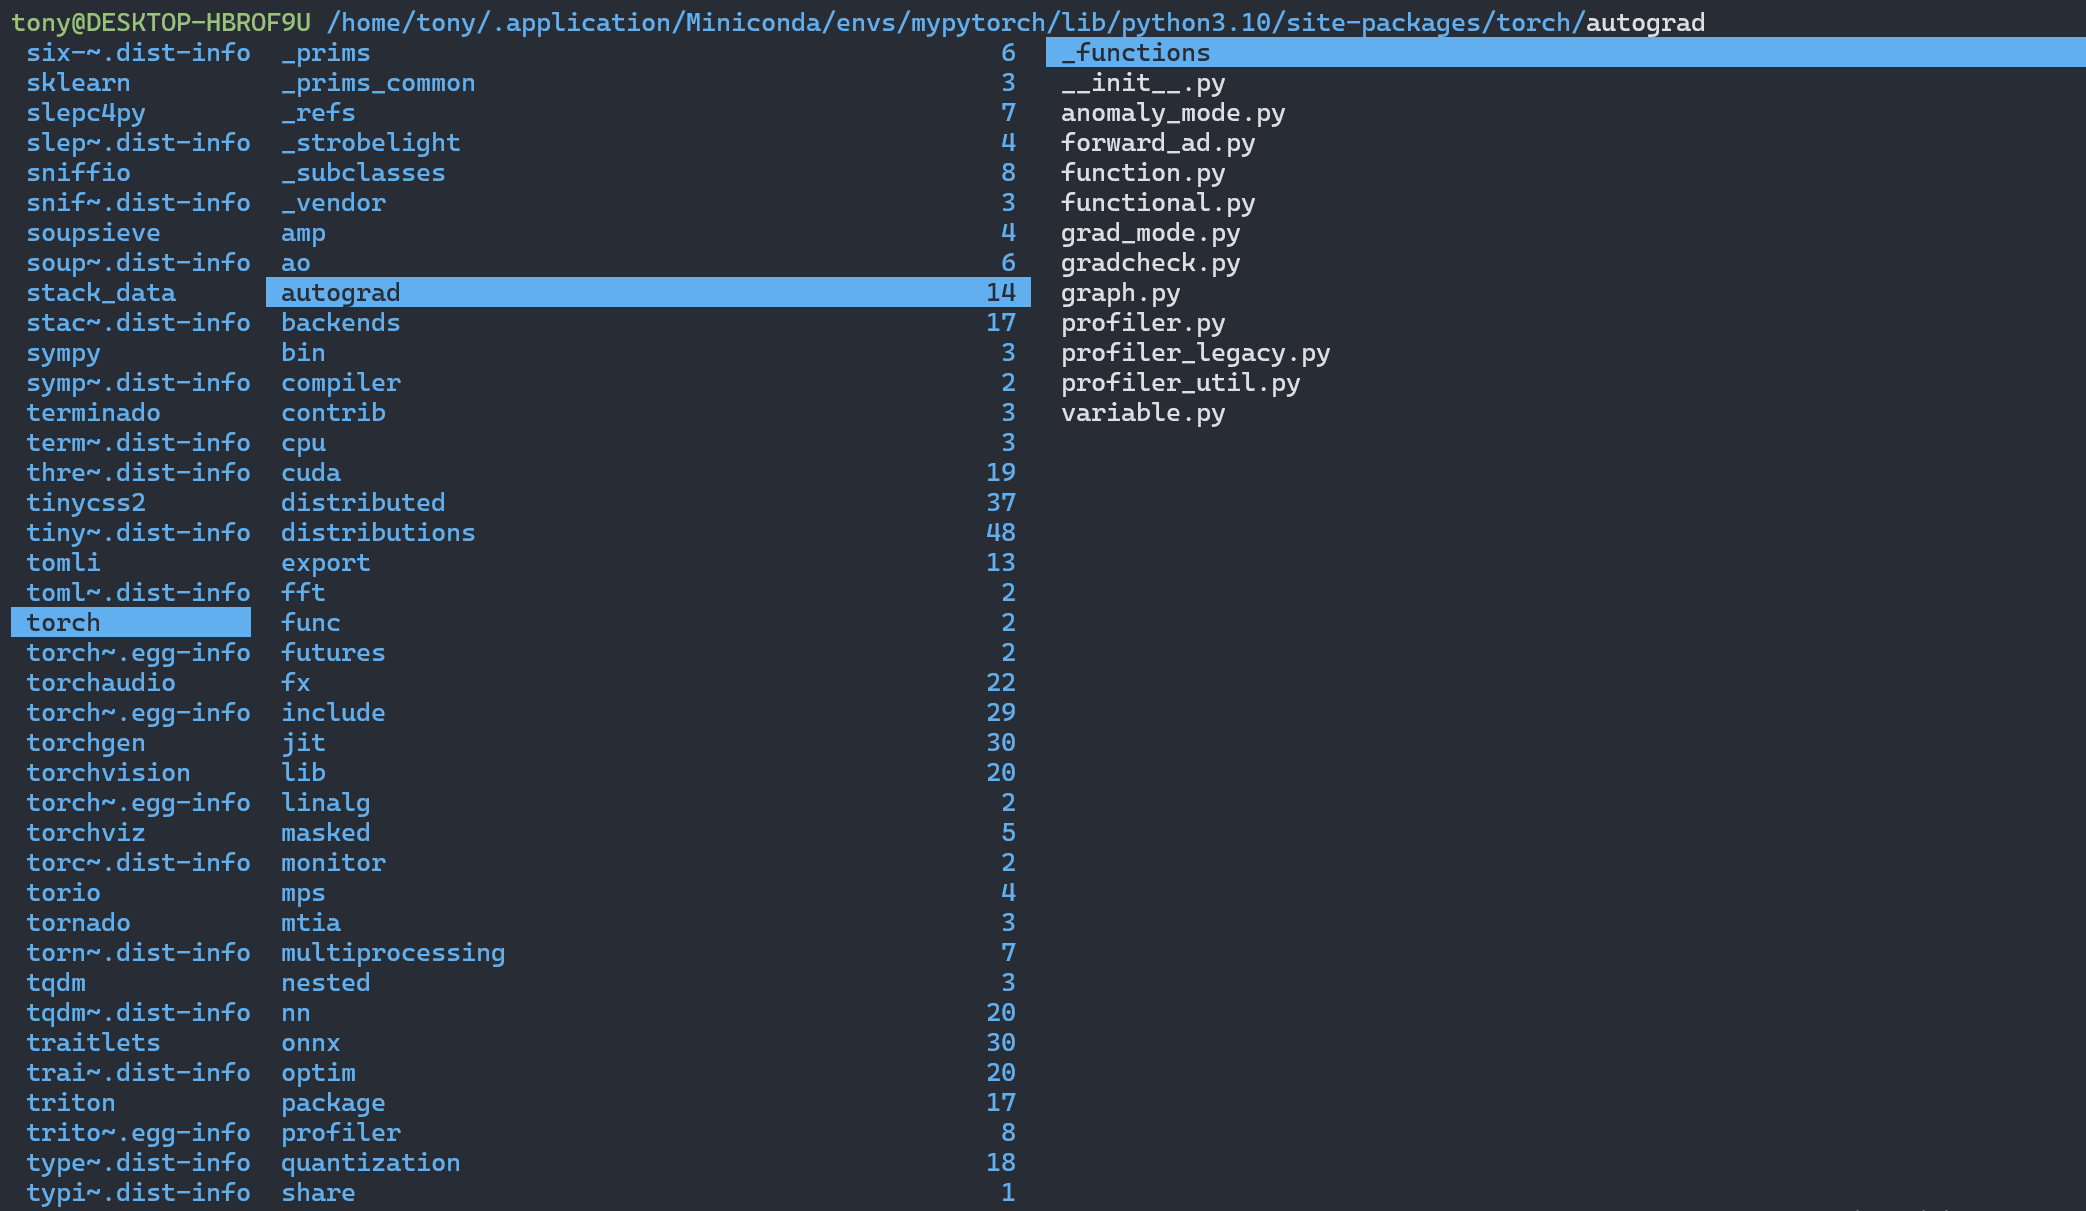
\includegraphics[width=0.6\textwidth]{part/人工智能/深度学习框架/pic/Pytorch/PyTorch概述/PyTorch安装目录.png}
    \caption{PyTorch安装目录}
    \label{fig:PyTorch安装目录}
\end{figure}

\subsubsection{PyTorch的主要模块}
\begin{enumerate}[label=\arabic*)]
    \item \_C

    从文件夹名称就知道它和C语言有关，其实它是辅助C语言代码调用的一个模块，该文件夹里存放了一系列pyi文件，
    pyi文件是python用来校验数据类型的，如果调用数据类型不规范，会报错。
    
    PyTorch的底层计算代码采用的是C++语言编写，并封装成库，供pytorch的python语言进行调用。
    这一点非常重要，后续我们会发现一些pytorch函数无法跳转到具体实现，这是因为具体的实现通过C++语言，我们无法在Pycharm中跳转查看。

    \item include
    
    上面讲到pytorch许多底层运算用的是C++代码，那么C++代码在哪里呢？
    它们在这里,在torch/csrc文件夹下可以看到各个\codeinline{.h/.hpp}文件，而在python库中，只包含头文件，这些头文件就在include文件夹下。

    但如果直接下载的是PyTorch的whl文件，是没有这个文件夹的，因为这个文件夹是源码编译的时候才会有的。

    \item lib
    
    torch文件夹中最重要的一个模块，torch文件夹占3.2GB的空间，98\%的内容都在lib中，占了3.16GB空间。
    pytorch的内容几乎都在lib里面，让我们看看里面是什么。
    
    lib文件夹下包含大量的.lib .so文件（分别是静态链接库和动态链接库），例如大名鼎鼎的\codeinline{libcudnn\_*.so}， \codeinline{libc*\_cuda.so}。
    这些底层库都会被各类顶层python api调用。

    \item autograd：自动求导，自动计算张量的梯度，用于反向传播
    
    该模块是pytorch的核心模块与概念，它实现了梯度的自动求导，
    极大地简化了深度学习研究者开发的工作量，开发人员只需编写前向传播代码，反向传播部分由\codeinline{autograd}自动实现，
    再也不用手动去推导数学公式，
    然后编写代码了（很多朋友可能不知道，在早期的深度学习框架中是没有这个功能的，例如caffe，它需要手动编写反向传播的公式代码）
    \begin{figure}[htpb]
        \centering
        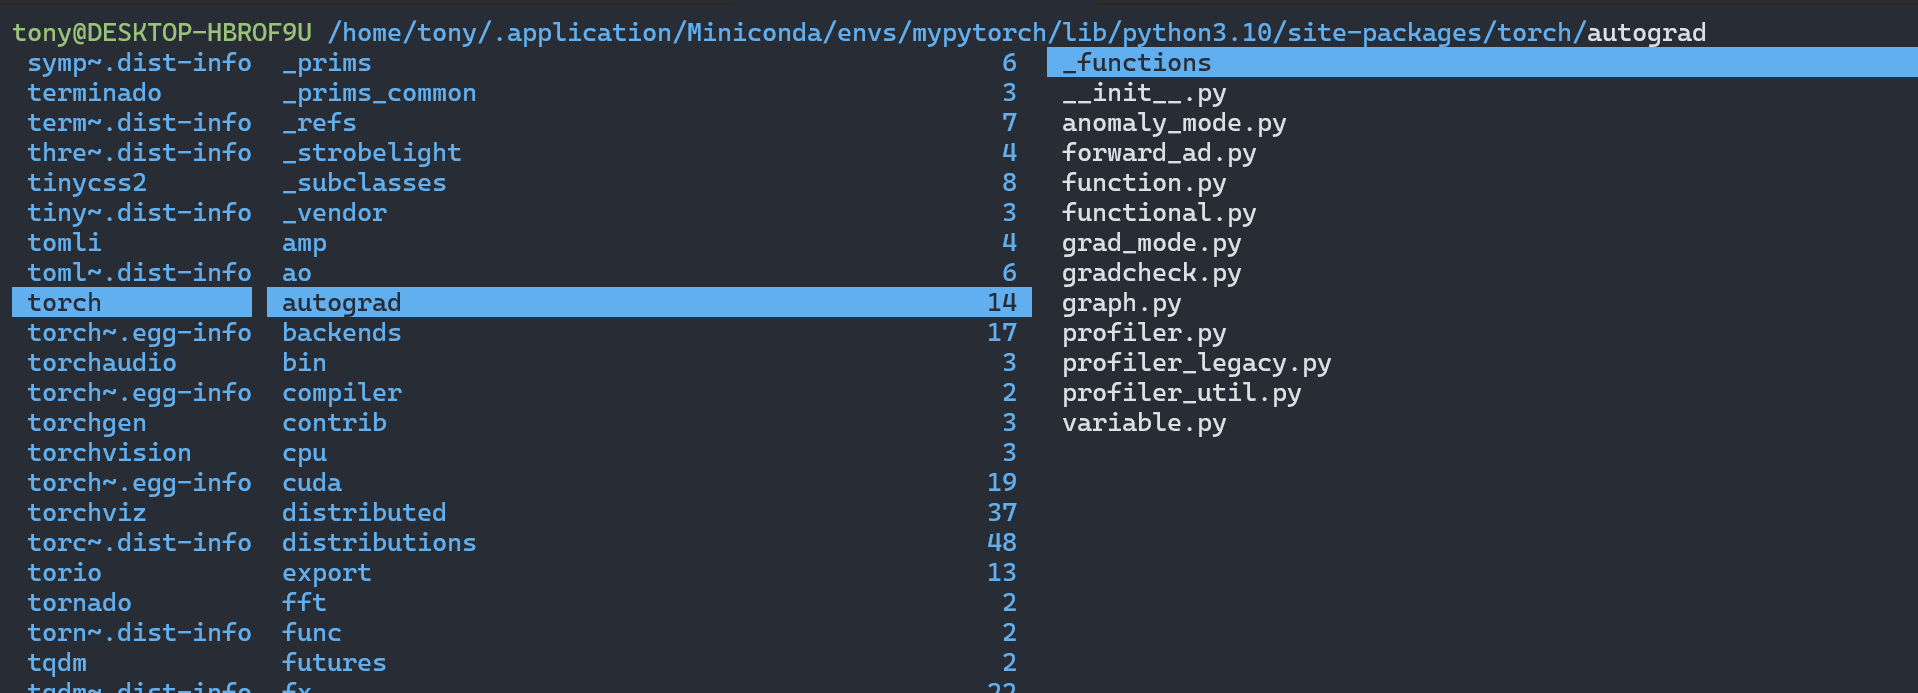
\includegraphics[width=0.6\textwidth]{part/人工智能/深度学习框架/pic/Pytorch/PyTorch概述/autograd中的算法.png}
        \caption{autograd中的算法}
        \label{fig:autograd中的算法}
    \end{figure}
    
    
    \item nn：神经网络模块
    
    相信这个模块是99\%pytorch开发者使用频率最高的模块，
    搭建网络的网络层就在\codeinline{nn.modules}里边。
    我们可以到\codeinline{torch/nn/modules}里面看常用的网络层，
    包括常见的层（如全连接层、卷积层、循环层等）以及损失函数。
    
    \begin{figure}[htpb]
        \centering
        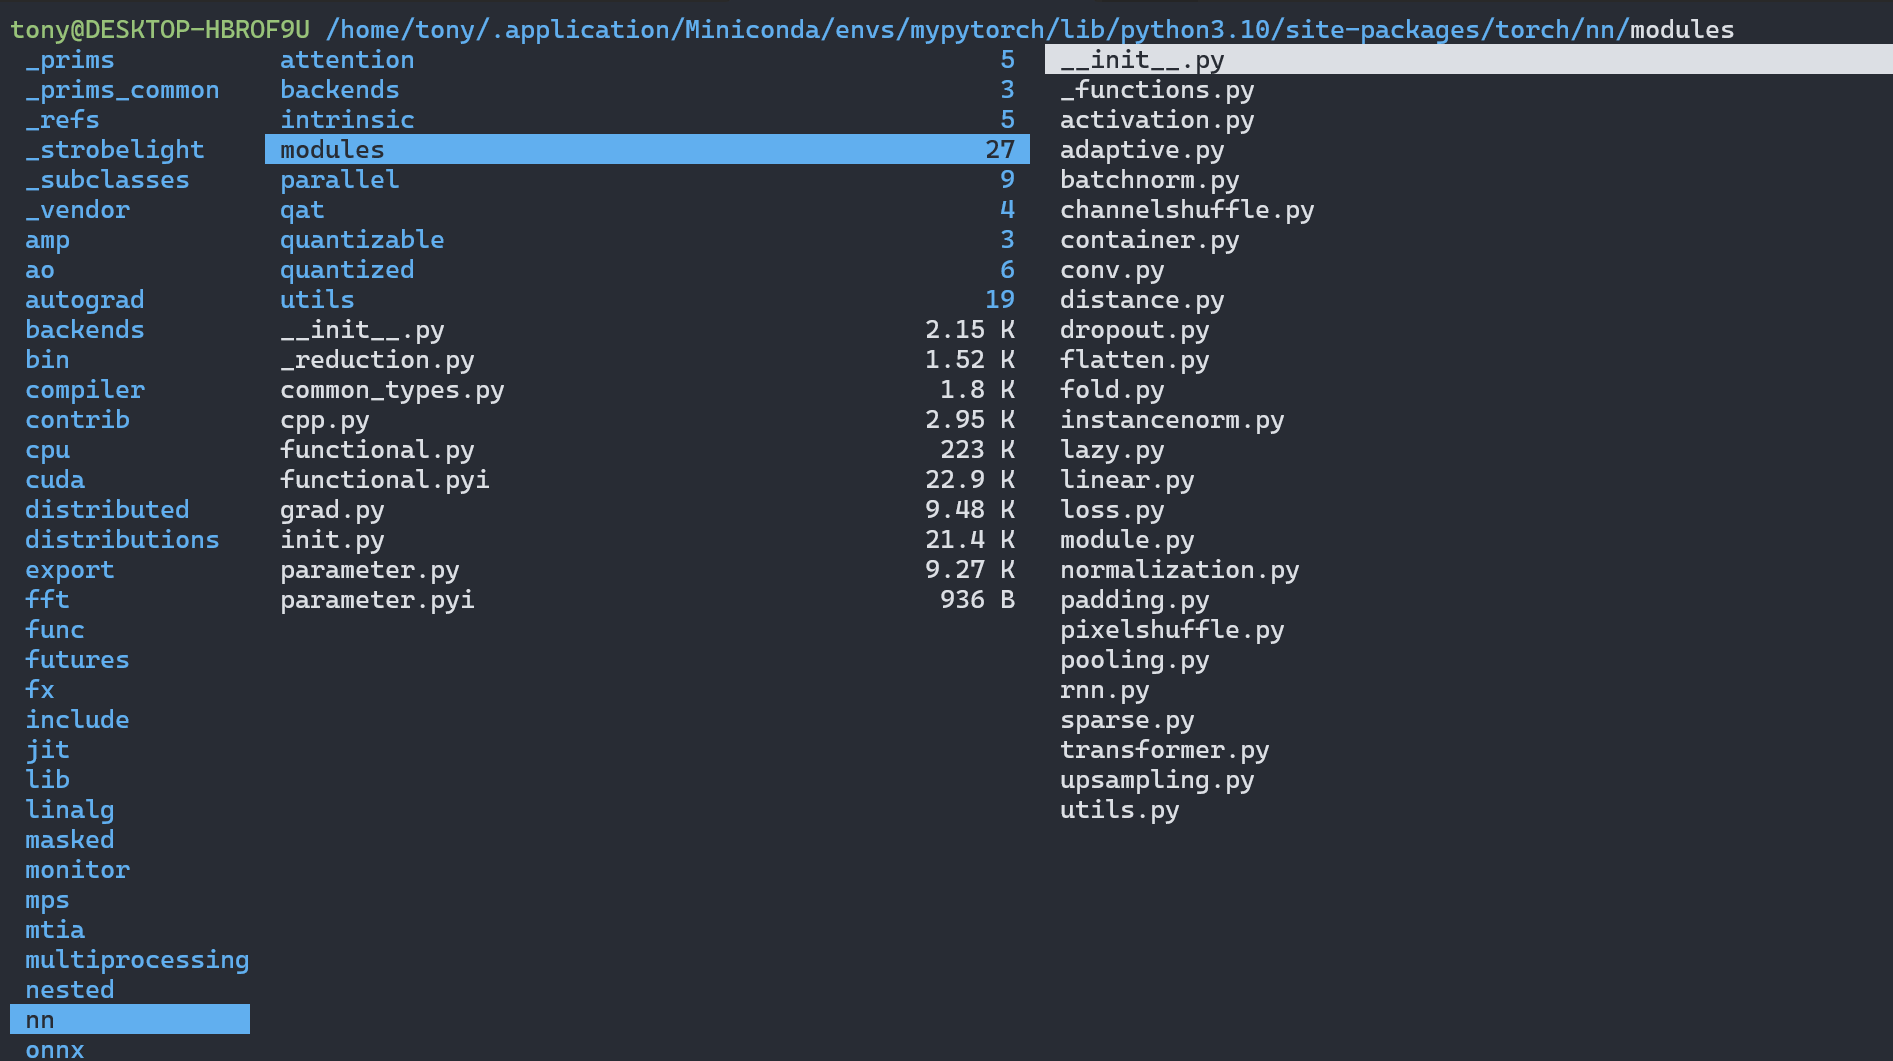
\includegraphics[width=0.6\textwidth]{part/人工智能/深度学习框架/pic/Pytorch/PyTorch概述/nn.modules中的网络层.png}
        \caption{nn.modules中的网络层}
        \label{fig:nn.modules中的网络层}
    \end{figure}
    

    \item onnx
    
    pytorch模型转换到onnx模型表示的核心模块，
    进入文件夹可以看到大量的\codeinline{opset**.py}，

    \item optim
    
    优化模块，深度学习的学习过程，就是不断的优化，而优化使用的方法函数，
    都暗藏在了optim文件夹中，进入该文件夹，
    可以看到熟悉的优化方法：“Adam”、“SGD”、“ASGD”等。以及非常重要的学习率调整模块，\codeinline{lr\_scheduler.py}。
    
    \begin{figure}[htpb]
        \centering
        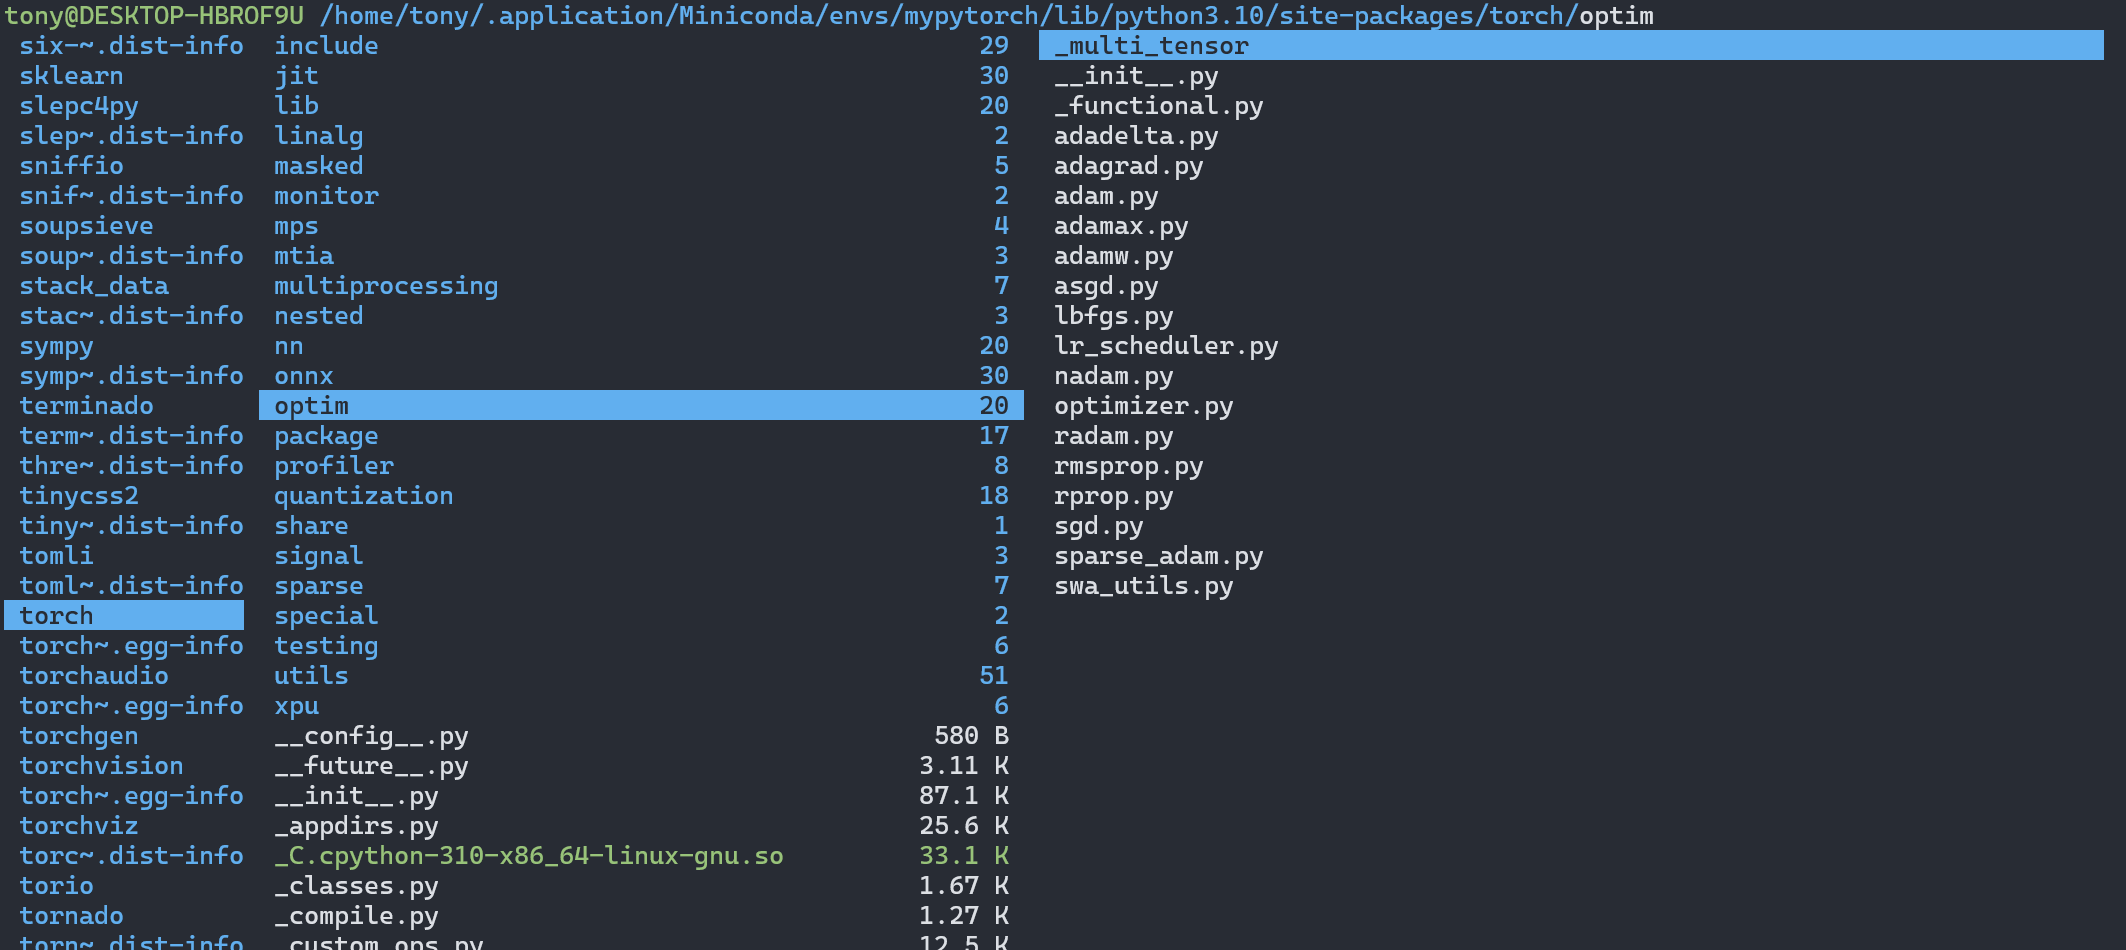
\includegraphics[width=0.6\textwidth]{part/人工智能/深度学习框架/pic/Pytorch/PyTorch概述/optim中的算法.png}
        \caption{optim中的算法}
        \label{fig:optim中的算法}
    \end{figure}
    

    \item utils
    
    utils是各种软件工程中常见的文件夹，其中包含了各类常用工具，
    其中比较关键的是data文件夹，tensorboard文件夹，
    这些工具都将在后续章节详细展开。
\end{enumerate}


\subsection{torchvision 相关}
\label{subsec:torchvision相关}
专门为计算机视觉任务设计的附加库，扩展了 PyTorch 的功能。

\subsubsection{torchvision 安装目录}
\label{subsubsec:torchvision安装目录}
\begin{figure}[htpb]
    \centering
    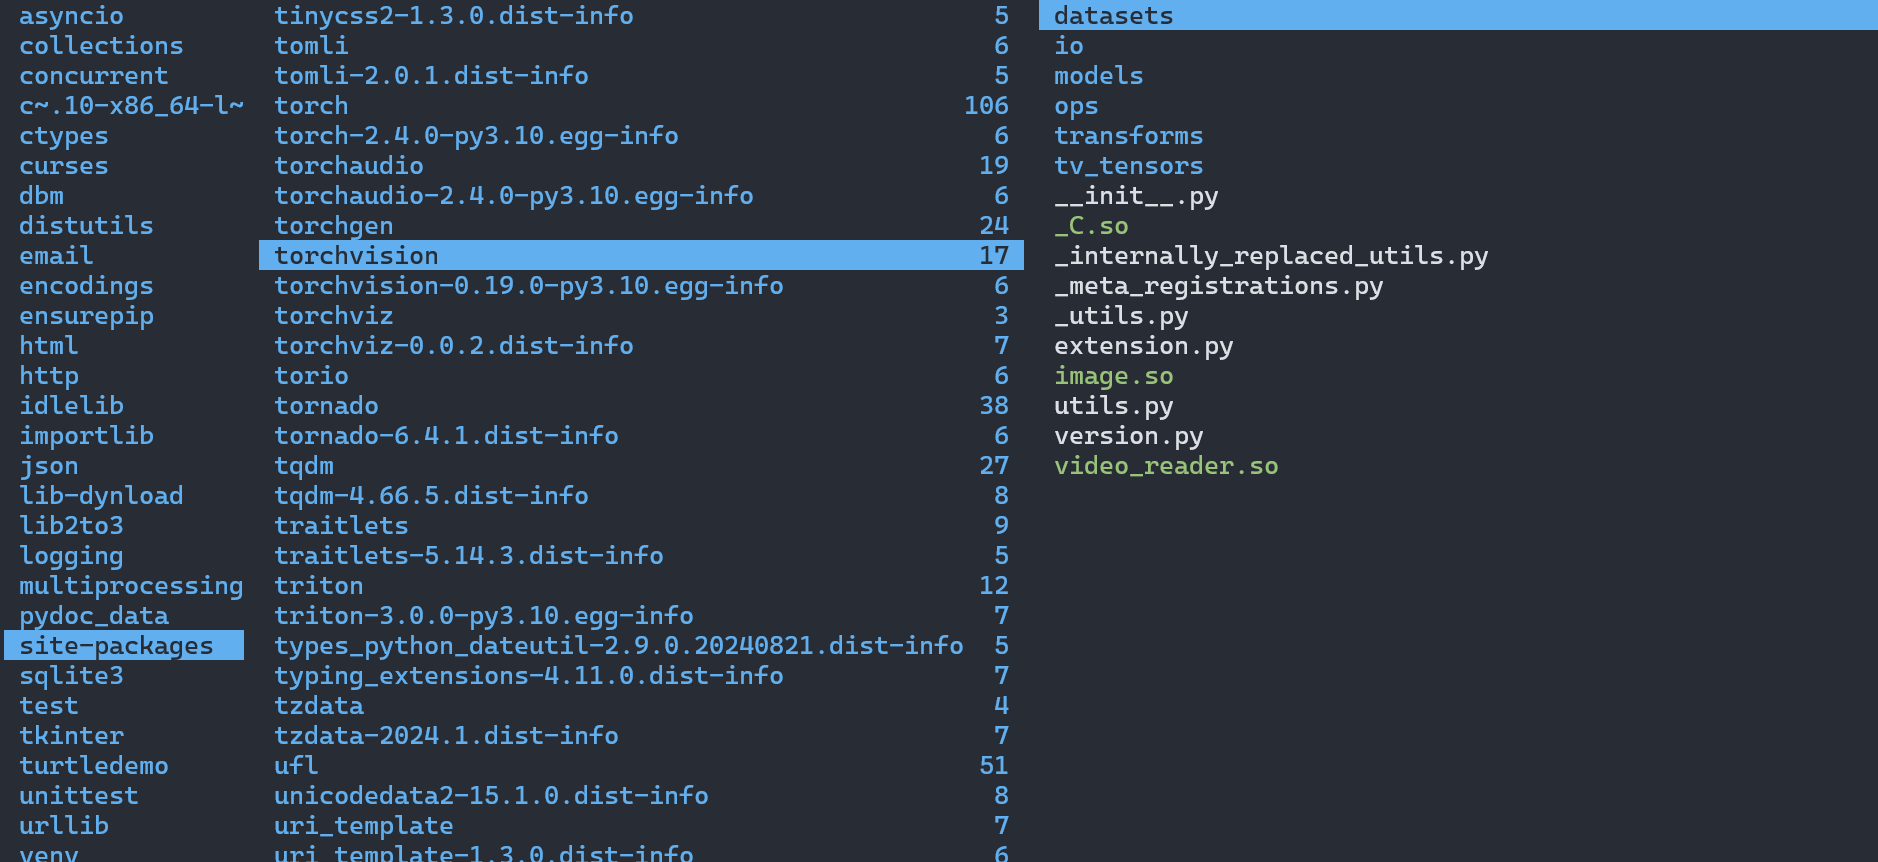
\includegraphics[width=0.6\textwidth]{part/人工智能/深度学习框架/pic/Pytorch/PyTorch概述/torchvision的安装目录.png}
    \caption{torchvision的安装目录}
    \label{fig:torchvision的安装目录}
\end{figure}

\subsubsection{torchvision的主要模块}
\label{subsubsec:torchvision的主要模块}
\begin{enumerate}[label=\arabic*)]
    \item datasets
    
    提供了一系列常用的计算机视觉数据集的接口，如 CIFAR-10、ImageNet、MNIST 等。用户可以通过简单的 API 下载、加载和预处理这些数据集。

    \begin{figure}[htpb]
        \centering
        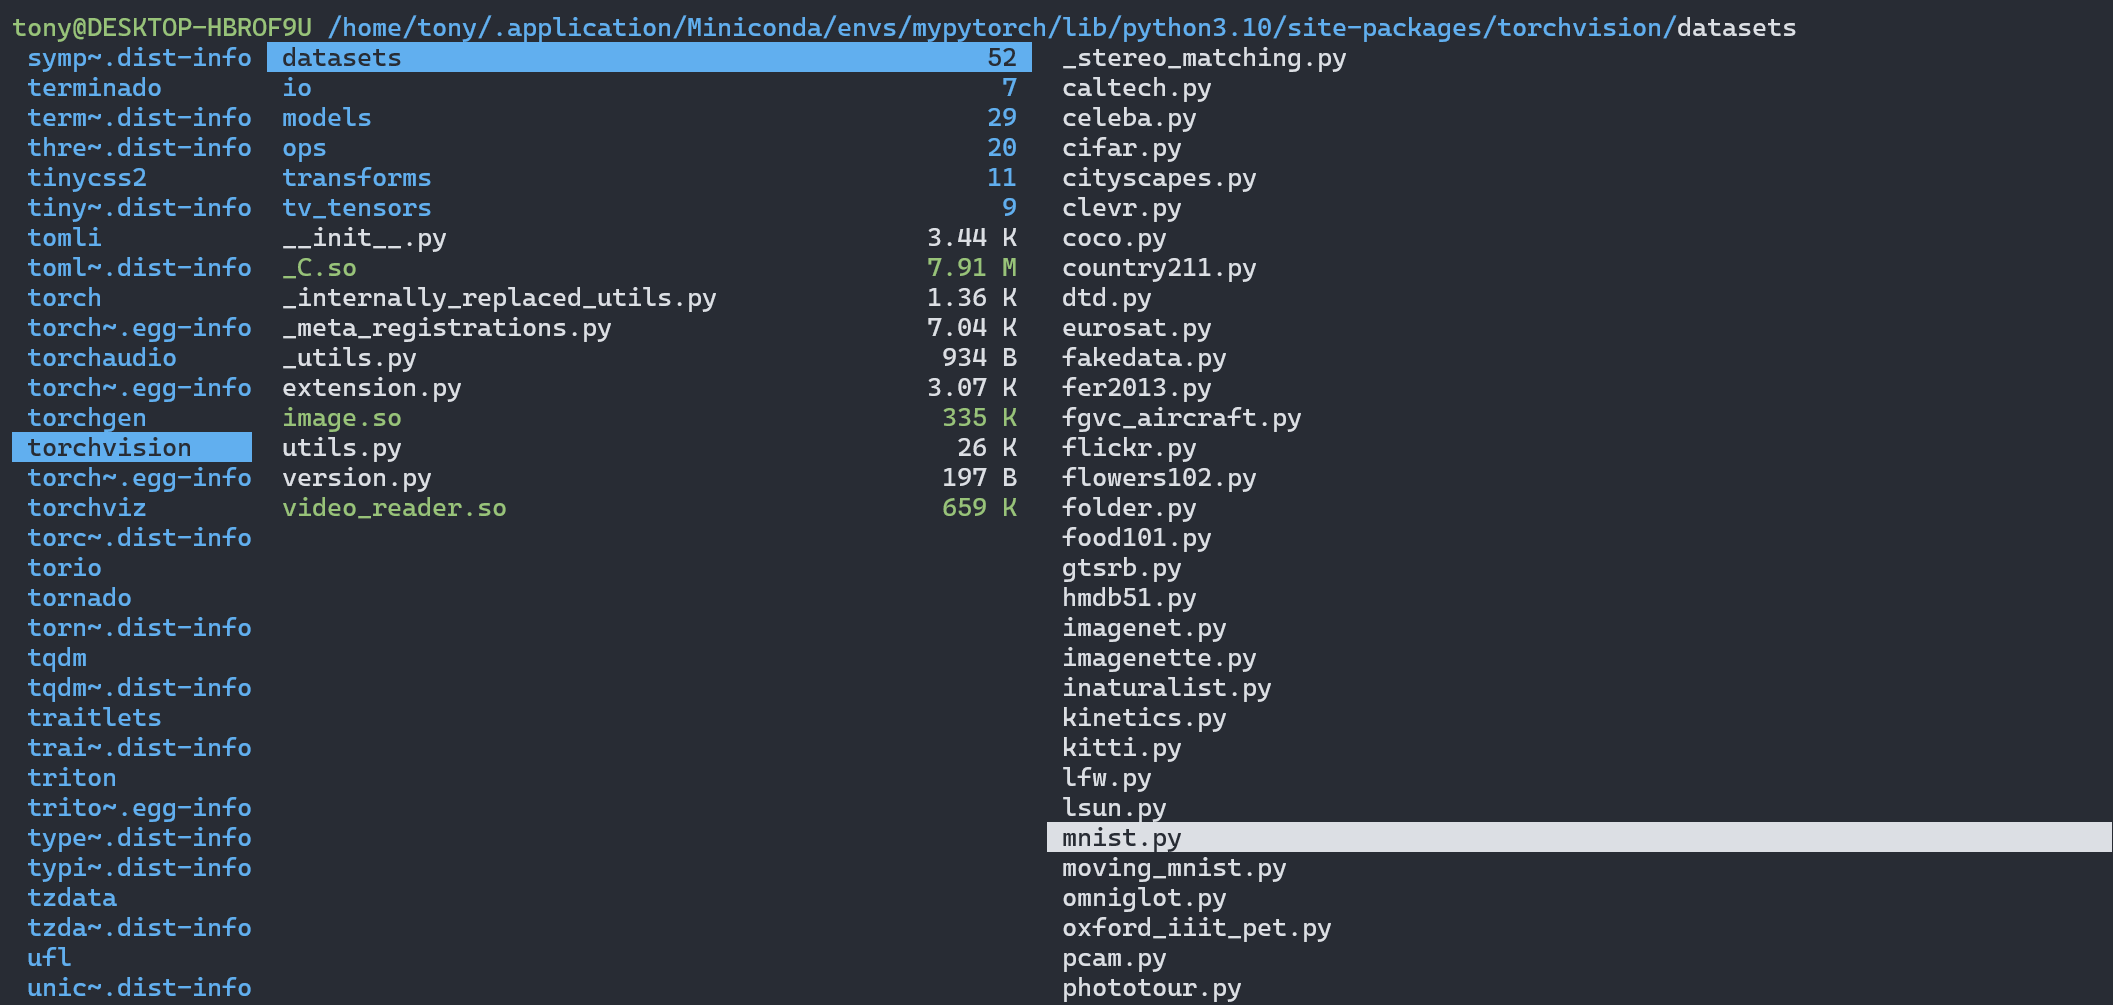
\includegraphics[width=0.6\textwidth]{part/人工智能/深度学习框架/pic/Pytorch/PyTorch概述/datasets内容.png}
        \caption{datasets内容}
        \label{fig:datasets内容}
    \end{figure}
    
    \item models:预训练模型
    
    这里是宝藏库，里边存放了经典的、可复现的、有训练权重参数可下载的视觉模型，
    例如分类的alexnet、densenet、efficientnet、mobilenet-v1/2/3、resnet等，
    分割模型、检测模型、视频任务模型、量化模型。
    

    \item ops
    
    视觉任务特殊的功能函数，例如检测中用到的 roi\_align, roi\_pool，boxes的生成，以及focal\_loss实现，都在这里边有实现。

    \item transforms:图像转换
    
    提供了一系列常用的图像预处理方法。数据增强，数据预处理，数据增强的函数都在这里，
    例如缩放(resize), 裁剪(crop), 归一化(normalize), 旋转(rotate), 翻转(flip)等。

    通过\codeinline{torchvision/transforms/transforms.py}, 可以看到 torchvision包含了这些功能

    \begin{lstlisting}[style=demostyle,numbers=none]
    __all__ = ["Compose", "ToTensor", "PILToTensor", "ConvertImageDtype", "ToPILImage", "Normalize", "Resize", "Scale",
           "CenterCrop", "Pad", "Lambda", "RandomApply", "RandomChoice", "RandomOrder", "RandomCrop",
           "RandomHorizontalFlip", "RandomVerticalFlip", "RandomResizedCrop", "RandomSizedCrop", "FiveCrop", "TenCrop",
           "LinearTransformation", "ColorJitter", "RandomRotation", "RandomAffine", "Grayscale", "RandomGrayscale",
           "RandomPerspective", "RandomErasing", "GaussianBlur", "InterpolationMode", "RandomInvert", "RandomPosterize",
           "RandomSolarize", "RandomAdjustSharpness", "RandomAutocontrast", "RandomEqualize"]
    \end{lstlisting}
\end{enumerate}











\chapter{PyTorch基础}
\section{Tensor概述}
\subsection{Tensor简介}
pytorch的核心数据结构——Tensor（张量）。

Tensor 中文被翻译为张量。张量在不同学科中有不同的意义，
在深度学习中张量表示的是一个多维数组，它是标量、向量、矩阵的拓展。

张量的每一个方向被称为\textcolor{blue}{\textbf{模}}（Mode）。

张量的\textcolor{YBXPurple}{阶数}就是它的\textcolor{YBXPurple}{维数}，
一阶张量就是向量，二阶张量就是矩阵，三阶及其以上的张量统称为高阶张量。

Tensor可以是零维（又称为标量或一个数）、一维(向量)、 二维(矩阵)及多维的数组。

一个RGB图像的数组就是一个三维张量，第一维是图像的高，第二维是图像的宽，第三维是图像的颜色通道。

\subsection{Tensor的作用}
tensor自称为神经网络界的NumPy,它与NumPy的ndarray相似，
二者均可共享内存，且它们之间的转换非常方便和高效。
不过它们也有不同之处，最大的区别就是NumPy会把\codeinline{ndarray}放在CPU中加速运算，而
\codeinline{Tensor}会放在GPU中进行加速运算（假设当前环境有GPU）。

tensor用于表达各类数据，如输入数据、模型的参数、模型的特征图、模型的输出等。
这里边有一个很重要的数据，就是模型的参数。对于模型的参数，我们需要更新它们，
而更新操作需要记录梯度，梯度的记录功能正是被张量所实现的（求梯度是autograd实现的）。

\subsection{torch.Tensor和torch.tensor}
\reminder{\lefthand}{习惯上不区分Tensor和tensor，但主要用小写的tensor表示张量这个数据类型。}
在pytorch中，有两个张量的相关概念极其容易混淆，分别是\codeinline{torch.Tensor} \\
和 \codeinline{torch.tensor}。
        
\textcolor{red}{\textbf{注意}}：\codeinline{torch.Tensor} 和 \codeinline{torch.tensor} 的区别
\begin{enumerate}[label=\arabic*)]
    \item \codeinline{torch.Tensor} 是 \codeinline{torch.tensor} 和 \codeinline{torch.empty} 的一种混合。
    但是当传入数据时，\codeinline{torch.Tensor}使用全局默认数据类型(FloatTensor), 
    \codeinline{torch.tensor}从数据中推断数据类型。

    \item \codeinline{torch.tensor(1)} 是一个标量，而 \codeinline{torch.Tensor(1)}(类似\codeinline{torch.tensor([1])}) 是一个一维张量。

    \item \codeinline{torch.tensor} 函数确实创建了一个 \codeinline{torch.Tensor} 实例，
    但它不是直接调用 \codeinline{torch.Tensor} 类构造函数。
    
    \codeinline{torch.tensor} 是 PyTorch 提供的一个高层次的函数，主要用于将 Python 的数组或列表对象转换为 \codeinline{torch.Tensor} 对象。
\end{enumerate}

其实，通过命名规范，可知道torch.Tensor是Python的一个类, torch.tensor是Python的一个函数。
通常我们调用torch.tensor进行创建张量，而不直接调用torch.Tensor类进行创建。

\begin{lstlisting}[style=pythonstyle]
import torch
tl=torch.Tensor(1)
t2=torch.tensor(1)
t3=torch.tensor([1])
print ("tl 的值{}, tl 的数据类型{} ".format (tl, tl.type()))
print ("t2 的值{}, t2 的数据类型{} ".format (t2, t2.type()))
print ("t3 的值{}, t3 的数据类型{} ".format (t3, t3.type()))
\end{lstlisting}
\begin{lstlisting}[style=demostyle,numbers=none]
tl 的值tensor([-2.5500e-22]), tl 的数据类型torch.FloatTensor 
t2 的值1, t2 的数据类型torch.LongTensor 
t3 的值tensor([1.]), t3 的数据类型torch.FloatTensor 
\end{lstlisting}

\subsection{Tensor的历史演变}
\subsection{Tensor的结构属性}
张量是PyTorch的基本数据结构，在使用时需要表示成\codeinline{torch.Tensor}的形式，
它有8个主要的属性前4个属性与数据相关，后4个属性与梯度求导相关

\begin{enumerate}[label=\arabic*)]
        \item \codeinline{data}:被包装的张量。
        \item \codeinline{dtype}：张量的数据类型。

        如表\ref{tab:张量数据类型}所示，PyTorch中有9种不同的数据类型。
        \begin{table}[h]
        \centering
        \resizebox{0.8\textwidth}{!}{
        \begin{tabular}{|c|c|l|l|}
        \hline
        \textbf{Data Type} & \textbf{dtype} & \textbf{CPU Tensor} & \textbf{GPU Tensor} \\ \hline
        32-bit floating point & \codeinline{torch.float32} or \codeinline{torch.float} & \codeinline{torch.FloatTensor} & \codeinline{torch.cuda.FloatTensor} \\ \hline
        64-bit floating point & \codeinline{torch.float64} or \codeinline{torch.double} & \codeinline{torch.DoubleTensor} & \codeinline{torch.cuda.DoubleTensor} \\ \hline
        16-bit floating point & \codeinline{torch.float16} or \codeinline{torch.half} & \codeinline{torch.HalfTensor} & \codeinline{torch.cuda.HalfTensor} \\ \hline
        8-bit integer (unsigned) & \codeinline{torch.uint8} & \codeinline{torch.ByteTensor} & \codeinline{torch.cuda.ByteTensor} \\ \hline
        8-bit integer (signed) & \codeinline{torch.int8} & \codeinline{torch.CharTensor} & \codeinline{torch.cuda.CharTensor} \\ \hline
        16-bit integer (signed) & \codeinline{torch.int16} or \codeinline{torch.short} & \codeinline{torch.ShortTensor} & \codeinline{torch.cuda.ShortTensor} \\ \hline
        32-bit integer (signed) & \codeinline{torch.int32} or \codeinline{torch.int} & \codeinline{torch.IntTensor} & \codeinline{torch.cuda.IntTensor} \\ \hline
        64-bit integer (signed) & \codeinline{torch.int64} or \codeinline{torch.long} & \codeinline{torch.LongTensor} & \codeinline{torch.cuda.LongTensor} \\ \hline
        Boolean & \codeinline{torch.bool} & \codeinline{torch.BoolTensor} & \codeinline{torch.cuda.BoolTensor} \\ \hline
        \end{tabular}
        }
        \caption{张量数据类型}
        \label{tab:张量数据类型}
        \end{table}

        \item \codeinline{shape}：张量的形状/维度。
        \item \codeinline{device}:张量所在设备，加速计算的关键，GPU或CPU。

        \item \codeinline{grad}: data的梯度。
        \item \codeinline{grad\_fn}：创建张量的函数，这是自动求导的关键。
        \item \codeinline{requires\_grad}:指示是否需要计算梯度。
        \item \codeinline{is\_leaf}：指示是否是叶子节点。
\end{enumerate}

\section{Tensor操作}
\subsection{Tensor操作分类}
对Tensor的操作很多，从接口的角度来划分，可以分为两类：
\begin{enumerate}[label=\arabic*)]
    \item \codeinline{torch.function} 接口中的函数是PyTorch的全局函数，通常用于创建、操作、转换和计算张量。这些函数通常以张量作为输入并返回新的张量。
    \begin{enumerate}[itemindent=1em,label=\arabic*)]
        \item \codeinline{torch.tensor(data)}: 从\codeinline{data}创建一个\codeinline{Tensor}。
        \item \codeinline{torch.zeros(size)}: 创建一个大小为\codeinline{size}的全0张量。
        \item \codeinline{torch.ones(size)}: 创建一个大小为\codeinline{size}的全1张量。
        \item \codeinline{torch.rand(size)}: 创建一个大小为\codeinline{size}的随机张量。
        \item \codeinline{torch.arange(start, end, step)}: 创建一个从\codeinline{start}到\codeinline{end}，步长为\codeinline{step}的张量。
        \item \codeinline{torch.add(tensor1, tensor2)}: 将两个张量相加。
        \item \codeinline{torch.sub(tensor1, tensor2)}: 将两个张量相减。
        \item \codeinline{torch.mul(tensor1, tensor2)}: 将两个张量相乘。
        \item \codeinline{torch.div(tensor1, tensor2)}: 将两个张量相除。
        \item \codeinline{torch.pow(tensor1, tensor2)}: 将\codeinline{tensor1}的\codeinline{tensor2}次方。
        \item \codeinline{torch.sqrt(tensor)}: 计算\codeinline{tensor}的
        \item \codeinline{torch.exp(tensor)}: 计算\codeinline{tensor}的指数。
        \item \codeinline{torch.log(tensor)}: 计算\codeinline{tensor}的对数。
        \item \codeinline{torch.sin(tensor)}: 计算\codeinline{tensor}的正弦。
        \item \codeinline{torch.cos(tensor)}: 计算\codeinline{tensor}的余弦。
        \item \codeinline{torch.tan(tensor)}: 计算\codeinline{tensor}的正切。
        \item \codeinline{torch.sigmoid(tensor)}: 计算\codeinline{tensor}的Sigmoid函数。
        \item \codeinline{torch.relu(tensor)}: 计算\codeinline{tensor}的ReLU函数。
        \item \codeinline{torch.max(tensor)}: 计算\codeinline{tensor}的最大值。
        \item \codeinline{torch.min(tensor)}: 计算\codeinline{tensor}的最小值。
        \item \codeinline{torch.mean(tensor)}: 计算\codeinline{tensor}的平均值。
        \item \codeinline{torch.sum(tensor)}: 计算\codeinline{tensor}的和。
        \item \codeinline{torch.dot(tensor1, tensor2)}: 计算\codeinline{tensor1}和\codeinline{tensor2}的点积。
        \item \codeinline{torch.mm(tensor1, tensor2)}: 计算\codeinline{tensor1}和\codeinline{tensor2}的矩阵乘法。
        \item \codeinline{torch.cat(tensor1, tensor2)}: 沿着指定维度拼接张量。
        \item \codeinline{torch.stack(tensor1, tensor2)}: 沿着新维度拼接张量。
        \item \codeinline{torch.reshape(tensor, shape)}: 改变张量的形状。
    \end{enumerate}
    
    \item \codeinline{tensor.function} 接口是张量对象的方法，这些方法直接作用于张量本身。它们通常是 \codeinline{torch.function} 接口的实例方法版本。
    \begin{enumerate}[itemindent=1em,label=\arabic*)]
        \item \codeinline{tensor.item()}: 将张量转换为标量。
        \item \codeinline{tensor.numpy()}: 将张量转换为NumPy数组。
        \item \codeinline{tensor.to(device)}: 将张量移动到指定设备。
        \item \codeinline{tensor.cpu()}: 将张量移动到CPU。
        \item \codeinline{tensor.cuda()}: 将张量移动到GPU。
        \item \codeinline{tensor.add(tensor)}: 将两个张量相加。
        \item \codeinline{tensor.sub(tensor)}: 将两个张量相减。
        \item \codeinline{tensor.mul(tensor)}: 将两个张量相乘。
        \item \codeinline{tensor.div(tensor)}: 将两个张量相除。
        \item \codeinline{tensor.pow(tensor)}: 将\codeinline{tensor}的\codeinline{tensor}次方。
        \item \codeinline{tensor.sqrt()}: 计算\codeinline{tensor}的平方根。
        \item \codeinline{tensor.exp()}: 计算\codeinline{tensor}的指数。
        \item \codeinline{tensor.log()}: 计算\codeinline{tensor}的对数。
        \item \codeinline{tensor.transpose(dim1, dim2)}: 交换张量的两个维度。
        \item \codeinline{tensor.t()}: 转置张量。
        \item \codeinline{tensor.transpose(dim1, dim2)}: 交换张量的两个维度。
        \item \codeinline{tensor.view(shape)}: 改变张量的形状。
    \end{enumerate}
\end{enumerate}

\subsection{创建Tensor}
如表\ref{tab:Pytorch创建Tensor的函数}所示，PyTorch提供了很多创建张量的函数。

\begin{table}[h]
	\centering
	\resizebox{0.8\textwidth}{!}{
	\begin{tabular}{|l|l|}
	\hline
	\textbf{函数} & \textbf{功能} \\ \hline
	\codeinline{Tensor(*size)} & 直接从参数创建一个张量，支持 \codeinline{list}、\codeinline{numpy} 数组 \\ \hline
	\codeinline{eye(row, column)} & 创建指定行数、列数的二维单位张量 \\ \hline
	\codeinline{linspace(start, end, steps)} & 从 \codeinline{start} 到 \codeinline{end}，均匀切分成 \codeinline{steps} 份 \\ \hline
	\codeinline{logspace(start, end, steps)} & 从 \(10^{\text{start}}\) 到 \(10^{\text{end}}\)，均匀切分成 \codeinline{steps} 份 \\ \hline
	\codeinline{rand/randn(*size)} & 生成 \([0, 1]\) 均匀分布/标准正态分布数据 \\ \hline
	\codeinline{ones(*size)} & 返回指定形状的张量，元素初始为 1 \\ \hline
	\codeinline{zeros(*size)} & 返回指定形状的张量，元素初始为 0 \\ \hline
	\codeinline{ones\_like(t)} & 返回与 \codeinline{t} 形状相同的张量，且元素初始为 1 \\ \hline
	\codeinline{zeros\_like(t)} & 返回与 \codeinline{t} 形状相同的张量，且元素初始为 0 \\ \hline
	\codeinline{arange(start, end, step)} & 在区间 \codeinline{[start, end]} 上以间隔 \codeinline{step} 生成一个序列张量 \\ \hline
	\codeinline{from\_numpy(ndarray)} & 把 \codeinline{ndarray} 转换为 Tensor \\ \hline
	\end{tabular}}
	\caption{常见的创建 Tensor 的函数}
	\label{tab:Pytorch创建Tensor的函数}
\end{table}

如果分类的话，创建张量的方式可以分为以下几种：

\subsubsection{直接创建}
通过\codeinline{torch.tensor}创建张量

\begin{lstlisting}[style=demostyle,numbers=none]
torch.tensor(data, dtype=None, device=None, requires_grad=False, pin_memory=False)
# data: 数据
#     PyTorch 支持通过list、 tuple、numpy array、scalar 等多种类型进行数据传入，
#     并转换为 tensor。
# dtype: 张量数据类型
# device: 存放设备
# requires_grad: 是否需要梯度
#      只有当一个 Tensor 设置 requires_grad 为 True 的情况下，
#      才会对这个 Tensor 以及由这个 Tensor 计算出来的其他 Tensor 进行求导，
#      然后将导数值存在Tensor 的 grad 属性中，便于优化器来更新参数。
#      
#      依赖于叶子节点的节点，requires_grad 默认为 True
#
#   如果是训练过程就要设置为 true，目的是方便求导、更新参数。
#   而到了验证或者测试过程，我们的目的是检查当前模型的泛化能力，
#   那就要把 requires_grad 设置成 Fasle，避免这个参数根据 loss 自动更新
# pin_memory: 是否存放在锁页内存，以加速数据传输。
#      在GPU上，如果数据存放在锁页内存中，那么GPU的显存占用会更少，
#      从而可以更快的进行运算。
\end{lstlisting}

\begin{lstlisting}[style=pythonstyle]
import torch
a = torch.tensor([1,2,3], dtype=torch.float32)

b = torch.tensor([[1,2,3],[4,5,6]], 
                dtype=torch.float32,
                device=torch.device('cuda:0'), # 存放在第一个GPU上
                requires_grad=True,
                pin_memory=True
                )
\end{lstlisting}





\subsubsection{从NumPy数组创建}
\begin{lstlisting}[style=demostyle,numbers=none]
# 功能: 从 numpy 数组创建张量
torch.from_numpy(ndarray)
\end{lstlisting}

\begin{lstlisting}[style=pythonstyle]
import numpy as np
a = np.zeros(3)

b = torch.from_numpy(a)
\end{lstlisting}

\textcolor{red}{\textbf{注意}}:从\codeinline{torch.from\_numpy()}创建的张量和原始的\codeinline{ndarray}共享内存，修改其中一个，另一个也会改变。
\begin{lstlisting}[style=pythonstyle]
import numpy as np
import torch
arr = np.array([[1, 2, 3], [4, 5, 6]])
print("arr: ", arr)
t = torch.from_numpy(arr)
print("t: ", t)

print("\n修改arr")
arr[0, 0] = 0
print("arr: ", arr)
print("t: ", t)
\end{lstlisting}
\begin{lstlisting}[style=demostyle,numbers=none]
arr:  [[1 2 3]
        [4 5 6]]
t:  tensor([[1, 2, 3],
        [4, 5, 6]])

修改arr
arr:  [[0 2 3]
        [4 5 6]]
t:  tensor([[0, 2, 3],
        [4, 5, 6]]) 
\end{lstlisting}  

\subsubsection{概率分布创建张量}
\begin{enumerate}[label=\arabic*)]
\item 从正态分布(高斯分布)中抽取随机数创建张量
\begin{lstlisting}[style=demostyle,numbers=none]
torch.normal(size, mean, std)   # 指定均值和标准差的正态分布
# size: 仅在mean和std均为标量时使用，表示创建张量的形状。
# mean: 正态分布的均值
# std: 正态分布的标准差
\end{lstlisting}
\begin{lstlisting}[style=pythonstyle,mathescape=true]
import torch

mean = torch.arange(1, 5, dtype=torch.float)
std = torch.arange(1, 5, dtype=torch.float)
# 将会为每一对 mean_i 和 std_i 生成一个服从正态分布的随机数 t_i。
# 每次运行的结果都不一样。
# $\textcolor{DarkGreen}{t_0}$: 生成一个随机数 $\textcolor{DarkGreen}{t_0}$，服从 $\textcolor{DarkGreen}{N(1.0, 1.0^2)}$。
# $\textcolor{DarkGreen}{t_1}$: 生成一个随机数 $\textcolor{DarkGreen}{t_1}$，服从 $\textcolor{DarkGreen}{N(2.0, 2.0^2)}$。
t = torch.normal(mean, std)
print("mean:{}\nstd:{}\n{}".format(mean, std, t))

print("-----------------------------")
# mean是一个张量，std是一个标量
t = torch.normal(mean, 1.0)
print("mean:{}\nstd:{}\n{}".format(mean, 1.0, t))

print("-----------------------------")
# mean是一个标量，std是一个张量
t = torch.normal(0.0, std)
print("mean:{}\nstd:{}\n{}".format(0.0, std, t))

print("-----------------------------")
# mean和std都是标量，size指定张量的形状
t = torch.normal(mean=0.0, std=1.0, size=(4,))
print("mean:{}\nstd:{}\n{}".format(mean, std, t))
\end{lstlisting}
\begin{lstlisting}[style=demostyle,numbers=none]
$ python3 test.py
mean:tensor([1., 2., 3., 4.])
std:tensor([1., 2., 3., 4.])
tensor([1.9618, 3.5882, 2.0549, 3.7797])
-----------------------------
mean:tensor([1., 2., 3., 4.])
std:1.0
tensor([0.1122, 0.2529, 2.5417, 4.8538])
-----------------------------
mean:0.0
std:tensor([1., 2., 3., 4.])
tensor([-0.2920, -0.8096, -4.0819, -2.9697])
-----------------------------
mean:tensor([1., 2., 3., 4.])
std:tensor([1., 2., 3., 4.])
tensor([-0.8268, -0.1924, -0.1457, -1.2918])

$ python3 test.py        
mean:tensor([1., 2., 3., 4.])
std:tensor([1., 2., 3., 4.])
tensor([1.9121, 0.8003, 5.2724, 3.5752])
-----------------------------
mean:tensor([1., 2., 3., 4.])
std:1.0
tensor([-0.4556,  3.1790,  0.8509,  3.6606])
-----------------------------
mean:0.0
std:tensor([1., 2., 3., 4.])
tensor([-0.0166,  1.5871,  3.0519,  1.8443])
-----------------------------
mean:tensor([1., 2., 3., 4.])
std:tensor([1., 2., 3., 4.])
tensor([-0.8179, -0.5369,  0.3769,  1.6214])
\end{lstlisting}

\item 从标准正态分布中抽取随机数创建张量
\begin{lstlisting}[style=demostyle,numbers=none]
torch.randn(size,        # 数据类型为浮点型且维度指定
                out=None,    # 输出张量
                dtype=None,  # 数据类型
                layout=torch.strided, # 默认为默认布局
                device=None, # 设备
                requires_grad=False)  # 是否需要梯度
# 数据类型为浮点型且维度指定,随机数满足均值为 0、方差为 1标准正态分布

torch.randn_like(input,  # 生成一个与 input 形状相同的张量
                        dtype=None,  # 数据类型
                        layout=None, # 默认为默认布局
                        device=None, # 默认为当前设备
                        requires_grad=False)  # 是否需要梯度
# 生成一个与 input 形状相同的张量，随机数满足均值为 0、方差为 1标准正态分布
\end{lstlisting}
\begin{lstlisting}[style=pythonstyle]
# randn(*size)
import torch
randn_tensor = torch.randn(2, 2)
print("\nrandn(*size):")
print("Shape:", randn_tensor.shape)
print("Content:\n", randn_tensor)

# randn_like(input)
randn_like_tensor = torch.randn_like(randn_tensor)
print("\nrandn_like(input):")
print("Shape:", randn_like_tensor.shape)
print("Content:\n", randn_like_tensor)
\end{lstlisting}
\begin{lstlisting}[style=demostyle,numbers=none]
$> python3 test.py
randn(*size):
Shape: torch.Size([2, 2])
Content:
tensor([[-0.5008,  1.1298],
        [ 0.7826,  0.1865]])

randn_like(input):
Shape: torch.Size([2, 2])
Content:
tensor([[ 0.0411, -0.9603],
        [-1.4047, -1.2398]])

$> python3 test.py
randn(*size):
Shape: torch.Size([2, 2])
Content:
tensor([[-0.9106,  0.6807],
        [-0.1289, -0.5300]])

randn_like(input):
Shape: torch.Size([2, 2])
Content:
tensor([[-0.2527, -0.8041],
        [ 0.9786,  2.0623]])
\end{lstlisting}

\item 从0-1均匀分布中抽取随机数创建张量
\begin{lstlisting}[style=demostyle,numbers=none]
# 数据类型为浮点型且维度指定
torch.rand(size,        # 数据类型为浮点型且维度指定
                out=None,    # 输出张量
                dtype=None,  # 数据类型
                device=None, # 设备
                requires_grad=False)  # 是否需要梯度

# 生成一个与 input 形状相同的张量
torch.rand_like(input,  # 生成一个与 input 形状相同的张量
                        dtype=None,  # 数据类型
                        layout=None, # 默认为默认布局
                        device=None, # 默认为当前设备
                        requires_grad=False)  # 是否需要梯度
\end{lstlisting}
\begin{lstlisting}[style=pythonstyle]
# rand(*size)
import torch
rand_tensor = torch.rand(2, 2)
print("\nrand(*size):")
print("Shape:", rand_tensor.shape)
print("Content:\n", rand_tensor)

# rand_like(input)
rand_like_tensor = torch.rand_like(rand_tensor)
print("\nrand_like(input):")
print("Shape:", rand_like_tensor.shape)
print("Content:\n", rand_like_tensor)
\end{lstlisting}
\begin{lstlisting}[style=demostyle,numbers=none]
$> python3 test.py
rand(*size):
Shape: torch.Size([2, 2])
Content:
tensor([[0.6926, 0.4433],
        [0.3605, 0.7165]])

rand_like(input):
Shape: torch.Size([2, 2])
Content:
tensor([[0.5039, 0.9240],
        [0.8755, 0.7009]])

$> python3 test.py
rand(*size):
Shape: torch.Size([2, 2])
Content:
tensor([[0.7404, 0.5186],
        [0.6042, 0.0406]])

rand_like(input):
Shape: torch.Size([2, 2])
Content:
tensor([[0.4726, 0.9517],
        [0.9636, 0.8840]])
\end{lstlisting}

\begin{lstlisting}[style=demostyle,numbers=none]
# 同 torch.rand(size)  只不过得到的是整数随机数
torch.randint(low=0,    # 生成的随机数下界
                high,     # 生成的随机数上界
                size，    # 张量的形状
                out=None, # 输出张量
                dtype=None,   # 数据类型
                layout=None,  # 默认为默认布局
                device=None,  # 默认为当前设备
                requires_grad=False)  # 是否需要梯度

# 生成一个与 input 形状相同的张量
torch.randint_like(input,  # 输入张量
                        low,    # 生成的随机数下界
                        high,   # 生成的随机数上界
                        dtype=None,   # 数据类型
                        layout=None,  # 默认为默认布局
                        device=None,  # 默认为当前设备
                        requires_grad=False)  # 是否需要梯度
\end{lstlisting}
\begin{lstlisting}[style=pythonstyle]
import torch

# randint(low, high, *size)
rand_tensor = torch.randint(low=3, high=10, size=(2, 3))
print("\nrand(*size):")
print("Shape:", rand_tensor.shape)
print("Content:\n", rand_tensor)

print("-----------------------------")
# randint_like(input)
rand_like_tensor = torch.randint_like(low=5, high=10, input=rand_tensor)
print("\nrand_like(input):")
print("Shape:", rand_like_tensor.shape)
print("Content:\n", rand_like_tensor)
\end{lstlisting} 
\begin{lstlisting}[style=demostyle,numbers=none]
rand(*size):
Shape: torch.Size([2, 3])
Content:
tensor([[7, 6, 9],
        [8, 7, 9]])
-----------------------------

rand_like(input):
Shape: torch.Size([2, 3])
Content:
tensor([[5, 7, 7],
        [8, 7, 7]])
\end{lstlisting}

\item 生成从0到n-1的随机排列
\begin{lstlisting}[style=demostyle,numbers=none]
torch.randperm(n,       # 生成的随机排列的长度
                out=None, # 输出张量
                dtype=None,   # 数据类型
                layout=torch.strided,  # 默认为默认布局
                device=None,  # 默认为当前设备
                requires_grad=False)  # 是否需要梯度
\end{lstlisting}
\begin{lstlisting}[style=pythonstyle]
import torch

# randperm(n)
randperm_tensor = torch.randperm(10)
print("\nrandperm(n):")
print("Shape:", randperm_tensor.shape)
print("Content:\n", randperm_tensor)
\end{lstlisting}
\begin{lstlisting}[style=demostyle,numbers=none]
randperm(n):
Shape: torch.Size([10])
Content:
        tensor([6, 2, 1, 0, 3, 4, 5, 7, 8, 9])
\end{lstlisting}

\item 生成以input为概率，生成伯努利分布(0-1分布，两点分布)的随机数
\begin{lstlisting}[style=demostyle,numbers=none]
torch.bernoulli(input,  # 输入张量
                out=None, # 输出张量
                generator=None)  # 生成器
\end{lstlisting}
\begin{lstlisting}[style=pythonstyle]
import torch

# bernoulli(input)
bernoulli_tensor = torch.bernoulli(torch.tensor([[0.2, 0.8],[0.5, 0.5]]))
print("\nbernoulli(input):")
print("Shape:", bernoulli_tensor.shape)
print("Content:\n", bernoulli_tensor)
\end{lstlisting}
\begin{lstlisting}[style=demostyle,numbers=none]
bernoulli(input):
Shape: torch.Size([2, 2])
Content:
tensor([[0., 1.],
        [0., 0.]])
\end{lstlisting}

\item 生成一个空张量
\begin{lstlisting}[style=demostyle,numbers=none]
torch.empty(size)   # 随机初始化
\end{lstlisting}
\begin{lstlisting}[style=pythonstyle]
import torch

# empty(*size)
empty_tensor = torch.empty(2, 2)
print("\nempty(*size):")
print("Shape:", empty_tensor.shape)
print("Content:\n", empty_tensor)
\end{lstlisting}
\end{enumerate}
    
\subsubsection{根据数值创建Tensor}                
\label{subsubsec:Pytorch根据数值创建Tensor}
\begin{enumerate}[label=\arabic*)]
\item 创建全0张量
\begin{lstlisting}[style=demostyle,numbers=none]
torch.zeros(size, out, layout, device, requires_grad)   # 全0
# size 张量的形状
# out 输出张量
# layout 布局有strided、sparse_coo、mkldnn、sparse_csr、sparse_csc        
#       strided: 一般的张量
#       sparse_coo: COO格式的稀疏张量
#       mkldnn: MKL-DNN格式的张量
#       sparse_csr: CSR格式的稀疏张量
#       sparse_csc: CSC格式的稀疏张量
# device 设备，如cpu、cuda、cuda:0、cpu:0
# requires_grad 是否需要梯度
\end{lstlisting}
\begin{lstlisting}[style=pythonstyle]
import torch

zeros_tensor = torch.zeros(2, 2) # 创建一个2x2的全0张量
print("\nzeros(*size):")
print("Shape:", zeros_tensor.shape)
print("Content:\n", zeros_tensor)
\end{lstlisting}
\begin{lstlisting}[style=demostyle,numbers=none]
$> python3 test.py
zeros(*size):
Shape: torch.Size([2, 2])
Content:
tensor([[0., 0.],
        [0., 0.]])
\end{lstlisting}

其中\codeinline{out}类似C++中的引用，可以直接修改原来的张量。
\begin{lstlisting}[style=pythonstyle]
import torch
out_t =torch.tensor([2])
print(out_t)
zeros_tensor = torch.zeros(3, 2, out=out_t)

print("zeros_tensor Shape:", zeros_tensor.shape)
print("zeros_tensor Content:\n", zeros_tensor)
print("zeros_tensor id", id(zeros_tensor))
print("-----------------------------")
print("out_t Shape:", out_t.shape)
print("out_t Content:\n", out_t)
print("out_t id", id(out_t))
print("out_t ?= zeros_tensor:", out_t is zeros_tensor)
\end{lstlisting}
\begin{lstlisting}[style=demostyle,numbers=none]
$> python3 test.py
tensor([2])
zeros_tensor Shape: torch.Size([3, 2])
zeros_tensor Content:
tensor([[0, 0],
        [0, 0],
        [0, 0]])
zeros_tensor id 140167783140704
-----------------------------
out_t Shape: torch.Size([3, 2])
out_t Content:
tensor([[0, 0],
        [0, 0],
        [0, 0]])
out_t id 140167783140704

out_t ?= zeros_tensor: True
\end{lstlisting}  
\begin{lstlisting}[style=demostyle,numbers=none]
torch.zeros_like(input, dtype=None, layout=None, device=None, requires_grad=False)   # 全0
# input 输入张量
# dtype 数据类型
# layout 布局有strided、sparse_coo、mkldnn、sparse_csr、sparse_csc        
#       strided: 一般的张量
#       sparse_coo: COO格式的稀疏张量
#       mkldnn: MKL-DNN格式的张量
#       sparse_csr: CSR格式的稀疏张量
#       sparse_csc: CSC格式的稀疏张量
# device 设备，如cpu、cuda、cuda:0、cpu:0
# requires_grad 是否需要梯度
\end{lstlisting}       
\begin{lstlisting}[style=pythonstyle]
import torch

zeros_like_tensor = torch.zeros_like(torch.tensor([2]))
print("\nzeros_like(input):")
print("Shape:", zeros_like_tensor.shape)
print("Content:\n", zeros_like_tensor)
\end{lstlisting}
\begin{lstlisting}[style=demostyle,numbers=none]
$> python3 test.py
zeros_like(input):
Shape: torch.Size([2])
Content:
tensor([0., 0.])
\end{lstlisting}      

\item 创建全1张量
\begin{lstlisting}[style=demostyle,numbers=none]
torch.ones(size, out, layout, device, requires_grad)   # 全1
# size 张量的形状
# out 输出张量
# layout 布局有strided、sparse_coo、mkldnn、sparse_csr、sparse_csc        
#       strided: 一般的张量
#       sparse_coo: COO格式的稀疏张量
#       mkldnn: MKL-DNN格式的张量
#       sparse_csr: CSR格式的稀疏张量
#       sparse_csc: CSC格式的稀疏张量
# device 设备，如cpu、cuda、cuda:0、cpu:0
# requires_grad 是否需要梯度
\end{lstlisting}
\begin{lstlisting}[style=demostyle,numbers=none]
torch.ones_like(input, dtype=None, layout=None, device=None, requires_grad=False)   # 全1
# input 输入张量
# dtype 数据类型
# layout 布局有strided、sparse_coo、mkldnn、sparse_csr、sparse_csc        
#       strided: 一般的张量
#       sparse_coo: COO格式的稀疏张量
#       mkldnn: MKL-DNN格式的张量
#       sparse_csr: CSR格式的稀疏张量
#       sparse_csc: CSC格式的稀疏张量
# device 设备，如cpu、cuda、cuda:0、cpu:0
# requires_grad 是否需要梯度
\end{lstlisting}
\begin{lstlisting}[style=pythonstyle]
import torch
# ones(*size)
ones_tensor = torch.ones(2, 2)
print("\nones(*size):")
print("Shape:", ones_tensor.shape)
print("Content:\n", ones_tensor)

# ones_like(t)
ones_like_tensor = torch.ones_like(tensor)
print("\nones_like(t):")
print("Shape:", ones_like_tensor.shape)
print("Content:\n", ones_like_tensor)
\end{lstlisting}
\begin{lstlisting}[style=demostyle,numbers=none]
$> python3 test.py
ones(*size):
Shape: torch.Size([2, 2])
Content:
tensor([[1., 1.],
        [1., 1.]])

ones_like(t):
Shape: torch.Size([2, 2])
Content:
tensor([[1., 1.],
        [1.,1.]])
\end{lstlisting}

\item 自定义全是某一数值
\begin{lstlisting}[style=demostyle,numbers=none]
torch.full(size, fill_value, out, layout, device, requires_grad)   # 自定义
# size 张量的形状
# fill_value 填充值
# out 输出张量
# layout 布局有strided、sparse_coo、mkldnn、sparse_csr、sparse_csc
#       strided: 一般的张量
#       sparse_coo: COO格式的稀疏张量
#       mkldnn: MKL-DNN格式的张量
#       sparse_csr: CSR格式的稀疏张量
#       sparse_csc: CSC格式的稀疏张量
# device 设备，如cpu、cuda、cuda:0、cpu:0
# requires_grad 是否需要梯度
\end{lstlisting}
\begin{lstlisting}[style=demostyle,numbers=none]
torch.full_like(input, fill_value, dtype=None, layout=None, device=None, requires_grad=False)   # 自定义
# input 输入张量
# fill_value 填充值
# dtype 数据类型
# layout 布局有strided、sparse_coo、mkldnn、sparse_csr、sparse_csc
# device 设备，如cpu、cuda、cuda:0、cpu:0
# requires_grad 是否需要梯度
\end{lstlisting}
\begin{lstlisting}[style=pythonstyle]
import torch

# full(*size, fill_value)
full_tensor = torch.full((2, 2), 3)
print("\nfull(*size, fill_value):")
print("Shape:", full_tensor.shape)
print("Content:\n", full_tensor)

tensor = torch.tensor([[1, 2, 6], [3, 4, 5]])
# full_like(input, fill_value)
full_like_tensor = torch.full_like(tensor, 5)
print("\nfull_like(input, fill_value):")
print("Shape:", full_like_tensor.shape)
print("Content:\n", full_like_tensor)
\end{lstlisting}
\begin{lstlisting}[style=demostyle,numbers=none]
$> python3 test.py
full(*size, fill_value):
Shape: torch.Size([2, 2])
Content:
tensor([[3, 3],
        [3, 3]])

full_like(input, fill_value):
Shape: torch.Size([2, 3])
Content:
tensor([[5, 5, 5],
        [5, 5, 5]])
\end{lstlisting}

\item 创建等差数列
\begin{lstlisting}[style=demostyle,numbers=none]
torch.arange(start, end, step, out, layout, device, requires_grad)   # 等差数列
# start 起始值
# end 结束值
# step 步长
# out 输出张量
# layout 布局有strided、sparse_coo、mkldnn、sparse_csr、sparse_csc
# device 设备，如cpu、cuda、cuda:0、cpu:0
# requires_grad 是否需要梯度
\end{lstlisting}
\begin{lstlisting}[style=pythonstyle]
import torch

arange_tensor = torch.arange(2, 20, step=3)
print("\narange(start, end, step):")
print("Shape:", arange_tensor.shape)
print("Content:\n", arange_tensor)
\end{lstlisting}
\begin{lstlisting}[style=demostyle,numbers=none]
$> python3 test.py
arange(start, end, step):
Shape: torch.Size([6])
Content:
tensor([ 2,  5,  8, 11, 14, 17])
\end{lstlisting}

\item 创建均分的\textcolor{YBXPurple}{1维}张量
\begin{lstlisting}[style=demostyle,numbers=none]
torch.linspace(start, end, steps, out, layout, device, requires_grad)   # 均分数列
# start 起始值
# end 结束值
# steps 步数
# out 输出张量
# layout 布局有strided、sparse_coo、mkldnn、sparse_csr、sparse_csc
# device 设备，如cpu、cuda、cuda:0、cpu:0
# requires_grad 是否需要梯度
\end{lstlisting}
\begin{lstlisting}[style=pythonstyle]
import torch

linspace_tensor = torch.linspace(0, 1, steps=4)
print("\nlinspace(start, end, steps):")
print("Shape:", linspace_tensor.shape)
print("Content:\n", linspace_tensor)
\end{lstlisting}
\begin{lstlisting}[style=demostyle,numbers=none]
$> python3 test.py
linspace(start, end, steps):
Shape: torch.Size([4])
Content:
tensor([0.0000, 0.3333, 0.6667, 1.0000])
\end{lstlisting}

\item 创建\textcolor{YBXPurple}{对数均分}的\textcolor{YBXPurple}{1维}张量
\begin{lstlisting}[style=demostyle,numbers=none]
torch.logspace(start, end, steps, base, out, dtype, layout, device, requires_grad)   # 对数均分数列
# start 起始值
# end 结束值
# steps 步数
# base 对数的底
# out 输出张量
# dtype 数据类型
# layout 布局有strided、sparse_coo、mkldnn、sparse_csr、sparse_csc
# device 设备，如cpu、cuda、cuda:0、cpu:0
# requires_grad 是否需要梯度
\end{lstlisting}
\begin{lstlisting}[style=pythonstyle,mathescape=true]
import torch

# 在 $10^0$ 到 $10^2$ 之间均匀取4个点
logspace_tensor = torch.logspace(0, 2, steps=6, base=10)
print("\nlogspace(start, end, steps):")
print("Shape:", logspace_tensor.shape)
print("Content:\n", logspace_tensor)

print("-----------------------------")
logspace_tensor = torch.logspace(0, 10, steps=6, base=2)
print("Shape:", logspace_tensor.shape)
print("Content:\n", logspace_tensor)
\end{lstlisting}
\begin{lstlisting}[style=demostyle,numbers=none]
$> python3 test.py
logspace(start, end, steps):
Shape: torch.Size([6])
Content:
tensor([  1.0000,   2.5119,   6.3096,  15.8489,  39.8107, 100.0000])
-----------------------------
Shape: torch.Size([6])
Content:
tensor([1.0000e+00, 4.0000e+00, 1.6000e+01, 6.4000e+01, 2.5600e+02, 1.0240e+03])
\end{lstlisting}
\end{enumerate}

\subsubsection{创建特殊张量}
对角的 \textcolor{YBXPurple}{2维}张量
\begin{lstlisting}[style=demostyle,numbers=none]
torch.eye(n, m=None, out, layout, device, requires_grad)   # 对角线为1，其他为0
# n 行数
# m 列数
# out 输出张量
# layout 布局有strided、sparse_coo、mkldnn、sparse_csr、sparse_csc
# device 设备，如cpu、cuda、cuda:0、cpu:0
# requires_grad 是否需要梯度
\end{lstlisting}
\begin{lstlisting}[style=pythonstyle]
import torch

eye_tensor = torch.eye(2, 3)
print("\neye(row, column):")
print("Shape:", eye_tensor.shape)
print("Content:\n", eye_tensor) 
\end{lstlisting}
\begin{lstlisting}[style=demostyle,numbers=none]
$> python3 test.py
eye(row, column):
Shape: torch.Size([2, 3])
Content:
tensor([[1., 0., 0.],
        [0., 1., 0.]])
\end{lstlisting}



\subsection{Tensor的转换}
在实际项目中，我们接触到的数据类型有很多，比如 Int、list、NumPy 等。
为了让数据在各个阶段畅通无阻，不同数据类型与 Tensor 之间的转换就非常重要了。
\begin{lstlisting}[style=pythonstyle]
import torch
import numpy as np

# int 和 Tensor 之间的转换
a = torch.tensor(1)
print("Original Tensor a:", a)
b = a.item()  # Tensor 转 int
print("Converted to int b:", b)
print()

# list 和 Tensor 之间的转换
a = torch.tensor([1, 2, 3])
print("Original Tensor a:", a)
b = a.tolist()  # Tensor 转 list
print("Converted to list b:", b)
print()

# NumPy 和 Tensor 之间的转换
a = torch.tensor([1, 2, 3])
print("Original Tensor a:", a)
b = a.numpy()  # Tensor 转 NumPy
print("Converted to NumPy array b:", b)
c = torch.from_numpy(b)  # NumPy 转 Tensor
print("Converted back to Tensor c:", c)
print()

# CPU 的 Tensor 和 GPU 的 Tensor 之间的转换
a = torch.tensor([1, 2, 3])
print("Original CPU Tensor a:", a)
if torch.cuda.is_available():
    b = a.cuda()  # CPU 转 GPU
    print("Converted to GPU Tensor b:", b)
    c = b.cpu()  # GPU 转 CPU
    print("Converted back to CPU Tensor c:", c)
else:
    print("CUDA is not available. Skipping GPU conversion.")
\end{lstlisting}
\begin{lstlisting}[style=demostyle,numbers=none]
Original Tensor a: tensor(1)
Converted to int b: 1

Original Tensor a: tensor([1, 2, 3])
Converted to list b: [1, 2, 3]

Original Tensor a: tensor([1, 2, 3])
Converted to NumPy array b: [1 2 3]
Converted back to Tensor c: tensor([1, 2, 3])

Original CPU Tensor a: tensor([1, 2, 3])
Converted to GPU Tensor b: tensor([1, 2, 3], device='cuda:0')
Converted back to CPU Tensor c: tensor([1, 2, 3])
\end{lstlisting}

\subsection{数学运算函数}
\subsubsection{torch.add() 张量逐元素相加}
将两个张量相加。
\begin{lstlisting}[style=pythonstyle]
import torch
# 创建两个张量
tensor_a = torch.tensor([1, 2, 3])
tensor_b = torch.tensor([4, 5, 6])
# 逐元素加法
result = torch.add(tensor_a, tensor_b)
print(result)
\end{lstlisting}
\begin{lstlisting}[style=demostyle,numbers=none]
$> python3 test.py
tensor([5, 7, 9])
\end{lstlisting}

\subsubsection{torch.addcdiv() 张量逐元素相加并除以第三个张量}
\begin{lstlisting}[style=demostyle,numbers=none]
torch.addcdiv(input, tensor1, tensor2, value=1, tensor3, out=None)   # 张量逐元素相加并除以第三个张量
# input 输入张量
# tensor1 第一个张量
# tensor2 第二个张量
# value 默认为1，可以设置除法因子
# tensor3 第三个张量
# out 输出张量
\end{lstlisting}
$$\mathrm{output}=\text{tensor}1+\mathrm{value}\times(\text{tensor}2/\text{tensor}3)$$

其中的$\text{tensor}2/\text{tensor}3$是\textcolor{YBXPurple}{逐元素}的除法。

\begin{lstlisting}[style=pythonstyle]
import torch

# 创建三个张量
tensor_a = torch.tensor([1.0, 2.0, 3.0])
tensor_b = torch.tensor([4.0, 5.0, 6.0])
tensor_c = torch.tensor([2.0, 2.0, 2.0])

# 逐元素加法并除以第三个张量
result_addcdiv = torch.addcdiv(tensor_a, 2.0, tensor_b, tensor_c)
print("torch.addcdiv 的结果: ", result_addcdiv)
\end{lstlisting}

\begin{lstlisting}[style=demostyle,numbers=none]
$> python3 test.py
torch.addcdiv 的结果:  tensor([5., 7., 9.])
\end{lstlisting}

\subsubsection{torch.addcmul() 张量逐元素相加并乘以第三个张量}
\begin{lstlisting}[style=demostyle,numbers=none]
torch.addcmul(input, tensor1, tensor2, value=1, tensor3, out=None)   # 张量逐元素相加并乘以第三个张量
# input 输入张量
# tensor1 第一个张量
# tensor2 第二个张量
# value 默认为1，可以设置乘法因子
# tensor3 第三个张量
# out 输出张量
\end{lstlisting}
$$\mathrm{output}=\text{tensor}1+\mathrm{value}\times(\text{tensor}2\times\text{tensor}3)$$

其中的$\text{tensor}2\times\text{tensor}3$是\textcolor{YBXPurple}{逐元素}的乘法。

\begin{lstlisting}[style=pythonstyle]
import torch

# 创建三个张量
tensor_a = torch.tensor([1.0, 2.0, 3.0])
tensor_b = torch.tensor([4.0, 5.0, 6.0])
tensor_c = torch.tensor([2.0, 2.0, 2.0])

# 逐元素加法并乘以第三个张量
result_addcmul = torch.addcmul(tensor_a, 2.0, tensor_b, tensor_c)
print("torch.addcmul 的结果: ", result_addcmul)
\end{lstlisting}
\begin{lstlisting}[style=demostyle,numbers=none]
$> python3 test.py
torch.addcmul 的结果:  tensor([17., 22., 27.])
\end{lstlisting}

\subsubsection{torch.sub()}
将两个张量相减。
\begin{lstlisting}[style=pythonstyle]
import torch
# 创建两个张量
tensor_a = torch.tensor([1, 2, 3])
tensor_b = torch.tensor([4, 5, 6])
# 逐元素减法
result = torch.sub(tensor_a, tensor_b)
print(result)
\end{lstlisting}

\subsubsection{torch.mul() 逐元素相乘}
将两个张量 \textcolor{YBXPurple}{逐元素} 相乘。
\begin{lstlisting}[style=pythonstyle]
import torch
# 创建两个张量
tensor_a = torch.tensor([1, 2, 3])
tensor_b = torch.tensor([4, 5, 6])
# 逐元素乘法
result = torch.mul(tensor_a, tensor_b)

# 简化写法
# result = tensor_a * tensor_b
print(result)
\end{lstlisting}
\begin{lstlisting}[style=demostyle,numbers=none]
tensor([ 4, 10, 18])
\end{lstlisting}

\subsubsection{torch.div()}
将两个张量 \textcolor{YBXPurple}{逐元素} 相除。
\begin{lstlisting}[style=pythonstyle]
import torch
# 创建两个张量
tensor_a = torch.tensor([1, 2, 3])
tensor_b = torch.tensor([4, 5, 6])
# 逐元素除法
result = torch.div(tensor_a, tensor_b)
print(result)
\end{lstlisting}

\subsubsection{torch.matmul() 矩阵乘法}
计算两个张量的矩阵乘法。
\begin{lstlisting}[style=pythonstyle]
import torch
# 创建两个2x3和3x2的矩阵
matrix_a = torch.tensor([[1, 2, 3], [4, 5, 6]])
matrix_b = torch.tensor([[7, 8], [9, 10], [11, 12]])
# 矩阵乘法
result = torch.matmul(matrix_a, matrix_b)

# 简化写法
# result = matrix_a @ matrix_b
# result = torch.mm(matrix_a, matrix_b)

print(result)
\end{lstlisting}
\begin{lstlisting}[style=demostyle,numbers=none]
tensor([[ 58,  64],
        [139, 154]])
\end{lstlisting}

\subsubsection{torch.dot()}
计算两个张量的点积。
\begin{lstlisting}[style=pythonstyle]
import torch
# 创建两个1x3的向量
vector_a = torch.tensor([1, 2, 3])
vector_b = torch.tensor([4, 5, 6])
# 点积
result = torch.dot(vector_a, vector_b)
print(result)
\end{lstlisting}

\subsubsection{torch.pow()}
计算张量的幂。
\begin{lstlisting}[style=pythonstyle]
import torch
# 创建一个张量
tensor = torch.tensor([2, 3])
# 计算张量的幂
result = torch.pow(tensor, 2)
print(result)
\end{lstlisting}

\subsubsection{torch.exp()}
计算张量的指数。

\subsubsection{torch.log()}
计算张量的以$e$为底的自然对数。
\begin{lstlisting}[style=pythonstyle]
import torch
import numpy as np

# 创建一个张量
tensor = torch.tensor([np.e**2 , np.e**3])
# 计算张量的以e为底的对数
result = torch.log(tensor)
print(result)
\end{lstlisting}
\begin{lstlisting}[style=demostyle,numbers=none]
$> python3 test.py
tensor([2., 3.])
\end{lstlisting}

\subsubsection{torch.log2()}
计算张量的以2为底的对数。
\begin{lstlisting}[style=pythonstyle]
import torch
# 创建一个张量
tensor = torch.tensor([2, 3])
# 计算张量的以2为底的对数
result = torch.log2(tensor)
print(result)
\end{lstlisting}

\subsubsection{torch.log10()}
计算张量的以10为底的对数。

\begin{lstlisting}[style=pythonstyle]
import torch

# 创建一个张量
tensor = torch.tensor([pow(10, 10), 10**3])
# 计算张量的以10为底的对数
result = torch.log10(tensor)
print(result)
\end{lstlisting}
\begin{lstlisting}[style=demostyle,numbers=none]
$> python3 test.py
tensor([10., 3.])
\end{lstlisting}

\subsubsection{torch.sqrt()}
计算张量的平方根。
\begin{lstlisting}[style=pythonstyle]
import torch
# 创建一个张量
tensor = torch.tensor([2, 3])
# 计算张量的平方根
result = torch.sqrt(tensor)
print(result)
\end{lstlisting}

\subsubsection{torch.sin()}
计算张量的正弦值$\sin(x)$。
\begin{lstlisting}[style=pythonstyle]
import torch

# 创建一个张量
tensor = torch.tensor([0.0, torch.pi / 2, torch.pi])

# 计算张量的正弦值
result_sin = torch.sin(tensor)
print("torch.sin 结果: ", result_sin)
\end{lstlisting}

\subsubsection{torch.cos()}
计算张量的余弦值$\cos(x)$。
\begin{lstlisting}[style=pythonstyle]
import torch

# 创建一个张量
tensor = torch.tensor([0.0, torch.pi / 2, torch.pi])

# 计算张量的余弦值
result_cos = torch.cos(tensor)
print("torch.cos 结果: ", result_cos)
\end{lstlisting}

\subsubsection{torch.tan()}
计算张量的正切值$\tan(x)$。
\begin{lstlisting}[style=pythonstyle]
import torch

# 创建一个张量
tensor = torch.tensor([0.0, torch.pi / 4, torch.pi / 2])

# 计算张量的正切值
result_tan = torch.tan(tensor)
print("torch.tan 结果: ", result_tan)
\end{lstlisting}

\subsubsection{torch.asin()}
计算张量的反正弦值，其结果在$[-\frac{\pi}{2}, \frac{\pi}{2}]$之间。
\begin{lstlisting}[style=pythonstyle]
import torch

# 创建一个张量
tensor = torch.tensor([0.0, 0.5, 1.0])

# 计算张量的反正弦值
result_asin = torch.asin(tensor)
print("torch.asin 结果: ", result_asin)
\end{lstlisting}

\subsubsection{torch.acos()}
计算张量的反余弦值，其结果在$[0, \pi]$之间。
\begin{lstlisting}[style=pythonstyle]
import torch

# 创建一个张量
tensor = torch.tensor([1.0, 0.5, 0.0])

# 计算张量的反余弦值
result_acos = torch.acos(tensor)
print("torch.acos 结果: ", result_acos)
\end{lstlisting}

\subsubsection{torch.atan()}
计算张量的反正切值，其结果在$[-\frac{\pi}{2}, \frac{\pi}{2}]$之间。
\begin{lstlisting}[style=pythonstyle]
import torch

# 创建一个张量
tensor = torch.tensor([0.0, 1.0, -1.0])

# 计算张量的反正切值
result_atan = torch.atan(tensor)
print("torch.atan 结果: ", result_atan)
\end{lstlisting}

\subsubsection{torch.atan2()}
计算两个张量的反正切值，结果为从x轴正方向逆时针到点$(x, y)$的角度。
\begin{lstlisting}[style=pythonstyle]
import torch

# 创建两个张量
tensor_y = torch.tensor([1.0, -1.0, 0.0])
tensor_x = torch.tensor([1.0, 1.0, 1.0])

# 计算张量的 atan2 值
result_atan2 = torch.atan2(tensor_y, tensor_x)
print("torch.atan2 结果: ", result_atan2)
\end{lstlisting}

\subsubsection{torch.sinh()}
计算张量的双曲正弦值$\sinh(x) = \frac{e^x - e^{-x}}{2}$。
\begin{lstlisting}[style=pythonstyle]
import torch

# 创建一个张量
tensor = torch.tensor([0.0, 1.0, -1.0])

# 计算张量的双曲正弦值
result_sinh = torch.sinh(tensor)
print("torch.sinh 结果: ", result_sinh)
\end{lstlisting}

\subsubsection{torch.cosh()}
计算张量的双曲余弦值$\cosh(x) = \frac{e^x + e^{-x}}{2}$。
\begin{lstlisting}[style=pythonstyle]
import torch

# 创建一个张量
tensor = torch.tensor([0.0, 1.0, -1.0])

# 计算张量的双曲余弦值
result_cosh = torch.cosh(tensor)
print("torch.cosh 结果: ", result_cosh)
\end{lstlisting}

\subsubsection{torch.tanh()}
计算张量的双曲正切值$\tanh(x) = \frac{\sinh(x)}{\cosh(x)} = \frac{e^x - e^{-x}}{e^x + e^{-x}}$。
\begin{lstlisting}[style=pythonstyle]
import torch

# 创建一个张量
tensor = torch.tensor([0.0, 1.0, -1.0])

# 计算张量的双曲正切值
result_tanh = torch.tanh(tensor)
print("torch.tanh 结果: ", result_tanh)
\end{lstlisting}

\subsubsection{torch.mean()}
计算张量的平均值。
\begin{lstlisting}[style=pythonstyle]
import torch
# 创建一个张量
tensor = torch.tensor([1.0, 2.0, 3.0, 4.0])
# 计算均值
mean_value = torch.mean(tensor)
print(mean_value)
\end{lstlisting}

\subsubsection{torch.sum()}     
计算张量的和。
\begin{lstlisting}[style=pythonstyle]
import torch
# 创建一个张量
tensor = torch.tensor([1, 2, 3, 4])
# 计算元素和
total_sum = torch.sum(tensor)
print(total_sum)
\end{lstlisting}

\subsubsection{torch取整函数}
\begin{enumerate}[label=\arabic*)]
        \item \codeinline{torch.floor()}: 向下取整
        \item \codeinline{torch.ceil()}: 向上取整
        \item \codeinline{torch.round()}: 四舍五入
\end{enumerate}
\begin{lstlisting}[style=pythonstyle]
import torch      
a = torch.tensor(3.1415926)
print(torch.floor(a))  # tensor(3.)
print(torch.ceil(a))  # tensor(4.)
print(torch.round(a))  # tensor(3.)
\end{lstlisting}

\subsection{随机抽样函数}
\subsubsection{torch.seed()}
用于生成不确定的随机数，返回一个64位的数值。

\begin{lstlisting}[style=pythonstyle]
import torch
# 设置随机种子
torch.seed()
\end{lstlisting}

\subsubsection{torch.manual\_seed(seed)}
设置随机种子，使得每次运行程序时，得到的随机数都一样。
返回一个torch.Generator对象。
\begin{lstlisting}[style=demostyle,numbers=none] 
# 函数功能：确保生成的随机数都是固定的   
torch.manual_seed(seed)
# seed: 随机种子, 为int类型或long类型
\end{lstlisting}   
\begin{lstlisting}[style=pythonstyle]
import torch
# 设置随机种子
torch.manual_seed(0)
\end{lstlisting}

\subsubsection{torch.initial\_seed()}
\begin{lstlisting}[style=demostyle,numbers=none] 
# 函数功能：得到生成随机数的原始种子值。
torch.initial_seed()
\end{lstlisting} 
\begin{lstlisting}[style=pythonstyle]
import torch
# 得到生成随机数的原始种子值
torch.initial_seed()
\end{lstlisting}
\begin{lstlisting}[style=demostyle,numbers=none] 
5462750180411213428
\end{lstlisting}        

\subsubsection{torch.get\_rng\_state()}
\begin{lstlisting}[style=demostyle,numbers=none] 
# 函数功能：返回生成随机数的状态。
torch.get_rng_state()
\end{lstlisting}
\begin{lstlisting}[style=pythonstyle]
import torch
# 获取生成随机数的状态
torch.get_rng_state()
\end{lstlisting}


\subsubsection{torch.set\_rng\_state(new\_state)}
\begin{lstlisting}[style=demostyle,numbers=none] 
# 函数功能：设置生成随机数的状态。
torch.set_rng_state(new_state)
# new_state: 生成随机数的状态，为torch.Generator对象
\end{lstlisting}
\begin{lstlisting}[style=pythonstyle]
import torch
# 获取生成随机数的状态
torch.get_rng_state()
\end{lstlisting}
\begin{lstlisting}[style=demostyle,numbers=none] 
tensor([116, 134,  28,  ...,   0,   0,   0], dtype=torch.uint8)
\end{lstlisting}        

\subsection{统计函数}
\subsubsection{torch.prob() 所有元素的积}
\begin{lstlisting}[style=demostyle,numbers=none]
# 函数功能：返回输入张量所有元素的积
torch.prod(input, dtype=None)
# input: 输入张量
# dtype: 张量数据类型
\end{lstlisting}
\begin{lstlisting}[style=pythonstyle]
import torch
# 创建一个二维张量
tensor = torch.tensor([[3, 2], [3, 4]])
# 计算所有元素的积
result = torch.prod(tensor)
print(result)
\end{lstlisting}
\begin{lstlisting}[style=demostyle,numbers=none] 
tensor(72)
\end{lstlisting}

\subsubsection{torch.sum() 所有元素的和}
\begin{lstlisting}[style=demostyle,numbers=none]
# 函数功能：数对输入的tensor数据的某一维度求和
torch.sum(input, dim, keepdim=False, dtype=None)
# input: 输入张量
# dim: 指定要计算的维度,可以是一个列表，
## 当dim=0时，即第0个维度会缩减，也就是说将N行压缩成一行，故相当于对列进行求和；
## 当dim=l时，对行进行求和。
# keepdim: 是否保持张量的维度不变，默认为False
# dtype: 张量数据类型
\end{lstlisting}

\begin{lstlisting}[style=pythonstyle]
import torch
# 创建一个二维张量
a = torch.rand(2, 2)
print(a)

# 设置参数input和dim
a1 = torch.sum(a)
a2 = torch.sum(a, dim=(0, 1))
a3 = torch.sum(a, dim=0)
a4 = torch.sum(a, dim=1)

print(a1)
print(a2)
print(a3)
print(a4)
\end{lstlisting}
\begin{lstlisting}[style=demostyle,numbers=none]
tensor([[0.2900, 0.8773],
        [0.7114, 0.4693]])
tensor(2.3479)
tensor(2.3479)
tensor([1.0014, 1.3466])
tensor([1.1673, 1.1807])
-------------------------
设置keepdim
tensor([[2.3479]])
tensor([[1.0014, 1.3466]])
tensor([[1.1673],
        [1.1807]])
\end{lstlisting}        

\subsubsection{torch.mean() 所有元素的平均值}
\begin{lstlisting}[style=demostyle,numbers=none]
# 函数功能：数对输入的tensor数据的某一维度求平均值
torch.mean(input, dim=None, keepdim=False, dtype=None)
# input: 输入张量
# dim: 指定要计算的维度,可以是一个列表，
## 当dim=0时，即第0个维度会缩减，也就是说将N行压缩成一行，故相当于对列进行求和；
## 当dim=l时，对行进行求和。
# keepdim: 是否保持张量的维度不变，默认为False
# dtype: 张量数据类型
\end{lstlisting}
\begin{lstlisting}[style=pythonstyle]
import torch
# 创建一个二维张量
a = torch.rand(2, 2)
print(a)

# 设置参数input和dim
a1 = torch.mean(a)
a2 = torch.mean(a, dim=(0, 1))
a3 = torch.mean(a, dim=0)
a4 = torch.mean(a, dim=1)

print(a1)
print(a2)
print(a3)
print(a4)
\end{lstlisting}
\begin{lstlisting}[style=demostyle,numbers=none]
tensor([[0.7310, 0.0844],
        [0.4992, 0.6728]])
tensor(0.4969)
tensor(0.4969)
tensor([0.6151, 0.3786])
tensor([0.4077, 0.5860])
\end{lstlisting}  

\subsubsection{torch.max() 所有元素的最大值}
\begin{lstlisting}[style=demostyle,numbers=none]
# 函数功能：数对输入的tensor数据的某一维度求最大值
torch.max(input, dim, keepdim=False, dtype=None)
# input: 输入张量
# dim: 指定要计算的维度,只能是一个值
## 当dim=0时，即第0个维度会缩减，也就是说将N行压缩成一行，故相当于对列进行求和；
## 当dim=l时，对行进行求和。
# keepdim: 是否保持张量的维度不变，默认为False
# dtype: 张量数据类型
\end{lstlisting}
\begin{lstlisting}[style=pythonstyle]
import torch
# 创建一个二维张量
a = torch.rand(2, 2)
print(a)

# 设置参数input和dim
a1 = torch.max(a)
# dim只能是一个值，不能是列表
# a2 = torch.max(a, dim=(0, 1)) 
a3 = torch.max(a, dim=0)
a4 = torch.max(a, dim=1)

print(a1)
print(a3)
print(a4)

print("-------------------------")
print("设置keepdim")
a5 = torch.max(a, dim=0, keepdim=True)
a6 = torch.max(a, dim=1, keepdim=True)
print(a5)
print(a6)
\end{lstlisting}
\begin{lstlisting}[style=demostyle,numbers=none]
tensor([[0.4984, 0.7238],
        [0.9155, 0.6009]])
tensor(0.9155)
torch.return_types.max(
values=tensor([0.9155, 0.7238]),
indices=tensor([1, 0]))
torch.return_types.max(
values=tensor([0.7238, 0.9155]),
indices=tensor([1, 0]))
-------------------------
设置keepdim
torch.return_types.max(
values=tensor([[0.9155, 0.7238]]),
indices=tensor([[1, 0]]))
torch.return_types.max(
values=tensor([[0.7238],
        [0.9155]]),
indices=tensor([[1],
        [0]]))
\end{lstlisting}       

\subsubsection{torch.min() 所有元素的最小值}
\begin{lstlisting}[style=demostyle,numbers=none]
# 函数功能：数对输入的tensor数据的某一维度求最小值
torch.min(input, dim, keepdim=False, dtype=None)
# input: 输入张量
# dim: 指定要计算的维度,只能是一个值
## 当dim=0时，即第0个维度会缩减，也就是说将N行压缩成一行，故相当于对列进行求和；
## 当dim=l时，对行进行求和。
# keepdim: 是否保持张量的维度不变，默认为False
# dtype: 张量数据类型
\end{lstlisting}
\begin{lstlisting}[style=pythonstyle]
import torch
# 创建一个二维张量
a = torch.rand(2, 2)
print(a)

# 设置参数input和dim
a1 = torch.min(a)
# dim只能是一个值，不能是列表
# a2 = torch.max(a, dim=(0, 1)) 
a3 = torch.min(a, dim=0)
a4 = torch.min(a, dim=1)

print(a1)
print(a3)
print(a4)

print("-------------------------")
print("设置keepdim")
a5 = torch.min(a, dim=0, keepdim=True)
a6 = torch.min(a, dim=1, keepdim=True)
print(a5)
print(a6)
\end{lstlisting}
\begin{lstlisting}[style=demostyle,numbers=none]
tensor([[0.2834, 0.0715],
        [0.8795, 0.6110]])
tensor(0.0715)
torch.return_types.min(
values=tensor([0.2834, 0.0715]),
indices=tensor([0, 0]))
torch.return_types.min(
values=tensor([0.0715, 0.6110]),
indices=tensor([1, 1]))
-------------------------
设置keepdim
torch.return_types.min(
values=tensor([[0.2834, 0.0715]]),
indices=tensor([[0, 0]]))
torch.return_types.min(
values=tensor([[0.0715],
        [0.6110]]),
indices=tensor([[1],
        [1]]))
\end{lstlisting}                

\subsubsection{torch.median() 所有元素的中位数}
\label{subsubsec:Pytorch-torch.median}
\begin{lstlisting}[style=demostyle,numbers=none]
# 函数功能：数对输入的tensor数据的某一维度求中位数
torch.median(input, dim, keepdim=False, dtype=None)
# input: 输入张量
# dim: 指定要计算的维度,只能是一个值
## 当dim=0时，即第0个维度会缩减，也就是说将N行压缩成一行，故相当于对列进行求中位数；
## 当dim=l时，对行进行求中位数。
# keepdim: 是否保持张量的维度不变，默认为False
# dtype: 张量数据类型
\end{lstlisting}
\begin{lstlisting}[style=pythonstyle]
import torch
# 创建一个二维张量
a = torch.rand(2, 2)
print(a)

# 设置参数input和dim
a1 = torch.median(a)
# dim只能是一个值，不能是列表
# a2 = torch.median(a, dim=(0, 1)) 
a3 = torch.median(a,dim=0)
a4 = torch.median(a,dim=1)
print(a1)
print(a3)
print(a4)

print("-------------------------")
print("设置keepdim")
a5 = torch.median(a, dim=0, keepdim=True)
a6 = torch.median(a, dim=1, keepdim=True)
print(a5)
print(a6)
\end{lstlisting}
\begin{lstlisting}[style=demostyle,numbers=none]
tensor([[0.8446, 0.7220],
        [0.2677, 0.3347]])
tensor(0.3347)
torch.return_types.median(
values=tensor([0.2677, 0.3347]),
indices=tensor([1, 1]))
torch.return_types.median(
values=tensor([0.7220, 0.2677]),
indices=tensor([1, 0]))
-------------------------
设置keepdim
torch.return_types.median(
values=tensor([[0.2677, 0.3347]]),
indices=tensor([[1, 1]]))
torch.return_types.median(
values=tensor([[0.7220],
        [0.2677]]),
indices=tensor([[1],
        [0]]))
\end{lstlisting}

\subsubsection{torch.mode() 所有元素的众数}
\label{subsubsec:Pytorch-torch.mode}
\begin{lstlisting}[style=demostyle,numbers=none]
# 函数功能：数对输入的tensor数据的某一维度求众数
torch.mode(input, dim, keepdim=False, dtype=None)
# input: 输入张量
# dim: 指定要计算的维度,只能是一个值
## 当dim=0时，即第0个维度会缩减，也就是说将N行压缩成一行，故相当于对列进行求众数；
## 当dim=l时，对行进行求众数。
# keepdim: 是否保持张量的维度不变，默认为False
# dtype: 张量数据类型
\end{lstlisting}
\begin{lstlisting}[style=pythonstyle]
import torch
# 创建一个二维张量
a = torch.rand(2, 2)
print(a)

# 设置参数input和dim
a1 = torch.mode(a)
# dim只能是一个值，不能是列表
# a2 = torch.mode(a, dim=(0, 1)) 
a3 = torch.mode(a, dim=0)
a4 = torch.mode(a, dim=1)
print(a1)
print(a3)
print(a4)

print("-------------------------")
print("设置keepdim")
a5 = torch.mode(a, dim=0, keepdim=True)
a6 = torch.mode(a, dim=1, keepdim=True)
print(a5)
print(a6)
\end{lstlisting}
\begin{lstlisting}[style=demostyle,numbers=none]
tensor([[0.5236, 0.7934],
        [0.1625, 0.6901]])
torch.return_types.mode(
values=tensor([0.5236, 0.1625]),
indices=tensor([0, 0]))
torch.return_types.mode(
values=tensor([0.1625, 0.6901]),
indices=tensor([1, 1]))
torch.return_types.mode(
values=tensor([0.5236, 0.1625]),
indices=tensor([0, 0]))
-------------------------
设置keepdim
torch.return_types.mode(
values=tensor([[0.1625, 0.6901]]),
indices=tensor([[1, 1]]))
torch.return_types.mode(
values=tensor([[0.5236],
        [0.1625]]),
indices=tensor([[0],
        [0]]))
\end{lstlisting}  

\subsubsection{torch.var() 所有元素的方差}
\label{subsubsec:Pytorch-torch.var}
$$\left\{\begin{matrix}
        \begin{aligned}\operatorname{Var}(X)&=\frac1{N-1}\sum_{i=1}^N(X_i-\bar{X})^2\quad\text{(unbiased=True)}\\
        \\
        \\
        \operatorname{Var}(X)&=\frac1N\sum_{i=1}^N(X_i-\bar{X})^2\quad\text{(unbiased=False)}
        \end{aligned}
\end{matrix}\right.$$

\begin{enumerate}[label=\arabic*)]
        \item $N$是样本数。

        \item $X_{i}$是样本中的每个元素。
        
        \item $\bar{X}$是样本的平均值。
\end{enumerate}


\begin{lstlisting}[style=demostyle,numbers=none]
# 函数功能：数对输入的tensor数据的某一维度求方差
torch.var(input, dim, keepdim=False, unbiased=True, *, out=None, dtype=None)
# input: 输入张量
# dim: 指定要计算的维度,只能是一个值
#      当dim=0时，即第0个维度会缩减，也就是说将N行压缩成一行，故相当于对列进行求方差；
#      当dim=l时，对行进行求方差。
# keepdim: 是否保持张量的维度不变，默认为False
# unbiased: 是否使用无偏估计，
#      当unbiased=True时，将使用“贝塞尔校正”更正。
#      当unbiased=False时，将通过有偏估计量计算方差
# out: 输出张量
# dtype: 张量数据类型
\end{lstlisting}
\begin{lstlisting}[style=pythonstyle]
import torch
# 创建一个二维张量
a = torch.rand(2, 2)
print(a)

# 设置参数input和dim
a1 = torch.var(a)
# dim只能是一个值，不能是列表
# a2 = torch.var(a, dim=(0, 1)) 
a3 = torch.var(a, dim=0)
a4 = torch.var(a, dim=1)
print(a1)
print(a3)
print(a4)

print("-------------------------")
print("设置unbiased")
a5 = torch.var(a, dim=0, unbiased=False)
a6 = torch.var(a, dim=1, unbiased=False)
a7 = torch.var(a, dim=0, unbiased=True)
a8 = torch.var(a, dim=1, unbiased=True)
print(a5)
print(a6)
print(a7)
print(a8)

print("-------------------------")
print("设置keepdim")
a9 = torch.var(a, dim=0, keepdim=True)
a10 = torch.var(a, dim=1, keepdim=True)
print(a9)
print(a10)
\end{lstlisting}
\begin{lstlisting}[style=demostyle,numbers=none]
tensor([[0.9427, 0.5881],
        [0.5058, 0.5132]])
tensor(0.0428)
tensor([0.0955, 0.0028])
tensor([6.2864e-02, 2.7513e-05])
-------------------------
设置unbiased
tensor([0.0477, 0.0014])
tensor([3.1432e-02, 1.3756e-05])
tensor([0.0955, 0.0028])
tensor([6.2864e-02, 2.7513e-05])
-------------------------
设置keepdim
tensor([[0.0955, 0.0028]])
tensor([[6.2864e-02],
        [2.7513e-05]])
\end{lstlisting}

\begin{example}
        \exProblem
        有一个二维张量
        $$a=\begin{bmatrix}0.9427&0.5881\\0.5058&0.5132\end{bmatrix}$$，求其方差。
        \exSolution

        样本均值为：
        $$\bar{a}=\frac{0.9427+0.5881+0.5058+0.5132}{4}=\frac{2.5498}{4}=0.63745$$

        计算每个元素与均值的差的平方：
        $$\begin{aligned}
                (0.9427-0.63745)^2 &=(0.30525)^2=0.09318, \\
                (0.5881-0.63745)^2 &=(-0.04935)^2=0.00244, \\
                (0.5058-0.63745)^2 &=(-0.13165)^2=0.01733, \\
                (0.5132-0.63745)^2 &=(-0.12425)^2=0.01543. 
        \end{aligned}$$

        将以上结果相加：
        $$\sum=0.09318+0.00244+0.01733+0.01543=0.12838$$

        \begin{enumerate}[label=\arabic*)]
                \item $a_1$
                未指定 \codeinline{unbiased}，默认 \codeinline{unbiased=True}，所以使用无偏估计：

                $$\mathrm{Var}(a_1)=\frac{\sum}{4-1}=\frac{0.12838}3=0.04279\approx0.0428.$$
                \item $a_3$
                计算沿第0维（列）方向的方差，表示对每一列进行计算。

                \begin{enumerate}[itemindent=1em,label=\arabic*)]
                        \item 对第1列：$[0.9427,0.5058]$

                        均值为：
                        $$\bar{a}_{{\mathrm{col}1}}=\frac{0.9427+0.5058}{2}=0.72425.$$
        
                        方差计算：
                        $$\begin{aligned}
                                (0.9427-0.72425)^{2}&=(0.21845)^{2}=0.0477,\\
                                (0.5058-0.72425)^{2}&=(-0.21845)^{2}=0.0477.
                        \end{aligned}$$
        
                        无偏估计方差：
                        $$\mathrm{Var}=\frac{0.0477+0.0477}{2-1}=\frac{0.0954}1=0.0954\approx0.0955.$$

                        \item 对第2列：$[0.5881,0.5132]$

                        均值为：
                        $$\bar{a}_{{\mathrm{col}2}}=\frac{0.5881+0.5132}{2}=0.55065.$$
        
                        方差计算：
                        $$\begin{aligned}
                                (0.5881-0.55065)^{2}&=(0.03745)^{2}=0.0014,\\
                                (0.5132-0.55065)^{2}&=(-0.03745)^{2}=0.0014.  
                        \end{aligned}$$  
                        无偏估计方差：
                        $$\mathrm{Var}=\frac{0.0014+0.0014}{2-1}=\frac{0.0028}1=0.0028$$
                \end{enumerate}
                因此 $a_3=[0.0955,0.0028]$。

                \item $a_4$
                计算沿第1维（行）方向的方差，表示对每一行进行计算。

                \begin{enumerate}[itemindent=1em,label=\arabic*)]
                        \item 对第1行：$[0.9427,0.5881]$

                        均值为：
                        $$\bar{a}_{{\mathrm{row}1}}=\frac{0.9427+0.5881}{2}=0.7654$$

                        方差计算：
                        $$\begin{aligned}
                                (0.9427-0.7654)^{2}&=(0.1773)^{2}=0.03145,\\
                                (0.5881-0.7654)^{2}&=(-0.1763)^{2}=0.03145.  
                        \end{aligned}$$  
                        无偏估计方差：
                        $$\mathrm{Var}=\frac{0.03145+0.03145}{2-1}=\frac{0.06864}1=0.06864\approx0.0686.$$

                        \item 对第2行：$[0.5058,0.5132]$

                        均值为：
                        $$\bar{a}_{{\mathrm{row}2}}=\frac{0.5058+0.5132}{2}=0.5095$$

                        方差计算：
                        $$\begin{aligned}
                                (0.5058-0.5095)^{2}&=(0.00307)^{2}=0.00001369,\\  
                                (0.5132-0.5095)^{2}&=(0.00435)^{2}=0.00001369.
                        \end{aligned}$$
                        无偏估计方差：
                        $$\mathrm{Var}=\frac{0.00001369+0.00001369}{2-1}=\frac{0.000027513}1=0.000027513\approx0.00002751.$$
                \end{enumerate}
                因此 $a_4=[6.2864e-02,2.7513e-05]$。

                \item $a_5$
                \codeinline{unbiased=False}，使用有偏估计，公式为：
                $$\mathrm{Var}(X)=\frac1N\sum_{i=1}^N(X_i-\bar{X})^2$$
                \begin{enumerate}[itemindent=1em,label=\arabic*)]
                        \item 对第1列：$[0.9427,0.5058]$
                        $$\mathrm{Var}=\frac{0.0477+0.0477}{2}=\frac{0.0954}2=0.0477.$$

                        \item 对第2列：$[0.5881,0.5132]$
                        $$Var = \frac{0.0014+0.0014}2=\frac{0.0028}2=0.0014.$$
                \end{enumerate}
                因此 $a_5=[0.0477,0.0014]$。

                \item $a_6$
                \codeinline{unbiased=False}，使用有偏估计

                \begin{enumerate}[itemindent=1em,label=\arabic*)]
                        \item 对第1列：$[0.9427,0.5881]$

                        $$\mathrm{Var}=\frac{0.03145+0.03145}{2}=\frac{0.06864}2=0.031432.$$

                        \item 对第2列：$[0.5058,0.5132]$
                        $$\mathrm{Var}=\frac{0.00001369+0.00001369}{2}=\frac{0.000027513}2=0.0000137565.$$
                \end{enumerate}
                因此 $a_6=[3.1432e-02,1.3756e-05]$。
        \end{enumerate}
\end{example}

\subsubsection{torch.std() 所有元素的标准差}
\label{subsubsec:Pytorch-torch.std}
\begin{lstlisting}[style=demostyle,numbers=none]
torch.std(input, dim=None, *, unbiased=True, keepdim=False)
\end{lstlisting}
\begin{lstlisting}[style=pythonstyle]
import torch
# 创建一个二维张量
a = torch.rand(2, 2)
print(a)
print(torch.std(a))
print(torch.std(a, dim=0))
print(torch.std(a, dim=1))
\end{lstlisting}
\begin{lstlisting}[style=demostyle,numbers=none]
tensor([[0.4939, 0.3728],
        [0.5331, 0.4765]])
tensor(0.0684)
tensor([0.0277, 0.0733])
tensor([0.0857, 0.0400])
\end{lstlisting}  

\subsection{Tensor的形状}
\label{subsec:Pytorch中Tensor的形状}
在处理数据、构建网络层等过程中，我们经常需要了解并修改Tensor的形状。

如表\ref{tab:Pytorch修改Tensor形状的函数}所示，PyTorch提供了很多修改Tensor形状的函数。
\begin{table}[h]
\centering
\begin{tabular}{|l|l|}
\hline
\textbf{函数} & \textbf{说明} \\ \hline
\codeinline{size()} & 返回张量的 \codeinline{shape} 属性值，与函数 \codeinline{shape(0.4 版新增)} 等价 \\ \hline
\codeinline{numel(input)} & 计算 Tensor 的元素个数 \\ \hline
\codeinline{view(*shape)} & \begin{tabular}[c]{@{}l@{}}修改 Tensor 的形状，与 \codeinline{reshape(0.4 版新增)} 类似，\\ 但 \codeinline{view} 返回的对象与源 Tensor 共享内存，\\ 修改一个 Tensor 会同时修改另一个 Tensor，\\ \codeinline{reshape} 将生成全新的 Tensor，而且不要求源 Tensor 是连续的。\end{tabular}\\ \hline
\codeinline{resize} & 类似于 \codeinline{view}，但在 \codeinline{size} 超出阈值时会重新分配内存空间 \\ \hline
\codeinline{item} & 若 Tensor 为单元素，则返回 Python 的标量 \\ \hline
\codeinline{unsqueeze} & 在指定维度增加一个“1” \\ \hline
\codeinline{squeeze} & 在指定维度压缩一个“1” \\ \hline
\end{tabular}
\caption{常用修改 Tensor 形状的函数}
\label{tab:Pytorch修改Tensor形状的函数}
\end{table}

\subsubsection{获取Tensor的形状}
\label{subsubsec:Pytorch获取Tensor的形状}
为了得到 Tensor 的形状，我们可以使用 \codeinline{shape} 或 \codeinline{size} 来获取。
两者的不同之处在于，\codeinline{shape} 是 \codeinline{torch.tensor} 的一个属性，
而 \codeinline{size()} 则是一个 \codeinline{torch.tensor} 拥有的方法。

\begin{lstlisting}[style=pythonstyle]
import torch
# 生成一个形状为2X3的矩阵
a = torch.randn (2, 3)
print("a :", a)
# 查看a的形状
print("a.shape :", a.shape)  # torch.Size([3])
print("a.size() :", a.size())  # torch.Size([3])
# 查看a的维度
print("a.dim() :", a.dim())  # 2
# 查看a的元素个数
print("a.numel() :", a.numel())  # 6
\end{lstlisting}
\begin{lstlisting}[style=demostyle,numbers=none]
a : tensor([[ 1.2820, -0.0560,  1.4295],
        [ 0.1141,  0.2860,  0.6796]])
a.shape : torch.Size([2, 3])
a.size() : torch.Size([2, 3])
a.dim() : 2
a.numel() : 6
\end{lstlisting}    

\subsubsection{Tensor的形状变换}
\label{subsubsec:Pytorch的Tensor的形状变换}
在 PyTorch 中有两种常用的改变形状的函数，分别是 \codeinline{view} 和 \codeinline{reshape}。
\begin{enumerate}[label=\arabic*)]
    \item \codeinline{view}
    \codeinline{view()}。\textcolor{red}{\textbf{只}}可以由 \codeinline{torch.Tensor.view()} 调用
    \begin{lstlisting}[style=demostyle,numbers=none]
    # view() 用于改变形状
    torch.view(input, shape)
    # input: 输入张量
    # shape: 新的形状
    \end{lstlisting}
    
    \begin{lstlisting}[style=pythonstyle]
    import torch

    # 生成一个形状为 2x3x5 的张量
    a = torch.rand(2, 3, 5)
    print("Original a:", a)
    print("Original a.shape:", a.shape)  # torch.Size([2, 3, 5])
    print("Original a.dim():", a.dim())  # 3
    print("Original a.numel():", a.numel())  # 30
    
    # 将张量 a 的形状变为 (2, 15)
    # 调用 a.view(2, 15) 和 a.view(-1) 并没有改变 a 张量的形状，
    # 这是因为 view() 方法不会在原地（in-place）修改张量的形状，
    # 而是返回一个具有新形状的张量。
    a = a.view(2, 15)
    print("After view(2, 15), a:", a)
    print("a.shape:", a.shape)  # torch.Size([2, 15])
    print("a.dim():", a.dim())  # 2
    print("a.numel():", a.numel())  # 30
    
    # 将张量 a 变平为一维张量
    a = a.view(-1)
    print("After view(-1), a:", a)
    print("a.shape:", a.shape)  # torch.Size([30])
    print("a.dim():", a.dim())  # 1
    print("a.numel():", a.numel())  # 30
    \end{lstlisting}
    \begin{lstlisting}[style=demostyle,numbers=none]
    Original a: tensor([[[0.7896, 0.0760, 0.3403, 0.2851, 0.5863],
            [0.7447, 0.4550, 0.4071, 0.2395, 0.2282],
            [0.8083, 0.2299, 0.2049, 0.7512, 0.1109]],

            [[0.8561, 0.9217, 0.1821, 0.8229, 0.8569],
            [0.3844, 0.5223, 0.9659, 0.3908, 0.9212],
            [0.2532, 0.2833, 0.9911, 0.9758, 0.8310]]])
    Original a.shape: torch.Size([2, 3, 5])
    Original a.dim(): 3
    Original a.numel(): 30

    After view(2, 15), a: tensor([[0.7896, 0.0760, 0.3403, 0.2851, 0.5863, 0.7447, 0.4550, 0.4071, 0.2395,
            0.2282, 0.8083, 0.2299, 0.2049, 0.7512, 0.1109],
            [0.8561, 0.9217, 0.1821, 0.8229, 0.8569, 0.3844, 0.5223, 0.9659, 0.3908,
            0.9212, 0.2532, 0.2833, 0.9911, 0.9758, 0.8310]])
    a.shape: torch.Size([2, 15])
    a.dim(): 2
    a.numel(): 30

    After view(-1), a: tensor([0.7896, 0.0760, 0.3403, 0.2851, 0.5863, 0.7447, 0.4550, 0.4071, 0.2395,
            0.2282, 0.8083, 0.2299, 0.2049, 0.7512, 0.1109, 0.8561, 0.9217, 0.1821,
            0.8229, 0.8569, 0.3844, 0.5223, 0.9659, 0.3908, 0.9212, 0.2532, 0.2833,
            0.9911, 0.9758, 0.8310])
    a.shape: torch.Size([30])
    a.dim(): 1
    a.numel(): 30
    \end{lstlisting}

    \item \codeinline{reshape}
    \codeinline{reshape()}。可以由 \codeinline{torch.reshape()} 与 \codeinline{torch.Tensor.reshape()} 调用

    \begin{lstlisting}[style=demostyle,numbers=none]
    # reshape() 用于改变形状
    torch.reshape(input, shape)
    # input: 输入张量
    # shape: 新的形状
    \end{lstlisting}

    \textcolor{red}{\textbf{注意}}：\codeinline{reshape} 方法是一个不改变原张量的操作，
    它返回的是一个新的张量，而不是在原地对 a 进行修改。

    \begin{lstlisting}[style=pythonstyle]
    import torch

    a = torch.rand(2,3,5)  # (2,3,4)
    print("a shape:", a.shape)
    b = a.reshape(2,15)  # 将张量a的形状变为(2,15)
    print("a shape:", a.shape)
    print("b shape:", b.shape)
    \end{lstlisting}
    \begin{lstlisting}[style=demostyle,numbers=none]
    a shape: torch.Size([2, 3, 5])
    a shape: torch.Size([2, 3, 5])
    b shape: torch.Size([2, 15])
    \end{lstlisting}

    \textcolor{red}{\textbf{注意}}：当张量在内存中是连续时，使用\codeinline{reshape}之后新张量和原张量共享内存，即修改一个张量会影响另一个张量。
    \begin{lstlisting}[style=pythonstyle]
    import torch

    a = torch.rand(2,1,3)  
    print("a shape:", a.shape)
    print("a:", a)
    print("----------------------")
    b = a.reshape(3,2)  # 将张量a的形状变为(2,15)
    print("a shape:", a.shape)
    print("b shape:", b.shape)
    a[0,0,0]= 100
    print("a:", a)
    print("b:", b)
    \end{lstlisting}
    \begin{lstlisting}[style=demostyle,numbers=none]
    a shape: torch.Size([2, 1, 3])
    a: tensor([[[0.2559, 0.8705, 0.6568]],
    
            [[0.9167, 0.8845, 0.8788]]])
    ----------------------
    a shape: torch.Size([2, 1, 3])
    b shape: torch.Size([3, 2])
    # 发现下面的a和b的第一个元素都变成了100
    a: tensor([[[100.0000,   0.8705,   0.6568]],
    
            [[  0.9167,   0.8845,   0.8788]]])
    b: tensor([[100.0000,   0.8705],
            [  0.6568,   0.9167],
            [  0.8845,   0.8788]])
    \end{lstlisting}
\end{enumerate}
    

上面看起来操作是一样的，但是 \codeinline{view} 和 \codeinline{reshape} 
的区别在于，\codeinline{view} 函数只能用于 contiguous Tensor，
也就是说必须是内存中连续存储的，而 \codeinline{reshape} 函数没有这个限制。

\begin{lstlisting}[style=pythonstyle]
x = torch.randn(4, 4)
x = x.permute(1, 0)
x = x.view(16)  # 报错
x = x.reshape(16)  # 不报错
\end{lstlisting}
\codeinline{permute(1, 0)} 会交换张量的第 0 和第 1 个维度，
使得 x 的形状变为 \codeinline{[4, 4]}，但元素顺序会改变，内存布局可能不再是连续的。
\begin{lstlisting}[style=demostyle,numbers=none]
x: 
tensor([[-1.3285,  0.1734,  1.3999,  1.2230],
        [-0.2893,  1.1102,  1.2439,  0.2771],
        [ 1.0310,  0.7060,  1.1739,  0.2482],
        [ 0.9299,  0.9445,  2.2493, -0.1438]])

x.permute(1, 0): 
tensor([[-1.3285, -0.2893,  1.0310,  0.9299],
        [ 0.1734,  1.1102,  0.7060,  0.9445],
        [ 1.3999,  1.2439,  1.1739,  2.2493],
        [ 1.2230,  0.2771,  0.2482, -0.1438]])
\end{lstlisting}

\subsection{Tensor的索引}
\label{subsec:Pytorch的Tensor的索引}
但有的时候，我们只需要其中的一部分而不是全部，这时候就需要用到索引操作。

\begin{table}[h]
\centering
\begin{tabular}{|l|l|}
\hline
\textbf{函数} & \textbf{说明} \\ \hline
\codeinline{index\_select(input, dim, index)} & 在指定维度上选择一些行或列 \\ \hline
\codeinline{nonzero(input)} & 获取非 0 元素的下标 \\ \hline
\codeinline{masked\_select(input, mask)} & 使用二元值进行选择 \\ \hline
\codeinline{gather(input, dim, index)} & \begin{tabular}[c]{@{}l@{}}在指定维度上选择数据，输出的形状与\\ \codeinline{index} （\codeinline{index} 的类型必须是\\ \codeinline{LongTensor} 类型）一致\end{tabular}  \\ \hline
\codeinline{scatter\_(input, dim, index, src)} & \codeinline{gather} 的反操作，根据指定索引补充数据 \\ \hline
\end{tabular}
\caption{常用的选择函数}
\label{tab:Pytorch选择函数}
\end{table}

PyTorch 中的 Tensor 支持索引操作，可以通过索引获取 Tensor 中的元素。就是\codeinline{index\_select}和\codeinline{masked\_select}函数。
\subsubsection{index\_select() 按照索引获取张量中的元素}
\label{subsubsec:Pytorch-index_select}
\begin{lstlisting}[style=demostyle,numbers=none]
# index_select() 按照索引获取张量中的元素
torch.index_select(tensor, dim, index, out=None)
# tensor: 输入张量
# dim: 指定维度
# index: 索引，可以是一个整数，也可以是一个一维张量
\end{lstlisting}
\begin{lstlisting}[style=pythonstyle]
import torch

# 示例1：一维张量，按索引选择元素
tensor_1d = torch.tensor([10, 20, 30, 40, 50])

# 使用index_select在dim=0上根据索引[0, 2, 4]选择元素
selected_1d = torch.index_select(tensor_1d, 0, torch.tensor([0, 2, 4]))
print("示例1：一维张量，按索引选择元素")
print("原始张量:", tensor_1d)
print("选择结果:", selected_1d)

# 示例2：二维张量，按行选择
tensor_2d = torch.tensor([[1, 2, 3], [4, 5, 6], [7, 8, 9]])

# 使用index_select在dim=0上根据索引[0, 2]选择行
selected_rows = torch.index_select(tensor_2d, 0, torch.tensor([0, 2]))
print("\n示例2：二维张量，按行选择")
print("原始张量:\n", tensor_2d)
print("选择结果（行）:\n", selected_rows)

# 示例3：二维张量，按列选择
# 使用index_select在dim=1上根据索引[1, 2]选择列
selected_cols = torch.index_select(tensor_2d, 1, torch.tensor([1, 2]))
print("\n示例3：二维张量，按列选择")
print("选择结果（列）:\n", selected_cols)

# 示例4：三维张量，按指定维度选择元素
tensor_3d = torch.tensor([
    [[1, 2], [3, 4]],
    [[5, 6], [7, 8]],
    [[9, 10], [11, 12]]
])

# 使用index_select在dim=0上根据索引[0, 2]选择
selected_3d_dim0 = torch.index_select(tensor_3d, 0, torch.tensor([0, 2]))
print("\n示例4：三维张量，按dim=0选择")
print("原始张量:\n", tensor_3d)
print("选择结果（dim=0）:\n", selected_3d_dim0)

# 使用index_select在dim=1上根据索引[1]选择
selected_3d_dim1 = torch.index_select(tensor_3d, 1, torch.tensor([1]))
print("\n按dim=1选择:\n", selected_3d_dim1)

# 使用index_select在dim=2上根据索引[0]选择
selected_3d_dim2 = torch.index_select(tensor_3d, 2, torch.tensor([0]))
print("\n按dim=2选择:\n", selected_3d_dim2)

# 示例5：四维张量，按任意维度选择
tensor_4d = torch.randn(2, 3, 4, 5)  # 生成一个随机的四维张量

# 在dim=1上根据索引[0, 2]选择
selected_4d = torch.index_select(tensor_4d, 1, torch.tensor([0, 2]))
print("\n示例5：四维张量，按dim=1选择")
print("选择结果（dim=1）：\n", selected_4d)
\end{lstlisting}
\begin{lstlisting}[style=demostyle,numbers=none]
示例1：一维张量，按索引选择元素
原始张量: tensor([10, 20, 30, 40, 50])
选择结果: tensor([10, 30, 50])

示例2：二维张量，按行选择
原始张量:
    tensor([[1, 2, 3],
        [4, 5, 6],
        [7, 8, 9]])
选择结果（行）:
    tensor([[1, 2, 3],
        [7, 8, 9]])

示例3：二维张量，按列选择
选择结果（列）:
    tensor([[2, 3],
        [5, 6],
        [8, 9]])

示例4：三维张量，按dim=0选择
原始张量:
    tensor([[[ 1,  2],
            [ 3,  4]],

        [[ 5,  6],
            [ 7,  8]],

        [[ 9, 10],
            [11, 12]]])
选择结果（dim=0）:
    tensor([[[ 1,  2],
            [ 3,  4]],

        [[ 9, 10],
            [11, 12]]])

按dim=1选择:
    tensor([[[ 3,  4]],

        [[ 7,  8]],

        [[11, 12]]])

按dim=2选择:
    tensor([[[ 1],
            [ 3]],

        [[ 5],
            [ 7]],

        [[ 9],
            [11]]])

示例5：四维张量，按dim=1选择
选择结果（dim=1）：
    tensor([[[[-0.1890, -0.7456, -1.1377, -1.4363,  1.7878],
            [-0.5825,  2.6052,  0.6801,  0.6008,  1.4784],
            [-0.4649, -1.1073, -1.7590,  0.1953, -0.7053],
            [ 0.1035, -1.5305,  0.5679, -0.7610,  1.1759]],

            [[ 0.4405,  0.8257, -1.6868,  0.5713, -0.8757],
            [ 0.8236,  0.8513, -1.2844, -1.3713, -0.5326],
            [ 0.9026, -0.0555, -0.2652, -0.3538, -1.1889],
            [-0.4444, -1.6979,  0.8575, -0.2297,  0.3860]]],


        [[[ 0.2512, -0.0789,  0.5589,  0.5068,  1.7785],
            [-0.8088, -0.3661, -2.0435, -1.0728, -0.5933],
            [-0.4169, -0.4006,  0.3270,  0.9387, -0.1128],
            [-1.1071, -2.2229, -0.1993, -1.2302,  0.2496]],

            [[-1.2770, -2.5906, -0.3730, -1.1978,  1.0446],
            [-0.8497, -1.8485,  0.0233, -0.5376,  0.2462],
            [ 0.0170, -0.8262,  0.3325, -0.5890,  0.2073],
            [ 1.0971,  2.3874,  0.9752, -0.1202, -0.0352]]]])
\end{lstlisting}


使用索引列表的时候，索引列表的类型\textcolor{red}{\textbf{必须}}是 \codeinline{torch.long} 类型。

\begin{lstlisting}[style=pythonstyle]
import torch

t = torch.randint(0, 10, (2, 3))
# 索引张量
idx = torch.tensor([0, 1], dtype=torch.long) # 这里的dtype必须是torch.long
print("t: ", t)
print("t[idx]: ", t[idx])
t_select = torch.index_select(t, dim=0, index=idx)
print("torch.index_select(t, dim=0, index=idx): ", t_select)        
\end{lstlisting}
\begin{lstlisting}[style=demostyle,numbers=none]
t:  tensor([[7, 0, 9],
        [6, 5, 2]])
t[idx]:  tensor([[7, 0, 9],
        [6, 5, 2]])
torch.index_select(t, dim=0, index=idx):  tensor([[7, 0, 9],
        [6, 5, 2]])
\end{lstlisting}        
    
\subsubsection{masked\_select() 按照掩码获取张量中的元素}
\label{subsubsec:Pytorch-masked_select}
\codeinline{indexed\_select}是基于给定的索引来进行数据提取的。
但有的时候，我们还想通过一些判断条件来进行选择，
比如提取深度学习网络中某一层中数值大于 0 的参数。

\begin{lstlisting}[style=demostyle,numbers=none]
# masked_select() 按照掩码获取张量中的元素
torch.masked_select(tensor, mask, out=None)
# tensor: 输入张量
# mask: 掩码，与输入张量的形状相同，元素为0或1
\end{lstlisting}
\begin{lstlisting}[style=pythonstyle]
import torch

# 示例1：一维张量，使用布尔掩码选择元素
tensor_1d = torch.tensor([10, 20, 30, 40, 50])

# 使用布尔掩码选择大于30的元素
mask_1d = tensor_1d > 30
selected_1d = torch.masked_select(tensor_1d, mask_1d)
print("示例1：一维张量，使用布尔掩码选择元素")
print("原始张量:", tensor_1d)
print("掩码:", mask_1d)
print("选择结果:", selected_1d)

# 示例2：二维张量，选择符合条件的元素
tensor_2d = torch.tensor([[1, 2, 3], [4, 5, 6], [7, 8, 9]])

# 使用掩码选择大于等于5的元素
mask_2d = tensor_2d >= 5
selected_2d = torch.masked_select(tensor_2d, mask_2d)
print("\n示例2：二维张量，选择符合条件的元素")
print("原始张量:\n", tensor_2d)
print("掩码:\n", mask_2d)
print("选择结果:", selected_2d)

# 示例3：二维张量，自定义布尔掩码
# 使用自定义布尔掩码选择指定位置的元素
custom_mask_2d = torch.tensor([[True, False, True], [False, True, False], [True, False, True]])
selected_custom_2d = torch.masked_select(tensor_2d, custom_mask_2d)
print("\n示例3：二维张量，自定义布尔掩码")
print("自定义掩码:\n", custom_mask_2d)
print("选择结果:", selected_custom_2d)

# 示例4：三维张量，按掩码选择
tensor_3d = torch.tensor([
    [[1, 2], [3, 4]],
    [[5, 6], [7, 8]],
    [[9, 10], [11, 12]]
])

# 使用掩码选择大于5的元素
mask_3d = tensor_3d > 5
selected_3d = torch.masked_select(tensor_3d, mask_3d)
print("\n示例4：三维张量，按掩码选择")
print("原始张量:\n", tensor_3d)
print("掩码:\n", mask_3d)
print("选择结果:", selected_3d)

# 示例5：四维张量，随机生成掩码选择
tensor_4d = torch.randn(2, 3, 4)  # 生成一个随机四维张量

# 生成随机布尔掩码，选择正数的元素
mask_4d = tensor_4d > 0
selected_4d = torch.masked_select(tensor_4d, mask_4d)
print("\n示例5：四维张量，随机生成掩码选择")
print("原始张量:\n", tensor_4d)
print("掩码:\n", mask_4d)
print("选择结果:", selected_4d)
\end{lstlisting}
\begin{lstlisting}[style=demostyle,numbers=none]
示例1：一维张量，使用布尔掩码选择元素
原始张量: tensor([10, 20, 30, 40, 50])
掩码: tensor([False, False, False,  True,  True])
选择结果: tensor([40, 50])

示例2：二维张量，选择符合条件的元素
原始张量:
    tensor([[1, 2, 3],
        [4, 5, 6],
        [7, 8, 9]])
掩码:
    tensor([[False, False, False],
        [False,  True,  True],
        [ True,  True,  True]])
选择结果: tensor([5, 6, 7, 8, 9])

示例3：二维张量，自定义布尔掩码
自定义掩码:
    tensor([[ True, False,  True],
        [False,  True, False],
        [ True, False,  True]])
选择结果: tensor([1, 3, 5, 7, 9])

示例4：三维张量，按掩码选择
原始张量:
    tensor([[[ 1,  2],
            [ 3,  4]],

        [[ 5,  6],
            [ 7,  8]],

        [[ 9, 10],
            [11, 12]]])
掩码:
    tensor([[[False, False],
            [False, False]],

        [[False,  True],
            [ True,  True]],

        [[ True,  True],
            [ True,  True]]])
选择结果: tensor([ 6,  7,  8,  9, 10, 11, 12])

示例5：四维张量，随机生成掩码选择
原始张量:
    tensor([[[ 1.6190, -1.5189,  0.2127, -0.1679],
            [ 1.5070,  0.9289,  0.8709, -1.2303],
            [ 0.7638, -0.3387,  0.4020, -0.7013]],

        [[ 1.4183,  0.8994, -1.4394,  1.0644],
            [-0.0089,  0.0351, -0.5800, -0.8311],
            [ 1.0684, -0.7077,  1.0300, -1.2010]]])
掩码:
    tensor([[[ True, False,  True, False],
            [ True,  True,  True, False],
            [ True, False,  True, False]],

        [[ True,  True, False,  True],
            [False,  True, False, False],
            [ True, False,  True, False]]])
选择结果: tensor([1.6190, 0.2127, 1.5070, 0.9289, 0.8709, 0.7638, 0.4020, 1.4183, 0.8994,
        1.0644, 0.0351, 1.0684, 1.0300])
\end{lstlisting}

\subsection{Tensor的广播机制}
\label{subsec:Pytorch的Tensor的广播机制}
在 PyTorch 中，如果两个张量的形状不同，PyTorch 会尝试使用广播机制来尝试将两个张量的形状进行适配。

广播机制的规则如下：
\begin{enumerate}
    \item 如果张量的维度不同，将维度较小的张量进行扩展，直到两个张量的维度都一样。
    \item 如果两个张量在某个维度上的长度是相同的，或者其中一个张量在该维度上的长度为 1，那么我们就说这两个张量在该维度上是相容的。
    \item 如果两个张量在所有维度上都是相容的，它们就能使用广播。
    \item 如果两个张量在某个维度上的长度不同且不为 1，那么这两个张量是不兼容的。如果两个张量是不兼容的，那么 PyTorch 将会抛出一个错误。
\end{enumerate}
\begin{lstlisting}[style=pythonstyle]
import torch 
import numpy as np

A = np.arange(0, 40,10).reshape(4, 1)
B = np.arange(0, 3)
# 把 ndarray 转换为 Tensor , 
A1=torch.from_numpy (A) # 形状为 4 x 1
B1=torch.from_numpy (B) # 形状为 3
print("A1:", A1)
print("A1.shape:", A1.shape)
print("B1:", B1)
print("B1.shape:", B1.shape)

# Tensor自动实现广播
C=A1+B1
print("C:", C)
print("C.shape:", C.shape)

################################
# 我们可以根据广播机制手工进行配置
# 根据规则1, 需要向A1看齐，把B1变为(1, 3 )
B2=B1.unsqueeze (0) #B2 的形状为 1X3
print("B2:", B2)
print("B2.shape:", B2.shape)
# 使用expand函数重复数组，分别转变为4X3的矩阵
A2=A1.expand(4, 3)
print("A2:", A2)
print("A2.shape:", A2.shape)
B3=B2.expand(4, 3)
print("B3:", B3)
print("B3.shape:", B3.shape)
# 然后进行相加，Cl与C结果一致
C1=A2+B3
print("C1:", C1)
print("C1.shape:", C1.shape)
\end{lstlisting}
\begin{lstlisting}[style=demostyle,numbers=none]
A1: tensor([[ 0],
        [10],
        [20],
        [30]])
A1.shape: torch.Size([4, 1])
B1: tensor([0, 1, 2])
B1.shape: torch.Size([3])
C: tensor([[ 0,  1,  2],
        [10, 11, 12],
        [20, 21, 22],
        [30, 31, 32]])
C.shape: torch.Size([4, 3])
B2: tensor([[0, 1, 2]])
B2.shape: torch.Size([1, 3])
A2: tensor([[ 0,  0,  0],
        [10, 10, 10],
        [20, 20, 20],
        [30, 30, 30]])
A2.shape: torch.Size([4, 3])
B3: tensor([[0, 1, 2],
        [0, 1, 2],
        [0, 1, 2],
        [0, 1, 2]])
B3.shape: torch.Size([4, 3])
C1: tensor([[ 0,  1,  2],
        [10, 11, 12],
        [20, 21, 22],
        [30, 31, 32]])
C1.shape: torch.Size([4, 3])
\end{lstlisting}    



\subsection{归并操作}
\label{subsec:Pytorch归并操作}
对输入进行归并或合计等操作，
这类操作的输入、输出的形状一般不相同，而且往往是输入大于输出。
归并操作可以对整个张量进行归并，也可以沿着某个维度进行归并。

常见的归并操作可参考表 \ref{tab:Pytorch归并操作}。

\begin{table}[h]
\centering
\begin{tabular}{|l|l|}
\hline
\textbf{函数} & \textbf{说明} \\ \hline
\codeinline{cumprod(t, axis)} & 在指定维度对 \codeinline{t} 进行累积积 \\ \hline
\codeinline{cumsum(t)} & 在指定维度对 \codeinline{t} 进行累加 \\ \hline
\codeinline{dist(a, b, p=2)} & 返回 \codeinline{a, b} 之间的 \codeinline{p} 阶范数 \\ \hline
\codeinline{mean/median} & 均值 / 中位数 \\ \hline
\codeinline{std/var} & 标准差 / 方差 \\ \hline
\codeinline{norm(t, p=2)} & 返回 \codeinline{t} 的 \codeinline{p} 阶范数 \\ \hline
\codeinline{prod(t)/sum(t)} & 返回 \codeinline{t} 所有元素的积 / 和 \\ \hline
\end{tabular}
\caption{常见的归并操作}
\label{tab:Pytorch归并操作}
\end{table}

归并操作一般涉及dim参数，用于指定沿哪个维度进行归并。

另一个参数是\codeinline{keepdim},用于说明输出结果中是否保留含1的维度，
默认情况是\codeinline{False},即不保留

\begin{lstlisting}[style=pythonstyle]
import torch

# Initial tensor for demonstration
t = torch.tensor([[1.0, 2.0], [3.0, 4.0]])
a = torch.tensor([1.0, 2.0])
b = torch.tensor([4.0, 6.0])

print("Initial Tensor t:\n", t)
print("Tensor a:\n", a)
print("Tensor b:\n", b)

print("##############################################")
# 1. cumprod(t, axis)
cumprod_result = torch.cumprod(t, dim=0)
print("\ncumprod(t, axis=0):\n", cumprod_result)

# 2. cumsum(t)
cumsum_result = torch.cumsum(t, dim=1)
print("\ncumsum(t, axis=1):\n", cumsum_result)

# 3. dist(a, b, p=2)
dist_result = torch.dist(a, b, p=2)
print("\ndist(a, b, p=2):\n", dist_result)

# 4. mean/median
mean_result = torch.mean(t)
median_result = torch.median(t)
print("\nmean(t):\n", mean_result)
print("median(t):\n", median_result)

# 5. std/var
std_result = torch.std(t)
var_result = torch.var(t)
print("\nstd(t):\n", std_result)
print("var(t):\n", var_result)

# 6. norm(t, p=2)
norm_result = torch.norm(t, p=2)
print("\nnorm(t, p=2):\n", norm_result)

# 7. prod(t)/sum(t)
prod_result = torch.prod(t)
sum_result = torch.sum(t)
print("\nprod(t):\n", prod_result)
print("sum(t):\n", sum_result)
\end{lstlisting}
\begin{lstlisting}[style=demostyle,numbers=none]
Initial Tensor t:
 tensor([[1., 2.],
        [3., 4.]])
Tensor a:
 tensor([1., 2.])
Tensor b:
 tensor([4., 6.])
##############################################

cumprod(t, axis=0):
 tensor([[1., 2.],
        [3., 8.]])

cumsum(t, axis=1):
 tensor([[1., 3.],
        [3., 7.]])

dist(a, b, p=2):
 tensor(5.)

mean(t):
 tensor(2.5000)
median(t):
 tensor(2.)

std(t):
 tensor(1.2910)
var(t):
 tensor(1.6667)

norm(t, p=2):
 tensor(5.4772)

prod(t):
 tensor(24.)
sum(t):
 tensor(10.)
\end{lstlisting}

\subsection{比较操作}
\label{subsec:Pytorch比较操作}
比较操作一般进行逐元素比较操作，有些是按指定方向比较。常用的比较函数可参考表 \ref{tab:Pytorch比较函数}。

\begin{table}[h]
\centering
\begin{tabular}{|l|l|}
\hline
\textbf{函数} & \textbf{说明} \\ \hline
\codeinline{eq} & 比较张量是否相等，支持广播机制 \\ \hline
\codeinline{equal} & 比较张量是否有相同的形状与值 \\ \hline
\codeinline{ge/le/gt/lt} & 大于/小于比较，大于或等于/小于或等于比较 \\ \hline
\codeinline{max/min(t, axis)} & 返回最值，若指定 \codeinline{axis}，则额外返回下标 \\ \hline
\codeinline{topk(t, k, axis)} & 在指定的 \codeinline{axis} 维上取最高的 \codeinline{k} 个值 \\ \hline
\end{tabular}
\caption{常用的比较函数}
\label{tab:Pytorch比较函数}
\end{table}

\begin{lstlisting}[style=pythonstyle]
import torch

# Initial tensors for demonstration
t1 = torch.tensor([[1, 2], [3, 4]])
t2 = torch.tensor([[1, 0], [3, 5]])
t3 = torch.tensor([3, 4])

print("Tensor t1:\n", t1)
print("Tensor t2:\n", t2)
print("##############################################")

# 1. eq
eq_result = torch.eq(t1, t2)
print("\neq(t1, t2):\n", eq_result)

# 2. equal
equal_result = torch.equal(t1, t2)
print("\nequal(t1, t2):\n", equal_result)

# 3. ge/le/gt/lt
ge_result = torch.ge(t1, t2)
le_result = torch.le(t1, t2)
gt_result = torch.gt(t1, t2)
lt_result = torch.lt(t1, t2)
print("\nge(t1, t2):\n", ge_result)
print("le(t1, t2):\n", le_result)
print("gt(t1, t2):\n", gt_result)
print("lt(t1, t2):\n", lt_result)

# 4. max/min(t, axis)
max_value, max_indices = torch.max(t1, dim=1)
min_value, min_indices = torch.min(t1, dim=1)
print("\nmax(t1, axis=1):\nValues:\n", max_value, "\nIndices:\n", max_indices)
print("min(t1, axis=1):\nValues:\n", min_value, "\nIndices:\n", min_indices)

# 5. topk(t, k, axis)
topk_values, topk_indices = torch.topk(t1, k=2, dim=1)
print("\ntopk(t1, k=2, axis=1):\nValues:\n", topk_values, "\nIndices:\n", topk_indices)
\end{lstlisting}
\begin{lstlisting}[style=demostyle,numbers=none]
Tensor t1:
 tensor([[1, 2],
        [3, 4]])
Tensor t2:
 tensor([[1, 0],
        [3, 5]])
##############################################

eq(t1, t2):
 tensor([[ True, False],
        [ True, False]])

equal(t1, t2):
 False

ge(t1, t2):
 tensor([[ True,  True],
        [ True, False]])
le(t1, t2):
 tensor([[ True, False],
        [ True,  True]])
gt(t1, t2):
 tensor([[False,  True],
        [False, False]])
lt(t1, t2):
 tensor([[False, False],
        [False,  True]])

max(t1, axis=1):
Values:
 tensor([2, 4]) 
Indices:
 tensor([1, 1])
min(t1, axis=1):
Values:
 tensor([1, 3]) 
Indices:
 tensor([0, 0])

topk(t1, k=2, axis=1):
Values:
 tensor([[2, 1],
        [4, 3]]) 
Indices:
 tensor([[1, 0],
        [1, 0]])
\end{lstlisting}



\subsection{矩阵操作}
\label{subsec:Pytorch矩阵操作}
机器学习和深度学习中存在大量的矩阵运算，常用的有两种，
一种是逐元素乘法，另外一种是点积乘法。

PyTorch 提供了大量的矩阵操作函数，如表 \ref{tab:Pytorch矩阵函数} 所示。
\begin{table}[h]
\centering
\begin{tabular}{|l|l|}
\hline
\textbf{函数} & \textbf{说明} \\ \hline
\codeinline{dot(t1, t2)} & 计算张量（1维）的内积（或点积） \\ \hline
\codeinline{mm(mat1, mat2) / bmm(batch1, batch2)} & 计算矩阵乘法 / 含批量的3维矩阵乘法 \\ \hline
\codeinline{mv(t1, v1)} & 计算矩阵与向量乘法 \\ \hline
\codeinline{t} & 转置 \\ \hline
\codeinline{transpose(t, dim1, dim2)} & 转置指定维度 \\ \hline
\codeinline{svd(t)} & 计算 \codeinline{t} 的 SVD 分解 \\ \hline
\end{tabular}
\caption{常用的矩阵函数}
\label{tab:Pytorch矩阵函数}
\end{table}

\begin{enumerate}[label=\arabic*)]
    \item Torch的\codeinline{dot}函数与NumPy的\codeinline{dot}函数有点不同,
    Torch中的dot函数是对两个1维张量进行点积运算，NumPy中的\codeinline{dot}函数则无此限制。
    \item mm是对2维矩阵进行点积运算，\codeinline{bmm}是对含批量的3维矩阵进行点积运算。
    \item 转置运算会导致存储空间不连续，需要调用\codeinline{contiguous}方法转为连续
\end{enumerate}


\begin{lstlisting}[style=pythonstyle]
import torch

# Initial tensors for demonstration
t1 = torch.tensor([1.0, 2.0, 3.0])
t2 = torch.tensor([4.0, 5.0, 6.0])

mat1 = torch.tensor([[1.0, 2.0], [3.0, 4.0]])
mat2 = torch.tensor([[5.0, 6.0], [7.0, 8.0]])

batch1 = torch.rand(2, 3, 4)
batch2 = torch.rand(2, 4, 5)

v1 = torch.tensor([1.0, 2.0])

print("Tensor t1:\n", t1)
print("Tensor t2:\n", t2)
print("Matrix mat1:\n", mat1)
print("Matrix mat2:\n", mat2)
print("Batch tensor batch1:\n", batch1)
print("Batch tensor batch2:\n", batch2)

print("##############################################")
# 1. dot(t1, t2)
dot_result = torch.dot(t1, t2)
print("\ndot(t1, t2):\n", dot_result)

# 2. mm(mat1, mat2)
mm_result = torch.mm(mat1, mat2)
print("\nmm(mat1, mat2):\n", mm_result)

# 3. bmm(batch1, batch2)
bmm_result = torch.bmm(batch1, batch2)
print("\nbmm(batch1, batch2):\n", bmm_result)

# 4. mv(mat1, v1)
mv_result = torch.mv(mat1, v1)
print("\nmv(mat1, v1):\n", mv_result)

# 5. t
t_result = mat1.t()
print("\nt(mat1):\n", t_result)

# transpose(t, dim1, dim2)
transpose_result = mat1.transpose(0, 1)
print("\ntranspose(mat1, 0, 1):\n", transpose_result)

# 6. svd(t)
svd_u, svd_s, svd_v = torch.svd(mat1)
print("\nsvd(mat1):")
print("U matrix:\n", svd_u)
print("S vector:\n", svd_s)
print("V matrix:\n", svd_v)
\end{lstlisting}
\begin{lstlisting}[style=demostyle,numbers=none]
Tensor t1:
 tensor([1., 2., 3.])
Tensor t2:
 tensor([4., 5., 6.])
Matrix mat1:
 tensor([[1., 2.],
        [3., 4.]])
Matrix mat2:
 tensor([[5., 6.],
        [7., 8.]])
Batch tensor batch1:
 tensor([[[0.3983, 0.4416, 0.1070, 0.5512],
         [0.7837, 0.0907, 0.4018, 0.9702],
         [0.6895, 0.6196, 0.0774, 0.6120]],

        [[0.3102, 0.1542, 0.8083, 0.5189],
         [0.2689, 0.4970, 0.0489, 0.4435],
         [0.4309, 0.8844, 0.2440, 0.8552]]])
Batch tensor batch2:
 tensor([[[0.2242, 0.5657, 0.0059, 0.5609, 0.6435],
         [0.7252, 0.1577, 0.6345, 0.1926, 0.8432],
         [0.5642, 0.7624, 0.9616, 0.4454, 0.3097],
         [0.6465, 0.9147, 0.0551, 0.9040, 0.1125]],

        [[0.5233, 0.9517, 0.8298, 0.8518, 0.2571],
         [0.5407, 0.6427, 0.6459, 0.2627, 0.3871],
         [0.4580, 0.5309, 0.2760, 0.6062, 0.5461],
         [0.5776, 0.2420, 0.7489, 0.5053, 0.7210]]])
##############################################

dot(t1, t2):
 tensor(32.)

mm(mat1, mat2):
 tensor([[19., 22.],
        [43., 50.]])

bmm(batch1, batch2):
 tensor([[[0.8262, 0.8807, 0.4158, 0.8544, 0.7238],
         [1.0954, 1.6514, 0.5020, 1.5131, 0.8144],
         [1.0432, 1.1065, 0.5054, 1.0937, 1.0589]],

        [[0.9156, 0.9490, 0.9687, 1.0569, 0.9549],
         [0.6880, 0.7086, 0.8898, 0.6133, 0.6080],
         [1.3094, 1.3150, 1.6367, 1.1794, 1.2030]]])

mv(mat1, v1):
 tensor([ 5., 11.])

t(mat1):
 tensor([[1., 3.],
        [2., 4.]])

transpose(mat1, 0, 1):
 tensor([[1., 3.],
        [2., 4.]])

svd(mat1):
U matrix:
 tensor([[-0.4046, -0.9145],
        [-0.9145,  0.4046]])
S vector:
 tensor([5.4650, 0.3660])
V matrix:
 tensor([[-0.5760,  0.8174],
        [-0.8174, -0.5760]])
\end{lstlisting}



\subsection{矩阵转秩 (维度转换)}
\label{subsubsec:Pytorch矩阵转秩}
矩阵转秩就是将多维矩阵的维度进行转换，总数不变但是维度发生了变化。

在PyTorch中，分别是 \codeinline{permute()} 和 \codeinline{transpose()} 可以用来实现矩阵的转秩(交换不同维度的数据)。

在在调整卷积层的尺寸、修改 channel 的顺序、变换全连接层的大小的时候，我们就要用到它们。
\subsubsection{permute() }
\label{subsubsec:Pytorch的permute()}
\begin{lstlisting}[style=demostyle,numbers=none]
# permute() 用于交换维度
torch.permute(*dims) # *dims: 交换维度的顺序
\end{lstlisting}

\begin{lstlisting}[style=pythonstyle]
a = torch.rand(2,3,5)  # (2,3,4)
a.shape # torch.Size([2, 3, 5])
a.permute(2, 1, 0)  # 将第0维(2)和第2维(5)交换
a.shape # torch.Size([5, 3, 2])
\end{lstlisting}

\subsubsection{transpose()}
\label{subsubsec:Pytorch的transpose()}
\codeinline{transpose}，不同于 \codeinline{permute}，它每次只能转换两个维度，或者说交换两个维度的数据。

\begin{lstlisting}[style=demostyle,numbers=none]
# transpose() 用于交换维度
torch.transpose(dim0, dim1)
\end{lstlisting}

\begin{lstlisting}[style=pythonstyle]
a = torch.rand(2,3,5)  # (2,3,4)
a.shape # torch.Size([2, 3, 5])
a.transpose(0, 2)  # 将第0维(2)和第2维(5)交换
a.shape # torch.Size([5, 3, 2])
\end{lstlisting}

\textcolor{red}{\textbf{注意}}：经过了 \codeinline{transpose} 或者 \codeinline{permute} 处理之后的数据，变得不再连续了。

\subsection{增减维度}
\label{subsec:Pytorch增减维度}
有时候我们需要对 Tensor 增加或者删除某些维度，比如删除或者增加图片的几个通道。
    
PyTorch 提供了 \codeinline{squeeze()} 和 \codeinline{unsqueeze()} 函数解决这个问题。
\subsubsection{squeeze() 删除维度为1的维度}
\label{subsubsec:Pytorch的squeeze()}
\begin{lstlisting}[style=demostyle,numbers=none]
# squeeze() 用于删除维度为1的维度
torch.squeeze(input, dim=None, out=None)
# input: 输入张量
# dim: 删除的维度
#       如果指定维度，那么只有该维度大小为1才能被删除
# dim=None: 默认删除所有维度为1的维度
# out: 输出张量
\end{lstlisting}

\codeinline{squeeze} 函数不在原地操作，需要重新赋值给原来的变量。
\begin{lstlisting}[style=pythonstyle]
import torch

a = torch.rand(2,1,5)  # (2,3,4)
print("a shape:", a.shape)
b =  a.squeeze()  # 删除第1维(3)
print("a shape:", a.shape)
print("b shape:", b.shape)
\end{lstlisting}
\begin{lstlisting}[style=demostyle,numbers=none]
a shape: torch.Size([2, 1, 5])
a shape: torch.Size([2, 1, 5]) # 不是原地操作
b shape: torch.Size([2, 5])
\end{lstlisting}

\begin{example}
    \exProblem
    如何理解维度，为什么\codeinline{squeeze}函数可以删除维度为1的维度？
    \exSolution
    这个维度直观上就是\codeinline{[]}的层数
    \begin{lstlisting}[style=pythonstyle]
    import torch
    # 创建一个张量，具有多个维度为1的维度
    print("torch.rand(1)", torch.rand(1))
    print("torch.rand(3)", torch.rand(3))
    print("torch.rand(3, 1)", torch.rand(3, 1))
    print("torch.rand(1, 3)", torch.rand(1, 3))
    print("torch.rand(1, 3, 1)", torch.rand(1, 3, 1))
    print("torch.rand(3, 1, 1)", torch.rand(3, 1, 1))
    \end{lstlisting}
    \begin{lstlisting}[style=demostyle,numbers=none]
    torch.rand(1) tensor([0.5110])      # 随机数    
    torch.rand(3) tensor([0.6516, 0.6921, 0.0996]) 
    torch.rand(3, 1) tensor([[0.5129],  # 2维,多了1层[],不过是在内部
                            [0.9296],
                            [0.8092]])
    torch.rand(1, 3) tensor([[0.0461, 0.5447, 0.9819]]) # 2维,多了1层[],不过是在外部
    torch.rand(1, 3, 1) tensor([[[0.9945], # 3维,多了1层[]
            [0.7740],
            [0.4791]]])
    torch.rand(3, 1, 1) tensor([[[0.1434]], # 3维,多了2层[]

            [[0.3084]],

            [[0.7733]]])
    \end{lstlisting}    

    根据上面的例子发现如果维度为1的话，仅仅是多了一层\codeinline{[]}，所以\codeinline{squeeze}函数就是删除这一层\codeinline{[]}。
\end{example}


\begin{lstlisting}[style=pythonstyle]
import torch

# 创建一个张量，具有多个维度为1的维度
x = torch.rand(1, 3, 1, 5, 1)
print("原始张量 x 的形状: ", x.shape)

# 情况 1：不指定 dim 参数，删除所有大小为1的维度
x_squeezed_all = torch.squeeze(x)
print("不指定 dim 的 squeeze 后张量形状: ", x_squeezed_all.shape)

# 情况 2：指定 dim 参数为 0（删除第 0 维度，如果其大小为1）
x_squeezed_dim0 = torch.squeeze(x, dim=0)
print("指定 dim=0 的 squeeze 后张量形状: ", x_squeezed_dim0.shape)

# 情况 3：指定 dim 参数为 2（删除第 2 维度，如果其大小为1）
x_squeezed_dim2 = torch.squeeze(x, dim=2)
print("指定 dim=2 的 squeeze 后张量形状: ", x_squeezed_dim2.shape)

# 情况 4：指定 dim 参数为 4（删除第 4 维度，如果其大小为1）
x_squeezed_dim4 = torch.squeeze(x, dim=4)
print("指定 dim=4 的 squeeze 后张量形状: ", x_squeezed_dim4.shape)

# 情况 5：指定 dim 参数为 1（不删除第 1 维度，因为其大小不为1）
x_squeezed_dim1 = torch.squeeze(x, dim=1)
print("指定 dim=1 的 squeeze 后张量形状: ", x_squeezed_dim1.shape)
\end{lstlisting}
\begin{lstlisting}[style=demostyle,numbers=none]
原始张量 x 的形状:  torch.Size([1, 3, 1, 5, 1])
不指定 dim 的 squeeze 后张量形状:  torch.Size([3, 5])
指定 dim=0 的 squeeze 后张量形状:  torch.Size([3, 1, 5, 1])
指定 dim=2 的 squeeze 后张量形状:  torch.Size([1, 3, 5, 1])
指定 dim=4 的 squeeze 后张量形状:  torch.Size([1, 3, 1, 5])
指定 dim=1 的 squeeze 后张量形状:  torch.Size([1, 3, 1, 5, 1]) # 没有删除
\end{lstlisting}

当然，有时为了找Bug，可能会不注意到某个维度的大小为1，这时候就需要手动指定要删除的维度。
\begin{lstlisting}[style=pythonstyle]
import torch

# 创建一个张量，具有多个维度为1的维度
x = torch.rand(1, 3, 1, 5, 1)
print("原始张量 x 的形状: ", x.shape)

# 情况 1：不指定 dim 参数，删除所有大小为1的维度
x_squeezed_all = torch.squeeze(x)
print("不指定 dim 的 squeeze 后张量形状: ", x_squeezed_all.shape)

# 情况 2：指定 dim 参数为 0（删除第 0 维度，如果其大小为1）
if x.size(0) == 1:
    x_squeezed_dim0 = torch.squeeze(x, dim=0)
    print("指定 dim=0 的 squeeze 后张量形状: ", x_squeezed_dim0.shape)
else:
    print("指定 dim=0 的 squeeze 失败，因为维度大小不为1。")

# 情况 3：指定 dim 参数为 2（删除第 2 维度，如果其大小为1）
if x.size(2) == 1:
    x_squeezed_dim2 = torch.squeeze(x, dim=2)
    print("指定 dim=2 的 squeeze 后张量形状: ", x_squeezed_dim2.shape)
else:
    print("指定 dim=2 的 squeeze 失败，因为维度大小不为1。")

# 情况 4：指定 dim 参数为 4（删除第 4 维度，如果其大小为1）
if x.size(4) == 1:
    x_squeezed_dim4 = torch.squeeze(x, dim=4)
    print("指定 dim=4 的 squeeze 后张量形状: ", x_squeezed_dim4.shape)
else:
    print("指定 dim=4 的 squeeze 失败，因为维度大小不为1。")

# 情况 5：指定 dim 参数为 1（尝试删除第 1 维度，但大小不为1）
if x.size(1) == 1:
    x_squeezed_dim1 = torch.squeeze(x, dim=1)
    print("指定 dim=1 的 squeeze 后张量形状: ", x_squeezed_dim1.shape)
else:
    print("指定 dim=1 的 squeeze 失败，因为维度大小不为1。")
\end{lstlisting}
\begin{lstlisting}[style=demostyle,numbers=none]
原始张量 x 的形状:  torch.Size([1, 3, 1, 5, 1])
不指定 dim 的 squeeze 后张量形状:  torch.Size([3, 5])
指定 dim=0 的 squeeze 后张量形状:  torch.Size([3, 1, 5, 1])
指定 dim=2 的 squeeze 后张量形状:  torch.Size([1, 3, 5, 1])
指定 dim=4 的 squeeze 后张量形状:  torch.Size([1, 3, 1, 5])
指定 dim=1 的 squeeze 失败，因为维度大小不为1。
\end{lstlisting}    

\subsubsection{手动删除维度}
\label{subsubsec:Pytorch的手动删除维度}
如果某个维度的大小不为1，而仍想删除该维度，可以使用 \codeinline{torch.index\_select}、\codeinline{torch.cat} 方法来手动删除该维度。

这实际上意味着你需要重新组织张量的内容，将不需要的维度“去掉”。

\begin{lstlisting}[style=pythonstyle]
import torch

# 创建一个张量，具有多个维度
x = torch.rand(1, 3, 1, 5, 1)
print("原始张量 x 的形状: ", x.shape)

# 要删除的维度索引
dim_to_remove = 1

# 手动删除指定维度
# 方法：通过选择所有其他维度的数据，重新创建一个新的张量
x_manual_remove_dim = torch.cat([x.select(dim_to_remove, i) for i in range(x.size(dim_to_remove))], dim=dim_to_remove)

# 打印手动删除指定维度后的张量形状
print(f"手动删除 dim={dim_to_remove} 后的张量形状: ", x_manual_remove_dim.shape)
\end{lstlisting}
\begin{lstlisting}[style=demostyle,numbers=none]
原始张量 x 的形状:  torch.Size([1, 3, 1, 5, 1])
手动删除 dim=1 后的张量形状:  torch.Size([1, 3, 5, 1])
\end{lstlisting}    

\subsubsection{unsqueeze() 增加维度}
\label{subsubsec:Pytorch的unsqueeze()}
\begin{lstlisting}[style=demostyle,numbers=none]
# unsqueeze() 用于增加维度
torch.unsqueeze(input, dim, out=None)
# input: 输入张量
# dim: 增加的维度
# out: 输出张量
\end{lstlisting}

\textcolor{red}{\textbf{注意}}：\codeinline{unsqueeze} 函数不在原地操作，需要重新赋值给原来的变量。

\begin{lstlisting}[style=pythonstyle]
a = torch.rand(2,3,5)  # (2,3,4)
a.shape # torch.Size([2, 3, 5])
a.unsqueeze(1)  # 增加第1维(3)
a.shape # torch.Size([2, 1, 3, 5])
\end{lstlisting}

\begin{lstlisting}[style=pythonstyle]
import torch

# 创建一个初始张量
x = torch.tensor([1.0, 2.0, 3.0])
print("原始张量 x: ", x)
print("原始张量 x 的形状: ", x.shape)

# 情况 1：在第0个维度增加一个维度
x_unsqueeze_0 = torch.unsqueeze(x, dim=0)
print("\n在第0个维度增加一个维度后的张量: ", x_unsqueeze_0)
print("在第0个维度增加一个维度后的张量形状: ", x_unsqueeze_0.shape)

# 情况 2：在第1个维度增加一个维度
x_unsqueeze_1 = torch.unsqueeze(x, dim=1)
print("\n在第1个维度增加一个维度后的张量: ", x_unsqueeze_1)
print("在第1个维度增加一个维度后的张量形状: ", x_unsqueeze_1.shape)

# 创建一个二维张量
y = torch.tensor([[1, 2, 3], [4, 5, 6]])
print("\n原始二维张量 y: ", y)
print("原始二维张量 y 的形状: ", y.shape)

# 情况 3：在第0个维度增加一个维度
y_unsqueeze_0 = torch.unsqueeze(y, dim=0)
print("\n在第0个维度增加一个维度后的张量: ", y_unsqueeze_0)
print("在第0个维度增加一个维度后的张量形状: ", y_unsqueeze_0.shape)

# 情况 4：在第1个维度增加一个维度
y_unsqueeze_1 = torch.unsqueeze(y, dim=1)
print("\n在第1个维度增加一个维度后的张量: ", y_unsqueeze_1)
print("在第1个维度增加一个维度后的张量形状: ", y_unsqueeze_1.shape)

# 情况 5：在第2个维度增加一个维度
y_unsqueeze_2 = torch.unsqueeze(y, dim=2)
print("\n在第2个维度增加一个维度后的张量: ", y_unsqueeze_2)
print("在第2个维度增加一个维度后的张量形状: ", y_unsqueeze_2.shape)
\end{lstlisting}
\begin{lstlisting}[style=demostyle,numbers=none]
原始张量 x:  tensor([1., 2., 3.])
原始张量 x 的形状:  torch.Size([3])

在第0个维度增加一个维度后的张量:  tensor([[1., 2., 3.]]) # 多了1层[]
在第0个维度增加一个维度后的张量形状:  torch.Size([1, 3])

在第1个维度增加一个维度后的张量:  tensor([[1.],
        [2.],
        [3.]])
在第1个维度增加一个维度后的张量形状:  torch.Size([3, 1])

原始二维张量 y:  tensor([[1, 2, 3],
        [4, 5, 6]])
原始二维张量 y 的形状:  torch.Size([2, 3])

在第0个维度增加一个维度后的张量:  tensor([[[1, 2, 3],
         [4, 5, 6]]])
在第0个维度增加一个维度后的张量形状:  torch.Size([1, 2, 3])

在第1个维度增加一个维度后的张量:  tensor([[[1, 2, 3]],

        [[4, 5, 6]]])
在第1个维度增加一个维度后的张量形状:  torch.Size([2, 1, 3])

在第2个维度增加一个维度后的张量:  tensor([[[1],
         [2],
         [3]],

        [[4],
         [5],
         [6]]])
在第2个维度增加一个维度后的张量形状:  torch.Size([2, 3, 1])
\end{lstlisting}

\subsection{Tensor 的连接操作}
\label{subsec:Pytorch的Tensor的连接操作}
在项目开发中，深度学习某一层神经元的数据可能有多个不同的来源，
那么就需要将数据进行组合，这个组合的操作，我们称之为连接。

PyTorch 提供了 \codeinline{cat()} 和 \codeinline{stack()} 函数来实现连接操作。

\subsubsection{cat() 不变维度连接}
\label{subsubsec:Pytorch的cat()函数}
cat 是 concatnate 的意思，也就是拼接、联系的意思。

\begin{lstlisting}[style=demostyle,numbers=none]
# cat() 用于连接张量
torch.cat(tensors, dim=0, out=None)
# tensors: 张量序列
# dim: 沿着哪个维度拼接
# out: 输出张量
\end{lstlisting}
\begin{lstlisting}[style=pythonstyle]
import torch

# 两个二维张量
A=torch.ones(3,3,3)
B=2*torch.ones(3,3,3)

print("A.size():",A.size())
print("B.size():",B.size())

print("torch.cat((A,B),0).size():",torch.cat((A,B),0).size())
print("torch.cat((A,B),1).size():",torch.cat((A,B),1).size())
print("torch.cat((A,B),2).size():",torch.cat((A,B),2).size())
\end{lstlisting}
\begin{lstlisting}[style=demostyle,numbers=none]
A.size(): torch.Size([3, 3, 3])
B.size(): torch.Size([3, 3, 3])
torch.cat((A,B),0).size(): torch.Size([6, 3, 3])
torch.cat((A,B),1).size(): torch.Size([3, 6, 3])
torch.cat((A,B),2).size(): torch.Size([3, 3, 6])
\end{lstlisting}

\begin{derivation}{推导cat的拼接方式}
    \begin{enumerate}[label=\arabic*)]
        \item 维度0 

        对于A的维度0就是第0个括号开始的
        \begin{lstlisting}[style=demostyle,numbers=none]
        [[[1., 1., 1.],
          [1., 1., 1.],
          [1., 1., 1.]],

         [[1., 1., 1.],
          [1., 1., 1.],
          [1., 1., 1.]],

         [[1., 1., 1.],
          [1., 1., 1.],
          [1., 1., 1.]]]
        \end{lstlisting}   
        
        同理B的维度0就是第0个括号开始的
        \begin{lstlisting}[style=demostyle,numbers=none]
        [[[2., 2., 2.],
          [2., 2., 2.],
          [2., 2., 2.]],

        [[2., 2., 2.],
         [2., 2., 2.],
         [2., 2., 2.]],

        [[2., 2., 2.],
         [2., 2., 2.],
         [2., 2., 2.]]]
        \end{lstlisting}

        在维度0上拼接就是将A和B的第0个括号拼接在一起
        \begin{lstlisting}[style=demostyle,numbers=none]
        [[[1., 1., 1.],
          [1., 1., 1.],
          [1., 1., 1.]],

         [[1., 1., 1.],
          [1., 1., 1.],
          [1., 1., 1.]],

         [[1., 1., 1.],
          [1., 1., 1.],
          [1., 1., 1.]],

         [[2., 2., 2.],
          [2., 2., 2.],
          [2., 2., 2.]],

         [[2., 2., 2.],
          [2., 2., 2.],
          [2., 2., 2.]],

         [[2., 2., 2.],
          [2., 2., 2.],
          [2., 2., 2.]]]
        \end{lstlisting}

        \item 维度1

        对于A的维度0就是第1个括号开始的
        \begin{lstlisting}[style=demostyle,numbers=none]
        [   # 这层括号不看了
            # 第1部分
            [[1., 1., 1.],
             [1., 1., 1.],
             [1., 1., 1.]]
            
            # 第2部分
            [[1., 1., 1.],
             [1., 1., 1.],
             [1., 1., 1.]],

            # 第3部分
            [[1., 1., 1.],
             [1., 1., 1.],
             [1., 1., 1.]]
        ]    # 这层括号不看了
        \end{lstlisting}
        同理B的维度0就是第1个括号开始的
        \begin{lstlisting}[style=demostyle,numbers=none]
        [   # 这层括号不看了
            # 第1部分
            [[2., 2., 2.],
             [2., 2., 2.],
             [2., 2., 2.]]

            # 第2部分
            [[2., 2., 2.],
             [2.,2., 2.],
             [2., 2., 2.]],
            
            # 第3部分
            [[2., 2., 2.],
             [2., 2., 2.],
             [2., 2., 2.]]
        ]   # 这层括号不看了
        \end{lstlisting}

        在维度1上拼接就是将A和B的第1个括号拼接在一起
        \begin{lstlisting}[style=demostyle,numbers=none]
        [   # 这层括号不看了
            [[1., 1., 1.],
             [1., 1., 1.],
             [1., 1., 1.],
             [2., 2., 2.],
             [2., 2., 2.],
             [2., 2., 2.]],

            [[1., 1., 1.],
             [1., 1., 1.],
             [1., 1., 1.],
             [2., 2., 2.],
             [2., 2., 2.],
             [2., 2., 2.]],

            [[1., 1., 1.],
             [1., 1., 1.],
             [1., 1., 1.],
             [2., 2., 2.],
             [2., 2., 2.],
             [2., 2., 2.]]
        ]    # 这层括号不看了
        \end{lstlisting}

        \item 维度2

        对于A的维度0就是第2个括号开始的
        \begin{lstlisting}[style=demostyle,numbers=none]
        [[  # 这层括号不看了
            # 第1部分
            [1., 1., 1.],
            [1., 1., 1.],
            [1., 1., 1.]

            # 第2部分
            [1., 1., 1.],
            [1., 1., 1.],
            [1., 1., 1.],

            # 第3部分
            [1., 1., 1.],
            [1., 1., 1.],
            [1., 1., 1.]
        ]]  # 这层括号不看了
        \end{lstlisting}

        同理B的维度0就是第2个括号开始的
        \begin{lstlisting}[style=demostyle,numbers=none]
        [[  # 这层括号不看了
            # 第1部分
            [2., 2., 2.],
            [2., 2., 2.],
            [2., 2., 2.]

            # 第2部分
            [2.,2., 2.],
            [2., 2., 2.],
            [2., 2., 2.],

            # 第3部分
            [2., 2., 2.],
            [2., 2., 2.],
            [2., 2., 2.],
        ]]
    \end{lstlisting}

    在维度2上拼接就是将A和B的第2个括号拼接在一起
    \begin{lstlisting}[style=demostyle,numbers=none]
    [[  # 这层括号不看了
        # 第1部分
        [1., 1., 1., 2., 2., 2.],
        [1., 1., 1., 2., 2., 2.],
        [1., 1., 1., 2., 2., 2.],

        # 第2部分
        [1., 1., 1., 2., 2., 2.],
        [1., 1., 1., 2., 2., 2.],
        [1., 1., 1., 2., 2., 2.],

        # 第3部分
        [1., 1., 1., 2., 2., 2.],
        [1., 1., 1., 2., 2., 2.],
        [1., 1., 1., 2., 2., 2.]
    ]]
    \end{lstlisting}
    \end{enumerate}
\end{derivation}


\begin{lstlisting}[style=demostyle,numbers=none]
>>> A=torch.ones(3,3,3)
>>> B=2*torch.ones(3,3,3)
>>> A
tensor([[[1., 1., 1.],
        [1., 1., 1.],
        [1., 1., 1.]],

    [[1., 1., 1.],
        [1., 1., 1.],
        [1., 1., 1.]],

    [[1., 1., 1.],
        [1., 1., 1.],
        [1., 1., 1.]]])
>>> B
tensor([[[2., 2., 2.],
        [2., 2., 2.],
        [2., 2., 2.]],

    [[2., 2., 2.],
        [2., 2., 2.],
        [2., 2., 2.]],

    [[2., 2., 2.],
        [2., 2., 2.],
        [2., 2., 2.]]])

# 沿着第0维度拼接
>>> torch.cat((A,B),0)
tensor([[[1., 1., 1.],
        [1., 1., 1.],
        [1., 1., 1.]],

    [[1., 1., 1.],
        [1., 1., 1.],
        [1., 1., 1.]],

    [[1., 1., 1.],
        [1., 1., 1.],
        [1., 1., 1.]],

    [[2., 2., 2.],
        [2., 2., 2.],
        [2., 2., 2.]],

    [[2., 2., 2.],
        [2., 2., 2.],
        [2., 2., 2.]],

    [[2., 2., 2.],
        [2., 2., 2.],
        [2., 2., 2.]]])

# 沿着第1维度拼接
>>> torch.cat((A,B),1)
tensor([[[1., 1., 1.],
        [1., 1., 1.],
        [1., 1., 1.],
        [2., 2., 2.],
        [2., 2., 2.],
        [2., 2., 2.]],

    [[1., 1., 1.],
        [1., 1., 1.],
        [1., 1., 1.],
        [2., 2., 2.],
        [2., 2., 2.],
        [2., 2., 2.]],

    [[1., 1., 1.],
        [1., 1., 1.],
        [1., 1., 1.],
        [2., 2., 2.],
        [2., 2., 2.],
        [2., 2., 2.]]])

# 沿着第2维度拼接
>>> torch.cat((A,B),2)
tensor([[[1., 1., 1., 2., 2., 2.],
        [1., 1., 1., 2., 2., 2.],
        [1., 1., 1., 2., 2., 2.]],

    [[1., 1., 1., 2., 2., 2.],
        [1., 1., 1., 2., 2., 2.],
        [1., 1., 1., 2., 2., 2.]],

    [[1., 1., 1., 2., 2., 2.],
        [1., 1., 1., 2., 2., 2.],
        [1., 1., 1., 2., 2., 2.]]])
\end{lstlisting}

\begin{figure}[htbp]
\centering
\begin{minipage}[t]{0.45\textwidth}
\centering
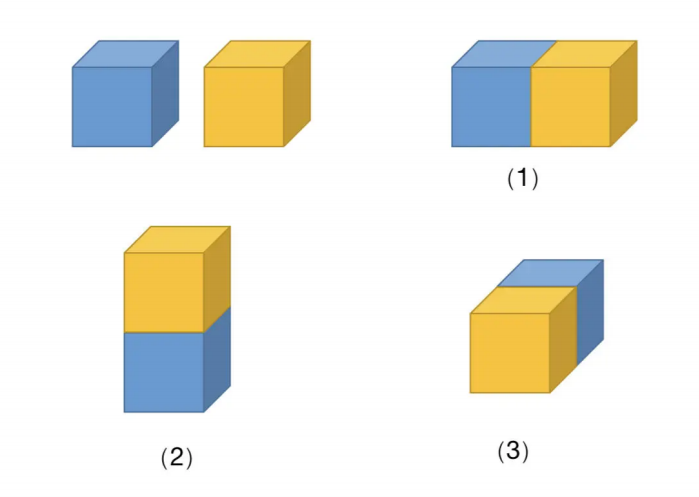
\includegraphics[scale=.3]{part/人工智能/深度学习框架/pic/Pytorch/Pytorch基础/cat的拼接方式.png}
\caption{cat的拼接方式}
\end{minipage}
\hspace{0.05\textwidth} % 调整这里的参数来改变图片之间的空隙
\begin{minipage}[t]{0.45\textwidth}
\centering
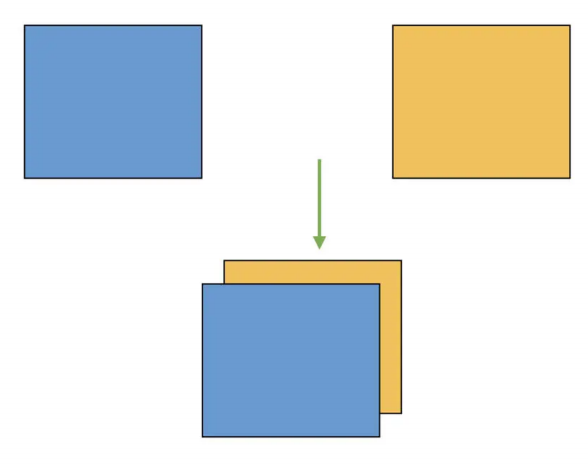
\includegraphics[scale=.3]{part/人工智能/深度学习框架/pic/Pytorch/Pytorch基础/stack的拼接方式.png}
\caption{stack的拼接方式}
\end{minipage}
\caption{cat和stack的拼接方式}
\end{figure}


\codeinline{cat} 实际上是将多个 Tensor 在已有的维度上进行连接，

\subsubsection{stack() 增加维度连接}
\label{subsubsec:Pytorch的stack()函数}
那如果想增加新的维度进行连接，这时候就需要 \codeinline{stack} 函数登场了。
\begin{lstlisting}[style=demostyle,numbers=none]
# stack() 用于连接张量
torch.stack(tensors, dim=0, out=None)
# tensors: 张量序列
# dim: 沿着哪个维度拼接
# out: 输出张量
\end{lstlisting}
\begin{lstlisting}[style=pythonstyle]
import torch

# 两个二维张量
A=torch.ones(3,3)
B=2*torch.ones(3,3)

print("A.size():",A.size())
print("B.size():",B.size())

print("torch.stack((A,B),0).size():",torch.stack((A,B),0).size())
print("torch.stack((A,B),1).size():",torch.stack((A,B),1).size())
print("torch.stack((A,B),2).size():",torch.stack((A,B),2).size())
\end{lstlisting}

\begin{lstlisting}[style=demostyle,numbers=none]
A.size(): torch.Size([3, 3])
B.size(): torch.Size([3, 3])
torch.stack((A,B),0).size(): torch.Size([2, 3, 3])
torch.stack((A,B),1).size(): torch.Size([3, 2, 3])
torch.stack((A,B),2).size(): torch.Size([3, 3, 2])
\end{lstlisting}

\begin{derivation}{推导stack的拼接方式}
    \begin{enumerate}[label=\arabic*)]
        \item 维度0

        对于A的维度0就是第0个括号开始的
        \begin{lstlisting}[style=demostyle,numbers=none]
            [[1., 1., 1.],
             [1., 1., 1.],
             [1., 1., 1.]]
        \end{lstlisting}   
            
        同理B的维度0就是第0个括号开始的
        \begin{lstlisting}[style=demostyle,numbers=none]
            [[2., 2., 2.],
             [2., 2., 2.],
             [2., 2., 2.]]
        \end{lstlisting}

        在维度0上拼接就是将A和B在维度0上合并(新增第0个[]括号)
        \begin{lstlisting}[style=demostyle,numbers=none]
        [ # 新增的维度0
            [[1., 1., 1.],
             [1., 1., 1.],
             [1., 1., 1.]],

            [[2., 2., 2.],
             [2., 2., 2.],
             [2., 2., 2.]]
        ]
        \end{lstlisting}

        \item 维度1

        对于A的维度0就是第1个括号开始的
        \begin{lstlisting}[style=demostyle,numbers=none]
        [   # 这层括号不看了
            [1., 1., 1.],
            [1., 1., 1.],
            [1., 1., 1.]
        ]   # 这层括号不看了
        \end{lstlisting}

        同理B的维度0就是第1个括号开始的
        \begin{lstlisting}[style=demostyle,numbers=none]
        [   # 这层括号不看了
            [2., 2., 2.],
            [2., 2., 2.],
            [2., 2., 2.]
        ]   # 这层括号不看了
        \end{lstlisting}

        在维度1上拼接就是将A和B在维度0上合并(新增第1个[]括号)
        \begin{lstlisting}[style=demostyle,numbers=none]
        [
            [ # 新增第1个[]括号
             [1., 1., 1.],
             [2., 2., 2.]
            ],
   
            [
             [1., 1., 1.],
             [2., 2., 2.]
            ],
   
           [
             [1., 1., 1.],
             [2., 2., 2.]
            ]
        ]
        \end{lstlisting}

        \item 维度2

        对于A的维度0就是第2个括号开始的
        \begin{lstlisting}[style=demostyle,numbers=none]
        [   # 这层括号不看了
            [# 这层括号不看了
                1.,
                1., 
                1.
            ],

            [# 这层括号不看了
                1., 
                1., 
                1.
            ],

            [# 这层括号不看了
                1., 
                1., 
                1.
            ]
        ]   # 这层括号不看了
    \end{lstlisting}

    同理B的维度0就是第2个括号开始的
    \begin{lstlisting}[style=demostyle,numbers=none]
    [   # 这层括号不看了
        [# 这层括号不看了
            2.,
            2., 
            2.
        ],

        [# 这层括号不看了
            2., 
            2., 
            2.
        ],

        [# 这层括号不看了
            2., 
            2., 
            2.
        ]
    ]   # 这层括号不看了
    \end{lstlisting}

    在维度2上拼接就是将A和B在维度0上合并(新增第2个[]括号)
    \begin{lstlisting}[style=demostyle,numbers=none]
    [
        [ 
            [1., 2.], # 新增第2个[]括号
            [1., 2.],
            [1., 2.]
        ],

        [
            [1., 2.],
            [1., 2.],
            [1., 2.]
        ],

        [
            [1., 2.],
            [1., 2.],
            [1., 2.]
        ]
    ]
    \end{lstlisting}

    \end{enumerate}
    
\end{derivation}

详细展开发现

\begin{lstlisting}[style=demostyle,numbers=none]
>>> A=torch.ones(3,3)
>>> B=2*torch.ones(3,3)
>>> A
tensor([[1., 1., 1.],
        [1., 1., 1.],
        [1., 1., 1.]])
>>> B
tensor([[2., 2., 2.],
        [2., 2., 2.],
        [2., 2., 2.]])
>>> torch.stack((A,B),0)
tensor([[[1., 1., 1.],
         [1., 1., 1.],
         [1., 1., 1.]],

        [[2., 2., 2.],
         [2., 2., 2.],
         [2., 2., 2.]]])
>>> torch.stack((A,B),1)
tensor([[[1., 1., 1.],
         [2., 2., 2.]],

        [[1., 1., 1.],
         [2., 2., 2.]],

        [[1., 1., 1.],
         [2., 2., 2.]]])
>>> torch.stack((A,B),2)
tensor([[[1., 2.],
         [1., 2.],
         [1., 2.]],

        [[1., 2.],
         [1., 2.],
         [1., 2.]],

        [[1., 2.],
         [1., 2.],
         [1., 2.]]])
\end{lstlisting}      



\begin{lstlisting}[style=demostyle,numbers=none]
>>> A=torch.arange(0,4)
tensor([0, 1, 2, 3])
>>> B=torch.arange(5,9)
>>> B
tensor([5, 6, 7, 8])

>>> C=torch.stack((A,B),0)
>>> C
tensor([[0, 1, 2, 3],
        [5, 6, 7, 8]])
>>> D=torch.stack((A,B),1)
>>> D
tensor([[0, 5],
        [1, 6],
        [2, 7],
        [3, 8]])
\end{lstlisting}

\subsection{Tensor的切片}
\label{subsec:Pytorch的Tensor的切片}
切分就是连接的逆过程，有了刚才的经验

PyTorch 中的 Tensor 支持切片操作，但是切片操作会返回一个新的 Tensor，
所以切片操作不会改变原来的 Tensor。

PyTorch提供了\codeinline{chunk()}、\codeinline{split()}和\codeinline{unbind()}函数来实现切片操作。

\subsubsection{chunk() 均分}
\label{subsubsec:Pytorch的chunk()函数}
\begin{lstlisting}[style=demostyle,numbers=none]
# chunk() 按照声明的 dim，进行尽可能平均的划分。
# 如果不能整除，则最后一个张量的维度会小于其他张量

torch.chunk(tensor, chunks, dim=0)
# tensor: 输入张量
# chunks: 切分后的块数
# dim: 切分维度
\end{lstlisting}
\begin{lstlisting}[style=pythonstyle]
import torch

# 示例1：一维张量的均分
A = torch.tensor([1, 2, 3, 4, 5, 6, 7, 8, 9, 10])

# 将A沿着dim=0方向均分为2个块
B = torch.chunk(A, 2, 0)
print("示例1：一维张量的均分")
for i, chunk in enumerate(B):
    print(f"块{i+1}:", chunk)

# 示例2：一维张量不能均分的情况
# 将A沿着dim=0方向分成3个块，不能整除的情况下最后一个块包含剩余元素
C = torch.chunk(A, 3, 0)
print("\n示例2：一维张量不能均分的情况")
for i, chunk in enumerate(C):
    print(f"块{i+1}:", chunk)

# 示例3：二维张量的分块
D = torch.tensor([[1, 2, 3], [4, 5, 6], [7, 8, 9], [10, 11, 12]])

# 将D沿着dim=0（行方向）分成2个块
E = torch.chunk(D, 2, 0)
print("\n示例3：二维张量沿行方向的均分")
for i, chunk in enumerate(E):
    print(f"块{i+1}:\n", chunk)

# 将D沿着dim=1（列方向）分成2个块
# chunk 函数是先做除法，然后再向上取整得到每组的数量。
F = torch.chunk(D, 2, 1)
print("\n示例4：二维张量沿列方向的均分")
for i, chunk in enumerate(F):
    print(f"块{i+1}:\n", chunk)

# 示例5：如果 chunk 参数大于 Tensor 可以切分的长度
# 将D沿着dim=1（列方向）分成4个块，不均分时，最后一个块包含剩余的元素
G = torch.chunk(D, 4, 1)
print("\n示例5：二维张量沿列方向不能均分的情况")
for i, chunk in enumerate(G):
    print(f"块{i+1}:\n", chunk)

# 示例6：三维张量的分块
H = torch.tensor([[[1, 2], [3, 4]], [[5, 6], [7, 8]], [[9, 10], [11, 12]]])

# 将H沿着dim=0（最外层维度）分成3个块
I = torch.chunk(H, 3, 0)
print("\n示例6：三维张量沿最外层维度的均分")
for i, chunk in enumerate(I):
    print(f"块{i+1}:\n", chunk)
\end{lstlisting}
\begin{lstlisting}[style=demostyle,numbers=none]
示例1：一维张量的均分
块1: tensor([1, 2, 3, 4, 5])
块2: tensor([ 6,  7,  8,  9, 10])

示例2：一维张量不能均分的情况
块1: tensor([1, 2, 3, 4])
块2: tensor([5, 6, 7, 8])
块3: tensor([ 9, 10])

示例3：二维张量沿行方向的均分
块1:
tensor([[1, 2, 3],
        [4, 5, 6]])
块2:
tensor([[ 7,  8,  9],
        [10, 11, 12]])

示例4：二维张量沿列方向的均分
块1:
tensor([[ 1,  2],
        [ 4,  5],
        [ 7,  8],
        [10, 11]])
块2:
tensor([[ 3],
        [ 6],
        [ 9],
        [12]])

示例5：如果 chunk 参数大于 Tensor 可以切分的长度
块1:
tensor([[ 1],
        [ 4],
        [ 7],
        [10]])
块2:
tensor([[ 2],
        [ 5],
        [ 8],
        [11]])
块3:
tensor([[ 3],
        [ 6],
        [ 9],
        [12]])

示例6：三维张量沿最外层维度的均分
块1:
tensor([[[1, 2],
        [3, 4]]])
块2:
tensor([[[5, 6],
        [7, 8]]])
块3:
tensor([[[ 9, 10],
        [11, 12]]])
\end{lstlisting}

\subsubsection{split() 按照指定大小切分}
\label{subsubsec:Pytorch的split()函数}
\begin{lstlisting}[style=demostyle,numbers=none]
# split() 按照声明的 dim，进行划分。
torch.split(tensor, split_size_or_sections, dim=0)
# split_size_or_sections 这个参数。
#   当它为整数时，表示将 tensor 按照每块大小为这个整数的数值来切割；
#   当这个参数为列表时，则表示将此 tensor 切成和列表中元素一样大小的块。
# 
#   如果使用list,要保证 list的和等于 改维度的大小
\end{lstlisting}
\begin{lstlisting}[style=pythonstyle]
import torch

# 示例1：一维张量，按照固定大小分割l
A = torch.tensor([1, 2, 3, 4, 5, 6, 7, 8, 9, 10])

# 将A按照每块大小为3进行分割，dim=0（默认）
B = torch.split(A, 3, 0)
print("示例1：一维张量，按照固定大小分割")
for i, chunk in enumerate(B):
    print(f"块{i+1}:", chunk)

# 示例2：一维张量，不能均分的情况
# 将A按照每块大小为4进行分割，最后一个块包含剩余元素
C = torch.split(A, 4, 0)
print("\n示例2：一维张量，不能均分的情况")
for i, chunk in enumerate(C):
    print(f"块{i+1}:", chunk)

# 示例3：一维张量，按照列表分割
# 将A按照列表[2, 3, 5]指定的块大小进行分割
# 
# 这里第0维度一共10个元素，因此 list 中的元素之和应该等于 10=2+3+5
D = torch.split(A, [2, 3, 5], 0)
print("\n示例3：一维张量，按照列表分割")
for i, chunk in enumerate(D):
    print(f"块{i+1}:", chunk)

# 示例4：二维张量，按行分割
E = torch.tensor([[1, 2, 3], [4, 5, 6], [7, 8, 9], [10, 11, 12]])

# 将E沿着dim=0（行方向）按照每块大小为2进行分割
F = torch.split(E, 2, 0)
print("\n示例4：二维张量，按行分割")
for i, chunk in enumerate(F):
    print(f"块{i+1}:\n", chunk)

# 示例5：二维张量，按列分割
# 将E沿着dim=1（列方向）按照每块大小为2进行分割
G = torch.split(E, 2, 1)
print("\n示例5：二维张量，按列分割")
for i, chunk in enumerate(G):
    print(f"块{i+1}:\n", chunk)

# 示例6：二维张量，不能均分的情况
# 将E沿着dim=1（列方向）分成[1, 2]两块
H = torch.split(E, [1, 2], 1)
print("\n示例6：二维张量，不能均分的情况")
for i, chunk in enumerate(H):
    print(f"块{i+1}:\n", chunk)

# 示例7：三维张量，按最外层维度分割
I = torch.tensor([[[1, 2], [3, 4]], [[5, 6], [7, 8]], [[9, 10], [11, 12]]])

# 将I沿着dim=0分割成每块大小为1的块
J = torch.split(I, 1, 0)
print("\n示例7：三维张量，按最外层维度分割")
for i, chunk in enumerate(J):
    print(f"块{i+1}:\n", chunk)

# 示例8：三维张量，按第二维度分割
# 将I沿着dim=1（第二维度）分割成每块大小为1的块
K = torch.split(I, 1, 1)
print("\n示例8：三维张量，按第二维度分割")
for i, chunk in enumerate(K):
    print(f"块{i+1}:\n", chunk)
\end{lstlisting}
\begin{lstlisting}[style=demostyle,numbers=none]
示例1：一维张量，按照固定大小分割
块1: tensor([1, 2, 3])
块2: tensor([4, 5, 6])
块3: tensor([7, 8, 9])
块4: tensor([10])

示例2：一维张量，不能均分的情况
块1: tensor([1, 2, 3, 4])
块2: tensor([5, 6, 7, 8])
块3: tensor([ 9, 10])

示例3：一维张量，按照列表分割
块1: tensor([1, 2])
块2: tensor([3, 4, 5])
块3: tensor([ 6,  7,  8,  9, 10])

示例4：二维张量，按行分割
块1:
tensor([[1, 2, 3],
        [4, 5, 6]])
块2:
tensor([[ 7,  8,  9],
        [10, 11, 12]])

示例5：二维张量，按列分割
块1:
tensor([[ 1,  2],
        [ 4,  5],
        [ 7,  8],
        [10, 11]])
块2:
tensor([[ 3],
        [ 6],
        [ 9],
        [12]])

示例6：二维张量，不能均分的情况
块1:
tensor([[ 1],
        [ 4],
        [ 7],
        [10]])
块2:
tensor([[ 2,  3],
        [ 5,  6],
        [ 8,  9],
        [11, 12]])

示例7：三维张量，按最外层维度分割
块1:
tensor([[[1, 2],
        [3, 4]]])
块2:
tensor([[[5, 6],
        [7, 8]]])
块3:
tensor([[[ 9, 10],
        [11, 12]]])

示例8：三维张量，按第二维度分割
块1:
tensor([[[ 1,  2]],

        [[ 5,  6]],

        [[ 9, 10]]])
块2:
tensor([[[ 3,  4]],

        [[ 7,  8]],

        [[11, 12]]])
\end{lstlisting}

\subsubsection{unbind() 按照指定维度切分}
\label{subsubsec:Pytorch的unbind()}
如果我们现在有一个 3 channel 图像的 Tensor，想要逐个获取每个 channel 的数据,
假如用 \codeinline{chunk} 的话，我们需要将 \codeinline{chunks} 设为 3；
如果用 \codeinline{split} 的话，需要将 \codeinline{split\_size\_or\_sections} 设为 1.

虽然它们都可以实现相同的目的，但是如果 channel 数量很大，逐个去取也比较折腾。
这时候，就需要用到另一个函数：\codeinline{unbind}，它的函数定义如下
\begin{lstlisting}[style=demostyle,numbers=none]
# unbind() 按照声明的 dim，进行切分。
torch.unbind(tensor, dim=0)
\end{lstlisting}

\begin{lstlisting}[style=pythonstyle]
import torch

# 示例1：三通道图像的三维张量，按第一个维度分割
# 假设我们有一个三通道的图像张量，大小为 (3, 4, 4)
image_tensor = torch.tensor([
    [[1, 2, 3, 4], [5, 6, 7, 8], [9, 10, 11, 12], [13, 14, 15, 16]],    # 第一个通道
    [[17, 18, 19, 20], [21, 22, 23, 24], [25, 26, 27, 28], [29, 30, 31, 32]], # 第二个通道
    [[33, 34, 35, 36], [37, 38, 39, 40], [41, 42, 43, 44], [45, 46, 47, 48]]  # 第三个通道
])

# 使用unbind方法按dim=0分割（将每个通道分开）
channels = torch.unbind(image_tensor, dim=0)
print("示例1：三通道图像张量按dim=0分割")
for i, channel in enumerate(channels):
    print(f"通道{i+1}:\n", channel)

# 示例2：二维张量，按行分割
tensor_2d = torch.tensor([[1, 2, 3], [4, 5, 6], [7, 8, 9]])

# 使用unbind方法按dim=0分割（按行分割）
rows = torch.unbind(tensor_2d, dim=0)
print("\n示例2：二维张量按行分割")
for i, row in enumerate(rows):
    print(f"行{i+1}:", row)

# 使用unbind方法按dim=1分割（按列分割）
cols = torch.unbind(tensor_2d, dim=1)
print("\n示例3：二维张量按列分割")
for i, col in enumerate(cols):
    print(f"列{i+1}:", col)

# 示例4：三维张量，按第二维度分割
tensor_3d = torch.tensor([
    [[1, 2], [3, 4], [5, 6]],
    [[7, 8], [9, 10], [11, 12]]
])

# 使用unbind方法按dim=1分割（按第二维度分割，即分割每个二维张量）
split_second_dim = torch.unbind(tensor_3d, dim=1)
print("\n示例4：三维张量按第二维度分割")
for i, sub_tensor in enumerate(split_second_dim):
    print(f"分块{i+1}:\n", sub_tensor)

# 示例5：四维张量，按第三维度分割
tensor_4d = torch.tensor([
    [[[1], [2]], [[3], [4]]],
    [[[5], [6]], [[7], [8]]]
])

# 使用unbind方法按dim=2分割（按第三维度分割）
split_third_dim = torch.unbind(tensor_4d, dim=2)
print("\n示例5：四维张量按第三维度分割")
for i, sub_tensor in enumerate(split_third_dim):
    print(f"分块{i+1}:\n", sub_tensor)
\end{lstlisting}
\begin{lstlisting}[style=demostyle,numbers=none]
示例1：三通道图像张量按dim=0分割
通道1:
    tensor([[ 1,  2,  3,  4],
        [ 5,  6,  7,  8],
        [ 9, 10, 11, 12],
        [13, 14, 15, 16]])
通道2:
    tensor([[17, 18, 19, 20],
        [21, 22, 23, 24],
        [25, 26, 27, 28],
        [29, 30, 31, 32]])
通道3:
    tensor([[33, 34, 35, 36],
        [37, 38, 39, 40],
        [41, 42, 43, 44],
        [45, 46, 47, 48]])

示例2：二维张量按行分割
行1: tensor([1, 2, 3])
行2: tensor([4, 5, 6])
行3: tensor([7, 8, 9])

示例3：二维张量按列分割
列1: tensor([1, 4, 7])
列2: tensor([2, 5, 8])
列3: tensor([3, 6, 9])

示例4：三维张量按第二维度分割
分块1:
    tensor([[1, 2],
        [7, 8]])
分块2:
    tensor([[ 3,  4],
        [ 9, 10]])
分块3:
    tensor([[ 5,  6],
        [11, 12]])

示例5：四维张量按第三维度分割
分块1:
    tensor([[[1],
            [3]],

        [[5],
            [7]]])
分块2:
    tensor([[[2],
            [4]],

        [[6],
            [8]]])
\end{lstlisting}

\subsection{根据操作张量中的元素分类}
\label{subsec:Pytorch的根据操作张量中的元素分类}
\subsubsection{逐元素操作}
\label{subsec:Pytorch逐元素操作}
如表 \ref{tab:Pytorch逐元素操作} 所示，PyTorch 提供了很多逐元素操作的函数，可以对张量进行逐元素操作。
\begin{table}[h]
\centering
\begin{tabular}{|l|l|}
\hline
\textbf{函数} & \textbf{说明} \\ \hline
\codeinline{abs/add} & 绝对值 / 加法 \\ \hline
\codeinline{addcdiv(t, t1, t2, value=1)} & \codeinline{t1} 与 \codeinline{t2} 按元素除后，乘以 \codeinline{value} 加 \codeinline{t} \\ \hline
\codeinline{addcmul(t, t1, t2, value=1)} & \codeinline{t1} 与 \codeinline{t2} 按元素乘后，乘以 \codeinline{value} 加 \codeinline{t} \\ \hline
\codeinline{ceil/floor} & 向上取整 / 向下取整 \\ \hline
\codeinline{clamp(t, min, max)} & 将张量元素限制在指定区间 \\ \hline
\codeinline{exp/log/pow} & 指数 / 对数 / 幂 \\ \hline
\codeinline{mul(*tensor) / neg} & 逐元素乘法 / 取反 \\ \hline
\codeinline{sigmoid/tanh/softmax} & 激活函数 \\ \hline
\codeinline{sign/sqrt} & 取符号 / 开根号 \\ \hline
\end{tabular}
\caption{常见的逐元素操作}
\label{tab:Pytorch逐元素操作}
\end{table}
\begin{lstlisting}[style=pythonstyle]
import torch

# Initial tensor for demonstration
t = torch.tensor([[1.0, -2.0], [3.0, -4.0]])
t1 = torch.tensor([[2.0, 2.0], [2.0, 2.0]])
t2 = torch.tensor([[1.0, -1.0], [-1.0, 1.0]])

print("Initial Tensor t:\n", t)
print("Tensor t1:\n", t1)
print("Tensor t2:\n", t2)

# 1. abs/add
abs_result = torch.abs(t)
add_result = torch.add(t, t1)
print("\nabs(t):\n", abs_result)
print("add(t, t1):\n", add_result)

# 2. addcdiv(t, t1, t2, value=1)
addcdiv_result = torch.addcdiv(t, t1, t2, value=1)
print("\naddcdiv(t, t1, t2, value=1):\n", addcdiv_result)

# 3. addcmul(t, t1, t2, value=1)
addcmul_result = torch.addcmul(t, t1, t2, value=1)
print("\naddcmul(t, t1, t2, value=1):\n", addcmul_result)

# 4. ceil/floor
ceil_result = torch.ceil(t)
floor_result = torch.floor(t)
print("\nceil(t):\n", ceil_result)
print("floor(t):\n", floor_result)

# 5. clamp(t, min, max)
clamp_result = torch.clamp(t, min=-1, max=1)
print("\nclamp(t, min=-1, max=1):\n", clamp_result)

# 6. exp/log/pow
exp_result = torch.exp(t)
log_result = torch.log(torch.abs(t) + 1)  # Add 1 to avoid log(0)
pow_result = torch.pow(t, 2)
print("\nexp(t):\n", exp_result)
print("log(abs(t) + 1):\n", log_result)
print("pow(t, 2):\n", pow_result)

# 7. mul(*tensor)/neg
mul_result = torch.mul(t, t1)
neg_result = torch.neg(t)
print("\nmul(t, t1):\n", mul_result)
print("neg(t):\n", neg_result)

# 8. sigmoid/tanh/softmax
sigmoid_result = torch.sigmoid(t)
tanh_result = torch.tanh(t)
softmax_result = torch.softmax(t, dim=0)
print("\nsigmoid(t):\n", sigmoid_result)
print("tanh(t):\n", tanh_result)
print("softmax(t, dim=0):\n", softmax_result)

# 9. sign/sqrt
sign_result = torch.sign(t)
sqrt_result = torch.sqrt(torch.abs(t))  # sqrt on abs to avoid sqrt of negative
print("\nsign(t):\n", sign_result)
print("sqrt(abs(t)):\n", sqrt_result)
\end{lstlisting}
\begin{lstlisting}[style=demostyle,numbers=none]
Initial Tensor t:
 tensor([[ 1., -2.],
        [ 3., -4.]])
Tensor t1:
 tensor([[2., 2.],
        [2., 2.]])
Tensor t2:
 tensor([[ 1., -1.],
        [-1.,  1.]])

abs(t):
 tensor([[1., 2.],
        [3., 4.]])
add(t, t1):
 tensor([[ 3.,  0.],
        [ 5., -2.]])

addcdiv(t, t1, t2, value=1):
 tensor([[ 3., -4.],
        [ 1., -2.]])

addcmul(t, t1, t2, value=1):
 tensor([[ 3., -4.],
        [ 1., -2.]])

ceil(t):
 tensor([[ 1., -2.],
        [ 3., -4.]])
floor(t):
 tensor([[ 1., -2.],
        [ 3., -4.]])

clamp(t, min=-1, max=1):
 tensor([[ 1., -1.],
        [ 1., -1.]])

exp(t):
 tensor([[2.7183e+00, 1.3534e-01],
        [2.0086e+01, 1.8316e-02]])
log(abs(t) + 1):
 tensor([[0.6931, 1.0986],
        [1.3863, 1.6094]])
pow(t, 2):
 tensor([[ 1.,  4.],
        [ 9., 16.]])

mul(t, t1):
 tensor([[ 2., -4.],
        [ 6., -8.]])
neg(t):
 tensor([[-1.,  2.],
        [-3.,  4.]])

sigmoid(t):
 tensor([[0.7311, 0.1192],
        [0.9526, 0.0180]])
tanh(t):
 tensor([[ 0.7616, -0.9640],
        [ 0.9951, -0.9993]])
softmax(t, dim=0):
 tensor([[0.1192, 0.8808],
        [0.8808, 0.1192]])

sign(t):
 tensor([[ 1., -1.],
        [ 1., -1.]])
sqrt(abs(t)):
 tensor([[1.0000, 1.4142],
        [1.7321, 2.0000]])
\end{lstlisting}
\subsubsection{in-place操作}
\label{subsec:Pytorch的in-place操作}
在 PyTorch 中，in-place 操作是指那些直接在原地修改张量内容的操作，
而不是创建新的张量。
in-place 操作通常以 \codeinline{\_} 结尾。

\begin{enumerate}[label=\arabic*)]
        \item 数学运算
        \begin{enumerate}[itemindent=1em,label=\arabic*)]
                \item \codeinline{add\_()}: 加法操作
                \item \codeinline{sub\_()}: 减法操作
                \item \codeinline{mul\_()}: 乘法操作
                \item \codeinline{div\_()}: 除法操作
                \item \codeinline{pow\_()}: 幂操作
        \end{enumerate}
    
        \item 张量变形和索引操作
        \begin{enumerate}[itemindent=1em,label=\arabic*)]
                \item \codeinline{view\_()}: 变形操作
                \item \codeinline{reshape\_()}: 变形操作
                \item \codeinline{resize\_()}: 调整张量大小
                \item \codeinline{zero\_()}: 将张量的所有元素置为 0
                \item \codeinline{fill\_()}: 用指定的值填充张量
        \end{enumerate}
    
        \item 其他操作
        \begin{enumerate}[itemindent=1em,label=\arabic*)]
                \item \codeinline{copy\_()}: 将一个张量的内容复制到另一个张量
                \item \codeinline{index\_add\_()}: 按指定的索引对张量进行加法操作
                \item \codeinline{index\_copy\_()}: 按指定的索引对张量进行复制操作
                \item \codeinline{index\_fill\_()}: 按指定的索引对张量进行填充操作
        \end{enumerate}
    
        \item 归一化操作
        \codeinline{normalize\_()}：对张量进行归一化操作
\end{enumerate}


\begin{lstlisting}[style=pythonstyle]
import torch

# 创建一个张量
x = torch.tensor([1.0, 2.0, 3.0], requires_grad=True)

# In-place 操作示例
x.add_(1.0)       # x = [2.0, 3.0, 4.0]
x.mul_(2.0)       # x = [4.0, 6.0, 8.0]
x.zero_()        # x = [0.0, 0.0, 0.0]

# 需要注意，进行 in-place 操作时，可能会导致计算图被破坏
y = x.sum()
y.backward()     # 如果x是叶子节点，可能会报错
\end{lstlisting}

\subsubsection{内存布局连续}
\label{subsec:Pytorch的内存布局连续}
\begin{enumerate}[label=\arabic*)]
    \item 连续的 Tensor（Contiguous Tensor）：如果张量的元素在内存中是按行优先（row-major order）连续存储的，则称该张量是连续的。换句话说，张量的内存布局按照其自身的存储顺序（从前到后）逐行排列，不存在任何跳跃或间隔。

    \item 不连续的 Tensor（Non-contiguous Tensor）：不连续的张量是在内存中不按行优先存储的。这通常发生在张量经过某些操作（如转置、切片等）后，其数据不再按顺序排列，而是产生了间隔或跳跃。在这种情况下，张量的数据虽然依然可以访问，但可能需要额外的内存和计算来访问这些非连续存储的数据。
\end{enumerate}

PyTorch 提供了 \codeinline{is\_contiguous()} 方法来检查张量是否是连续的，如果张量是连续的，则返回 \codeinline{True}，否则返回 \codeinline{False}。
\begin{lstlisting}[style=pythonstyle]
import torch

# 创建一个张量
x = torch.tensor([[1.0, 2.0, 3.0], [4, 5, 6]], requires_grad=True)

# 检查张量是否是连续的
is_contiguous = x.is_contiguous()
print("x 是否是连续的: ", x.is_contiguous())

# 创建一个不连续的张量
y = x.t()
print("y 是否是连续的: ", y.is_contiguous())
\end{lstlisting}
\begin{lstlisting}[style=demostyle,numbers=none]
x 是否是连续的:  True
y 是否是连续的:  False
\end{lstlisting}

导致张量不连续的原因一下的操作：
\begin{enumerate}[label=\arabic*)]
    \item 转置操作（Transpose）：

    转置操作 \codeinline{x.t()} 或 \codeinline{x.transpose(dim0, dim1)} 
    会导致张量的存储顺序改变。
    因为转置操作会交换维度，使得在内存中的数据顺序不再是行优先的。

    \item 切片（Slicing）：
    
    对张量的部分切片操作，例如 \codeinline{x[:, ::2]}，
    也可能导致不连续。因为切片操作可能会跳过一部分数据，导致数据在内存中不再按顺序排列。
    
    \item 视图操作（View）：
    
    某些视图操作，如 \codeinline{x.view(-1, 2)}，可能需要重新排列内存中的数据。如果操作需要重新安排数据，结果张量可能是非连续的。
    
    \item 拼接（Concatenation）：
    
    例如 \codeinline{torch.cat([x1, x2], dim=0)} 如果在非连续维度上拼接，也可能产生不连续的结果。
    
    \item 高维交换（Permute）：
    
    \codeinline{x.permute(dims)} 操作会重新排列张量的维度，使其不再连续。
\end{enumerate}
\begin{lstlisting}[style=pythonstyle]
import torch

# 创建一个张量
x = torch.tensor([[1.0, 2.0, 3.0], [4, 5, 6]], requires_grad=True)

# 检查张量是否是连续的
print("x 是否是连续的: ", x.is_contiguous())

# 转置操作（Transpose）
y = x.t()
print("转置后的 y 是否是连续的: ", y.is_contiguous())  # 转置操作导致不连续

# 切片操作（Slicing）
z = x[:, ::2]  # 每隔一个元素切片
print("切片后的 z 是否是连续的: ", z.is_contiguous())  # 切片操作导致不连续

# 视图操作（View）
v = x.view(-1)  # 将张量展平为一维
print("视图后的 v 是否是连续的: ", v.is_contiguous())  # 视图操作不改变内存顺序，仍然是连续的

# 拼接操作（Concatenation）
a = torch.tensor([[7.0, 8.0, 9.0], [10, 11, 12]], requires_grad=True)
w = torch.cat([x, a], dim=0)  # 沿第0维进行拼接
print("拼接后的 w 是否是连续的: ", w.is_contiguous())  # 沿着同一个维度拼接，结果是连续的

# 高维交换（Permute）
p = x.permute(1, 0)  # 交换维度
print("高维交换后的 p 是否是连续的: ", p.is_contiguous())  # 高维交换操作导致不连续

# 结果分析
# 1. 转置操作（Transpose）会导致张量不连续，因为转置改变了元素在内存中的排列顺序。
# 2. 切片操作（Slicing）可能导致不连续，特别是切片间隔（如 [::2]）操作会跳过一些数据，破坏了连续性。
# 3. 视图操作（View）在张量连续的前提下，不改变内存顺序，因此结果仍然是连续的。
# 4. 沿着同一个维度进行拼接（Concatenation）一般不会改变张量的连续性，拼接后的张量是连续的。
# 5. 高维交换（Permute）操作改变了维度顺序，从而导致不连续。

# 对比总结
# - 转置（Transpose）、切片（Slicing，尤其是步长不为1的切片）和高维交换（Permute）操作通常会导致张量变为不连续。
# - 视图操作（View）和沿着同一维度的拼接（Concatenation）不会影响连续性，只要它们不需要重新排列数据。
\end{lstlisting}
\begin{lstlisting}[style=demostyle,numbers=none]
x 是否是连续的:  True
转置后的 y 是否是连续的:  False
切片后的 z 是否是连续的:  False
视图后的 v 是否是连续的:  True
拼接后的 w 是否是连续的:  True
高维交换后的 p 是否是连续的:  False
\end{lstlisting}




\section{autograd自动求导微分}
\label{sec:Pytorch的autograd自动求导微分}
\subsection{Tensor与Variable}
\label{subsubsec:Pytorch的Tensor与Variable}
\reminder{\lefthand}{在PyTorch 0.4.0版本之后，\codeinline{Variable}已经被弃用，
\textcolor{red}{Tensor}已经整合了Variable的功能。}
虽然Variable仍可用，但Variable返回值已经是一个Tensor（原来返回值是Variable），所以今后无需再用Variable包装Tensor。
但是了解Variable的概念有助于理解PyTorch的自动求导机制。

Variable不仅能对Tensor包装，而且能记录生成Tensor的运算（这是自动求导的关键）。
\begin{lstlisting}[style=demostyle,numbers=none]
torch.autograd.Variable{
    data,           # 就是 Tensor 张量数据
    # 下面的是Tensor梯度运算的记录
    requires_grad,  # 是否需要梯度,
                    # 并不是所有的张量都需要求导，为了节省内存
                    # 只有需要求导的张量才会计算梯度
    grad,           # 对应于data的梯度，形状与data一致
    grad_fn,        # 记录创建该Tensor时用到的Function,
                    # 该Function在反向传播计算中使用
                    # 是自动求导的关键
    is_leaf         # 是否是叶子节点
                    # 为叶子结点时，反向传播结束，其梯度仍会保存，
                    # 非叶子结点的梯度被释放，以节省内存。
}
\end{lstlisting}

0.4.0版本以后，Variable并入Tensor，
可见第\pageref{subsec:Pytorch-Tensor的结构属性}页的Tensor属性。

\begin{lstlisting}[style=demostyle,numbers=none]
torch.Tensor{
    # 与数据相关
    data,           # 张量数据，多维数组，最核心的属性
    dtype,          # 张量类型
    shape,          # 张量形状
    device,         # 张量在CPU或GPU上
    # 与梯度相关
    requires_grad,  # 是否需要梯度,
                    # 并不是所有的张量都需要求导，为了节省内存
                    # 只有需要求导的张量才会计算梯度
    grad,           # 梯度
    grad_fn,        # 创建Tensor的Function,是自动求导的关键
    is_leaf         # 是否是叶子节点
}
\end{lstlisting}
神经网络中的一个重要内容就是参数学习，而参数学习离不开求导。

几乎所有机器学习算法在训练或预测时都归结为求解最优化问题，如果目标函数可导， 
那么问题变为训练函数的驻点（即一阶导数等于零的点）。自动微分也称自动求导，
算法能够计算可导函数在某点处的导数值，是反向传播算法的一般化。

\codeinline{torch.autograd}包就是用来\textcolor{YBXPurple}{自动求导的}。
autograd包为张量上所有的操作提供了自动求导功能，\codeinline{torch.Tensor}和
\codeinline{torch.Function}为autograd包的两个核心类，
它们相互连接并生成一个有向非循环图。

\subsection{自动求导要点}
\label{subsec:Pytorch的自动求导要点}
\codeinline{autograd}包为对Tensor进行自动求导，自动求导时需考虑如下事项：
\begin{enumerate}[label=\arabic*)]
    \item 创建叶子节点（leaf node）：
    通过设置 \codeinline{requires\_grad=True}，可以记录对张量的操作，以便后续利用\codeinline{backward()}进行梯度计算。

    默认情况下，\codeinline{requires\_grad} 为 False。

    \item 修改 \codeinline{requires\_grad}：
    可以通过 \codeinline{.detach()} 或使用 \codeinline{torch.no\_grad()} 方法来临时禁止梯度计算，不记录计算历史。
    这种方式通常在评估或测试模型时使用。

    历史记录包含了如何创建张量，以及对张量的操作，这些信息被保存在 \codeinline{grad\_fn} 属性中。
    
    \item 非叶子节点的梯度计算：
    通过非叶子节点计算的张量会自动赋予 \codeinline{grad\_fn} 属性，这表明该张量是通过某个操作计算得到的。
    
    \item 调用 \codeinline{backward()}：
    当对最终得到的张量调用 \codeinline{backward()} 方法时，会计算其梯度，
    并且会将梯度累加到叶子节点的 grad 属性中。
    
    \item 指定 backward() 的梯度参数：
    可以指定 \codeinline{backward()} 中的 gradient 参数，其形状应该与调用 \codeinline{backward()} 的张量维度匹配或是可广播的。
    
    \item 反向传播的计算图：
    默认情况下，计算图在反向传播后会被释放，如果需要多次进行反向传播，
    则需要在调用 \codeinline{backward()} 时将 \codeinline{retain\_graph=True}。
    
    \item 非叶子节点的梯度：
    非叶子节点的梯度在调用 \codeinline{backward()} 时会被清除。
    
    \item 禁止自动求导：
    通过 \codeinline{torch.no\_grad()} 可以暂时禁止自动求导，例如在测试或评估模型时。
\end{enumerate}

在整个过程中，PyTorch采用计算图的形式进行组织，该计算图为动态图，
它的计算图在每次前向传播时都会重新构建，这样可以避免计算图过大导致的内存占用问题。

\subsection{计算图}
\label{subsec:Pytorch的计算图}
计算图是一种有向无环图，用来表示算子与变量之间关系的\textcolor{YBXPurple}{有向无环图}。

\subsubsection{计算图的推导}
\label{subsubsec:Pytorch的计算图的推导}
\begin{derivation}{推导计算图过程}
    
    用计算图表示表达式$z = w * x + b$

    如图\ref{fig:前向传播计算图}所示，
    表达式$z = wx+b$可写成两个表示式：如果 $y = wx$,$z=y + b$。

    其中$x, w, b$为变量,是用户创建的变量，不依赖于其他变量，故又称为\textcolor{blue}{\textbf{叶子节点}}。

    为计算各叶子节点的梯度，需要把对应的张量参数\codeinline{requires\_grad}属性设置为\codeinline{True},
    这样就可自动跟踪其历史记录。$y, z$是计算得到的变量，非叶子节点，$z$为根节点。
    \codeinline{mul}和\codeinline{add}是算子（或操作或函数）。
    这些变量及算子就构成一个完整的计算过程（或正向传播过程）。

    \begin{figure}[htbp]
    \centering
    \begin{minipage}[t]{0.4\textwidth}
    \centering
    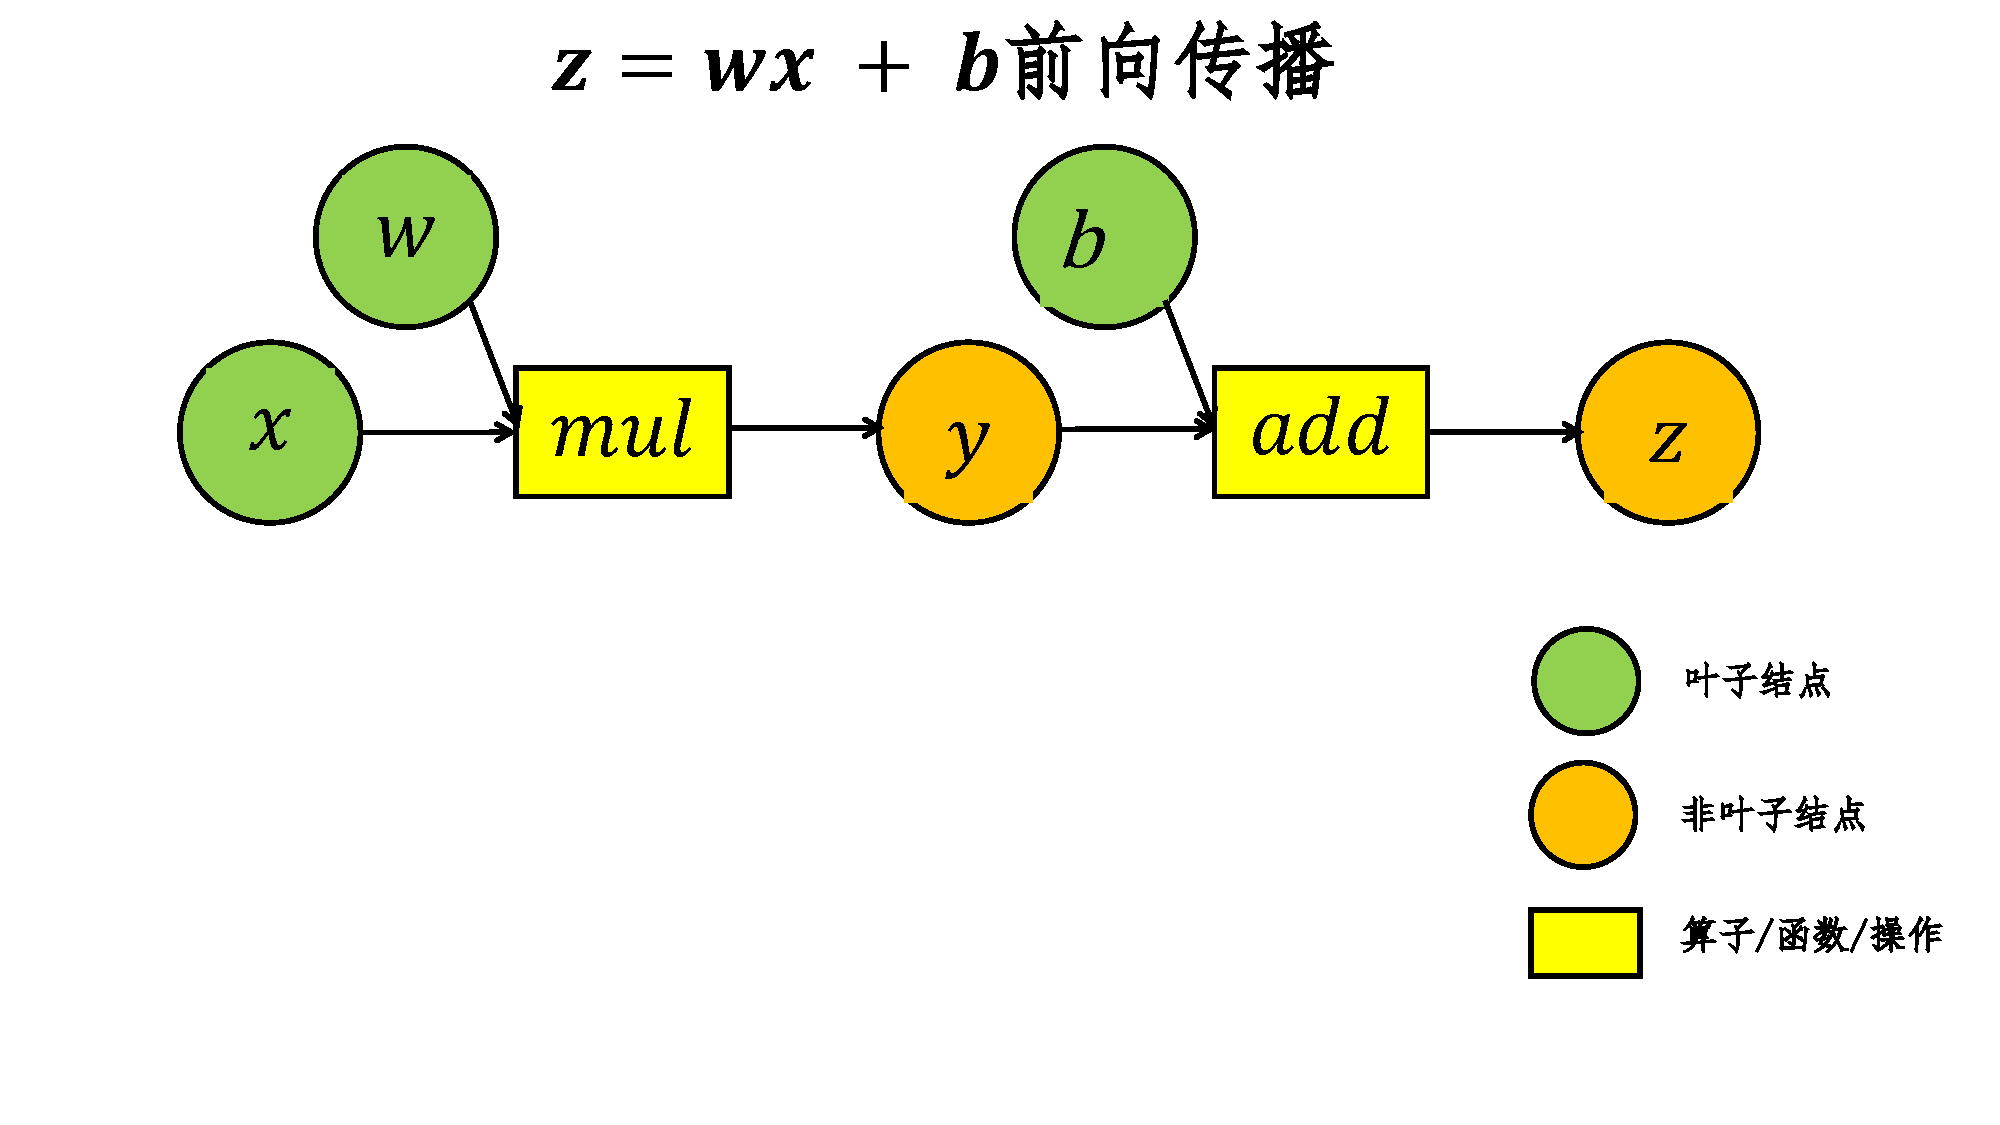
\includegraphics[width=0.5\textwidth]{part/人工智能/深度学习框架/pic/Pytorch/Pytorch基础/前向传播计算图.pdf}
    \caption{\label{fig:前向传播计算图}前向传播计算图}
    \end{minipage}
    \begin{minipage}[t]{0.4\textwidth}
    \centering
    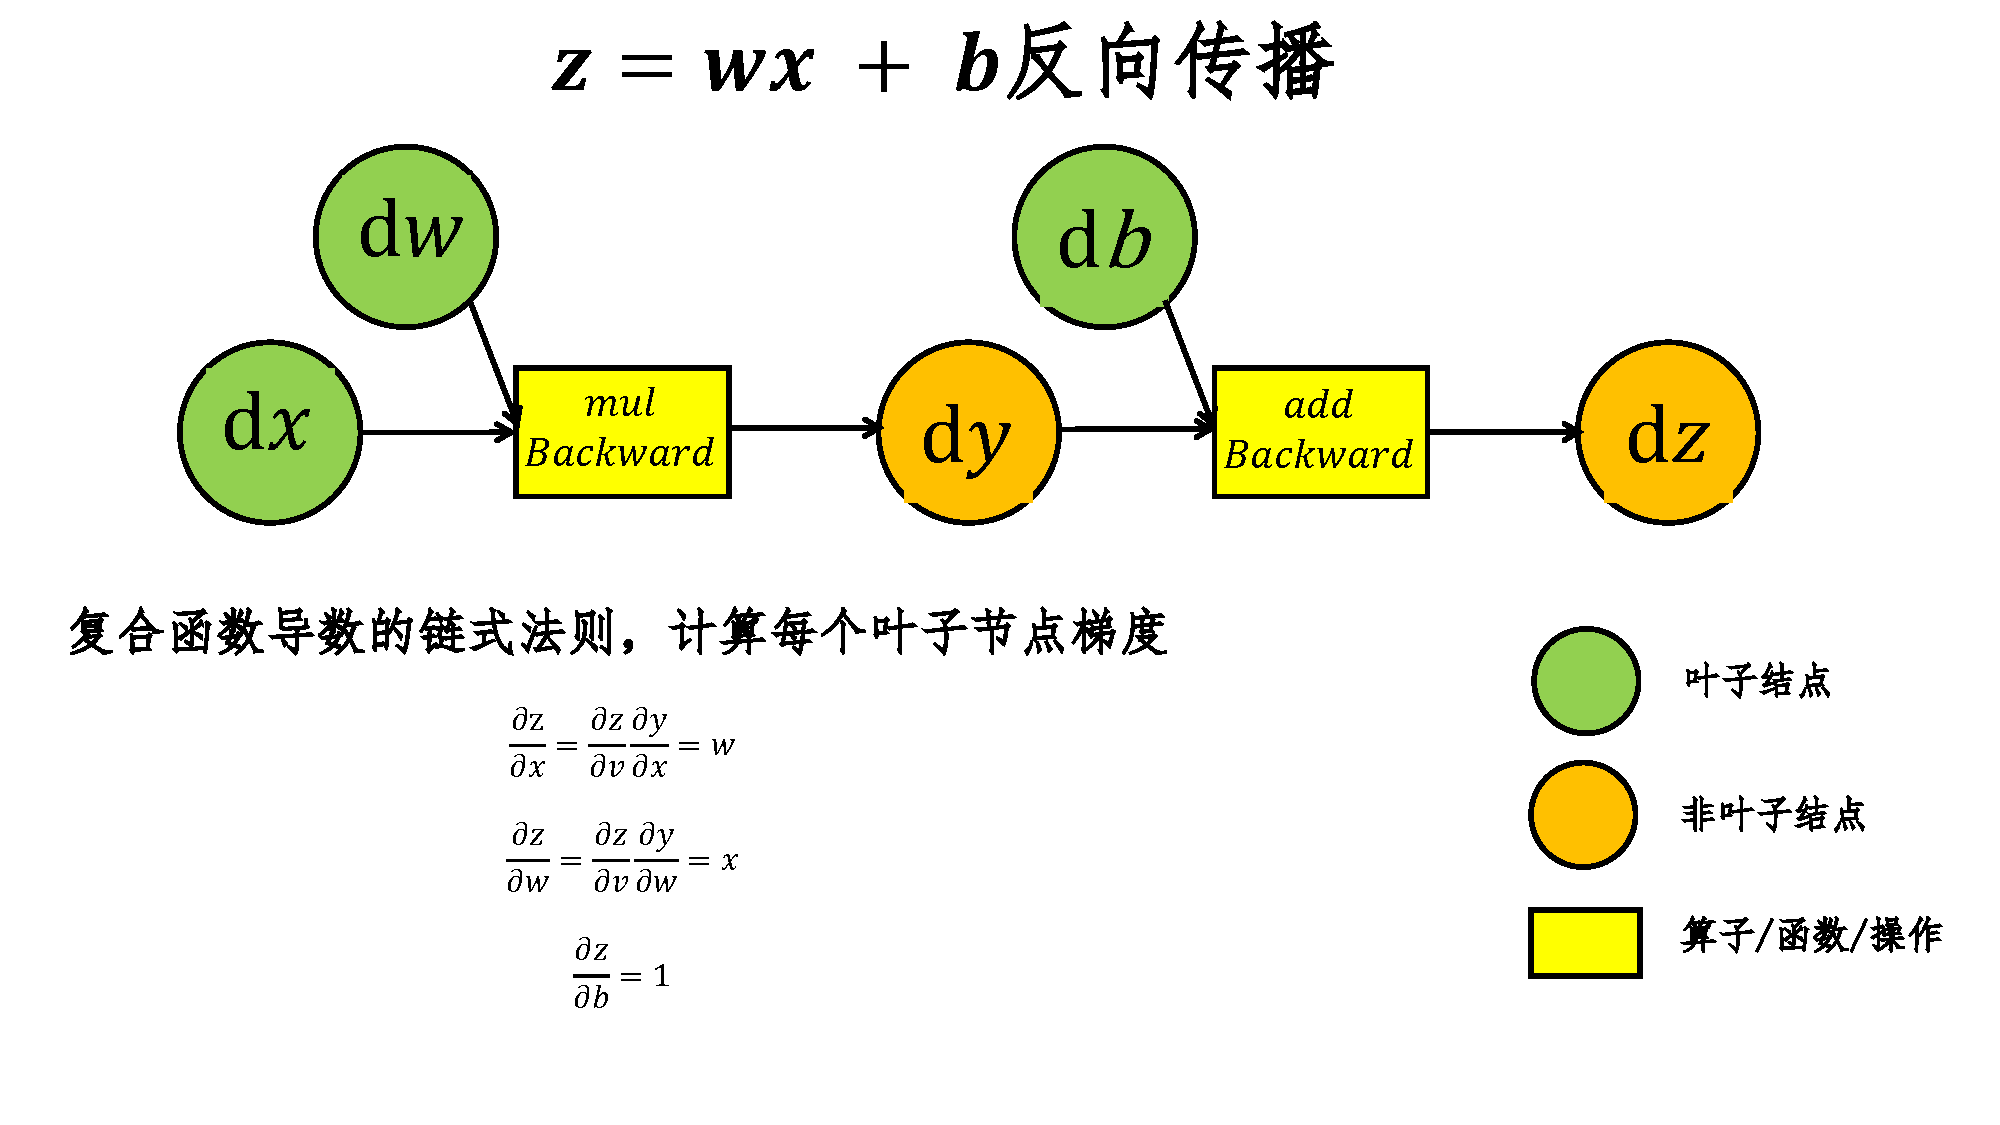
\includegraphics[width=0.5\textwidth]{part/人工智能/深度学习框架/pic/Pytorch/Pytorch基础/反向传播计算图.pdf}
    \caption{\label{fig:反向传播计算图}反向传播计算图}
    \end{minipage}
    \caption{\label{fig:前向传播和反向传播计算图}前向传播和反向传播计算图}
    \end{figure}

    图\ref{fig:反向传播计算图}所示,我们的目标是\textcolor{YBXPurple}{更新各叶子节点的梯度}，
    根据复合函数导数的链式法则，不难算出各叶子节点的梯度。

    $$\begin{aligned}
            \frac{\partial z}{\partial x}&=\frac{\partial z}{\partial y}\frac{\partial y}{\partial x}=w\\
            \frac{\partial z}{\partial w}&=\frac{\partial z}{\partial y}\frac{\partial y}{\partial w}=x\\
            \frac{\partial z}{\partial b}&=1
            \end{aligned}$$

    PyTorch调用\codeinline{backward}函数自动计算各节点的梯度，
    这是一个反向传播过程。
    在反向传播过程中，\codeinline{autograd}沿着图\ref{fig:反向传播计算图},
    从当前根节点$z$反向溯源，利用导数链式法则，计算所有叶子节点的梯度，
    并将梯度值累加到\codeinline{grad}属性中。
\end{derivation}

对非叶子节点的计算操作(或function)记录在\codeinline{grad\_fn}属性中，
叶子节点的\codeinline{grad\_fn}值为\codeinline{None}。        

PyTorch使用自动微分的计算图的生命周期如图\ref{fig:PyTorch计算图的生命周期}所示，
PyTorch中的计算图是动态计算图，
动态计算图有两个特点：
\begin{enumerate}[label=\arabic*)]
        \item 正向传播是立即执行的;
        \item 反向传播后计算图立即销毁。
\end{enumerate}

\begin{figure}[htpb]
        \centering
        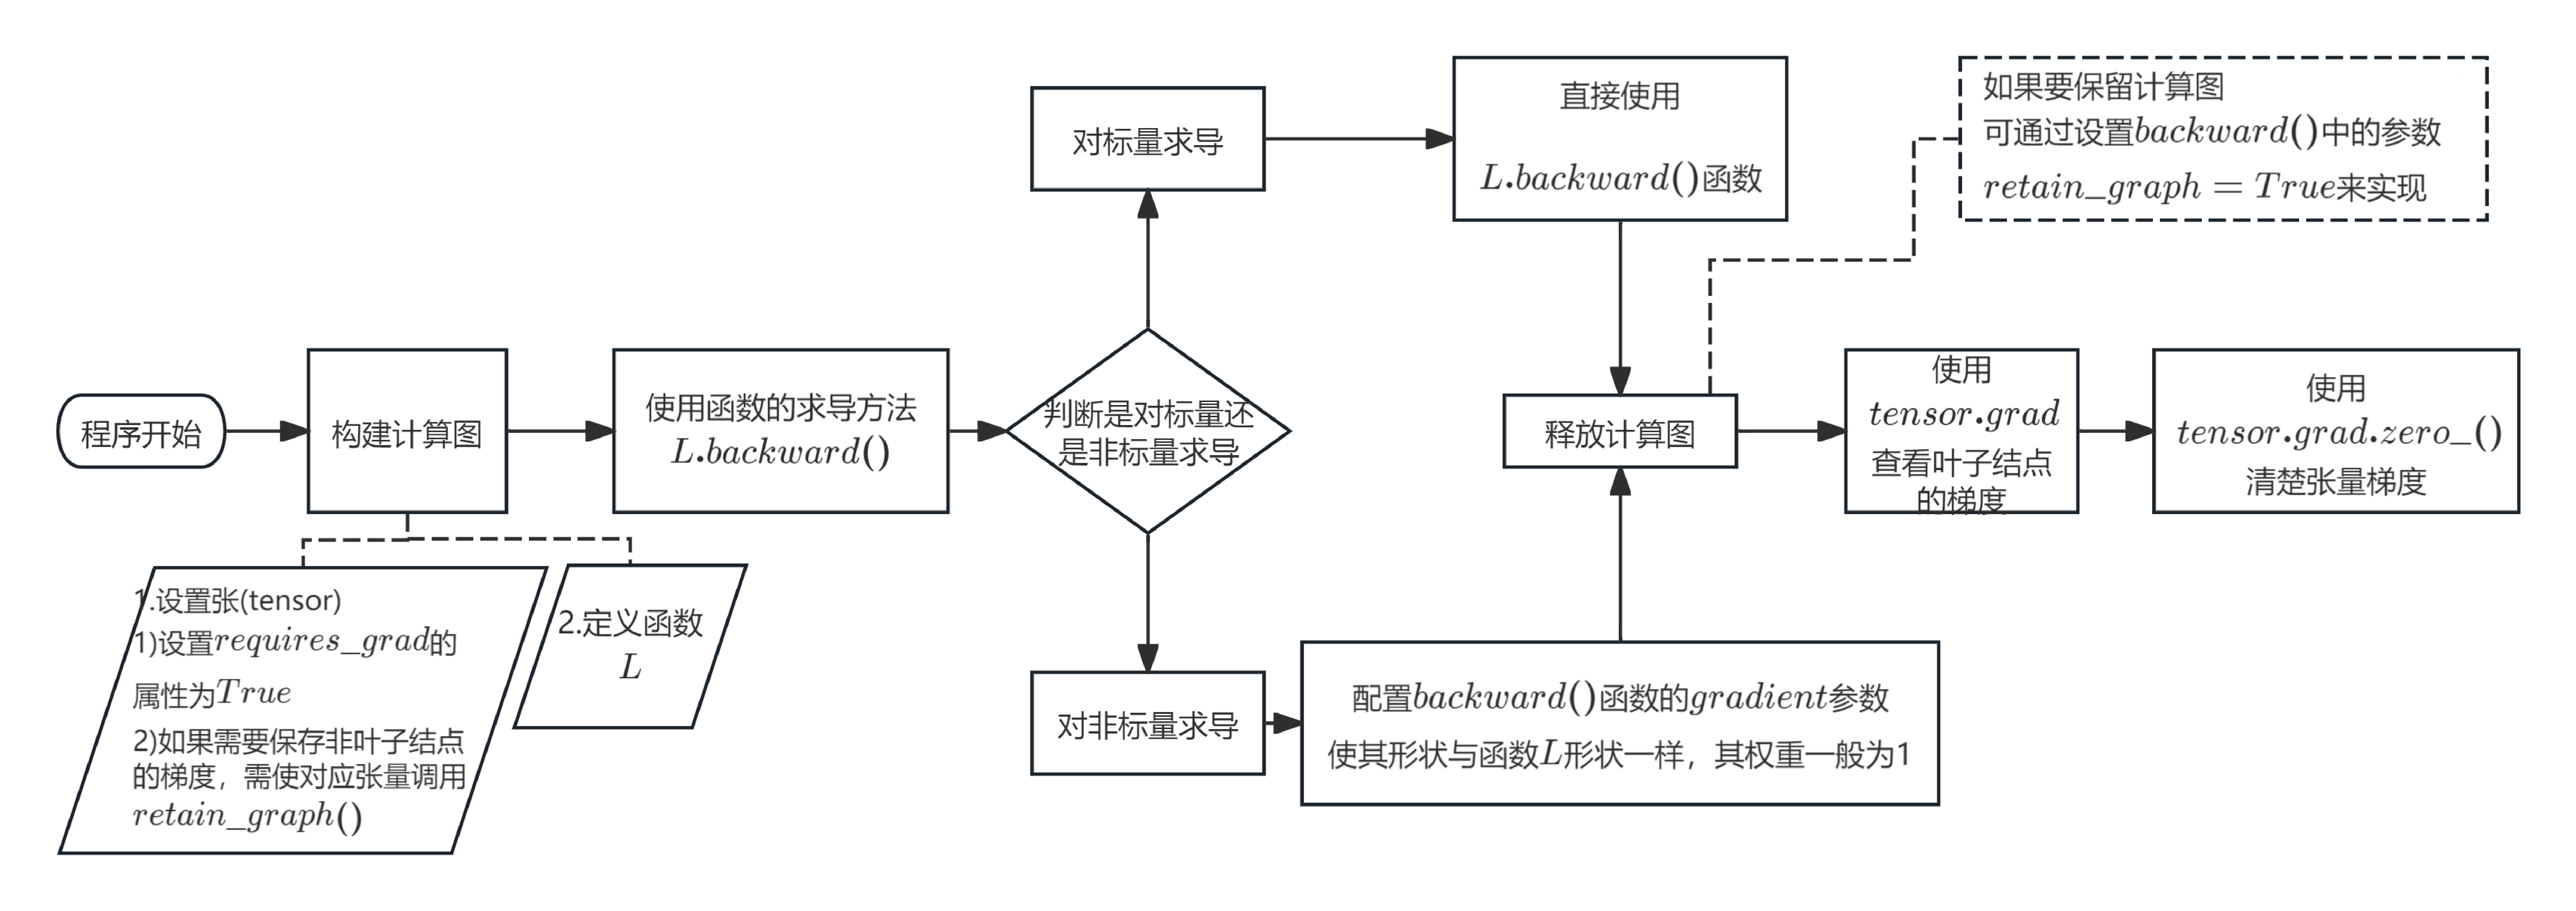
\includegraphics[width=0.8\textwidth]{part/人工智能/深度学习框架/pic/Pytorch/Pytorch基础/PyTorch计算图的生命周期.pdf}
        \caption{PyTorch计算图的生命周期}
        \label{fig:PyTorch计算图的生命周期}
\end{figure}

\begin{example}
    \exProblem
    用计算图表示 $y = (x + w) \times (w + 1)$，在$x =2, w = 1$ 时的计算图。
    \exSolution
    
    令$\left\{\begin{matrix}

        \begin{aligned}
        a &= x + w\\
        b &= w + 1\\
        y &= a \times b
        \end{aligned}
        \end{matrix}\right.$

    表示成有向无环图如图\ref{fig:计算图例题演示}所示。

    \begin{figure}[htpb]
        \centering
        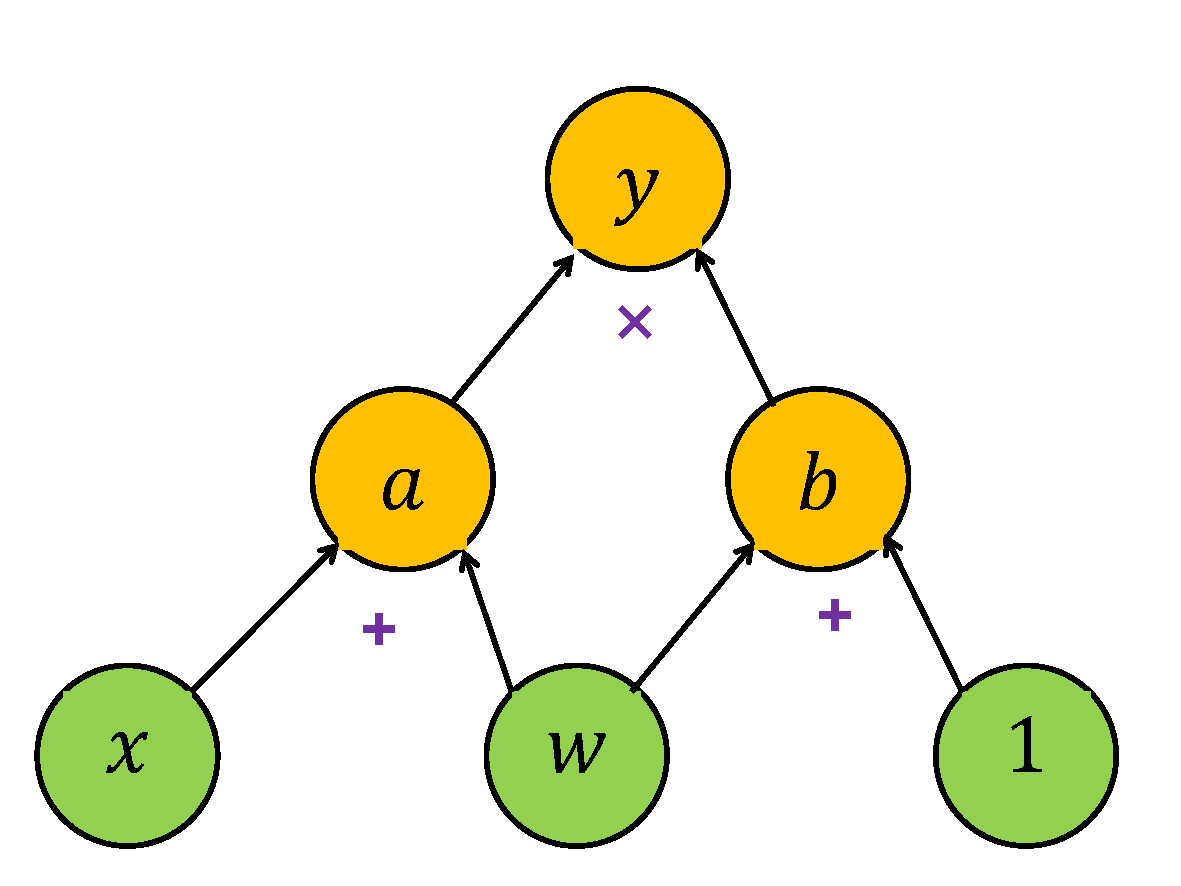
\includegraphics[width=0.4\textwidth]{part/人工智能/深度学习框架/pic/Pytorch/Pytorch基础/计算图例题演示.pdf}
        \caption{计算图例题演示}
        \label{fig:计算图例题演示}
    \end{figure}

    带入$x = 2, w = 1$，计算$y$的值，就是前向传播的过程。

    \begin{figure}[htpb]
        \centering
        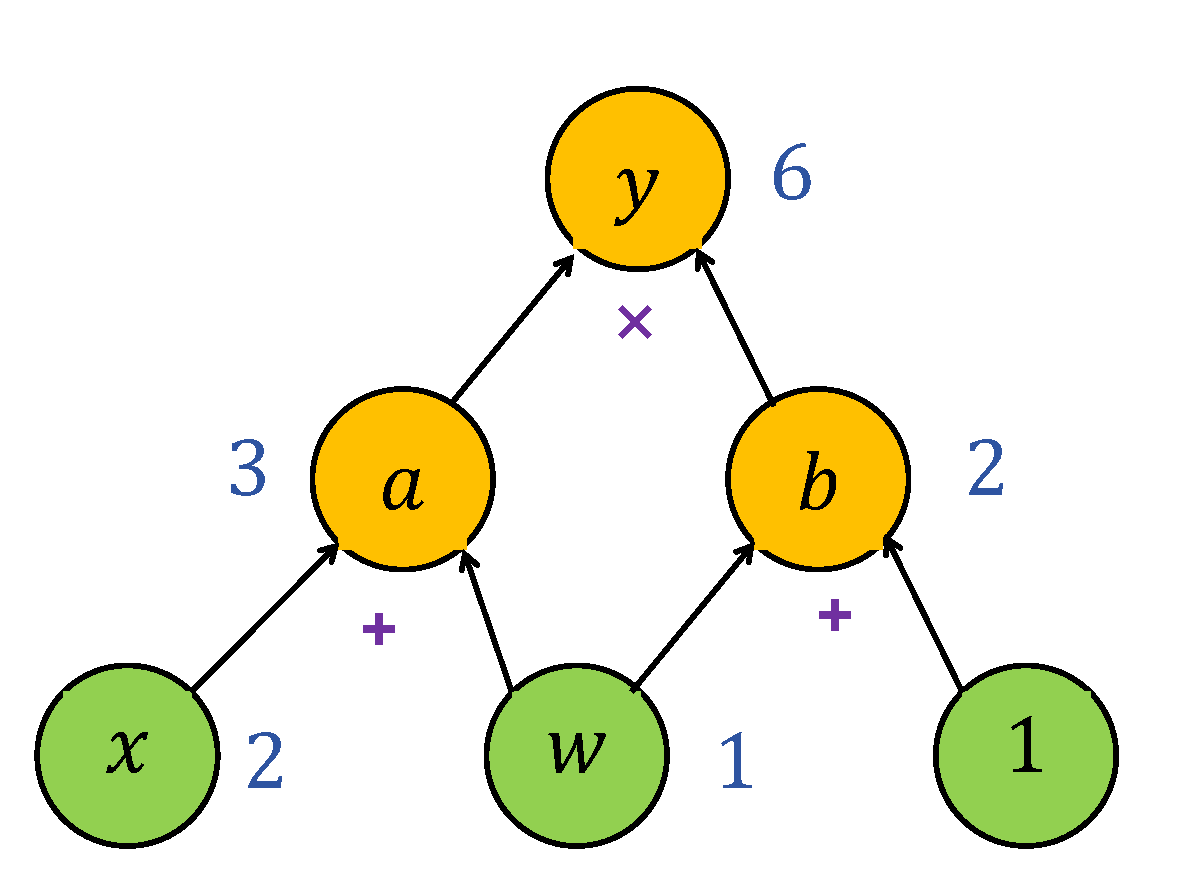
\includegraphics[width=0.4\textwidth]{part/人工智能/深度学习框架/pic/Pytorch/Pytorch基础/计算图例题演示-前向传播.pdf}
        \caption{计算图例题演示-前向传播}
        \label{fig:计算图例题演示-前向传播}
    \end{figure}

    $y$对$w$计算偏导
    $$\begin{aligned}
        \frac{\partial y}{\partial w}& = \frac{\partial y}{\partial a} \frac{\partial a}{\partial w} + \frac{\partial y}{\partial b} \frac{\partial b}{\partial w} \\
        &=b\times1+a\times1 \\
        &=b+a \\
        &= (w + 1) + (x + w) \\
        &=2*w+x+1 \\
        &=2\star1+2+1=5
        \end{aligned}$$

    \begin{figure}[htpb]
        \centering
        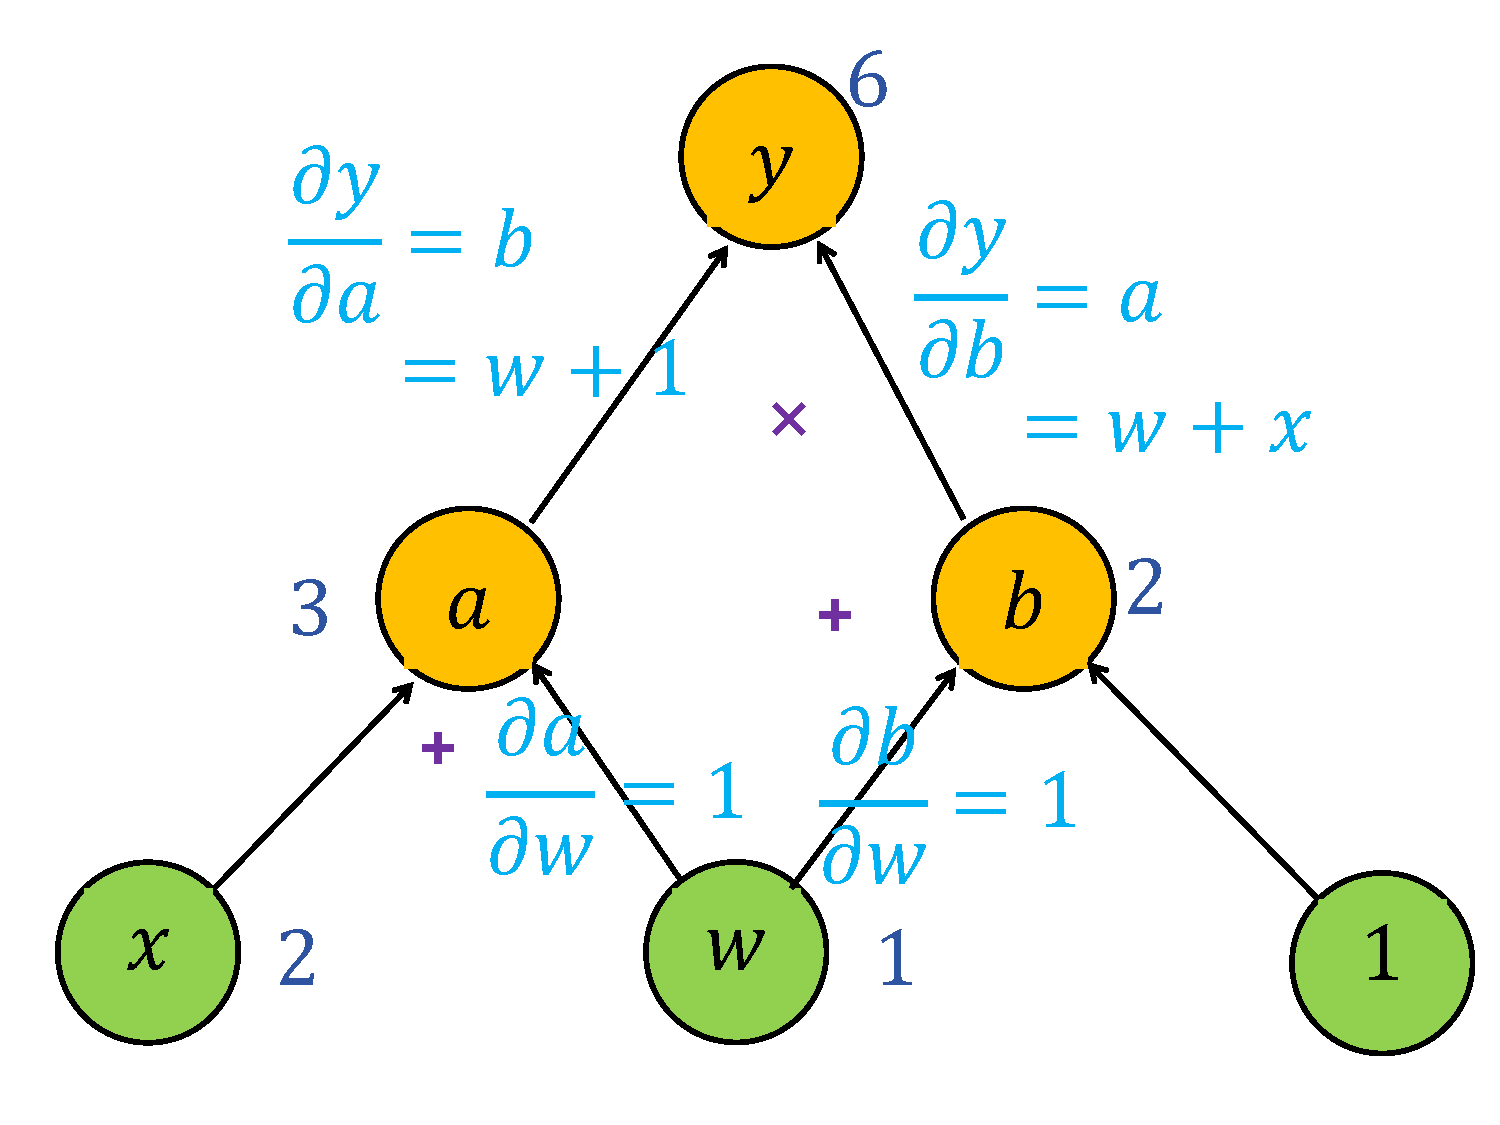
\includegraphics[width=0.4\textwidth]{part/人工智能/深度学习框架/pic/Pytorch/Pytorch基础/计算图例题演示-y对w求梯度.pdf}
        \caption{计算图例题演示-y对w求梯度}
        \label{fig:计算图例题演示-y对w求梯度}
    \end{figure}
    
    用代码实现如下：
    \begin{lstlisting}[style=pythonstyle]
    import torch

    w = torch.tensor([1.0], requires_grad=True)  # 初始化权重 w
    x = torch.tensor([2.0], requires_grad=True)  # 初始化输入 x
    
    a = torch.add(w, x)  # retain_grad() 保留梯度
    b = torch.add(w, 1)
    y = torch.mul(a, b)  # 计算 y
    
    y.backward()  # 反向传播
    print("y 对 w 的梯度：", w.grad)  # 输出 y 对 w 的梯度
    \end{lstlisting}
    \begin{lstlisting}[style=demostyle,numbers=none]
    y 对 w 的梯度： tensor([5.])
    \end{lstlisting}

    同理，$y$对$x$的梯度为
    $$\begin{aligned}
        \frac{\partial y}{\partial x}& = \frac{\partial y}{\partial a} \frac{\partial a}{\partial x} \\
        &=b\times1 \\
        &=b \\
        &=w+1 \\
        &=1+1=2
        \end{aligned}$$
    
    \begin{figure}[htpb]
        \centering
        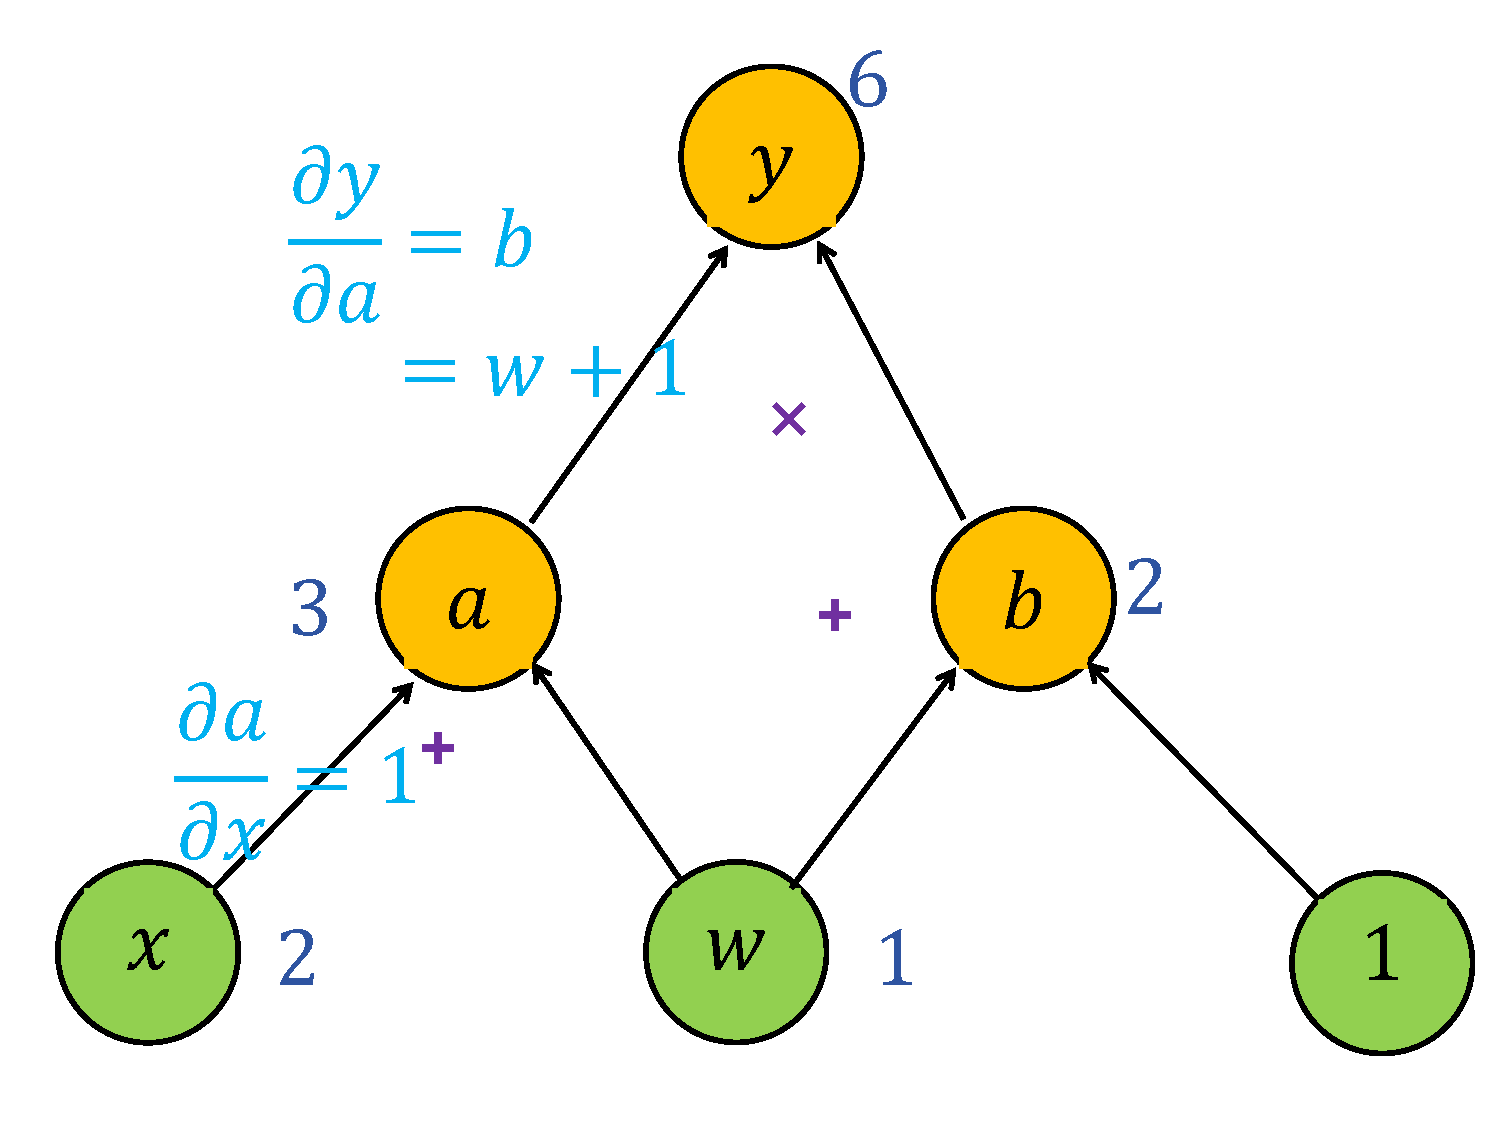
\includegraphics[width=0.4\textwidth]{part/人工智能/深度学习框架/pic/Pytorch/Pytorch基础/计算图例题演示-y对x求梯度.pdf}
        \caption{计算图例题演示-y对x求梯度}
        \label{fig:计算图例题演示-y对x求梯度}
    \end{figure}
        
    用代码实现如下：
    \begin{lstlisting}[style=pythonstyle]
    import torch

    w = torch.tensor([1.0], requires_grad=True)  # 初始化权重 w
    x = torch.tensor([2.0], requires_grad=True)  # 初始化输入 x
    
    a = torch.add(w, x)  # retain_grad() 保留梯度
    b = torch.add(w, 1)
    y = torch.mul(a, b)  # 计算 y
    
    y.backward()  # 反向传播
    print("y 对 w 的梯度：", w.grad)  # 输出 y 对 w 的梯度
    print("y 对 x 的梯度：", x.grad)  # 输出 y 对 x 的梯度
    \end{lstlisting}
    \begin{lstlisting}[style=demostyle,numbers=none]
    y 对 w 的梯度： tensor([5.])
    y 对 x 的梯度： tensor([2.])
    \end{lstlisting}
\end{example}

\subsubsection{计算图的元素}
\label{subsubsec:Pytorch的计算图的元素}
\begin{enumerate}[label=\arabic*)]
    \item 结点：

    结点表示\textcolor{YBXPurple}{数据}：向量、矩阵、张量等，
    
    结点有两种类型：
    \begin{enumerate}[itemindent=1em,label=\arabic*)]
        \item 叶子节点: 用户创建的变量，不依赖于其他变量。

        \item 非叶子节点：计算得到的变量，依赖于其他变量。
    \end{enumerate}

    只有叶子结点才有\textcolor{blue}{\textbf{梯度}}，梯度值保存在\codeinline{grad}属性中。
    \codeinline{requires\_grad}属性为\codeinline{True}。

    \begin{lstlisting}[style=pythonstyle]
    import torch

    w = torch.tensor([1.0], requires_grad=True)  # 初始化权重 w
    x = torch.tensor([2.0], requires_grad=True)  # 初始化输入 x

    a = torch.add(w, x)  # retain_grad() 保留梯度
    b = torch.add(w, 1)
    y = torch.mul(a, b)  # 计算 y

    # 查看是否是叶子节点
    print("w 是否是叶子节点：", w.is_leaf, "梯度为：", w.grad)
    print("x 是否是叶子节点：", x.is_leaf, "梯度为：", x.grad)
    print("a 是否是叶子节点：", a.is_leaf, "梯度为：", a.grad)
    print("b 是否是叶子节点：", b.is_leaf, "梯度为：", b.grad)
    print("y 是否是叶子节点：", y.is_leaf, "梯度为：", y.grad)
    \end{lstlisting}
    \begin{lstlisting}[style=demostyle,numbers=none]
    w 是否是叶子节点： True 梯度为： tensor([5.])
    x 是否是叶子节点： True 梯度为： tensor([2.])
    # 非叶子结点在反向传播结束后梯度会被自动清空
    a 是否是叶子节点： False 梯度为： None 
    b 是否是叶子节点： False 梯度为： None
    y 是否是叶子节点： False 梯度为： None
    \end{lstlisting}

    非叶子结点在反向传播结束后梯度会被自动清空。
    如果希望保留非叶子节点的梯度，可以使用\codeinline{retain\_grad()}方法。
    \begin{lstlisting}[style=pythonstyle]
    import torch

    w = torch.tensor([1.0], requires_grad=True)  # 初始化权重 w
    x = torch.tensor([2.0], requires_grad=True)  # 初始化输入 x
    
    a = torch.add(w, x)  # retain_grad() 保留梯度
    a.retain_grad()
    b = torch.add(w, 1)
    y = torch.mul(a, b)  # 计算 y
    
    y.backward()  # 反向传播
    
    
    # 查看是否是叶子节点
    print("w 是否是叶子节点：", w.is_leaf, "梯度为：", w.grad)
    print("x 是否是叶子节点：", x.is_leaf, "梯度为：", x.grad)
    print("a 是否是叶子节点：", a.is_leaf, "梯度为：", a.grad)
    print("b 是否是叶子节点：", b.is_leaf, "梯度为：", b.grad)
    print("y 是否是叶子节点：", y.is_leaf, "梯度为：", y.grad)
    \end{lstlisting}
    \begin{lstlisting}[style=demostyle,numbers=none]
    w 是否是叶子节点： True 梯度为： tensor([5.])
    x 是否是叶子节点： True 梯度为： tensor([2.])
    a 是否是叶子节点： False 梯度为： tensor([2.])
    b 是否是叶子节点： False 梯度为： None
    y 是否是叶子节点： False 梯度为： None
    \end{lstlisting}

    \item 边：

    边表示\textcolor{YBXPurple}{操作}：加法、乘法、激活函数等。
\end{enumerate}

\subsubsection{计算图的属性 grad\_fn}
\label{subsubsec:Pytorch的计算图的属性}
\codeinline{grad\_fn}属性表示该张量是通过什么操作得到的，
是一个\codeinline{Function}对象。

\codeinline{grad\_fn}的值：
\begin{enumerate}[label=\arabic*)]
    \item \textbf{None}：当一个张量是手动创建的
    
    例如使用 \codeinline{torch.tensor()} 或 \codeinline{torch.rand()}且没有参与任何需要自动求导的操作时，其 \codeinline{grad\_fn} 为 \codeinline{None}，这种张量被称为叶子节点（leaf tensor）。

    \item \textbf{AddBackward}：表示加法操作的反向传播函数。
    
    例如，\codeinline{z = x + y}，\codeinline{z.grad\_fn} 为 \codeinline{AddBackward}。

    \item \textbf{SubBackward}：表示减法操作的反向传播函数。
    
    例如，\codeinline{z = x - y}，\codeinline{z.grad\_fn} 为 \codeinline{SubBackward}。

    \item \textbf{MulBackward}：表示乘法操作的反向传播函数。
    
    例如，\codeinline{z = x * y}，\codeinline{z.grad\_fn} 为 \codeinline{MulBackward}。

    \item \textbf{DivBackward}：表示除法操作的反向传播函数。
    
    例如，\codeinline{z = x / y}，\codeinline{z.grad\_fn} 为 \codeinline{DivBackward}。

    \item \textbf{PowBackward}：表示幂运算的反向传播函数。
    
    例如，\codeinline{z = x.pow(2)}，\codeinline{z.grad\_fn} 为 \codeinline{PowBackward}。

    \item \textbf{MatMulBackward}：表示矩阵乘法操作的反向传播函数。
    
    例如，\codeinline{z = torch.matmul(x, y)} 或 \codeinline{z = x @ y}，\codeinline{z.grad\_fn} 为 \codeinline{MatMulBackward}。

    \item \textbf{MeanBackward}：表示求均值操作的反向传播函数。
    
    例如，\codeinline{z = x.mean()}，\codeinline{z.grad\_fn} 为 \codeinline{MeanBackward}。

    \item \textbf{SumBackward}：表示求和操作的反向传播函数。
    
    例如，\codeinline{z = x.sum()}，\codeinline{z.grad\_fn} 为 \codeinline{SumBackward}。

    \item \textbf{ExpBackward}：表示指数函数的反向传播函数。
    
    例如，\codeinline{z = x.exp()}，\codeinline{z.grad\_fn} 为 \codeinline{ExpBackward}。

    \item \textbf{SqrtBackward}：表示平方根函数的反向传播函数。
    
    例如，\codeinline{z = x.sqrt()}，\codeinline{z.grad\_fn} 为 \codeinline{SqrtBackward}。

    \item \textbf{LogBackward}：表示对数函数的反向传播函数。
    
    例如，\codeinline{z = x.log()}，\codeinline{z.grad\_fn} 为 \codeinline{LogBackward}。

    \item \textbf{TBackward}：表示转置操作的反向传播函数。
    
    例如，\codeinline{z = x.t()}（二维矩阵转置），\codeinline{z.grad\_fn} 为 \codeinline{TBackward}。

    \item \textbf{ReluBackward}：表示 ReLU 激活函数的反向传播函数。
    
    例如，\codeinline{z = torch.relu(x)}，\codeinline{z.grad\_fn} 为 \codeinline{ReluBackward}。

    \item \textbf{SigmoidBackward}：表示 Sigmoid 激活函数的反向传播函数。
    
    例如，\codeinline{z = torch.sigmoid(x)}，\codeinline{z.grad\_fn} 为 \codeinline{SigmoidBackward}。

    \item \textbf{ViewBackward}：表示视图操作（即张量视图转换）的反向传播函数。
    
    例如，\codeinline{z = x.view(-1)}，\codeinline{z.grad\_fn} 为 \codeinline{ViewBackward}。

    \item \textbf{CatBackward}：表示张量拼接操作的反向传播函数。
    
    例如，\codeinline{z = torch.cat((x, y), dim=0)}，\codeinline{z.grad\_fn} 为 \codeinline{CatBackward}。

    \item \textbf{CloneBackward}：表示克隆操作的反向传播函数。
    
    例如，\codeinline{z = x.clone()}，\codeinline{z.grad\_fn} 为 \codeinline{CloneBackward}。

    \item \textbf{IndexBackward}：表示索引操作的反向传播函数。
    
    例如，\codeinline{z = x[0]}，\codeinline{z.grad\_fn} 为 \codeinline{IndexBackward}。
\end{enumerate}

\begin{lstlisting}[style=pythonstyle]
import torch

w = torch.tensor([1.0], requires_grad=True)  # 初始化权重 w
x = torch.tensor([2.0], requires_grad=True)  # 初始化输入 x

a = torch.add(w, x)  # retain_grad() 保留梯度
a.retain_grad()
b = torch.add(w, 1)
y = torch.mul(a, b)  # 计算 y

y.backward()  # 反向传播


# 查看grad_fn
print("w.grad_fn: ", w.grad_fn)
print("x.grad_fn: ", x.grad_fn)
print("a.grad_fn: ", a.grad_fn)
print("b.grad_fn: ", b.grad_fn)
print("y.grad_fn: ", y.grad_fn)
\end{lstlisting}
\begin{lstlisting}[style=demostyle,numbers=none]
w.grad_fn:  None # 因为是叶子结点，所以没有grad_fn
x.grad_fn:  None
a.grad_fn:  <AddBackward0 object at 0x7fae3975ae60>
b.grad_fn:  <AddBackward0 object at 0x7fae43a57fa0>
y.grad_fn:  <MulBackward0 object at 0x7fae3975ae60>
\end{lstlisting}        

\subsection{autograd包}
\label{subsec:Pytorch的autograd包}
\subsubsection{torch.autograd 简介}
\begin{enumerate}[label=\arabic*)]
        \item 自动求导机制通过有向无环图（directed acyclic graph ，DAG）实现
        \item 在DAG中，记录数据（对应tensor.data）以及操作（对应tensor.grad\_fn）
        \item 操作在pytorch中统称为Function，
        如加法、减法、乘法、ReLU、conv、Pooling等，统统是Function  
\end{enumerate}

autograd的使用有很多方法，这里重点常用的
\begin{enumerate}[label=\arabic*)]
        \item \codeinline{torch.autograd.backward()}：自动求取梯度
        \item \codeinline{torch.autograd.grad()}：求取梯度
        \item \codeinline{torch.autograd.Function}：自定义Function
\end{enumerate}


\subsubsection{torch.autograd.backward()}
\label{subsubsec:Pytorch的torch.autograd.backward()}
PyTorch提供了\codeinline{torch.autograd.backward()}函数用于实现自动求取梯度。

\begin{lstlisting}[style=demostyle, numbers=none]
# 功能：实现自动求取梯度
torch.autograd.backward(
    tensors,                # 用于计算梯度的张量
    grad_tensors = None,    # 计算非标量的梯度。其形状一般与前面的张量保持一致。
    retain_graph=None,      # 由于PyTorch采用动态图机制,
                            # 在调用一次backward函数后PyTorch会自动销毁计算图
                            # 如果想对某个变量重复调用backward函数，则需要将该参数设置为True。
    create_graph=False,     # 创建导数计算图，用于高阶求导
                            # 当设置为True的时候可以用来计算更高阶的梯度。
    grad_variables=None     # 这个参数后面版本中应该会丢弃，直接使用grad_tensors就好了。
)  
\end{lstlisting}

\textcolor{red}{\textbf{注意}}：我们使用时候都是在张量上直接调用\codeinline{.backward()}函数，
但这里却是\codeinline{torch.autograd.backward}，为什么不一样呢？ 
其实\codeinline{Tensor.backward()}接口内部调用了\codeinline{autograd.backward}。

\begin{enumerate}[label=\arabic*)]
    \item \codeinline{retain\_grad}参数使用：
    \begin{lstlisting}[style=pythonstyle]
    #####  retain_graph=True
    import torch
    w = torch.tensor([1.], requires_grad=True)
    x = torch.tensor([2.], requires_grad=True)
    
    a = torch.add(w, x)
    b = torch.add(w, 1)
    y = torch.mul(a, b)  
    
    y.backward(retain_graph=True)
    print(w.grad)
    y.backward()
    print(w.grad) 
    \end{lstlisting} 
    \begin{lstlisting}[style=demostyle,numbers=none]
    tensor([5.])
    tensor([10.])
    \end{lstlisting}

    \begin{lstlisting}[style=pythonstyle]
    #####  retain_graph=False
    import torch
    w = torch.tensor([1.], requires_grad=True)
    x = torch.tensor([2.], requires_grad=True)

    a = torch.add(w, x)
    b = torch.add(w, 1)
    y = torch.mul(a, b)

    y.backward()
    print(w.grad)
    y.backward()
    print(w.grad)
    \end{lstlisting}
    \begin{lstlisting}[style=demostyle,numbers=none]
    tensor([5.])
    ---------------------------------------------------------------------------
    RuntimeError                              Traceback (most recent call last)
    <ipython-input-9-64bccc64184d> in <module>
        10 y.backward()
        11 print(w.grad)
    ---> 12 y.backward()
        13 print(w.grad)
    RuntimeError: Trying to backward through the graph a second time (or directly access saved tensors after they have already been freed). Saved intermediate values of the graph are freed when you call .backward() or autograd.grad(). Specify retain_graph=True if you need to backward through the graph a second time or if you need to access saved tensors after calling backward.
    \end{lstlisting}

    \item \codeinline{grad\_tensors}参数使用：
    \begin{lstlisting}[style=pythonstyle]
    w = torch.tensor([1.], requires_grad=True)
    x = torch.tensor([2.], requires_grad=True)
    
    a = torch.add(w, x)     
    b = torch.add(w, 1)
    
    y0 = torch.mul(a, b)    # y0 = (x+w) * (w+1)    dy0/dw = 2w + x + 1
    y1 = torch.add(a, b)    # y1 = (x+w) + (w+1)    dy1/dw = 2
    
    loss = torch.cat([y0, y1], dim=0)       # [y0, y1]
    
    grad_tensors = torch.tensor([1., 2.])
    
    loss.backward(gradient=grad_tensors)    # Tensor.backward中的 gradient 传入 torch.autograd.backward()中的grad_tensors
    
    # w =  1* (dy0/dw)  +   2*(dy1/dw)
    # w =  1* (2w + x + 1)  +   2*(w)
    # w =  1* (5)  +   2*(2)
    # w =  9
    
    print(w.grad)
    \end{lstlisting}
    \begin{lstlisting}[style=demostyle,numbers=none]
    tensor([9.])
    \end{lstlisting}
\end{enumerate}


\begin{example}
        \exProblem
        令$\left\{\begin{matrix}
        \begin{aligned}
        a=w+x \\
        b=w+1
        \end{aligned}
        \end{matrix}\right.$, $\left\{\begin{matrix}
        \begin{aligned}
        y_0&=a\times b = w^2+ w + wx+ x\\
        y_1&=a+b =  2w + x +1
        \end{aligned}
        \end{matrix}\right.$
        
        假定计算在$w=1, x=2$时的梯度

        当$grad f= \nabla f_{loss} = (\frac{\partial f}{\partial y_0},\frac{\partial f}{\partial y_1}) = (1,2)$,计算$w$的梯度$w.grad$

        当$\nabla f_{loss} = (3,4)$,计算$w$的梯度$w.grad$

        \exSolution
        \begin{enumerate}[label=\arabic*)]
                \item 当$\nabla f_{loss} = (1,2)$
                \begin{enumerate}[itemindent=1em,label=(\arabic*)]
                        \item 计算在$w=1, x=2$时的$y_0, y_1$的值
                        $$\left\{\begin{matrix}
                                \begin{aligned}
                                y_0=a\times b=(x+w)\times(w+1) = (2 + 1)\times(1 + 1)=6 \\
                                y_1=a+b= (x+w)+(w+1) = (2 + 1)+(1 + 1)=5 
                                \end{aligned}
                                \end{matrix}\right.
                                $$
                        \item 构造损失函数
                        因为在进行反向传播时，通常会对损失函数（loss）进行求导，以获得各个参数的梯度,因此定义函数$f_{loss}$
        
                        $$f_{loss} = f(y_0, y_1)$$
                        
                        上面的$f_{loss}$使用python实现如下
                        \begin{lstlisting}[style=pythonstyle]
                        loss = torch.cat([y_0​,y_1​],dim=0)=[6,5]
                        \end{lstlisting}
                        
                        $$\begin{aligned}
                        \frac{\partial y_0}{\partial w}&=\frac\partial{\partial w}\left[(x+w)\times(w+1)\right]\\
                        &=\frac\partial{\partial w}\left[(2+w)\times(1+w)\right] \\
                        &=(2+w)+(1+w)=3+2w 
                        \end{aligned}$$

                        当$w=1, \frac{\partial y_0}{\partial w}=3+2\times1=5$
                        
                        同理$\frac{\partial y_1}{\partial w}=\frac\partial{\partial w}\left[(x+w)+(w+1)\right]=1+1=2$

                        \item 调用\codeinline{backward()}函数计算梯度
                        当loss的梯度为$\nabla f_{loss} = (\frac{\partial\text{loss}}{\partial y_0}=1, \frac{\partial\text{loss}}{\partial y_1}=2)=(1, 2)$
        
                        上面赋值$\nabla f_{loss}$的代码如下：
                        \begin{lstlisting}[style=pythonstyle]
                        grad_tensors = torch.tensor([1., 2.])
                        loss.backward(gradient=grad_tensors)
                        \end{lstlisting}
                        
                        因此
                        $$
                        \begin{aligned}
                        w.\mathrm{grad}&=\frac{\partial\text{loss}}{\partial y_0}\times\frac{\partial y_0}{\partial w} +\frac{\partial\text{loss}}{\partial y_1}\times\frac{\partial y_1}{\partial w}\\
                        &=1\times 5 +2\times2\\
                        &=9
                        \end{aligned}
                        $$
                \end{enumerate}
                

                \item 当$\nabla f_{loss} = (3,4)$
                $$
                \begin{aligned}
                w.\mathrm{grad}&=3\times\frac{\partial y_0}{\partial w} +4\times\frac{\partial y_1}{\partial w}\\
                &=3\times 5 + 4\times2\\
                &=23
                \end{aligned}
                $$
        \end{enumerate}

        \begin{lstlisting}[style=pythonstyle,mathescape=true]
        import torch
        
        # 依赖于叶子节点的节点，requires_grad 默认为 True
        w = torch.tensor([1.], requires_grad=True)
        x = torch.tensor([2.] ,requires_grad=True)
        a = torch.add(w, x)
        b = torch.add(w, 1)
        
        y_0 = torch.mul(a, b)
        y_1 = torch.add(a, b)
        loss = torch.cat([y_0, y_1], dim=0)
        grad_tensors = torch.tensor([1., 2.])
        # loss.backward(gradient=grad_tensors) # 如果就计算1次
        # 当$\textcolor{DarkGreen}{\nabla f_{loss} = (1,2)}$时
        loss.backward(gradient=grad_tensors, retain_graph=True)
        print("w.grad:", w.grad)
        
        # 在设置 retain_graph=True 的情况下，可以多次调用 backward
        # 当$\textcolor{DarkGreen}{\nabla f_{loss} = (3,4)}$时
        # 梯度不能自动清零，在每次反向传播中会叠加
        w.grad.zero_()
        grad_tensors = torch.tensor([3., 4.])
        loss.backward(gradient=grad_tensors)
        print("w.grad:", w.grad)  
        \end{lstlisting}     
        \begin{lstlisting}[style=demostyle,numbers=none]
        w.grad: tensor([9.])
        w.grad: tensor([23.])          
        \end{lstlisting}
                        
\end{example}




\subsubsubsection{标量反向传播}
\label{subsubsec:Pytorch的标量反向传播}
\begin{lstlisting}[style=pythonstyle]
import torch
# 定义输入张量x 
x = torch.Tensor([3])

# 初始化权重参数w和偏置b，并设置 requires_grad=True 表示需要计算梯度
w = torch.randn(1, requires_grad=True) # 随机初始化一个权重参数
b = torch.randn(1, requires_grad=True) # 随机初始化一个偏置

print("初始化的权重:", w, "\n初始化的偏置:", b, "\n输入张量x:", x)
# 实现正向传播
y = torch.mul(w, x) # 等价于 y = w * x
z = torch.add(y, b) # 等价于 z = y + b

print("张量y:", y, "\n张量z:", z)
# 查看 x, w, b 的 requires_grad 属性
print("x, w, b 的 requires_grad 属性分别为:", x.requires_grad, w.requires_grad, b.requires_grad)

# 查看非叶子结点的 requires_grad 属性
## 因与w、b有依赖关系,故y、z的requires_grad属性也是：True、 True
print("y, z 的 requires_grad 属性分别为:", y.requires_grad, z.requires_grad)

# 查看个节点是否为叶子节点
print("x, w, b, y, z 是否为叶子结点:", x.is_leaf, w.is_leaf, b.is_leaf, y.is_leaf, z.is_leaf)

#查看叶子节点的grad_fn属性
print("x, w, b 的 grad_fn 属性分别为:", x.grad_fn, w.grad_fn, b.grad_fn)

# 查看非叶子结点的 grad_fn 属性
print("y, z 的 grad_fn 属性分别为:", y.grad_fn, z.grad_fn)

# 基于 z 张量进行梯度反向传播，执行backward()操作
z.backward()
# 如果需要多次使用backward函数，需要修改参数retain_graph为True,此时梯度是累加的
# z.backward(retain_graph=True)
#查看叶子节点的梯度，
# x是叶子节点但因为不需要更新，因此它无须求导,，故其梯度为None
print("各个叶子结点的梯度x, w, b 分别为:", x.grad, w.grad, b.grad)
# 非叶子节点的梯度，执行backward函数之后，会自动清空
print("非叶子结点的梯度:", y.grad, z.grad)
\end{lstlisting}
\begin{lstlisting}[style=demostyle,numbers=none]
初始化的权重: tensor([0.4014], requires_grad=True) 
初始化的偏置: tensor([-0.4248], requires_grad=True) 
输入张量x: tensor([3.])
张量y: tensor([1.2041], grad_fn=<MulBackward0>) 
张量z: tensor([0.7792], grad_fn=<AddBackward0>)
x, w, b 的 requires_grad 属性分别为: False True True
y, z 的 requires_grad 属性分别为: True True
x, w, b, y, z 是否为叶子结点: True True True False False
x, w, b 的 grad_fn 属性分别为: None None None
y, z 的 grad_fn 属性分别为: <MulBackward0 object at 0x7fc7a549f8e0> <AddBackward0 object at 0x7fc7a549f8b0>
各个叶子结点的梯度x, w, b 分别为: None tensor([3.]) tensor([1.])
非叶子结点的梯度: None None
\end{lstlisting}

如果需要多次使用\codeinline{backward}函数，需要修改参数\codeinline{retain\_graph}为\codeinline{True},此时梯度是累加的

\begin{lstlisting}[style=pythonstyle]
import torch

# 定义输入张量x 
x = torch.Tensor([2])

# 初始化权重参数w和偏置b，并设置 requires_grad=True 表示需要计算梯度
w = torch.randn(1, requires_grad=True)  # 随机初始化一个权重参数
b = torch.randn(1, requires_grad=True)  # 随机初始化一个偏置

print("初始化的权重:", w.item(), "\n初始化的偏置:", b.item(), "\n输入张量x:", x.item())

# 实现正向传播
y = torch.mul(w, x)  # 等价于 y = w * x
z = torch.add(y, b)  # 等价于 z = y + b

print("张量y:", y.item(), "\n张量z:", z.item())

# 查看 x, w, b 的 requires_grad 属性
print("x, w, b 的 requires_grad 属性分别为:", x.requires_grad, w.requires_grad, b.requires_grad)

# 查看非叶子结点的 requires_grad 属性
print("y, z 的 requires_grad 属性分别为:", y.requires_grad, z.requires_grad)

# 查看个节点是否为叶子节点
print("x, w, b, y, z 是否为叶子结点:", x.is_leaf, w.is_leaf, b.is_leaf, y.is_leaf, z.is_leaf)

# 查看叶子节点的grad_fn属性
print("x, w, b 的 grad_fn 属性分别为:", x.grad_fn, w.grad_fn, b.grad_fn)

# 查看非叶子结点的 grad_fn 属性
print("y, z 的 grad_fn 属性分别为:", y.grad_fn, z.grad_fn)

# 第一次反向传播
print("\n==========================================================")
z.backward(retain_graph=True) 
# 如果需要多次使用backward函数，需要修改参数retain_graph为True,此时梯度是累加的
print("第一次反向传播后各个结点的值x, w, b, y, z分别为:", x.item(), w.item(), b.item(), y.item(), z.item())
print("第一次反向传播后各个叶子结点的梯度 x, w, b 分别为:", x.grad, w.grad.item(), b.grad.item())
print("第一次反向传播后非叶子结点的梯度 y, z:", y.grad, z.grad)

# 第二次反向传播
print("\n==========================================================")
z.backward(retain_graph=True)
print("第二次反向传播后各个结点的值x, w, b, y, z分别为:", x.item(), w.item(), b.item(), y.item(), z.item())
print("第二次反向传播后各个叶子结点的梯度 x, w, b 分别为:", x.grad, w.grad.item(), b.grad.item())
print("第二次反向传播后非叶子结点的梯度 y, z:", y.grad, z.grad)

# 第三次反向传播
print("\n==========================================================")
z.backward()
print("第三次反向传播后各个结点的值x, w, b, y, z分别为:", x.item(), w.item(), b.item(), y.item(), z.item())
print("第三次反向传播后各个叶子结点的梯度 x, w, b 分别为:", x.grad, w.grad.item(), b.grad.item())
print("第三次反向传播后非叶子结点的梯度 y, z:", y.grad, z.grad)
\end{lstlisting}
\begin{lstlisting}[style=demostyle,numbers=none]
初始化的权重: -0.74216628074646 
初始化的偏置: -0.9749470949172974 
输入张量x: 2.0
张量y: -1.48433256149292 
张量z: -2.4592795372009277
x, w, b 的 requires_grad 属性分别为: False True True
y, z 的 requires_grad 属性分别为: True True
x, w, b, y, z 是否为叶子结点: True True True False False
x, w, b 的 grad_fn 属性分别为: None None None
y, z 的 grad_fn 属性分别为: <MulBackward0 object at 0x7fc7a5337eb0> <AddBackward0 object at 0x7fc7a5337ee0>

==========================================================
第一次反向传播后各个结点的值x, w, b, y, z分别为: 2.0 -0.74216628074646 -0.9749470949172974 -1.48433256149292 -2.4592795372009277
第一次反向传播后各个叶子结点的梯度 x, w, b 分别为: None 2.0 1.0
第一次反向传播后非叶子结点的梯度 y, z: None None

==========================================================
第二次反向传播后各个结点的值x, w, b, y, z分别为: 2.0 -0.74216628074646 -0.9749470949172974 -1.48433256149292 -2.4592795372009277
第二次反向传播后各个叶子结点的梯度 x, w, b 分别为: None 4.0 2.0 
# 这里的梯度是在上一次的基础上累加的，因此就是2倍
第二次反向传播后非叶子结点的梯度 y, z: None None

==========================================================
第三次反向传播后各个结点的值x, w, b, y, z分别为: 2.0 -0.74216628074646 -0.9749470949172974 -1.48433256149292 -2.4592795372009277
第三次反向传播后各个叶子结点的梯度 x, w, b 分别为: None 6.0 3.0
第三次反向传播后非叶子结点的梯度 y, z: None None
\end{lstlisting}

\subsubsubsection{非标量反向传播}
\label{subsubsec:Pytorch的非标量反向传播}
\begin{enumerate}[label=\arabic*)]
        \item 一阶偏导，梯度

        对于非标量的反向传播，
        不能直接使用\codeinline{backward()}函数，
        $Y$为一个向量，我们想办法把这个向量转变成一个标量不就好了？比如我们可以对 $Y$求和
        然后用求和得到的标量对$X$求导，这样不会对结果有影响，例如：
        $$Y_{\mathrm{sum}}=\sum y_{i}=x_{1}^{2}+x_{2}^{2}+6$$
        $$\frac{\partial Y_{sum}}{\partial x_{1}}=2x_{1},\frac{\partial Y_{sum}}{\partial x_{2}}=2x_{2}$$

        实际上，对$Y$求和等价于$Y$点积一个全为1的向量或矩阵。
        这个向量矩阵$V$也就是我们需要传人的 \codeinline{grad\_tensors} 参数。
        (点积只是相对于一维向量而言的，对于矩阵或更高维的张量，可以看作对每一个维度做点积运算。)

        \begin{lstlisting}[style=pythonstyle]
        import torch
        X = torch.ones(2, requires_grad=True)
        print("X:", X)
        Y = X**2 + 3 
        print("Y:", Y)
        # Y.backward() # 因为Y非标量，报错
        Y.sum().backward()
        print("X.grad:", X.grad)
        \end{lstlisting}
        \begin{lstlisting}[style=demostyle,numbers=none]
        X: tensor([1., 1.], requires_grad=True)
        Y: tensor([4., 4.], grad_fn=<AddBackward0>)
        X.grad: tensor([2., 2.])
        \end{lstlisting}    

        \item Jacobian矩阵
        \begin{example}
                \exProblem
                我们先手工计算一下$y$对$x$的梯度，以验证 PyTorch 的 backward 函数的结果是否正确。$y$ 对$x$的梯度是一个雅可比矩阵，各项的值可通过以下方法进行计算。

                \exSolution
                假设$x=\left(x_{1}=2,x_{2}=3\right),y=\left(y_{1}=x_{1}^{2}+3x_{2},y_{2}=x_{2}^{2}+2x_{1}\right)$,不难得到        

                $$J=\begin{bmatrix}\frac{\partial y_1}{\partial x_1}&\frac{\partial y_1}{\partial x_2}\\\frac{\partial y_2}{\partial x_1}&\frac{\partial y_2}{\partial x_2}\end{bmatrix}=\begin{bmatrix}2x_1&3\\2&2x_2\end{bmatrix}$$
                $$J^{\mathrm{T}}\times\left[1,0\right]^{\mathrm{T}}=\left[\begin{matrix}\frac{\partial y_{1}}{\partial x_{1}}\\\frac{\partial y_{1}}{\partial x_{2}}\end{matrix}\right]$$
                $$J^{\mathrm{T}}\times\left[0,1\right]^{\mathrm{T}}=\left[\begin{matrix}\frac{\partial y_{2}}{\partial x_{1}}\\\frac{\partial y_{2}}{\partial x_{2}}\end{matrix}\right]$$

                当$x_1=2,x_2=3$时
                $$J=\begin{bmatrix}4&3\\2&6\end{bmatrix}$$

                所以 
                $$J^{T}=\begin{bmatrix}4&2\\3&6\end{bmatrix}$$

                由此可得
                $$J^{\mathrm{T}}\times\left[1,0\right]^{\mathrm{T}}=\left[\frac{\partial y_{1}}{\partial x_{1}}\right]=\left[\begin{matrix}4\\3\end{matrix}\right]$$
                $$J^{T}\times\left[0,1\right]^{T}=\begin{bmatrix}\frac{\partial y_{2}}{\partial x_{1}}\\\frac{\partial y_{2}}{\partial x_{2}}\end{bmatrix}=\begin{bmatrix}2\\6\end{bmatrix}$$
        \end{example}
        
        \begin{lstlisting}[style=pythonstyle]
        import torch

        # 定义叶子结点张量 x 形状为 1x2
        x = torch.tensor([[2.0, 3.0]],dtype=torch.float32, requires_grad=True)
        print("x:", x)

        # 初始化雅可比矩阵
        J = torch.zeros(2, 2)

        # 初始化目标张量，形状为 1x2
        y = torch.tensor([[1.0, 2.0]],dtype=torch.float32)
        print("初始化y:", y)

        # 定义 y 与 x 之间的映射关系
        y[0, 0] = x[0, 0] ** 2 + 3 * x[0, 1]
        y[0, 1] = x[0, 1] ** 2 + 2 * x[0, 0]
        print("定义之后的y:", y)

        ##############################################
        # 1.先让 v = (1, 0) 得到 y_1 对 x 的梯度
        # 需要重复使用 backward() 函数，因此需要设置 retain_graph=True
        y.backward(torch.tensor([[1.0, 0.0]]), retain_graph=True)
        J[0] = x.grad
        ## 因为 x.grad 是累加的，所以需要清零
        x.grad = torch.zeros_like(x.grad)
        print("y_1对x的梯度:", J[0])

        # 2.再让 v = (0, 1) 得到 y_2 对 x 的梯度
        y.backward(torch.tensor([[0.0, 1.0]]))
        J[1] = x.grad
        print("y_2对x的梯度:", J[1])

        # 输出雅可比矩阵
        print("雅可比矩阵J:", J)
        \end{lstlisting}
        \begin{lstlisting}[style=demostyle,numbers=none]
        x: tensor([[2., 3.]], requires_grad=True)
        初始化y: tensor([[1., 2.]])
        定义之后的y: tensor([[13., 13.]], grad_fn=<CopySlices>)
        y_1对x的梯度: tensor([4., 3.])
        y_2对x的梯度: tensor([2., 6.])
        雅可比矩阵J: tensor([[4., 3.],
                            [2., 6.]])  
        \end{lstlisting}  
        
        \textcolor{red}{\textbf{注意}}：这里的\codeinline{backward}函数的参数\codeinline{grad\_tensors}是一个向量，而不是一个标量。
        而且选取不对的\codeinline{grad\_tensors}会导致计算出的梯度不对。
        \begin{example}
                \exProblem
                如果$v = (1,1)$计算$y$对$x$的梯度，结果是多少？
                \exSolution
                $$J^{\mathrm{T}}\times\nu^{\mathrm{T}}=\begin{bmatrix}4&2\\3&6\end{bmatrix}\begin{bmatrix}1\\1\end{bmatrix}=\begin{bmatrix}6\\9\end{bmatrix}$$
        \end{example}
        
        \begin{lstlisting}[style=pythonstyle]
        import torch

        # 定义叶子结点张量 x 形状为 1x2
        x = torch.tensor([[2.0, 3.0]],dtype=torch.float32, requires_grad=True)
        print("x:", x)
        
        # 初始化目标张量，形状为 1x2
        y = torch.tensor([[1.0, 2.0]],dtype=torch.float32)
        print("初始化y:", y)
        
        # 定义 y 与 x 之间的映射关系
        y[0, 0] = x[0, 0] ** 2 + 3 * x[0, 1]
        y[0, 1] = x[0, 1] ** 2 + 2 * x[0, 0]
        print("定义之后的y:", y)
        
        y.backward(torch.tensor([[1.0, 1.0]]), retain_graph=True)
        print("y_1对x的梯度:", x.grad)
        \end{lstlisting}
        \begin{lstlisting}[style=demostyle,numbers=none]
        x: tensor([[2., 3.]], requires_grad=True)
        初始化y: tensor([[1., 2.]])
        定义之后的y: tensor([[13., 13.]], grad_fn=<CopySlices>)
        y_1对x的梯度: tensor([[6., 9.]])
        \end{lstlisting}
\end{enumerate}




\subsubsection{torch.autograd.grad()}
\label{subsubsec:Pytorch的torch.autograd.grad()}
PyTorch提供了\codeinline{torch.autograd.grad()}函数用于实现自动求取梯度。

\begin{lstlisting}[style=demostyle, numbers=none]
# 功能：实现自动求取梯度
torch.autograd.grad(
    outputs,                # 用于求导的张量
    inputs,                 # 需要梯度的张量
    grad_outputs=None,      # 计算非标量的梯度。其形状一般与前面的张量保持一致。
    retain_graph=None,      # 由于PyTorch采用动态图机制,
                            # 在调用一次backward函数后PyTorch会自动销毁计算图
                            # 如果想对某个变量重复调用backward函数，则需要将该参数设置为True。
    create_graph=False      # 创建导数计算图，用于高阶求导
                            # 当设置为True的时候可以用来计算更高阶的梯度。
    allow_unused=False      # 如果为True，即使某个输入张量的梯度未被使用，也不会报错
)  
\end{lstlisting}

其实\codeinline{torch.autograd.grad()}函数与\codeinline{torch.autograd.backward()}函数的功能类似，
\begin{enumerate}[label=\arabic*)]
        \item \codeinline{torch.autograd.backward()}函数是一个较为通用的函数，适用于计算损失函数相对于所有输入的梯度。
        \item \codeinline{torch.autograd.grad()}函数是一个更灵活的函数，允许用户指定计算哪些张量的梯度，并可以返回这些梯度，
        而不直接修改原始张量的 \codeinline{.grad} 属性。
\end{enumerate}

\begin{example}
        \exProblem
        $z = x \times y$,在$x=2, y=3$时，计算$\frac{\partial z}{\partial x}$和$\frac{\partial z}{\partial y}$
        \exSolution
        \begin{enumerate}[label=\arabic*)]
                \item 使用\codeinline{torch.autograd.grad()}函数计算
                \begin{lstlisting}[style=pythonstyle]
                import torch
        
                # 创建张量并设置 requires_grad=True
                x = torch.tensor([2.0], requires_grad=True)
                y = torch.tensor([3.0], requires_grad=True)
        
                # 定义一个简单的计算
                z = x * y  # z = 2.0 * 3.0 = 6.0
        
                # 调用 grad() 计算梯度
                grad_x, grad_y = torch.autograd.grad(outputs=z, inputs=[x, y])
        
                # 打印计算得到的梯度
                print("grad_x:", grad_x)  # 输出: tensor([3.])
                print("grad_y:", grad_y)  # 输出: tensor([2.])
                \end{lstlisting}
                \begin{lstlisting}[style=demostyle, numbers=none]
                grad_x: tensor([3.])
                grad_y: tensor([2.])
                \end{lstlisting}

                \item 使用\codeinline{torch.autograd.backward()}函数计算
                \begin{lstlisting}[style=pythonstyle]
                import torch

                # 创建张量并设置 requires_grad=True
                x = torch.tensor([2.0], requires_grad=True)
                y = torch.tensor([3.0], requires_grad=True)
                
                # 定义一个简单的计算
                z = x * y  # z = 2.0 * 3.0 = 6.0
                
                # 调用 backward() 计算梯度
                z.backward()
                
                # 打印 x 和 y 的梯度
                print("x.grad:", x.grad)  # 输出: tensor([3.])
                print("y.grad:", y.grad)  # 输出: tensor([2.])
                \end{lstlisting}  
                \begin{lstlisting}[style=demostyle, numbers=none]
                grad_x: tensor([3.])
                grad_y: tensor([2.])
                \end{lstlisting}                      
        \end{enumerate}
\end{example}




\subsubsection{torch.autograd.Function}
\label{subsubsec:Pytorch的torch.autograd.Function}
有的时候，想要实现自己的一些操作（op），如特殊的数学函数、pytorch的module中没有的网络层，
那就需要自己写一个Function，在Function中定义好\codeinline{forward}的计算公式、\codeinline{backward}的计算公式，
然后将这些op组合到模型中，模型就可以用\codeinline{autograd}完成梯度求取。

\begin{example}
    \exProblem
    假设需要一个计算指数的功能，并且能组合到模型中，实现autograd

    \begin{enumerate}[label=\arabic*)]
        \item 继承Function
        \item 实现forward和backward函数
    \end{enumerate}
    
    \exSolution
    \begin{enumerate}[label=\arabic*)]
        \item forward和backward函数第一个参数为\codeinline{ctx},
        它的作用类似于类函数的\codeinline{self}一样。

        \codeinline{ctx} 是一个上下文对象，具体为 context，它在自定义的 autograd 函数中用于在前向传播和反向传播之间共享信息。

        \begin{enumerate}[itemindent=1em,label=\arabic*)]
            \item 在 forward 中
            
            ctx 用来存储中间计算结果，供反向传播时使用。
            通过调用 \codeinline{ctx.save\_for\_backward} 可以将中间变量存储到 ctx 对象中（如代码中的 result）。
            \item 在 backward 中
            
            可以通过 \codeinline{ctx.saved\_tensors} 取出这些保存的变量，计算梯度。
            这是 PyTorch 提供的机制，确保在反向传播时能够获取到前向传播中的关键变量。
        \end{enumerate}
        
    
        \item backward函数返回的参数个数与forward的输入参数个数相同, 
        即，传入该op的参数，都需要给它们计算对应的梯度。
    \end{enumerate}
    \begin{lstlisting}[style=pythonstyle]
    import torch
    from torch.autograd.function import Function
    
    class Exp(Function):
        @staticmethod # 静态方法
        # 函数功能：计算输入 i 的指数值 i.exp()
        # ctx: 一个上下文对象，用于在 forward 和 backward 之间传递信息
        def forward(ctx, i):
            # ============== step1: 函数功能实现 ==============
            result = i.exp()
            # ============== step1: 函数功能实现 ==============
    
            # ============== step2: 结果保存，用于反向传播 ==============
            ctx.save_for_backward(result)
            # ============== step2: 结果保存，用于反向传播 ==============
    
            return result
        
        @staticmethod
        # 函数功能：计算梯度
        def backward(ctx, grad_output):
            # ============== step1: 取出结果，用于反向传播 ==============
            result, = ctx.saved_tensors
            # ============== step1: 取出结果，用于反向传播 ==============
    
    
            # ============== step2: 反向传播公式实现 ==============
            grad_results = grad_output * result
            # ============== step2: 反向传播公式实现 ==============
    
    
            return grad_results
    
    x = torch.tensor([1.], requires_grad=True)  
    # 前向传播
    y = Exp.apply(x)    # 需要使用apply方法调用自定义autograd function
                        # 继承 torch.autograd.Function 的类有一个静态方法 apply，
                        # 用于执行这个自定义的函数
                        # 调用 Exp.apply(x) 时，实际上是调用了 Exp 类的 forward 方法，这个方法实现了前向传播逻辑（即 i.exp()）。
                        # apply 的作用就是把输入张量传给 forward，同时构建计算图，并将其存储在 ctx 上，以便后续在 backward 中使用。
                        # 然后在反向传播阶段（调用 .backward() 时），backward 会根据前向传播时保存的信息来计算梯度。
    print(y)                                  #  y = e^x = e^1 = 2.7183
    # 反向传播
    y.backward()                            
    print(x.grad)                           # 反传梯度,  x.grad = dy/dx = e^x = e^1  = 2.7183
    \end{lstlisting}
    \begin{lstlisting}[style=demostyle, numbers=none]
    tensor([2.7183], grad_fn=<ExpBackward>)
    tensor([2.7183])
    \end{lstlisting}
\end{example}

\begin{example}
        \exProblem
        反向传梯度时乘以一个自定义系数
        \exSolution
        \begin{lstlisting}[style=pythonstyle]
        import torch
        from torch.autograd.function import Function
        
        class GradCoeff(Function):       
        
                @staticmethod
                # 函数功能：实现前向传播
                def forward(ctx, x, coeff):                 
        
                # ============== step1: 函数功能实现 ==============
                ctx.coeff = coeff   # 将coeff存为ctx的成员变量
                # ============== step1: 函数功能实现 ==============
                return x
        
                @staticmethod
                # 函数功能：为梯度乘以一定系数 ctx.coeff
                def backward(ctx, grad_output):            
                return ctx.coeff * grad_output, None    # backward的输出个数，应与forward的输入个数相同，此处coeff不需要梯度，因此返回None
        
        
        x = torch.tensor([2.], requires_grad=True)
        # 前向传播
        ret = GradCoeff.apply(x, -0.1)                  # 前向需要同时提供x及coeff，设置coeff为-0.1
        ret = ret ** 3                         
        print(ret)                                      # 注意看： ret.grad_fn 
        # 反向传播
        ret.backward()  
        print(x.grad)
        \end{lstlisting}
        \begin{lstlisting}[style=demostyle, numbers=none, mathescape=true]
        tensor([8.], grad_fn=<PowBackward0>)
        tensor([-1.2000])
        # $\textcolor{DarkGreen}{\frac{d(x^3)}{dx} = 3x^2}$
        # $\textcolor{DarkGreen}{x = 2}\Rightarrow \textcolor{DarkGreen}{\frac{d(2^3)}{dx} = 3 \times 2^2 = 12}$
        # $\textcolor{DarkGreen}{\text{grad} = -0.1 \times 12 = -1.2}$
        \end{lstlisting}
\end{example}

\begin{example}
        \exProblem
        手动实现2D卷积
        \exSolution
        \begin{lstlisting}[style=pythonstyle]
        import torch
        from torch.autograd.function import once_differentiable
        import torch.nn.functional as F

        def convolution_backward(grad_out, X, weight):
        """
        计算卷积操作的反向传播，返回两个梯度：输入张量X的梯度和卷积核weight的梯度
        参数：
        - grad_out: 前向传播的输出梯度
        - X: 输入张量
        - weight: 卷积核（权重）
        
        返回：
        - grad_X: 输入张量X的梯度
        - grad_weight: 卷积核weight的梯度
        """
        # 计算grad_input，即输入张量的梯度
        grad_input = F.conv2d(X.transpose(0, 1), grad_out.transpose(0, 1)).transpose(0, 1)
        # 计算grad_X，即权重的梯度
        grad_X = F.conv_transpose2d(grad_out, weight)
        return grad_X, grad_input

        class MyConv2D(torch.autograd.Function):
        @staticmethod
        def forward(ctx, X, weight):
                """
                前向传播：实现卷积操作
                参数：
                - ctx: 上下文对象，保存中间结果以供backward使用
                - X: 输入张量
                - weight: 卷积核（权重）
                
                返回：
                - ret: 卷积结果
                """
                # 保存输入张量X和卷积核weight，供反向传播使用
                ctx.save_for_backward(X, weight)

                # 使用PyTorch内置的conv2d函数进行卷积计算
                ret = F.conv2d(X, weight)
                return ret

        @staticmethod
        def backward(ctx, grad_out):
                """
                反向传播：计算卷积操作的梯度
                参数：
                - ctx: 上下文对象，获取前向传播保存的变量
                - grad_out: 前向传播输出的梯度
                
                返回：
                - 两个梯度：输入张量X的梯度和卷积核weight的梯度
                """
                # 从上下文中获取保存的X和weight
                X, weight = ctx.saved_tensors
                # 调用convolution_backward函数，计算并返回梯度
                return convolution_backward(grad_out, X, weight)

        # 初始化权重和输入张量
        weight = torch.rand(5, 3, 3, 3, requires_grad=True, dtype=torch.double)
        X = torch.rand(10, 3, 7, 7, requires_grad=True, dtype=torch.double)

        # 使用gradcheck来检查自定义操作的梯度计算是否正确
        # gradcheck会通过数值方法检查自定义操作是否实现了正确的梯度
        print("梯度检查: ", torch.autograd.gradcheck(MyConv2D.apply, (X, weight)))

        # 调用自定义的卷积操作
        y = MyConv2D.apply(X, weight)

        # 生成目标标签，计算损失
        label = torch.randn_like(y)
        loss = F.mse_loss(y, label)

        # 在反向传播前，打印weight的梯度，初始值为None
        print("反向传播前，weight.grad: ", weight.grad)

        # 反向传播，计算梯度
        loss.backward()

        # 打印反向传播后的weight梯度
        print("反向传播后，weight.grad: ", weight.grad)
        \end{lstlisting}
        \begin{lstlisting}[style=demostyle, numbers=none]
        梯度检查:  True
        反向传播前，weight.grad:  None
        反向传播后，weight.grad:  tensor([[[[1.3423, 1.3445, 1.3271],
                [1.3008, 1.3262, 1.2493],
                [1.2969, 1.3269, 1.2369]],
        ......
                [[1.2302, 1.2134, 1.2619],
                [1.2397, 1.2048, 1.2447],
                [1.2419, 1.2548, 1.2647]]]], dtype=torch.float64)        
        \end{lstlisting}
\end{example}


\subsection{autograd的注意事项}
\label{subsec:Pytorch的autograd的注意事项}
\subsubsection{梯度不会自动清零}
\label{subsubsec:Pytorch的梯度不会自动清零}
在PyTorch中，梯度不会自动清零，每次计算完梯度后，需要手动清零，否则会累加。

\begin{lstlisting}[style=pythonstyle]
import torch
w = torch.tensor([1.], requires_grad=True)
x = torch.tensor([2.], requires_grad=True)

for i in range(4):
    a = torch.add(w, x)
    b = torch.add(w, 1)
    y = torch.mul(a, b)

    y.backward()   
    print(w.grad)  # 梯度不会自动清零，数据会累加， 通常需要采用 optimizer.zero_grad() 完成对参数的梯度清零

#     w.grad.zero_()
\end{lstlisting}
\begin{lstlisting}[style=demostyle, numbers=none]
tensor([5.])
tensor([10.])
tensor([15.])
tensor([20.])
\end{lstlisting}

使用 \codeinline{w.grad.zero\_()} 可以手动将梯度清零，如下所示：
\begin{lstlisting}[style=pythonstyle]
import torch
w = torch.tensor([1.], requires_grad=True)
x = torch.tensor([2.], requires_grad=True)

for i in range(4):
    a = torch.add(w, x)
    b = torch.add(w, 1)
    y = torch.mul(a, b)

    y.backward()   
    print(w.grad)  # 输出累加的梯度

    # 手动将梯度清零
    w.grad.zero_()  
\end{lstlisting}
\begin{lstlisting}[style=demostyle, numbers=none]
tensor([5.])
tensor([5.])
tensor([5.])
tensor([5.])
\end{lstlisting}                        


\subsubsection{叶子结点不可执行in-place}
\label{subsubsec:Pytorch的叶子结点不可执行in-place}
叶子节点不可以执行in-place操作(\codeinline{torch.add\_}、
\codeinline{torch.mul\_}等)，否则会报错，如下所示：

\begin{lstlisting}[style=demostyle, numbers=none]
import torch
        
# 依赖于叶子节点的节点，requires_grad 默认为 True
w = torch.tensor([1.], requires_grad=True)
x = torch.tensor([2.] ,requires_grad=True)
a = torch.add(w, x)
b = torch.add(w, 1)

y = torch.mul(a, b)
w.add_(1.0)   
# RuntimeError: a leaf Variable that requires grad is being used in an in-place operation.
\end{lstlisting}

\subsubsection{detach 切断一些分支的反向传播}
\label{subsec:Pytorch的切断一些分支的反向传播}
训练网络时，有时候我们希望保持一部分的网络参数不变，
只对其中一部分的参数进行调整，只训练部分分支网络，
不让其梯度对主网络的梯度造成影响，这时候可以使用\codeinline{detach}。
函数来切断一些分支的反向传播。

\codeinline{detach\_()}将张量从创建它的计算图(Graph)中分离，
把它作为叶子节点，
其中参数\codeinline{grad\_fn = None} 且 \codeinline{requires\_grad = False}。

\begin{lstlisting}[style=pythonstyle]
import torch

# x = torch.ones(2, requires_grad=True)
x = torch.tensor([2., 2.], requires_grad=True)
# 对 x 每个元素*2
print("x:", x)
y = 2*x**3 + 4
print("y:", y)

## 对分离变量 y, 生成一个新的变量 c
c = y.detach()
print("c:", c)
z = c*x # 将此刻的 c 作为常数，不再参与梯度计算
print("z:", z)
print("z.sum():", z.sum())
z.sum().backward()

print("-------------------------")
# 对 c 进行反向传播
print("x.grad:", x.grad)
print("c.grad_fn:", c.grad_fn)
print("c.requires_grad:", c.requires_grad)

print("-------------------------")
x.grad.zero_()
y.sum().backward()
print("x.grad:", x.grad)
print("y.grad_fn:", y.grad_fn)
print("y.requires_grad:", y.requires_grad)
\end{lstlisting}
\begin{lstlisting}[style=demostyle,numbers=none]
x: tensor([2., 2.], requires_grad=True)
y: tensor([20., 20.], grad_fn=<AddBackward0>)
c: tensor([20., 20.])
z: tensor([40., 40.], grad_fn=<MulBackward0>)
z.sum(): tensor(80., grad_fn=<SumBackward0>)
-------------------------
x.grad: tensor([20., 20.])
c.grad_fn: None
c.requires_grad: False
-------------------------
x.grad: tensor([24., 24.])
y.grad_fn: <AddBackward0 object at 0x7f598a399870>
y.requires_grad: True
\end{lstlisting}  

\section{Tensor与Numpy比较}
\label{subsec:Pytorch的Tensor与Numpy比较}
PyTorch与NumPy有很多类似的地方，
并且有很多相同的操作函数名称，
所以有时很容易混淆，
下面我们对一些主要的区别进行汇总，具体可参考表\ref{tab:Pytorch_vs_NumPy}。
\begin{table}[h]
\centering
\resizebox{0.8\textwidth}{!}{
\begin{tabular}{|l|l|l|}
\hline
\textbf{操作类别} & \textbf{NumPy} & \textbf{PyTorch} \\ \hline
\multirow{4}{*}{数据类型} & \codeinline{np.ndarray} & \codeinline{torch.Tensor} \\ \cline{2-3}
 & \codeinline{np.float32} & \codeinline{torch.float32; torch.float} \\ \cline{2-3}
 & \codeinline{np.float64} & \codeinline{torch.float64; torch.double} \\ \cline{2-3}
 & \codeinline{np.int64} & \codeinline{torch.int64; torch.long} \\ \hline
 \multirow{3}{*}{从已有数据构建} & \codeinline{np.array([3.2, 4.3], dtype=np.float16)} & \begin{tabular}[c]{@{}l@{}}\codeinline{torch.tensor([3.2, 4.3],}\\ \quad \codeinline{dtype=torch.float16)}\end{tabular}  \\ \cline{2-3}
 & \codeinline{x.copy()} & \codeinline{x.clone()} \\ \cline{2-3}
 & \codeinline{np.concatenate} & \codeinline{torch.cat} \\ \hline
线性代数 & \codeinline{np.dot} & \codeinline{torch.mm} \\ \hline
\multirow{2}{*}{属性} & \codeinline{x.ndim} & \codeinline{x.dim()} \\ \cline{2-3}
 & \codeinline{x.size} & \codeinline{x.nelement()} \\ \hline
 \multirow{2}{*}{形状操作} & \codeinline{x.reshape} & \codeinline{x.reshape; x.view} \\ \cline{2-3}
 & \codeinline{x.flatten} & \codeinline{x.view(-1)} \\ \hline
类型转换 & \codeinline{np.floor(x)} & \codeinline{torch.floor(x); x.floor()} \\ \hline
\multirow{3}{*}{比较} & \codeinline{np.less} & \codeinline{x.lt} \\ \cline{2-3}
 & \codeinline{np.less\_equal/np.greater} & \codeinline{x.le/x.gt} \\ \cline{2-3}
 & \codeinline{np.greater\_equal/np.equal/np.not\_equal} & \codeinline{x.ge/x.eq/x.ne} \\ \hline
随机种子 & \codeinline{np.random.seed} & \codeinline{torch.manual\_seed} \\ \hline
\end{tabular}}
\caption{PyTorch 与 NumPy 函数对照表}
\label{tab:Pytorch_vs_NumPy}
\end{table}

\begin{example}
    \exProblem
    实现一个有关回归的机器学习任务
    \exSolution
    \begin{enumerate}[label=\arabic*)]
        \item 首先，给出一个数组$x$,然后基于表达式$y=3x^2+2$,加上一些噪声数据到达另一组数据$y$。
        \item 然后，构建一个机器学习模型，学习表达式$y=wx^2+b$的两个参数$w$、$b$。利用数组 $x$、$y$ 的数据训练模型。
        \item 最后，采用梯度下降法，通过多次迭代学习到$w$、$b$的值。
    \end{enumerate}
\end{example}

\begin{enumerate}[label=\arabic*)]
    \item 使用NumPy实现
    \begin{lstlisting}[style=pythonstyle]
    # 导入所需的库
    import numpy as np
    from matplotlib import pyplot as plt

    # 生成输入数据 x 及目标数据 y
    # 设置随机种子，生成同一份数据，以便结果复现
    np.random.seed(985)
    x = np.linspace(-1, 1, 100).reshape(100, 1)
    y = 3 * np.power(x, 2) + 2 + 0.2 * np.random.rand(x.size).reshape(100, 1)
    plt.title("Generated data")
    plt.scatter(x, y)
    plt.show()

    ################################
    # 回归模型
    # 1.初始化参数
    w = np.random.rand(1, 1)
    b = np.random.rand(1, 1)

    # 2.训练模型
    lr = 0.001  # 学习率
    epochs = 1000  # 迭代次数
    for i in range(epochs):
        # 1)前向传播
        y_pred = np.power(x, 2).dot(w) + b
        # 2)计算损失
        loss = 0.5 * (y_pred - y) ** 2
        loss = loss.sum()
        # 3)计算梯度
        grad_w = np.sum((y_pred - y) * np.power(x, 2))
        grad_b = (y_pred - y).sum()
        # 4)更新参数,使用梯度下降法使得损失函数最小
        w -= lr * grad_w
        b -= lr * grad_b
        if i % 100 == 0:
            print(f"Epoch {i}, Loss {loss}")

    ################################  
    # 可视化结果
    plt.title("Regression result")
    plt.plot(x, y_pred, 'r-', label='predict')
    plt.scatter(x, y, color='blue', marker='o', label='true')
    plt.show()
    \end{lstlisting}
    \begin{lstlisting}[style=demostyle,numbers=none]
    Epoch 0, Loss 346.44044950441815
    Epoch 100, Loss 4.032199214623452
    Epoch 200, Loss 0.9025039659613794
    Epoch 300, Loss 0.30119252296143295
    Epoch 400, Loss 0.18566196029014184
    Epoch 500, Loss 0.1634649589416306
    Epoch 600, Loss 0.1592002271038078
    Epoch 700, Loss 0.15838083995493227
    Epoch 800, Loss 0.15822341029105794
    Epoch 900, Loss 0.1581931631739274
    \end{lstlisting}

    \begin{figure}[htpb]
            \centering
            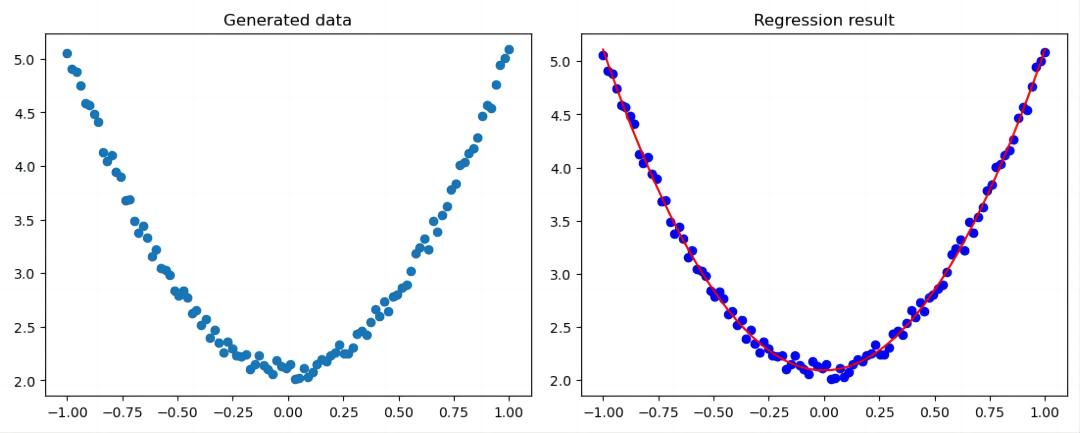
\includegraphics[width=0.8\textwidth]{part/人工智能/深度学习框架/pic/Pytorch/Pytorch基础/Numpy版实现回归问题.png}
            \caption{Numpy版实现回归问题}
            \label{fig:Numpy版实现回归问题}
    \end{figure}

    \item 使用Tensor和autograd实现
    \begin{lstlisting}[style=pythonstyle]
    # 导入所需的库
    import numpy as np
    from matplotlib import pyplot as plt

    # 生成输入数据 x 及目标数据 y
    # 设置随机种子，生成同一份数据，以便结果复现
    torch.manual_seed(985) # np.random.seed(985)
    dtype = torch.float
    # x = np.linspace(-1, 1, 100).reshape(100, 1)
    x = torch.unsqueeze(torch.linspace(-1, 1, 100), dim=1) 
    # 在第1维增加一个维度
    # 为了后面的矩阵相乘y_pred = x.pow(2).mm(w)，需要将 x 转换为矩阵形式
    #y = 3 * np.power(x, 2) + 2 + 0.2 * np.random.rand(x.size).reshape(100, 1)
    y = 3 * x.pow(2) + 2 + 0.2 * torch.rand(x.size())
    plt.title("Generated data")
    plt.scatter(x.numpy(), y.numpy()) # 画图时需要将张量转换为 numpy 数组
    plt.show()

    ################################
    # 回归模型
    # 1.初始化参数
    # w = np.random.rand(1, 1)
    w = torch.rand(1, 1, dtype=dtype, requires_grad=True)
    # b = np.random.rand(1, 1)
    b = torch.rand(1, 1, dtype=dtype, requires_grad=True)

    # 2.训练模型
    lr = 0.001  # 学习率
    epochs = 1000  # 迭代次数
    for i in range(epochs):
        # 1)前向传播
        # y_pred = np.power(x, 2).dot(w) + b
        y_pred = x.pow(2).mm(w) + b # .mm()表示矩阵相乘
        # 2)计算损失
        loss = 0.5 * (y_pred - y) ** 2
        loss = loss.sum()
        # 3)自动计算梯度
        # grad_w = np.sum((y_pred - y) * np.power(x, 2))
        # grad_b = (y_pred - y).sum()
        loss.backward()
        # 4)更新参数,使用梯度下降法使得损失函数最小
        # w -= lr * grad_w
        # b -= lr * grad_b
        with torch.no_grad(): # 不记录梯度
            w -= lr * w.grad
            b -= lr * b.grad
            # 梯度清零
            w.grad.zero_()
            b.grad.zero_()
        
        # if i % 100 == 0:
        #     print(f"Epoch {i}, Loss {loss}")
        if i % 100 == 0:
            print(f"Epoch {i}, Loss {loss.item()}")

    ################################  
    # 可视化结果
    plt.title("Regression result")
    plt.plot(x.numpy(), y_pred.detach().numpy(), 'r-', label='predict', linewidth=4) # detach() 从计算图中分离
    plt.scatter(x.numpy(), y.numpy(), color='blue', marker='o', label='true')
    plt.legend()
    plt.show()        
    \end{lstlisting}
    \begin{lstlisting}[style=demostyle,numbers=none]
    Epoch 0, Loss 431.41571044921875
    Epoch 100, Loss 2.9688427448272705
    Epoch 200, Loss 0.6887450218200684
    Epoch 300, Loss 0.2506664991378784
    Epoch 400, Loss 0.16649889945983887
    Epoch 500, Loss 0.1503276824951172
    Epoch 600, Loss 0.1472204625606537
    Epoch 700, Loss 0.14662344753742218
    Epoch 800, Loss 0.1465088278055191
    Epoch 900, Loss 0.14648674428462982
    \end{lstlisting}       
    \begin{figure}[htpb]
    \centering
    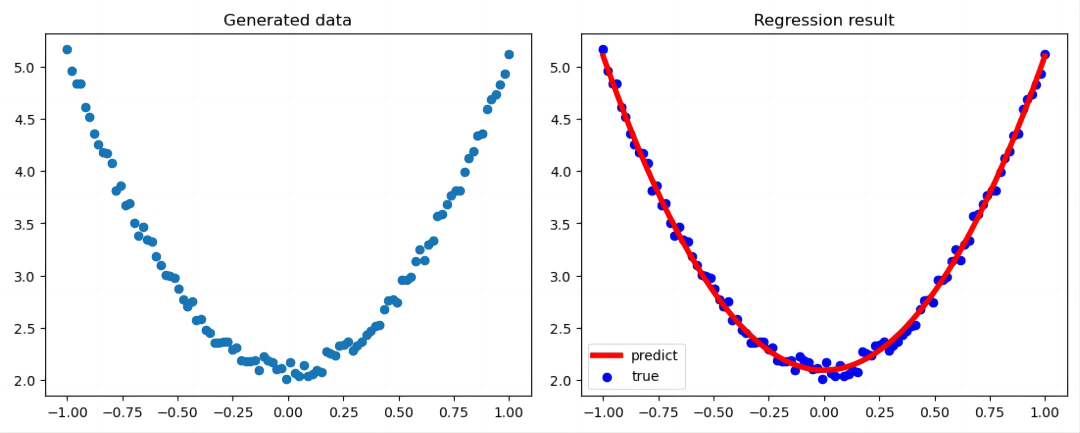
\includegraphics[width=0.8\textwidth]{part/人工智能/深度学习框架/pic/Pytorch/Pytorch基础/使用Tensor和autograd实现.png}
    \caption{使用Tensor和autograd实现}
    \label{fig:使用Tensor和autograd实现}
    \end{figure}

    如果1元2次函数使用两个参数$w_1$、$w_2$和$b$，则代码如下：
    \begin{lstlisting}[style=pythonstyle]
    # 导入所需的库
    import torch
    from matplotlib import pyplot as plt
    
    # 生成输入数据 x 及目标数据 y
    # 设置随机种子，生成同一份数据，以便结果复现
    torch.manual_seed(985)  # 设置随机种子
    
    # 使用 PyTorch 生成训练数据
    x = torch.linspace(-1, 1, 100).reshape(100, 1)  # 生成 100 个数据点
    # y = 3 * x.pow(2) + 2 + 0.2 * torch.rand(x.size())  # 生成目标数据 y
    y = 3 * x**2 + 2 + 0.2 * torch.randn(100, 1)  # 生成目标数据 y
    
    plt.title("Generated data")
    plt.scatter(x.numpy(), y.numpy())  # 画图时需要将张量转换为 numpy 数组
    plt.show()
    
    ################################
    # 回归模型
    # 1.初始化参数
    # w1 x^2 + w2 x + b
    w1 = torch.rand((1, 1), dtype=torch.float, requires_grad=True)  # 初始化权重，启用梯度
    w2 = torch.rand((1, 1), dtype=torch.float, requires_grad=True)  # 初始化权重，启用梯度
    b = torch.rand((1, 1), dtype=torch.float, requires_grad=True)  # 初始化偏置，启用梯度
    
    # 2.训练模型
    lr = 0.01  # 学习率
    epochs = 1000  # 迭代次数
    for i in range(epochs):
        # 1)前向传播
        y_pred = x.pow(2).mm(w1) + x.mm(w2) + b  # 使用 PyTorch 矩阵乘法
    
        # 2)计算损失
        loss = 0.5 * (y_pred - y).pow(2).sum()  # 使用 PyTorch 的张量操作计算损失
        # loss = (0.5 * (y_pred - y) ** 2).mean()
    
        # 3)反向传播
        loss.backward()  # 自动计算梯度
    
        # 4)更新参数,使用梯度下降法使得损失函数最小
        with torch.no_grad():
            w1 -= lr * w1.grad  # 更新权重
            w2 -= lr * w2.grad
            b -= lr * b.grad  # 更新偏置
            # 清零梯度
            w1.grad.zero_()
            w2.grad.zero_()
            b.grad.zero_()
    
        # 每100次迭代输出一次损失值
        if i % 100 == 0:
            print("epoch: {}, loss: {}".format(i, loss.item()))
            plt.scatter(x.numpy(), y.numpy())
            plt.plot(x.numpy(), y_pred.detach().numpy(), 'r-', label='predict')
            plt.title("Regression result")
            plt.legend()
            plt.show()
    
    print("w1: ", w1, "w2: ", w2, "b: ", b)
    \end{lstlisting}
    \begin{lstlisting}[style=demostyle,numbers=none]
    epoch: 0, loss: 386.6900939941406
    epoch: 100, loss: 1.4194867610931396
    epoch: 200, loss: 1.4194862842559814
    epoch: 300, loss: 1.4194862842559814
    epoch: 400, loss: 1.4194862842559814
    epoch: 500, loss: 1.4194862842559814
    epoch: 600, loss: 1.4194862842559814
    epoch: 700, loss: 1.4194862842559814
    epoch: 800, loss: 1.4194862842559814
    epoch: 900, loss: 1.4194862842559814
    w1:  tensor([[3.0083]], requires_grad=True) 
    w2:  tensor([[-0.0228]], requires_grad=True) 
    b:  tensor([[1.9803]], requires_grad=True)
    \end{lstlisting}
        
 
    \item 使用优化器及自动微分实现
    \begin{lstlisting}[style=pythonstyle]
    # 导入所需的库
    import numpy as np
    from matplotlib import pyplot as plt

    # 生成输入数据 x 及目标数据 y
    # 设置随机种子，生成同一份数据，以便结果复现
    torch.manual_seed(985) # np.random.seed(985)
    dtype = torch.float
    # x = np.linspace(-1, 1, 100).reshape(100, 1)
    x = torch.unsqueeze(torch.linspace(-1, 1, 100), dim=1) # 在第1维增加一个维度
    #y = 3 * np.power(x, 2) + 2 + 0.2 * np.random.rand(x.size).reshape(100, 1)
    y = 3 * x.pow(2) + 2 + 0.2 * torch.rand(x.size())
    plt.title("Generated data")
    plt.scatter(x.numpy(), y.numpy()) # 画图时需要将张量转换为 numpy 数组
    plt.show()

    ################################
    # 回归模型
    # 1.初始化参数
    # w = np.random.rand(1, 1)
    w = torch.rand(1, 1, dtype=dtype, requires_grad=True)
    # b = np.random.rand(1, 1)
    b = torch.rand(1, 1, dtype=dtype, requires_grad=True)

    # 2.定义损失函数和优化器
    loss_func = torch.nn.MSELoss()
    optimizer = torch.optim.SGD([w, b], lr=0.001)

    # 3.训练模型
    # lr = 0.001  # 学习率
    epochs = 1000  # 迭代次数
    for i in range(epochs):
    # 1)前向传播
    # y_pred = np.power(x, 2).dot(w) + b
    y_pred = x.pow(2).mm(w) + b # .mm()表示矩阵相乘
    loss = loss_func(y_pred, y)
    # 计算损失
    # loss = 0.5 * (y_pred - y) ** 2
    # loss = loss.sum()
    # 2)自动计算梯度
    # grad_w = np.sum((y_pred - y) * np.power(x, 2))
    # grad_b = (y_pred - y).sum()
    loss.backward()
    # 3)更新参数,使用梯度下降法使得损失函数最小
    # w -= lr * grad_w
    # b -= lr * grad_b
    # with torch.no_grad(): # 不记录梯度
    #     w -= lr * w.grad
    #     b -= lr * b.grad
    #     # 梯度清零
    #     w.grad.zero_()
    #     b.grad.zero_()
    optimizer.step()
    # 因通过autograd计算的梯度会累加到grad中，故每次循环需把梯度清零
    optimizer.zero_grad() 

    
    # if i % 100 == 0:
    #     print(f"Epoch {i}, Loss {loss}")
    if i % 100 == 0:
            print(f"Epoch {i}, Loss {loss.item()}")

    ################################  
    # 可视化结果
    plt.title("Regression result")
    plt.plot(x.numpy(), y_pred.detach().numpy(), 'r-', label='predict', linewidth=4) # detach() 从计算图中分离
    plt.scatter(x.numpy(), y.numpy(), color='blue', marker='o', label='true')
    plt.legend()
    plt.show()
    \end{lstlisting}   
    \begin{lstlisting}[style=demostyle,numbers=none] 
    Epoch 0, Loss 8.628314018249512
    Epoch 100, Loss 5.594874858856201
    Epoch 200, Loss 3.659278631210327
    Epoch 300, Loss 2.423168182373047
    Epoch 400, Loss 1.632761836051941
    Epoch 500, Loss 1.1263880729675293
    Epoch 600, Loss 0.8010491132736206
    Epoch 700, Loss 0.5911281108856201
    Epoch 800, Loss 0.4548189640045166
    Epoch 900, Loss 0.36548832058906555
    \end{lstlisting}   
    \begin{figure}[htpb]
            \centering
            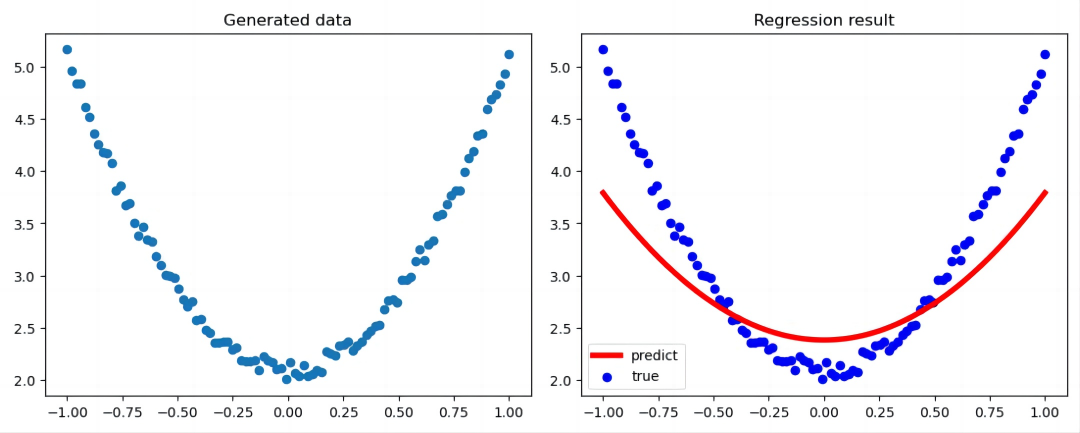
\includegraphics[width=0.8\textwidth]{part/人工智能/深度学习框架/pic/Pytorch/Pytorch基础/使用优化器及自动微分实现.png}
            \caption{使用优化器及自动微分实现}
            \label{fig:使用优化器及自动微分实现}
    \end{figure}                    

    \item 把数据集转换为带批量处理功能的迭代器
    把数据集转换为带批量处理功能的迭代器，这样训练时就可进行批量处理。
    如果数据量比较大，采用批量处理可提升训练模型的效率及性能。
    \begin{lstlisting}[style=pythonstyle]
    # 导入所需的库
    import numpy as np
    from matplotlib import pyplot as plt
    import torch

    # 生成输入数据 x 及目标数据 y
    # 设置随机种子，生成同一份数据，以便结果复现
    # np.random.seed(985)
    # x = np.linspace(-1, 1, 100).reshape(100, 1)
    # y = 3 * np.power(x, 2) + 2 + 0.2 * np.random.rand(x.size).reshape(100, 1)
    # plt.title("Generated data")
    # plt.scatter(x, y)
    # plt.show()


    ################################
    # 回归模型
    # 1.初始化参数
    # w = np.random.rand(1, 1)
    # b = np.random.rand(1, 1)
    def deta_iter(features, labels, batch_size=8):
    num_examples = len(features)
    indices = list(range(num_examples))
    # 随机读取样本，打乱顺序
    np.random.shuffle(indices)
    for i in range(0, num_examples, batch_size):
            indexs = torch.LongTensor(indices[i: min(i + batch_size, num_examples)]) # 最后一次可能不足一个batch
            yield features.index_select(0, indexs), labels.index_select(0, indexs)

    # 2.定义损失函数和优化器
    loss_func = torch.nn.MSELoss()
    optimizer = torch.optim.SGD([w, b], lr=0.001)

    # 3.训练模型
    lr = 0.001  # 学习率
    epochs = 1000  # 迭代次数
    for i in range(epochs):
    for features, labels in deta_iter(x, y, 10):
            # 1)前向传播
            y_pred = features.pow(2).mm(w) + b
            loss = loss_func(y_pred, labels)

            # 2)自动计算梯度
            loss.backward()

            # 3)更新参数,使用梯度下降法使得损失函数最小
            optimizer.step()
            optimizer.zero_grad()

    if i % 100 == 0:
            print(f"Epoch {i}, Loss {loss.item()}")
    print("w:", w, "b:", b)        

    ################################  
    # 可视化结果
    y_pred = x.pow(2).mm(w).detach().numpy() + b.detach().numpy()
    plt.title("Regression result")
    plt.plot(x.numpy(), y_pred, 'r-', label='predict', linewidth=4)
    plt.scatter(x.numpy(), y.numpy(), color='blue', marker='o', label='true')
    plt.legend()
    plt.show()
    \end{lstlisting}
    \begin{lstlisting}[style=demostyle,numbers=none]
    poch 0, Loss 0.004008688032627106
    Epoch 100, Loss 0.002615853678435087
    Epoch 200, Loss 0.002760492265224457
    Epoch 300, Loss 0.001538299024105072
    Epoch 400, Loss 0.004123619291931391
    Epoch 500, Loss 0.003147989511489868
    Epoch 600, Loss 0.0033883980941027403
    Epoch 700, Loss 0.0021358653903007507
    Epoch 800, Loss 0.004264053888618946
    Epoch 900, Loss 0.002425102051347494

    w: tensor([[3.0139]], requires_grad=True) b: tensor([[2.0920]], requires_grad=True)
    \end{lstlisting}
    \begin{figure}[htpb]
            \centering
            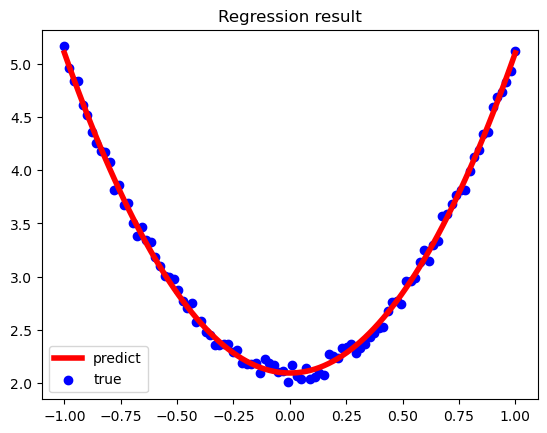
\includegraphics[width=0.8\textwidth]{part/人工智能/深度学习框架/pic/Pytorch/Pytorch基础/把数据集转换为带批量处理功能的迭代器.png}
            \caption{把数据集转换为带批量处理功能的迭代器}
            \label{fig:把数据集转换为带批量处理功能的迭代器}
    \end{figure}

\end{enumerate}


\chapter{PyTorch数据处理}
\label{cha:pytorch数据处理}

\section{数据处理工具箱概述}
\label{sec:pytorch_数据处理工具箱概述}
PyTorch提供了一系列数据处理工具箱，主要包括以下几个部分。
\begin{enumerate}[label=\arabic*)]
    \item torch.utils.data：数据加载工具箱，提供了Dataset、DataLoader等工具。
    \item torchvision：图形处理工具箱，提供了常用的数据集加载、数据预处理、图像处理等工具。
    \item torchaudio：音频处理工具箱，提供了音频数据加载、音频数据处理等工具。
    \item torchtext：文本处理工具箱，提供了文本数据加载、文本数据处理等工具。
\end{enumerate}

\section{utils.data}
\label{sec:pytorch_utils.data}
是torch.utils.data工具包，它包括以下4个类。
\begin{enumerate}[label=\arabic*)]
    \item Dataset ： 一个抽象类，其他数据集需要继承这个类，并且覆写其中的两个方法(\codeinline{\_\_getitem\_\_}、\codeinline{\_\_len\_\_})。

    \item (\textcolor{red}{\textbf{数据模块核心}})DataLoader：定义一个新的迭代器，实现批量(batch)读取，打乱数据(shuffle)并提供并行加速等功能。
    因为\codeinline{\_\_getitem\_\_}\textcolor{red}{\textbf{一次只能}}获取一个样本，
    所以通过\codeinline{torch.utils.data.DataLoader}来实现批量读取。

    \item \codeinline{random\_split}：把数据集随机拆分为给定长度的非重叠新数据集。
    \item \codeinline{*Sampler}：多种采样函数。
\end{enumerate}

dataset负责与磁盘打交道，将磁盘上的数据读取并预处理好，提供给DataLoader，
而DataLoader只需要关心如何组装成批数据，以及如何采样。
采样的体现是出现在传入getitem函数的索引，这里采样的规则可以通过sampler由用户自定义，
可以方便地实现均衡采样、随机采样、有偏采样、渐进式采样等。
\begin{figure}[htpb]
    \centering
    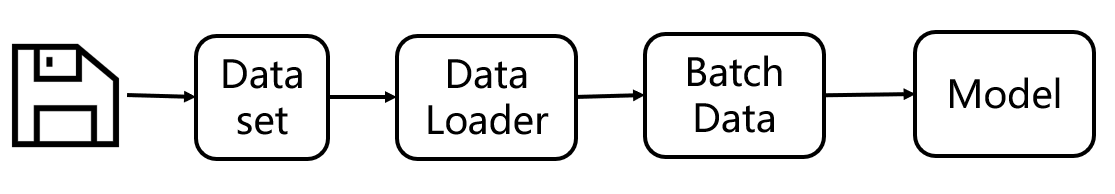
\includegraphics[width=0.6\textwidth]{part/人工智能/深度学习框架/pic/Pytorch/PyTorch数据处理/Dataset与DataLoader的关系.png}
    \caption{Dataset与DataLoader的关系}
    \label{fig:Dataset与DataLoader的关系}
\end{figure}


\subsection{Dataset 数据交互模块}
\label{subsec:pytorch_Dataset}
pytorch提供的torch.utils.data.Dataset类是一个抽象基类An abstract class representing a Dataset，供用户继承，
编写自己的dataset，实现对数据的读取。

在Dataset类的编写中\textcolor{red}{\textbf{必须}}要实现的两个函数是
\begin{enumerate}[label=\arabic*)]
    \item \codeinline{\_\_getitem\_\_}：
    通过给定索引(index)获取数据、标签或一个样本。
    然后实现从磁盘中读取数据，并进行预处理（包括online的数据增强），
    然后返回一个样本的数据。
    
    数据可以是包括模型需要的输入、标签，也可以是其他元信息，例如图片的路径。
    \codeinline{\_\_getitem\_\_}返回的数据会在dataloader中组装成一个batch。
    即，通常情况下是在dataloader中调用Dataset的\codeinline{\_\_getitem\_\_}函数获取一个样本。

    \item \codeinline{\_\_len\_\_}：返回数据集的长度。
\end{enumerate}


\begin{lstlisting}[style=pythonstyle]
# 导入需要的库
import torch
from torch.utils import data
import numpy as np

# 定义获取数据集的类
class TestDataset(data.Dataset): # 继承 Dataset，自定义数据集类
    def __init__(self):
        self.Data = np.asarray([[0, 1], [2, 3], [2, 1], [3, 4], [4, 5]])
        self.Label = np.asarray([0,1,3,5,2])

    # __getitem__方法用来获取数据集中第index个样本
    def __getitem__(self, index):
        # 把numpy转换为Tensor
        txt = torch.from_numpy(self.Data[index])
        label = torch.tensor(self.Label[index])
        return txt, label

    def __len__(self):
        return len(self.Data)

# 获取数据集中的数据
Test = TestDataset()
print(Test[2]) # 相当于调用 __getitem__(2) 方法
print(Test.__getitem__(2))
print(Test.__len__()) 
print(Test[0]) # 相当于调用 __getitem__(0) 方法
\end{lstlisting}
\begin{lstlisting}[style=demostyle,numbers=none] 
(tensor([2, 1]), tensor(3))
(tensor([2, 1]), tensor(3))  # 两者等价
5
(tensor([0, 1]), tensor(0))
\end{lstlisting}    

以上数据以元组格式返回，每次只返回一个样本。

\subsection{DataLoader 数据加载模块}
\label{subsec:pytorch_DataLoader}
实际上，Dataset只负责数据的抽取，一次调用\codeinline{\_\_getitem\_\_}只返回一个样本。
如果希望批量处理，同时进行数据打乱和并行加速等操作，
可选择\codeinline{DataLoader}。DataLoader的格式为：
\begin{lstlisting}[style=demostyle,numbers=none] 
data.DataLoader(
    dataset,        # 数据集
    batch_size=1,   # 批量大小
    shuffle=False,  # 是否打乱数据
    sampler=None,   # 样本抽样
    batch_sampler=None,  # 批量抽样
    num_workers=0,  # 并行线程数,0代表不使用多进程
    collate_fn=None,    # ：如何将多个样本数据拼接成一个批量，一般使用默认的拼接方式即可
    pin_memory=False,   # 是否将数据保存在锁页内存(pin_memory)区，
                        # pin_memory中的数据转到GPU会快一些。    
    drop_last=False,    # 是否丢弃最后一个不完整的 batch
                        # dataset中的数据个数可能不是batch_size的整数倍，
                        # 将drop_last设置为True时会将多出来且不足一个批量的数据丢弃。
    timeout=0,          # 加载数据超时时间
    worker_init_fn=None,    # 每个 worker 初始化函数
    multiprocessing_context=None,  # 多进程上下文
    generator=None, *, # 生成器
    prefetch_factor=2,  # 预取因子
    persistent_workers=False # 是否使用持久化工作进程
)   
\end{lstlisting} 

\begin{lstlisting}[style=pythonstyle]
# 导入需要的库
import torch
from torch.utils import data
import numpy as np

# 定义获取数据集的类
class TestDataset(data.Dataset): # 继承 Dataset，自定义数据集类
    def __init__(self):
        self.Data = np.asarray([[0, 1], [2, 3], [2, 1], [3, 4], [4, 5]])
        self.Label = np.asarray([0, 1, 0, 1, 2])

    def __getitem__(self, index):
        # 把numpy转换为Tensor
        txt = torch.from_numpy(self.Data[index])
        label = torch.tensor(self.Label[index])
        return txt, label

    def __len__(self):
        return len(self.Data)

# 获取数据集中的数据
Test = TestDataset()
#####################
# 1)单个获取
# print(Test[2]) # 相当于调用 __getitem__(2) 方法
# print(Test.__len__()) # 相当于调用 __len__() 方法    
# print(Test[0]) # 相当于调用 __getitem__(0) 方法

#####################
# 2)使用DataLoader加载数据
test_loader = data.DataLoader(Test, batch_size=3, shuffle=False, num_workers=2)
for i, data in enumerate(test_loader):
    inputs, labels = data
    print(f"Batch {i}:")
    print(f"数据：{inputs}")
    print(f"标签：{labels}\n")

print("-------------------------")
# 批量读取。我们可以像使用迭代器一样使用它，如对它进行循环操作。不过它不是迭代器，可以通过iter命令转换为迭代器。    
dataiter = iter(test_loader)
inputs, labels = next(dataiter)
print(f"数据：{inputs}")
print(f"标签：{labels}")
\end{lstlisting}

批量读取我们可以像使用迭代器一样使用它，如对它进行循环操作。
不过它不是迭代器，可以通过\codeinline{iter}命令转换为迭代器。

\begin{lstlisting}[style=demostyle,numbers=none] 
Batch 0:
数据：tensor([[0, 1],
        [2, 3],
        [2, 1]])
标签：tensor([0, 1, 0])

Batch 1:
数据：tensor([[3, 4],
        [4, 5]])
标签：tensor([1, 2])

-------------------------
数据：tensor([[0, 1],
        [2, 3],
        [2, 1]])
标签：tensor([0, 1, 0])
\end{lstlisting}

    
    

\section{torchvision 图形处理工具箱}
\label{sec:pytorch_torchvision}
torchvision包括4个类，各类的主要功能如下。
\begin{enumerate}[label=\arabic*)]
    \item datasets：提供常用的数据集加载，设计上都是继承\codeinline{torch.utils.data.Dataset},主要包括MNIST、CIFAR10/100. ImageNet. COCO 等。
    \item models：提供深度学习中各种经典的网络结构以及训练好的模型（如果要选择训练好的模型，则设置\codeinline{pretrained = True})，包括AlexNet、VGG系列、ResNet系列Inception系列等。
    \item transforms：常用的数据预处理操作，主要包括对\codeinline{Tensoi}及\codeinline{PIL Image}对象的操作。
    \item utils：含两个函数，一个是\codeinline{make\_grid},它能将多张图像拼接在一个网格中；另一个是\codeinline{savejmg},它能将\codeinline{Tensor}保存为图像。
\end{enumerate}

\subsection{torchvision安装}
\label{subsec:pytorch_torchvision安装}
torchvision是PyTorch的一个视觉处理工具包，独立于PyTorch,需要另外安装。
\begin{lstlisting}[style=demostyle,numbers=none] 
pip install torchvision
# 或者
conda install torchvision
\end{lstlisting}

\subsection{torchvision.datasets}
\label{subsec:pytorch_torchvision.datasets}

\subsection{torchvision.models}
\label{subsec:pytorch_torchvision.models}

\subsection{torchvision.transforms}
\label{subsec:pytorch_torchvision.transforms}
transforms提供了对PIL Image对象和Tensor对象的常用操作。

对 PIL Image 的操作包括：
\begin{enumerate}[label=\arabic*)]
    \item \codeinline{Scale/Resize}：调整图片尺寸，长宽比保持不变。
    \item \codeinline{CenterCrop}：从中心开始裁剪图片。
    \item \codeinline{RandomCrop}：随机裁剪。
    \item \codeinline{RandomSizeCrop}：随机尺寸裁剪。
    \item \codeinline{Pad}:填充。
    \item \codeinline{ToTensor}：将PIL Image对象转为Tensor，
    会自动将[0,255]归一化至[0,1]。
    \item \codeinline{RandomHorizontalFlip}：随机水平翻转,概率为0.5。
    \item \codeinline{RandomVerticalFlip}：随机垂直翻转,概率为0.5。
    \item \codeinline{ColorJitter}：调整亮度、对比度、饱和度和色相。
\end{enumerate}

对 Tensor 的操作包括：
\begin{enumerate}[label=\arabic*)]
    \item \codeinline{Normalize}：标准化。
    \item \codeinline{ToPILImage}：将Tensor转为PIL Image对象。
\end{enumerate}

如果要对数据集进行多个操作，可通过Compose将这些操作像管道一样拼接起来，
类似于\codeinline{nn.Sequential}

\begin{lstlisting}[style=demostyle,numbers=none] 
# 例如    
transforms.Compose([
    # 从图片中间裁剪出224*224的图片
    transforms.RandomResizedCrop(224),
    # 随机水平翻转，概率为0.5
    transforms.RandomHorizontalFlip(),
    # 将图片像素值归一化
    transforms.ToTensor(),
    # 标准化
    transforms.Normalize(mean=[0.485, 0.456, 0.406],
                         std=[0.229, 0.224, 0.225])
])
\end{lstlisting}    



\subsection{torchvision.utils}
\label{subsec:pytorch_torchvision.utils}









\section{可视化工具}
\label{sec:pytorch_可视化工具}
\subsection{TensorBoard}
\label{subsec:pytorch_tensorboard}
TensorBoard是Google TensorFlow的可视化工具，
可以记录训练数据、评估数据、网络结构、图像等，
并且可以在Web上展示，对于观察神经网络训练的过程非常有帮助。
PyTorch支持\codeinline{tensorboard\_logger}、\codeinline{visdom}等可视化工具。

TensorBoard 功能很强大，支持 scalar、image、figureA histogram、audio、text、
graph、onnx\_graph、embedding、 pr\_curve、videosummaries 等可视化方式。 

\subsubsection{安装}
\label{subsubsec:pytorch_tensorboard安装}
\begin{lstlisting}[style=demostyle,numbers=none] 
pip install tensorboard
\end{lstlisting}

\subsubsection{使用}
\label{subsubsec:pytorch_tensorboard使用}

执行下面命令
\begin{lstlisting}[style=demostyle,numbers=none] 
tensorboard --logdir=<event文件目录>
\end{lstlisting}

复制网址\url{http://localhost:6006/} 到浏览器中进行打开

\begin{enumerate}[label=\arabic*)]
    \item 如果conda环境下没有安装tensorboard，可以通过以下命令启动tensorboard。
    \begin{lstlisting}[style=demostyle,numbers=none] 
    tensorboard --logdir=/home/tony/Pratice/Python/Pytorch/NFEM --port 6006 --load_fast=false
    \end{lstlisting}

    \item 在tensorboard启动的过程中，可能发生的问题：

    6006端口被占用：
    \begin{lstlisting}[style=demostyle,numbers=none] 
    port 6006 was already in use 
    E0117 15:58:38.631224 MainThread program.py:260] TensorBoard attempted to bind to port 6006, but it was already in use
    TensorBoard attempted to bind to port 6006, but it was already in use
    \end{lstlisting}
    
    解决方法：修改端口为6007
    \begin{lstlisting}[style=demostyle,numbers=none] 
    tensorboard --logdir=your_dir --port=6007
    \end{lstlisting}
\end{enumerate}

\begin{lstlisting}[style=pythonstyle]
# 可视化神经网络  
# 导入需要的模块。  
import torch  
import torch.nn as nn  
import torch.nn.functional as F  
import torchvision  
from torch.utils.tensorboard import SummaryWriter  

import os
log_dir = os.getcwd()  # 或者指定一个相对于当前工作目录的子目录，如 'logs'  

# 1.构建神经网络。  
class Net(nn.Module):  
    def __init__(self):  
        super(Net, self).__init__()  
        self.conv1 = nn.Conv2d(1, 10, kernel_size=5)  
        self.conv2 = nn.Conv2d(10, 20, kernel_size=5)  
        self.conv2_drop = nn.Dropout2d()  
        self.fc1 = nn.Linear(320, 50)  
        self.fc2 = nn.Linear(50, 10)  
        self.bn = nn.BatchNorm2d(20)  
  
    def forward(self, x):  
        x = F.max_pool2d(self.conv1(x), 2)  
        x = F.relu(x) + F.relu(-x)  # 这里是双边ReLU，通常不常见，可能是个实验性设计  
        x = F.relu(F.max_pool2d(self.conv2_drop(self.conv2(x)), 2))  
        x = self.bn(x)  
        x = x.view(-1, 320)  
        x = F.relu(self.fc1(x))  
        x = F.dropout(x, training=self.training)  
        x = self.fc2(x)  
        x = F.softmax(x, dim=1)  
        return x  
  
# 2.把模型保存为图像  
# 1）定义输入。          
input_tensor = torch.rand(1, 1, 28, 28)  
# 2）实例化模型。  
model = Net()  
# 3）把模型保存为图像。  
with SummaryWriter(log_dir=log_dir, comment='Net') as w:  
    w.add_graph(model, (input_tensor, ))
\end{lstlisting}
\begin{lstlisting}[style=pythonstyle]
# 可视化损失函数
# 可视化损失值时需要用到add_scalar函数，这里利用一层全连接神经网络，训练一元二次函数的参数。
import torch
import torch.nn as nn
from torch.utils.tensorboard import SummaryWriter
import numpy as np

input_size = 1
output_size = 1
num_epoches = 60
learning_rate = 0.01

dtype = torch.FloatTensor
writer = SummaryWriter(log_dir='logs',comment='Linear')
np.random.seed(100) 
x_train = np.linspace(-1, 1, 100).reshape(100,1) 
y_train = 3*np.power(x_train, 2) +2+ 0.2*np.random.rand(x_train.size).reshape(100,1) 

model = nn.Linear(input_size, output_size)

criterion = nn.MSELoss()
optimizer = torch.optim.SGD(model.parameters(), lr=learning_rate)

for epoch in range(num_epoches):
    inputs = torch.from_numpy(x_train).type(dtype)
    targets = torch.from_numpy(y_train).type(dtype)

    output = model(inputs)
    loss = criterion(output, targets)

    optimizer.zero_grad()
    loss.backward()
    optimizer.step()
    # 保存loss的数据与epoch数值
    writer.add_scalar('训练损失值', loss, epoch)
\end{lstlisting}



\chapter{PyTorch神经网络工具}
\label{chap:pytorch_nn_tools}
利用这个工具箱设计一个神经网络就像搭积木一样，可以极大简化构建模型的任务。

\section{神经网络核心组件}
\label{sec:Pytorch_nn_core_components}
神经网络核心部分或组件不多，我们确定这些组件后，这个就基本确定了神经网络。
这些核心组件分析如下
\begin{enumerate}[label=\arabic*)]
    \item 层：神经网络的基本结构，将输入张量转换为输出张量。 
    \item 模型：由层构成的网络。 
    \item 损失函数：参数学习的目标函数，通过最小化损失函数来学习各种参数。 
    \item 优化器：如在使损失值最小时，就会涉及优化器。 
\end{enumerate}

\begin{figure}[htpb]
    \centering
    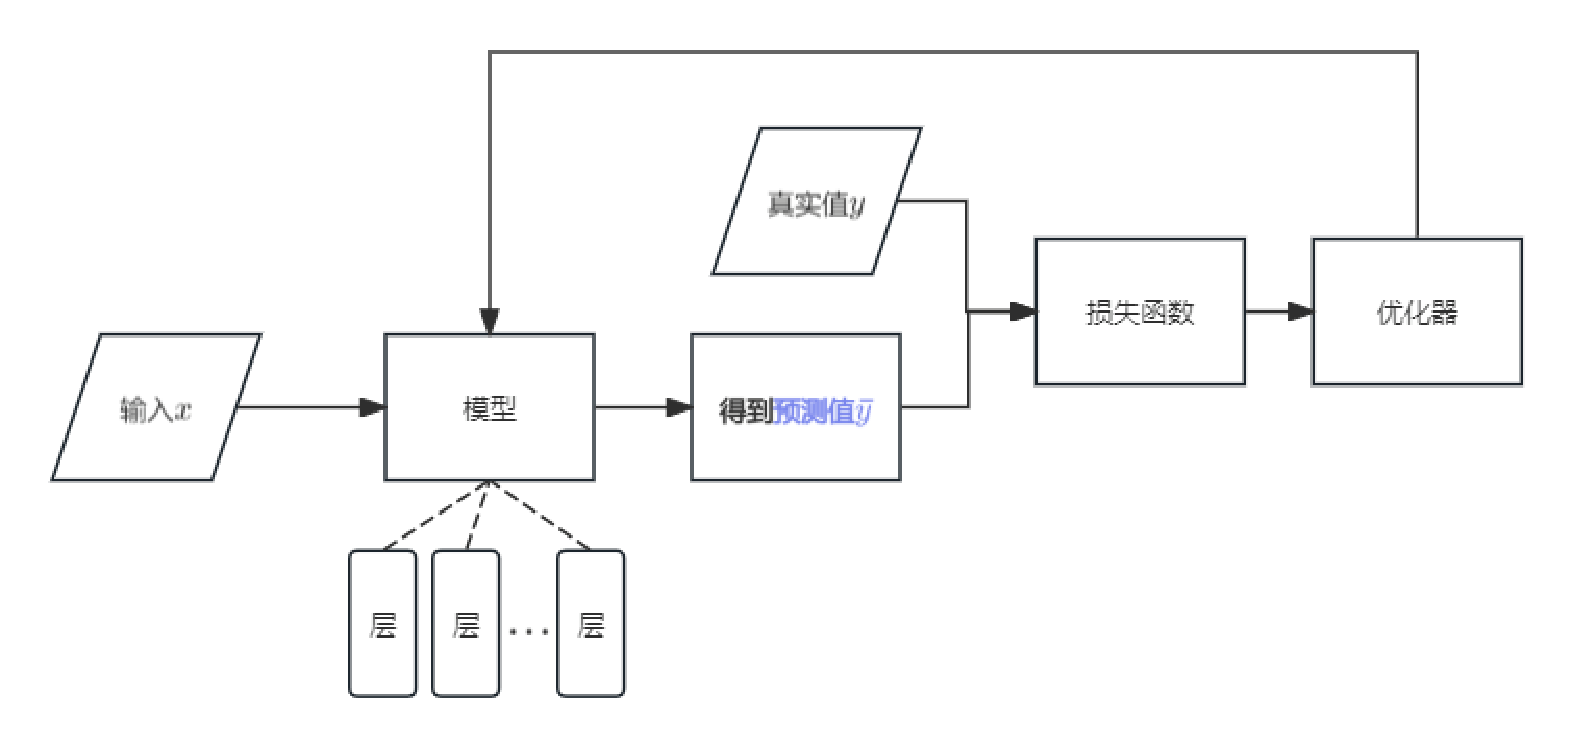
\includegraphics[width=0.8\textwidth]{part/人工智能/深度学习框架/pic/Pytorch/PyTorch神经网络工具/神经网络关键组件及相互关系示意图.pdf}
    \caption{神经网络关键组件及相互关系示意图}
    \label{fig:Pytorch_nn_core_components}
\end{figure}

如图\ref{fig:Pytorch_nn_core_components}所示，
多个层链接在一起构成一个模型或网络，输入数据通过这个模型转换为预测值。
预测值与真实值共同构成损失函数的输入，损失函数输出损失值（损失值可以是距离、概率值等），
该损失值用于衡量预测值与目标结果的匹配或相似程度。
优化器利用损失值更新权重参数，目标是使损失值越来越小。
这是一个循环过程，当损失值达到一个阈值或循环次数到达指定次数时，循环结束。


\section{构建神经网络的主要工具}
\subsection{nn.Module}
使用autograd及Tensor实现机器学习实例时，需要做不少设置，
如将叶子节点的参数\codeinline{requires\_grad}设置为\codeinline{True},
然后调用\codeinline{backward}函数从grad属性中提取梯度。
对于大规模的网络，autograd太过于底层和烦琐。
为了简单、有效地解决这个问题，\codeinline{nn}是一个有效工具。 
它是专门为深度学习设计的一个模块，而\codeinline{nn.Module}是\codeinline{nn}的一个核心数据结构。
\codeinline{nn.Module}可以是神经网络的某个层，也可以是包含多层的神经网络。
在实际使用中，最常见的做法是继承\codeinline{nn.Module}生成自己的网络层，

\codeinline{nn.Module}是PyTorch中所有神经网络模块的基类，
所有神经网络模块都应该继承自\codeinline{nn.Module}。

\subsection{nn.functional}
\label{subsubsec:Pytorch_nn_functional}
\codeinline{nn.functional}是一个函数模块，包含了神经网络中的一些常用函数，
如激活函数、损失函数、池化函数等。


\subsubsection{nn.Module和nn.functional的区别}
\label{subsubsec:Pytorch_nn_Module_and_nn_functional_difference}
\codeinline{nn}中的层，
\begin{enumerate}[label=\arabic*)]
    \item 继承了 \codeinline{nn.Module}，名称一般为\codeinline{nn.Xxx}(第一个是大写)

    如\codeinline{nn.Linear}、\codeinline{nn.Conv2d}、\codeinline{nn.CrossEntropyLoss} 等。

    \item  \codeinline{nn.functional} 中的函数，名称一般为 \codeinline{nn.functional.xxx}(第一个是小写)，

    如\codeinline{nn.functional.linear}、\codeinline{nn.functional.conv2d}、
 \codeinline{nn.functional.cross\_entropy} 等。
\end{enumerate}
 
  
从功能方面来说两者相当，基于\codeinline{nn.Module}实现的层，也可以基于\codeinline{nn.functional} 实现，反之亦然。
从性能方面来说两者也没有太大差异。不过在具体使用时，两者还是有区别的

\begin{enumerate}[label=\arabic*)]
    \item \codeinline{nn.Xxx}继承于\codeinline{nn.Module},需要先实例化并传入参数，
    然后以函数调用的方式调用实例化的对象并传入输入数据。它能够很好地与\codeinline{nn.Sequential}结合使用

    而\codeinline{nn.functional.xxx}是一个函数。它无法保存参数，因此无法使用\codeinline{nn.Sequential}。
    \item \codeinline{nn.Xxx}中的层可以\textcolor{YBXPurple}{自动}定义、保存参数，如\codeinline{nn.Linear}中的权重和偏置，

    而\codeinline{nn.functional.xxx}中的函数不具备保存参数的功能，不仅需要自己定义参数(权重(weights)和偏置(bias)等)，还需要手动传入参数。

    \item \codeinline{dropout}操作在训练和测试阶段是不同的，
    使用\codeinline{nn.Xxx}方式定义的\codeinline{dropout}层，在调用\codeinline{model.eval()}后，自动实现状态的转换，

    而使用\codeinline{nn.functional.xxx}方式定义的\codeinline{dropout}函数，需要手动设置状态。
\end{enumerate}

总的来说，两种函数的功能都是相同的，但PyTorch官方推荐：
\begin{enumerate}[label=\arabic*)]
    \item 具有学习参数的
    （例如，conv2d、linear、batchjnorm、dropout等）情况采用\codeinline{nn.Xxx}方式，
    \item 没有学习参数的
    （例如， maxpool, loss func, activation fimc 等）情况采用 \codeinline{nn.functional.xxx} 或者 \codeinline{nn.Xxx} 方式。
\end{enumerate}

\begin{lstlisting}[style=pythonstyle]
# 使用 nn.Module 定义一个简单的神经网络    
import torch
import torch.nn as nn
import torch.optim as optim

# 定义一个简单的神经网络，继承自 nn.Module
class Net(nn.Module):
    def __init__(self):
        super(Net, self).__init__()
        # 使用 nn.Xxx 自动定义和保存参数
        self.fc1 = nn.Linear(10, 20)
        self.fc2 = nn.Linear(20, 10)
        self.dropout = nn.Dropout(p=0.5)  # 定义 Dropout 层

    def forward(self, x):
        x = self.fc1(x)
        x = self.dropout(x)
        x = self.fc2(x)
        return x

# 使用 nn.Sequential 结合多层
net = nn.Sequential(
    nn.Linear(10, 20),
    nn.ReLU(),
    nn.Dropout(p=0.5),
    nn.Linear(20, 10)
)

# 打印 Dropout 在训练模式下的状态
print("Training mode:")
print(net)

# 创建一个随机输入张量
input_data = torch.randn(5, 10)

# 模型实例化并调用
model = Net()
output = model(input_data)

# 切换到 eval 模式，Dropout 状态将自动切换
print("Dropout before eval:", model.dropout.training)
model.eval()
print("Eval mode:")
print(model)

# 在训练和测试模式下输出模型的 Dropout 状况
model.eval()  # 切换到评估模式
print("Dropout after eval:", model.dropout.training)

# 训练优化器设置
optimizer = optim.SGD(model.parameters(), lr=0.01)
\end{lstlisting}
\begin{lstlisting}[style=demostyle,numbers=none] 
Training mode:
Sequential(
  (0): Linear(in_features=10, out_features=20, bias=True)
  (1): ReLU()
  (2): Dropout(p=0.5, inplace=False)
  (3): Linear(in_features=20, out_features=10, bias=True)
)
Dropout before eval: True
Eval mode:
Net(
  (fc1): Linear(in_features=10, out_features=20, bias=True)
  (fc2): Linear(in_features=20, out_features=10, bias=True)
  (dropout): Dropout(p=0.5, inplace=False)
)
Dropout after eval: False    
\end{lstlisting}
\begin{lstlisting}[style=pythonstyle]
# 使用 nn.functional 定义一个简单的神经网络
import torch
import torch.nn.functional as F

# 自定义一个简单的神经网络，不继承 nn.Module
class FunctionalNet:
    def __init__(self):
        # 手动定义权重和偏置
        self.weight1 = torch.randn(20, 10, requires_grad=True)
        self.bias1 = torch.randn(20, requires_grad=True)
        self.weight2 = torch.randn(10, 20, requires_grad=True)
        self.bias2 = torch.randn(10, requires_grad=True)
        self.dropout_p = 0.5
        self.training = True

    def forward(self, x):
        x = F.linear(x, self.weight1, self.bias1)
        if self.training:  # 手动设置 dropout 状态
            x = F.dropout(x, p=self.dropout_p)
        x = F.linear(x, self.weight2, self.bias2)
        return x

    def eval(self):
        self.training = False  # 手动切换为评估模式

# 实例化模型并传入输入数据
model = FunctionalNet()
input_data = torch.randn(5, 10)

# 模型训练模式下
print("Training mode")
output = model.forward(input_data)

# 手动切换到评估模式，关闭 dropout
print("Dropout before eval:", model.training)
model.eval()
print("Eval mode")
print("Dropout after eval:", model.training)
output = model.forward(input_data)

# 手动更新权重（这里只是为了演示，通常在训练步骤中会通过优化器更新）
optimizer = optim.SGD([model.weight1, model.bias1, model.weight2, model.bias2], lr=0.01)
\end{lstlisting}
\begin{lstlisting}[style=demostyle,numbers=none] 
Training mode
Dropout before eval: True
Eval mode
Dropout after eval: False
\end{lstlisting}    


\section{构建模型的方法}
\label{subsec:Pytorch_build_model}
使用PyTorch构建模型的方法大致有以下3种。
\begin{enumerate}[label=\arabic*)]
    \item 继承\codeinline{nn.Module}基类构建模型。
    \item 使用\codeinline{nn.Sequential}按层顺序构建模型。
    \item 继承\codeinline{nn.Module}基类构建模型，再使用相关模型容器（如\codeinline{nn.Sequential}、\codeinline{nn.ModuleList}、\codeinline{nn.ModuleDict}等）进行封装。
\end{enumerate}

\begin{example}
    \exProblem
    如图\ref{fig:Pytorch_build_model_example}所示，使用PyTorch构建一个简单的神经网络模型，使用3种方法构建模型。
    \begin{figure}[htpb]
        \centering
        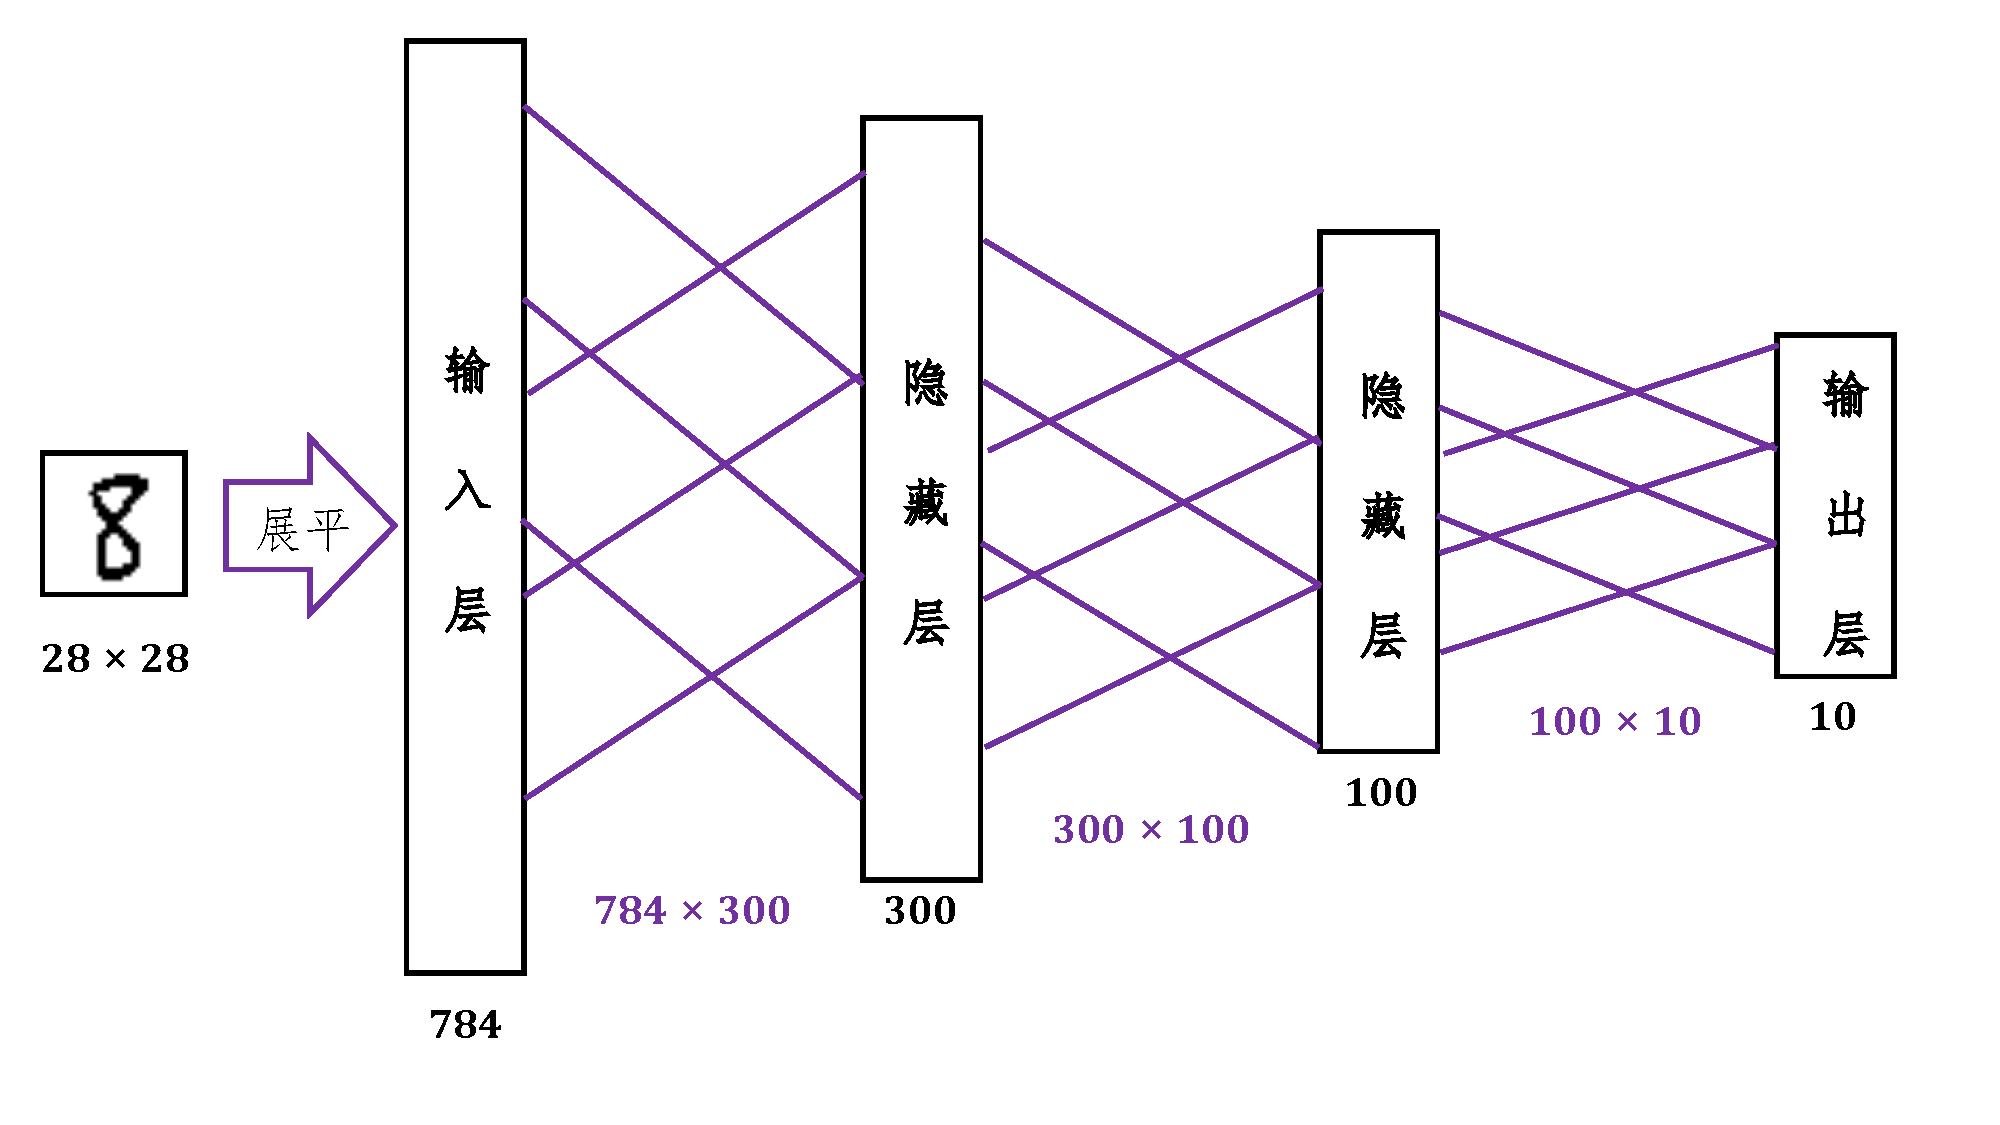
\includegraphics[width=0.8\textwidth]{part/人工智能/深度学习框架/pic/Pytorch/PyTorch神经网络工具/使用PyTorch构建模型的演示.pdf}
        \caption{使用PyTorch构建模型的演示}
        \label{fig:Pytorch_build_model_example}
    \end{figure}
    
\end{example}


\subsection{继承nn.Module基类构建模型}
\label{subsubsec:Pytorch_build_model_inherit_nn_Module}
利用这种方法构建模型，先定义一个类，使之继承\codeinline{nn.Module}基类。
把模型中需要用到的层放在构造函数\codeinline{\_\_init\_\_()}中，
在\codeinline{forward}方法中实现模型的正向传播。

\begin{lstlisting}[style=pythonstyle]
# 构建神经网络 
# 方法1.继承 nn.Module 类
import torch
from torch import nn # 导入nn 模块
import torch.nn.functional as F # 导入函数模块

###########################
class Model(nn.Module):
    def __init__(self, in_dim, n_hidden_1, n_hidden_2, out_dim):
        super(Model, self).__init__()
        self.layer1 = nn.Linear(in_dim, n_hidden_1)
        self.layer2 = nn.Linear(n_hidden_1, n_hidden_2)
        self.layer3 = nn.Linear(n_hidden_2, out_dim)

    def forward(self, x):
        x = F.relu(self.layer1(x))
        x = F.relu(self.layer2(x))
        x = self.layer3(x)
        return x
    
## 实例化模型
model = Model(10, 20, 10, 6) # 输入是10，输出是6
print(model)

x = torch.randn(10) # 这里是10
print("x:", x)
print(model.forward(x))
\end{lstlisting}
\begin{lstlisting}[style=demostyle,numbers=none] 
Model(
  (layer1): Linear(in_features=10, out_features=20, bias=True)
  (layer2): Linear(in_features=20, out_features=10, bias=True)
  (layer3): Linear(in_features=10, out_features=6, bias=True)
)
x: tensor([-1.0035,  0.4780,  0.8982,  0.0782, -1.2985, -0.5568,  0.2565,  1.2554,
         0.1004,  0.4208])
tensor([-0.0519,  0.0176,  0.0493, -0.2996, -0.1996,  0.1357], # 输出层是6个神经元
       grad_fn=<ViewBackward0>)
\end{lstlisting}

\begin{lstlisting}[style=pythonstyle]
# 导入模块
import torch
from torch import nn            # 导入 nn 模块
import torch.nn.functional as F # 导入函数模块

################################
# 构建模型
class Model_inh_mod(nn.Module): # 通过继承 nn.Module 来构建模型
    def __init__(self, in_dim, n_hidden_1, n_hidden_2, out_dim):
        super(Model_use_Seq, self).__init__()
        self.flatten = nn.Flatten() # 展平操作
        self.linear1 = nn.Linear(in_dim, n_hidden_1)
        self.bn1 = nn.BatchNorm1d(n_hidden_1) # 批量归一化
        self.linear2 = nn.Linear(n_hidden_1, n_hidden_2)
        self.bn2 = nn.BatchNorm1d(n_hidden_2)
        self.out = nn.Linear(n_hidden_2, out_dim)

    def forward(self, x):
        x = self.flatten(x)
        x = self.linear1(x)
        x = self.bn1(x)
        x = F.relu(x)
        x = self.linear2(x)
        x = self.bn2(x)
        x = F.relu(x)
        x = self.out(x)
        x = F.softmax(x, dim=1)
        return x

# 查看模型    
# 定义一个28*28的输入，
# 第一个隐藏层300个神经元，第二个隐藏层100个神经元，
# 输出层10个神经元
in_dim, n_hidden_1, n_hidden_2, out_dim = 28*28, 300, 100, 10
model = Model_inh_mod(in_dim, n_hidden_1, n_hidden_2, out_dim)
print(model)
\end{lstlisting}
\begin{lstlisting}[style=demostyle,numbers=none]
Model_inh_mod(
  (flatten): Flatten(start_dim=1, end_dim=-1)
  (linear1): Linear(in_features=784, out_features=300, bias=True)
  (bn1): BatchNorm1d(300, eps=1e-05, momentum=0.1, affine=True, track_running_stats=True)
  (linear2): Linear(in_features=300, out_features=100, bias=True)
  (bn2): BatchNorm1d(100, eps=1e-05, momentum=0.1, affine=True, track_running_stats=True)
  (out): Linear(in_features=100, out_features=10, bias=True)
)    
\end{lstlisting}


\subsection{使用nn.Sequential按层顺序构建模型}
\label{subsubsec:Pytorch_build_model_with_nn_Sequential}
\begin{enumerate}[label=\arabic*)]
    \item 利用可变参数
    Python中的函数的参数个数是可变(或称为不定长参数)的，
    PyTorch中的有些函数也与此类似，\codeinline{nn.Sequential(*args)}。
    \begin{lstlisting}[style=pythonstyle]
    # 方法2 使用nn.Sequential
    import torch
    from torch import nn

    # 定义模型
    in_dim, n_hidden_1, n_hidden_2, out_dim = 10, 20, 10, 6

    model = nn.Sequential(
        nn.Linear(in_dim, n_hidden_1),
        nn.ReLU(),
        nn.Linear(n_hidden_1, n_hidden_2),
        nn.ReLU(),
        nn.Linear(n_hidden_2, out_dim)
    )

    # 打印模型
    print(model)

    # 测试模型
    x = torch.tensor([1, 2, 3, 4, 5, 6, 7, 8, 9, 10], dtype=torch.float32)
    print("x:", x)
    print(model(x))
    \end{lstlisting}

\begin{lstlisting}[style=pythonstyle]
# 导入模块
import torch
from torch import nn            # 导入 nn 模块
# 初始化参数
in_dim, n_hidden_1, n_hidden_2, out_dim = 28*28, 300, 100, 10

################################
# 构建模型
Model_use_Seq = nn.Sequential(
    nn.Flatten(), # 展平操作
    nn.Linear(in_dim, n_hidden_1),
    nn.BatchNorm1d(n_hidden_1), # 批量归一化
    nn.ReLU(),
    nn.Linear(n_hidden_1, n_hidden_2),
    nn.BatchNorm1d(n_hidden_2),
    nn.ReLU(),
    nn.Linear(n_hidden_2, out_dim),
    nn.Softmax(dim=1)
    )

# 查看模型
model = Model_use_Seq
print(model)
\end{lstlisting}
\begin{lstlisting}[style=demostyle,numbers=none]
Sequential(
  (0): Flatten(start_dim=1, end_dim=-1)
  (1): Linear(in_features=784, out_features=300, bias=True)
  (2): BatchNorm1d(300, eps=1e-05, momentum=0.1, affine=True, track_running_stats=True)
  (3): ReLU()
  (4): Linear(in_features=300, out_features=100, bias=True)
  (5): BatchNorm1d(100, eps=1e-05, momentum=0.1, affine=True, track_running_stats=True)
  (6): ReLU()
  (7): Linear(in_features=100, out_features=10, bias=True)
  (8): Softmax(dim=1)
)
\end{lstlisting}   
    
    \item 使用\codeinline{add\_module}方法
\begin{lstlisting}[style=pythonstyle]
# 导入模块
import torch
from torch import nn            # 导入 nn 模块
# 初始化参数
in_dim, n_hidden_1, n_hidden_2, out_dim = 28*28, 300, 100, 10

################################
# 构建模型
Seq_model = nn.Sequential()
Seq_model.add_module('flatten', nn.Flatten())
Seq_model.add_module('linear1', nn.Linear(in_dim, n_hidden_1))
Seq_model.add_module('bn1', nn.BatchNorm1d(n_hidden_1))
Seq_model.add_module('relu1', nn.ReLU())
Seq_model.add_module('linear2', nn.Linear(n_hidden_1, n_hidden_2))
Seq_model.add_module('bn2', nn.BatchNorm1d(n_hidden_2))
Seq_model.add_module('relu2', nn.ReLU())
Seq_model.add_module('out', nn.Linear(n_hidden_2, out_dim))
Seq_model.add_module('softmax', nn.Softmax(dim=1))

# 查看模型
model = Seq_model
print(model)
\end{lstlisting}
\begin{lstlisting}[style=demostyle,numbers=none]
Sequential(
  (flatten): Flatten(start_dim=1, end_dim=-1)
  (linear1): Linear(in_features=784, out_features=300, bias=True)
  (bn1): BatchNorm1d(300, eps=1e-05, momentum=0.1, affine=True, track_running_stats=True)
  (relu1): ReLU()
  (linear2): Linear(in_features=300, out_features=100, bias=True)
  (bn2): BatchNorm1d(100, eps=1e-05, momentum=0.1, affine=True, track_running_stats=True)
  (relu2): ReLU()
  (out): Linear(in_features=100, out_features=10, bias=True)
  (softmax): Softmax(dim=1)
)
\end{lstlisting}

    \item 使用\codeinline{OrderedDict}方法
\begin{lstlisting}[style=pythonstyle]
# 导入模块
import torch
from torch import nn            # 导入 nn 模块
from collections import OrderedDict

# 初始化参数
in_dim, n_hidden_1, n_hidden_2, out_dim = 28*28, 300, 100, 10

################################
# 构建模型
Seq_model = nn.Sequential(OrderedDict([
    ('flatten', nn.Flatten()),
    ('linear1', nn.Linear(in_dim, n_hidden_1)),
    ('bn1', nn.BatchNorm1d(n_hidden_1)),
    ('relu1', nn.ReLU()),
    ('linear2', nn.Linear(n_hidden_1, n_hidden_2)),
    ('bn2', nn.BatchNorm1d(n_hidden_2)),
    ('relu2', nn.ReLU()),
    ('out', nn.Linear(n_hidden_2, out_dim)),
    ('softmax', nn.Softmax(dim=1))
    ]))

# 查看模型
model = Seq_model
print(model)    
\end{lstlisting}
\begin{lstlisting}[style=demostyle,numbers=none]
Sequential(
  (flatten): Flatten(start_dim=1, end_dim=-1)
  (linear1): Linear(in_features=784, out_features=300, bias=True)
  (bn1): BatchNorm1d(300, eps=1e-05, momentum=0.1, affine=True, track_running_stats=True)
  (relu1): ReLU()
  (linear2): Linear(in_features=300, out_features=100, bias=True)
  (bn2): BatchNorm1d(100, eps=1e-05, momentum=0.1, affine=True, track_running_stats=True)
  (relu2): ReLU()
  (out): Linear(in_features=100, out_features=10, bias=True)
  (softmax): Softmax(dim=1)
)
\end{lstlisting}    


\end{enumerate}

\subsection{继承nn.Module基类构建模型，再使用相关模型容器进行封装}
\label{subsubsec:Pytorch_build_model_with_nn_Module_container}
\begin{enumerate}[label=\arabic*)]
    \item 使用\codeinline{nn.Sequential}封装
\begin{lstlisting}[style=pythonstyle]
# 导入模块
import torch
from torch import nn            # 导入 nn 模块
import torch.nn.functional as F # 导入函数模块

################################
# 构建模型
class Model_use_Seq(nn.Module): # 通过继承 nn.Module 来构建模型
    def __init__(self, in_dim, n_hidden_1, n_hidden_2, out_dim):
        super(Model_use_Seq, self).__init__()
        self.flatten = nn.Flatten() # 展平操作
        self.layer1 = nn.Sequential(nn.Linear(in_dim, n_hidden_1), nn.BatchNorm1d(n_hidden_1)) # 线性层和批量归一化层
        self.layer2 = nn.Sequential(nn.Linear(n_hidden_1, n_hidden_2), nn.BatchNorm1d(n_hidden_2))
        self.out = nn.Linear(n_hidden_2, out_dim)

    def forward(self, x):
        x = self.flatten(x)
        x = F.relu(self.layer1(x))
        x = F.relu(self.layer2(x))
        x = F.softmax(self.out(x), dim=1)
        return x
    
# 查看模型
# 定义一个28*28的输入，
# 第一个隐藏层300个神经元，第二个隐藏层100个神经元，
# 输出层10个神经元
in_dim, n_hidden_1, n_hidden_2, out_dim = 28*28, 300, 100, 10
model = Model_use_Seq(in_dim, n_hidden_1, n_hidden_2, out_dim)
print(model)
\end{lstlisting}
\begin{lstlisting}[style=demostyle,numbers=none]
Model_use_Seq(
  (flatten): Flatten(start_dim=1, end_dim=-1)
  (layer1): Sequential(
    (0): Linear(in_features=784, out_features=300, bias=True)
    (1): BatchNorm1d(300, eps=1e-05, momentum=0.1, affine=True, track_running_stats=True)
  )
  (layer2): Sequential(
    (0): Linear(in_features=300, out_features=100, bias=True)
    (1): BatchNorm1d(100, eps=1e-05, momentum=0.1, affine=True, track_running_stats=True)
  )
  (out): Linear(in_features=100, out_features=10, bias=True)
)    
\end{lstlisting}

    \item 使用\codeinline{nn.ModuleList}封装
\begin{lstlisting}[style=pythonstyle]
# 导入模块
import torch
from torch import nn            # 导入 nn 模块
import torch.nn.functional as F # 导入函数模块

################################
# 构建模型
class Model_use_modlist(nn.Module): # 通过继承 nn.Module 来构建模型
    def __init__(self, in_dim, n_hidden_1, n_hidden_2, out_dim):
        super(Model_use_modlist, self).__init__()
        self.layers = nn.ModuleList([nn.Flatten(), 
                                     nn.Linear(in_dim, n_hidden_1),
                                     nn.BatchNorm1d(n_hidden_1),
                                     nn.ReLU(),
                                     nn.Linear(n_hidden_1, n_hidden_2),
                                     nn.BatchNorm1d(n_hidden_2),
                                     nn.ReLU(),
                                     nn.Linear(n_hidden_2, out_dim),
                                     nn.Softmax(dim=1)])

    def forward(self, x):
        for layer in self.layers:
            x = layer(x)
        return x

# 查看模型
# 定义一个28*28的输入，
# 第一个隐藏层300个神经元，第二个隐藏层100个神经元，
# 输出层10个神经元
in_dim, n_hidden_1, n_hidden_2, out_dim = 28*28, 300, 100, 10
model = Model_use_modlist(in_dim, n_hidden_1, n_hidden_2, out_dim)
print(model)    
\end{lstlisting}
\begin{lstlisting}[style=demostyle,numbers=none]
Model_use_modlist(
  (layers): ModuleList(
    (0): Flatten(start_dim=1, end_dim=-1)
    (1): Linear(in_features=784, out_features=300, bias=True)
    (2): BatchNorm1d(300, eps=1e-05, momentum=0.1, affine=True, track_running_stats=True)
    (3): ReLU()
    (4): Linear(in_features=300, out_features=100, bias=True)
    (5): BatchNorm1d(100, eps=1e-05, momentum=0.1, affine=True, track_running_stats=True)
    (6): ReLU()
    (7): Linear(in_features=100, out_features=10, bias=True)
    (8): Softmax(dim=1)
  )
)
\end{lstlisting}

    \item 使用\codeinline{nn.ModuleDict}封装
\begin{lstlisting}[style=pythonstyle]
# 导入模块
import torch
from torch import nn            # 导入 nn 模块

################################
# 构建模型
class Model_use_dict(nn.Module): # 通过继承 nn.Module 来构建模型
    def __init__(self, in_dim, n_hidden_1, n_hidden_2, out_dim):
        super(Model_use_dict, self).__init__()
        self.layers = nn.ModuleDict({
            'flatten': nn.Flatten(),
            'linear1': nn.Linear(in_dim, n_hidden_1),
            'bn1': nn.BatchNorm1d(n_hidden_1),
            'relu1': nn.ReLU(),
            'linear2': nn.Linear(n_hidden_1, n_hidden_2),
            'bn2': nn.BatchNorm1d(n_hidden_2),
            'relu2': nn.ReLU(),
            'out': nn.Linear(n_hidden_2, out_dim),
            'softmax': nn.Softmax(dim=1)
        })

    def forward(self, x):
        for layer in self.layers.values():
            x = layer(x)
        return x
    
# 查看模型
in_dim, n_hidden_1, n_hidden_2, out_dim = 28*28, 300, 100, 10
model = Model_use_dict(in_dim, n_hidden_1, n_hidden_2, out_dim)
print(model)    
\end{lstlisting}
其中激活函数ReLU在模型中应该出现2次，
但在定义字典时，只需定义一次，
在定义forward函数的列表中则需要出现2次。

\begin{lstlisting}[style=demostyle,numbers=none]
Model_use_dict(
  (layers): ModuleDict(
    (flatten): Flatten(start_dim=1, end_dim=-1)
    (linear1): Linear(in_features=784, out_features=300, bias=True)
    (bn1): BatchNorm1d(300, eps=1e-05, momentum=0.1, affine=True, track_running_stats=True)
    (relu1): ReLU()
    (linear2): Linear(in_features=300, out_features=100, bias=True)
    (bn2): BatchNorm1d(100, eps=1e-05, momentum=0.1, affine=True, track_running_stats=True)
    (relu2): ReLU()
    (out): Linear(in_features=100, out_features=10, bias=True)
    (softmax): Softmax(dim=1)
  )
)
\end{lstlisting}            
\end{enumerate}

\section{损失优化}
\label{subsec:Pytorch_loss_optimization}
\subsection{Pytorch激活函数}
\label{subsubsec:Pytorch_nn_functional_activation_function}
第\pageref{subsubsec:激活函数}页激活函数一节中介绍了常见的激活函数，
PyTorch中也提供了这些激活函数，如表\ref{tab:Pytorch_Activation_Expressions}所示。

\begin{table}[h]
\centering
\resizebox{0.8\textwidth}{!}{
    \begin{tabular}{|l|c|l|}
        \hline
        \textbf{激活函数} & \textbf{表达式} & \textbf{调用方法} \\ \hline
        nn.Sigmoid & $\text{Sigmoid}(x) = \frac{1}{1 + \exp(-x)}$ & torch.nn.Sigmoid() \\ \hline
        nn.Tanh & $\text{Tanh}(x) = \frac{\exp(x) - \exp(-x)}{\exp(x) + \exp(-x)}$ & torch.nn.Tanh() \\ \hline
        nn.ReLU & $\text{ReLU}(x) = \max(0, x)$ & torch.nn.ReLU(inplace=False) \\ \hline
        nn.LeakyReLU & $\text{LeakyReLU}(x) = \begin{cases} x, & \text{if } x \geq 0 \\ \text{negative\_slope} \cdot x, & \text{if } x < 0 \end{cases}$ & torch.nn.LeakyReLU(negative\_slope=0.01, inplace=False) \\ \hline
        nn.ELU & $\text{ELU}(x) = \begin{cases} x, & \text{if } x > 0 \\ \alpha (\exp(x) - 1), & \text{if } x \leq 0 \end{cases}$ & torch.nn.ELU(alpha=1.0, inplace=False) \\ \hline
        nn.Hardshrink & $\text{Hardshrink}(x) = \begin{cases} x, & \text{if } |x| > \lambda \\ 0, & \text{if } |x| \leq \lambda \end{cases}$ & torch.nn.Hardshrink(lambd=0.5) \\ \hline
        nn.Hardsigmoid & $\text{Hardsigmoid}(x) = \max(0, \min(1, \frac{x+1}{2}))$ & torch.nn.Hardsigmoid(inplace=False) \\ \hline
        nn.Hardtanh & $\text{Hardtanh}(x) = \begin{cases} 1, & \text{if } x > 1 \\ -1, & \text{if } x < -1 \\ x, & \text{otherwise} \end{cases}$ & torch.nn.Hardtanh(min\_val=-1.0, max\_val=1.0) \\ \hline
        nn.Hardswish & $\text{Hardswish}(x) = x \cdot \frac{\min(\max(x + 3, 0), 6)}{6}$ & torch.nn.Hardswish(inplace=False) \\ \hline
        nn.LogSigmoid & $\text{LogSigmoid}(x) = \log(\frac{1}{1 + \exp(-x)})$ & torch.nn.LogSigmoid() \\ \hline
        nn.MultiheadAttention & - & torch.nn.MultiheadAttention(embed\_dim, num\_heads, ...) \\ \hline
        nn.PReLU & $\text{PReLU}(x) = \begin{cases} x, & \text{if } x \geq 0 \\ a \cdot x, & \text{if } x < 0 \end{cases}$ & torch.nn.PReLU(num\_parameters=1, init=0.25) \\ \hline
        nn.ReLU6 & $\text{ReLU6}(x) = \min(\max(0, x), 6)$ & torch.nn.ReLU6(inplace=False) \\ \hline
        nn.RReLU & $\text{RReLU}(x) = \begin{cases} x, & \text{if } x \geq 0 \\ a \cdot x, & \text{if } x < 0 \end{cases}$ & torch.nn.RReLU(lower=0.125, upper=0.33, inplace=False) \\ \hline
        nn.SELU & $\text{SELU}(x) = \lambda \cdot \begin{cases} x, & \text{if } x > 0 \\ \alpha \cdot (\exp(x) - 1), & \text{if } x \leq 0 \end{cases}$ & torch.nn.SELU(inplace=False) \\ \hline
        nn.CELU & $\text{CELU}(x) = \begin{cases} x, & \text{if } x > 0 \\ \alpha (\exp(\frac{x}{\alpha}) - 1), & \text{if } x \leq 0 \end{cases}$ & torch.nn.CELU(alpha=1.0, inplace=False) \\ \hline
        nn.GELU & $\text{GELU}(x) = 0.5 \cdot x \cdot \left[1 + \tanh(\sqrt{\frac{2}{\pi}} (x + 0.044715 \cdot x^3))\right]$ & torch.nn.GELU() \\ \hline
        nn.SiLU & $\text{SiLU}(x) = \frac{x}{1 + \exp(-x)}$ & torch.nn.SiLU(inplace=False) \\ \hline
        nn.Softplus & $\text{Softplus}(x) = \frac{1}{\beta} \log(1 + \exp(\beta x))$ & torch.nn.Softplus(beta=1, threshold=20) \\ \hline
        nn.Softshrink & $\text{Softshrink}(x) = \begin{cases} x - \lambda, & \text{if } x > \lambda \\ x + \lambda, & \text{if } x < -\lambda \\ 0, & \text{otherwise} \end{cases}$ & torch.nn.Softshrink(lambd=0.5) \\ \hline
        nn.Softsign & $\text{Softsign}(x) = \frac{x}{1 + |x|}$ & torch.nn.Softsign() \\ \hline
        nn.Tanhshrink & $\text{Tanhshrink}(x) = x - \tanh(x)$ & torch.nn.Tanhshrink() \\ \hline
        nn.Threshold & $\text{Threshold}(x) = \begin{cases} x, & \text{if } x > \text{threshold} \\ \text{value}, & \text{if } x \leq \text{threshold} \end{cases}$ & torch.nn.Threshold(threshold, value, inplace=False) \\ \hline
        nn.Softmin & $\text{Softmin}(x_i) = \frac{\exp(-x_i)}{\sum_j \exp(-x_j)}$ & torch.nn.Softmin(dim=None) \\ \hline
        nn.Softmax & $\text{Softmax}(x_i) = \frac{\exp(x_i)}{\sum_j \exp(x_j)}$ & torch.nn.Softmax(dim=None) \\ \hline
        nn.Softmax2d & - & torch.nn.Softmax2d() \\ \hline
        nn.LogSoftmax & $\text{LogSoftmax}(x_i) = \log\left(\frac{\exp(x_i)}{\sum_j \exp(x_j)}\right)$ & torch.nn.LogSoftmax(dim=None) \\ \hline
        nn.AdaptiveLogSoftmaxWithLoss & - & torch.nn.AdaptiveLogSoftmaxWithLoss(...) \\ \hline
    \end{tabular}
}
\caption{PyTorch激活函数及其表达式和调用方法}
\label{tab:Pytorch_Activation_Expressions}
\end{table}

\subsection{Pytorch损失函数}
\label{subsubsec:Pytorch_nn_functional_loss_function}
第\pageref{subsec:误差函数}页误差函数一节中介绍了常见的损失函数，主要出现在反向传播中，
如表\ref{tab:Pytorch_Loss_Functions_Detailed}所示，就是PyTorch中的损失函数。

\begin{table}[h]
\centering
\resizebox{0.9\textwidth}{!}{
    \begin{tabular}{|l|l|l|l|}
        \hline
        \textbf{损失函数} & \textbf{函数说明} & \textbf{表达式} & \textbf{调用方法} \\ \hline
        nn.L1Loss & L1 范数损失函数 & $\text{L1Loss}(x) = \sum |x_i - y_i|$ & torch.nn.L1Loss(size\_average=None, reduce=None, reduction='mean') \\ \hline
        nn.MSELoss & 均方误差损失函数 & $\text{MSELoss}(x) = \frac{1}{n} \sum (x_i - y_i)^2$ & torch.nn.MSELoss(reduce=True, size\_average=True, reduction='mean') \\ \hline
        nn.CrossEntropyLoss & 交叉熵损失函数 & $\text{CrossEntropyLoss}(x) = -\sum y_i \log(p(x_i))$ & torch.nn.CrossEntropyLoss(weight=None, size\_average=None, ignore\_index=-100, reduce=None, reduction='mean') \\ \hline
        nn.CosineEmbeddingLoss & 余弦相似度损失函数 & $\begin{aligned}\left.\text{CosineEmbeddingLoss}(x, y)=\left\{\begin{matrix}1-\cos(x_1,x_2) ,&\quad y=1\\\max(0,\cos(x_1,x_2)-margin) ,&\quad y=-1\end{matrix}\right.\right.\end{aligned}$ & torch.nn.CosineEmbeddingLoss(margin=0.0, reduction='mean') \\ \hline
        nn.CTCLoss & 连接时序分类损失 & - & torch.nn.CTCLoss() \\ \hline
        nn.NLLLoss & 负对数似然损失 & $\text{NLLLoss}(x) = -\sum y_i \log(p(x_i))$ & torch.nn.NLLLoss() \\ \hline
        nn.PoissonNLLLoss & 泊松负对数似然损失 & $\text{PoissonNLLLoss}(x) = \log(\frac{(y - x)}{y!})$ & torch.nn.PoissonNLLLoss() \\ \hline
        nn.GaussianNLLLoss & 高斯负对数似然损失 & $\text{GaussianNLLLoss}(x) = \frac{1}{2} \log(2\pi \sigma^2) + \frac{(x - \mu)^2}{2\sigma^2}$ & torch.nn.GaussianNLLLoss() \\ \hline
        nn.KLDivLoss & KL 散度损失 & $D_{KL}(P || Q) = \sum P(x) \log(\frac{P(x)}{Q(x)})$ & torch.nn.KLDivLoss() \\ \hline
        nn.BCELoss & 二进制交叉熵损失 & $\text{BCELoss}(x) = - \sum y \log(p(x)) + (1-y) \log(1-p(x))$ & torch.nn.BCELoss() \\ \hline
        nn.BCEWithLogitsLoss & 逻辑二进制交叉熵损失 & - & torch.nn.BCEWithLogitsLoss() \\ \hline
        nn.MarginRankingLoss & 间隔排序损失 & $\text{MarginRankingLoss}(x) = \max(0, -y (x_1 - x_2) + \text{margin})$ & torch.nn.MarginRankingLoss() \\ \hline
        nn.HingeEmbeddingLoss & 铰链嵌入损失 & $\text{HingeEmbeddingLoss}(x) = \max(0, 1 - yx)$ & torch.nn.HingeEmbeddingLoss() \\ \hline
        nn.MultiLabelMarginLoss & 多标签分类损失 & - & torch.nn.MultiLabelMarginLoss() \\ \hline
        nn.SoftMarginLoss & 两分类逻辑损失 & - & torch.nn.SoftMarginLoss() \\ \hline
        nn.MultiLabelSoftMarginLoss & 多标签逻辑损失 & - & torch.nn.MultiLabelSoftMarginLoss() \\ \hline
        nn.SmoothL1Loss & 平滑 L1 损失 & $\text{SmoothL1Loss}(x) = \begin{cases} 0.5 (x - y)^2, & \text{if } |x - y| < 1 \\ |x - y| - 0.5, & \text{otherwise} \end{cases}$ & torch.nn.SmoothL1Loss() \\ \hline
        nn.MultiMarginLoss & 多类别分类损失 & - & torch.nn.MultiMarginLoss() \\ \hline
        nn.TripletMarginLoss & 三元组损失 & - & torch.nn.TripletMarginLoss() \\ \hline
        nn.TripletMarginWithDistanceLoss & 距离三元组损失 & - & torch.nn.TripletMarginWithDistanceLoss() \\ \hline
    \end{tabular}
}
\caption{损失函数及其函数说明、表达式和调用方法}
\label{tab:Pytorch_Loss_Functions_Detailed}
\end{table}

其中常用的
\begin{enumerate}[label=\arabic*)]
    \item L1 范数损失函数：\codeinline{nn.L1Loss}
    \begin{lstlisting}[style=demostyle,numbers=none] 
    loss = nn.L1Loss(size_average=False, reduce=False, reduction='mean')
    # size_average：当reduce=True时有效。
    #   为True时，返回的loss为平均值；
    #   为False时， 返回各样本的loss数值之和。
    # reduce:返回值是否为标量，默认为True。
    \end{lstlisting}
\begin{lstlisting}[style=pythonstyle]
import torch

# L1Loss 使用 reduction='mean'，即对所有样本的损失取均值
loss_mean = torch.nn.L1Loss(reduction='mean')
input = torch.tensor([1.0, 2.0, 6.0, 5.0])
target = torch.tensor([4.0, 5.0, 6.0, 7.0])
output_mean = loss_mean(input, target)
print(f"使用 reduction='mean' 的输出: {output_mean.item()}")  # 输出: 2.0

# L1Loss 使用 reduction='sum'，即对所有样本的损失取和
loss_sum = torch.nn.L1Loss(reduction='sum')
output_sum = loss_sum(input, target)
print(f"使用 reduction='sum' 的输出: {output_sum.item()}")  # 输出: 8.0

# L1Loss 使用 reduction='none'，即不对损失进行任何聚合
loss_none = torch.nn.L1Loss(reduction='none')
output_none = loss_none(input, target)
print(f"使用 reduction='none' 的输出: {output_none}")  # 输出: tensor([3., 3., 0., 2.])

###################################################
# 下面的方法在 PyTorch 1.0.0 版本后已经被废弃
# 使用 size_average 和 reduce 参数来模拟上述情况
# size_average=True, reduce=True 等效于 reduction='mean'
loss_size_average = torch.nn.L1Loss(size_average=True, reduce=True)
output_size_average = loss_size_average(input, target)
print(f"使用 size_average=True, reduce=True 的输出: {output_size_average.item()}")  # 输出: 2.0

# size_average=False, reduce=True 等效于 reduction='sum'
loss_reduce_sum = torch.nn.L1Loss(size_average=False, reduce=True)
output_reduce_sum = loss_reduce_sum(input, target)
print(f"使用 size_average=False, reduce=True 的输出: {output_reduce_sum.item()}")  # 输出: 8.0

# size_average=False, reduce=False 等效于 reduction='none'
loss_reduce_none = torch.nn.L1Loss(size_average=False, reduce=False)
output_reduce_none = loss_reduce_none(input, target)
print(f"使用 size_average=False, reduce=False 的输出: {output_reduce_none}")  # 输出: tensor([3., 3., 0., 2.])
\end{lstlisting}
\begin{lstlisting}[style=demostyle,numbers=none]
使用 reduction='mean' 的输出: 2.0
使用 reduction='sum' 的输出: 8.0
使用 reduction='none' 的输出: tensor([3., 3., 0., 2.])

###################################################
使用 size_average=True, reduce=True 的输出: 2.0
使用 size_average=False, reduce=True 的输出: 8.0
使用 size_average=False, reduce=False 的输出: tensor([3., 3., 0., 2.])    
\end{lstlisting}
\begin{example}
    \exProblem
    给定输入$input = [1.0, 2.0, 6.0, 5.0]$, 目标$target = [4.0, 5.0, 6.0, 7.0]$，计算L1范数损失函数。
    \exSolution
    L1损失函数('torch.nn.L1Loss’)的定义是目标值和预测值之间的绝对差值。数学公式如下：
    $$\mathrm{L1Loss}=\frac1N\sum_{i=1}^N|y_i-\hat{y}_i|$$
    其中：
    $y_i$是目标值。 $\hat{y}_i$是预测值。$N$是样本的数量。

    $|1.0 - 4.0|=3.0, |2.0 - 5.0|=3.0, |6.0 - 6.0|=0.0, |5.0 - 7.0|=2.0$，所以损失值为$[3.0, 3.0, 0.0, 2.0]$。

    \begin{enumerate}[label=\arabic*)]
        \item 当 \codeinline{reduction='mean'} 时：
        对损失进行平均，输出值为$output=\frac{3.0+3.0+0.0+2.0}{4}=2.0$。
        \item 当 \codeinline{reduction='sum'} 时：
        对损失进行求和，输出值为$output=3.0+3.0+0.0+2.0=8.0$。
        \item 当 \codeinline{reduction='none'} 时：
        不进行任何聚合操作，输出的张量为每个样本的绝对误差：\codeinline{tensor([3., 3., 0., 2.])}。
    \end{enumerate}
\end{example}


    \item 均方误差损失函数：\codeinline{nn.MSELoss}
    \begin{lstlisting}[style=demostyle,numbers=none] 
    loss = nn.MSELoss(reduce=False, size_average=False, reduction='mean')
    # size_average：当reduce=True时有效。
    #   为True时，返回的loss为平均值；
    #   为False时， 返回各样本的loss数值之和。
    # reduce:返回值是否为标量，默认为True。
    \end{lstlisting}
\begin{lstlisting}[style=pythonstyle]
import torch

# 使用 MSELoss (均方误差损失函数)
# reduction='mean': 对所有样本的平方误差取均值
loss_mse = torch.nn.MSELoss(reduction='mean')
input = torch.tensor([1.5, 3.0, 5.0, 4.0])
target = torch.tensor([4.0, 2.0, 6.0, 7.0])
output_mse = loss_mse(input, target)
print(f"使用 reduction='mean' 的 MSE 损失输出: {output_mse.item()}")  # 输出: 4.25

# 使用 MSELoss, reduction='sum'：对所有样本的平方误差取和
loss_mse_sum = torch.nn.MSELoss(reduction='sum')
output_mse_sum = loss_mse_sum(input, target)
print(f"使用 reduction='sum' 的 MSE 损失输出: {output_mse_sum.item()}")  # 输出: 17.0

# 使用 MSELoss, reduction='none'：不对损失进行任何聚合
loss_mse_none = torch.nn.MSELoss(reduction='none')
output_mse_none = loss_mse_none(input, target)
print(f"使用 reduction='none' 的 MSE 损失输出: {output_mse_none}")  # 输出: tensor([6.25, 1.00, 1.00, 8.75])
\end{lstlisting}
\begin{lstlisting}[style=demostyle,numbers=none]
使用 reduction='mean' 的 MSE 损失输出: 4.3125
使用 reduction='sum' 的 MSE 损失输出: 17.25
使用 reduction='none' 的 MSE 损失输出: tensor([6.2500, 1.0000, 1.0000, 9.0000])
\end{lstlisting}
\begin{example}
    \exProblem
    给定输入$input = [1.5, 3.0, 5.0, 4.0]$, 目标$target = [4.0, 2.0, 6.0, 7.0]$，计算均方误差损失函数。
    \exSolution
    MSE损失函数(均方误差)的定义为：
    $$\mathrm{MSE}=\frac1N\sum_{i=1}^N(y_i-\hat{y}_i)^2$$
    其中： $y_i$是目标值。 $\hat{y}_i$是预测值。$N$是样本的数量。

    $(1.5-4.0)^2=6.25, (3.0-2.0)^2=1.0, (5.0-6.0)^2=1.0, (4.0-7.0)^2=9.0$，所以损失值为$[6.25, 1.0, 1.0, 9.0]$。

    \begin{enumerate}[label=\arabic*)]
        \item 当 \codeinline{reduction='mean'} 时：
        对损失进行平均，输出值为$output=\frac{6.25+1.0+1.0+9.0}{4}=4.3125$。
        \item 当 \codeinline{reduction='sum'} 时：
        对损失进行求和，输出值为$output=6.25+1.0+1.0+9.0=17.25$。
        \item 当 \codeinline{reduction='none'} 时：
        不进行任何聚合操作，输出值为$output=[6.25, 1.0, 1.0, 9.0]$。
        不进行任何聚合操作，输出的张量为每个样本的平方误差：\codeinline{tensor([6.25, 1.0, 1.0, 9.0])}。
    \end{enumerate}
\end{example}
    
    \item 交叉熵损失函数：\codeinline{nn.CrossEntropyLoss}
\begin{lstlisting}[style=demostyle,numbers=none]
import torch

# 使用 CrossEntropyLoss (交叉熵损失函数)
# reduction='mean': 对所有样本的交叉熵取均值
loss_ce = torch.nn.CrossEntropyLoss(weight=None, size_average=None, ignore_index=-100, reduction='mean')
input = torch.Tensor([[-0.1181, -0.3682, -0.2209]])
target = torch.tensor([0])
output_ce = loss_ce(input, target)
print(f"使用 reduction='mean' 的 CrossEntropy 损失输出: {output_ce.item()}")  # 输出: 1.0213

# 使用 CrossEntropyLoss, reduction='sum': 对所有样本的交叉熵取和
loss_ce_sum = torch.nn.CrossEntropyLoss(weight=None, size_average=None, ignore_index=-100, reduction='sum')
output_ce_sum = loss_ce_sum(input, target)
print(f"使用 reduction='sum' 的 CrossEntropy 损失输出: {output_ce_sum.item()}")  # 输出: 1.0213

# 使用 CrossEntropyLoss, reduction='none': 不对损失进行任何聚合
loss_ce_none = torch.nn.CrossEntropyLoss(weight=None, size_average=None, ignore_index=-100, reduction='none')
output_ce_none = loss_ce_none(input, target)
print(f"使用 reduction='none' 的 CrossEntropy 损失输出: {output_ce_none}")  # 输出: tensor([1.0213])
\end{lstlisting}
\begin{lstlisting}[style=demostyle,numbers=none]
使用 reduction='mean' 的 CrossEntropy 损失输出: 0.9862011671066284
使用 reduction='sum' 的 CrossEntropy 损失输出: 0.9862011671066284
使用 reduction='none' 的 CrossEntropy 损失输出: tensor([0.9862])
\end{lstlisting}
\begin{example}
    \exProblem
    给定输入$input = [-0.1181, -0.3682, -0.2209]$，目标$target = 0$，计算交叉熵损失函数。
    \exSolution
    交叉熵损失函数的定义为：

    $$CrossEntropyLoss=-\sum_{i=1}^Ny_i\cdot\log(\hat{y}_i)$$
    
    其中：
    $y_i$是目标类标签(在此例中为0，即目标类为第一个类别)。
    $\cdot$ $\hat{y} _i$是预测的概率。

    计算Softmax函数的输出值：$\hat{y}_i=\frac{e^{x_i}}{\sum_je^{x_j}}$。

    $$\hat{y}_0=\frac{e^{-0.1181}}{e^{-0.1181}+e^{-0.3682}+e^{-0.2209}}=\frac{0.8884}{0.8884+0.6923+0.8015}=0.37299093229950897$$

    计算交叉熵损失函数：$CrossEntropyLoss=-1\cdot\log_2(0.37299093229950897)=0.9862011671066284$。
\end{example}

    \item 余弦相似度损失函数：\codeinline{nn.CosineEmbeddingLoss}
    \begin{lstlisting}[style=demostyle,numbers=none] 
    loss = nn.CosineEmbeddingLoss(margin=0.0, size_average=None, reduce=None, reduction='mean')
    \end{lstlisting}

\begin{lstlisting}[style=pythonstyle]
import torch

# 使用 CosineEmbeddingLoss (余弦相似度损失函数)
# reduction='mean': 对所有样本的余弦相似度损失取均值
loss_cosine = torch.nn.CosineEmbeddingLoss(margin=0.0, reduction='mean')

# 将1D张量转换为2D张量
a = torch.tensor([1.0, 2.0, 3.0, 4.0]).unsqueeze(0)  # 变成形状为 [1, 4]
b = torch.tensor([4.1, 6.1, 7.1, 8.1]).unsqueeze(0)  # 变成形状为 [1, 4]
target = torch.tensor([1])  # 相似性目标为正（1 表示相似）

output_cosine = loss_cosine(a, b, target)
print(f"使用 reduction='mean' 的 CosineEmbedding 损失输出: {output_cosine.item()}")  # 输出: 0.0082

# 使用 CosineEmbeddingLoss, reduction='sum': 对所有样本的余弦相似度损失取和
loss_cosine_sum = torch.nn.CosineEmbeddingLoss(margin=0.0, reduction='sum')
output_cosine_sum = loss_cosine_sum(a, b, target)
print(f"使用 reduction='sum' 的 CosineEmbedding 损失输出: {output_cosine_sum.item()}")  # 输出: 0.0082

# 使用 CosineEmbeddingLoss, reduction='none': 不对损失进行任何聚合
loss_cosine_none = torch.nn.CosineEmbeddingLoss(margin=0.0, reduction='none')
output_cosine_none = loss_cosine_none(a, b, target)
print(f"使用 reduction='none' 的 CosineEmbedding 损失输出: {output_cosine_none}")  # 输出: tensor([0.0082])
\end{lstlisting}
\begin{lstlisting}[style=demostyle,numbers=none]
使用 reduction='mean' 的 CosineEmbedding 损失输出: 0.019919216632843018
使用 reduction='sum' 的 CosineEmbedding 损失输出: 0.019919216632843018
使用 reduction='none' 的 CosineEmbedding 损失输出: tensor([0.0199])
\end{lstlisting}

\begin{example}
    \exProblem
    给定输入$a = [1.0, 2.0, 3.0, 4.0]$，$b = [4.1, 6.1, 7.1, 8.1]$，目标$target = 1$，计算余弦相似度损失函数。
    \exSolution
    余弦相似度损失函数的定义为：
    $$CosineEmbeddingLoss=\begin{cases}
    margin-cos(\hat{y},y),& \text{if } target=1\\ 
    margin+cos(\hat{y},y),& \text{if } target=-1
    \end{cases}$$

    在这里写成
    $$\text{CosineEmbeddingLoss}=1-\frac{a\cdot b}{\|a\|\|b\|}$$

    $$\left\{\begin{matrix}
        \begin{aligned}
        a\cdot b&=(1.0\times4.1)+(2.0\times6.1)+(3.0\times7.1)+(4.0\times8.1)=4.1+12.2+21.3+32.4\\
        \\
        \|a\|&=\sqrt{1^2+2^2+3^2+4^2}=\sqrt{1+4+9+16}=\sqrt{30}\\
        \\
        \|b\|&=\sqrt{4.1^2+6.1^2+7.1^2+8.1^2}\approx\sqrt{16.81+37.21+50.41+65.61}=\sqrt{170.04}\end{aligned}
        \end{matrix}\right.$$

    余弦相似度计算为：
    $$\cos(\theta)=\frac{70.0}{\sqrt{30}\times\sqrt{170.04}}\approx0.9800807619823181$$
    
    余弦相似度损失为：
    
    $CosineEmbeddingLoss=1-\cos(\theta)=1-0.9800807619823181=0.019919216632843018$
\end{example}
\end{enumerate}

\subsection{Pytorch优化器}
\label{subsubsec:Pytorch_nn_functional_optimizer}
优化器就是在深度学习反向传播过程中，指引损失函数的各个参数往正确的方向更新合
适的大小，使得更新后的各个参数让损失函数（目标函数）值不断逼近全局最小。

第\pageref{sec:梯度下降法}页介绍了梯度下降法，常见的优化器有SGD、Adam、RMSprop等，
% Pytorch中的优化器如表\ref{tab:Pytorch_Optimizers}所示。
\begin{lstlisting}[style=pythonstyle]
# 导入相关第三方库
import torch 
import torch.nn as nn
import torch.utils.data as Data
import matplotlib.pyplot as plt
import matplotlib
from tqdm import tqdm  # 导入tqdm库

matplotlib.rcParams['font.sans-serif'] = ['SimHei']

# 准备数据
x = torch.unsqueeze(torch.linspace(-1, 1, 500), dim=1)
y = x.pow(3) 

# 设置超参数
# 超参数：学习率、迭代次数、隐藏层神经元个数
LR = 0.01
EPOCHs = 1000
BATCH_SIZE = 15
torch.manual_seed(985)

# 设置数据加载器
dataset = Data.TensorDataset(x, y)
data_loader = Data.DataLoader(
    dataset=dataset,
    batch_size=BATCH_SIZE,
    shuffle=True,
    num_workers=2,
)

# 设置神经网络
class Net(nn.Module):
    def __init__(self, n_input, n_hidden, n_output):  # 修正构造函数名
        super(Net, self).__init__()
        self.hidden = nn.Linear(n_input, n_hidden)
        self.output = nn.Linear(n_hidden, n_output)
        
    def forward(self, input):
        x = torch.relu(self.hidden(input))
        output = self.output(x)
        return output
    
# 训练模型
def train():
    net_SDG = Net(1, 10, 1)
    net_Momentum = Net(1, 10, 1)
    net_RMSprop = Net(1, 10, 1)
    net_Adam = Net(1, 10, 1)
    net_AdaGrad = Net(1, 10, 1)
    nets = [net_SDG, net_Momentum, net_RMSprop, net_Adam, net_AdaGrad]

    # 设置优化器
    optimizer_SDG = torch.optim.SGD(net_SDG.parameters(), lr=LR)
    optimizer_Momentum = torch.optim.SGD(net_Momentum.parameters(), lr=LR, momentum=0.8)
    optimizer_RMSprop = torch.optim.RMSprop(net_RMSprop.parameters(), lr=LR, alpha=0.9)
    optimizer_Adam = torch.optim.Adam(net_Adam.parameters(), lr=LR, betas=(0.9, 0.99))
    optimizer_AdaGrad = torch.optim.Adagrad(net_AdaGrad.parameters(), lr=LR)

    # 设置损失函数
    loss_func = nn.MSELoss()
    losses = [[], [], [], [], []] # 用于存储损失值

    # 训练模型
    for epoch in tqdm(range(EPOCHs), desc='训练进度'):  # 添加tqdm进度条
        for step, (batch_x, batch_y) in enumerate(data_loader):
            for net, optimizer, loss_list in zip(nets, [optimizer_SDG, optimizer_Momentum, optimizer_RMSprop, optimizer_Adam, optimizer_AdaGrad], losses):
                pred_y = net(batch_x)
                loss_value = loss_func(pred_y, batch_y)
                optimizer.zero_grad()
                loss_value.backward()
                optimizer.step()
                loss_list.append(loss_value.item())

    # 可视化结果
    labels = ['SGD', 'Momentum', 'RMSprop', 'Adam', 'AdaGrad']
    plt.figure(figsize=(12, 7), dpi=160)
    for i, loss in enumerate(losses):
        plt.plot(loss, label=labels[i])
    
    plt.tick_params(labelsize=13)
    plt.xlabel("训练步骤", size=15)
    plt.ylabel("模型损失", size=15)
    plt.ylim((0, 0.3))
    plt.legend(loc="upper right", fontsize=15)
    plt.show()

train()
# if __name__ == '__main__':
#     train()
\end{lstlisting}
\begin{figure}[htpb]
    \centering
    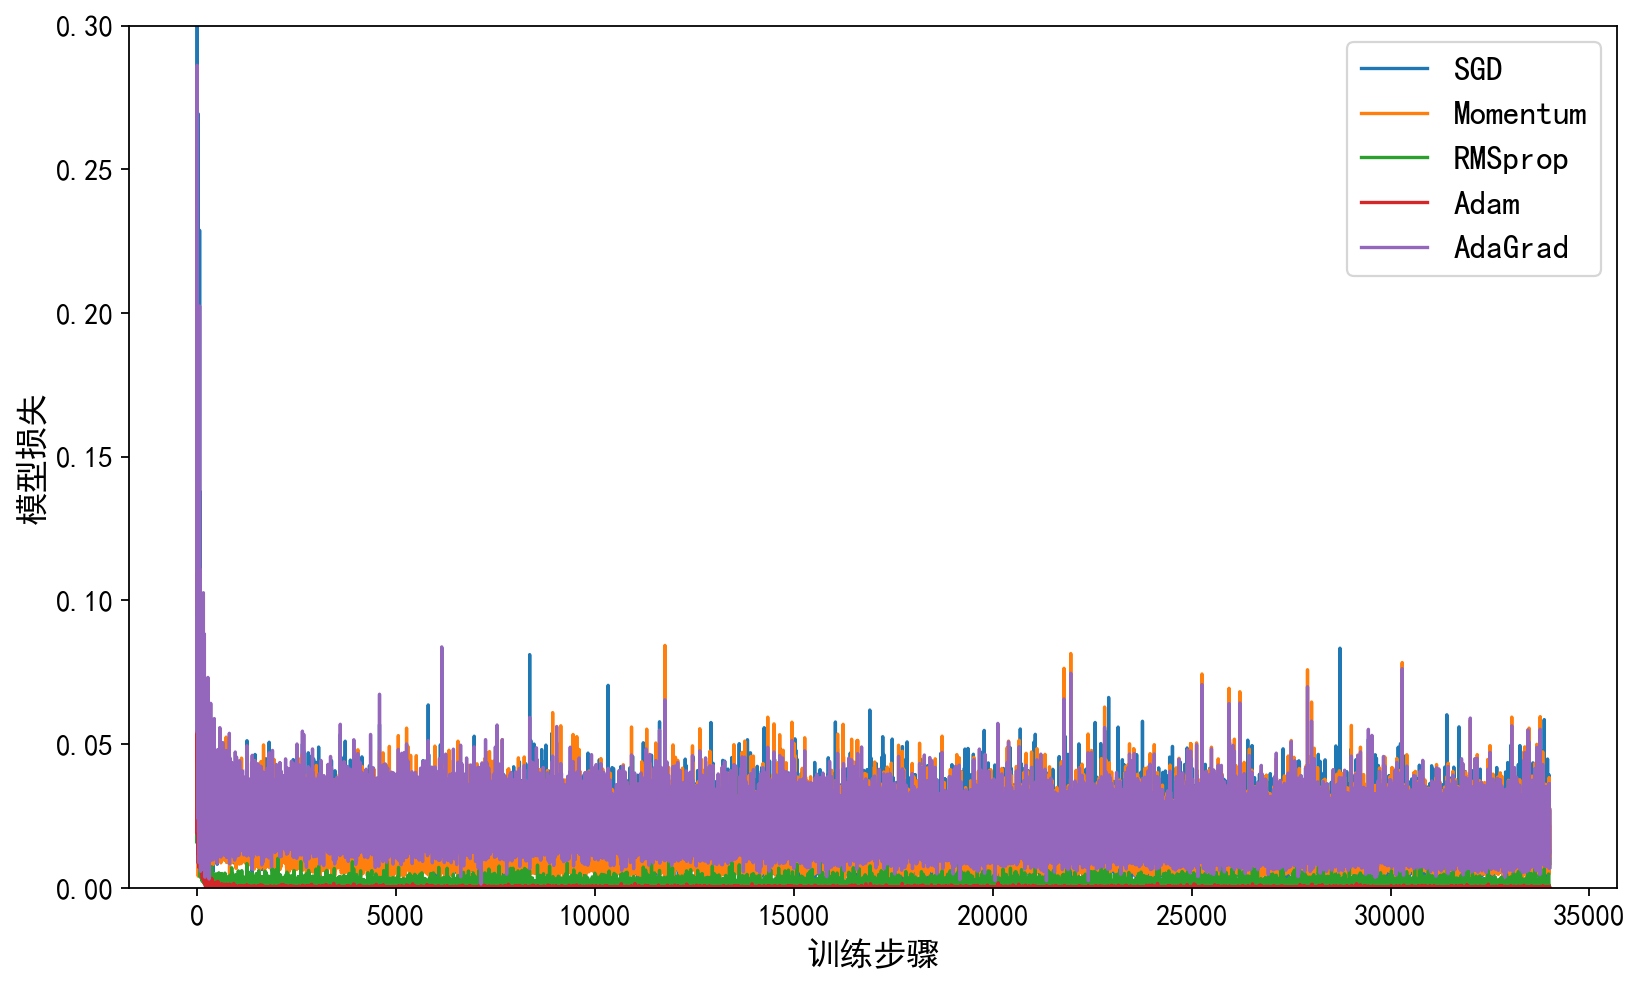
\includegraphics[width=0.6\textwidth]{part/人工智能/深度学习框架/pic/Pytorch/PyTorch神经网络工具/多种优化器比较.png}
    \caption{多种优化器比较}
    \label{fig:Pytorch_Multi_Optimizers_Comparison}
\end{figure}


\section{训练模型}
\label{subsec:Pytorch_train_model}
PyTorch训练模型主要包括加载数据集、损失计算、定义优化算法、反向传播、参数更新等主要步骤。
\subsection{加载和预处理数据集}
\label{subsubsec:Pytorch_load_and_preprocess_dataset}
可以使用PyTorch的数据处理工具，如\codeinline{torch.utils}和\codeinline{torchvision}等

\subsection{定义损失函数}
\label{subsubsec:Pytorch_define_loss_function}
可以通过自定义方法或使用PyTorch内置的损失函数定义损失函数，
如回归使用的\codeinline{loss\_fun=nn.MSELoss()},分类使用的\codeinline{nn.BCELoss}等损失函数


\subsection{定义优化方法}
\label{subsubsec:Pytorch_define_optimization_method}
PyTorch常用的优化方法都封装在\codeinline{torch.optim}中，
其设计很灵活，可以扩展为自定义的优化方法。

所有的优化方法都是继承了基类\codeinline{otim.Optimizer},并实现了自己的优化步骤。

如使用SGD优化器时，可设置\codeinline{optimizer = torch.optim.SGD(params,lr = 0.001)}。


\subsection{循环训练模型}
\label{subsubsec:Pytorch_loop_train_model}
\begin{enumerate}[label=\arabic*)]
    \item 设置为训练模式：
    调用\codeinline{model.train()}会把所有的module设置为训练模式。
    % \begin{lstlisting}[style=demostyle,numbers=none]
    % model.train()
    % \end{lstlisting}

    \item 梯度清零
    在默认情况下梯度是累加的，需要手工把梯度初始化或清零，调用\codeinline{optimizer.zero\_grad()}即可。

    \item 求损失值
    \begin{lstlisting}[style=demostyle,numbers=none]
    y_pred = model(x)
    loss = loss_fun(y_pred, y)
    \end{lstlisting}

    \item 反向传播(自动求导)
    调用\codeinline{loss.backward()}即可。

    \item 更新参数
    调用\codeinline{optimizer.step()}即可。
\end{enumerate}




\subsection{循环测试或验证模型}
\label{subsubsec:Pytorch_loop_test_or_validate_model}
\begin{enumerate}[label=\arabic*)]
    \item 设置为测试或验证模式：
    调用\codeinline{model.eval()}会把所有的\codeinline{training}属性设置为\codeinline{False}。

    \item 在不跟踪梯度的模式下计算损失值、预测值等
    \begin{lstlisting}[style=demostyle,numbers=none]
    with torch.no_grad():
        y_pred = model(x)
        loss = loss_fun(y_pred, y)
    \end{lstlisting}
\end{enumerate}

\subsubsection{比较model.train()和model.eval()的区别}
\label{subsubsubsec:Pytorch_compare_model_train_and_eval}
如果模型中有批量归一化(Batch Normalization, BH)层和dropout层，
需要在训练时添加\codeinline{model.train()},在测试时添加\codeinline{model.eval()}

其中\codeinline{model.train()}是保证BN层用每一批数据的均值和方差，
而\codeinline{model.eval()}是保证BN层用全部训练数据的均值和方差；

而对于dropout层,\codeinline{model.train()}是随机取一部分网络连接来训练更新参数，
而\codeinline{model.eval()}是利用所有网络连接。 

\subsection{可视化结果}
\label{subsubsec:Pytorch_visualize_results}

\section{正则化}
\label{subsec:Pytorch_regularization}
正则化是一种用于防止过拟合的技术，主要有L1正则化、L2正则化、Dropout等方法。
\subsection{L1正则化}
\label{subsubsec:Pytorch_L1_regularization}

\subsection{L2正则化}
\label{subsubsec:Pytorch_L2_regularization}

\subsection{Dropout}
\label{subsubsec:Pytorch_dropout}

\subsection{Batch Normalization}
\label{subsubsec:Pytorch_batch_normalization}

\section{训练技巧}
\label{subsec:Pytorch_training_techniques}


\section{保存和加载模型}
\label{subsec:Pytorch_save_and_load_model}
PyTorch中保存和加载模型的方法有多种，如保存和加载整个模型、保存和加载模型参数等。


\section{实例}
\label{subsec:Pytorch_nn_tools_example}
\subsection{模拟余弦函数曲线}
\label{subsubsec:Pytorch_simulate_cosine_curve}
\begin{lstlisting}[style=pythonstyle]
# 导入相关第三方库
import torch
import torch.nn as nn
from torch.utils.data import DataLoader
from torch.utils.data import TensorDataset
import numpy as np
import matplotlib
import matplotlib.pyplot as pit
matplotlib.rcParams['font.sans-serif'] = ['SimHei']
matplotlib.rcParams['axes.unicode_minus'] = False

# 准备拟合数据
x=np.linspace(-2*np.pi, 2*np.pi, 400)
y=np.cos(x)
X=np. expand_dims (x, axis=1)
Y=y.reshape(400,-1)
dataset=TensorDataset(torch.tensor(X,dtype=torch.float) , torch.tensor(Y,dtype=torch.float))
dataloader=DataLoader(dataset,batch_size=10,shuffle=True)

# 设置神经网络，这里就用一个简单的线性结构
class Net(nn.Module):
    def __init__(self):
        super(Net, self).__init__()
        self.net=nn.Sequential(
            nn.Linear(1,100),
            nn.ReLU(),
            nn.Linear(100,1)
        )
    def forward(self, input:torch.FloatTensor):
        return self.net(input)
    
net=Net()    

# 设置优化器和损失函数 
optim=torch.optim.Adam(Net.parameters(net),lr=0.001)
Loss=nn.MSELoss()

# 开始训练  
epochs=1000
for epoch in range(epochs):
    loss=None
    for batch_x, batch_y in dataloader:
        y_predict=net(batch_x)
        loss=Loss(y_predict, batch_y)
        optim.zero_grad()
        loss.backward()
        optim.step()
    if epoch%100==0:
        print(f'epoch:{epoch},loss:{loss.item()}')

predict=net(torch.tensor(X,dtype=torch.float))
# 可视化结果
pit.figure(figsize=(12, 7), dpi=160)
pit.plot(x, y, label="实际值", marker = "X")
pit.plot(x, predict.detach().numpy(), label="预测值", marker= 'o')
pit.xlabel("x", size=15)
pit.ylabel ("cos (x)", size=15)
pit.xticks(size=15)
pit.yticks(size=15)
pit.legend(fontsize=15)
pit.show()    
\end{lstlisting}
\begin{lstlisting}[style=demostyle,numbers=none]
epoch:0,loss:0.413939893245697
epoch:100,loss:0.005030750297009945
epoch:200,loss:0.0018504426116123796
epoch:300,loss:0.0018474120879545808
epoch:400,loss:0.0006889037904329598
epoch:500,loss:0.0005864549311809242
epoch:600,loss:0.0002862799447029829
epoch:700,loss:0.001682802801951766
epoch:800,loss:0.0007093378226272762
epoch:900,loss:3.737903170986101e-05
\end{lstlisting}    
\begin{figure}[htpb]
    \centering
    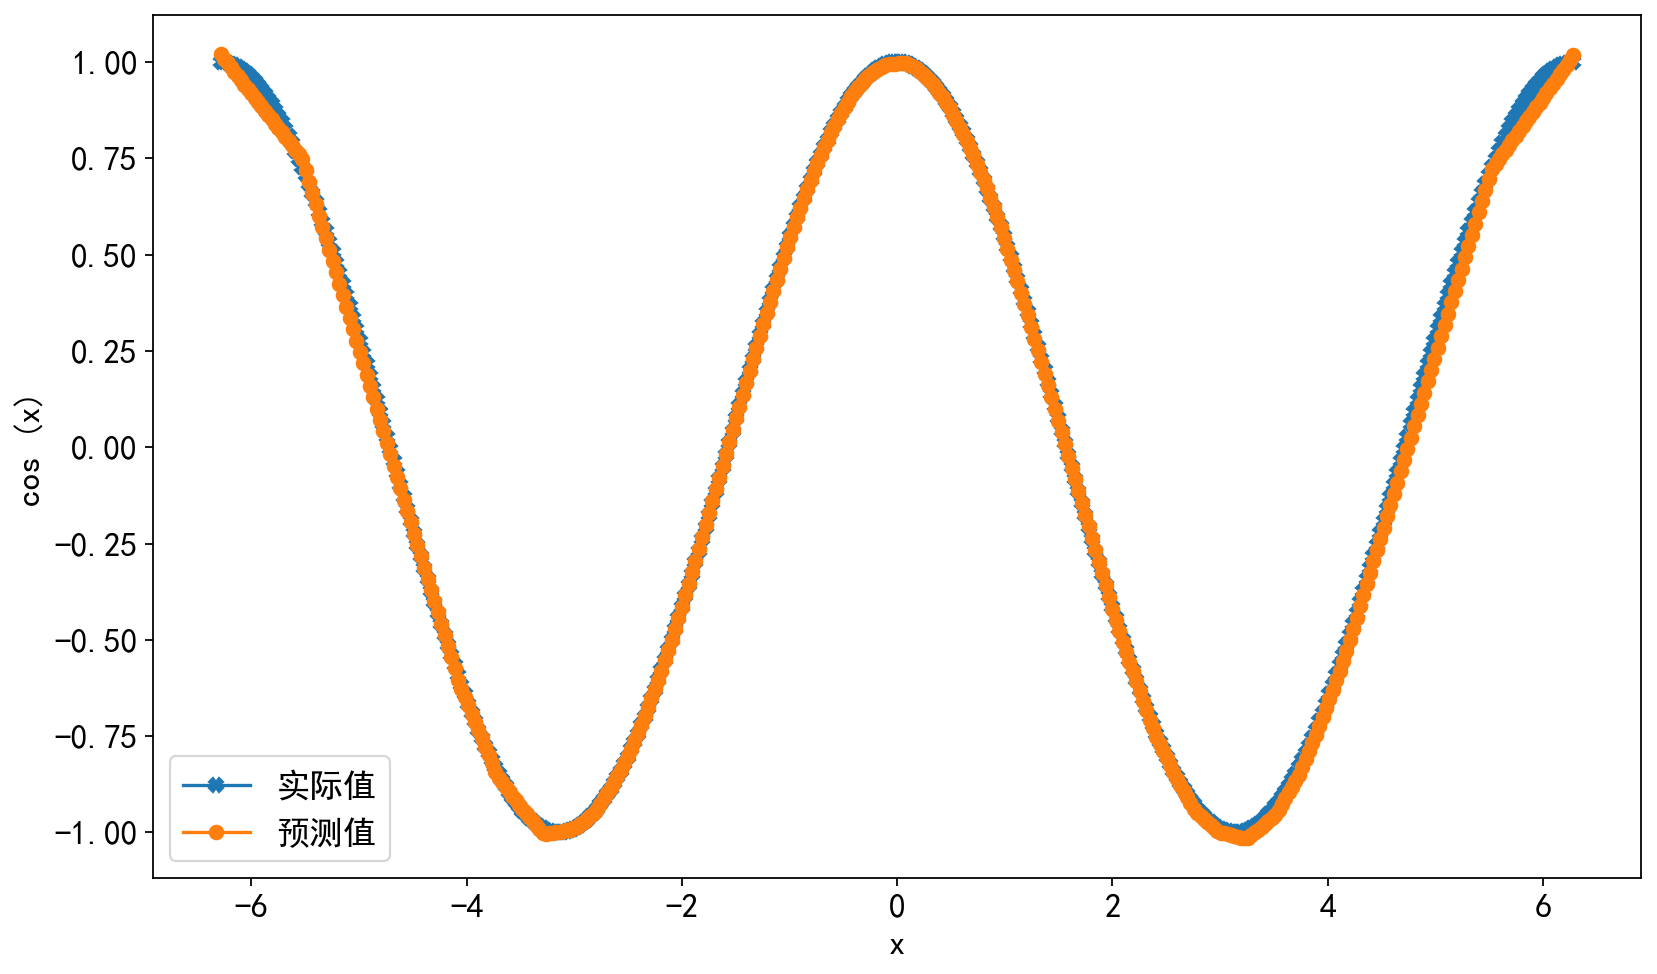
\includegraphics[width=0.6\textwidth]{part/人工智能/深度学习框架/pic/Pytorch/PyTorch神经网络工具/模拟余弦函数曲线.png}
    \caption{模拟余弦函数曲线}
    \label{fig:Pytorch_simulate_cosine_curve}
\end{figure}






\input{part/人工智能/深度学习框架/Pytorch/PyTorch可视化.tex}

% \part{深度学习应用}
% \input{part/深度学习应用/推荐算法.tex}
% \input{part/深度学习应用/语音识别.tex}
% \input{part/深度学习应用/模式识别.tex}
% \input{part/深度学习应用/目标检测.tex}
% \input{part/深度学习应用/智慧城市.tex}
\part{办公自动化}
\chapter{excel自动化概述}
\label{cha:excel自动化}
Python操作excel的库有\href{https://xlrd.readthedocs.io/en/latest/}{xlrd}、
\href{https://xlwt.readthedocs.io/en/latest/}{xlwt}、\href{https://openpyxl.readthedocs.io/en/stable/}{openpyxl}、\href{https://xlutils.readthedocs.io/en/latest/}{xlutils}。

\section{Excel介绍}
\label{sec:Excel介绍}
Excel工作簿有两种格式:\codeinline{xls}和\codeinline{xlsx}。
\reminder{\lefthand}{如果存储的数据大于工作簿的极限时，就可以考虑使用数据库来存储数据。}


\begin{enumerate}[label=\arabic*)]
    \item \codeinline{xls}格式的文件是二进制文件，它是Excel 2003及以前版本的文件格式。

    \codeinline{xls}格式的文件最多可写入65 535行、256列的数据量

    \item \codeinline{xlsx}格式的文件是XML文件，它是Excel 2007及以后版本的文件格式。    

    \codeinline{xlsx}格式的文件最多可写入1048576行、16384列的数据量    
\end{enumerate}


\section{处理Excel文件的Python模块}
可以处理Excel文件的Python模块有很多，如XlsxWriter、xlrd、xlwt、xlutils、openpyxl和xlwings等。

\begin{table}[htbp]
\centering
\begin{tabular}{|c|c|c|c|c|c|c|}
\hline
\textbf{功能$\backslash$ 模块} & \textbf{XlsxWriter} & \textbf{xlrd} & \textbf{xlwt} & \textbf{xlutils} & \textbf{openpyxl} & \textbf{xlwings} \\ \hline
\textbf{读} & $x$ & \checkmark & $x$ & \checkmark & \checkmark & \checkmark \\ \hline
\textbf{写} & \checkmark & $x$ & \checkmark & \checkmark & \checkmark & \checkmark \\ \hline
\textbf{修改} & $x$ & $x$ & $x$ & \checkmark & \checkmark & \checkmark \\ \hline
\textbf{支持 xls 格式} & $x$ & \checkmark & \checkmark & \checkmark & $x$ & \checkmark \\ \hline
\textbf{支持 xlsx 格式} & \checkmark & \checkmark & \checkmark & $x$ & \checkmark & \checkmark \\ \hline
\textbf{支持批量操作} & $x$ & $x$ & $x$ & $x$ & $x$ & \checkmark \\ \hline
\end{tabular}
\caption{python Excel 不同模块支持功能情况}
\end{table}

通过上表的对比可以发现，xlwings模块的功能是最齐全的。
它不仅能读、写和修改两种格式的Excel文件（xls和xlsx），而且能批量处理多个Excel文件。
此外，xlwings模块还能与Excel VBA结合使用，实现更加强大的数据输入和分析功能。




















\chapter{Pandas处理Excel}
与NumPy模块相比，pandas模块更擅长处理二维数据，其主要有\codeinline{Series}和\codeinline{DataFrame}两种数据结构。

\section{Excel文件操作}
\subsection{read\_excel 文件读取}
通过pandas模块可以从多种格式的数据文件中读取数据，也可以将处理后的数据写入这些文件中。
\begin{lstlisting}[style=demostyle,numbers=none]
import pandas as pd
df = pd.read_excel('xlsx文件')

# 或者
df = pd.read_excel('xlsx文件', sheetname='工作表名', endcoding='utf-8')
df = pd.read_excel('xlsx文件', sheetname=0, endcoding='utf-8',index_col=0)
## sheetname用于指定工作表，可以是工作表名称，也可以是数字（默认为0，即第1个工作表）
## encoding用于指定编码格式，默认为utf-8
## index_col用于指定索引列，默认为0，即第一列作为索引
\end{lstlisting}

除了读取Excel工作簿，pandas模块还可以读取CSV文件。
CSV文件本质上是一个文本文件，它仅存储数据，不能像Excel工作簿那样存储格式、公式、宏等信息，
所以所占存储空间通常较小。
CSV文件一般用逗号分隔一系列值，既可以用Excel打开，也可以用文本编辑器（如“记事本”）打开。
\begin{lstlisting}[style=demostyle,numbers=none]
# 读取csv文件
df = pd.read_csv('csv文件')

# 或者
data = pd.read_csv('csv文件.csv', delimiter=',', encoding='utf-8')
## delimiter用于指定分隔符，默认为逗号
## encoding用于指定编码格式，默认为utf-8
\end{lstlisting}

\subsection{DataFrame.to\_excel 文件写入}
\begin{lstlisting}[style=demostyle,numbers=none]
import pandas as pd   

DataFrame.to_excel('xlsx文件')

# 或者
DataFrame.to_excel('xlsx文件', sheet_name='工作表名', encoding='utf-8', index=False)
## sheet_name用于指定工作表名称，默认为'Sheet1'
## encoding用于指定编码格式，默认为utf-8
## index=False用于不写入索引列

DataFrame.to_excel('xlsx文件',index=['A','B','C'])
\end{lstlisting}        

\begin{figure}[htbp]
\centering
\begin{minipage}[t]{0.3\textwidth}
  \centering
  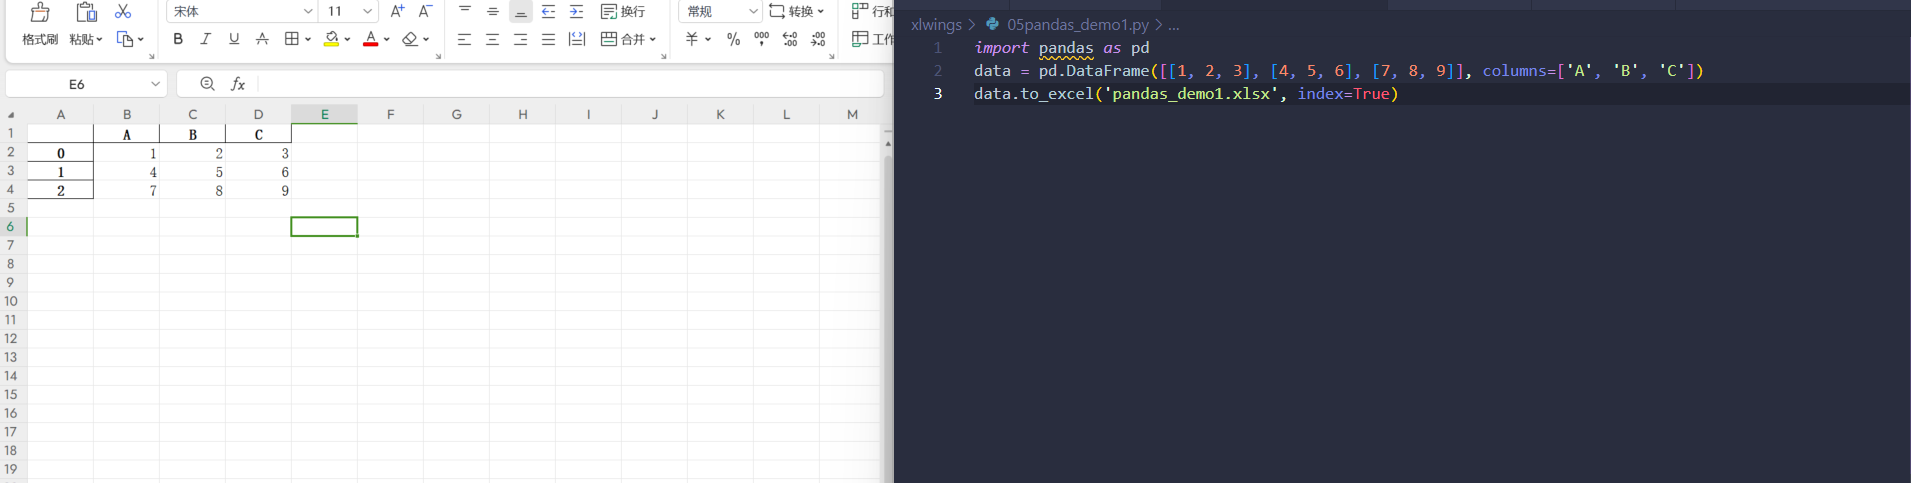
\includegraphics[width=0.7\linewidth]{part/自动化/办公自动化/pic/excel/pandas/pandas写入xlsx写入index.png}
  \caption{index=True}
\end{minipage}
\hspace{0.1\textwidth} % 调整这里的参数来改变图片之间的空隙
\begin{minipage}[t]{0.3\textwidth}
  \centering
  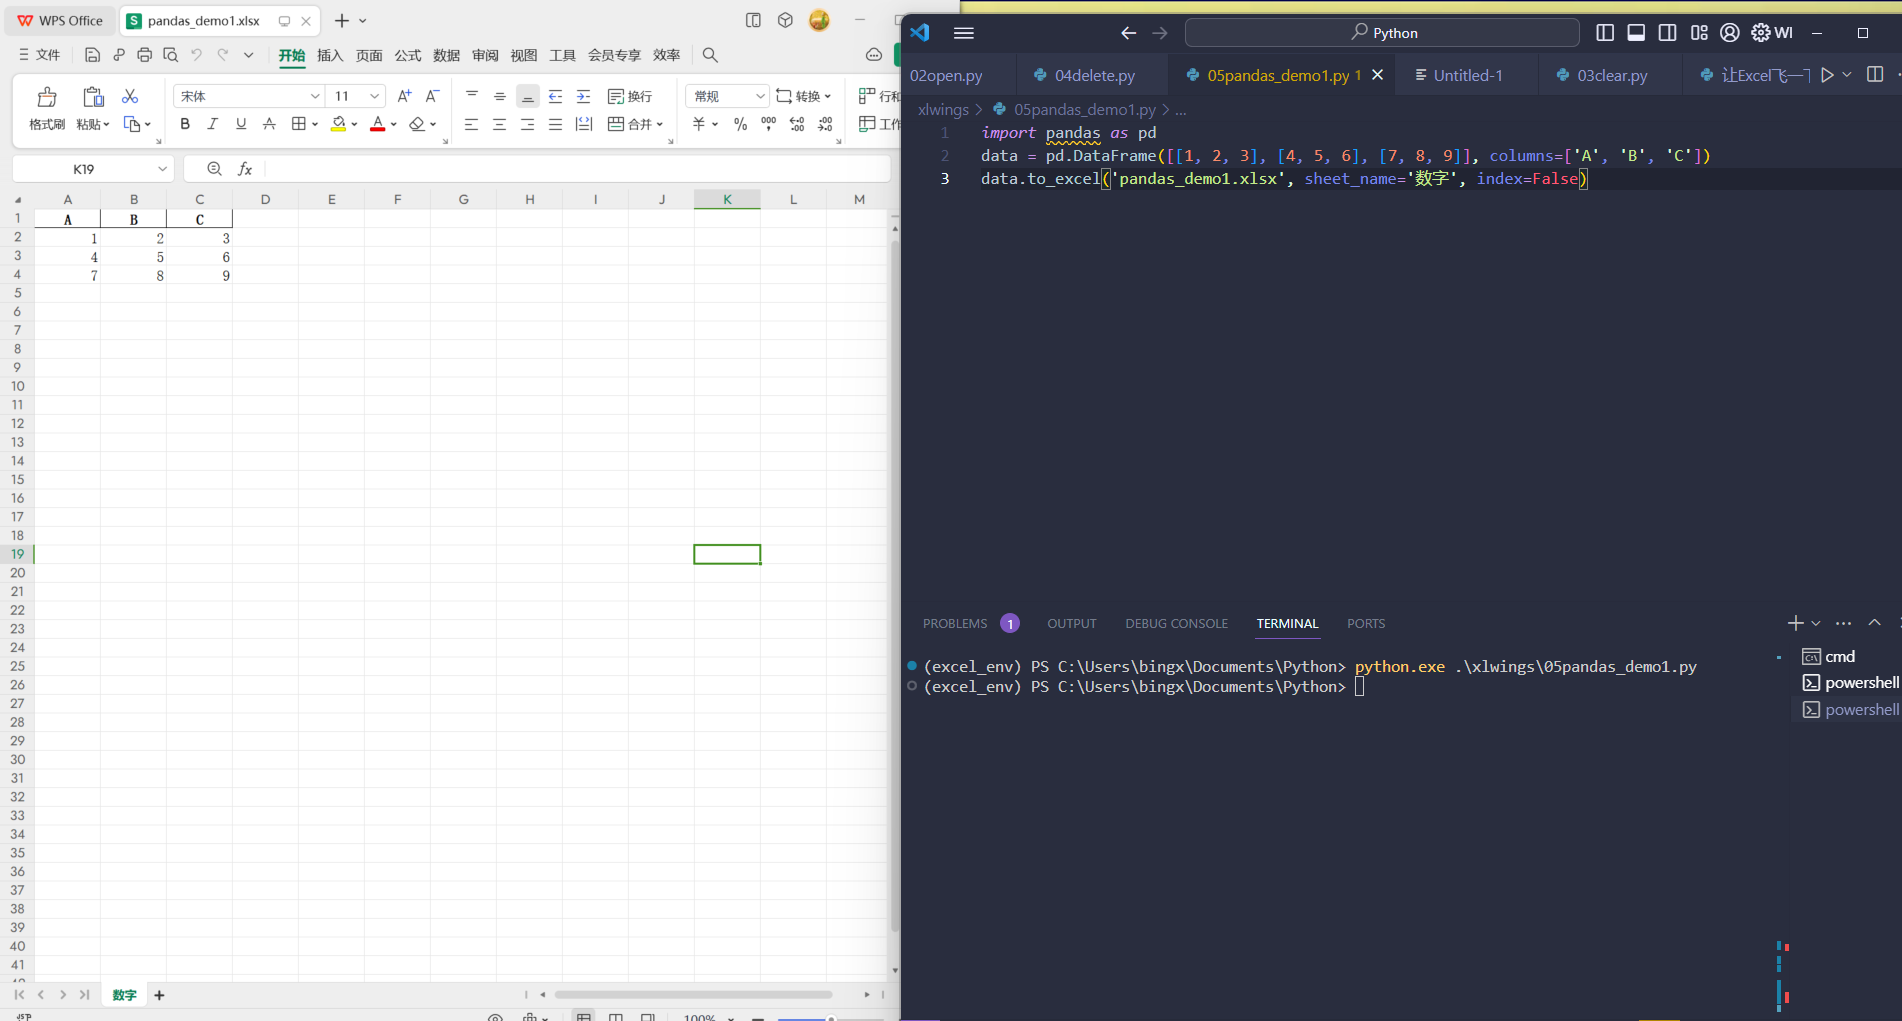
\includegraphics[width=0.7\linewidth]{part/自动化/办公自动化/pic/excel/pandas/pandas写入xlsx指定sheet名不写入index.png}
  \caption{sheetname='数字',index=False}
\end{minipage}
\caption{pandas写入Excel}
\end{figure}

\section{Sheet工作表(sheet)}
\subsection{读取工作表(sheet)}
\begin{lstlisting}[style=demostyle,numbers=none]
# 读取工作表(sheet)
df = pd.read_excel('xlsx文件', sheet_name='工作表名')
\end{lstlisting}

\subsection{写入工作表(sheet)}
\begin{lstlisting}[style=demostyle,numbers=none]
# 写入工作表(sheet)
df.to_excel('xlsx文件', sheet_name='工作表名')

# 写入多个 Sheet：pd.ExcelWriter
with pd.ExcelWriter('xlsx文件') as writer:
    df1.to_excel(writer, sheet_name='Sheet1')
    df2.to_excel(writer, sheet_name='Sheet2')
\end{lstlisting}

\section{Cell单元格}
Pandas \textcolor{red}{\textbf{不直接}}提供单元格级别操作，但可以通过 DataFrame 来间接实现：
\subsection{获取单元格}
\subsubsection{按行/列索引获取单元格}
\begin{enumerate}[label=\arabic*)]
    \item \codeinline{df['列名']}: 获取整列数据
    \item \codeinline{df[['列名1', '列名2']]}: 获取多列数据
    \item \codeinline{df.iloc[行索引]}: 获取整行数据
    \item \codeinline{df.iloc[[行索引1, 行索引2]]}: 获取多行数据
    \item \codeinline{df.head(n)}: 获取前n行数据
\end{enumerate}

\subsubsection{按区块获取单元格}
\begin{enumerate}[label=\arabic*)]
    \item \codeinline{df['列名'][行索引]}: 先根据列名获取列数据，再根据行索引获取单元格数据
    \item \codeinline{df.iloc[行索引][列索引]}: 先根据行索引获取行数据，再根据列索引获取单元格数据
\end{enumerate}

\subsection{数据筛选}
\begin{lstlisting}[style=demostyle,numbers=none]
import pandas as pd  
df = pd.read_excel('xlsx文件')
df[df['列名'] > 0] # 筛选列名大于0的行  

# 多条件筛选
df[(df['列名1'] > 0) & (df['列名2'] > 0)] # 筛选列名1和列名2都大于0的行
\end{lstlisting}

\subsection{sort\_values 排序}  
\begin{lstlisting}[style=demostyle,numbers=none]
import pandas as pd  
df = pd.read_excel('xlsx文件')
df.sort_values('列名', ascending=True) # 升序排序
df.sort_values('列名', ascending=False) # 降序排序
\end{lstlisting}

\subsection{数据运算}
\begin{lstlisting}[style=demostyle,numbers=none]
import pandas as pd  
df = pd.read_excel('xlsx文件')
df['新的列名'] = df['列名1'] + df['列名2'] # 列名1和列名2相加
df['新的列名'] = df['列名1'] - df['列名2'] # 列名1和列名2相减
df['新的列名'] = df['列名1'] * df['列名2'] # 列名1和列名2相乘
df['新的列名'] = df['列名1'] / df['列名2'] # 列名1和列名2相除
\end{lstlisting}

\subsection{drop 删除行/列}
\begin{lstlisting}[style=demostyle,numbers=none]
import pandas as pd  
df = pd.read_excel('xlsx文件')
df.drop(0) # 删除第一行
df.drop([0, 1]) # 删除第一行和第二行
df.drop('列名') # 删除列名对应的列
\end{lstlisting}


\subsection{数据表的拼接}
\subsubsection{merge 拼接}
\codeinline{merge()}函数可以根据一个或多个同名的列将不同数据表中的行连接起来。
\begin{lstlisting}[style=demostyle,numbers=none]
pd.merge(left, right, how='inner', on='key_column')
# left和right是要连接的两个数据表
# how用于指定连接方式，inner（内连接）、outer（外连接）、left（左连接）、right（右连接）
# on用于指定连接的列名
\end{lstlisting}

\begin{lstlisting}[style=pythonstyle,numbers=left]
import pandas as pd

# 两个数据表
df1 = pd.DataFrame({'ID': [1, 2, 3], 'Name': ['Alice', 'Bob', 'Charlie']})
df2 = pd.DataFrame({'ID': [2, 3, 4], 'Score': [85, 90, 95]})
print("df1:{}\n".format(df1))
print("df2:{}\n".format(df2))


# 按 ID 列进行内连接
result = pd.merge(df1, df2, how='inner', on='ID')
print(result)
\end{lstlisting}
\begin{lstlisting}[style=demostyle,numbers=none]
df1:   ID     Name
0   1    Alice
1   2      Bob
2   3  Charlie

df2:   ID  Score
0   2     85
1   3     90
2   4     95

   ID     Name  Score
0   2      Bob     85
1   3  Charlie     90
\end{lstlisting}

\subsubsection{concat 全连接}
\codeinline{concat()}函数使用全连接（UNION ALL）方式完成拼接，
它不需要对齐，而是直接进行合并，
即不需要两个表有相同的列或索引，只是把数据整合到一起。

因此，该函数没有参数\codeinline{how}和\codeinline{on}，而是用参数\codeinline{axis}指定连接的轴向。
该参数默认值为0，指按行方向连接（纵向拼接）。

\begin{lstlisting}[style=demostyle,numbers=none]
pd.concat([df1, df2], axis=0)
# axis=0表示按行方向连接（纵向拼接）
# axis=1表示按列方向连接（横向拼接）
\end{lstlisting}

\begin{lstlisting}[style=pythonstyle,numbers=left]
import pandas as pd
# 两个数据表
df1 = pd.DataFrame({'A': [1, 2], 'B': [3, 4]})
df2 = pd.DataFrame({'A': [5, 6], 'B': [7, 8]})
print("df1:{}\n".format(df1))
print("df2:{}\n".format(df2))

# 按行拼接
result_row = pd.concat([df1, df2], axis=0, ignore_index=True)

# 按列拼接
result_col = pd.concat([df1, df2], axis=1)
print("按行拼接:")
print(result_row)
print("\n按列拼接:")
print(result_col)
\end{lstlisting}
\begin{lstlisting}[style=demostyle,numbers=none]
df1:   A  B
0  1  3
1  2  4

df2:   A  B
0  5  7
1  6  8

按行拼接:
   A  B
0  1  3
1  2  4
2  5  7
3  6  8

按列拼接:
   A  B  A  B
0  1  3  5  7
1  2  4  6  8
\end{lstlisting}


\subsubsection{append 纵向拼接}
\codeinline{append()} 是 \codeinline{concat()} 的简化版本，通常用于按行追加数据(\codeinline{axis=0})。

\begin{lstlisting}[style=demostyle,numbers=none]
df1.append(df2, ignore_index=True)
# ignore_index=True表示忽略原索引，生成新的索引
\end{lstlisting}
\begin{lstlisting}[style=pythonstyle,numbers=left]
import pandas as pd
# 两个数据表
df1 = pd.DataFrame({'A': [1, 2], 'B': [3, 4]})
df2 = pd.DataFrame({'A': [5, 6], 'B': [7, 8]})
print("df1:{}\n".format(df1))
print("df2:{}\n".format(df2))
result = df1._append(df2, ignore_index=True)
print(result)
result = df1._append(df2, ignore_index=False)
print(result)
\end{lstlisting}
\begin{lstlisting}[style=demostyle,numbers=none]
df1:   A  B
0  1  3
1  2  4

df2:   A  B
0  5  7
1  6  8

   A  B
0  1  3
1  2  4
2  5  7
3  6  8

   A  B
0  1  3
1  2  4
0  5  7
1  6  8
\end{lstlisting}

\chapter{[麻烦] xlrd、xlwt与xlutils库}
\label{sec:xlrd与xlwt库}
\reminder{\lefthand}{\codeinline{xlrd} 和 \codeinline{xlwt} 分别是读取和写入，但是如果需要修改工作簿中的数据，就需要使用 \codeinline{xlutils} 库。\\
如果只靠 \codeinline{xlrd} 和 \codeinline{xlwt} 来修改工作簿中的数据，其过程会很复杂，
需要通过xlrd获取工作簿中所有的数据，
然后通过xlwt建立新的工作簿，
再将xlrd读取的数据写入，在写入的过程中修改数据}

\begin{enumerate}[label=\arabic*)]
        \item \codeinline{xlrd}:\\
         支持Excel 读取的扩展库\\
         支持 \codeinline{xls}和\codeinline{xlsx}格式的文件\\

     \item \codeinline{xlwt}:\\
         支持Excel 写入的扩展库\\
         \textcolor{red}{\textbf{仅}}支持 \codeinline{xls}格式的文件\\
     \item \codeinline{xlutils}\\
         用于Excel修改的扩展库\\
         \textcolor{red}{\textbf{仅}}支持 \codeinline{xls}格式的文件\\
         而且需要安装 \codeinline{xlrd} 和 \codeinline{xlwt} 才能使用\\
        \codeinline{xlutils} 是一个用于读取、写入和复制 Excel 文件的库，它是 \codeinline{xlrd} 和 \codeinline{xlwt} 的结合体。

        xlutils依赖于xlrd与xlwt,它最常用的功能就是将xlrd的Book对象复制成xlwt的
Workbook对象，从而实现xlrd与xlwt之间的数据流通，它起到了 “桥梁”的作用。
\end{enumerate}


\section{安装}
\label{subsec:xlrd与xlwt与xlutils库安装}
\begin{lstlisting}[style=demostyle,numbers=none]
# pip 安装
pip install xlrd
pip install xlwt

# conda 安装
conda install xlrd
conda install xlwt
# 在安装xlutils之前，需要先安装xlrd与xlwt
# pip 安装
pip install xlutils

# conda 安装
conda install xlutils
\end{lstlisting}

\section{读取Excel内容}
\label{subsec:xlrd读取Excel内容}
\begin{lstlisting}[style=demostyle,numbers=none]
# xlrd 的函数
xlrd.open_workbook(file)              # 打开文件
xlrd.open_workbook().sheets()         # 获取工作簿中所有的sheet
xlrd.open_workbook().sheet_names()    # 获取sheet的名字
xlrd.open_workbook().sheets_count()   # 获取sheet的个数
xlrd.open_workbook().sheet_by_index() # 根据索引获取sheet
xlrd.open_workbook().sheet_by_name('Sheet name')  # 根据名字获取sheet
xlrd.open_workbook().sheets().nrows   # 获取sheet的行数
xlrd.open_workbook().sheets().ncols   # 获取sheet的列数
xlrd.open_workbook().sheets().cell_value(rowx, colx) # 获取单元格的值
\end{lstlisting}

\begin{lstlisting}[style=pythonstyle,numbers=left]
import xlrd 

file = r"C:\Users\tony\Documents\Pythonauto\excel\example.xls"
## r :告诉Python不对反斜杠进行转义(windows独有)
## 这里要使用xls格式的文件，如果是xlsx格式的文件，需要使用openpyxl库

wb = xlrd.open_workbook(file)
# 获取全部的sheet
sheets = xlrd.open_workbook(file).sheets()
print(sheets)

# 使用wb.sheet_by_index() 来获取sheet
sheet = wb.sheet_by_index(0)
# 打印sheet的名字
print("sheet 的名字是", sheet.name)
# 打印sheet的行数
print("sheet 的行数是", sheet.nrows)
# 打印sheet的列数
print("sheet 的列数是", sheet.ncols)
# 打印第一行的值
print("第一行的值是", sheet.row_values(0))
# 打印第一列的值
print("第一列的值是", sheet.col_values(0))
# 打印第一行第一列的值
print("第一行第一列的值是", sheet.cell_value(0, 0))

# 使用wb.sheets() 来获取sheet
table = wb.sheets()[1]
print("sheet 的名字是", table.name)
print("sheet 的行数是", table.nrows)
print("sheet 的列数是", table.ncols)
print("第一行的值是", table.row_values(0))
print("第一列的值是", table.col_values(0))
# 打印第二行第三列的值
print("第二行第三列的值是", table.cell_value(1, 2))

# 使用wb.sheet_by_name() 来获取sheet
sheets_teacher = wb.sheet_by_name("教师")
sheets_tea_nrows = sheets_teacher.nrows
sheets_tea_ncols = sheets_teacher.ncols
for i in range(sheets_tea_nrows):
    for j in range(sheets_tea_ncols):
        print(sheets_teacher.cell_value(i, j), end="\t")
    print()
\end{lstlisting}


\section{写入Excel内容}
\label{subsec:xlwt写入Excel内容}
\begin{lstlisting}[style=demostyle,numbers=none]
# xlwt 的函数
## Workbook() 创建一个工作簿
## add_sheet() 创建一个工作表
## write() 写入数据
## save() 保存数据
\end{lstlisting}

\begin{lstlisting}[style=pythonstyle,numbers=left]
import xlwt

file = r"C:\Users\tony\Documents\Pythonauto\excel\example1.xls"

# 创建一个workbook对象，相当于创建一个Excel文件
wb = xlwt.Workbook()
# 创建一个sheet对象，相当于创建一个sheet
sheet = wb.add_sheet("第一个sheet")

# 写入数据
# 写入第一行
sheet.write(0, 0, "姓名")
sheet.write(0, 1, "年龄")
sheet.write(0, 2, "性别")
# 写入第二行
sheet.write(1, 0, "张三")
sheet.write(1, 1, 18)
sheet.write(1, 2, "男")

# 创建第二个sheet
sheet1 = wb.add_sheet("第二个sheet")
# 写入数据
# 写入第一行
sheet1.write(0, 0, "姓名")
sheet1.write(0, 1, "年龄")
sheet1.write(0, 2, "性别")
# 写入第二行
sheet1.write(1, 0, "李四")
sheet1.write(1, 1, 20)
sheet1.write(1, 2, "女")

# 保存文件
wb.save(file
\end{lstlisting}

\section{类型转换}
\label{subsec:xlrd类型转换}
当读取Excel文件时，\codeinline{xlrd}库会将所有的数据都当做字符串来处理，如果需要将数据转换为其他类型，可以使用\codeinline{int()}、\codeinline{float()}等函数进行转换。

\begin{lstlisting}[style=demostyle,numbers=none]
#Python 中没有与工作簿中日期格式相对应的数据类型，所以日期格式的数据会被读取为浮点数
# 如果直接使用 cell_value 会将日期转换为浮点数，需要使用 xldate_as_tuple() 函数将日期转换为元组或者使用 xldate_as_datetime() 函数将日期转换为 datetime 对象

# xldate_as_tuple() 函数将日期转换为元组
time_tuple = xlrd.xldate_as_tuple(cell.value, workbook.datemode) # 将日期转换为元组
# 将日期元组转换为字符串
time_str = datetime(*time_tuple).strftime('%Y-%m-%d')

# xldate_as_datetime() 函数将日期转换为 datetime 对象
time_value = xlrd.xldate_as_datetime(cell.value, workbook.datemode) # 将日期转换为datetime对象
# 将日期对象转换为字符串
time_str = time_value.strftime('%Y-%m-%d')
## datemode 参数指示日期模式，它有两个可能的值：
## 0：1900年作为基准，Excel for Windows的默认模式,Excel日期值减去1
## 1：1904年作为基准，Excel for Mac的默认模式,Excel日期值减去1

# 如果单元格的数据类型是布尔类型，可以使用 cell.ctype == xlrd.XL_CELL_BOOLEAN 来判断
if cell.ctype == xlrd.XL_CELL_BOOLEAN:
    print(cell.value)
    sheet.write(row, col, xlwt.Formula('TRUE')) # 写入布尔值

# easyxf() 函数可以设置单元格的样式
xlwt.easyxf(num_format_str='YYYY-MM-DD') # 设置日期格式以 "年-月-日" 的形式显示
xlwt.easyxf(num_format_str='BOOLEAN') # 设置布尔格式，显示为 TRUE 或 FALSE

\end{lstlisting}

\begin{lstlisting}[style=pythonstyle,numbers=left]
import xlwt, xlrd
from datetime import datetime

# 创建一个新的Excel工作簿
workbook = xlwt.Workbook()

# 创建第一个工作表，包含字符串和数字
sheet1 = workbook.add_sheet('包含字符串和数字')
sheet1.write(0, 0, 'Name')
sheet1.write(0, 1, 'Age')
sheet1.write(1, 0, 'Alice')
sheet1.write(1, 1, 30)
sheet1.write(2, 0, 'Bob')
sheet1.write(2, 1, 25)

# 创建第二个工作表，包含日期类型
sheet2 = workbook.add_sheet('包含日期')
sheet2.write(0, 0, 'Event')
sheet2.write(0, 1, 'Date')
date_style = xlwt.easyxf(num_format_str='YYYY-MM-DD')
sheet2.write(1, 0, 'Conference')
sheet2.write(1, 1, datetime(2023, 6, 15), date_style)
sheet2.write(2, 0, 'Meeting')
sheet2.write(2, 1, datetime(2023, 7, 20), date_style)

# 创建第三个工作表，包含布尔类型
sheet3 = workbook.add_sheet('包含布尔值')
sheet3.write(0, 0, 'Task')
sheet3.write(0, 1, 'Completed')
sheet3.write(1, 0, 'Task1')
sheet3.write(1, 1, xlwt.Formula('TRUE'))
sheet3.write(2, 0, 'Task2')
sheet3.write(2, 1, xlwt.Formula('FALSE'))

# 保存工作簿
workbook.save('不同类型的excel.xls')

# 打开之前创建的Excel文件
workbook = xlrd.open_workbook('不同类型的excel.xls')

# 读取第一个工作表
sheet1 = workbook.sheet_by_name('包含字符串和数字')
print("Sheet1 ", sheet1.name, "Data:")
for row in range(sheet1.nrows):
    for col in range(sheet1.ncols):
        print(sheet1.cell_value(row, col), end=' ')
    print()

# 读取第二个工作表
sheet2 = workbook.sheet_by_name('包含日期')
print("\nSheet2 ", sheet2.name, "Data:")
for row in range(sheet2.nrows):
    for col in range(sheet2.ncols):
        cell = sheet2.cell(row, col)
        if cell.ctype == xlrd.XL_CELL_DATE:
            #date_value = xlrd.xldate_as_tuple(cell.value, workbook.datemode) # 将日期转换为元组
            # print(datetime(*date_value).strftime('%Y-%m-%d'), end=' ') # 将日期元组转换为字符串
            # 或者使用 
            data_value = xlrd.xldate_as_datetime(cell.value, workbook.datemode) # 将日期转换为datetime对象
            print(data_value.strftime('%Y-%m-%d'), end=' ')
        else:
            print(cell.value, end=' ')
    print()

# 读取第三个工作表
sheet3 = workbook.sheet_by_name('包含布尔值')
print("\nSheet3 ", sheet3.name, "Data:")
for row in range(sheet3.nrows):
    for col in range(sheet3.ncols):
        print(sheet3.cell_value(row, col), end=' ')
    print()
\end{lstlisting}

\begin{figure}[htpb]
        \centering
        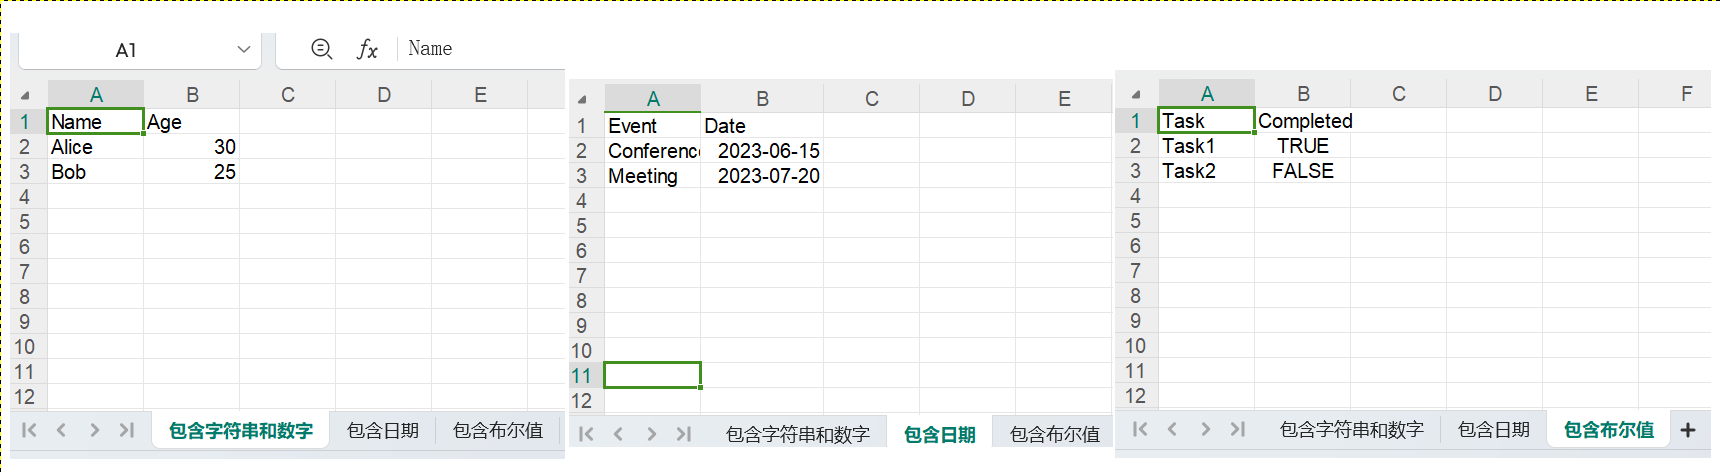
\includegraphics[width=0.8\textwidth]{part/自动化/办公自动化/pic/excel/数据类型转换结果演示.png}
        \caption{数据类型转换结果演示}
        \label{fig:数据类型转换结果演示}
\end{figure}

\begin{lstlisting}[style=demostyle,numbers=none]
Sheet1  包含字符串和数字 Data:
Name Age
Alice 30.0
Bob 25.0

Sheet2  包含日期 Data:
Event Date
Conference 2023-06-15
Meeting 2023-07-20

Sheet3  包含布尔值 Data:
Task Completed
Task1
Task2
\end{lstlisting}


\section{合并单元格}
\label{subsec:xlwt合并单元格}
\begin{lstlisting}[style=demostyle,numbers=none]
# 使用write_merge() 函数可以合并单元格
## write_merge(row1, row2, col1, col2, value, style)
## row1: 起始行
## row2: 结束行
## col1: 起始列
## col2: 结束列
## value: 写入的值
## style: 单元格样式
\end{lstlisting}

\begin{lstlisting}[style=pythonstyle,numbers=left]
import xlrd
import xlwt
from xlutils.copy import copy

# 打开现有的 Excel 文件
input_file = 'example.xls'
workbook = xlrd.open_workbook(input_file, formatting_info=True)
sheet = workbook.sheet_by_index(0)

# 创建一个新的工作簿，并将现有工作簿的内容复制到新的工作簿中
new_workbook = copy(workbook)
new_sheet = new_workbook.get_sheet(0)

# 合并单元格并设置内容
# 合并第2行第2列到第2行第4列的单元格（索引从0开始）
new_sheet.write_merge(1, 1, 1, 3, 'Merged Cell Content')

# 保存修改后的工作簿
output_file = 'merged_example.xls'
new_workbook.save(output_file)

print(f"合并单元格后的 Excel 文件已保存为 {output_file}")
\end{lstlisting}


\section{使用Excel函数}
\label{subsec:xlwt使用Excel函数}

\begin{lstlisting}[style=demostyle,numbers=none]
# 使用 xlwt.Formula() 函数可以在单元格中使用 Excel 函数
## 以下是一些常用的 Excel 函数
## SUM()：求和
## AVERAGE()：求平均值
## MAX()：求最大值
## MIN()：求最小值
## COUNT()：计数
## IF()：条件判断
## VLOOKUP()：垂直查找
## HLOOKUP()：水平查找
## CONCATENATE()：连接字符串
## LEFT()：提取字符串左边的字符
## RIGHT()：提取字符串右边的字符
## MID()：提取字符串中间的字符
## UPPER()：将字符串转换为大写
## LOWER()：将字符串转换为小写
## TRIM()：删除字符串两端的空格
## LEN()：计算字符串的长度
## DATE()：返回日期
## TIME()：返回时间
## NOW()：返回当前日期和时间
## RAND()：返回随机数
## PI()：返回圆周率
## SQRT()：求平方根
## POWER()：求幂
## LOG()：求对数
\end{lstlisting}

\begin{lstlisting}[style=pythonstyle,numbers=left]
import xlwt
from datetime import datetime

# 创建一个新的Excel工作簿
workbook = xlwt.Workbook()

# 数据样本
sample_data = [1, 2, 3, 4, 5]
lookup_data = [("A", 100), ("B", 200)]

# 演示SUM函数
sheet = workbook.add_sheet('演示SUM函数')
for row, value in enumerate(sample_data, start=1):
    sheet.write(row, 0, value)
sheet.write(0, 0, 'SUM')
sheet.write(0, 1, 'SUM(A2:A6)')
sheet.write(1, 2, xlwt.Formula('SUM(A2:A6)'))

# 演示AVERAGE函数
sheet = workbook.add_sheet('演示AVERAGE函数')
for row, value in enumerate(sample_data, start=1):
    sheet.write(row, 0, value)
sheet.write(0, 0, 'AVERAGE')
sheet.write(0, 1, 'AVERAGE(A2:A6)')
sheet.write(1, 2, xlwt.Formula('AVERAGE(A2:A6)'))

# 演示MAX函数
sheet = workbook.add_sheet('演示MAX函数')
for row, value in enumerate(sample_data, start=1):
    sheet.write(row, 0, value)
sheet.write(0, 0, 'MAX')
sheet.write(0, 1, 'MAX(A2:A6)')
sheet.write(1, 2, xlwt.Formula('MAX(A2:A6)'))

# 演示MIN函数
sheet = workbook.add_sheet('演示MIN函数')
for row, value in enumerate(sample_data, start=1):
    sheet.write(row, 0, value)
sheet.write(0, 0, 'MIN')
sheet.write(0, 1, 'MIN(A2:A6)')
sheet.write(1, 2, xlwt.Formula('MIN(A2:A6)'))

# 演示COUNT函数
sheet = workbook.add_sheet('演示COUNT函数')
for row, value in enumerate(sample_data, start=1):
    sheet.write(row, 0, value)
sheet.write(0, 0, 'COUNT')
sheet.write(0, 1, 'COUNT(A2:A6)')
sheet.write(1, 2, xlwt.Formula('COUNT(A2:A6)'))

# 演示IF函数
sheet = workbook.add_sheet('演示IF函数')
sheet.write(1, 0, 5)
sheet.write(0, 0, 'IF')
sheet.write(0, 1, 'IF(A2>10, "Greater than 10", "10 or less")')
sheet.write(1, 2, xlwt.Formula('IF(A2>10, "Greater than 10", "10 or less")'))

# 演示VLOOKUP函数
sheet = workbook.add_sheet('演示VLOOKUP函数')
for row, (key, value) in enumerate(lookup_data, start=6):
    sheet.write(row, 0, key)
    sheet.write(row, 1, value)
sheet.write(0, 0, 'VLOOKUP')
sheet.write(0, 1, 'VLOOKUP("B", $A$6:$B$7, 2, FALSE)')
sheet.write(1, 2, xlwt.Formula('VLOOKUP("B", $A$6:$B$7, 2, FALSE)'))

# 演示HLOOKUP函数
sheet = workbook.add_sheet('演示HLOOKUP函数')
for col, (key, value) in enumerate(lookup_data, start=6):
    sheet.write(0, col, key)
    sheet.write(1, col, value)
sheet.write(0, 0, 'HLOOKUP')
sheet.write(0, 1, 'HLOOKUP("B", $A$6:$B$7, 2, FALSE)')
sheet.write(2, 2, xlwt.Formula('HLOOKUP("B", $A$6:$B$7, 2, FALSE)'))

# 演示CONCATENATE函数
sheet = workbook.add_sheet('演示CONCATENATE函数')
sheet.write(1, 0, 'Hello')
sheet.write(1, 1, 'World')
sheet.write(0, 0, 'CONCATENATE')
sheet.write(0, 1, 'CONCATENATE(A2, " ", B2)')
sheet.write(1, 2, xlwt.Formula('CONCATENATE(A2, " ", B2)'))

# 演示LEFT函数
sheet = workbook.add_sheet('演示LEFT函数')
sheet.write(1, 0, 'Hello')
sheet.write(0, 0, 'LEFT')
sheet.write(0, 1, 'LEFT(A2, 3)')
sheet.write(1, 2, xlwt.Formula('LEFT(A2, 3)'))

# 演示RIGHT函数
sheet = workbook.add_sheet('演示RIGHT函数')
sheet.write(1, 0, 'Hello')
sheet.write(0, 0, 'RIGHT')
sheet.write(0, 1, 'RIGHT(A2, 3)')
sheet.write(1, 2, xlwt.Formula('RIGHT(A2, 3)'))

# 演示MID函数
sheet = workbook.add_sheet('演示MID函数')
sheet.write(1, 0, 'HelloWorld')
sheet.write(0, 0, 'MID')
sheet.write(0, 1, 'MID(A2, 2, 3)')
sheet.write(1, 2, xlwt.Formula('MID(A2, 2, 3)'))

# 演示UPPER函数
sheet = workbook.add_sheet('演示UPPER函数')
sheet.write(1, 0, 'hello')
sheet.write(0, 0, 'UPPER')
sheet.write(0, 1, 'UPPER(A2)')
sheet.write(1, 2, xlwt.Formula('UPPER(A2)'))

# 演示LOWER函数
sheet = workbook.add_sheet('演示LOWER函数')
sheet.write(1, 0, 'HELLO')
sheet.write(0, 0, 'LOWER')
sheet.write(0, 1, 'LOWER(A2)')
sheet.write(1, 2, xlwt.Formula('LOWER(A2)'))

# 演示TRIM函数
sheet = workbook.add_sheet('演示TRIM函数')
sheet.write(1, 0, '   Hello   ')
sheet.write(0, 0, 'TRIM')
sheet.write(0, 1, 'TRIM(A2)')
sheet.write(1, 2, xlwt.Formula('TRIM(A2)'))

# 演示LEN函数
sheet = workbook.add_sheet('演示LEN函数')
sheet.write(1, 0, 'Hello')
sheet.write(0, 0, 'LEN')
sheet.write(0, 1, 'LEN(A2)')
sheet.write(1, 2, xlwt.Formula('LEN(A2)'))

# 演示DATE函数
sheet = workbook.add_sheet('演示DATE函数')
sheet.write(0, 0, 'DATE')
sheet.write(0, 1, 'DATE(2023, 6, 15)')
sheet.write(1, 2, xlwt.Formula('DATE(2023, 6, 15)'))

# 演示TIME函数
sheet = workbook.add_sheet('演示TIME函数')
sheet.write(0, 0, 'TIME')
sheet.write(0, 1, 'TIME(12, 0, 0)')
sheet.write(1, 2, xlwt.Formula('TIME(12, 0, 0)'))

# 演示NOW函数
sheet = workbook.add_sheet('演示NOW函数')
sheet.write(0, 0, 'NOW')
sheet.write(0, 1, 'NOW()')
sheet.write(1, 2, xlwt.Formula('NOW()'))

# 演示RAND函数
sheet = workbook.add_sheet('演示RAND函数')
sheet.write(0, 0, 'RAND')
sheet.write(0, 1, 'RAND()')
sheet.write(1, 2, xlwt.Formula('RAND()'))

# # 演示RANDBETWEEN函数
# sheet = workbook.add_sheet('演示RANDBETWEEN函数')
# sheet.write(0, 0, 'RANDBETWEEN')
# sheet.write(0, 1, 'RANDBETWEEN(1, 100)')
# sheet.write(1, 2, xlwt.Formula('RANDBETWEEN(1, 100)'))

# 演示PI函数
sheet = workbook.add_sheet('演示PI函数')
sheet.write(0, 0, 'PI')
sheet.write(0, 1, 'PI()')
sheet.write(1, 2, xlwt.Formula('PI()'))

# 演示SQRT函数
sheet = workbook.add_sheet('演示SQRT函数')
sheet.write(1, 0, 16)
sheet.write(0, 0, 'SQRT')
sheet.write(0, 1, 'SQRT(A2)')
sheet.write(1, 2, xlwt.Formula('SQRT(A2)'))

# 演示POWER函数
sheet = workbook.add_sheet('演示POWER函数')
sheet.write(1, 0, 2)
sheet.write(0, 0, 'POWER')
sheet.write(0, 1, 'POWER(A2, 2)')
sheet.write(1, 2, xlwt.Formula('POWER(A2, 2)'))

# 演示LOG函数
sheet = workbook.add_sheet('演示LOG函数')
sheet.write(1, 0, 100)
sheet.write(0, 0, 'LOG')
sheet.write(0, 1, 'LOG(A2)')
sheet.write(1, 2, xlwt.Formula('LOG(A2)'))

# 保存工作簿
workbook.save('excel函数演示.xls')

import xlrd
# 打开已创建的Excel文件
workbook = xlrd.open_workbook('excel函数演示.xls')

# 读取每个工作表的数据
sheet_names = [
    '演示SUM函数', '演示AVERAGE函数', '演示MAX函数', '演示MIN函数', '演示COUNT函数',
    '演示IF函数', '演示VLOOKUP函数', '演示HLOOKUP函数', '演示CONCATENATE函数', '演示LEFT函数',
    '演示RIGHT函数', '演示MID函数', '演示UPPER函数', '演示LOWER函数', '演示TRIM函数',
    '演示LEN函数', '演示DATE函数', '演示TIME函数', '演示NOW函数', '演示RAND函数',
    '演示PI函数', '演示SQRT函数', '演示POWER函数', '演示LOG函数'
]

for sheet_name in sheet_names:
    sheet = workbook.sheet_by_name(sheet_name)
    print(f"\n{sheet_name} Data:")
    for row in range(sheet.nrows):
        for col in range(sheet.ncols):
            cell = sheet.cell(row, col)
            if cell.ctype == 2:  # xlrd.XL_CELL_NUMBER
                print(f"Number: {cell.value}", end=' ')
            elif cell.ctype == 3:  # xlrd.XL_CELL_DATE
                date_value = xlrd.xldate_as_tuple(cell.value, workbook.datemode)
                print(f"Date: {datetime(*date_value)}", end=' ')
            elif cell.ctype == 4:  # xlrd.XL_CELL_BOOLEAN
                print(f"Boolean: {cell.value}", end=' ')
            elif cell.ctype == 5:  # xlrd.XL_CELL_ERROR
                print(f"Error: {cell.value}", end=' ')
            elif cell.ctype == 6:  # xlrd.XL_CELL_FORMULA
                print(f"Formula: {cell.value}", end=' ')
            else:  # xlrd.XL_CELL_TEXT (1) or xlrd.XL_CELL_EMPTY (0)
                print(cell.value, end=' ')
        print()
\end{lstlisting}



\section{复制现有的Excel文件并添加新的数据}
\label{subsec:xlutils复制现有的Excel文件并添加新的数据}
\begin{lstlisting}[style=demostyle,numbers=none]
# xlutils 的函数
## copy() 复制工作簿
## add_sheet() 添加工作表
## save() 保存工作簿
\end{lstlisting}

\begin{lstlisting}[style=pythonstyle,numbers=left]
import xlrd
import xlwt
from xlutils.copy import copy

# 打开现有的 Excel 文件
input_file = 'excel/example.xls'
workbook = xlrd.open_workbook(input_file, formatting_info=True)
sheet = workbook.sheet_by_index(0)

# 创建一个新的工作簿，并将现有工作簿的内容复制到新的工作簿中
new_workbook = copy(workbook)
new_sheet = new_workbook.get_sheet(0)

# 在新的工作簿中添加新的数据
new_data = [
    ['Name', 'Age', 'City'],
    ['Alice', 30, 'New York'],
    ['Bob', 25, 'Los Angeles'],
    ['Charlie', 35, 'Chicago']
]

# 添加新的数据到现有工作表中
start_row = sheet.nrows  # 从现有数据的下一行开始添加新数据
for row_idx, row_data in enumerate(new_data, start=start_row):
    for col_idx, cell_value in enumerate(row_data):
        new_sheet.write(row_idx, col_idx, cell_value)

# 添加一个新的工作表
additional_sheet = new_workbook.add_sheet('NewDataSheet')

# 在新的工作表中添加数据
additional_data = [
    ['Product', 'Price', 'Quantity'],
    ['Apple', 1.2, 50],
    ['Banana', 0.5, 100],
    ['Cherry', 2.5, 200]
]

# 添加新的数据到新的工作表中
for row_idx, row_data in enumerate(additional_data):
    for col_idx, cell_value in enumerate(row_data):
        additional_sheet.write(row_idx, col_idx, cell_value)

# 保存新的工作簿
output_file = 'new_example_with_additional_sheet.xls'
new_workbook.save(output_file)

print(f"新的 Excel 文件已保存为 {output_file}")
\end{lstlisting}



\section{合并多个Excel文件}
\label{subsec:xlutils合并多个Excel文件}
\begin{lstlisting}[style=pythonstyle,numbers=left]
import xlrd
import xlwt
from xlutils.copy import copy

def read_excel_data(file_name):
    workbook = xlrd.open_workbook(file_name)
    sheet = workbook.sheet_by_index(0)
    data = []
    for row_idx in range(sheet.nrows):
        row_data = sheet.row_values(row_idx)
        data.append(row_data)
    return data

def write_data_to_sheet(sheet, data, start_row=0):
    for row_idx, row_data in enumerate(data, start=start_row):
        for col_idx, cell_value in enumerate(row_data):
            sheet.write(row_idx, col_idx, cell_value)

# 读取多个 Excel 文件
file_names = ['file1.xls', 'file2.xls', 'file3.xls']
all_data = []
for file_name in file_names:
    data = read_excel_data(file_name)
    all_data.append(data)

# 创建一个新的工作簿
new_workbook = xlwt.Workbook()
new_sheet = new_workbook.add_sheet('MergedData')

# 写入数据到新的工作表中
start_row = 0
for data in all_data:
    write_data_to_sheet(new_sheet, data, start_row)
    start_row += len(data)

# 保存新的工作簿
output_file = 'merged_example.xls'
new_workbook.save(output_file)

print(f"新的合并后的 Excel 文件已保存为 {output_file}")
\end{lstlisting}

\section{修改现有的Excel文件}
\label{subsec:xlutils修改现有的Excel文件}
\begin{lstlisting}[style=pythonstyle,numbers=left]
import xlrd
import xlwt
from xlutils.copy import copy

# 打开现有的 Excel 文件
input_file = 'excel/example.xls'
workbook = xlrd.open_workbook(input_file, formatting_info=True)
sheet = workbook.sheet_by_index(0)

# 创建一个新的工作簿，并将现有工作簿的内容复制到新的工作簿中
new_workbook = copy(workbook)
new_sheet = new_workbook.get_sheet(0)

# 修改现有的数据
# 例如，修改第1行第1列（索引从0开始）的数据为 'Modified'
new_sheet.write(0, 0, 'Modified')

# 添加新数据到现有的工作表中
new_data = [
    ['New Name', 'New Age', 'New City'],
    ['David', 40, 'San Francisco'],
    ['Eva', 28, 'Seattle']
]

# 确定从哪一行开始添加新数据
start_row = sheet.nrows  # 从现有数据的下一行开始添加新数据
for row_idx, row_data in enumerate(new_data, start=start_row):
    for col_idx, cell_value in enumerate(row_data):
        new_sheet.write(row_idx, col_idx, cell_value)

# 保存修改后的工作簿
output_file = 'modified_example.xls'
new_workbook.save(output_file)

print(f"修改后的 Excel 文件已保存为 {output_file}")
\end{lstlisting}

\chapter{[简洁] openpyxl库}
\label{sec:openpyxl库}
\codeinline{openpyxl} 是一个用于读取、写入和修改 Excel 文件的库，它支持 \codeinline{xlsx} 格式的文件,不用再担心格式问题。

相较于 \codeinline{xlrd} 和 \codeinline{xlwt}，\codeinline{openpyxl} 更加强大，支持更多的功能，例如合并单元格、设置单元格样式、添加图表等。

\codeinline{openpyxl}唯一的缺点就是对Excel中VBA(Visual Basic Applications)支持的并不友好。

\section{安装}
\label{subsec:openpyxl安装}
\begin{lstlisting}[style=demostyle,numbers=none]
# pip 安装
pip install openpyxl

# conda 安装
conda install openpyxl
\end{lstlisting}

\section{创建Excel文件}
\begin{lstlisting}[style=demostyle,numbers=none]
from openpyxl import Workbook

# 创建一个新的工作簿
wb = Workbook()

# 保存工作簿到文件
wb.save("new_excel_file.xlsx")
\end{lstlisting}

\section{读取Excel内容}
\label{subsec:openpyxl读取Excel内容}
需要注意，openpyxl与xlrd、xlwt不同，
cell方法中的row、column参数从1开始， 
即工作表中的行号、列号与Excel工作表一样，都以1作为起始坐标，
而xlrd、xlwt却以0作为起始坐标。

\subsection{load\_workbook() 打开文件}
\begin{lstlisting}[style=demostyle,numbers=none]
from openpyxl import load_workbook    
# 打开一个Excel文件
wb = load_workbook('excel/example.xlsx')
\end{lstlisting}

\subsection{sheet表单}
针对Excel文件中的sheet表单，openpyxl提供了以下几个方法：
\begin{enumerate}[label=\arabic*)]
    \item \codeinline{get\_sheet\_names()}：获取工作簿中所有的sheet名称
    \item \codeinline{get\_sheet\_by\_name()}：根据名字获取sheet
    \item \codeinline{get\_sheet\_by\_index()}：根据索引获取sheet
\end{enumerate}

\begin{lstlisting}[style=demostyle,numbers=none]
## max_row 获取最大行数
## max_column 获取最大列数
## cell() 获取单元格
## cell().value 获取单元格的值
\end{lstlisting}



\begin{lstlisting}[style=pythonstyle,numbers=left]
from openpyxl import load_workbook

# 1. 打开一个Excel文件
workbook = load_workbook('excel/example.xlsx')

# 2. 获取工作簿中所有的sheet名称
sheet_names = workbook.sheetnames
print(f"Sheet names: {sheet_names}")

# 3. 根据名字获取sheet
sheet_by_name = workbook[sheet_names[0]]
print(f"Sheet by name: {sheet_by_name.title}")

# 4. 根据索引获取sheet (openpyxl没有直接根据索引获取sheet的方法，我们通过sheetnames间接获取)
sheet_by_index = workbook[sheet_names[1]]
print(f"Sheet by index: {sheet_by_index.title}")

# 5. 获取最大行数和最大列数
max_row = sheet_by_name.max_row
max_column = sheet_by_name.max_column
print(f"Max row: {max_row}, Max column: {max_column}")

# 6. 获取特定单元格
cell = sheet_by_name.cell(row=1, column=1)
print(f"Cell at (1, 1): {cell}")

# 7. 获取单元格的值
cell_value = cell.value
print(f"Value of cell at (1, 1): {cell_value}")

# 打印所有单元格值的示例
for row in sheet_by_name.iter_rows(min_row=1, max_row=max_row, min_col=1, max_col=max_column):
    for cell in row:
        print(f"Row {cell.row}, Column {cell.column}: {cell.value}")
\end{lstlisting}

\begin{lstlisting}[style=demostyle,numbers=none]
Sheet names: ['教师', '学生', 'Sheet3']
Sheet by name: 教师
Sheet by index: 学生
Max row: 2, Max column: 3
Cell at (1, 1): <Cell '教师'.A1>
Value of cell at (1, 1): 姓名
Row 1, Column 1: 姓名
Row 1, Column 2: 性别
Row 1, Column 3: 学号
Row 2, Column 1: 贾继伟
Row 2, Column 2: 男
Row 2, Column 3: 20233120098
\end{lstlisting}

\section{写入Excel内容}
\label{subsec:openpyxl写入Excel内容}
\codeinline{openpyxl}除可以创建新工作簿来写数据外，还可以修改已存在的工作簿，该过程不再需要使用\codeinline{xlutils}库。

\begin{lstlisting}[style=demostyle,numbers=none]
# openpyxl 的函数
## Workbook() 创建一个新的工作簿
## create_sheet() 创建一个新的工作表
## save() 保存工作簿
## append() 添加数据
## merge_cells() 合并单元格
## unmerge_cells() 取消合并单元格
\end{lstlisting}

\begin{lstlisting}[style=pythonstyle,numbers=left]
from openpyxl import Workbook

# 1. 创建一个新的工作簿
workbook = Workbook()

# 2. 创建一个新的工作表
sheet = workbook.active
sheet.title = 'NewSheet1'  # 修改工作表的标题
print(f"Created new sheet with title: {sheet.title}")

# 3. 添加数据到工作表
data = [
    ["Name", "Age", "City"],
    ["Alice", 30, "New York"],
    ["Bob", 25, "Los Angeles"],
    ["Charlie", 35, "Chicago"]
]

for row in data:
    sheet.append(row)

# 4. 合并和取消合并单元格
# 合并单元格
sheet.merge_cells('A1:C1')
print("Merged cells A1 to C1")
sheet.merge_cells('A2:C2')
print("Merged cells A2 to C2")

# 保存之前取消合并单元格
sheet.unmerge_cells('A1:C1')
print("Unmerged cells A1 to C1")

# 5.在添加一个工作表
new_sheet = workbook.create_sheet(title='AnotherSheet')
print(f"Created another sheet with title: {new_sheet.title}")

new_sheet['A1'] = 'This is another sheet'
new_sheet.cell(row=2, column=1).value='贾继位'

# 5.保存工作簿                                                            
workbook.save('new_workbook.xlsx')
print("Workbook saved as new_workbook.xlsx")
\end{lstlisting}

\begin{figure}[htpb]
        \centering
        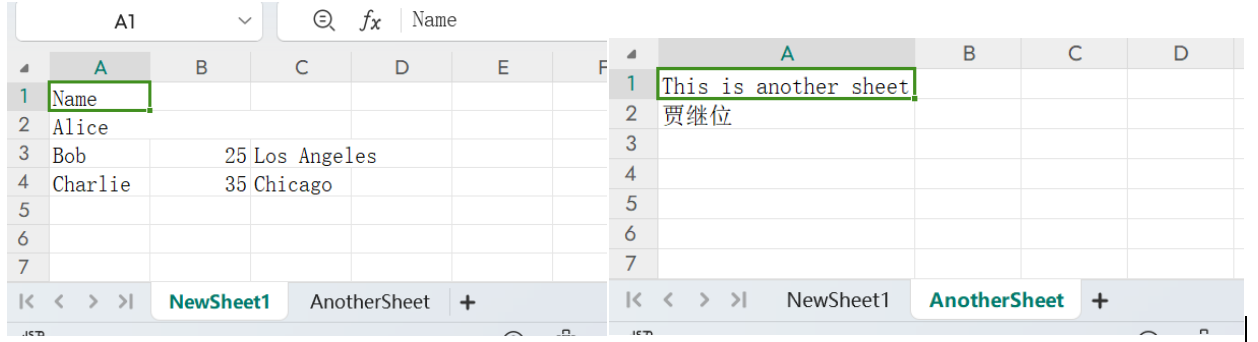
\includegraphics[width=0.8\textwidth]{part/自动化/办公自动化/pic/excel/openpyxl写入、合并演示.png}
        \caption{openpyxl写入、合并演示}
        \label{fig:openpyxl写入、合并演示}
\end{figure}


\section{修改Excel文件单元格内容}
\label{subsec:openpyxl修改现有的Excel文件}
如果想修改已存在的工作簿，只需将创建工作簿的\codeinline{openpyxl.Workbook()}方法替换为\codeinline{openpyxl.load\_workbook()}方法即可。

\section{修改Excel文件样式}
\label{subsec:openpyxl修改Excel文件样式}
\codeinline{openpyxl}支持设置单元格的样式，例如字体、颜色、对齐方式等。

主要分为以下几个部分:
\begin{enumerate}[label=\arabic*)]
    \item Font: 字体样式
    \item PatternFill: 填充样式
    \item Border: 边框样式
    \item Alignment: 对齐样式
\end{enumerate}

\subsection{基本样式}
\label{subsubsec:openpyxl基本样式}
\begin{lstlisting}[style=demostyle,numbers=none]
# openpyxl 的函数
## Font() 创建字体样式
## PatternFill() 创建填充样式
## Border() 创建边框样式
## Side() 创建边框样式
## Alignment() 创建对齐样式
## NamedStyle() 创建命名样式
## Style() 创建样式
\end{lstlisting}

\begin{lstlisting}[style=pythonstyle,numbers=left]
from openpyxl import Workbook
from openpyxl.styles import Font, PatternFill, Border, Side, Alignment

# 1. 创建一个新的工作簿和工作表
workbook = Workbook()
sheet = workbook.active
sheet.title = "StyledSheet"

# 2. 定义字体样式
font = Font(name='Arial', size=14, bold=True, italic=False, color='FF0000')
# 其中颜色也可以这样写 color=colors.RED

# 3. 定义不同的PatternFill效果
fill_types = [
    'solid', 'lightVertical', 'lightGray', 'gray0625', 'darkGray', 'gray125',
    'lightDown', 'lightHorizontal', 'darkDown', 'lightUp', 'lightTrellis', 'darkGrid',
    'darkTrellis', 'lightGrid', 'darkVertical', 'darkHorizontal', 'mediumGray', 'darkUp'
]

# 4. 定义边框样式和不同颜色
border_colors = ['FF0000', '00FF00', '0000FF', 'FFFF00', 'FF00FF', '00FFFF']
border_styles = [Border(
    left=Side(style='thin', color=color),
    right=Side(style='thin', color=color),
    top=Side(style='thin', color=color),
    bottom=Side(style='thin', color=color)
) for color in border_colors]

# 5. 定义对齐样式
alignment = Alignment(horizontal='center', vertical='center')

# 6. 将不同的PatternFill效果应用到不同单元格
for i, fill_type in enumerate(fill_types):
    print(f"Applying {fill_type} fill")
    fill = PatternFill(fill_type=fill_type, start_color='FFFF00', end_color='FFFF00')
    cell = sheet.cell(row=i + 1, column=1, value=f"{fill_type} fill")
    cell.font = font
    cell.fill = fill
    cell.border = border_styles[i % len(border_styles)]
    cell.alignment = alignment

# 7.设置行高和列宽
sheet.row_dimensions[1].height = 30 # 设置第一行的行高为30
sheet.column_dimensions['A'].width = 20 # 设置第一列的列宽为20

# 8. 保存工作簿    
workbook.save('styled_workbook_complete.xlsx')
print("Workbook saved as styled_workbook_complete.xlsx")
\end{lstlisting}

\begin{figure}[htpb]
        \centering
        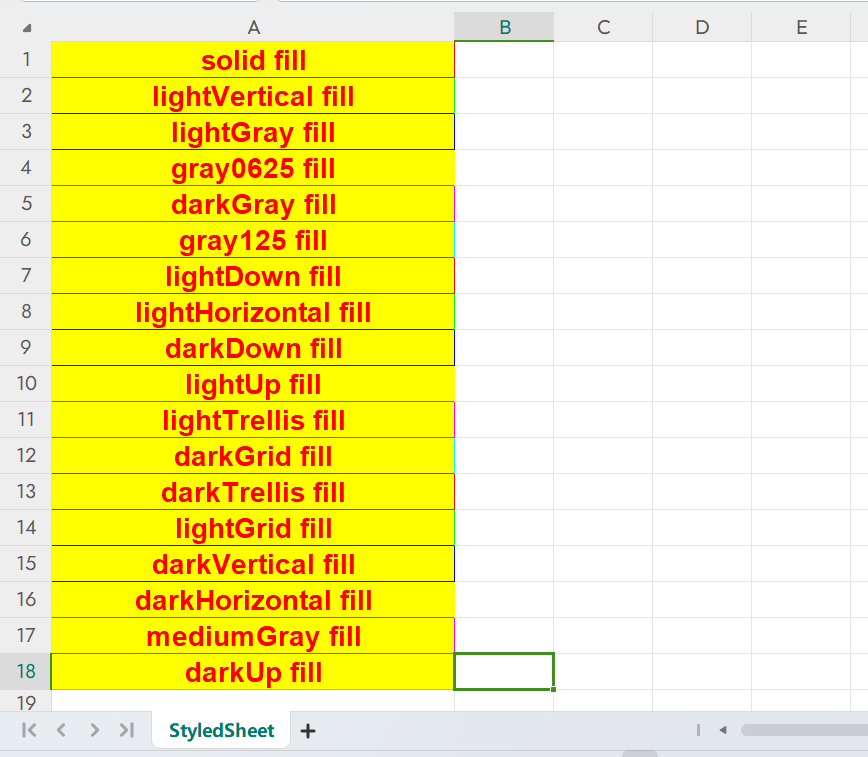
\includegraphics[width=0.8\textwidth]{part/自动化/办公自动化/pic/excel/openpyxl修改样式效果.png}
        \caption{openpyxl修改样式效果}
        \label{fig:openpyxl修改样式效果}
\end{figure}

\subsection{自定义样式}
\label{subsubsec:openpyxl自定义样式}
\begin{lstlisting}[style=pythonstyle,numbers=none]
from openpyxl import Workbook
from openpyxl.styles import Font, PatternFill, Border, Side, Alignment, NamedStyle

# 1. 创建一个新的工作簿和工作表
workbook = Workbook()
sheet = workbook.active
sheet.title = "StyledSheet"

# 2. 创建字体样式
font = Font(name='Arial', size=14, bold=True, italic=False, color='FF0000')

# 3. 创建填充样式
fill = PatternFill(fill_type='solid', start_color='FFFF00', end_color='FFFF00')

# 4. 创建边框样式
side = Side(style='thin', color='000000')
border = Border(left=side, right=side, top=side, bottom=side)

# 5. 创建对齐样式
alignment = Alignment(horizontal='center', vertical='center')

# 6. 将这些样式应用到特定单元格
cell = sheet.cell(row=1, column=1, value="Styled Text")
cell.font = font
cell.fill = fill
cell.border = border
cell.alignment = alignment

# 7. 创建命名样式
named_style = NamedStyle(name="highlight")
named_style.font = Font(name='Arial', size=12, bold=True, color='FFFFFF')
named_style.fill = PatternFill(fill_type='solid', start_color='FF5733')
named_style.border = Border(left=Side(style='thin', color='FF5733'),
                            right=Side(style='thin', color='FF5733'),
                            top=Side(style='thin', color='FF5733'),
                            bottom=Side(style='thin', color='FF5733'))
named_style.alignment = Alignment(horizontal='center', vertical='center')

# 注册命名样式
workbook.add_named_style(named_style)

# 应用命名样式到特定单元格
cell2 = sheet.cell(row=2, column=1, value="Named Style")
cell2.style = named_style

# 8. 保存工作簿
workbook.save('styled_workbook_complete.xlsx')
print("Workbook saved as styled_workbook_complete.xlsx")
\end{lstlisting}

\begin{figure}[htpb]
        \centering
        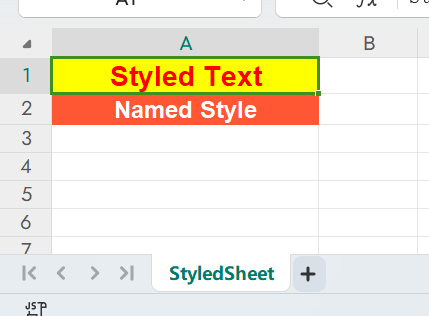
\includegraphics[width=0.8\textwidth]{part/自动化/办公自动化/pic/excel/openpyxl自定义样式效果.png}
        \caption{openpyxl自定义样式效果}
        \label{fig:openpyxl自定义样式效果}
\end{figure}

\section{操作大型Excel文件}
\label{subsec:openpyxl操作大型Excel文件}
当要处理大型工作簿时，直接将整个工作簿载人程序的操作是不合理的，数据量过大
会占用过多内存，从而影响程序本身的运行速度，导致程序出现“卡顿”、闪退等情况。

\codeinline{openpyxl}提供了一种更加高效的方式来处理大型工作簿，即使用\codeinline{read\_only}模式和\codeinline{write\_only}模式。

\begin{enumerate}[label=\arabic*)]
    \item 在\codeinline{read\_only}模式：

        openpyxl可以使用恒定的内存来处理无限的数据，其原理就是先处理一部分数据，处理完后，释放占用的内存，然后继续读入部分数据进行处理。这种方式可以快速读取大型工作簿中的数据。但需要注意，在该模式下，不允许对工作表进行写操作。

    \item 在\codeinline{write\_only}模式：

        openpyxl也是通过类似的原理将大量数据分批写入工作簿中的0
不同之处在于，该模式下不允许对工作表进行读操作。
\end{enumerate}

\subsection{read\_only模式}
\label{subsubsec:openpyxlread_only模式}
使用openpyxl的read only模式非常简单，只需在使用load\_workbook方法时将read only参数设置为True即可

\begin{lstlisting}[style=pythonstyle,numbers=left]
from openpyxl import load_workbook

# 在read_only模式下载入大型工作簿
wb = load_workbook('excel/large_workbook.xlsx', read_only=True)
# 选择 big_sheet1 工作表
sheet = workbook['big_sheet1']

for row in wb.iter_rows:  # 逐行读取数据
    for cell in row:      # 逐列读取数据
        print(cell.value)
\end{lstlisting}

\subsection{write\_only模式}
\label{subsubsec:openpyxlwrite_only模式}
使用openpyxl的write only模式也非常简单，只需在使用load\_workbook方法时将write only参数设置为True即可

\begin{lstlisting}[style=pythonstyle,numbers=left]
from openpyxl import Workbook
from openpyxl.cell import WriteOnlyCell
from openpyxl.comments import Comment
from openpyxl.styles import Font

# write_only 设置为 True
wb = Workbook(write_only=True)

# write_only模式下不会包含任何工作表，需要使用create_sheet方法自行仓U建
ws = wb.create_sheet()

# write_on1y模式下，单元格想要具有样式，就只能使用WriteOnlyCell创建单元格
cell = WriteOnlyCell (ws, 状态写入的内容')

# 为单元格设置字体样式
cell. font = Font (name='微软雅黑', size=36)

# 插入Excel批注
cell. comment = Comment (text='这是一个批注'，author='贾继伟')

# write_on1y模式下只能使用append方法添力口数据
## 在write_only模式下，不可在任意位置使用cell 或 iter_rows方法，
## 在添加数据时只能使用append方法
ws.append([cell, 2.333, None])

# 保存
wb save('write_only.xlsx')
\end{lstlisting}
\chapter{[必须安装Excel] xlwings库}

\section{简介}
使用xlwings\textcolor{red}{\textbf{必须}}安装Excel软件，xlwings是一个用于在Excel中调用Python的库，

\subsection{xlwings的数据结构}
\begin{figure}[htpb]
    \centering
    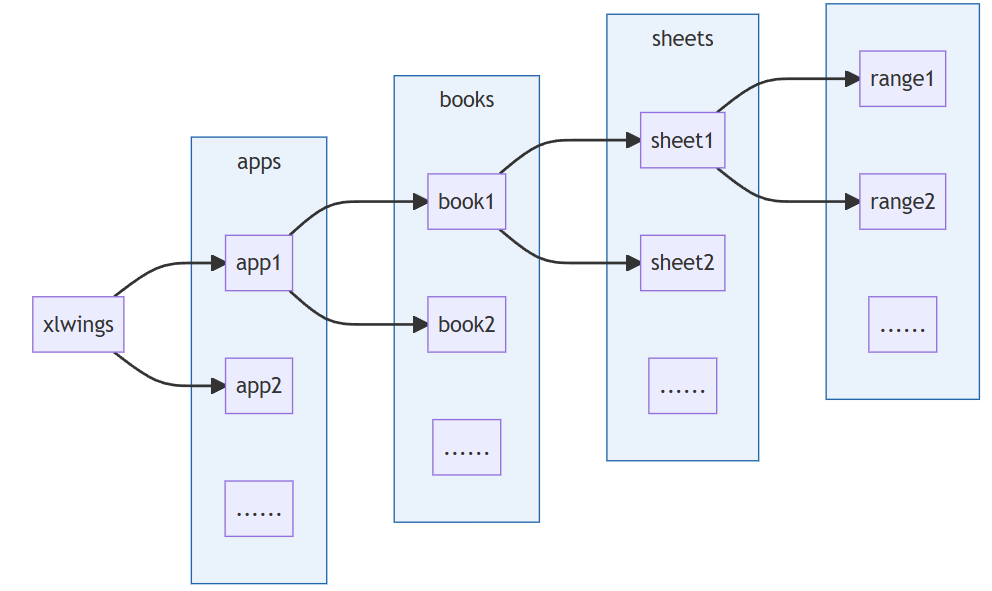
\includegraphics[width=0.6\textwidth]{part/自动化/办公自动化/pic/excel/xlwings/xlwings的数据结构.png}
    \caption{xlwings的数据结构}
    \label{fig:xlwings的数据结构}
\end{figure}
如图\ref{fig:xlwings的数据结构}所示，xlwings的数据结构主要有以下几个部分：
\begin{enumerate}[label=\arabic*)]
    \item App：单个Excel程序
    APP可以是一个Excel的实例，在此实例下创建工作薄，要创建工作簿，就必须先创建App实例。

    APP也可以是Excel程序集合,
    使用xlwings可以创建一个或者多个App,多个App之间是相互独立的,每个App对应一个PID值，PID值是数字编号，可以用来识别不同的App
    
    \item Book：单个工作簿

    \item Sheet：工作表

    \item Range: 单元格范围

\end{enumerate}


\section{安装}
\begin{lstlisting}[style=demostyle,numbers=none]
# pip 安装
pip install xlwings

pip install xlwings -i https://pypi.tuna.tsinghua.edu.cn/simple
# conda 安装
conda install xlwings
\end{lstlisting}

\section{App应用程序}
也正是因为App的存在，所以\codeinline{xlwings}必须安装Excel软件，否则无法使用xlwings库。

\begin{lstlisting}[style=demostyle,numbers=none]
import xlwings as xw
## App打开Excel
## visible = True 显示Excel界面
## add_book = False 不添加新的工作簿
app = xw.App(visible = True, add_book = False) 
# app = xw.App(visible = False, add_book = False) 

app.quit() # 关闭Excel
\end{lstlisting}

虽然新版的xlwings,可以直接对Book进行操作，
但是功能很有限，所以还是建议使用App来操作Excel。

\section{Book工作簿(Excel文件)}
工作簿的含义是Excel文件，可以通过xlwings创建一个新的工作簿

\subsection{新建/保存关闭工作簿}
\begin{lstlisting}[style=demostyle,numbers=none]
import xlwings as xw

# 1.创建一个新的工作簿
app = xw.App(visible = True, add_book = False) 
## 1.2 创建一个新的工作簿
wb = app.books.add()

# 2.保存工作簿
wb.save('test.xlsx')
wb.close() # 关闭工作簿
app.quit() # 关闭Excel
\end{lstlisting}

\subsection{获取当前活动工作簿}
\begin{lstlisting}[style=demostyle,numbers=none]
import xlwings as xw

# 获取当前活动的工作簿
active_wb = xw.books.active
\end{lstlisting}


\begin{lstlisting}[style=pythonstyle,numbers=left]
import xlwings as xw

app = xw.App(visible=True, add_book=False)
for i in range(1, 21):
    # 新建工作簿
    workbook = app.books.add()

    # 保存为特定文件名
    file_path = f'c:\\Users\\bingx\\Documents\\Python\\分公司{i}.xlsx'
    workbook.save(file_path)


    # 输出保存的文件路径（或名称）
    # print(f"已保存: {file_path}")
    
    workbook = app.books.open(file_path)  # 重新打开
    print(f"当前工作簿: {workbook.name}")

    # 关闭工作簿
    workbook.close()

# 关闭 Excel 应用
app.quit()
\end{lstlisting}
\begin{lstlisting}[style=demostyle,numbers=none]
前工作簿: 分公司1.xlsx
当前工作簿: 分公司2.xlsx
当前工作簿: 分公司3.xlsx
当前工作簿: 分公司4.xlsx
当前工作簿: 分公司5.xlsx
当前工作簿: 分公司6.xlsx
当前工作簿: 分公司7.xlsx
当前工作簿: 分公司8.xlsx
当前工作簿: 分公司9.xlsx
当前工作簿: 分公司10.xlsx
当前工作簿: 分公司11.xlsx
当前工作簿: 分公司12.xlsx
当前工作簿: 分公司13.xlsx
当前工作簿: 分公司14.xlsx
当前工作簿: 分公司15.xlsx
当前工作簿: 分公司16.xlsx
当前工作簿: 分公司17.xlsx
当前工作簿: 分公司18.xlsx
当前工作簿: 分公司19.xlsx
当前工作簿: 分公司20.xlsx
\end{lstlisting}

\subsection{删除工作簿}
xlwings 本身不能直接删除文件，但你可以结合 Python 的 \codeinline{os} 模块实现：
\begin{lstlisting}[style=demostyle,numbers=none]
import os

# 删除文件
file_path = 'test.xlsx'
os.remove(file_path)
\end{lstlisting}


\section{Sheet工作表(sheet)}
\subsection{新建工作表(sheet)}
\begin{lstlisting}[style=demostyle,numbers=none]
import xlwings as xw

# 1.创建一个新的工作簿
app = xw.App(visible = True, add_book = False) 
wb = app.books.add()

# 2.新建一个工作表
## 2.1 根据索引新建工作表
worksheet = wb.sheets[0] # 获取第一个工作表
worksheet.name = '员工信息' # 设置工作表的名称
## 2.2 在开头插入新的工作表
worksheet = wb.sheets.add('产品统计表') # 添加一个新的工作表
# 2.3在指定位置插入新的工作表
worksheet = wb.sheets.add('产品销售表', after='员工信息') # 添加一个新的工作表

# 3.保存工作簿
wb.save('test.xlsx')
wb.close() # 关闭工作簿
app.quit() # 关闭Excel
\end{lstlisting}
\begin{figure}[htpb]
    \centering
    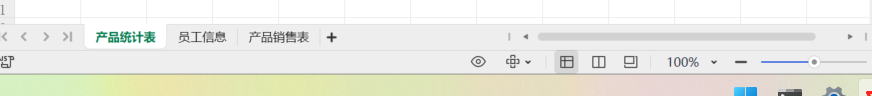
\includegraphics[width=0.4\textwidth]{part/自动化/办公自动化/pic/excel/xlwings/新建工作表演示.png}
    \caption{新建工作表演示}
    \label{fig:新建工作表演示}
\end{figure}

\subsubsection{获取工作表(sheet)}
\begin{enumerate}[label=\arabic*)]
    \item 按索引：\codeinline{wb.sheets[索引值]}, \textcolor{YBXPurple}{索引值从0开始}
    \item 按名称：\codeinline{wb.sheets['工作表名']}
    \item 当前活动工作表：\codeinline{wb.sheets.active}
    \item 获取所有工作表：\codeinline{wb.sheets}（返回所有工作表的集合）
\end{enumerate}

\subsubsection{按索引/名称获取工作表}
\begin{lstlisting}[style=demostyle,numbers=none]
import xlwings as xw

# 打开工作簿
wb = xw.Book('example.xlsx')

# 1.获取第一个工作表（索引从 0 开始）
sheet = wb.sheets[0]
print(sheet.name)  # 打印工作表名称

# 2.获取名为 'Sheet1' 的工作表
sheet = wb.sheets['Sheet1']
print(sheet.name)

# 3.获取当前活动的工作表
active_sheet = wb.sheets.active
print(active_sheet.name)
\end{lstlisting}


\subsection{获取工作簿中所有工作表}
\begin{lstlisting}[style=demostyle,numbers=none]
import xlwings as xw
wb = xw.Book("xlsx路径")
sheets = wb.sheets
\end{lstlisting}

\begin{lstlisting}[style=pythonstyle,numbers=left]    
import xlwings as xw
# 
wb = xw.Book("openpyxl/吉林2024-2021招生录取2024.11.14日姚老师校对基础表.xlsx")

# 获取工作簿中的所有工作表
sheets = wb.sheets

# 打印所有工作表的名称
print("工作簿中的所有工作表:")
for sheet in sheets:
    print(sheet.name)

# 关闭工作簿
wb.close()
\end{lstlisting}
\begin{lstlisting}[style=demostyle,numbers=none]
工作簿中的所有工作表:
录取表
普通专科物理
普通专科历史
普通本科物理
普通本科历史
提前A物理
提前A历史
查找表
错误名称表
\end{lstlisting}
\begin{figure}[htpb]
    \centering
    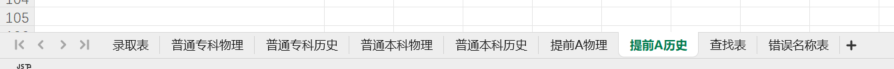
\includegraphics[width=0.6\textwidth]{part/自动化/办公自动化/pic/excel/xlwings/获取工作簿中所有工作表.png}
    \caption{获取工作簿中所有工作表}
    \label{fig:获取工作簿中所有工作表}
\end{figure}

\subsection{删除工作表(sheet)}
\begin{enumerate}[label=\arabic*)]
    \item 先获取工作表对象
    \item 然后调用 \codeinline{.delete()} 方法
\end{enumerate}

\begin{lstlisting}[style=demostyle,numbers=none]
# 删除指定工作表
sheet_to_delete = wb.sheets['Sheet1']
sheet_to_delete.delete()        
\end{lstlisting}

\subsection{重命名工作表}
\begin{enumerate}[label=\arabic*)]
    \item 先获取工作表对象
    \item 然后调用 \codeinline{.name} 属性
\end{enumerate}
\begin{lstlisting}[style=demostyle,numbers=none]
# 重命名工作表
sheet_to_rename = wb.sheets['Sheet1']
sheet_to_rename.name = '新名词'        
\end{lstlisting}

\section{Range区域/单元格}
具体对某个 Sheet 中行、列、单元格的操作，都是通过 \codeinline{sheet} 对象来实现的。
\subsection{获取单元格}
使用\codeinline{sheet.range}方法获取单元格，\codeinline{range}方法的参数可以是单元格的坐标，也可以是单元格的范围。
\begin{lstlisting}[style=demostyle,numbers=none]
# 获取单个单元格
cell = sheet.range('A1')

# 获取多个单元格
cells = sheet.range('A1:B3')
\end{lstlisting}

\begin{enumerate}[label=\arabic*)]
    \item 如果是单个单元格，返回的是 \codeinline{Range} 对象
    \item 如果多个单元格是一行/列，返回的是该行/列的 \codeinline{Range} 对象
    \item 如果多个单元格是一个矩形区域，返回的是该矩形区域的 \codeinline{Range} 对象，如图\ref{fig:xlwings_range获取某一区间}所示
\end{enumerate}

如果要获取单元格的值，可以使用 \codeinline{range.value} 属性：

\begin{figure}[htpb]
    \centering
    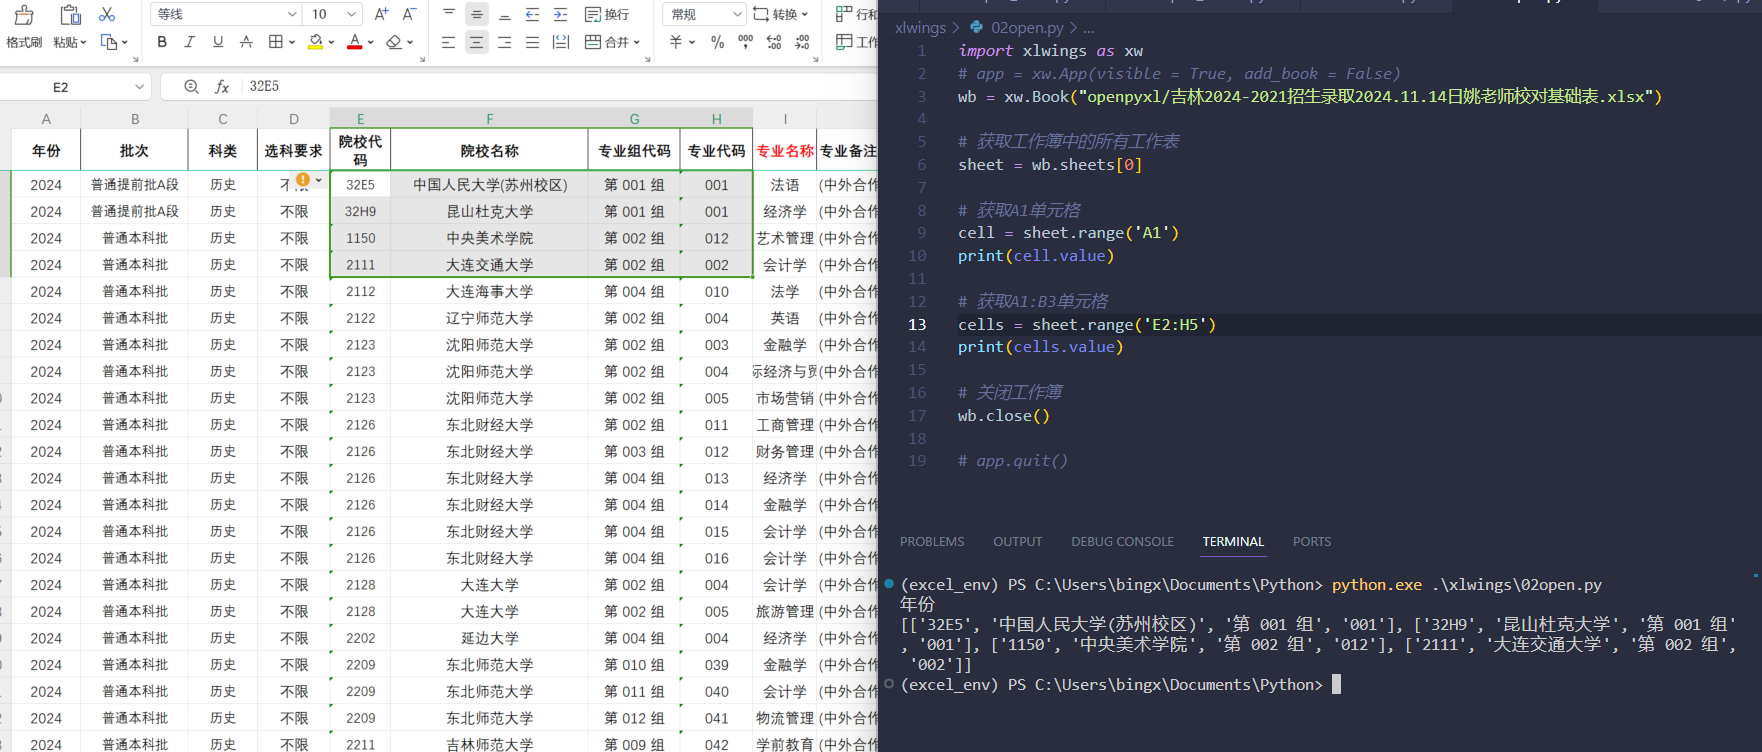
\includegraphics[width=0.6\textwidth]{part/自动化/办公自动化/pic/excel/xlwings/range获取某一区间.png}
    \caption{range获取某一区间}
    \label{fig:xlwings_range获取某一区间}
\end{figure}

\begin{lstlisting}[style=demostyle,numbers=none]
# 读取整行
row_values = sheet.range('1:1').value

# 读取整列
col_values = sheet.range('A:A').value
\end{lstlisting}

\subsection{清除单元格}
清除单元格的方法是 \codeinline{range.clear\_contents()},仅清除单元格内容（文字、数字、公式等）。
不改变工作表的结构（例如行列位置保持不变）。
\begin{lstlisting}[style=pythonstyle,numbers=left]   
import xlwings as xw

app = xw.App(visible=False, add_book=False)
wb = xw.Book("openpyxl/吉林2024-2021招生录取2024.11.14日姚老师校对基础表.xlsx")
sheet = wb.sheets[0]

# 清空A1:C3范围内的单元格
sheet.range('A1:C3').clear_contents()

wb.save("openpyxl/clear_contents.xlsx")
wb.close()
app.quit()
\end{lstlisting}

\begin{figure}[htpb]
    \centering
    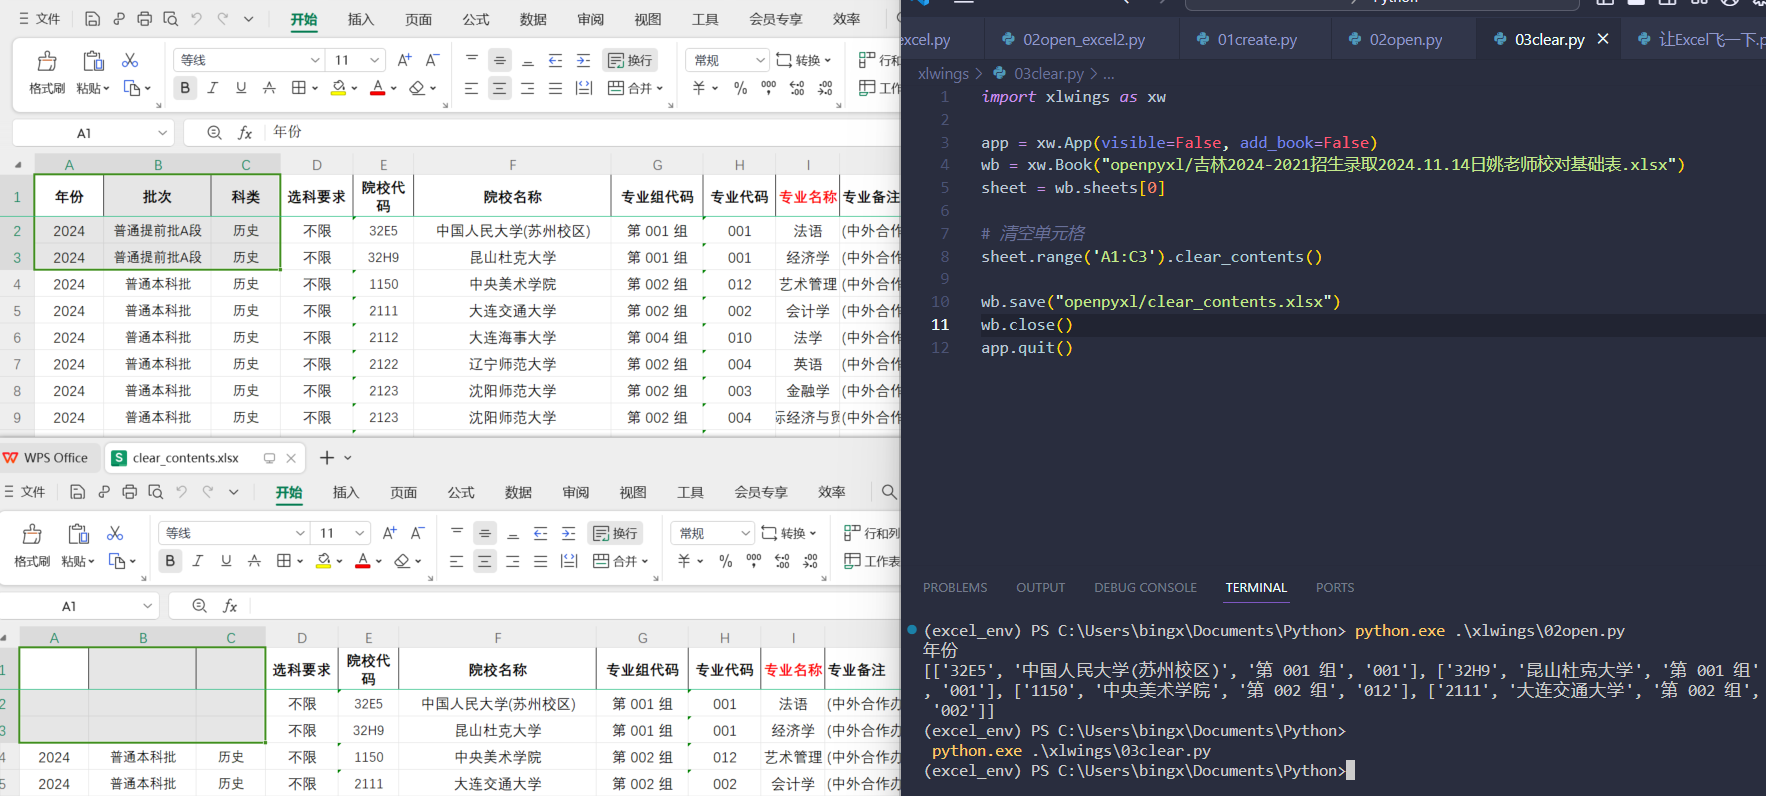
\includegraphics[width=0.6\textwidth]{part/自动化/办公自动化/pic/excel/xlwings/清空单元格演示.png}
    \caption{清空单元格演示}
    \label{fig:xlwings_清空单元格演示}
\end{figure}


\subsection{删除单元格}
删除单元格的方法是 \codeinline{range.delete(shift=None)},删除单元格后，影响到整个工作表的结构。
可选择向上或向左移动其余单元格。
\begin{enumerate}[label=\arabic*)]
    \item (\textcolor{red}{\textbf{不推荐}})\codeinline{shift=None}: 默认值，删除单元格后，不会移动其余单元格，
    但不一定有时候会移动其余单元格，不推荐使用

    \item \codeinline{shift='up'}: 删除单元格后，向上移动其余单元格
    \begin{figure}[htpb]
        \centering
        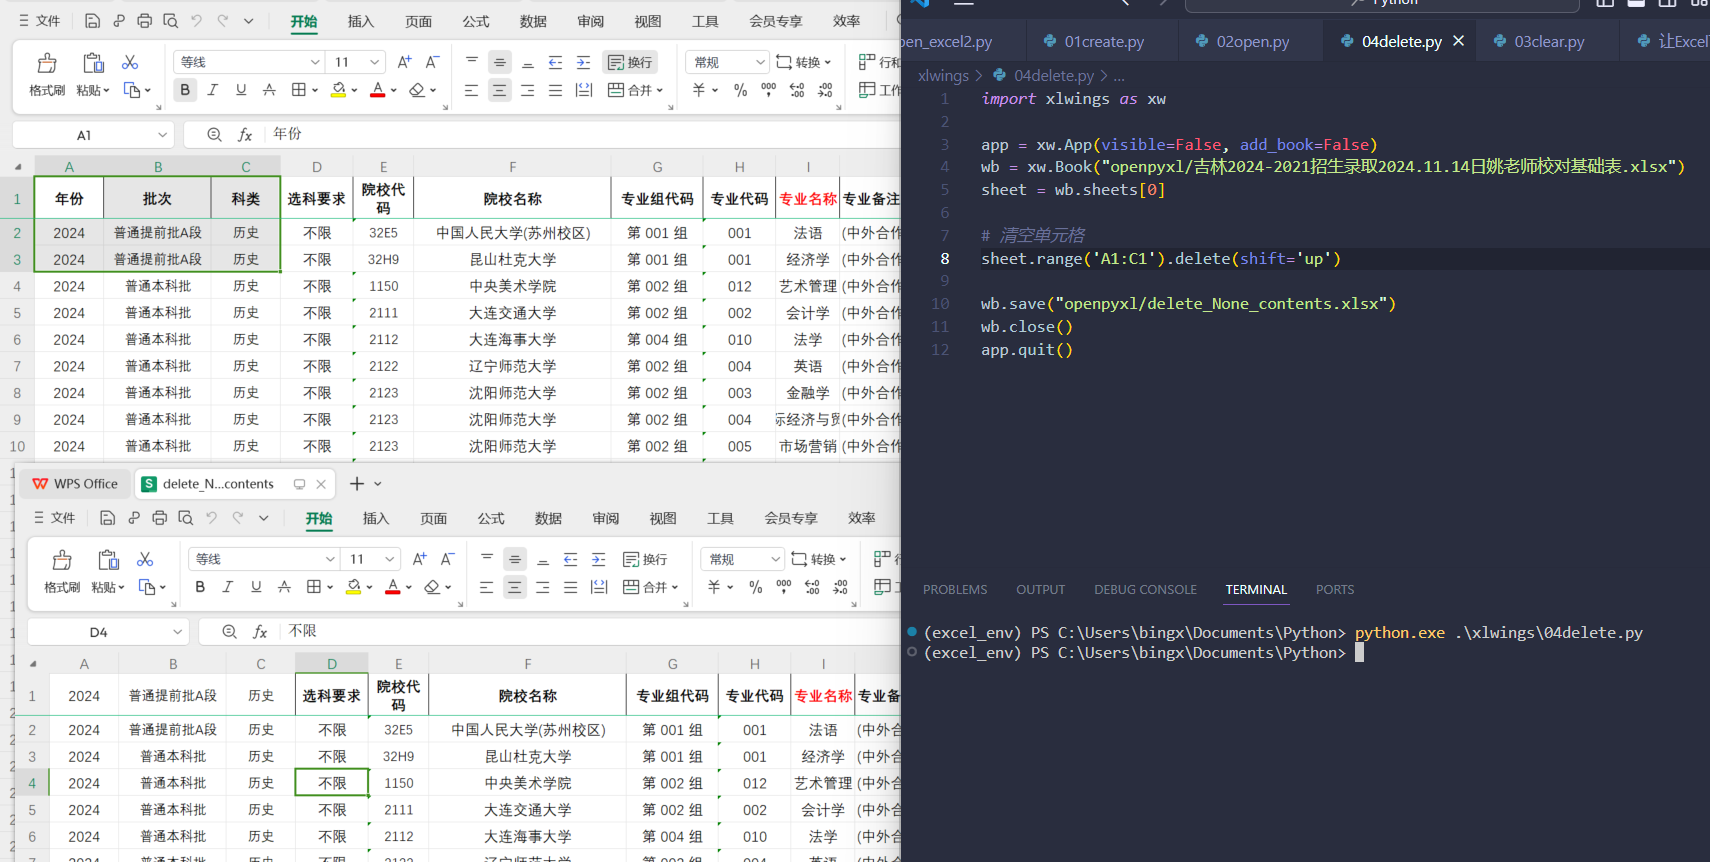
\includegraphics[width=0.6\textwidth]{part/自动化/办公自动化/pic/excel/xlwings/deleteshift=up效果.png}
        \caption{shift='up'效果}
        \label{fig:xlwings_deleteshift=up效果}
    \end{figure}
    
    \item \codeinline{shift='left'}: 删除单元格后，向左移动其余单元格
    \begin{figure}[htpb]
        \centering
        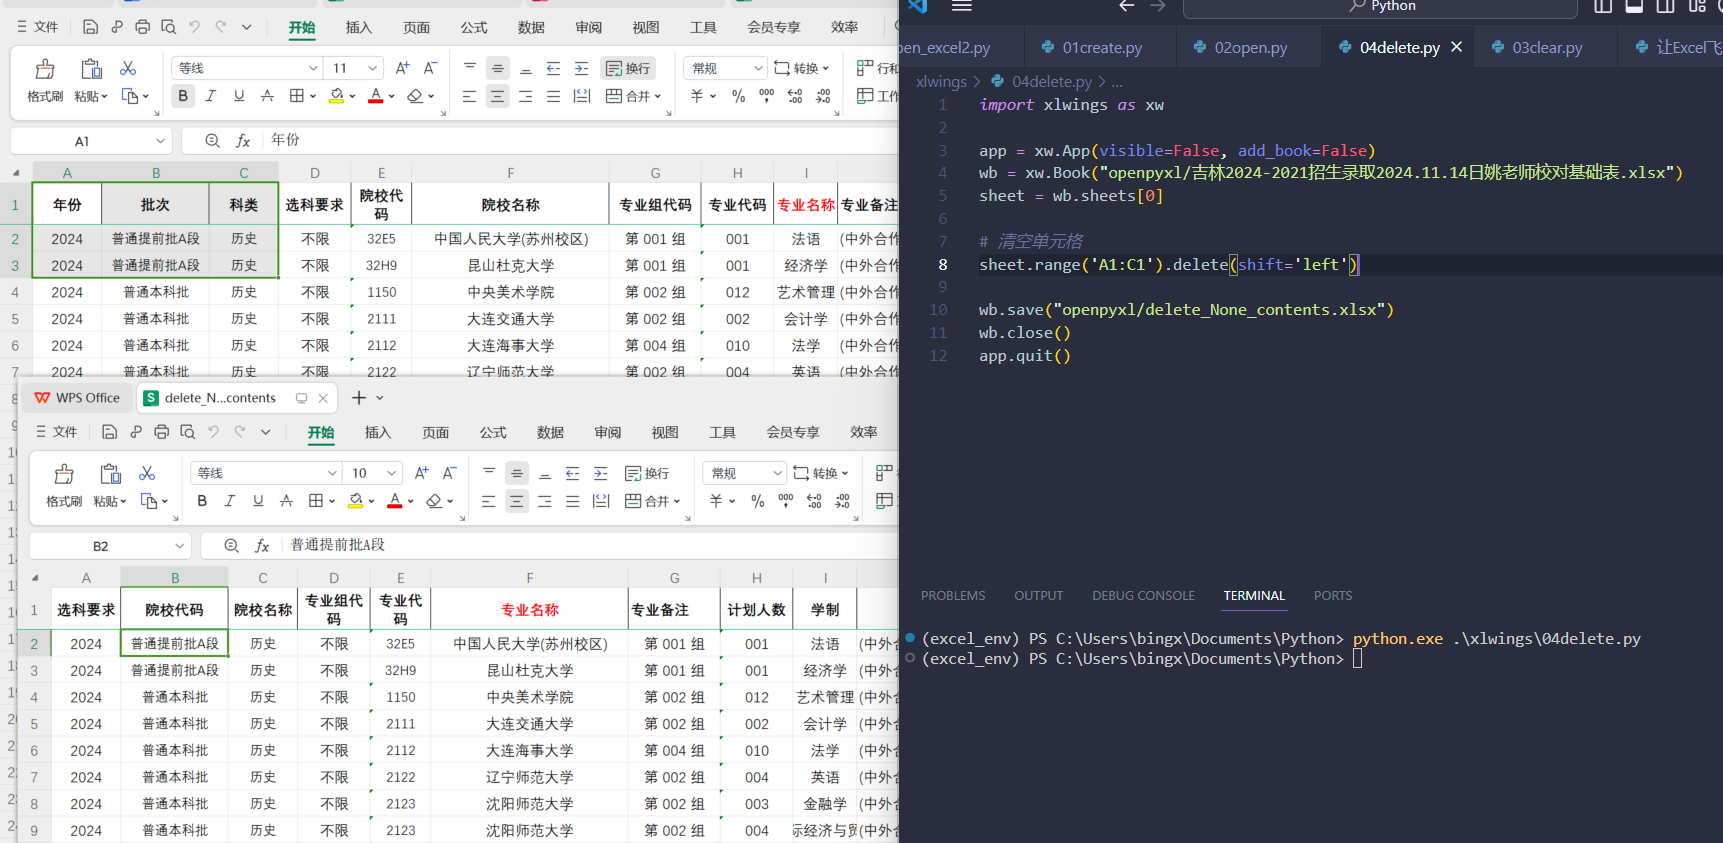
\includegraphics[width=0.6\textwidth]{part/自动化/办公自动化/pic/excel/xlwings/deleteshift=left效果.png}
        \caption{shift='left'效果}
        \label{fig:xlwings_deleteshift=left效果}
    \end{figure}
\end{enumerate}

\begin{lstlisting}[style=demostyle,numbers=none]
# 删除一行
sheet.range('1:1').delete()

# 删除一列
sheet.range('A:A').delete()
\end{lstlisting}


\subsection{插入单元格}
插入单元格的方法是 \codeinline{range.insert(shift=None)},插入单元格后，影响到整个工作表的结构。
可选择向下或向右移动其余单元格。
\begin{enumerate}[label=\arabic*)]
    \item (\textcolor{red}{\textbf{不推荐}})\codeinline{shift=None}: 默认值，插入单元格后，不会移动其余单元格，
    但不一定有时候会移动其余单元格，不推荐使用

    \item \codeinline{shift='down'}: 插入单元格后，向下移动其余单元格
    % \begin{figure}[htpb]
    %     \centering
    %     \includegraphics[width=0.6\textwidth]{part/自动化/办公自动化/pic/excel/xlwings/insertshift=down效果.png}
    %     \caption{shift='down'效果}
    %     \label{fig:xlwings_insertshift=down效果}
    % \end{figure}
    
    \item \codeinline{shift='right'}: 插入单元格后，向右移动其余单元格
    % \begin{figure}[htpb]
    %     \centering
    %     \includegraphics[width=0.6\textwidth]{part/自动化/办公自动化/pic/excel/xlwings/insertshift=right效果.png}
    %     \caption{shift='right'效果}
    %     \label{fig:xlwings_insertshift=right效果}
    % \end{figure}
\end{enumerate}

\begin{lstlisting}[style=demostyle,numbers=none]
# 插入一行
sheet.range('1:1').insert()

# 插入一列
sheet.range('A:A').insert()
\end{lstlisting}

\section{xlwings与panads的结合}
xlwings模块可以与pandas模块进行交互。

例如，用pandas模块创建数据表格，再用xlwings模块将表格写入工作簿，演示代码如下：
\begin{lstlisting}[style=demostyle,numbers=none]
import xlwings as xw
import pandas as pd
app = xw.App(visible=False)

# 创建一个新的工作簿
workbook = app.books.add()
worksheet = workbook.sheets.add('新工作表')

# 将DataFrame写入Excel
df = pd.DataFrame([[1, 2], [3, 4]], columns=['a', 'b'])
worksheet.range('B3').value = df # 在A1单元格写入DataFrame

# 保存工作簿
workbook.save(r'table.xlsx')
workbook.close()
app.quit()
\end{lstlisting}    
\begin{figure}[htpb]
    \centering
    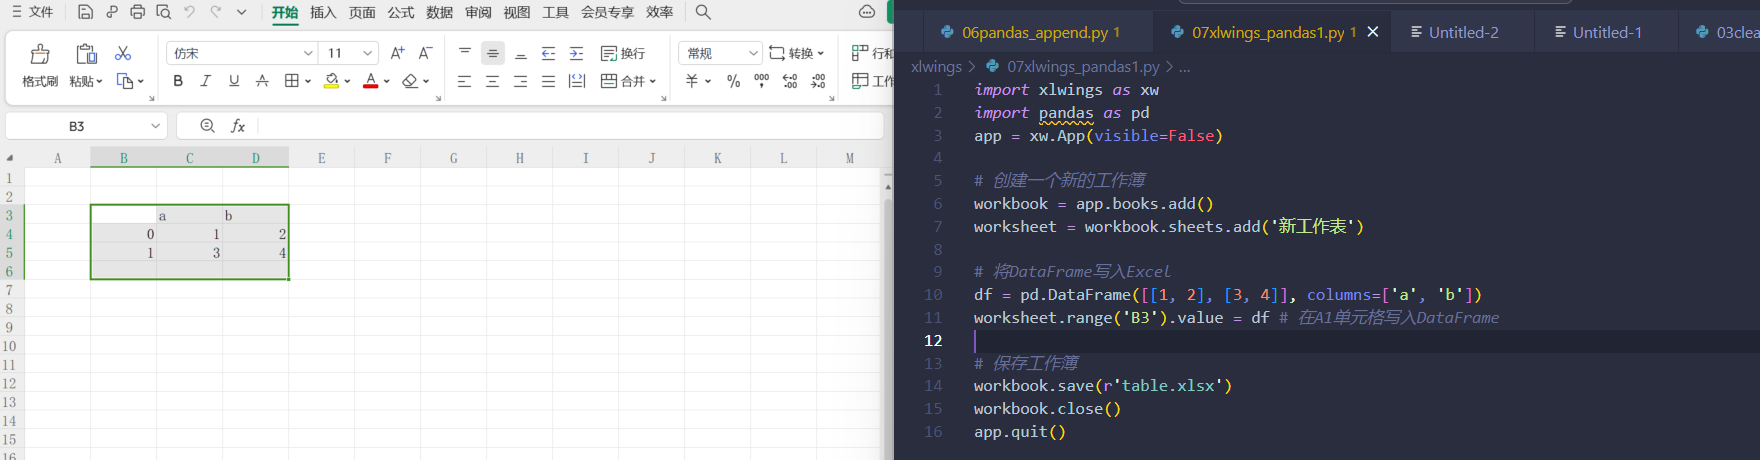
\includegraphics[width=0.6\textwidth]{part/自动化/办公自动化/pic/excel/xlwings/xlwings与pandas结合1.png}
    \caption{xlwings与pandas结合1}
    \label{fig:xlwings与pandas结合1}
\end{figure}
    



\chapter{word自动化}
\label{cha:word自动化}

\section{docx库}
\label{sec:docx库}
python-docx 是 Python 专门用来编辑 Word 文档的库，使用它的好处就是不必自己研究 docx 文件类型的底层实现细
节，你可以像操作.txt 文本一样直接打开、修改和保存关闭文件。可以说，python-docx
扩展库降低了用户使用 Python 的复杂度。

\subsection{安装}
\label{subsec:docx库安装}
\begin{lstlisting}[style=demostyle,numbers=none]
# pip 安装
pip install python-docx

# conda 安装
conda install python-docx
\end{lstlisting}

\subsection{创建Word文档}
\label{subsec:docx创建Word文档}
\begin{lstlisting}[style=pythonstyle,numbers=left]
import docx

doc = docx.Document() # Document对象表示整个文档
doc.add_heading('文章标题', 0) # 添加标题,0 表示标题的级别
doc.add_paragraph('Hello world!') # 添加段落
doc.add_heading('子标题', 1) # 添加标题,1 表示标题的级别
doc.add_paragraph('这是子标题段落') # 添加段落
doc.save('./word/docx创建文档.docx') # 保存文档
\end{lstlisting}




\chapter{web自动化}
\section{selenium介绍}
\href{https://www.selenium.dev/}{Selenium}是一个开源的测试工具，用于测试Web应用程序。
Selenium是一个用于测试Web应用程序的开源工具。它提供了一种简单的API，可以通过编程方式控制浏览器的行为，从而实现自动化测试。

\subsection{组成部分}
\begin{enumerate}[label=\arabic*)]
    \item Selenium WebDriver：这是 Selenium 的核心组件，用于直接与浏览器进行交互。WebDriver 提供了丰富的 API，允许开发者通过代码控制浏览器的行为，如打开网页、点击按钮、填写表单等。
    \item Selenium IDE：这是一个浏览器插件，主要用于录制和回放用户的操作。Selenium IDE 适合初学者快速创建简单的测试脚本，但它不支持复杂的逻辑和条件判断。
    \item Selenium Grid：这是一个用于并行执行测试的工具。通过 Selenium Grid，你可以在多个浏览器和操作系统上同时运行测试，从而加快测试速度并提高测试覆盖率。
\end{enumerate}

\subsection{Selenium WebDriver}
Selenium WebDriver 是 Selenium 的核心组件，它提供了与浏览器交互的 API，允许开发者通过编程语言控制浏览器并执行各种操作。

在 Selenium 4 中，引入了 \codeinline{Service} 对象来设置驱动程序路径，这种方式更加灵活，且符合 Selenium 4 的设计规范。

\section{selenium安装}
\begin{enumerate}[label=\arabic*)]
    \item pip安装selenium
\begin{lstlisting}[style=demostyle,numbers=none]
$> pip install selenium
$> pip show selenium
Name: selenium
Version: 4.38.0
Summary: Official Python bindings for Selenium WebDriver
Home-page: https://www.selenium.dev
Author:
Author-email:
License: Apache-2.0
Location: d:\application\miniconda\envs\pyauto\lib\site-packages
Requires: certifi, trio, trio-websocket, typing_extensions, urllib3, websocket-client
Required-by:
\end{lstlisting}

    \item 下载selenium驱动程序
 
    在selenium4.6以前的版本中，selenium需要下载对应的浏览器的驱动程序，才能进行自动化测试。
    \begin{table}
        \centering
        \begin{tabular}{|c|c|c|}
            \hline
            浏览器 & 驱动程序 & 下载地址 \\
            \hline
            Chrome & ChromeDriver & \href{https://sites.google.com/chromium.org/driver/}{点击下载} \\
            \hline
            Edge & EdgeDriver & \href{https://developer.microsoft.com/en-us/microsoft-edge/tools/webdriver/}{点击下载} \\
            \hline
            Firefox & GeckoDriver & \href{https://github.com/mozilla/geckodriver/releases}{点击下载} \\
            \hline
            Safari & SafariDriver & \href{https://webkit.org/blog/6900/webdriver-support-in-safari-10/}{点击下载} \\
            \hline
        \end{tabular}
    \end{table}
\end{enumerate}

\section{启动浏览器}
\begin{enumerate}[label=\arabic*)]
    \item selenium4.6以前的版本
\begin{lstlisting}[style=demostyle,numbers=none]
from selenium import webdriver

# 使用 Chrome 浏览器
driver = webdriver.Chrome(executable_path='/path/to/chromedriver')

# 或者使用 Firefox 浏览器
# driver = webdriver.Firefox(executable_path='/path/to/geckodriver')

# 或者使用 Edge 浏览器
# driver = webdriver.Edge(executable_path='/path/to/msedgedriver')
\end{lstlisting}

    \item selenium4.6及以后版本

    在 Selenium 4 中，不再直接在 webdriver.Chrome 中设置驱动程序路径，而是通过引入 Service 对象来设置。这样可以避免弃用警告，并确保驱动程序的正确加载。例如：
\begin{lstlisting}[style=demostyle,numbers=none]
from selenium import webdriver
driver = webdriver.Chrome() # 如果使用其他浏览器，如 Firefox，需要相应修改

# 访问网址
driver.get(f"https://www.baidu.com/")

# 保持浏览器不退出
s = input("输入回车退出")
\end{lstlisting}
\begin{figure}[htpb]
    \centering
    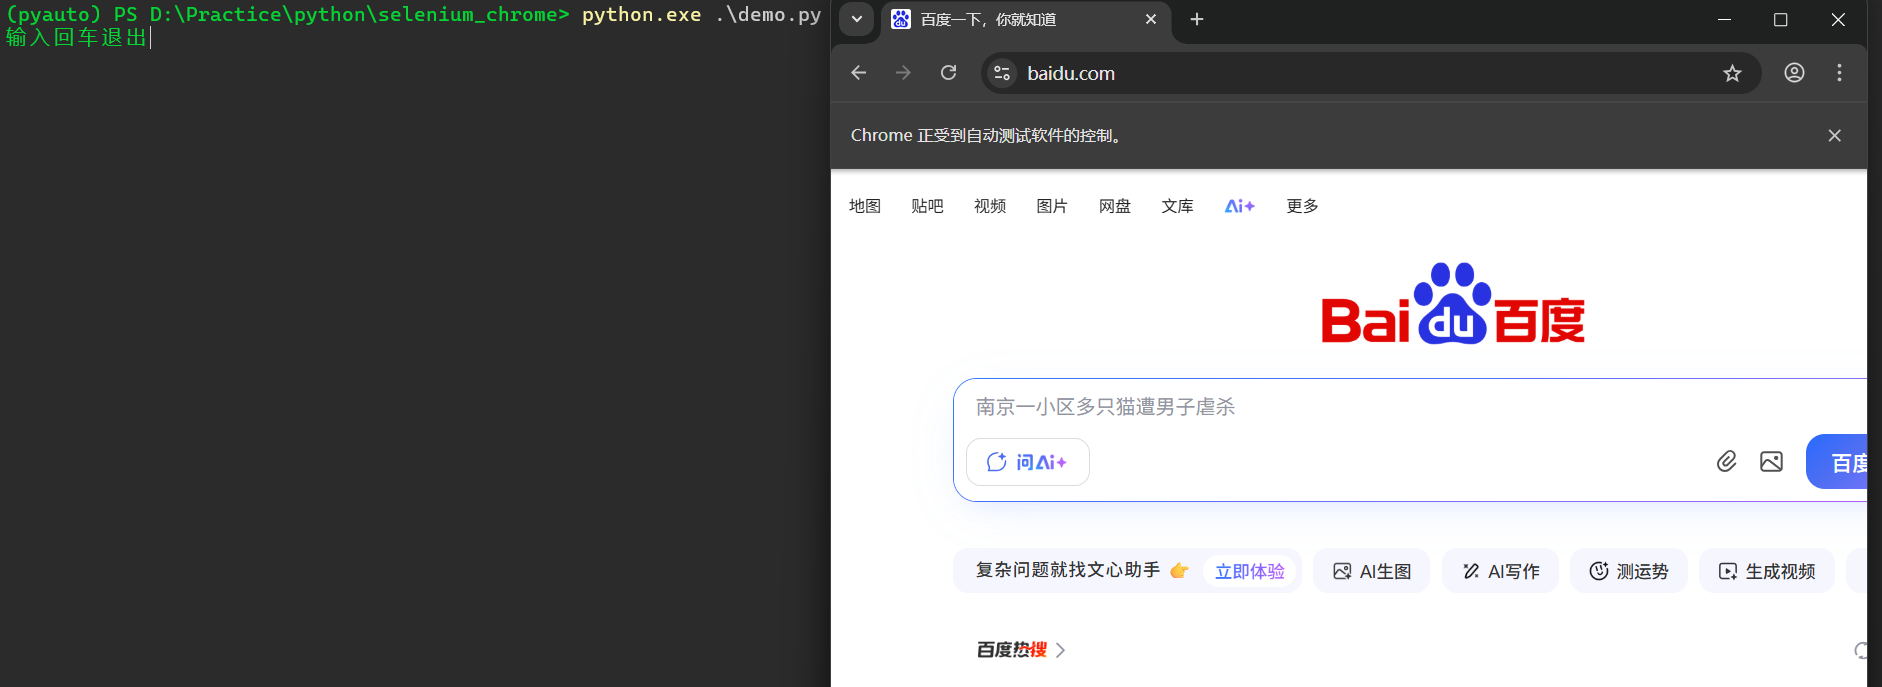
\includegraphics[width=0.6\textwidth]{part/自动化/网页自动化/pic/Selenium/概述/自动下载相应的驱动.png}
    \caption{Selenium4.0以后自动下载相应的驱动}
\end{figure}

\textcolor{red}{\textbf{当国内的网络环境，自动检测下载驱动需要不一样的网络环境，所以建议手动下载驱动，然后指定驱动路径。}}

\begin{lstlisting}[style=demostyle,numbers=none]
from selenium import webdriver
from selenium.webdriver.chrome.service import Service
# 在 Selenium 4 中，不再直接在 webdriver.Chrome 中设置驱动程序路径，而是通过引入 Service 对象来设置。
# 这样可以避免弃用警告，并确保驱动程序的正确加载。

service = Service("D:/Practice/python/selenium_chrome/chromedriver.exe") # ChromeDriver路径
browser = webdriver.Chrome(service=service)     # 创建浏览器对象

# 访问网址
browser.get(f"https://www.baidu.com/")  

# 定位元素

# 保持浏览器不退出
s = input("输入回车退出")
\end{lstlisting}
\begin{figure}[htpb]
    \centering
    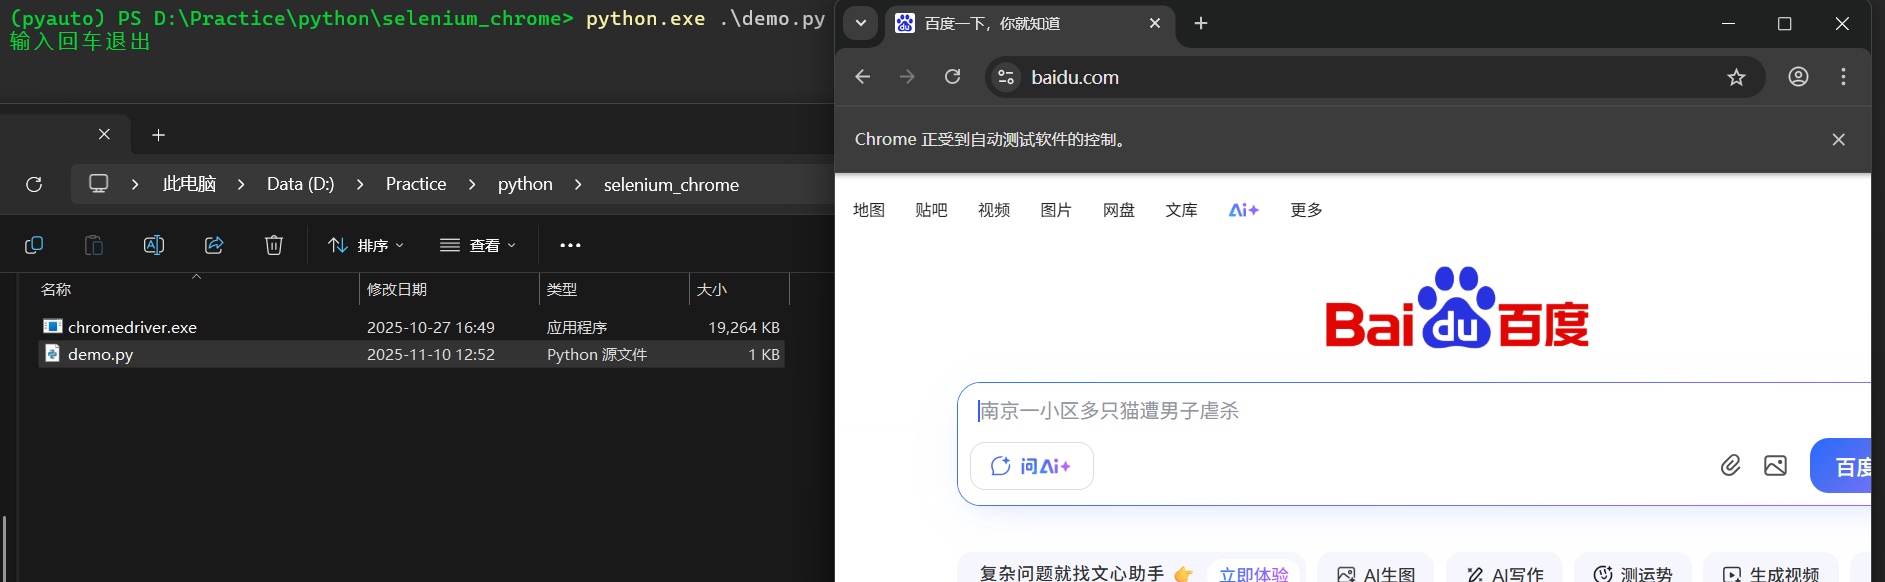
\includegraphics[width=0.6\textwidth]{part/自动化/网页自动化/pic/Selenium/概述/Selenium4指定驱动位置.png}
    \caption{Selenium4指定驱动位置}
\end{figure}
\end{enumerate}

\subsection{Selenium 操作流程}
\begin{lstlisting}[style=demostyle,numbers=none]
from selenium import webdriver
from selenium.webdriver.chrome.service import Service as ChromeService    

# 1.设置正确的驱动路径
service = ChromeService(executable_path="D:/Practice/python/selenium_chrome/chromedriver.exe")

# 2.[可选] 设置开机启动参数
options = webdriver.ChromeOptions() # 创建ChromeOptions对象
options.add_argument("--start-maximized") # 窗口最大化

# 3.创建浏览器对象
browser = webdriver.Chrome(service=service, options=options)

# 4.访问网址
browser.get(f"https://www.baidu.com/")

# 5.定位元素

# 6.操作元素

# 7.[可选] 保持浏览器不退出

# 7.[可选] 操作完成后关闭浏览器
browser.quit()
\end{lstlisting}



\input{part/自动化/通讯软件/邮件.tex}
\chapter{OCR识别}

\section{在线识别}

\section{离线识别}
\subsection{pytesseract}






% 书的索引
\cleardoublepage 
\phantomsection
\addcontentsline{toc}{chapter}{Index}
\RaggedRight
\thispagestyle{empty}
\printindex

\bibliographystyle{plain}
\bibliography{Ref}
\end{document} 



